\documentclass[12pt]{article}
\usepackage{frankstyle}

\begin{document}

\title{Using Invalid Instruments on Purpose: Focused Moment Selection and Averaging for GMM\footnote{I thank Aislinn Bohren, Gerda Claeskens, Bruce Hansen, Byunghoon Kang, Toru Kitagawa, Hannes Leeb, Serena Ng, Alexei Onatski, Hashem Pesaran, Benedikt P\"{o}tscher, Frank Schorfheide, Neil Shephard,  Richard J.\ Smith, Stephen Thiele, Melvyn Weeks, as well as seminar participants at Cambridge, the University of Vienna, Queen Mary, St Andrews, George Washington, UPenn, Columbia, Oxford, and the 2011 Econometric Society European Meetings for their many helpful comments and suggestions. I thank Kai Carstensen for providing data for my empirical example.}}

\author{Francis J.\ DiTraglia \\ University of Pennsylvania}

\date{\normalsize First Version: November 9, 2011 \\ This Version: \today}

\maketitle 
\begin{abstract}
	%!TEX root = main.tex
In finite samples, the use of a slightly endogenous but highly relevant instrument can reduce mean-squared error (MSE). Building on this observation, I propose a moment selection criterion for GMM in which moment conditions are chosen based on the MSE of their associated estimators rather than their validity: the focused moment selection criterion (FMSC). 
I then show how the framework used to derive the FMSC can address the problem of inference post-moment selection.
Treating post-selection estimators as a special case of moment-averaging, in which estimators based on different moment sets are given data-dependent weights, I propose  simulation-based procedures for inference that can be applied to a variety of formal and informal moment-selection and averaging procedures.
Both the FMSC and confidence interval procedures perform well in simulations.
I conclude with an empirical example examining the effect of instrument selection on the estimated relationship between malaria and income.

\end{abstract}

%Body of the paper
%!TEX root = main.tex
\section{Introduction}
In finite samples, the addition of an slightly endogenous but highly relevant instrument can yield a substantial improvement, reducing estimator variance by far more than bias is increased. 
Building on this observation, I propose a novel moment selection criterion for generalized method of moments (GMM) estimation: the focused moment selection criterion (FMSC). 
Rather than selecting only valid moment conditions, the FMSC chooses from a set of potentially mis-specified moment conditions to yield the minimum asymptotic mean squared error (AMSE) GMM estimator of a user-specified target parameter.
To ensure a meaningful bias-variance tradeoff in the limit, I employ a drifting asymptotic framework in which mis-specification, while present for any fixed sample size, vanishes asymptotically.
In the presence of such \emph{locally mis-specified} moment conditions, GMM remains consistent although, centered and rescaled, its limiting distribution displays an asymptotic bias. Adding an additional mis-specified moment condition introduces a further source of bias while reducing asymptotic variance. 
The idea behind the FMSC is to trade off these two effects in the limit as an approximation to finite sample behavior.\footnote{When finite-sample mean-squared error (MSE) is undefined or infinite, AMSE comparisons remain meaningful. In this case, one can view AMSE as the limit of a sequence of ``trimmed'' squared error loss functions, as in \cite{Hansen2013}. Trimmed MSE is always well-defined and the trimming fraction can be made asymptotically negligible.}
 
I consider a setting in which two blocks of moment conditions are available: one that is assumed correctly specified, and another that may not be.
This is intended to mimic the situation faced by an applied researcher who begins with a ``baseline'' set of maintained assumptions and must decide whether to impose any of a collection of stronger but also more controversial ``suspect'' assumptions.
To be credible, the baseline assumptions cannot be particularly strong.
As such, imposing one, or more, of the stronger suspect assumptions could yield more precise estimates, provided that the added assumption is at least \emph{nearly} correct.
When the (correctly specified) baseline moment conditions identify the model, the FMSC provides an asymptotically unbiased estimator of AMSE, allowing us to carry out risk-based selection over the suspect moment conditions.
When this is not the case, it remains possible to use the AMSE framework to carry out a sensitivity analysis. 

Continuing under the local mis-specification assumption, I show how the framework employed in the derivation of the FMSC can be used to address the important problem of inference post-moment selection.
I treat post-selection estimators as a special case of moment averaging: combining estimators based on different moment sets with data-dependent weights.
By deriving the limiting distribution of this class of estimators in general, I propose a simulation-based procedure for constructing valid confidence intervals. 
This technique can be applied to a variety of formal moment averaging and post-selection estimators, such as the FMSC, as well as pre-test estimators based on the $J$-- and Durbin-Hausman-Wu--statistic (DHW).

While the methods described here apply to general GMM models, subject to standard regularity conditions, I focus on two simple but empirically relevant examples: choosing between ordinary least squares (OLS) and two-stage least squares (TSLS) estimators, and selecting instruments in linear instrumental variables (IV) models. 
In the OLS versus TSLS example the FMSC takes a particularly intuitive and transparent form, providing a risk-based justification for the DHW test, and leading to a novel ``minimum-AMSE'' estimator that optimally combines the information contained in the OLS and TSLS estimators.
In simulation studies for both examples, the FMSC and confidence interval procedures perform well.
The cost, in terms of estimator risk, of using the FMSC rather than simply carrying out estimation under the baseline moment conditions is small; the gains, on the other hand, can be substantial.
I conclude with an empirical application from development economics, exploring the effect of instrument selection on the estimated relationship between malaria transmission and per capita income.

My approach to moment selection under mis-specification is inspired by the focused information criterion of \citet{ClaeskensHjort2003}, a model selection criterion for models estimated by maximum likelihood. 
Like them, I allow for mis-specification and study AMSE-based selection in a drifting asymptotic framework. 
In contradistinction, however, I consider moment rather than model selection, and general GMM rather than maximum likelihood estimators.
Although developed independently of the FIC, \cite{Schorfheide2005} uses a similar approach to select over forecasts constructed from mis-specified vector autoregression models.
Mine is by no means the first paper to consider GMM asymptotics under locally mis-specified moment conditions, an idea that dates at least as far back as \cite{Newey1985}.
The idea of using this framework for AMSE-based moment selection, however, is new to the literature. 

The FMSC differs substantially from existing criteria for moment selection under mis-specification whose primary aim is to consistently select all correctly specified moment conditions while eliminating all invalid ones.
This idea begins with \cite{Andrews1999}, who proposes a family of consistent moment selection criteria for GMM by adding an appropriate penalty term to the $J$-statistic. 
\cite{AndrewsLu} extend this work to allow simultaneous GMM moment and model selection, while \cite{HongPrestonShum} derive analogous results for generalized empirical likelihood.
More recently, \cite{Liao} proposes a shrinkage procedure for simultaneous GMM moment selection and estimation. 
Given a set of correctly specified moment conditions that identifies the model, this method consistently chooses all valid conditions from a second set of potentially mis-specified conditions.
In contrast to these proposals, which examine only the validity of the moment conditions under consideration, the FMSC balances validity against relevance to minimize AMSE.
Although \cite{HallPeixe2003} and \cite{ChengLiao} do consider relevance, their aim is to avoid including redundant moment conditions after consistently eliminating invalid ones.
In contrast to the FMSC, they do not allow for the intentional inclusion of a slightly invalid but highly relevant instrument to reduce AMSE. 
Some other papers that propose choosing, or combining, instruments to minimize MSE include \cite{DonaldNewey2001}, \cite{DonaldImbensNewey2009}, and \cite{KuersteinerOkui2010}.
Unlike the FMSC, however, these proposals consider the \emph{higher-order} bias that arises from including many valid instruments rather than the first-order bias that arises from the use of invalid instruments.

Another important difference between the FMSC and the other proposals from the literature is the ``F'' -- focus. 
Indeed, rather than a single moment selection criterion, the FMSC is really a method of constructing application-specific moment selection criteria.
Consider, for example, a simple dynamic panel model. If your target parameter is a long-run effect while mine is a contemporaneous effect, there is no reason to suppose \emph{a priori} that we should use the same moment conditions in estimation, even if we share the same model and dataset.
The FMSC explicitly takes this difference of research goals into account, unlike other moment selection criteria from the literature.

Like Akaike's Information Criterion (AIC), the FMSC is a conservative rather than consistent selection procedure.
As such, unlike the consistent moment selection criteria mdescribed above, it is random \emph{even in the limit}.
This may sound disconcerting.
Although consistency is a crucial minimal property in many settings, the situation is more complex for model and moment selection.
The problem is that consistent and conservative selection procedures have different strengths, but these strengths cannot be combined \cite{Yang2005}.
Which should be preferred depends on the application one has in mind.
If our goal is to evaulate the validity of an assumption from economic theory, consistent selection is the natural choice, as it will choose only correctly specified moment conditions with probability approaching one in the limit.
The motivation behind the FMSC, however, is to minimize estimator risk.
With this aim in mind, consistent selection criteria suffer from a serious defect: in general, unlike conservative criteria, they exhibit \emph{unbounded} minimax risk \cite{LeebPoetscher2008}.
Moreover, as discussed in more detail below, the asymptotics of consistent selection paint a seriously misleading picture of the effects of moment selection on inference.
For these reasons, the fact that the FMSC is conservative rather than consistent is a ``feature'' rather than a ``bug.''

Because it studies inference post-moment selection, this paper relates to a vast literature on ``pre-test'' and post-selection inference.
\citet{LeebPoetscher2005, LeebPoetscher2009} give a theoretical overview of the consequences of model selection for subsequent inference, while \cite{Demetrescu} illustrate them in a simulation study. 
There are several proposals to construct valid confidence intervals post-model selection, including \cite{Kabaila1998}, \cite{HjortClaeskens} and \cite{KabailaLeeb2006}. 
To my knowledge, however, this is the first paper to treat the problem in general for post-moment selection and moment average estimators in the presence of mis-specification.\footnote{Some related results appear in \cite{Berkowitz}, \cite{Guggenberger2010}, \cite{Guggenberger2012}, and \cite{GuggenbergerKumar}.}
While I developed the simulation-based, two-stage confidence interval procedure described below by analogy to \cite{ClaeskensHjortbook}, \cite{Leeb} kindly pointed out that similar constructions have appear in \cite{Loh1985}, \cite{Berger1994}, and \cite{Silvapulle1996}. More recently, \cite{McCloskey} takes a similar approach to study a class of non-standard testing problems.

The idea of treating post-moment selection estimators as a special case example of moment averaging, is adapted from the frequentist model average estimators of \cite{HjortClaeskens}.
Two other papers that consider weighting estimators based on different moment conditions are \cite{Xiao} and \cite{ChenChavezLinton}.
Whereas these papers combine estimators based on valid moment conditions to achieve a minimum variance estimator, however, I combine estimators based on potentially invalid conditions to minimize AMSE. 
A similar idea underlies the combined moments (CM) estimator of \cite{Judge2007}, who emphasize that incorporating the information from an incorrect specification could lead to favorable bias-variance tradeoff. 
Their proposal uses a Cressie-Read divergence measure to combine the information from competing moment specifications, for example OLS versus TSLS, yielding a data-driven compromise estimator. Unlike the FMSC, however, the CM estimator is not targeted to a particular research goal and does not explicitly aim to minimize AMSE.

An important limitation of the results presented here is that they are based upon the assumption of strong identification and a fixed number of moment conditions.
I do not, for example, consider weak-- or many--instrument asymptotics.
Extending the idea behind the FMSC to a more general framework that allows for weak identification and a growing number of moment conditions is a challenging and important topic that I leave for future research.

The remainder of the paper is organized as follows.
Section \ref{sec:asymp} describes the local mis-specification framework, introduces the two running examples, OLS versus TSLS and choosing instruments, and gives the main limiting results used later in the paper. 
Section \ref{sec:FMSC} derives FMSC as an asymptotically unbiased estimator of AMSE, presents specialized results for the two running examples, and examines their performance in a Monte Carlo experiment. 
Section \ref{sec:avg} describes a simulation-based procedure to construct valid confidence intervals for moment average estimators and examines its performance in a Monte Carlo experiment. Section \ref{sec:application} presents the empirical application and Section \ref{sec:conclude} concludes.
Proofs and computational details appear in the Appendix.
%!TEX root = main.tex
\section{Assumptions and Asymptotic Framework}
\label{sec:asymp}

\subsection{Local Mis-Specification}
Let $f(\cdot,\cdot)$ be a $(p+q)$-vector of moment functions of a random vector $Z$ and an $r$-dimensional parameter vector $\theta$, partitioned according to $f(\cdot,\cdot) = \left(g(\cdot,\cdot)', h(\cdot,\cdot)'  \right)'$ where $g(\cdot,\cdot)$ and $h(\cdot,\cdot)$ are $p$- and $q$-vectors of moment functions. 
The moment condition associated with $g$ is assumed to be correct whereas that associated with $h$ is locally mis-specified.
More precisely, 
\begin{assump}[Local Mis-Specification]
\label{assump:drift}
Let $\{Z_{ni}\colon 1\leq i \leq n, n =1, 2, \hdots\}$ be an iid triangular array of random vectors defined on a probability space $(\Upsilon, \mathcal{F}, \mathbb{P})$ satisfying
	\begin{enumerate}[(a)]
		\item $E[g(Z_{ni},\theta_0)] = 0$,
		\item $E[h(Z_{ni},\theta_0)] = n^{-1/2}\tau$, where $\tau$ is an unknown constant vector, 
		\item $\{f(Z_{ni},\theta_0)\colon 1\leq i \leq n, n = 1, 2, \hdots\}$ is uniformly integrable, and
		\item $Z_{ni} \rightarrow_d Z_i$.
	\end{enumerate}
\end{assump}
For any fixed sample size $n$, the expectation of $h$ evaluated at the true parameter value $\theta_0$ depends on the unknown constant vector $\tau$. 
Unless all components of $\tau$ are zero, some of the moment conditions contained in $h$ are mis-specified. In the limit however, this mis-specification vanishes, as $\tau/\sqrt{n}$ converges to zero. 
Uniform integrability combined with weak convergence implies convergence of expectations, so that $E[g(Z_i, \theta_0)]=0$ and $E[h(Z_i, \theta_0)]=0$. Because the limiting random vectors $Z_i$ are identically distributed, I suppress the $i$ subscript and simply write $Z$ to denote their common marginal law, e.g.\ $E[h(Z,\theta_0)]=0$. 
It is important to note that local mis-specification is \emph{not} intended as a literal description of real-world datasets: it is merely a device that gives asymptotic bias-variance trade-off that mimics the finite-sample intuition.
Moreover, while I work with an iid triangular array for simplicity, the results presented here can be adapted to handle dependent random variables.

\subsection{Candidate GMM Estimators}
Define the sample analogue of the expectations in Assumption \ref{assump:drift} as follows:
$$f_n(\theta) = \frac{1}{n}\sum_{i=1}^n f(Z_{ni},\theta) = \left[\begin{array}{c} g_n(\theta)\\ h_n(\theta) \end{array} \right]=\left[\begin{array}{c}n^{-1}\sum_{i=1}^n g(Z_{ni},\theta) \\ n^{-1}\sum_{i=1}^n h(Z_{ni},\theta) \end{array}\right]$$
where $g_n$ is the sample analogue of the correctly specified moment conditions and $h_n$ is that of the (potentially) mis-specified moment conditions.
A candidate GMM estimator $\widehat{\theta}_S$ uses some subset $S$ of the moment conditions contained in $f$ in estimation. 
Let $|S|$ denote the number of moment conditions used and suppose that $|S|>r$ so the GMM estimator is unique.\footnote{Identifying $\tau$ requires futher assumptions, as discussed in Section \ref{sec:ident}.} 
Let $\Xi_S$ be the $|S| \times(p +q)$ \emph{moment selection matrix} corresponding to $S$. That is, $\Xi_S$ is a matrix of ones and zeros arranged such that $\Xi_S f_n(\theta)$ contains only the sample moment conditions used to estimate $\widehat{\theta}_S$. 
Thus, the GMM estimator of $\theta$ based on moment set $S$ is given by 
$$\widehat{\theta}_S = \underset{\theta \in \Theta}{\mbox{arg min}}\; \left[\Xi_S f_n(\theta)\right]' \widetilde{W}_S \; \left[ \Xi_S f_n(\theta)\right].$$
where $\widetilde{W}_S$ is an $|S|\times |S|$, positive definite weight matrix.
There are no restrictions placed on $S$ other than the requirement that $|S| >r$ so the GMM estimate is well-defined. 
In particular, $S$ may \emph{exclude} some or all of the valid moment conditions contained in $g$.
While this may seem strange, it accommodates a wider range of examples, including choosing between OLS and TSLS estimators.

To consider the limit distribution of $\widehat{\theta}_S$, we require some further notation. 
First define the derivative matrices
	$$G = E\left[\nabla_{\theta} \; g(Z,\theta_0)\right], \quad H = E\left[\nabla_{\theta} \; h(Z,\theta_0)\right], \quad F = (G', H')'$$
and let $\Omega = Var\left[ f(Z,\theta_0) \right]$ where $\Omega$ is partitioned into blocks $\Omega_{gg}$, $\Omega_{gh}$, $\Omega_{hg}$, and $\Omega_{hh}$ conformably with the partition of $f$ by $g$ and $h$. 
Notice that each of these expressions involves the \emph{limiting random variable} $Z$ rather than $Z_{ni}$, so that the corresponding expectations are taken with respect to a distribution for which all moment conditions are correctly specified. 
Finally, to avoid repeatedly writing out pre- and post-multiplication by $\Xi_S$, define $F_S = \Xi_S F$ and $\Omega_S = \Xi_S \Omega\Xi_S'$. 
The following high level assumptions are sufficient for the consistency and asymptotic normality of the candidate GMM estimator $\widehat{\theta}_S$. 
\begin{assump}[High Level Sufficient Conditions]
\label{assump:highlevel} 
\mbox{}
	\begin{enumerate}[(a)]
		\item $\theta_0$ lies in the interior of $\Theta$, a compact set
		\item $\widetilde{W}_S \rightarrow_{p} W_S$, a positive definite matrix
		\item $W_S \Xi_S E[f(Z,\theta)]=0$ if and only if $\theta = \theta_0$
		\item $E[f(Z,\theta)]$ is continuous on $\Theta$
		\item $\sup_{\theta \in \Theta}\| f_n(\theta)- E[f(Z,\theta)]\|\rightarrow_{p} 0$
		\item $f$ is Z-almost surely differentiable in an open neighborhood $\mathcal{B}$ of $\theta_0$
		\item $\sup_{\theta \in \Theta} \|\nabla_{\theta}f_n(\theta) - F(\theta)\|\rightarrow_{p} 0$
		\item $\sqrt{n}f_n(\theta_0) \rightarrow_d  M + \left[\begin{array}{c}0\\ \tau \end{array} \right]$ where $M \sim N_{p+q}\left(0, \Omega \right)$
		\item $F_S'W_SF_S$ is invertible
	\end{enumerate}
\end{assump}

Although Assumption \ref{assump:highlevel} closely approximates the standard regularity conditions for GMM estimation, establishing primitive conditions for Assumptions \ref{assump:highlevel} (d), (e), (g) and (h) is slightly more involved under local mis-specification. 
Low-level sufficient conditions for the two running examples considered in this paper appear in Appendix \ref{sec:sufficient_conditions}.
For more general results, see \cite{Andrews1988} Theorem 2 and \cite{Andrews1992} Theorem 4.  
Notice that identification, (c), and continuity, (d), are conditions on the distribution of $Z$, the marginal law to which each $Z_{ni}$ converges. 

\begin{thm}[Consistency]
\label{thm:consist}
Under Assumptions \ref{assump:drift} and \ref{assump:highlevel} (a)--(e), $\widehat{\theta}_S \rightarrow_{p} \theta_0$.
\end{thm}

\begin{thm}[Asymptotic Normality]
\label{thm:normality}
Under Assumptions \ref{assump:drift} and \ref{assump:highlevel}
$$\sqrt{n}(\widehat{\theta}_S - \theta_0 ) \rightarrow_d -K_S \Xi_S  \left(\left[\begin{array}
	{c} M_g \\ M_h
\end{array} \right]  + \left[\begin{array}
	{c} 0 \\ \tau
\end{array} \right]\right)$$
where $K_S  = [F_S'W_SF_S]^{-1} F_S'W_S$, $M = (M_g', M_h')'$, and $M \sim N(0,\Omega)$.
\end{thm}

As we see from Theorems \ref{thm:consist} and \ref{thm:normality}, \emph{any} candidate GMM estimator $\widehat{\theta}_S$ is consistent for $\theta_0$ under local mis-specification. 
Unless $S$ excludes \emph{all} of the moment conditions contained in $h$, however, $\widehat{\theta}_S$ inherits an asymptotic bias from the mis-specification parameter $\tau$. 
The local mis-specification framework is useful precisely because it results in a limit distribution for $\widehat{\theta}_S$ with both a bias \emph{and} a variance. 
This captures in asymptotic form the bias-variance tradeoff that we see in finite sample simulations.
In constrast, fixed mis-specification results in a degenerate bias-variance tradeoff in the limit: scaling up by $\sqrt{n}$ to yield an asymptotic variance causes the bias component to diverge.

\subsection{Identification}
\label{sec:ident}
Any form of moment selection requires an identifying assumption: we need to make clear which parameter value $\theta_0$ counts as the ``truth.''
One approach, following \cite{Andrews1999}, is to assume that there exists a unique, maximal set of correctly specified moment conditions that identifies $\theta_0$. 
In the notation of the present paper\footnote{Although \cite{Andrews1999}, \cite{AndrewsLu}, and \cite{HongPrestonShum} consider \emph{fixed} mis-specification, we can view this as a version of local mis-specification in which $\tau \rightarrow \infty$ sufficiently fast.} this is equivalent to the following:

\begin{assump}[\cite{Andrews1999} Identification Condition]
	\label{assump:Andrews}
There exists a subset $S_{max}$ of at least $r$ moment conditions satisfying:
	\begin{enumerate}[(a)]
	 	\item $\Xi_{S_{max}} E[f(Z_{ni},\theta_0)]= 0$
	 	\item For any $S' \neq S_{max}$ such that $\Xi_{S'} E[f(Z_{ni},\theta')]= 0$ for some $\theta' \in \Theta$, $|S_{max}| > |S'|$.
	 \end{enumerate}
\end{assump}

\cite{AndrewsLu} and \cite{HongPrestonShum} take the same basic approach to identification, with appropriate modifications to allow for simultaneous model and moment selection. 
An advantage of Assumption \ref{assump:Andrews} is that, under fixed mis-specification, it allows consistent selection of $S_{max}$ without any prior knowledge of \emph{which} moment conditions are correct. 
In the notation of the present paper this corresponds to having no moment conditions in the $g$ block. As \citet[p.\ 254]{Hallbook} points out, however, the second part of Assumption \ref{assump:Andrews} can fail even in very simple settings.
When it does fail, the selected GMM estimator may no longer be consistent for $\theta_0$. 
A different approach to identification is to assume that there is a minimal set of at least $r$ moment conditions \emph{known} to be correctly specified.
This is the approach I follow here, as do \cite{Liao} and \cite{ChengLiao}.\footnote{For a dicussion of why Assumption \ref{assump:Identification} is necessary and how to proceed when it fails, see Appendix \ref{sec:digress}.}

\begin{assump}[FMSC Identification Condition] 
\label{assump:Identification}
Let $\widehat{\theta}_v$ denote the GMM estimator based solely on the moment conditions contained in the $g$--block
$$\widehat{\theta}_v = \underset{\theta \in \Theta}{\mbox{arg min}}\; g_n(\theta)' \widetilde{W}_{v} \; g_n(\theta)$$
We call this the ``valid estimator'' and assume that it satisfies all the conditions of Assumption \ref{assump:highlevel}. Note that this implies $p\geq r$.
\end{assump}

Assumption \ref{assump:Identification} and Theorem \ref{thm:normality} immediately imply that the valid estimator shows no asymptotic bias. 
\begin{cor}[Limit Distribution of Valid Estimator]
	\label{cor:valid}
	Let $S_{v}$ include only the moment conditions contained in $g$. 
	Then, under Assumption \ref{assump:Identification} we have
		$$\sqrt{n}\left(\widehat{\theta}_v - \theta_0\right) \rightarrow_d -K_v M_g$$
	by applying Theorem \ref{thm:normality} to $S_{v}$, where $K_v = [G'W_vG]^{-1}G'W_v$ and $M_g \sim N(0,\Omega_{gg})$. 
\end{cor}

Both Assumptions \ref{assump:Andrews} and \ref{assump:Identification} are strong, and neither fully nests the other. 
In the context of the present paper, Assumption \ref{assump:Identification} is meant to represent a situation in which an applied research chooses between two groups of assumptions.
The $g$--block contains the ``baseline'' assumptions while the $h$--block contains a set of stronger, more controversial ``suspect'' assumptions.
The FMSC is designed for settings in which the $h$--block is expected to contain a substantial amount of information beyond that already contained in the $g$--block. 
The idea is that, if we knew the $h$--block was correctly specified, we would expect a large gain in efficiency by including it in estimation. 
This motivates the idea of trading off the variance reduction from including $h$ against the potential increase in bias.
If the $h$--block assumptions are \emph{nearly correct} we may want to use them in estimation.
Not all applications have the structure, but many do.
Below, I consider two simple but empirically relevant examples: choosing between OLS and TSLS estimators and choosing instrumental variables.

%!TEX root = main.tex
\subsection{Example: OLS versus TSLS}
\label{sec:OLSvsIVlowlevel}
The simplest interesting application of the FMSC is choosing between ordinary least squares (OLS) and two-stage least squares (TSLS) estimators of the effect $\beta$ of a single endogenous regressor $x$ on an outcome of interest $y$. 
To keep the presentation transparent, I work within an iid, homoskedastic setting. 
Neither of these restrictions, however, is necessary. 
Without loss of generality assume that there are no exogenous regressors, or equivalently that they have been ``projected out of the system'' so that the data generating process is given by
    \begin{eqnarray}
			y_{i} &=& \beta x_{i}  + \epsilon_{i}\\
	x_{i} &=& \mathbf{z}_{i}' \boldsymbol{\pi} + v_{i}
	\end{eqnarray}
where $\beta$ and $\boldsymbol{\pi}$ are unknown constants, $\mathbf{z}_i$ is a vector of exogenous and relevant instruments, $x_i$ is the endogenous regressor, $y_i$ is the outcome of interest, and $\epsilon_i, v_i$ are unobservable error terms. 
All random variables in this system are mean zero, or equivalently all constant terms have been projected out. 
Stacking observations in the usual way, let 
$\mathbf{z}' = (z_{1}, \hdots, z_{n})$, $Z' = (\mathbf{z}_{1}, \hdots, \mathbf{z}_{n})$, $\mathbf{x}' = (x_{1}, \hdots, x_{n})$ and so on. The two estimators under consideration are $\widehat{\beta}_{OLS}$ and $\widetilde{\beta}_{TSLS}$, given by
  \begin{eqnarray} 
  \label{eq:OLS}
		\widehat{\beta}_{OLS} &=& \left(\mathbf{x}'\mathbf{x}\right)^{-1}\mathbf{x}'\mathbf{y}\\
	\label{eq:TSLS}
		\widetilde{\beta}_{TSLS} &=& \left(\mathbf{x}'P_Z\mathbf{x}\right)^{-1}\mathbf{x}'P_Z\mathbf{y}
	\end{eqnarray}
where $P_Z = Z(Z'Z)^{-1}Z'$. 
But why should we ever \emph{consider} using OLS if $x$ is endogenous and we have valid instruments at our disposal? 
The answer is simple: TSLS is a high variance estimator. 
Depending on the degree of endogeneity present in $x$ and the strength of the instruments, $\widehat{\beta}_{OLS}$ could easily have the lower mean-squared error of the two estimators.\footnote{Because the moments of the TSLS estimator only exist up to the order of overidentificiation \citep{Phillips1980} this statement should be understood to refer to ``trimmed'' mean-squared error when the number of instruments is two or fewer. See, e.g.\ \cite{Hansen2013}.} 
The appropriate version of the local mis-specification assumption for this example is as follows
  \begin{equation}
     E \left[\begin{array}{c} \mathbf{z}_{ni} \epsilon_{ni} \\ x_{ni} \epsilon_{ni} \end{array}\right] = \left[\begin{array}{c} \mathbf{0} \\ \tau/\sqrt{n} \end{array}\right]
  \end{equation}
where $\mathbf{0}$ is a vector of zeros, and $\tau$ is an unknown constant that encodes the endogeneity of $\tau$. 
In this setting, there is only a single moment condition in the $h$--block, namely $E[x_{ni}\epsilon_{ni}] = \tau/\sqrt{n}$. 
The question is not whether we should use this moment condition \emph{in addition} to the TSLS moment conditions written above it, but rather whether we should use it \emph{instead} of them.
The following simple low-level conditions are sufficient for the asymptotic normality of the OLS and TSLS estimators in this example.

\begin{assump}[OLS versus TSLS]
\label{assump:OLSvsIV}
	Let $\{(\mathbf{z}_{ni}, v_{ni}, \epsilon_{ni})\colon 1\leq i \leq n, n = 1, 2, \hdots\}$ be a triangular array of random variables such that
	\begin{enumerate}[(a)]
		\item $(\mathbf{z}_{ni}, v_{ni}, \epsilon_{ni}) \sim$ iid and mean zero within each row of the array (i.e.\ for fixed $n$)
		\item $E[\mathbf{z}_{ni} \epsilon_{ni}]=\mathbf{0}$, $E[\mathbf{z}_{ni} v_{ni}]=\mathbf{0}$, and $E[\epsilon_{ni}v_{ni}] = \tau/\sqrt{n}$ for all $n$
		\item $E[\left|\mathbf{z}_{ni}\right|^{4+\eta}] <C$, $E[\left|\epsilon_{ni}\right|^{4+\eta}] <C$, and $E[\left|v_{ni}\right|^{4+\eta}] <C$ for some $\eta >0$, $C <\infty$
		\item $E[\mathbf{z}_{ni} \mathbf{z}_{ni}'] \rightarrow Q>0$, $E[v_{ni}^2]\rightarrow \sigma_v^2 >0$, and $E[\epsilon_{ni}^2] \rightarrow \sigma_\epsilon^2 >0$ as $n\rightarrow \infty$
		\item As $n\rightarrow \infty$, $E[\epsilon_{ni}^2 \mathbf{z}_{ni} \mathbf{z}_{ni}']- E[\epsilon_{ni}^2]E[ \mathbf{z}_{ni} \mathbf{z}_{ni}'] \rightarrow 0$, $E[\epsilon_i^2 v_{ni} \mathbf{z}_{ni}'] - E[\epsilon_{ni}^2]E[v_{ni} \mathbf{z}_{ni}'] \rightarrow 0$, and $E[\epsilon_{ni}^2 v_{ni}^2] - E[\epsilon_{ni}^2]E[v_{ni}^2] \rightarrow 0$
		\item $x_{ni} = \mathbf{z}_{ni}'\boldsymbol{\pi} + v_i$ where $\boldsymbol{\pi} \neq \mathbf{0}$, and $y_{ni} = \beta x_{ni} + \epsilon_{ni}$
	\end{enumerate}
\end{assump}

Parts (a), (b) and (d) correspond to the local mis-specification assumption, part (c) is a set of moment restrictions, and (f) is simply the DGP.
Part (e) is the homoskedasticity assumption: an \emph{asymptotic} restriction on the joint distribution of $v_{ni}$, $\epsilon_{ni}$, and $\mathbf{z}_{ni}$. 
This condition holds automatically, given the other asssumptions, if $(\mathbf{z}_{ni}, v_{ni}, \epsilon_{ni})$ are jointly normal, as in our simulation experiment described below. 

\begin{thm}[OLS and TSLS Limit Distributions]
	\label{thm:OLSvsIV} Under Assumption \ref{assump:OLSvsIV},
	$$
\left[
\begin{array}{c}
  \sqrt{n}(\widehat{\beta}_{OLS} - \beta) \\
  \sqrt{n}(\widetilde{\beta}_{TSLS} - \beta)
\end{array}
\right] \overset{d}{\rightarrow}
N\left(
\left[
\begin{array}{c}
\tau/\sigma_x^2 \\ 
0
\end{array}
\right],\;
\sigma_\epsilon^2 \left[ \begin{array}{cc}
  1/\sigma_x^2 & 1/\sigma_x^2\\
  1/\sigma_x^2 & 1/\gamma^2 
  \end{array}\right]
  \right)
$$
where $\sigma_x^2 = \gamma^2 + \sigma_v^2$, $\gamma^2 = \boldsymbol{\pi}'Q \boldsymbol{\pi}$, and $Q$, $ \sigma_\epsilon^2$, and $\sigma_v^2$ are defined in Assumption \ref{assump:OLSvsIV}.
\end{thm}

We see from the preceding result that the variance of the OLS estimator is always strictly lower than that of the TSLS estimator since $\sigma^2_\epsilon/\sigma_x^2 = \sigma^2_\epsilon/(\gamma^2 + \sigma_v^2)$. 
Unless $\tau = 0$, however, OLS shows an asymptotic bias. 
In contrast, the TSLS estimator is asymptotically unbiased regardless of the value of $\tau$.  
%!TEX root = main.tex
\subsection{Example: Choosing Instrumental Variables}
\label{sec:chooseIVlowlevel}
The preceding example was quite specific, but in a sense it amounted to a problem of instrument selection: if $x$ is exogenous, it is clearly ``its own best instrument.'' 
Viewed from this perspective, the FMSC amounted to trading off endogeneity against instrument strength. I now consider instrument selection \emph{in general} for linear GMM estimators in an iid setting. 
Consider the following model:
\begin{eqnarray}
    y_i &=& \mathbf{x}_i' \beta +  \epsilon_i\\
    \mathbf{x}_i &=&  \Pi_1' \mathbf{z}_{i}^{(1)} + \Pi_2'\mathbf{z}_{i}^{(2)} + \mathbf{v}_i
\end{eqnarray}
where $y$ is an outcome of interest, $\mathbf{x}$ is an $r$-vector of regressors, some of which are endogenous, $\mathbf{z}^{(1)}$ is a $p$-vector of instruments known to be exogenous, and $\mathbf{z}^{(2)}$ is a $q$-vector  of \emph{potentially endogenous} instruments. 
The $r$-vector $\beta$, $p\times r$ matrix $\Pi_1$, and $q\times r$ matrix $\Pi_2$ contain unknown constants. Stacking observations in the usual way, let $\mathbf{y}' = (y_1, \hdots, y_n)$, $X' = (\mathbf{x}_1, \hdots, \mathbf{x}_n)$, $\boldsymbol{\epsilon} = (\epsilon_1, \hdots, \epsilon_n)$, 
$Z_1' = (\mathbf{z}_{1}^{(1)}, \hdots, \mathbf{z}_{n}^{(1)})$, $Z_2' = (\mathbf{z}_{1}^{(2)}, \hdots, \mathbf{z}_{n}^{(2)})$, and $V' = (\mathbf{v}_1, \hdots, \mathbf{v}_n)$ where $n$ is the sample size.
Using this notation, $\mathbf{y} = X\beta +\boldsymbol{\epsilon}$ and $X =  Z \Pi + V$, where $Z = (Z_1, Z_2)$ and $\Pi = (\Pi_1', \Pi_2')'$. 

The idea behind this setup is that the instruments contained in $Z_2$ are expected to be strong. 
If we were confident that they were exogenous, we would certainly use them in estimation. 
Yet the very fact that we expect them to be strongly correlated with $\mathbf{x}$ gives us reason to fear that the instruments contained in $Z_2$ may be endogenous. 
The exact opposite is true of $Z_1$. These are the instruments that we are prepared to assume are exogenous. 
But when is such an assumption plausible? Precisely when the instruments contained in $Z_1$ are \emph{not especially strong}. 
In this setting, the FMSC attempts to trade off a small increase in bias from using a \emph{slightly} endogenous instrument against a larger decrease in variance from increasing the overall strength of the instruments used in estimation.

To this end, consider a general linear GMM estimator of the form
$$\widehat{\beta}_S = (X'Z_S \widetilde{W}_S Z_S' X)^{-1}X'Z_S \widetilde{W}_S  Z_S' \mathbf{y}$$
where $S$ indexes the instruments used in estimation, $Z_S'  = \Xi_S Z'$ is the matrix containing only those instruments included in $S$, $|S|$ is the number of instruments used in estimation and $\widetilde{W}_S$ is an $|S|\times|S|$ positive semi-definite weighting matrix. In this example, the local mis-specification assumption is given by
\begin{equation}
  E\left[\begin{array}
    {c}
    \textbf{z}_{ni}^{(1)} (y_i - \textbf{x}_i\beta) \\
    \textbf{z}_{ni}^{(2)} (y_i - \textbf{x}_i \beta)
\end{array}\right] = \left[
  \begin{array}
    {c}
    \textbf{0} \\ \boldsymbol{\tau}/\sqrt{n}
  \end{array}
\right]
\end{equation}
where $\mathbf{0}$ is a $p$-vector of zeros, and $\boldsymbol{\tau}$ is a $q$-vector of unknown constants. 
The following low-level conditions are sufficient for the asymptotic normality of $\widehat{\beta}_S$.

\begin{assump}[Choosing IVs]
\label{assump:chooseIV} 
	Let $\{(\mathbf{z}_{ni}, \mathbf{v}_{ni}, \epsilon_{ni})\colon 1\leq i \leq n, n = 1, 2, \hdots\}$ be a triangular array of random variables with $\mathbf{z}_{ni} = (\mathbf{z}_{ni}^{(1)}$, $\mathbf{z}_{ni}^{(1)})$ such that
	\begin{enumerate}[(a)]
		\item $(\mathbf{z}_{ni}, \mathbf{v}_{ni}, \epsilon_{ni}) \sim$ iid within each row of the array (i.e.\ for fixed $n$)
		\item $E[\mathbf{v}_{ni}\mathbf{z}_{ni}']=\mathbf{0}$, $E[\mathbf{z}^{(1)}_{ni} \epsilon_{ni}]=\mathbf{0}$, and $E[\mathbf{z}^{(2)}_{ni} \epsilon_{ni}] = \boldsymbol{\tau}/\sqrt{n}$ for all $n$
		\item $E[\left|\mathbf{z}_{ni}\right|^{4+\eta}] <C$, $E[\left|\epsilon_{ni}\right|^{4+\eta}] <C$, and $E[\left|\mathbf{v}_{ni}\right|^{4+\eta}] <C$ for some $\eta >0$, $C <\infty$
		\item $E[\mathbf{z}_{ni} \mathbf{z}_{ni}'] \rightarrow Q>0$ and $E[\epsilon_{ni}^2 \mathbf{z}_{ni} \mathbf{z}_{ni}'] \rightarrow \Omega >0$ as $n\rightarrow \infty$
		\item $\mathbf{x}_{ni} =  \Pi_1' \mathbf{z}_{ni}^{(1)} + \Pi_2'\mathbf{z}_{ni}^{(2)} + \mathbf{v}_{ni}$ where $\Pi_1 \neq \mathbf{0}$, $\Pi_2 \neq \mathbf{0}$, and $y_i = \mathbf{x}_{ni}' \beta +  \epsilon_{ni}$
	\end{enumerate}
\end{assump}

The preceding conditions are similar to although more general than those contained in Assumption \ref{assump:OLSvsIV}. 
Although I no longer assume homoskedasticity, for simplicity I retain the assumption that the triangular array is iid in each row. 

\begin{thm}[Choosing IVs Limit Distribution]
\label{thm:chooseIV} Suppose that $\widetilde{W}_S \rightarrow_p W_S >0$. Then, under Assumption \ref{assump:chooseIV}
$$\sqrt{n}\left(\widehat{\beta}_S - \beta \right) \overset{d}{\rightarrow} -K_S \Xi_S \left(\left[\begin{array}
           {c} \mathbf{0} \\ \boldsymbol{\tau}
         \end{array}\right] + M \right)$$
where
         $$-K_S = \left(\Pi' Q_S W_S Q_S'\Pi\right)^{-1} \Pi'Q_SW_S$$
$M \sim N(\mathbf{0}, \Omega)$, $Q_S = Q \Xi_S'$, and $Q$ and $\Omega$ are defined in Assumption \ref{assump:chooseIV}.
\end{thm}
%!TEX root = main.tex
\section{The Focused Moment Selection Criterion}
\label{sec:FMSC}

\subsection{The General Case}
The FMSC chooses among the potentially invalid moment conditions contained in $h$ based on the estimator AMSE of a user-specified scalar target parameter.\footnote{Although I focus on the case of a scalar target parameter in the body of the paper, the same idea can be applied to a vector of target parameters. For details see Appendix \ref{append:mult}.}
Denote this target parameter by $\mu$, a real-valued, $Z$-almost continuous function of the parameter vector $\theta$ that is differentiable in a neighborhood of $\theta_0$. 
Further, define the GMM estimator of $\mu$ based on $\widehat{\theta}_S$ by $\widehat{\mu}_S = \mu(\widehat{\theta}_S)$ and the true value of $\mu$ by $\mu_0 = \mu(\theta_0)$. 
Applying the Delta Method to Theorem \ref{thm:normality} gives the AMSE of $\widehat{\mu}_S$.

\begin{cor}[AMSE of Target Parameter]
\label{cor:target}
Under the hypotheses of Theorem \ref{thm:normality}, 
$$\sqrt{n}\left(\widehat{\mu}_S - \mu_0\right)\rightarrow_d-\nabla_\theta\mu(\theta_0)'K_S \Xi_S \left(M +  \left[\begin{array}
	{c} 0 \\ \tau
\end{array} \right]\right)$$ 
where $M$ is defined in Theorem \ref{thm:normality}.
Hence,
	$$\mbox{AMSE}\left(\widehat{\mu}_S\right) = \nabla_\theta\mu(\theta_0)'K_S \Xi_S \left\{\left[\begin{array}{cc}0&0\\0&\tau\tau'\end{array}\right] + \Omega\right\}\Xi_S'K_S'\nabla_\theta\mu(\theta_0).$$
\end{cor}

For the valid estimator $\widehat{\theta}_v$ we have $K_v = \left[G'W_{v}G\right]^{-1}G' W_{v}$ and $\Xi_v =\left[\begin{array}{cc} \mathbf{I}_p& \mathbf{0}_{p\times q} \end{array} \right]$. 
Thus, the valid estimator $\widehat{\mu}_v$ of $\mu$ has zero asymptotic bias. 
In contrast, any candidate estimator $\widehat{\mu}_S$ that includes moment conditions from $h$ inherits an asymptotic bias from the corresponding elements of $\tau$, the extent and direction of which depends both on $K_S$ and $\nabla_\theta\mu(\theta_0)$. 
The setting considered here, however, is one in which using moment conditions from $h$ in estimation will reduce the asymptotic variance.
In the nested case, where moment conditions from $h$ are \emph{added} to those of $g$, this follows automatically.
The usual proof that adding moment conditions cannot increase asymptotic variance under efficient GMM \citep[see for example][ch.\ 6]{Hallbook} continues to hold under local mis-specification, because all moment conditions are correctly specified in the limit.
In non-nested examples, for example when $h$ contains OLS moment conditions and $g$ contains IV moment conditions, however, this result does not apply because one would use $h$ \emph{instead of} $g$.
In such examples, one must establish an analogous ordering of asymptotic variances by direct calculation, as I do below for the OLS versus IV example.

Using this framework for moment selection requires estimators of the unknown quantities: $\theta_0$, $K_S$, $\Omega$, and $\tau$. 
Under local mis-specification, the estimator of $\theta$ under \emph{any} moment set is consistent. 
A natural estimator is $\widehat{\theta}_v$, although there are other possibilities. 
Recall that $K_S = [F_S'W_SF_S]^{-1} F_S'W_S \Xi_S$.
Because it is simply the selection matrix defining moment set $S$, $\Xi_S$ is known.  
The remaining quantities $F_S$ and $W_S$ that make up $K_S$ are consistently estimated by their sample analogues under Assumption \ref{assump:highlevel}.
Similarly, consistent estimators of $\Omega$ are readily available under local mis-specification, although the precise form depends on the situation.\footnote{See Sections \ref{sec:OLSvsIVExample} and \ref{sec:chooseIVexample} for discussion of this point for the two running examples.}
The only remaining unknown is $\tau$. Local mis-specification is essential for making meaningful comparisons of AMSE because it prevents the bias term from dominating the comparison. 
Unfortunately, it also prevents consistent estimation of the asymptotic bias parameter.
Under Assumption \ref{assump:Identification}, however, it remains possible to construct an \emph{asymptotically unbiased} estimator $\widehat{\tau}$ of $\tau$ by substituting $\widehat{\theta}_v$, the estimator of $\theta_0$ that uses only correctly specified moment conditions, into $h_n$, the sample analogue of the potentially mis-specified moment conditions. 
In other words,  $\widehat{\tau} = \sqrt{n} h_n(\widehat{\theta}_v)$. 

\begin{thm}[Asymptotic Distribution of $\widehat{\tau}$] 
\label{thm:tau}
Let $\widehat{\tau} = \sqrt{n} h_n(\widehat{\theta}_v)$ where $\widehat{\theta}_v$ is the valid estimator, based only on the moment conditions contained in $g$. 
Then under Assumptions \ref{assump:drift}, \ref{assump:highlevel} and \ref{assump:Identification}
$$\widehat{\tau} \rightarrow_d \Psi\left( M + \left[\begin{array}
	{c} 0 \\ \tau
\end{array} \right]\right), \quad \Psi = \left[\begin{array}{cc} -HK_v & \mathbf{I}_q \end{array}\right]$$ 
where $K_v$ is defined in Corollary \ref{cor:valid}.
Thus, $\widehat{\tau}\rightarrow_d (\Psi M + \tau) \sim N_q(\tau, \Psi \Omega \Psi')$.
\end{thm}

Returning to Corollary $\ref{cor:target}$, however, we see that it is $\tau \tau'$ rather than $\tau$ that enters the expression for AMSE. 
Although $\widehat{\tau}$ is an asymptotically unbiased estimator of $\tau$, the limiting expectation of $\widehat{\tau} \widehat{\tau}'$ is not $\tau\tau'$ because $\widehat{\tau}$ has an asymptotic variance.  
Subtracting a consistent estimate of the asymptotic variance removes this asymptotic bias.

\begin{cor}[Asymptotically Unbiased Estimator of $\tau \tau'$]
\label{cor:tautau}
If $\widehat{\Omega}$ and $\widehat{\Psi}$ are consistent for $\Omega$ and $\Psi$, then $ \widehat{\tau}\widehat{\tau}' - \widehat{\Psi}\widehat{\Omega}\widehat{\Psi}$ is an asymptotically unbiased estimator of $\tau\tau'$.
\end{cor}
It follows that
\begin{equation}
\label{eq:fmsc}
	\mbox{FMSC}_n(S) = \nabla_\theta\mu(\widehat{\theta})'\widehat{K}_S\Xi_S \left\{\left[\begin{array}{cc}0&0\\0&\widehat{\tau}\widehat{\tau}' - \widehat{\Psi}\widehat{\Omega}\widehat{\Psi}'\end{array}\right] + \widehat{\Omega}\right\}\Xi_S'\widehat{K}_S' \nabla_\theta\mu(\widehat{\theta})
\end{equation}
provides an asymptotically unbiased estimator of AMSE.
Given a set $\mathscr{S}$ of candidate specifications, the FMSC selects the candidate $S^*$ that \emph{minimizes} the expression given in Equation \ref{eq:fmsc}, that is $S^*_{FMSC} =  \arg \min_{S\in \mathscr{S}} \;\mbox{FMSC}_n(S)$.

At this point, it is worth taking a brief pause to survey the ground covered thus far.
We began with a target parameter, $\mu$, a risk function, mean-squared error, and a collection of candidate estimators, $\widehat{\mu}_S$ for $S\in\mathscr{S}$. 
Our goal was to choose the estimator with the lowest risk.
Because finite-sample distributions were unavailable, we resorted to an asymptotic experiment, local mis-specification, that preserved the bias-variance tradeoff embodied in our chosen risk function.
We then calculated the risk of the \emph{limit distribution} of $\widehat{\mu}_S$ to use as a stand-in for the finite-sample risk. 
This quantity involved several unknown parameters.
We estimated these in such a way that the resulting asymptotic risk estimate would converge in distribution to a random variable with mean equal to the true asymptotic risk.
The result was the FMSC: an asymptotically unbiased estimator of the AMSE of $\widehat{\mu}_S$.
Viewing the FMSC at this level of abstraction raises two questions.
First, could we have chosen a risk function other than mean-squared error?
Second, why should we use an \emph{asymptotically unbiased} risk estimator? 

The answer to the first question is a straightforward yes.
The idea of using asymptotic risk as a stand-in for finite sample risk requires only that we can characterize the limit distribution of each $\widehat{\mu}_S$ and use it to evaluate the chosen risk function.
\cite{Claeskens2006} and \cite{ClaeskensHjort2008}, for example, show how the FIC for model selection in maximum likelihood models can be extended from squared error to $L_p$ and linex loss, respectively, in precisely this way.
One could easily do the same for the FMSC although I do not consider this possibility further here.
Answering the second question is more difficult.
Under local mis-specification it is impossible to consistently estimate AMSE.\footnote{This is not a defect of the FMSC: there is a fundamental trade-off between consistency and desirable risk properties. See Section \ref{sec:avg} for a discussion of this point.}
If we merely use the plug-in estimator of the squared asymptotic bias based on $\widehat{\tau}$, the resulting AMSE estimate will ``overshoot'' asymptotically.
Accordingly, it seems natural to correct this bias as explained in Corollary \ref{cor:tautau}.
This is the same heuristic that underlies the classical AIC and TIC model selection criteria as well as more recent procedures such as those described in \cite{ClaeskensHjort2003} and \cite{Schorfheide2005}.
Nevertheless, there could certainly be situations in which it makes sense to use a risk estimator other than the asymptotically unbiased one suggested here.
If one wished to consider risk functions other than MSE, to take a simple example, it may not be possible to derive an asymptotically unbiased risk estimator.
The plug-in estimator, however, is always available.
Although I do not consider them further below, alternative risk estimators could be an interesting topic for future research.

%!TEX root = main.tex
\subsection{FMSC for OLS versus 2SLS Example}
\label{sec:FMSCforOLSvsIV}
The FMSC has a particularly convenient and transparent form in the OLS versus 2SLS example introduced in Section \ref{sec:OLSvsIVlowlevel}.
Since the target parameter in this case is simply $\beta$, the FMSC amounts to comparing the AMSE of OLS to that of 2SLS. As an immediate consequence of Theorem \ref{thm:OLSvsIV}, we have
$$\mbox{AMSE(OLS)} = \frac{\tau^2}{\sigma_x^4} + \frac{\sigma_\epsilon^2}{\sigma_x^2},\quad \quad
  \mbox{AMSE(2SLS)} = \frac{\sigma_\epsilon^2}{\gamma^2}$$
 Rearranging, we see that the AMSE of the OLS estimator is strictly less than that of the 2SLS estimator whenever $\tau^2  < \sigma_x^2 \sigma_\epsilon^2\sigma_v^2/\gamma^2$. 
 To use this expression for moment selection we need to estimate the unknown parameters.
 Fortunately, the familiar estimators of $\sigma_x^2, \gamma^2$, and $\sigma_v^2$ remain consistent under Assumption \ref{assump:OLSvsIV} so we set
 $$\widehat{\sigma}_x^2 = n^{-1}\mathbf{x}'\mathbf{x}, \quad \widehat{\gamma}^2 = n^{-1}\mathbf{x}'Z(Z'Z)^{-1}Z'\mathbf{x}, \quad \widehat{\sigma}_v^2 =  \widehat{\sigma}_x^2 - \widehat{\gamma}^2.$$
To estimate $\sigma_\epsilon^2$ we have two choices: we can use either use the residuals from the OLS estimator or those from the 2SLS estimator.
Under local mis-specification, both provide consistent estimators of $\sigma_\epsilon^2$. 
We would expect the estimator based on the 2SLS residuals to be more robust, however, unless the instruments are quite weak. 
This is because the exogeneity of $x$, even though it disappears in the limit under our asymptotics, is non-zero in finite samples. 
Thus, we use 
	$$\widehat{\sigma}_\epsilon^2 = n^{-1}\left(\textbf{y} - \textbf{x}\widetilde{\beta}_{2SLS} \right)'\left(\textbf{y} - \textbf{x}\widetilde{\beta}_{2SLS} \right)$$
to estimate $\sigma_\epsilon^2$ below. 
All that remains is to estimate $\tau^2$. Specializing Theorem \ref{thm:tau} and Corollary \ref{cor:tautau} to the present example gives the following result.
\begin{thm}
	\label{thm:tauOLSvsIV}
	Let $\widehat{\tau} =  n^{-1/2} \mathbf{x}'(\mathbf{y} - \mathbf{x}\widetilde{\beta}_{2SLS})$. Under Assumption \ref{assump:OLSvsIV} we have 
	$$\widehat{\tau}\rightarrow_d N(\tau,V), \quad V = \sigma_\epsilon^2 \sigma_x^2(\sigma_v^2/\gamma^2).$$ 
\end{thm}
It follows that $\widehat{\tau}^2 -  \widehat{\sigma}_\epsilon^2\widehat{\sigma}_x^2 \left(\widehat{\sigma}_v^2/\widehat{\gamma}^2\right)$ is an asymptotically unbiased estimator of $\tau^2$ and hence, substituting into the AMSE inequality from above and rearranging, the FMSC instructs us to choose OLS whenever $\widehat{T}_{FMSC} = \widehat{\tau}^2/\widehat{V} < 2$
where $\widehat{V} = \widehat{\sigma}_v^2 \widehat{\sigma}_\epsilon^2 \widehat{\sigma}_x^2/\widehat{\gamma}^2$. 
The quantity $\widehat{T}_{FMSC}$ looks very much like a test statistic and indeed it can be viewed as such. 
By Theorem \ref{thm:tauOLSvsIV} and the continuous mapping theorem, $\widehat{T}_{FMSC} \rightarrow_d \chi^2(1)$. 
This means that we can interpret the FMSC as a test of the null hypothesis $H_0\colon \tau = 0$ against the two-sided alternative with a critical value of $2$. 
This corresponds to a significance level of $\alpha \approx 0.16$. 

But how does this novel ``test'' compare to something more familiar, say the Durbin-Hausman-Wu (DHW) test? 
It turns out that in this particular example, although not in general, carrying out moment selection via the FMSC is \emph{numerically equivalent} to using OLS unless the DHW test rejects at the 16\% level. 
In other words, $\widehat{T}_{FMSC} = \widehat{T}_{DHW}$. 
To see why this is so first note that 
$$ \sqrt{n}\left(\widehat{\beta}_{OLS} - \widetilde{\beta}_{2SLS}\right) =\left[\begin{array}{cc}
    1 & -1
    \end{array}\right] \sqrt{n} \left(\begin{array}{c}
    \widehat{\beta}_{OLS} - \beta  \\ \widetilde{\beta}_{2SLS} - \beta
    \end{array} \right) \rightarrow_d N\left(\tau/\sigma_x^2, \Sigma
    \right)$$
by Theorem \ref{thm:tauOLSvsIV}, where
	$$\Sigma = \mbox{AVAR(2SLS)} - \mbox{AVAR(OLS)} = \sigma_\epsilon^2 \left(1/\gamma^2 - 1/\sigma_x^2 \right).$$
Thus, under $H_0 \colon \tau = 0$, the DHW test statistic 
$$\widehat{T}_{DHW} = n\, \widehat{\Sigma}^{-1}(\widehat{\beta}_{OLS} - \widetilde{\beta}_{2SLS})^2 = \frac{n(\widehat{\beta}_{OLS} - \widetilde{\beta}_{2SLS})^2}{ \widehat{\sigma}_\epsilon^2 \left(1/\widehat{\gamma}^2 - 1/\widehat{\sigma}_x^2 \right)}$$
converges in distribution to a $\chi^2(1)$ random variable. 
Now, rewriting $\widehat{V}$, we find that
$$\widehat{V} = \widehat{\sigma}_\epsilon^2 \widehat{\sigma}_x^2\left(\frac{\widehat{\sigma}_v^2 }{\widehat{\gamma}^2}\right) = \widehat{\sigma}_\epsilon^2 \widehat{\sigma}_x^2\left(\frac{\widehat{\sigma}_x^2 - \widehat{\gamma}^2 }{\widehat{\gamma}^2}\right) = \widehat{\sigma}_\epsilon^2 \widehat{\sigma}_x^4\left(\frac{1}{\widehat{\gamma}^2} - \frac{1}{\widehat{\sigma}_x^2}\right) = \widehat{\sigma}_x^4 \,\widehat{\Sigma}$$
using the fact that $\widehat{\sigma}_v = \widehat{\sigma}_x^2 - \widehat{\gamma}^2$. 
Thus, to show that $\widehat{T}_{FMSC} = \widehat{T}_{DHW}$, all that remains is to establish that $\widehat{\tau}^2 = n\widehat{\sigma}_x^4 (\widehat{\beta}_{OLS} - \widetilde{\beta}_{2SLS})^2$, which we obtain as follows:
    $$\widehat{\tau}^2  =  \left[n^{-1/2} \textbf{x}'(\mathbf{y} - \mathbf{x}\widetilde{\beta})\right]^2 = n^{-1}\left[\mathbf{x}'\mathbf{x} \left( \widehat{\beta} - \widetilde{\beta}\right) \right]^2 = n^{-1}\left[n \widehat{\sigma}_x^2 \left( \widehat{\beta} - \widetilde{\beta}\right) \right]^2.$$

The equivalence between FMSC selection and a DHW test in this example is helpful for two reasons. 
First, it provides a novel justification for the use of the DHW test to select between OLS and 2SLS. So long as it is carried out with $\alpha \approx 16\%$, the DHW test is equivalent to selecting the estimator that minimizes an asymptotically unbiased estimator of AMSE. 
Note that this significance level differs from the more usual values of 5 or 10\% in that it leads us to select 2SLS \emph{more often}: OLS should indeed be given the benefit of the doubt, but not by so wide a margin as traditional practice suggests. 
Second, this equivalence shows that the FMSC can be viewed as an \emph{extension} of the machinery behind the familiar DHW test to more general GMM environments. 
Naturally each application of the FMSC should be evaluated on its own merits, but it is reassuring that the local mis-specification framework leads to a reasonable procedure in a simple setting where we can compare it to more familiar techniques.
%!TEX root = main.tex
\section{Simulation Results}
\label{sec:simulations}
\subsection{OLS versus TSLS Example}
\label{sec:OLSvsIVsim}
I bein by examining the performance of the FMSC in the OLS versus TSLS example.
All calculations in this section are based on the formulas from Sections \ref{sec:OLSvsIVExample} and \ref{sec:momentavgexample} with 10,000 simulation replications. 
The data generating process is given by 
\begin{eqnarray}
	y_i &=& 0.5 x_i + \epsilon_i\\
	\label{eq:OLSvsIVDGP1}
	x_i &=& \pi(z_{1i} + z_{2i} + z_{3i}) + v_i
	\label{eq:OLSvsIVDGP2}
\end{eqnarray}
where $(\epsilon_i, v_i, z_{1i}, z_{2i}, z_{3i}) \sim \mbox{ iid } N(0, \mathcal{S})$
\begin{equation}
	\mathcal{S} = \left[ \begin{array}
		{ccccc} 
		1 & \rho & 0 & 0 & 0\\
		\rho & 1 - \pi^2 & 0 & 0 & 0\\
		0 & 0 & 1/3 & 0 & 0\\
		0 & 0 & 0 & 1/3 & 0 \\
		0 & 0 & 0 & 0 & 1/3
	\end{array}\right]
	\label{eq:OLSvsIVDGP3}
\end{equation}
for $i= 1, \hdots, N$ and we vary $N$, $\rho$ and $\pi$ over a grid.
The goal is to estimate the effect of $x$ on $y$, in this case 0.5, with minimum MSE by choosing between OLS and TSLS estimators.
To ensure that the finite-sample MSE of the TSLS estimator exists, this DGP includes three instruments leading to two overidentifying restrictions \citep{Phillips1980}.\footnote{Alternatively, one could use fewer instruments in the DGP and use work with trimmed MSE.}
This design satisfies the conditions of Assumption \ref{assump:OLSvsIV} and keeps the variance of $x$ fixed at one so that $\pi = Corr(x_i, z_{1i} + z_{2i} + z_{3i})$ and $\rho = Corr(x_i,\epsilon_i)$.
The first-stage R-squared is simply $1 - \sigma_v^2/\sigma_x^2 = \pi^2$ so that larger values of $|\pi|$ \emph{reduce} the variance of the TSLS estimator.
Since $\rho$ controls the endogeneity of $x$, larger values of $|\rho|$ \emph{increase} the bias of the OLS estimator.

Figure \ref{fig:OLSvsIV_RMSEbaseline} compares the root mean-squared error (RMSE) of the post-FMSC estimator to those of the simple OLS and TSLS estimators.
For any values of $N$ and $\pi$ there is a value of $\rho$ below which OLS outperforms TSLS. 
As $N$ and $\pi$ increase this value approaches zero; as they decrease it approaches one.
Although the first two moments of the TSLS estimator exist in this simulation design, none of its higher moments do. 
This fact is clearly evident for small values of $N$ and $\pi$: even with 10,000 simulation replications, the RMSE of the TSLS estimator shows a noticable degree of simulation error unlike those of the OLS and post-FMSC estimators.

The FMSC represents a compromise between OLS and TSLS.
When the RMSE of TSLS is high, the FMSC behaves more like OLS; when the RMSE of OLS is high it behaves more like TSLS.
Because the FMSC is itself a random variable, however, it sometimes makes moment selection mistakes.\footnote{For more discussion of this point, see Section \ref{sec:avg}.} 
For this reason it does not attain an RMSE equal to the lower envelope of the OLS and TSLS estimators: moment selection is not a free lunch.
The larger the RMSE difference between OLS and TSLS, however, the closer the FMSC comes to this lower envelope: the more costly the mistake, the rarer.

The question remains: should one carry out moment selection via the FMSC or avoid selection altogether and simply use the correctly specified TSLS estimator?
As usual the answer depends where we happen to be in the parameter space.
Because it sometimes makes mistakes, the post-FMSC estimator cannot provide a uniform improvement over TSLS.
And indeed, as seen from the simulation results, it does not.
The worst-case RMSE of the post-FMSC estimator, however, is never much higher than that of TSLS while the worst-case RMSE of TSLS can be dramatically higher than that of the FMSC, depending on parameter values.
Moreover, as discussed above, the FMSC is intended for situations in which an applied researcher fears that her ``baseline'' assumptions may be too weak and consequently considers adding one or more ``controversial'' assumptions. 
In this case, she fears that the exogenous instruments $z_1, z_2, z_3$ are not particularly strong, $\pi$ is small relative to $N$, and thus entertains the assumption that $x$ is exogenous.
It is precisely in these situations that the FMSC is likely to provide large performance gains over TSLS.

\begin{figure}
\centering
	% Created by tikzDevice version 0.7.0 on 2014-07-29 12:26:37
% !TEX encoding = UTF-8 Unicode
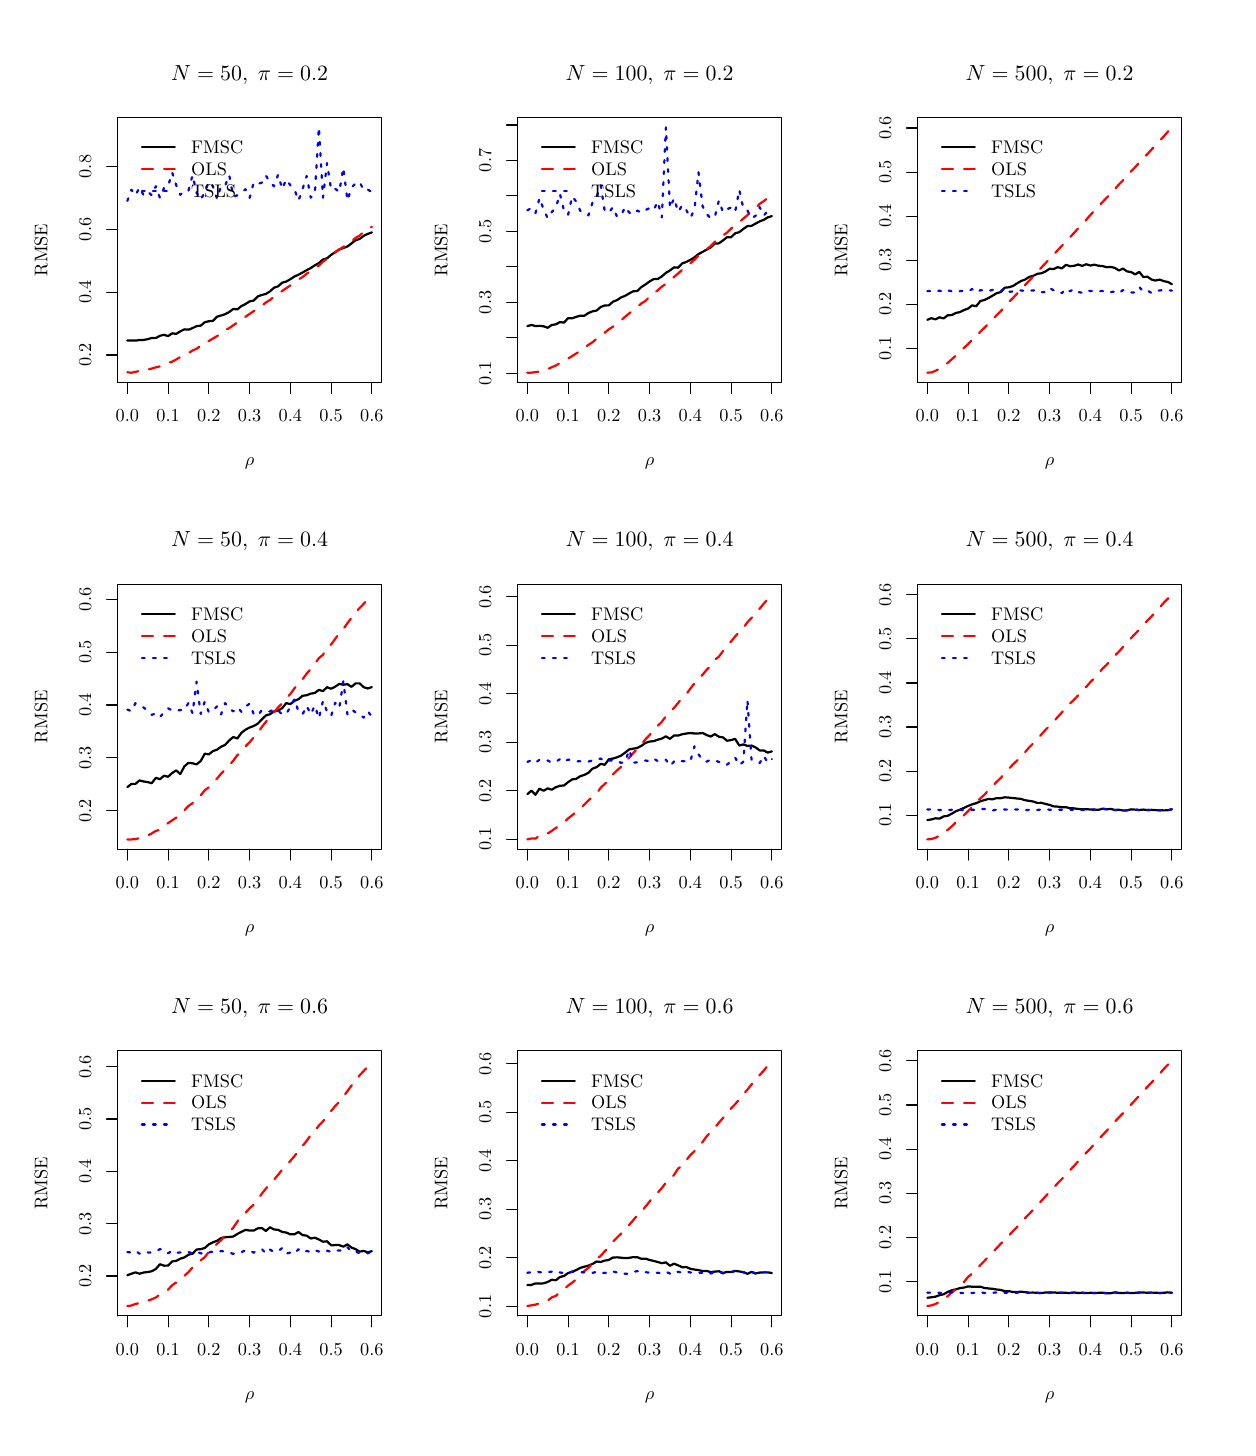
\begin{tikzpicture}[x=1pt,y=1pt]
\definecolor[named]{fillColor}{rgb}{1.00,1.00,1.00}
\path[use as bounding box,fill=fillColor,fill opacity=0.00] (0,0) rectangle (433.62,505.89);
\begin{scope}
\path[clip] ( 32.47,377.65) rectangle (127.91,473.42);
\definecolor[named]{drawColor}{rgb}{0.00,0.00,0.00}

\path[draw=drawColor,line width= 0.8pt,line join=round,line cap=round] ( 36.01,392.85) --
	( 37.48,392.85) --
	( 38.95,392.82) --
	( 40.42,392.99) --
	( 41.90,393.05) --
	( 43.37,393.32) --
	( 44.84,393.76) --
	( 46.32,393.73) --
	( 47.79,394.55) --
	( 49.26,394.91) --
	( 50.73,394.44) --
	( 52.21,395.44) --
	( 53.68,395.23) --
	( 55.15,396.16) --
	( 56.63,396.88) --
	( 58.10,396.76) --
	( 59.57,397.32) --
	( 61.04,398.05) --
	( 62.52,398.20) --
	( 63.99,399.44) --
	( 65.46,399.81) --
	( 66.93,399.94) --
	( 68.41,401.44) --
	( 69.88,401.88) --
	( 71.35,402.35) --
	( 72.83,403.14) --
	( 74.30,404.25) --
	( 75.77,404.09) --
	( 77.24,405.29) --
	( 78.72,406.02) --
	( 80.19,406.97) --
	( 81.66,407.27) --
	( 83.14,408.76) --
	( 84.61,409.31) --
	( 86.08,409.66) --
	( 87.55,410.59) --
	( 89.03,411.92) --
	( 90.50,412.42) --
	( 91.97,413.74) --
	( 93.44,414.14) --
	( 94.92,415.00) --
	( 96.39,415.97) --
	( 97.86,416.61) --
	( 99.34,417.42) --
	(100.81,418.25) --
	(102.28,419.03) --
	(103.75,420.01) --
	(105.23,420.82) --
	(106.70,422.09) --
	(108.17,422.54) --
	(109.65,423.80) --
	(111.12,424.77) --
	(112.59,425.70) --
	(114.06,426.28) --
	(115.54,426.81) --
	(117.01,427.93) --
	(118.48,429.07) --
	(119.95,429.54) --
	(121.43,430.66) --
	(122.90,431.38) --
	(124.37,431.90);
\end{scope}
\begin{scope}
\path[clip] (  0.00,  0.00) rectangle (433.62,505.89);
\definecolor[named]{drawColor}{rgb}{0.00,0.00,0.00}

\path[draw=drawColor,line width= 0.4pt,line join=round,line cap=round] ( 36.01,377.65) -- (124.37,377.65);

\path[draw=drawColor,line width= 0.4pt,line join=round,line cap=round] ( 36.01,377.65) -- ( 36.01,373.69);

\path[draw=drawColor,line width= 0.4pt,line join=round,line cap=round] ( 50.73,377.65) -- ( 50.73,373.69);

\path[draw=drawColor,line width= 0.4pt,line join=round,line cap=round] ( 65.46,377.65) -- ( 65.46,373.69);

\path[draw=drawColor,line width= 0.4pt,line join=round,line cap=round] ( 80.19,377.65) -- ( 80.19,373.69);

\path[draw=drawColor,line width= 0.4pt,line join=round,line cap=round] ( 94.92,377.65) -- ( 94.92,373.69);

\path[draw=drawColor,line width= 0.4pt,line join=round,line cap=round] (109.65,377.65) -- (109.65,373.69);

\path[draw=drawColor,line width= 0.4pt,line join=round,line cap=round] (124.37,377.65) -- (124.37,373.69);

\node[text=drawColor,anchor=base,inner sep=0pt, outer sep=0pt, scale=  0.66] at ( 36.01,363.40) {0.0};

\node[text=drawColor,anchor=base,inner sep=0pt, outer sep=0pt, scale=  0.66] at ( 50.73,363.40) {0.1};

\node[text=drawColor,anchor=base,inner sep=0pt, outer sep=0pt, scale=  0.66] at ( 65.46,363.40) {0.2};

\node[text=drawColor,anchor=base,inner sep=0pt, outer sep=0pt, scale=  0.66] at ( 80.19,363.40) {0.3};

\node[text=drawColor,anchor=base,inner sep=0pt, outer sep=0pt, scale=  0.66] at ( 94.92,363.40) {0.4};

\node[text=drawColor,anchor=base,inner sep=0pt, outer sep=0pt, scale=  0.66] at (109.65,363.40) {0.5};

\node[text=drawColor,anchor=base,inner sep=0pt, outer sep=0pt, scale=  0.66] at (124.37,363.40) {0.6};

\path[draw=drawColor,line width= 0.4pt,line join=round,line cap=round] ( 32.47,387.59) -- ( 32.47,455.73);

\path[draw=drawColor,line width= 0.4pt,line join=round,line cap=round] ( 32.47,387.59) -- ( 28.51,387.59);

\path[draw=drawColor,line width= 0.4pt,line join=round,line cap=round] ( 32.47,410.30) -- ( 28.51,410.30);

\path[draw=drawColor,line width= 0.4pt,line join=round,line cap=round] ( 32.47,433.02) -- ( 28.51,433.02);

\path[draw=drawColor,line width= 0.4pt,line join=round,line cap=round] ( 32.47,455.73) -- ( 28.51,455.73);

\node[text=drawColor,rotate= 90.00,anchor=base,inner sep=0pt, outer sep=0pt, scale=  0.66] at ( 22.97,387.59) {0.2};

\node[text=drawColor,rotate= 90.00,anchor=base,inner sep=0pt, outer sep=0pt, scale=  0.66] at ( 22.97,410.30) {0.4};

\node[text=drawColor,rotate= 90.00,anchor=base,inner sep=0pt, outer sep=0pt, scale=  0.66] at ( 22.97,433.02) {0.6};

\node[text=drawColor,rotate= 90.00,anchor=base,inner sep=0pt, outer sep=0pt, scale=  0.66] at ( 22.97,455.73) {0.8};

\path[draw=drawColor,line width= 0.4pt,line join=round,line cap=round] ( 32.47,377.65) --
	(127.91,377.65) --
	(127.91,473.42) --
	( 32.47,473.42) --
	( 32.47,377.65);
\end{scope}
\begin{scope}
\path[clip] (  0.00,337.26) rectangle (144.54,505.89);
\definecolor[named]{drawColor}{rgb}{0.00,0.00,0.00}

\node[text=drawColor,anchor=base,inner sep=0pt, outer sep=0pt, scale=  0.79] at ( 80.19,486.92) {\bfseries $N=50, \;\pi=0.2$};

\node[text=drawColor,anchor=base,inner sep=0pt, outer sep=0pt, scale=  0.66] at ( 80.19,347.56) {$\rho$};

\node[text=drawColor,rotate= 90.00,anchor=base,inner sep=0pt, outer sep=0pt, scale=  0.66] at (  7.13,425.53) {RMSE};
\end{scope}
\begin{scope}
\path[clip] ( 32.47,377.65) rectangle (127.91,473.42);
\definecolor[named]{drawColor}{rgb}{1.00,0.00,0.00}

\path[draw=drawColor,line width= 0.8pt,dash pattern=on 4pt off 4pt ,line join=round,line cap=round] ( 36.01,381.36) --
	( 37.48,381.20) --
	( 38.95,381.49) --
	( 40.42,381.86) --
	( 41.90,381.80) --
	( 43.37,382.32) --
	( 44.84,382.70) --
	( 46.32,383.15) --
	( 47.79,383.49) --
	( 49.26,384.27) --
	( 50.73,384.73) --
	( 52.21,385.20) --
	( 53.68,385.99) --
	( 55.15,386.88) --
	( 56.63,387.76) --
	( 58.10,388.30) --
	( 59.57,389.22) --
	( 61.04,389.85) --
	( 62.52,390.94) --
	( 63.99,392.08) --
	( 65.46,392.66) --
	( 66.93,393.54) --
	( 68.41,394.43) --
	( 69.88,395.21) --
	( 71.35,396.60) --
	( 72.83,397.31) --
	( 74.30,398.35) --
	( 75.77,399.35) --
	( 77.24,400.35) --
	( 78.72,401.43) --
	( 80.19,402.45) --
	( 81.66,403.45) --
	( 83.14,404.48) --
	( 84.61,405.41) --
	( 86.08,406.58) --
	( 87.55,407.49) --
	( 89.03,408.69) --
	( 90.50,409.35) --
	( 91.97,410.77) --
	( 93.44,411.75) --
	( 94.92,412.75) --
	( 96.39,414.06) --
	( 97.86,414.89) --
	( 99.34,415.77) --
	(100.81,416.98) --
	(102.28,417.93) --
	(103.75,419.08) --
	(105.23,419.91) --
	(106.70,421.31) --
	(108.17,422.34) --
	(109.65,423.54) --
	(111.12,424.75) --
	(112.59,425.76) --
	(114.06,426.67) --
	(115.54,427.66) --
	(117.01,428.70) --
	(118.48,429.92) --
	(119.95,430.74) --
	(121.43,432.08) --
	(122.90,433.23) --
	(124.37,433.92);
\definecolor[named]{drawColor}{rgb}{0.00,0.00,1.00}

\path[draw=drawColor,line width= 0.8pt,dash pattern=on 1pt off 3pt ,line join=round,line cap=round] ( 36.01,443.28) --
	( 37.48,447.36) --
	( 38.95,445.30) --
	( 40.42,448.16) --
	( 41.90,445.34) --
	( 43.37,446.58) --
	( 44.84,445.36) --
	( 46.32,448.60) --
	( 47.79,444.35) --
	( 49.26,447.89) --
	( 50.73,448.59) --
	( 52.21,453.56) --
	( 53.68,448.94) --
	( 55.15,445.48) --
	( 56.63,446.88) --
	( 58.10,446.98) --
	( 59.57,452.57) --
	( 61.04,446.27) --
	( 62.52,443.76) --
	( 63.99,446.35) --
	( 65.46,450.26) --
	( 66.93,448.68) --
	( 68.41,444.07) --
	( 69.88,448.63) --
	( 71.35,448.80) --
	( 72.83,452.57) --
	( 74.30,444.85) --
	( 75.77,445.31) --
	( 77.24,446.26) --
	( 78.72,447.50) --
	( 80.19,444.39) --
	( 81.66,449.87) --
	( 83.14,449.37) --
	( 84.61,449.91) --
	( 86.08,452.43) --
	( 87.55,450.07) --
	( 89.03,448.57) --
	( 90.50,452.79) --
	( 91.97,447.62) --
	( 93.44,451.06) --
	( 94.92,448.97) --
	( 96.39,447.49) --
	( 97.86,443.41) --
	( 99.34,447.60) --
	(100.81,452.30) --
	(102.28,444.47) --
	(103.75,445.83) --
	(105.23,469.87) --
	(106.70,444.43) --
	(108.17,456.95) --
	(109.65,447.37) --
	(111.12,447.67) --
	(112.59,446.52) --
	(114.06,455.25) --
	(115.54,443.48) --
	(117.01,448.03) --
	(118.48,449.65) --
	(119.95,450.13) --
	(121.43,447.14) --
	(122.90,447.40) --
	(124.37,446.42);
\definecolor[named]{drawColor}{rgb}{0.00,0.00,0.00}

\path[draw=drawColor,line width= 0.8pt,line join=round,line cap=round] ( 41.28,462.63) -- ( 53.16,462.63);
\definecolor[named]{drawColor}{rgb}{1.00,0.00,0.00}

\path[draw=drawColor,line width= 0.8pt,dash pattern=on 4pt off 4pt ,line join=round,line cap=round] ( 41.28,454.71) -- ( 53.16,454.71);
\definecolor[named]{drawColor}{rgb}{0.00,0.00,1.00}

\path[draw=drawColor,line width= 0.8pt,dash pattern=on 1pt off 3pt ,line join=round,line cap=round] ( 41.28,446.79) -- ( 53.16,446.79);
\definecolor[named]{drawColor}{rgb}{0.00,0.00,0.00}

\node[text=drawColor,anchor=base west,inner sep=0pt, outer sep=0pt, scale=  0.66] at ( 59.10,460.35) {FMSC};

\node[text=drawColor,anchor=base west,inner sep=0pt, outer sep=0pt, scale=  0.66] at ( 59.10,452.43) {OLS};

\node[text=drawColor,anchor=base west,inner sep=0pt, outer sep=0pt, scale=  0.66] at ( 59.10,444.51) {TSLS};
\end{scope}
\begin{scope}
\path[clip] (177.01,377.65) rectangle (272.45,473.42);
\definecolor[named]{drawColor}{rgb}{0.00,0.00,0.00}

\path[draw=drawColor,line width= 0.8pt,line join=round,line cap=round] (180.55,398.03) --
	(182.02,398.46) --
	(183.49,398.06) --
	(184.96,398.14) --
	(186.44,397.98) --
	(187.91,397.44) --
	(189.38,398.43) --
	(190.86,398.70) --
	(192.33,399.49) --
	(193.80,399.31) --
	(195.27,400.93) --
	(196.75,400.85) --
	(198.22,401.40) --
	(199.69,401.82) --
	(201.17,401.81) --
	(202.64,402.79) --
	(204.11,403.39) --
	(205.58,403.67) --
	(207.06,404.95) --
	(208.53,405.52) --
	(210.00,405.54) --
	(211.47,406.84) --
	(212.95,407.43) --
	(214.42,408.41) --
	(215.89,408.99) --
	(217.37,409.86) --
	(218.84,410.64) --
	(220.31,410.73) --
	(221.78,412.18) --
	(223.26,413.11) --
	(224.73,414.19) --
	(226.20,415.02) --
	(227.68,415.05) --
	(229.15,416.01) --
	(230.62,417.28) --
	(232.09,418.15) --
	(233.57,419.28) --
	(235.04,419.15) --
	(236.51,420.70) --
	(237.98,421.22) --
	(239.46,421.97) --
	(240.93,422.89) --
	(242.40,424.07) --
	(243.88,424.87) --
	(245.35,425.66) --
	(246.82,426.49) --
	(248.29,427.85) --
	(249.77,427.95) --
	(251.24,429.01) --
	(252.71,430.15) --
	(254.19,430.17) --
	(255.66,431.59) --
	(257.13,431.99) --
	(258.60,433.15) --
	(260.08,434.19) --
	(261.55,434.26) --
	(263.02,435.08) --
	(264.50,435.88) --
	(265.97,436.45) --
	(267.44,437.33) --
	(268.91,437.78);
\end{scope}
\begin{scope}
\path[clip] (  0.00,  0.00) rectangle (433.62,505.89);
\definecolor[named]{drawColor}{rgb}{0.00,0.00,0.00}

\path[draw=drawColor,line width= 0.4pt,line join=round,line cap=round] (180.55,377.65) -- (268.91,377.65);

\path[draw=drawColor,line width= 0.4pt,line join=round,line cap=round] (180.55,377.65) -- (180.55,373.69);

\path[draw=drawColor,line width= 0.4pt,line join=round,line cap=round] (195.27,377.65) -- (195.27,373.69);

\path[draw=drawColor,line width= 0.4pt,line join=round,line cap=round] (210.00,377.65) -- (210.00,373.69);

\path[draw=drawColor,line width= 0.4pt,line join=round,line cap=round] (224.73,377.65) -- (224.73,373.69);

\path[draw=drawColor,line width= 0.4pt,line join=round,line cap=round] (239.46,377.65) -- (239.46,373.69);

\path[draw=drawColor,line width= 0.4pt,line join=round,line cap=round] (254.19,377.65) -- (254.19,373.69);

\path[draw=drawColor,line width= 0.4pt,line join=round,line cap=round] (268.91,377.65) -- (268.91,373.69);

\node[text=drawColor,anchor=base,inner sep=0pt, outer sep=0pt, scale=  0.66] at (180.55,363.40) {0.0};

\node[text=drawColor,anchor=base,inner sep=0pt, outer sep=0pt, scale=  0.66] at (195.27,363.40) {0.1};

\node[text=drawColor,anchor=base,inner sep=0pt, outer sep=0pt, scale=  0.66] at (210.00,363.40) {0.2};

\node[text=drawColor,anchor=base,inner sep=0pt, outer sep=0pt, scale=  0.66] at (224.73,363.40) {0.3};

\node[text=drawColor,anchor=base,inner sep=0pt, outer sep=0pt, scale=  0.66] at (239.46,363.40) {0.4};

\node[text=drawColor,anchor=base,inner sep=0pt, outer sep=0pt, scale=  0.66] at (254.19,363.40) {0.5};

\node[text=drawColor,anchor=base,inner sep=0pt, outer sep=0pt, scale=  0.66] at (268.91,363.40) {0.6};

\path[draw=drawColor,line width= 0.4pt,line join=round,line cap=round] (177.01,380.98) -- (177.01,470.73);

\path[draw=drawColor,line width= 0.4pt,line join=round,line cap=round] (177.01,380.98) -- (173.05,380.98);

\path[draw=drawColor,line width= 0.4pt,line join=round,line cap=round] (177.01,393.81) -- (173.05,393.81);

\path[draw=drawColor,line width= 0.4pt,line join=round,line cap=round] (177.01,406.63) -- (173.05,406.63);

\path[draw=drawColor,line width= 0.4pt,line join=round,line cap=round] (177.01,419.45) -- (173.05,419.45);

\path[draw=drawColor,line width= 0.4pt,line join=round,line cap=round] (177.01,432.27) -- (173.05,432.27);

\path[draw=drawColor,line width= 0.4pt,line join=round,line cap=round] (177.01,445.09) -- (173.05,445.09);

\path[draw=drawColor,line width= 0.4pt,line join=round,line cap=round] (177.01,457.91) -- (173.05,457.91);

\path[draw=drawColor,line width= 0.4pt,line join=round,line cap=round] (177.01,470.73) -- (173.05,470.73);

\node[text=drawColor,rotate= 90.00,anchor=base,inner sep=0pt, outer sep=0pt, scale=  0.66] at (167.51,380.98) {0.1};

\node[text=drawColor,rotate= 90.00,anchor=base,inner sep=0pt, outer sep=0pt, scale=  0.66] at (167.51,406.63) {0.3};

\node[text=drawColor,rotate= 90.00,anchor=base,inner sep=0pt, outer sep=0pt, scale=  0.66] at (167.51,432.27) {0.5};

\node[text=drawColor,rotate= 90.00,anchor=base,inner sep=0pt, outer sep=0pt, scale=  0.66] at (167.51,457.91) {0.7};

\path[draw=drawColor,line width= 0.4pt,line join=round,line cap=round] (177.01,377.65) --
	(272.45,377.65) --
	(272.45,473.42) --
	(177.01,473.42) --
	(177.01,377.65);
\end{scope}
\begin{scope}
\path[clip] (144.54,337.26) rectangle (289.08,505.89);
\definecolor[named]{drawColor}{rgb}{0.00,0.00,0.00}

\node[text=drawColor,anchor=base,inner sep=0pt, outer sep=0pt, scale=  0.79] at (224.73,486.92) {\bfseries $N=100, \;\pi=0.2$};

\node[text=drawColor,anchor=base,inner sep=0pt, outer sep=0pt, scale=  0.66] at (224.73,347.56) {$\rho$};

\node[text=drawColor,rotate= 90.00,anchor=base,inner sep=0pt, outer sep=0pt, scale=  0.66] at (151.67,425.53) {RMSE};
\end{scope}
\begin{scope}
\path[clip] (177.01,377.65) rectangle (272.45,473.42);
\definecolor[named]{drawColor}{rgb}{1.00,0.00,0.00}

\path[draw=drawColor,line width= 0.8pt,dash pattern=on 4pt off 4pt ,line join=round,line cap=round] (180.55,381.20) --
	(182.02,381.23) --
	(183.49,381.43) --
	(184.96,381.60) --
	(186.44,382.23) --
	(187.91,382.50) --
	(189.38,383.19) --
	(190.86,383.79) --
	(192.33,384.67) --
	(193.80,385.59) --
	(195.27,386.31) --
	(196.75,387.22) --
	(198.22,388.17) --
	(199.69,389.13) --
	(201.17,390.25) --
	(202.64,391.29) --
	(204.11,392.22) --
	(205.58,393.47) --
	(207.06,394.73) --
	(208.53,395.67) --
	(210.00,396.91) --
	(211.47,397.81) --
	(212.95,398.99) --
	(214.42,400.12) --
	(215.89,401.44) --
	(217.37,402.65) --
	(218.84,403.80) --
	(220.31,404.91) --
	(221.78,406.26) --
	(223.26,407.17) --
	(224.73,408.69) --
	(226.20,409.91) --
	(227.68,410.98) --
	(229.15,412.30) --
	(230.62,413.35) --
	(232.09,414.48) --
	(233.57,415.81) --
	(235.04,417.05) --
	(236.51,418.43) --
	(237.98,419.47) --
	(239.46,420.74) --
	(240.93,422.00) --
	(242.40,423.55) --
	(243.88,424.51) --
	(245.35,425.79) --
	(246.82,426.96) --
	(248.29,428.47) --
	(249.77,429.76) --
	(251.24,430.77) --
	(252.71,431.84) --
	(254.19,433.27) --
	(255.66,434.50) --
	(257.13,435.65) --
	(258.60,436.89) --
	(260.08,438.13) --
	(261.55,439.44) --
	(263.02,440.65) --
	(264.50,442.23) --
	(265.97,443.19) --
	(267.44,444.40) --
	(268.91,445.81);
\definecolor[named]{drawColor}{rgb}{0.00,0.00,1.00}

\path[draw=drawColor,line width= 0.8pt,dash pattern=on 1pt off 3pt ,line join=round,line cap=round] (180.55,439.89) --
	(182.02,440.70) --
	(183.49,438.88) --
	(184.96,444.31) --
	(186.44,440.13) --
	(187.91,437.02) --
	(189.38,439.27) --
	(190.86,440.83) --
	(192.33,445.84) --
	(193.80,439.78) --
	(195.27,438.23) --
	(196.75,444.94) --
	(198.22,443.00) --
	(199.69,439.70) --
	(201.17,438.86) --
	(202.64,438.08) --
	(204.11,442.72) --
	(205.58,444.83) --
	(207.06,448.91) --
	(208.53,439.53) --
	(210.00,439.08) --
	(211.47,441.01) --
	(212.95,437.61) --
	(214.42,438.03) --
	(215.89,441.14) --
	(217.37,439.06) --
	(218.84,438.46) --
	(220.31,439.78) --
	(221.78,438.99) --
	(223.26,439.97) --
	(224.73,440.74) --
	(226.20,440.01) --
	(227.68,443.04) --
	(229.15,437.32) --
	(230.62,469.87) --
	(232.09,440.76) --
	(233.57,444.22) --
	(235.04,439.32) --
	(236.51,441.70) --
	(237.98,440.02) --
	(239.46,437.16) --
	(240.93,440.15) --
	(242.40,453.61) --
	(243.88,441.36) --
	(245.35,438.49) --
	(246.82,437.01) --
	(248.29,437.50) --
	(249.77,443.43) --
	(251.24,439.20) --
	(252.71,440.30) --
	(254.19,440.89) --
	(255.66,439.36) --
	(257.13,447.31) --
	(258.60,440.58) --
	(260.08,439.80) --
	(261.55,437.08) --
	(263.02,437.87) --
	(264.50,441.05) --
	(265.97,438.01) --
	(267.44,439.66) --
	(268.91,441.06);
\definecolor[named]{drawColor}{rgb}{0.00,0.00,0.00}

\path[draw=drawColor,line width= 0.8pt,line join=round,line cap=round] (185.82,462.63) -- (197.70,462.63);
\definecolor[named]{drawColor}{rgb}{1.00,0.00,0.00}

\path[draw=drawColor,line width= 0.8pt,dash pattern=on 4pt off 4pt ,line join=round,line cap=round] (185.82,454.71) -- (197.70,454.71);
\definecolor[named]{drawColor}{rgb}{0.00,0.00,1.00}

\path[draw=drawColor,line width= 0.8pt,dash pattern=on 1pt off 3pt ,line join=round,line cap=round] (185.82,446.79) -- (197.70,446.79);
\definecolor[named]{drawColor}{rgb}{0.00,0.00,0.00}

\node[text=drawColor,anchor=base west,inner sep=0pt, outer sep=0pt, scale=  0.66] at (203.64,460.35) {FMSC};

\node[text=drawColor,anchor=base west,inner sep=0pt, outer sep=0pt, scale=  0.66] at (203.64,452.43) {OLS};

\node[text=drawColor,anchor=base west,inner sep=0pt, outer sep=0pt, scale=  0.66] at (203.64,444.51) {TSLS};
\end{scope}
\begin{scope}
\path[clip] (321.55,377.65) rectangle (416.99,473.42);
\definecolor[named]{drawColor}{rgb}{0.00,0.00,0.00}

\path[draw=drawColor,line width= 0.8pt,line join=round,line cap=round] (325.09,400.32) --
	(326.56,400.91) --
	(328.03,400.48) --
	(329.50,401.23) --
	(330.98,400.82) --
	(332.45,401.95) --
	(333.92,402.04) --
	(335.40,402.79) --
	(336.87,403.13) --
	(338.34,403.85) --
	(339.81,404.38) --
	(341.29,405.54) --
	(342.76,405.24) --
	(344.23,407.08) --
	(345.71,407.50) --
	(347.18,408.19) --
	(348.65,409.05) --
	(350.12,409.93) --
	(351.60,410.34) --
	(353.07,411.93) --
	(354.54,412.07) --
	(356.01,412.52) --
	(357.49,413.48) --
	(358.96,414.34) --
	(360.43,414.88) --
	(361.91,415.84) --
	(363.38,416.21) --
	(364.85,416.94) --
	(366.32,417.15) --
	(367.80,417.79) --
	(369.27,418.77) --
	(370.74,418.66) --
	(372.22,419.36) --
	(373.69,418.90) --
	(375.16,420.17) --
	(376.63,419.69) --
	(378.11,419.81) --
	(379.58,420.31) --
	(381.05,419.81) --
	(382.52,420.39) --
	(384.00,419.94) --
	(385.47,420.24) --
	(386.94,419.86) --
	(388.42,419.73) --
	(389.89,419.34) --
	(391.36,419.41) --
	(392.83,419.09) --
	(394.31,418.14) --
	(395.78,418.82) --
	(397.25,417.82) --
	(398.73,417.57) --
	(400.20,416.75) --
	(401.67,417.63) --
	(403.14,415.78) --
	(404.62,415.89) --
	(406.09,414.88) --
	(407.56,414.51) --
	(409.04,414.86) --
	(410.51,414.30) --
	(411.98,414.00) --
	(413.45,413.21);
\end{scope}
\begin{scope}
\path[clip] (  0.00,  0.00) rectangle (433.62,505.89);
\definecolor[named]{drawColor}{rgb}{0.00,0.00,0.00}

\path[draw=drawColor,line width= 0.4pt,line join=round,line cap=round] (325.09,377.65) -- (413.45,377.65);

\path[draw=drawColor,line width= 0.4pt,line join=round,line cap=round] (325.09,377.65) -- (325.09,373.69);

\path[draw=drawColor,line width= 0.4pt,line join=round,line cap=round] (339.81,377.65) -- (339.81,373.69);

\path[draw=drawColor,line width= 0.4pt,line join=round,line cap=round] (354.54,377.65) -- (354.54,373.69);

\path[draw=drawColor,line width= 0.4pt,line join=round,line cap=round] (369.27,377.65) -- (369.27,373.69);

\path[draw=drawColor,line width= 0.4pt,line join=round,line cap=round] (384.00,377.65) -- (384.00,373.69);

\path[draw=drawColor,line width= 0.4pt,line join=round,line cap=round] (398.73,377.65) -- (398.73,373.69);

\path[draw=drawColor,line width= 0.4pt,line join=round,line cap=round] (413.45,377.65) -- (413.45,373.69);

\node[text=drawColor,anchor=base,inner sep=0pt, outer sep=0pt, scale=  0.66] at (325.09,363.40) {0.0};

\node[text=drawColor,anchor=base,inner sep=0pt, outer sep=0pt, scale=  0.66] at (339.81,363.40) {0.1};

\node[text=drawColor,anchor=base,inner sep=0pt, outer sep=0pt, scale=  0.66] at (354.54,363.40) {0.2};

\node[text=drawColor,anchor=base,inner sep=0pt, outer sep=0pt, scale=  0.66] at (369.27,363.40) {0.3};

\node[text=drawColor,anchor=base,inner sep=0pt, outer sep=0pt, scale=  0.66] at (384.00,363.40) {0.4};

\node[text=drawColor,anchor=base,inner sep=0pt, outer sep=0pt, scale=  0.66] at (398.73,363.40) {0.5};

\node[text=drawColor,anchor=base,inner sep=0pt, outer sep=0pt, scale=  0.66] at (413.45,363.40) {0.6};

\path[draw=drawColor,line width= 0.4pt,line join=round,line cap=round] (321.55,389.99) -- (321.55,469.62);

\path[draw=drawColor,line width= 0.4pt,line join=round,line cap=round] (321.55,389.99) -- (317.59,389.99);

\path[draw=drawColor,line width= 0.4pt,line join=round,line cap=round] (321.55,405.92) -- (317.59,405.92);

\path[draw=drawColor,line width= 0.4pt,line join=round,line cap=round] (321.55,421.84) -- (317.59,421.84);

\path[draw=drawColor,line width= 0.4pt,line join=round,line cap=round] (321.55,437.77) -- (317.59,437.77);

\path[draw=drawColor,line width= 0.4pt,line join=round,line cap=round] (321.55,453.69) -- (317.59,453.69);

\path[draw=drawColor,line width= 0.4pt,line join=round,line cap=round] (321.55,469.62) -- (317.59,469.62);

\node[text=drawColor,rotate= 90.00,anchor=base,inner sep=0pt, outer sep=0pt, scale=  0.66] at (312.05,389.99) {0.1};

\node[text=drawColor,rotate= 90.00,anchor=base,inner sep=0pt, outer sep=0pt, scale=  0.66] at (312.05,405.92) {0.2};

\node[text=drawColor,rotate= 90.00,anchor=base,inner sep=0pt, outer sep=0pt, scale=  0.66] at (312.05,421.84) {0.3};

\node[text=drawColor,rotate= 90.00,anchor=base,inner sep=0pt, outer sep=0pt, scale=  0.66] at (312.05,437.77) {0.4};

\node[text=drawColor,rotate= 90.00,anchor=base,inner sep=0pt, outer sep=0pt, scale=  0.66] at (312.05,453.69) {0.5};

\node[text=drawColor,rotate= 90.00,anchor=base,inner sep=0pt, outer sep=0pt, scale=  0.66] at (312.05,469.62) {0.6};

\path[draw=drawColor,line width= 0.4pt,line join=round,line cap=round] (321.55,377.65) --
	(416.99,377.65) --
	(416.99,473.42) --
	(321.55,473.42) --
	(321.55,377.65);
\end{scope}
\begin{scope}
\path[clip] (289.08,337.26) rectangle (433.62,505.89);
\definecolor[named]{drawColor}{rgb}{0.00,0.00,0.00}

\node[text=drawColor,anchor=base,inner sep=0pt, outer sep=0pt, scale=  0.79] at (369.27,486.92) {\bfseries $N=500, \;\pi=0.2$};

\node[text=drawColor,anchor=base,inner sep=0pt, outer sep=0pt, scale=  0.66] at (369.27,347.56) {$\rho$};

\node[text=drawColor,rotate= 90.00,anchor=base,inner sep=0pt, outer sep=0pt, scale=  0.66] at (296.21,425.53) {RMSE};
\end{scope}
\begin{scope}
\path[clip] (321.55,377.65) rectangle (416.99,473.42);
\definecolor[named]{drawColor}{rgb}{1.00,0.00,0.00}

\path[draw=drawColor,line width= 0.8pt,dash pattern=on 4pt off 4pt ,line join=round,line cap=round] (325.09,381.20) --
	(326.56,381.32) --
	(328.03,381.88) --
	(329.50,382.60) --
	(330.98,383.66) --
	(332.45,384.74) --
	(333.92,386.04) --
	(335.40,387.39) --
	(336.87,388.72) --
	(338.34,390.20) --
	(339.81,391.50) --
	(341.29,393.13) --
	(342.76,394.39) --
	(344.23,395.98) --
	(345.71,397.43) --
	(347.18,398.91) --
	(348.65,400.51) --
	(350.12,401.97) --
	(351.60,403.46) --
	(353.07,405.09) --
	(354.54,406.74) --
	(356.01,408.17) --
	(357.49,409.76) --
	(358.96,411.42) --
	(360.43,412.92) --
	(361.91,414.48) --
	(363.38,416.01) --
	(364.85,417.61) --
	(366.32,419.23) --
	(367.80,420.81) --
	(369.27,422.33) --
	(370.74,423.89) --
	(372.22,425.49) --
	(373.69,427.07) --
	(375.16,428.64) --
	(376.63,430.12) --
	(378.11,431.74) --
	(379.58,433.37) --
	(381.05,434.98) --
	(382.52,436.48) --
	(384.00,438.20) --
	(385.47,439.75) --
	(386.94,441.32) --
	(388.42,442.88) --
	(389.89,444.45) --
	(391.36,445.93) --
	(392.83,447.58) --
	(394.31,449.20) --
	(395.78,450.71) --
	(397.25,452.45) --
	(398.73,453.99) --
	(400.20,455.46) --
	(401.67,457.17) --
	(403.14,458.68) --
	(404.62,460.21) --
	(406.09,461.83) --
	(407.56,463.43) --
	(409.04,465.02) --
	(410.51,466.57) --
	(411.98,468.27) --
	(413.45,469.87);
\definecolor[named]{drawColor}{rgb}{0.00,0.00,1.00}

\path[draw=drawColor,line width= 0.8pt,dash pattern=on 1pt off 3pt ,line join=round,line cap=round] (325.09,410.68) --
	(326.56,410.73) --
	(328.03,410.53) --
	(329.50,410.86) --
	(330.98,410.35) --
	(332.45,410.97) --
	(333.92,410.62) --
	(335.40,410.83) --
	(336.87,410.67) --
	(338.34,410.84) --
	(339.81,410.62) --
	(341.29,411.42) --
	(342.76,410.19) --
	(344.23,411.01) --
	(345.71,411.03) --
	(347.18,410.73) --
	(348.65,411.14) --
	(350.12,411.01) --
	(351.60,410.63) --
	(353.07,411.81) --
	(354.54,410.46) --
	(356.01,410.54) --
	(357.49,410.98) --
	(358.96,410.95) --
	(360.43,410.70) --
	(361.91,410.85) --
	(363.38,410.93) --
	(364.85,411.12) --
	(366.32,410.29) --
	(367.80,410.38) --
	(369.27,411.78) --
	(370.74,410.97) --
	(372.22,410.87) --
	(373.69,409.95) --
	(375.16,411.62) --
	(376.63,410.63) --
	(378.11,411.43) --
	(379.58,410.37) --
	(381.05,410.09) --
	(382.52,410.92) --
	(384.00,410.73) --
	(385.47,410.78) --
	(386.94,410.62) --
	(388.42,410.76) --
	(389.89,410.21) --
	(391.36,410.37) --
	(392.83,410.50) --
	(394.31,409.92) --
	(395.78,411.05) --
	(397.25,410.83) --
	(398.73,410.22) --
	(400.20,410.18) --
	(401.67,412.12) --
	(403.14,410.57) --
	(404.62,410.92) --
	(406.09,410.02) --
	(407.56,410.69) --
	(409.04,410.93) --
	(410.51,411.07) --
	(411.98,411.06) --
	(413.45,410.87);
\definecolor[named]{drawColor}{rgb}{0.00,0.00,0.00}

\path[draw=drawColor,line width= 0.8pt,line join=round,line cap=round] (330.36,462.63) -- (342.24,462.63);
\definecolor[named]{drawColor}{rgb}{1.00,0.00,0.00}

\path[draw=drawColor,line width= 0.8pt,dash pattern=on 4pt off 4pt ,line join=round,line cap=round] (330.36,454.71) -- (342.24,454.71);
\definecolor[named]{drawColor}{rgb}{0.00,0.00,1.00}

\path[draw=drawColor,line width= 0.8pt,dash pattern=on 1pt off 3pt ,line join=round,line cap=round] (330.36,446.79) -- (342.24,446.79);
\definecolor[named]{drawColor}{rgb}{0.00,0.00,0.00}

\node[text=drawColor,anchor=base west,inner sep=0pt, outer sep=0pt, scale=  0.66] at (348.18,460.35) {FMSC};

\node[text=drawColor,anchor=base west,inner sep=0pt, outer sep=0pt, scale=  0.66] at (348.18,452.43) {OLS};

\node[text=drawColor,anchor=base west,inner sep=0pt, outer sep=0pt, scale=  0.66] at (348.18,444.51) {TSLS};
\end{scope}
\begin{scope}
\path[clip] ( 32.47,209.02) rectangle (127.91,304.79);
\definecolor[named]{drawColor}{rgb}{0.00,0.00,0.00}

\path[draw=drawColor,line width= 0.8pt,line join=round,line cap=round] ( 36.01,231.45) --
	( 37.48,232.62) --
	( 38.95,232.64) --
	( 40.42,233.88) --
	( 41.90,233.50) --
	( 43.37,233.27) --
	( 44.84,232.88) --
	( 46.32,234.83) --
	( 47.79,234.32) --
	( 49.26,235.57) --
	( 50.73,235.20) --
	( 52.21,236.56) --
	( 53.68,237.51) --
	( 55.15,236.18) --
	( 56.63,238.97) --
	( 58.10,240.23) --
	( 59.57,240.07) --
	( 61.04,239.68) --
	( 62.52,240.86) --
	( 63.99,243.54) --
	( 65.46,243.30) --
	( 66.93,244.48) --
	( 68.41,244.99) --
	( 69.88,246.05) --
	( 71.35,246.72) --
	( 72.83,248.34) --
	( 74.30,249.56) --
	( 75.77,249.04) --
	( 77.24,251.08) --
	( 78.72,252.21) --
	( 80.19,253.00) --
	( 81.66,253.54) --
	( 83.14,254.40) --
	( 84.61,255.93) --
	( 86.08,257.36) --
	( 87.55,257.80) --
	( 89.03,258.84) --
	( 90.50,259.14) --
	( 91.97,259.98) --
	( 93.44,261.84) --
	( 94.92,261.43) --
	( 96.39,262.63) --
	( 97.86,263.25) --
	( 99.34,264.47) --
	(100.81,264.66) --
	(102.28,265.24) --
	(103.75,265.48) --
	(105.23,266.59) --
	(106.70,266.16) --
	(108.17,267.55) --
	(109.65,267.02) --
	(111.12,267.76) --
	(112.59,268.74) --
	(114.06,268.47) --
	(115.54,268.66) --
	(117.01,267.69) --
	(118.48,268.95) --
	(119.95,268.95) --
	(121.43,267.56) --
	(122.90,267.11) --
	(124.37,267.59);
\end{scope}
\begin{scope}
\path[clip] (  0.00,  0.00) rectangle (433.62,505.89);
\definecolor[named]{drawColor}{rgb}{0.00,0.00,0.00}

\path[draw=drawColor,line width= 0.4pt,line join=round,line cap=round] ( 36.01,209.02) -- (124.37,209.02);

\path[draw=drawColor,line width= 0.4pt,line join=round,line cap=round] ( 36.01,209.02) -- ( 36.01,205.06);

\path[draw=drawColor,line width= 0.4pt,line join=round,line cap=round] ( 50.73,209.02) -- ( 50.73,205.06);

\path[draw=drawColor,line width= 0.4pt,line join=round,line cap=round] ( 65.46,209.02) -- ( 65.46,205.06);

\path[draw=drawColor,line width= 0.4pt,line join=round,line cap=round] ( 80.19,209.02) -- ( 80.19,205.06);

\path[draw=drawColor,line width= 0.4pt,line join=round,line cap=round] ( 94.92,209.02) -- ( 94.92,205.06);

\path[draw=drawColor,line width= 0.4pt,line join=round,line cap=round] (109.65,209.02) -- (109.65,205.06);

\path[draw=drawColor,line width= 0.4pt,line join=round,line cap=round] (124.37,209.02) -- (124.37,205.06);

\node[text=drawColor,anchor=base,inner sep=0pt, outer sep=0pt, scale=  0.66] at ( 36.01,194.77) {0.0};

\node[text=drawColor,anchor=base,inner sep=0pt, outer sep=0pt, scale=  0.66] at ( 50.73,194.77) {0.1};

\node[text=drawColor,anchor=base,inner sep=0pt, outer sep=0pt, scale=  0.66] at ( 65.46,194.77) {0.2};

\node[text=drawColor,anchor=base,inner sep=0pt, outer sep=0pt, scale=  0.66] at ( 80.19,194.77) {0.3};

\node[text=drawColor,anchor=base,inner sep=0pt, outer sep=0pt, scale=  0.66] at ( 94.92,194.77) {0.4};

\node[text=drawColor,anchor=base,inner sep=0pt, outer sep=0pt, scale=  0.66] at (109.65,194.77) {0.5};

\node[text=drawColor,anchor=base,inner sep=0pt, outer sep=0pt, scale=  0.66] at (124.37,194.77) {0.6};

\path[draw=drawColor,line width= 0.4pt,line join=round,line cap=round] ( 32.47,222.99) -- ( 32.47,299.31);

\path[draw=drawColor,line width= 0.4pt,line join=round,line cap=round] ( 32.47,222.99) -- ( 28.51,222.99);

\path[draw=drawColor,line width= 0.4pt,line join=round,line cap=round] ( 32.47,242.07) -- ( 28.51,242.07);

\path[draw=drawColor,line width= 0.4pt,line join=round,line cap=round] ( 32.47,261.15) -- ( 28.51,261.15);

\path[draw=drawColor,line width= 0.4pt,line join=round,line cap=round] ( 32.47,280.23) -- ( 28.51,280.23);

\path[draw=drawColor,line width= 0.4pt,line join=round,line cap=round] ( 32.47,299.31) -- ( 28.51,299.31);

\node[text=drawColor,rotate= 90.00,anchor=base,inner sep=0pt, outer sep=0pt, scale=  0.66] at ( 22.97,222.99) {0.2};

\node[text=drawColor,rotate= 90.00,anchor=base,inner sep=0pt, outer sep=0pt, scale=  0.66] at ( 22.97,242.07) {0.3};

\node[text=drawColor,rotate= 90.00,anchor=base,inner sep=0pt, outer sep=0pt, scale=  0.66] at ( 22.97,261.15) {0.4};

\node[text=drawColor,rotate= 90.00,anchor=base,inner sep=0pt, outer sep=0pt, scale=  0.66] at ( 22.97,280.23) {0.5};

\node[text=drawColor,rotate= 90.00,anchor=base,inner sep=0pt, outer sep=0pt, scale=  0.66] at ( 22.97,299.31) {0.6};

\path[draw=drawColor,line width= 0.4pt,line join=round,line cap=round] ( 32.47,209.02) --
	(127.91,209.02) --
	(127.91,304.79) --
	( 32.47,304.79) --
	( 32.47,209.02);
\end{scope}
\begin{scope}
\path[clip] (  0.00,168.63) rectangle (144.54,337.26);
\definecolor[named]{drawColor}{rgb}{0.00,0.00,0.00}

\node[text=drawColor,anchor=base,inner sep=0pt, outer sep=0pt, scale=  0.79] at ( 80.19,318.29) {\bfseries $N=50, \;\pi=0.4$};

\node[text=drawColor,anchor=base,inner sep=0pt, outer sep=0pt, scale=  0.66] at ( 80.19,178.93) {$\rho$};

\node[text=drawColor,rotate= 90.00,anchor=base,inner sep=0pt, outer sep=0pt, scale=  0.66] at (  7.13,256.90) {RMSE};
\end{scope}
\begin{scope}
\path[clip] ( 32.47,209.02) rectangle (127.91,304.79);
\definecolor[named]{drawColor}{rgb}{1.00,0.00,0.00}

\path[draw=drawColor,line width= 0.8pt,dash pattern=on 4pt off 4pt ,line join=round,line cap=round] ( 36.01,212.57) --
	( 37.48,212.57) --
	( 38.95,212.66) --
	( 40.42,213.06) --
	( 41.90,213.25) --
	( 43.37,213.95) --
	( 44.84,214.74) --
	( 46.32,215.64) --
	( 47.79,216.04) --
	( 49.26,217.31) --
	( 50.73,218.45) --
	( 52.21,219.44) --
	( 53.68,220.42) --
	( 55.15,221.39) --
	( 56.63,223.10) --
	( 58.10,224.64) --
	( 59.57,225.67) --
	( 61.04,226.93) --
	( 62.52,228.51) --
	( 63.99,230.28) --
	( 65.46,231.42) --
	( 66.93,233.17) --
	( 68.41,234.53) --
	( 69.88,236.32) --
	( 71.35,237.78) --
	( 72.83,239.36) --
	( 74.30,241.03) --
	( 75.77,243.02) --
	( 77.24,244.61) --
	( 78.72,246.24) --
	( 80.19,247.67) --
	( 81.66,249.43) --
	( 83.14,250.98) --
	( 84.61,253.17) --
	( 86.08,255.06) --
	( 87.55,256.58) --
	( 89.03,258.51) --
	( 90.50,260.26) --
	( 91.97,261.76) --
	( 93.44,263.60) --
	( 94.92,265.11) --
	( 96.39,267.16) --
	( 97.86,268.97) --
	( 99.34,270.44) --
	(100.81,272.45) --
	(102.28,274.13) --
	(103.75,275.99) --
	(105.23,278.07) --
	(106.70,279.26) --
	(108.17,281.94) --
	(109.65,283.01) --
	(111.12,285.02) --
	(112.59,287.13) --
	(114.06,288.58) --
	(115.54,290.70) --
	(117.01,292.61) --
	(118.48,294.70) --
	(119.95,296.20) --
	(121.43,297.69) --
	(122.90,299.35) --
	(124.37,301.24);
\definecolor[named]{drawColor}{rgb}{0.00,0.00,1.00}

\path[draw=drawColor,line width= 0.8pt,dash pattern=on 1pt off 3pt ,line join=round,line cap=round] ( 36.01,259.50) --
	( 37.48,258.88) --
	( 38.95,261.78) --
	( 40.42,260.84) --
	( 41.90,260.23) --
	( 43.37,259.03) --
	( 44.84,257.59) --
	( 46.32,258.06) --
	( 47.79,256.77) --
	( 49.26,258.44) --
	( 50.73,259.93) --
	( 52.21,259.14) --
	( 53.68,259.03) --
	( 55.15,259.32) --
	( 56.63,259.28) --
	( 58.10,261.89) --
	( 59.57,258.13) --
	( 61.04,269.58) --
	( 62.52,257.91) --
	( 63.99,262.34) --
	( 65.46,258.51) --
	( 66.93,259.13) --
	( 68.41,260.62) --
	( 69.88,257.75) --
	( 71.35,261.81) --
	( 72.83,259.87) --
	( 74.30,258.82) --
	( 75.77,260.31) --
	( 77.24,258.70) --
	( 78.72,260.54) --
	( 80.19,261.62) --
	( 81.66,257.90) --
	( 83.14,257.27) --
	( 84.61,259.28) --
	( 86.08,258.93) --
	( 87.55,258.81) --
	( 89.03,259.66) --
	( 90.50,259.20) --
	( 91.97,257.63) --
	( 93.44,257.98) --
	( 94.92,260.39) --
	( 96.39,263.29) --
	( 97.86,258.75) --
	( 99.34,257.79) --
	(100.81,260.84) --
	(102.28,257.75) --
	(103.75,260.92) --
	(105.23,256.33) --
	(106.70,262.62) --
	(108.17,258.76) --
	(109.65,257.16) --
	(111.12,261.95) --
	(112.59,260.01) --
	(114.06,269.68) --
	(115.54,257.75) --
	(117.01,259.58) --
	(118.48,258.43) --
	(119.95,257.70) --
	(121.43,256.58) --
	(122.90,258.91) --
	(124.37,256.88);
\definecolor[named]{drawColor}{rgb}{0.00,0.00,0.00}

\path[draw=drawColor,line width= 0.8pt,line join=round,line cap=round] ( 41.28,294.00) -- ( 53.16,294.00);
\definecolor[named]{drawColor}{rgb}{1.00,0.00,0.00}

\path[draw=drawColor,line width= 0.8pt,dash pattern=on 4pt off 4pt ,line join=round,line cap=round] ( 41.28,286.08) -- ( 53.16,286.08);
\definecolor[named]{drawColor}{rgb}{0.00,0.00,1.00}

\path[draw=drawColor,line width= 0.8pt,dash pattern=on 1pt off 3pt ,line join=round,line cap=round] ( 41.28,278.16) -- ( 53.16,278.16);
\definecolor[named]{drawColor}{rgb}{0.00,0.00,0.00}

\node[text=drawColor,anchor=base west,inner sep=0pt, outer sep=0pt, scale=  0.66] at ( 59.10,291.72) {FMSC};

\node[text=drawColor,anchor=base west,inner sep=0pt, outer sep=0pt, scale=  0.66] at ( 59.10,283.80) {OLS};

\node[text=drawColor,anchor=base west,inner sep=0pt, outer sep=0pt, scale=  0.66] at ( 59.10,275.88) {TSLS};
\end{scope}
\begin{scope}
\path[clip] (177.01,209.02) rectangle (272.45,304.79);
\definecolor[named]{drawColor}{rgb}{0.00,0.00,0.00}

\path[draw=drawColor,line width= 0.8pt,line join=round,line cap=round] (180.55,228.88) --
	(182.02,230.19) --
	(183.49,228.70) --
	(184.96,230.91) --
	(186.44,230.15) --
	(187.91,230.99) --
	(189.38,230.53) --
	(190.86,231.43) --
	(192.33,231.95) --
	(193.80,232.05) --
	(195.27,233.26) --
	(196.75,234.25) --
	(198.22,234.46) --
	(199.69,235.42) --
	(201.17,235.87) --
	(202.64,236.66) --
	(204.11,238.14) --
	(205.58,238.68) --
	(207.06,239.87) --
	(208.53,239.52) --
	(210.00,241.52) --
	(211.47,241.77) --
	(212.95,242.23) --
	(214.42,242.84) --
	(215.89,243.92) --
	(217.37,245.09) --
	(218.84,245.36) --
	(220.31,245.62) --
	(221.78,246.38) --
	(223.26,247.47) --
	(224.73,247.92) --
	(226.20,248.08) --
	(227.68,248.59) --
	(229.15,249.02) --
	(230.62,249.80) --
	(232.09,248.91) --
	(233.57,250.12) --
	(235.04,250.08) --
	(236.51,250.56) --
	(237.98,250.83) --
	(239.46,251.00) --
	(240.93,250.84) --
	(242.40,250.85) --
	(243.88,251.02) --
	(245.35,250.27) --
	(246.82,249.74) --
	(248.29,250.63) --
	(249.77,249.66) --
	(251.24,249.43) --
	(252.71,248.22) --
	(254.19,248.46) --
	(255.66,248.88) --
	(257.13,246.50) --
	(258.60,246.89) --
	(260.08,246.35) --
	(261.55,246.47) --
	(263.02,245.82) --
	(264.50,244.73) --
	(265.97,244.71) --
	(267.44,243.92) --
	(268.91,244.40);
\end{scope}
\begin{scope}
\path[clip] (  0.00,  0.00) rectangle (433.62,505.89);
\definecolor[named]{drawColor}{rgb}{0.00,0.00,0.00}

\path[draw=drawColor,line width= 0.4pt,line join=round,line cap=round] (180.55,209.02) -- (268.91,209.02);

\path[draw=drawColor,line width= 0.4pt,line join=round,line cap=round] (180.55,209.02) -- (180.55,205.06);

\path[draw=drawColor,line width= 0.4pt,line join=round,line cap=round] (195.27,209.02) -- (195.27,205.06);

\path[draw=drawColor,line width= 0.4pt,line join=round,line cap=round] (210.00,209.02) -- (210.00,205.06);

\path[draw=drawColor,line width= 0.4pt,line join=round,line cap=round] (224.73,209.02) -- (224.73,205.06);

\path[draw=drawColor,line width= 0.4pt,line join=round,line cap=round] (239.46,209.02) -- (239.46,205.06);

\path[draw=drawColor,line width= 0.4pt,line join=round,line cap=round] (254.19,209.02) -- (254.19,205.06);

\path[draw=drawColor,line width= 0.4pt,line join=round,line cap=round] (268.91,209.02) -- (268.91,205.06);

\node[text=drawColor,anchor=base,inner sep=0pt, outer sep=0pt, scale=  0.66] at (180.55,194.77) {0.0};

\node[text=drawColor,anchor=base,inner sep=0pt, outer sep=0pt, scale=  0.66] at (195.27,194.77) {0.1};

\node[text=drawColor,anchor=base,inner sep=0pt, outer sep=0pt, scale=  0.66] at (210.00,194.77) {0.2};

\node[text=drawColor,anchor=base,inner sep=0pt, outer sep=0pt, scale=  0.66] at (224.73,194.77) {0.3};

\node[text=drawColor,anchor=base,inner sep=0pt, outer sep=0pt, scale=  0.66] at (239.46,194.77) {0.4};

\node[text=drawColor,anchor=base,inner sep=0pt, outer sep=0pt, scale=  0.66] at (254.19,194.77) {0.5};

\node[text=drawColor,anchor=base,inner sep=0pt, outer sep=0pt, scale=  0.66] at (268.91,194.77) {0.6};

\path[draw=drawColor,line width= 0.4pt,line join=round,line cap=round] (177.01,212.60) -- (177.01,300.24);

\path[draw=drawColor,line width= 0.4pt,line join=round,line cap=round] (177.01,212.60) -- (173.05,212.60);

\path[draw=drawColor,line width= 0.4pt,line join=round,line cap=round] (177.01,230.13) -- (173.05,230.13);

\path[draw=drawColor,line width= 0.4pt,line join=round,line cap=round] (177.01,247.66) -- (173.05,247.66);

\path[draw=drawColor,line width= 0.4pt,line join=round,line cap=round] (177.01,265.18) -- (173.05,265.18);

\path[draw=drawColor,line width= 0.4pt,line join=round,line cap=round] (177.01,282.71) -- (173.05,282.71);

\path[draw=drawColor,line width= 0.4pt,line join=round,line cap=round] (177.01,300.24) -- (173.05,300.24);

\node[text=drawColor,rotate= 90.00,anchor=base,inner sep=0pt, outer sep=0pt, scale=  0.66] at (167.51,212.60) {0.1};

\node[text=drawColor,rotate= 90.00,anchor=base,inner sep=0pt, outer sep=0pt, scale=  0.66] at (167.51,230.13) {0.2};

\node[text=drawColor,rotate= 90.00,anchor=base,inner sep=0pt, outer sep=0pt, scale=  0.66] at (167.51,247.66) {0.3};

\node[text=drawColor,rotate= 90.00,anchor=base,inner sep=0pt, outer sep=0pt, scale=  0.66] at (167.51,265.18) {0.4};

\node[text=drawColor,rotate= 90.00,anchor=base,inner sep=0pt, outer sep=0pt, scale=  0.66] at (167.51,282.71) {0.5};

\node[text=drawColor,rotate= 90.00,anchor=base,inner sep=0pt, outer sep=0pt, scale=  0.66] at (167.51,300.24) {0.6};

\path[draw=drawColor,line width= 0.4pt,line join=round,line cap=round] (177.01,209.02) --
	(272.45,209.02) --
	(272.45,304.79) --
	(177.01,304.79) --
	(177.01,209.02);
\end{scope}
\begin{scope}
\path[clip] (144.54,168.63) rectangle (289.08,337.26);
\definecolor[named]{drawColor}{rgb}{0.00,0.00,0.00}

\node[text=drawColor,anchor=base,inner sep=0pt, outer sep=0pt, scale=  0.79] at (224.73,318.29) {\bfseries $N=100, \;\pi=0.4$};

\node[text=drawColor,anchor=base,inner sep=0pt, outer sep=0pt, scale=  0.66] at (224.73,178.93) {$\rho$};

\node[text=drawColor,rotate= 90.00,anchor=base,inner sep=0pt, outer sep=0pt, scale=  0.66] at (151.67,256.90) {RMSE};
\end{scope}
\begin{scope}
\path[clip] (177.01,209.02) rectangle (272.45,304.79);
\definecolor[named]{drawColor}{rgb}{1.00,0.00,0.00}

\path[draw=drawColor,line width= 0.8pt,dash pattern=on 4pt off 4pt ,line join=round,line cap=round] (180.55,212.57) --
	(182.02,212.91) --
	(183.49,212.84) --
	(184.96,213.88) --
	(186.44,213.90) --
	(187.91,214.72) --
	(189.38,215.65) --
	(190.86,216.73) --
	(192.33,217.50) --
	(193.80,218.72) --
	(195.27,220.14) --
	(196.75,221.27) --
	(198.22,222.58) --
	(199.69,223.74) --
	(201.17,225.19) --
	(202.64,226.67) --
	(204.11,227.96) --
	(205.58,229.16) --
	(207.06,231.23) --
	(208.53,232.63) --
	(210.00,233.78) --
	(211.47,236.02) --
	(212.95,237.51) --
	(214.42,238.78) --
	(215.89,240.70) --
	(217.37,242.12) --
	(218.84,243.79) --
	(220.31,245.37) --
	(221.78,246.96) --
	(223.26,248.78) --
	(224.73,250.27) --
	(226.20,251.98) --
	(227.68,253.64) --
	(229.15,255.07) --
	(230.62,257.06) --
	(232.09,258.63) --
	(233.57,260.12) --
	(235.04,261.88) --
	(236.51,263.74) --
	(237.98,265.02) --
	(239.46,267.07) --
	(240.93,268.95) --
	(242.40,270.23) --
	(243.88,272.11) --
	(245.35,273.85) --
	(246.82,275.35) --
	(248.29,277.44) --
	(249.77,278.61) --
	(251.24,280.59) --
	(252.71,282.39) --
	(254.19,284.09) --
	(255.66,285.94) --
	(257.13,287.46) --
	(258.60,288.95) --
	(260.08,291.02) --
	(261.55,292.61) --
	(263.02,294.15) --
	(264.50,295.97) --
	(265.97,297.75) --
	(267.44,299.40) --
	(268.91,301.24);
\definecolor[named]{drawColor}{rgb}{0.00,0.00,1.00}

\path[draw=drawColor,line width= 0.8pt,dash pattern=on 1pt off 3pt ,line join=round,line cap=round] (180.55,240.58) --
	(182.02,241.12) --
	(183.49,240.28) --
	(184.96,241.38) --
	(186.44,241.03) --
	(187.91,241.09) --
	(189.38,240.26) --
	(190.86,240.62) --
	(192.33,241.57) --
	(193.80,240.59) --
	(195.27,241.41) --
	(196.75,241.14) --
	(198.22,240.80) --
	(199.69,240.80) --
	(201.17,240.75) --
	(202.64,240.66) --
	(204.11,241.14) --
	(205.58,241.42) --
	(207.06,241.78) --
	(208.53,240.59) --
	(210.00,241.10) --
	(211.47,241.03) --
	(212.95,241.01) --
	(214.42,240.23) --
	(215.89,240.55) --
	(217.37,244.98) --
	(218.84,240.27) --
	(220.31,240.44) --
	(221.78,240.78) --
	(223.26,241.07) --
	(224.73,240.83) --
	(226.20,241.75) --
	(227.68,240.88) --
	(229.15,240.84) --
	(230.62,241.39) --
	(232.09,239.14) --
	(233.57,240.72) --
	(235.04,240.20) --
	(236.51,240.87) --
	(237.98,240.78) --
	(239.46,240.79) --
	(240.93,246.20) --
	(242.40,243.31) --
	(243.88,241.21) --
	(245.35,240.69) --
	(246.82,241.38) --
	(248.29,241.10) --
	(249.77,240.56) --
	(251.24,240.63) --
	(252.71,239.58) --
	(254.19,240.75) --
	(255.66,242.10) --
	(257.13,239.38) --
	(258.60,240.65) --
	(260.08,262.94) --
	(261.55,241.45) --
	(263.02,240.63) --
	(264.50,240.14) --
	(265.97,242.78) --
	(267.44,240.27) --
	(268.91,241.56);
\definecolor[named]{drawColor}{rgb}{0.00,0.00,0.00}

\path[draw=drawColor,line width= 0.8pt,line join=round,line cap=round] (185.82,294.00) -- (197.70,294.00);
\definecolor[named]{drawColor}{rgb}{1.00,0.00,0.00}

\path[draw=drawColor,line width= 0.8pt,dash pattern=on 4pt off 4pt ,line join=round,line cap=round] (185.82,286.08) -- (197.70,286.08);
\definecolor[named]{drawColor}{rgb}{0.00,0.00,1.00}

\path[draw=drawColor,line width= 0.8pt,dash pattern=on 1pt off 3pt ,line join=round,line cap=round] (185.82,278.16) -- (197.70,278.16);
\definecolor[named]{drawColor}{rgb}{0.00,0.00,0.00}

\node[text=drawColor,anchor=base west,inner sep=0pt, outer sep=0pt, scale=  0.66] at (203.64,291.72) {FMSC};

\node[text=drawColor,anchor=base west,inner sep=0pt, outer sep=0pt, scale=  0.66] at (203.64,283.80) {OLS};

\node[text=drawColor,anchor=base west,inner sep=0pt, outer sep=0pt, scale=  0.66] at (203.64,275.88) {TSLS};
\end{scope}
\begin{scope}
\path[clip] (321.55,209.02) rectangle (416.99,304.79);
\definecolor[named]{drawColor}{rgb}{0.00,0.00,0.00}

\path[draw=drawColor,line width= 0.8pt,line join=round,line cap=round] (325.09,219.55) --
	(326.56,219.79) --
	(328.03,220.20) --
	(329.50,220.07) --
	(330.98,220.88) --
	(332.45,221.10) --
	(333.92,221.85) --
	(335.40,222.75) --
	(336.87,223.30) --
	(338.34,223.96) --
	(339.81,224.65) --
	(341.29,225.24) --
	(342.76,225.66) --
	(344.23,226.32) --
	(345.71,226.78) --
	(347.18,227.20) --
	(348.65,227.05) --
	(350.12,227.49) --
	(351.60,227.45) --
	(353.07,227.78) --
	(354.54,227.67) --
	(356.01,227.52) --
	(357.49,227.35) --
	(358.96,227.20) --
	(360.43,226.73) --
	(361.91,226.49) --
	(363.38,226.25) --
	(364.85,225.76) --
	(366.32,225.78) --
	(367.80,225.38) --
	(369.27,225.03) --
	(370.74,224.51) --
	(372.22,224.40) --
	(373.69,224.16) --
	(375.16,224.20) --
	(376.63,223.85) --
	(378.11,223.78) --
	(379.58,223.58) --
	(381.05,223.42) --
	(382.52,223.49) --
	(384.00,223.37) --
	(385.47,223.36) --
	(386.94,223.23) --
	(388.42,223.69) --
	(389.89,223.44) --
	(391.36,223.60) --
	(392.83,223.19) --
	(394.31,223.29) --
	(395.78,223.02) --
	(397.25,223.07) --
	(398.73,223.43) --
	(400.20,223.32) --
	(401.67,223.19) --
	(403.14,223.34) --
	(404.62,223.15) --
	(406.09,223.25) --
	(407.56,223.15) --
	(409.04,223.12) --
	(410.51,223.05) --
	(411.98,223.09) --
	(413.45,223.48);
\end{scope}
\begin{scope}
\path[clip] (  0.00,  0.00) rectangle (433.62,505.89);
\definecolor[named]{drawColor}{rgb}{0.00,0.00,0.00}

\path[draw=drawColor,line width= 0.4pt,line join=round,line cap=round] (325.09,209.02) -- (413.45,209.02);

\path[draw=drawColor,line width= 0.4pt,line join=round,line cap=round] (325.09,209.02) -- (325.09,205.06);

\path[draw=drawColor,line width= 0.4pt,line join=round,line cap=round] (339.81,209.02) -- (339.81,205.06);

\path[draw=drawColor,line width= 0.4pt,line join=round,line cap=round] (354.54,209.02) -- (354.54,205.06);

\path[draw=drawColor,line width= 0.4pt,line join=round,line cap=round] (369.27,209.02) -- (369.27,205.06);

\path[draw=drawColor,line width= 0.4pt,line join=round,line cap=round] (384.00,209.02) -- (384.00,205.06);

\path[draw=drawColor,line width= 0.4pt,line join=round,line cap=round] (398.73,209.02) -- (398.73,205.06);

\path[draw=drawColor,line width= 0.4pt,line join=round,line cap=round] (413.45,209.02) -- (413.45,205.06);

\node[text=drawColor,anchor=base,inner sep=0pt, outer sep=0pt, scale=  0.66] at (325.09,194.77) {0.0};

\node[text=drawColor,anchor=base,inner sep=0pt, outer sep=0pt, scale=  0.66] at (339.81,194.77) {0.1};

\node[text=drawColor,anchor=base,inner sep=0pt, outer sep=0pt, scale=  0.66] at (354.54,194.77) {0.2};

\node[text=drawColor,anchor=base,inner sep=0pt, outer sep=0pt, scale=  0.66] at (369.27,194.77) {0.3};

\node[text=drawColor,anchor=base,inner sep=0pt, outer sep=0pt, scale=  0.66] at (384.00,194.77) {0.4};

\node[text=drawColor,anchor=base,inner sep=0pt, outer sep=0pt, scale=  0.66] at (398.73,194.77) {0.5};

\node[text=drawColor,anchor=base,inner sep=0pt, outer sep=0pt, scale=  0.66] at (413.45,194.77) {0.6};

\path[draw=drawColor,line width= 0.4pt,line join=round,line cap=round] (321.55,221.30) -- (321.55,300.96);

\path[draw=drawColor,line width= 0.4pt,line join=round,line cap=round] (321.55,221.30) -- (317.59,221.30);

\path[draw=drawColor,line width= 0.4pt,line join=round,line cap=round] (321.55,237.24) -- (317.59,237.24);

\path[draw=drawColor,line width= 0.4pt,line join=round,line cap=round] (321.55,253.17) -- (317.59,253.17);

\path[draw=drawColor,line width= 0.4pt,line join=round,line cap=round] (321.55,269.10) -- (317.59,269.10);

\path[draw=drawColor,line width= 0.4pt,line join=round,line cap=round] (321.55,285.03) -- (317.59,285.03);

\path[draw=drawColor,line width= 0.4pt,line join=round,line cap=round] (321.55,300.96) -- (317.59,300.96);

\node[text=drawColor,rotate= 90.00,anchor=base,inner sep=0pt, outer sep=0pt, scale=  0.66] at (312.05,221.30) {0.1};

\node[text=drawColor,rotate= 90.00,anchor=base,inner sep=0pt, outer sep=0pt, scale=  0.66] at (312.05,237.24) {0.2};

\node[text=drawColor,rotate= 90.00,anchor=base,inner sep=0pt, outer sep=0pt, scale=  0.66] at (312.05,253.17) {0.3};

\node[text=drawColor,rotate= 90.00,anchor=base,inner sep=0pt, outer sep=0pt, scale=  0.66] at (312.05,269.10) {0.4};

\node[text=drawColor,rotate= 90.00,anchor=base,inner sep=0pt, outer sep=0pt, scale=  0.66] at (312.05,285.03) {0.5};

\node[text=drawColor,rotate= 90.00,anchor=base,inner sep=0pt, outer sep=0pt, scale=  0.66] at (312.05,300.96) {0.6};

\path[draw=drawColor,line width= 0.4pt,line join=round,line cap=round] (321.55,209.02) --
	(416.99,209.02) --
	(416.99,304.79) --
	(321.55,304.79) --
	(321.55,209.02);
\end{scope}
\begin{scope}
\path[clip] (289.08,168.63) rectangle (433.62,337.26);
\definecolor[named]{drawColor}{rgb}{0.00,0.00,0.00}

\node[text=drawColor,anchor=base,inner sep=0pt, outer sep=0pt, scale=  0.79] at (369.27,318.29) {\bfseries $N=500, \;\pi=0.4$};

\node[text=drawColor,anchor=base,inner sep=0pt, outer sep=0pt, scale=  0.66] at (369.27,178.93) {$\rho$};

\node[text=drawColor,rotate= 90.00,anchor=base,inner sep=0pt, outer sep=0pt, scale=  0.66] at (296.21,256.90) {RMSE};
\end{scope}
\begin{scope}
\path[clip] (321.55,209.02) rectangle (416.99,304.79);
\definecolor[named]{drawColor}{rgb}{1.00,0.00,0.00}

\path[draw=drawColor,line width= 0.8pt,dash pattern=on 4pt off 4pt ,line join=round,line cap=round] (325.09,212.57) --
	(326.56,212.72) --
	(328.03,213.14) --
	(329.50,213.94) --
	(330.98,214.97) --
	(332.45,216.02) --
	(333.92,217.29) --
	(335.40,218.70) --
	(336.87,220.01) --
	(338.34,221.33) --
	(339.81,222.77) --
	(341.29,224.28) --
	(342.76,225.84) --
	(344.23,227.40) --
	(345.71,228.69) --
	(347.18,230.33) --
	(348.65,231.87) --
	(350.12,233.34) --
	(351.60,234.75) --
	(353.07,236.45) --
	(354.54,238.03) --
	(356.01,239.64) --
	(357.49,241.03) --
	(358.96,242.64) --
	(360.43,244.15) --
	(361.91,245.83) --
	(363.38,247.29) --
	(364.85,248.89) --
	(366.32,250.51) --
	(367.80,252.16) --
	(369.27,253.62) --
	(370.74,255.16) --
	(372.22,256.83) --
	(373.69,258.42) --
	(375.16,260.04) --
	(376.63,261.67) --
	(378.11,263.06) --
	(379.58,264.63) --
	(381.05,266.28) --
	(382.52,267.73) --
	(384.00,269.40) --
	(385.47,270.86) --
	(386.94,272.55) --
	(388.42,274.30) --
	(389.89,275.70) --
	(391.36,277.36) --
	(392.83,278.94) --
	(394.31,280.40) --
	(395.78,282.12) --
	(397.25,283.68) --
	(398.73,285.35) --
	(400.20,286.88) --
	(401.67,288.43) --
	(403.14,290.10) --
	(404.62,291.63) --
	(406.09,293.16) --
	(407.56,294.76) --
	(409.04,296.34) --
	(410.51,298.06) --
	(411.98,299.56) --
	(413.45,301.24);
\definecolor[named]{drawColor}{rgb}{0.00,0.00,1.00}

\path[draw=drawColor,line width= 0.8pt,dash pattern=on 1pt off 3pt ,line join=round,line cap=round] (325.09,223.39) --
	(326.56,223.43) --
	(328.03,223.50) --
	(329.50,223.13) --
	(330.98,223.36) --
	(332.45,223.18) --
	(333.92,223.26) --
	(335.40,223.45) --
	(336.87,223.26) --
	(338.34,223.21) --
	(339.81,223.37) --
	(341.29,223.28) --
	(342.76,223.19) --
	(344.23,223.55) --
	(345.71,223.55) --
	(347.18,223.52) --
	(348.65,223.02) --
	(350.12,223.30) --
	(351.60,223.34) --
	(353.07,223.37) --
	(354.54,223.28) --
	(356.01,223.36) --
	(357.49,223.40) --
	(358.96,223.35) --
	(360.43,223.11) --
	(361.91,223.25) --
	(363.38,223.31) --
	(364.85,223.22) --
	(366.32,223.35) --
	(367.80,223.48) --
	(369.27,223.29) --
	(370.74,223.21) --
	(372.22,223.27) --
	(373.69,223.29) --
	(375.16,223.32) --
	(376.63,223.32) --
	(378.11,223.32) --
	(379.58,223.30) --
	(381.05,223.19) --
	(382.52,223.35) --
	(384.00,223.27) --
	(385.47,223.25) --
	(386.94,223.20) --
	(388.42,223.64) --
	(389.89,223.40) --
	(391.36,223.58) --
	(392.83,223.18) --
	(394.31,223.28) --
	(395.78,223.02) --
	(397.25,223.07) --
	(398.73,223.43) --
	(400.20,223.32) --
	(401.67,223.19) --
	(403.14,223.34) --
	(404.62,223.15) --
	(406.09,223.25) --
	(407.56,223.15) --
	(409.04,223.12) --
	(410.51,223.05) --
	(411.98,223.09) --
	(413.45,223.48);
\definecolor[named]{drawColor}{rgb}{0.00,0.00,0.00}

\path[draw=drawColor,line width= 0.8pt,line join=round,line cap=round] (330.36,294.00) -- (342.24,294.00);
\definecolor[named]{drawColor}{rgb}{1.00,0.00,0.00}

\path[draw=drawColor,line width= 0.8pt,dash pattern=on 4pt off 4pt ,line join=round,line cap=round] (330.36,286.08) -- (342.24,286.08);
\definecolor[named]{drawColor}{rgb}{0.00,0.00,1.00}

\path[draw=drawColor,line width= 0.8pt,dash pattern=on 1pt off 3pt ,line join=round,line cap=round] (330.36,278.16) -- (342.24,278.16);
\definecolor[named]{drawColor}{rgb}{0.00,0.00,0.00}

\node[text=drawColor,anchor=base west,inner sep=0pt, outer sep=0pt, scale=  0.66] at (348.18,291.72) {FMSC};

\node[text=drawColor,anchor=base west,inner sep=0pt, outer sep=0pt, scale=  0.66] at (348.18,283.80) {OLS};

\node[text=drawColor,anchor=base west,inner sep=0pt, outer sep=0pt, scale=  0.66] at (348.18,275.88) {TSLS};
\end{scope}
\begin{scope}
\path[clip] ( 32.47, 40.39) rectangle (127.91,136.16);
\definecolor[named]{drawColor}{rgb}{0.00,0.00,0.00}

\path[draw=drawColor,line width= 0.8pt,line join=round,line cap=round] ( 36.01, 55.09) --
	( 37.48, 55.63) --
	( 38.95, 56.12) --
	( 40.42, 55.62) --
	( 41.90, 56.07) --
	( 43.37, 56.24) --
	( 44.84, 56.52) --
	( 46.32, 57.37) --
	( 47.79, 59.05) --
	( 49.26, 58.54) --
	( 50.73, 58.57) --
	( 52.21, 60.08) --
	( 53.68, 60.28) --
	( 55.15, 61.05) --
	( 56.63, 61.53) --
	( 58.10, 62.50) --
	( 59.57, 62.86) --
	( 61.04, 64.38) --
	( 62.52, 64.51) --
	( 63.99, 64.93) --
	( 65.46, 66.23) --
	( 66.93, 66.97) --
	( 68.41, 67.54) --
	( 69.88, 68.51) --
	( 71.35, 68.81) --
	( 72.83, 68.91) --
	( 74.30, 69.07) --
	( 75.77, 70.00) --
	( 77.24, 70.76) --
	( 78.72, 71.47) --
	( 80.19, 71.24) --
	( 81.66, 71.20) --
	( 83.14, 72.02) --
	( 84.61, 72.15) --
	( 86.08, 71.07) --
	( 87.55, 72.42) --
	( 89.03, 71.61) --
	( 90.50, 71.50) --
	( 91.97, 70.72) --
	( 93.44, 70.51) --
	( 94.92, 69.86) --
	( 96.39, 69.87) --
	( 97.86, 70.71) --
	( 99.34, 69.58) --
	(100.81, 69.39) --
	(102.28, 68.36) --
	(103.75, 68.64) --
	(105.23, 68.01) --
	(106.70, 67.19) --
	(108.17, 67.35) --
	(109.65, 65.91) --
	(111.12, 65.97) --
	(112.59, 65.98) --
	(114.06, 65.40) --
	(115.54, 66.25) --
	(117.01, 65.08) --
	(118.48, 64.52) --
	(119.95, 63.61) --
	(121.43, 63.86) --
	(122.90, 63.35) --
	(124.37, 63.78);
\end{scope}
\begin{scope}
\path[clip] (  0.00,  0.00) rectangle (433.62,505.89);
\definecolor[named]{drawColor}{rgb}{0.00,0.00,0.00}

\path[draw=drawColor,line width= 0.4pt,line join=round,line cap=round] ( 36.01, 40.39) -- (124.37, 40.39);

\path[draw=drawColor,line width= 0.4pt,line join=round,line cap=round] ( 36.01, 40.39) -- ( 36.01, 36.43);

\path[draw=drawColor,line width= 0.4pt,line join=round,line cap=round] ( 50.73, 40.39) -- ( 50.73, 36.43);

\path[draw=drawColor,line width= 0.4pt,line join=round,line cap=round] ( 65.46, 40.39) -- ( 65.46, 36.43);

\path[draw=drawColor,line width= 0.4pt,line join=round,line cap=round] ( 80.19, 40.39) -- ( 80.19, 36.43);

\path[draw=drawColor,line width= 0.4pt,line join=round,line cap=round] ( 94.92, 40.39) -- ( 94.92, 36.43);

\path[draw=drawColor,line width= 0.4pt,line join=round,line cap=round] (109.65, 40.39) -- (109.65, 36.43);

\path[draw=drawColor,line width= 0.4pt,line join=round,line cap=round] (124.37, 40.39) -- (124.37, 36.43);

\node[text=drawColor,anchor=base,inner sep=0pt, outer sep=0pt, scale=  0.66] at ( 36.01, 26.14) {0.0};

\node[text=drawColor,anchor=base,inner sep=0pt, outer sep=0pt, scale=  0.66] at ( 50.73, 26.14) {0.1};

\node[text=drawColor,anchor=base,inner sep=0pt, outer sep=0pt, scale=  0.66] at ( 65.46, 26.14) {0.2};

\node[text=drawColor,anchor=base,inner sep=0pt, outer sep=0pt, scale=  0.66] at ( 80.19, 26.14) {0.3};

\node[text=drawColor,anchor=base,inner sep=0pt, outer sep=0pt, scale=  0.66] at ( 94.92, 26.14) {0.4};

\node[text=drawColor,anchor=base,inner sep=0pt, outer sep=0pt, scale=  0.66] at (109.65, 26.14) {0.5};

\node[text=drawColor,anchor=base,inner sep=0pt, outer sep=0pt, scale=  0.66] at (124.37, 26.14) {0.6};

\path[draw=drawColor,line width= 0.4pt,line join=round,line cap=round] ( 32.47, 54.82) -- ( 32.47,130.42);

\path[draw=drawColor,line width= 0.4pt,line join=round,line cap=round] ( 32.47, 54.82) -- ( 28.51, 54.82);

\path[draw=drawColor,line width= 0.4pt,line join=round,line cap=round] ( 32.47, 73.72) -- ( 28.51, 73.72);

\path[draw=drawColor,line width= 0.4pt,line join=round,line cap=round] ( 32.47, 92.62) -- ( 28.51, 92.62);

\path[draw=drawColor,line width= 0.4pt,line join=round,line cap=round] ( 32.47,111.52) -- ( 28.51,111.52);

\path[draw=drawColor,line width= 0.4pt,line join=round,line cap=round] ( 32.47,130.42) -- ( 28.51,130.42);

\node[text=drawColor,rotate= 90.00,anchor=base,inner sep=0pt, outer sep=0pt, scale=  0.66] at ( 22.97, 54.82) {0.2};

\node[text=drawColor,rotate= 90.00,anchor=base,inner sep=0pt, outer sep=0pt, scale=  0.66] at ( 22.97, 73.72) {0.3};

\node[text=drawColor,rotate= 90.00,anchor=base,inner sep=0pt, outer sep=0pt, scale=  0.66] at ( 22.97, 92.62) {0.4};

\node[text=drawColor,rotate= 90.00,anchor=base,inner sep=0pt, outer sep=0pt, scale=  0.66] at ( 22.97,111.52) {0.5};

\node[text=drawColor,rotate= 90.00,anchor=base,inner sep=0pt, outer sep=0pt, scale=  0.66] at ( 22.97,130.42) {0.6};

\path[draw=drawColor,line width= 0.4pt,line join=round,line cap=round] ( 32.47, 40.39) --
	(127.91, 40.39) --
	(127.91,136.16) --
	( 32.47,136.16) --
	( 32.47, 40.39);
\end{scope}
\begin{scope}
\path[clip] (  0.00,  0.00) rectangle (144.54,168.63);
\definecolor[named]{drawColor}{rgb}{0.00,0.00,0.00}

\node[text=drawColor,anchor=base,inner sep=0pt, outer sep=0pt, scale=  0.79] at ( 80.19,149.66) {\bfseries $N=50, \;\pi=0.6$};

\node[text=drawColor,anchor=base,inner sep=0pt, outer sep=0pt, scale=  0.66] at ( 80.19, 10.30) {$\rho$};

\node[text=drawColor,rotate= 90.00,anchor=base,inner sep=0pt, outer sep=0pt, scale=  0.66] at (  7.13, 88.27) {RMSE};
\end{scope}
\begin{scope}
\path[clip] ( 32.47, 40.39) rectangle (127.91,136.16);
\definecolor[named]{drawColor}{rgb}{1.00,0.00,0.00}

\path[draw=drawColor,line width= 0.8pt,dash pattern=on 4pt off 4pt ,line join=round,line cap=round] ( 36.01, 43.94) --
	( 37.48, 44.13) --
	( 38.95, 44.71) --
	( 40.42, 45.01) --
	( 41.90, 45.31) --
	( 43.37, 45.89) --
	( 44.84, 46.38) --
	( 46.32, 47.05) --
	( 47.79, 48.13) --
	( 49.26, 48.76) --
	( 50.73, 49.86) --
	( 52.21, 51.47) --
	( 53.68, 52.46) --
	( 55.15, 53.20) --
	( 56.63, 54.86) --
	( 58.10, 56.20) --
	( 59.57, 57.88) --
	( 61.04, 59.26) --
	( 62.52, 60.46) --
	( 63.99, 61.60) --
	( 65.46, 63.49) --
	( 66.93, 64.58) --
	( 68.41, 66.45) --
	( 69.88, 67.72) --
	( 71.35, 69.49) --
	( 72.83, 70.71) --
	( 74.30, 72.28) --
	( 75.77, 74.46) --
	( 77.24, 76.54) --
	( 78.72, 77.61) --
	( 80.19, 79.28) --
	( 81.66, 80.57) --
	( 83.14, 82.51) --
	( 84.61, 84.55) --
	( 86.08, 86.36) --
	( 87.55, 88.29) --
	( 89.03, 89.64) --
	( 90.50, 91.35) --
	( 91.97, 93.28) --
	( 93.44, 94.54) --
	( 94.92, 96.40) --
	( 96.39, 98.10) --
	( 97.86,100.08) --
	( 99.34,101.84) --
	(100.81,103.64) --
	(102.28,105.72) --
	(103.75,107.19) --
	(105.23,109.17) --
	(106.70,110.68) --
	(108.17,112.48) --
	(109.65,114.44) --
	(111.12,116.21) --
	(112.59,117.74) --
	(114.06,119.61) --
	(115.54,121.62) --
	(117.01,123.59) --
	(118.48,125.09) --
	(119.95,127.34) --
	(121.43,128.87) --
	(122.90,130.52) --
	(124.37,132.61);
\definecolor[named]{drawColor}{rgb}{0.00,0.00,1.00}

\path[draw=drawColor,line width= 0.8pt,dash pattern=on 1pt off 3pt ,line join=round,line cap=round] ( 36.01, 63.44) --
	( 37.48, 63.33) --
	( 38.95, 63.94) --
	( 40.42, 62.85) --
	( 41.90, 63.52) --
	( 43.37, 63.35) --
	( 44.84, 63.25) --
	( 46.32, 63.71) --
	( 47.79, 64.52) --
	( 49.26, 64.17) --
	( 50.73, 63.03) --
	( 52.21, 63.91) --
	( 53.68, 63.14) --
	( 55.15, 63.34) --
	( 56.63, 63.20) --
	( 58.10, 63.49) --
	( 59.57, 62.91) --
	( 61.04, 63.51) --
	( 62.52, 63.03) --
	( 63.99, 62.69) --
	( 65.46, 63.31) --
	( 66.93, 63.61) --
	( 68.41, 63.43) --
	( 69.88, 63.83) --
	( 71.35, 63.57) --
	( 72.83, 63.32) --
	( 74.30, 62.80) --
	( 75.77, 63.24) --
	( 77.24, 63.40) --
	( 78.72, 64.13) --
	( 80.19, 63.95) --
	( 81.66, 63.26) --
	( 83.14, 64.08) --
	( 84.61, 64.53) --
	( 86.08, 62.94) --
	( 87.55, 64.35) --
	( 89.03, 63.47) --
	( 90.50, 63.79) --
	( 91.97, 64.91) --
	( 93.44, 62.89) --
	( 94.92, 63.28) --
	( 96.39, 62.89) --
	( 97.86, 64.47) --
	( 99.34, 63.36) --
	(100.81, 63.87) --
	(102.28, 63.42) --
	(103.75, 64.11) --
	(105.23, 63.67) --
	(106.70, 63.32) --
	(108.17, 63.95) --
	(109.65, 63.53) --
	(111.12, 63.95) --
	(112.59, 64.06) --
	(114.06, 63.82) --
	(115.54, 65.18) --
	(117.01, 63.68) --
	(118.48, 63.69) --
	(119.95, 63.01) --
	(121.43, 63.34) --
	(122.90, 63.02) --
	(124.37, 63.64);
\definecolor[named]{drawColor}{rgb}{0.00,0.00,0.00}

\path[draw=drawColor,line width= 0.8pt,line join=round,line cap=round] ( 41.28,125.37) -- ( 53.16,125.37);
\definecolor[named]{drawColor}{rgb}{1.00,0.00,0.00}

\path[draw=drawColor,line width= 0.8pt,dash pattern=on 4pt off 4pt ,line join=round,line cap=round] ( 41.28,117.45) -- ( 53.16,117.45);
\definecolor[named]{drawColor}{rgb}{0.00,0.00,1.00}

\path[draw=drawColor,line width= 0.8pt,dash pattern=on 1pt off 3pt ,line join=round,line cap=round] ( 41.28,109.53) -- ( 53.16,109.53);
\definecolor[named]{drawColor}{rgb}{0.00,0.00,0.00}

\node[text=drawColor,anchor=base west,inner sep=0pt, outer sep=0pt, scale=  0.66] at ( 59.10,123.09) {FMSC};

\node[text=drawColor,anchor=base west,inner sep=0pt, outer sep=0pt, scale=  0.66] at ( 59.10,115.17) {OLS};

\node[text=drawColor,anchor=base west,inner sep=0pt, outer sep=0pt, scale=  0.66] at ( 59.10,107.25) {TSLS};
\end{scope}
\begin{scope}
\path[clip] (177.01, 40.39) rectangle (272.45,136.16);
\definecolor[named]{drawColor}{rgb}{0.00,0.00,0.00}

\path[draw=drawColor,line width= 0.8pt,line join=round,line cap=round] (180.55, 51.53) --
	(182.02, 51.57) --
	(183.49, 52.13) --
	(184.96, 52.08) --
	(186.44, 52.15) --
	(187.91, 52.65) --
	(189.38, 53.46) --
	(190.86, 53.26) --
	(192.33, 54.44) --
	(193.80, 54.81) --
	(195.27, 55.86) --
	(196.75, 56.33) --
	(198.22, 56.95) --
	(199.69, 57.74) --
	(201.17, 58.17) --
	(202.64, 58.56) --
	(204.11, 59.17) --
	(205.58, 60.03) --
	(207.06, 59.88) --
	(208.53, 60.36) --
	(210.00, 60.63) --
	(211.47, 61.48) --
	(212.95, 61.55) --
	(214.42, 61.43) --
	(215.89, 61.26) --
	(217.37, 61.37) --
	(218.84, 61.63) --
	(220.31, 61.58) --
	(221.78, 61.02) --
	(223.26, 61.07) --
	(224.73, 60.60) --
	(226.20, 60.26) --
	(227.68, 59.85) --
	(229.15, 59.44) --
	(230.62, 59.73) --
	(232.09, 58.50) --
	(233.57, 59.26) --
	(235.04, 58.66) --
	(236.51, 57.96) --
	(237.98, 58.05) --
	(239.46, 57.41) --
	(240.93, 57.14) --
	(242.40, 56.94) --
	(243.88, 56.59) --
	(245.35, 56.66) --
	(246.82, 56.18) --
	(248.29, 56.40) --
	(249.77, 56.51) --
	(251.24, 55.91) --
	(252.71, 56.28) --
	(254.19, 56.23) --
	(255.66, 56.65) --
	(257.13, 56.45) --
	(258.60, 56.19) --
	(260.08, 55.60) --
	(261.55, 56.28) --
	(263.02, 55.72) --
	(264.50, 56.04) --
	(265.97, 56.12) --
	(267.44, 56.11) --
	(268.91, 55.88);
\end{scope}
\begin{scope}
\path[clip] (  0.00,  0.00) rectangle (433.62,505.89);
\definecolor[named]{drawColor}{rgb}{0.00,0.00,0.00}

\path[draw=drawColor,line width= 0.4pt,line join=round,line cap=round] (180.55, 40.39) -- (268.91, 40.39);

\path[draw=drawColor,line width= 0.4pt,line join=round,line cap=round] (180.55, 40.39) -- (180.55, 36.43);

\path[draw=drawColor,line width= 0.4pt,line join=round,line cap=round] (195.27, 40.39) -- (195.27, 36.43);

\path[draw=drawColor,line width= 0.4pt,line join=round,line cap=round] (210.00, 40.39) -- (210.00, 36.43);

\path[draw=drawColor,line width= 0.4pt,line join=round,line cap=round] (224.73, 40.39) -- (224.73, 36.43);

\path[draw=drawColor,line width= 0.4pt,line join=round,line cap=round] (239.46, 40.39) -- (239.46, 36.43);

\path[draw=drawColor,line width= 0.4pt,line join=round,line cap=round] (254.19, 40.39) -- (254.19, 36.43);

\path[draw=drawColor,line width= 0.4pt,line join=round,line cap=round] (268.91, 40.39) -- (268.91, 36.43);

\node[text=drawColor,anchor=base,inner sep=0pt, outer sep=0pt, scale=  0.66] at (180.55, 26.14) {0.0};

\node[text=drawColor,anchor=base,inner sep=0pt, outer sep=0pt, scale=  0.66] at (195.27, 26.14) {0.1};

\node[text=drawColor,anchor=base,inner sep=0pt, outer sep=0pt, scale=  0.66] at (210.00, 26.14) {0.2};

\node[text=drawColor,anchor=base,inner sep=0pt, outer sep=0pt, scale=  0.66] at (224.73, 26.14) {0.3};

\node[text=drawColor,anchor=base,inner sep=0pt, outer sep=0pt, scale=  0.66] at (239.46, 26.14) {0.4};

\node[text=drawColor,anchor=base,inner sep=0pt, outer sep=0pt, scale=  0.66] at (254.19, 26.14) {0.5};

\node[text=drawColor,anchor=base,inner sep=0pt, outer sep=0pt, scale=  0.66] at (268.91, 26.14) {0.6};

\path[draw=drawColor,line width= 0.4pt,line join=round,line cap=round] (177.01, 43.84) -- (177.01,131.50);

\path[draw=drawColor,line width= 0.4pt,line join=round,line cap=round] (177.01, 43.84) -- (173.05, 43.84);

\path[draw=drawColor,line width= 0.4pt,line join=round,line cap=round] (177.01, 61.38) -- (173.05, 61.38);

\path[draw=drawColor,line width= 0.4pt,line join=round,line cap=round] (177.01, 78.91) -- (173.05, 78.91);

\path[draw=drawColor,line width= 0.4pt,line join=round,line cap=round] (177.01, 96.44) -- (173.05, 96.44);

\path[draw=drawColor,line width= 0.4pt,line join=round,line cap=round] (177.01,113.97) -- (173.05,113.97);

\path[draw=drawColor,line width= 0.4pt,line join=round,line cap=round] (177.01,131.50) -- (173.05,131.50);

\node[text=drawColor,rotate= 90.00,anchor=base,inner sep=0pt, outer sep=0pt, scale=  0.66] at (167.51, 43.84) {0.1};

\node[text=drawColor,rotate= 90.00,anchor=base,inner sep=0pt, outer sep=0pt, scale=  0.66] at (167.51, 61.38) {0.2};

\node[text=drawColor,rotate= 90.00,anchor=base,inner sep=0pt, outer sep=0pt, scale=  0.66] at (167.51, 78.91) {0.3};

\node[text=drawColor,rotate= 90.00,anchor=base,inner sep=0pt, outer sep=0pt, scale=  0.66] at (167.51, 96.44) {0.4};

\node[text=drawColor,rotate= 90.00,anchor=base,inner sep=0pt, outer sep=0pt, scale=  0.66] at (167.51,113.97) {0.5};

\node[text=drawColor,rotate= 90.00,anchor=base,inner sep=0pt, outer sep=0pt, scale=  0.66] at (167.51,131.50) {0.6};

\path[draw=drawColor,line width= 0.4pt,line join=round,line cap=round] (177.01, 40.39) --
	(272.45, 40.39) --
	(272.45,136.16) --
	(177.01,136.16) --
	(177.01, 40.39);
\end{scope}
\begin{scope}
\path[clip] (144.54,  0.00) rectangle (289.08,168.63);
\definecolor[named]{drawColor}{rgb}{0.00,0.00,0.00}

\node[text=drawColor,anchor=base,inner sep=0pt, outer sep=0pt, scale=  0.79] at (224.73,149.66) {\bfseries $N=100, \;\pi=0.6$};

\node[text=drawColor,anchor=base,inner sep=0pt, outer sep=0pt, scale=  0.66] at (224.73, 10.30) {$\rho$};

\node[text=drawColor,rotate= 90.00,anchor=base,inner sep=0pt, outer sep=0pt, scale=  0.66] at (151.67, 88.27) {RMSE};
\end{scope}
\begin{scope}
\path[clip] (177.01, 40.39) rectangle (272.45,136.16);
\definecolor[named]{drawColor}{rgb}{1.00,0.00,0.00}

\path[draw=drawColor,line width= 0.8pt,dash pattern=on 4pt off 4pt ,line join=round,line cap=round] (180.55, 43.94) --
	(182.02, 44.21) --
	(183.49, 44.45) --
	(184.96, 44.92) --
	(186.44, 45.24) --
	(187.91, 45.87) --
	(189.38, 47.07) --
	(190.86, 47.63) --
	(192.33, 49.00) --
	(193.80, 49.95) --
	(195.27, 51.35) --
	(196.75, 52.40) --
	(198.22, 53.56) --
	(199.69, 55.07) --
	(201.17, 56.63) --
	(202.64, 57.74) --
	(204.11, 59.33) --
	(205.58, 61.03) --
	(207.06, 62.05) --
	(208.53, 63.76) --
	(210.00, 65.16) --
	(211.47, 67.17) --
	(212.95, 68.69) --
	(214.42, 70.09) --
	(215.89, 71.63) --
	(217.37, 73.26) --
	(218.84, 75.01) --
	(220.31, 76.79) --
	(221.78, 78.13) --
	(223.26, 79.90) --
	(224.73, 81.71) --
	(226.20, 83.53) --
	(227.68, 84.98) --
	(229.15, 86.58) --
	(230.62, 88.54) --
	(232.09, 89.76) --
	(233.57, 91.36) --
	(235.04, 93.63) --
	(236.51, 94.64) --
	(237.98, 96.68) --
	(239.46, 98.51) --
	(240.93, 99.90) --
	(242.40,101.67) --
	(243.88,103.23) --
	(245.35,105.28) --
	(246.82,106.86) --
	(248.29,108.36) --
	(249.77,110.23) --
	(251.24,111.89) --
	(252.71,113.43) --
	(254.19,115.39) --
	(255.66,116.89) --
	(257.13,118.67) --
	(258.60,120.49) --
	(260.08,122.15) --
	(261.55,124.01) --
	(263.02,125.32) --
	(264.50,127.41) --
	(265.97,128.99) --
	(267.44,130.82) --
	(268.91,132.61);
\definecolor[named]{drawColor}{rgb}{0.00,0.00,1.00}

\path[draw=drawColor,line width= 0.8pt,dash pattern=on 1pt off 3pt ,line join=round,line cap=round] (180.55, 55.97) --
	(182.02, 56.18) --
	(183.49, 56.50) --
	(184.96, 56.21) --
	(186.44, 55.97) --
	(187.91, 56.20) --
	(189.38, 56.39) --
	(190.86, 55.70) --
	(192.33, 56.08) --
	(193.80, 55.85) --
	(195.27, 56.26) --
	(196.75, 56.32) --
	(198.22, 56.18) --
	(199.69, 56.21) --
	(201.17, 56.15) --
	(202.64, 55.85) --
	(204.11, 55.92) --
	(205.58, 56.33) --
	(207.06, 55.79) --
	(208.53, 55.96) --
	(210.00, 55.82) --
	(211.47, 56.47) --
	(212.95, 56.06) --
	(214.42, 56.15) --
	(215.89, 55.62) --
	(217.37, 55.68) --
	(218.84, 56.34) --
	(220.31, 56.56) --
	(221.78, 55.93) --
	(223.26, 56.17) --
	(224.73, 56.02) --
	(226.20, 56.08) --
	(227.68, 55.95) --
	(229.15, 55.87) --
	(230.62, 56.36) --
	(232.09, 55.69) --
	(233.57, 56.59) --
	(235.04, 56.29) --
	(236.51, 56.07) --
	(237.98, 56.42) --
	(239.46, 56.09) --
	(240.93, 55.97) --
	(242.40, 56.04) --
	(243.88, 55.89) --
	(245.35, 56.12) --
	(246.82, 55.73) --
	(248.29, 56.19) --
	(249.77, 56.34) --
	(251.24, 55.76) --
	(252.71, 56.17) --
	(254.19, 56.19) --
	(255.66, 56.62) --
	(257.13, 56.42) --
	(258.60, 56.17) --
	(260.08, 55.58) --
	(261.55, 56.28) --
	(263.02, 55.72) --
	(264.50, 56.04) --
	(265.97, 56.12) --
	(267.44, 56.11) --
	(268.91, 55.88);
\definecolor[named]{drawColor}{rgb}{0.00,0.00,0.00}

\path[draw=drawColor,line width= 0.8pt,line join=round,line cap=round] (185.82,125.37) -- (197.70,125.37);
\definecolor[named]{drawColor}{rgb}{1.00,0.00,0.00}

\path[draw=drawColor,line width= 0.8pt,dash pattern=on 4pt off 4pt ,line join=round,line cap=round] (185.82,117.45) -- (197.70,117.45);
\definecolor[named]{drawColor}{rgb}{0.00,0.00,1.00}

\path[draw=drawColor,line width= 0.8pt,dash pattern=on 1pt off 3pt ,line join=round,line cap=round] (185.82,109.53) -- (197.70,109.53);
\definecolor[named]{drawColor}{rgb}{0.00,0.00,0.00}

\node[text=drawColor,anchor=base west,inner sep=0pt, outer sep=0pt, scale=  0.66] at (203.64,123.09) {FMSC};

\node[text=drawColor,anchor=base west,inner sep=0pt, outer sep=0pt, scale=  0.66] at (203.64,115.17) {OLS};

\node[text=drawColor,anchor=base west,inner sep=0pt, outer sep=0pt, scale=  0.66] at (203.64,107.25) {TSLS};
\end{scope}
\begin{scope}
\path[clip] (321.55, 40.39) rectangle (416.99,136.16);
\definecolor[named]{drawColor}{rgb}{0.00,0.00,0.00}

\path[draw=drawColor,line width= 0.8pt,line join=round,line cap=round] (325.09, 46.94) --
	(326.56, 47.12) --
	(328.03, 47.33) --
	(329.50, 47.88) --
	(330.98, 48.20) --
	(332.45, 49.04) --
	(333.92, 49.63) --
	(335.40, 49.98) --
	(336.87, 50.42) --
	(338.34, 50.63) --
	(339.81, 51.06) --
	(341.29, 50.93) --
	(342.76, 50.92) --
	(344.23, 50.95) --
	(345.71, 50.48) --
	(347.18, 50.31) --
	(348.65, 50.18) --
	(350.12, 49.93) --
	(351.60, 49.76) --
	(353.07, 49.35) --
	(354.54, 49.33) --
	(356.01, 49.01) --
	(357.49, 49.01) --
	(358.96, 49.14) --
	(360.43, 48.96) --
	(361.91, 48.79) --
	(363.38, 48.81) --
	(364.85, 48.74) --
	(366.32, 48.64) --
	(367.80, 48.85) --
	(369.27, 48.82) --
	(370.74, 48.88) --
	(372.22, 48.74) --
	(373.69, 48.79) --
	(375.16, 48.72) --
	(376.63, 48.65) --
	(378.11, 48.85) --
	(379.58, 48.66) --
	(381.05, 48.74) --
	(382.52, 48.65) --
	(384.00, 48.73) --
	(385.47, 48.68) --
	(386.94, 48.72) --
	(388.42, 48.75) --
	(389.89, 48.58) --
	(391.36, 48.58) --
	(392.83, 48.89) --
	(394.31, 48.70) --
	(395.78, 48.68) --
	(397.25, 48.73) --
	(398.73, 48.68) --
	(400.20, 48.70) --
	(401.67, 48.82) --
	(403.14, 48.83) --
	(404.62, 48.76) --
	(406.09, 48.81) --
	(407.56, 48.76) --
	(409.04, 48.68) --
	(410.51, 48.73) --
	(411.98, 48.90) --
	(413.45, 48.73);
\end{scope}
\begin{scope}
\path[clip] (  0.00,  0.00) rectangle (433.62,505.89);
\definecolor[named]{drawColor}{rgb}{0.00,0.00,0.00}

\path[draw=drawColor,line width= 0.4pt,line join=round,line cap=round] (325.09, 40.39) -- (413.45, 40.39);

\path[draw=drawColor,line width= 0.4pt,line join=round,line cap=round] (325.09, 40.39) -- (325.09, 36.43);

\path[draw=drawColor,line width= 0.4pt,line join=round,line cap=round] (339.81, 40.39) -- (339.81, 36.43);

\path[draw=drawColor,line width= 0.4pt,line join=round,line cap=round] (354.54, 40.39) -- (354.54, 36.43);

\path[draw=drawColor,line width= 0.4pt,line join=round,line cap=round] (369.27, 40.39) -- (369.27, 36.43);

\path[draw=drawColor,line width= 0.4pt,line join=round,line cap=round] (384.00, 40.39) -- (384.00, 36.43);

\path[draw=drawColor,line width= 0.4pt,line join=round,line cap=round] (398.73, 40.39) -- (398.73, 36.43);

\path[draw=drawColor,line width= 0.4pt,line join=round,line cap=round] (413.45, 40.39) -- (413.45, 36.43);

\node[text=drawColor,anchor=base,inner sep=0pt, outer sep=0pt, scale=  0.66] at (325.09, 26.14) {0.0};

\node[text=drawColor,anchor=base,inner sep=0pt, outer sep=0pt, scale=  0.66] at (339.81, 26.14) {0.1};

\node[text=drawColor,anchor=base,inner sep=0pt, outer sep=0pt, scale=  0.66] at (354.54, 26.14) {0.2};

\node[text=drawColor,anchor=base,inner sep=0pt, outer sep=0pt, scale=  0.66] at (369.27, 26.14) {0.3};

\node[text=drawColor,anchor=base,inner sep=0pt, outer sep=0pt, scale=  0.66] at (384.00, 26.14) {0.4};

\node[text=drawColor,anchor=base,inner sep=0pt, outer sep=0pt, scale=  0.66] at (398.73, 26.14) {0.5};

\node[text=drawColor,anchor=base,inner sep=0pt, outer sep=0pt, scale=  0.66] at (413.45, 26.14) {0.6};

\path[draw=drawColor,line width= 0.4pt,line join=round,line cap=round] (321.55, 52.76) -- (321.55,132.57);

\path[draw=drawColor,line width= 0.4pt,line join=round,line cap=round] (321.55, 52.76) -- (317.59, 52.76);

\path[draw=drawColor,line width= 0.4pt,line join=round,line cap=round] (321.55, 68.72) -- (317.59, 68.72);

\path[draw=drawColor,line width= 0.4pt,line join=round,line cap=round] (321.55, 84.68) -- (317.59, 84.68);

\path[draw=drawColor,line width= 0.4pt,line join=round,line cap=round] (321.55,100.64) -- (317.59,100.64);

\path[draw=drawColor,line width= 0.4pt,line join=round,line cap=round] (321.55,116.60) -- (317.59,116.60);

\path[draw=drawColor,line width= 0.4pt,line join=round,line cap=round] (321.55,132.57) -- (317.59,132.57);

\node[text=drawColor,rotate= 90.00,anchor=base,inner sep=0pt, outer sep=0pt, scale=  0.66] at (312.05, 52.76) {0.1};

\node[text=drawColor,rotate= 90.00,anchor=base,inner sep=0pt, outer sep=0pt, scale=  0.66] at (312.05, 68.72) {0.2};

\node[text=drawColor,rotate= 90.00,anchor=base,inner sep=0pt, outer sep=0pt, scale=  0.66] at (312.05, 84.68) {0.3};

\node[text=drawColor,rotate= 90.00,anchor=base,inner sep=0pt, outer sep=0pt, scale=  0.66] at (312.05,100.64) {0.4};

\node[text=drawColor,rotate= 90.00,anchor=base,inner sep=0pt, outer sep=0pt, scale=  0.66] at (312.05,116.60) {0.5};

\node[text=drawColor,rotate= 90.00,anchor=base,inner sep=0pt, outer sep=0pt, scale=  0.66] at (312.05,132.57) {0.6};

\path[draw=drawColor,line width= 0.4pt,line join=round,line cap=round] (321.55, 40.39) --
	(416.99, 40.39) --
	(416.99,136.16) --
	(321.55,136.16) --
	(321.55, 40.39);
\end{scope}
\begin{scope}
\path[clip] (289.08,  0.00) rectangle (433.62,168.63);
\definecolor[named]{drawColor}{rgb}{0.00,0.00,0.00}

\node[text=drawColor,anchor=base,inner sep=0pt, outer sep=0pt, scale=  0.79] at (369.27,149.66) {\bfseries $N=500, \;\pi=0.6$};

\node[text=drawColor,anchor=base,inner sep=0pt, outer sep=0pt, scale=  0.66] at (369.27, 10.30) {$\rho$};

\node[text=drawColor,rotate= 90.00,anchor=base,inner sep=0pt, outer sep=0pt, scale=  0.66] at (296.21, 88.27) {RMSE};
\end{scope}
\begin{scope}
\path[clip] (321.55, 40.39) rectangle (416.99,136.16);
\definecolor[named]{drawColor}{rgb}{1.00,0.00,0.00}

\path[draw=drawColor,line width= 0.8pt,dash pattern=on 4pt off 4pt ,line join=round,line cap=round] (325.09, 43.94) --
	(326.56, 44.19) --
	(328.03, 44.68) --
	(329.50, 45.46) --
	(330.98, 46.33) --
	(332.45, 47.56) --
	(333.92, 48.82) --
	(335.40, 49.96) --
	(336.87, 51.41) --
	(338.34, 52.66) --
	(339.81, 54.44) --
	(341.29, 55.72) --
	(342.76, 57.23) --
	(344.23, 58.74) --
	(345.71, 60.22) --
	(347.18, 61.90) --
	(348.65, 63.27) --
	(350.12, 64.86) --
	(351.60, 66.44) --
	(353.07, 67.93) --
	(354.54, 69.41) --
	(356.01, 70.98) --
	(357.49, 72.49) --
	(358.96, 74.14) --
	(360.43, 75.74) --
	(361.91, 77.25) --
	(363.38, 78.79) --
	(364.85, 80.35) --
	(366.32, 81.97) --
	(367.80, 83.57) --
	(369.27, 85.23) --
	(370.74, 86.76) --
	(372.22, 88.37) --
	(373.69, 89.84) --
	(375.16, 91.38) --
	(376.63, 93.04) --
	(378.11, 94.60) --
	(379.58, 96.25) --
	(381.05, 97.74) --
	(382.52, 99.36) --
	(384.00,100.85) --
	(385.47,102.58) --
	(386.94,104.13) --
	(388.42,105.74) --
	(389.89,107.29) --
	(391.36,109.00) --
	(392.83,110.53) --
	(394.31,112.09) --
	(395.78,113.63) --
	(397.25,115.24) --
	(398.73,116.79) --
	(400.20,118.38) --
	(401.67,119.98) --
	(403.14,121.57) --
	(404.62,123.18) --
	(406.09,124.69) --
	(407.56,126.31) --
	(409.04,127.88) --
	(410.51,129.59) --
	(411.98,131.13) --
	(413.45,132.61);
\definecolor[named]{drawColor}{rgb}{0.00,0.00,1.00}

\path[draw=drawColor,line width= 0.8pt,dash pattern=on 1pt off 3pt ,line join=round,line cap=round] (325.09, 48.78) --
	(326.56, 48.82) --
	(328.03, 48.68) --
	(329.50, 48.74) --
	(330.98, 48.58) --
	(332.45, 48.82) --
	(333.92, 48.91) --
	(335.40, 48.70) --
	(336.87, 48.68) --
	(338.34, 48.64) --
	(339.81, 48.82) --
	(341.29, 48.67) --
	(342.76, 48.79) --
	(344.23, 48.87) --
	(345.71, 48.69) --
	(347.18, 48.63) --
	(348.65, 48.76) --
	(350.12, 48.84) --
	(351.60, 48.84) --
	(353.07, 48.73) --
	(354.54, 48.85) --
	(356.01, 48.68) --
	(357.49, 48.78) --
	(358.96, 49.02) --
	(360.43, 48.86) --
	(361.91, 48.73) --
	(363.38, 48.76) --
	(364.85, 48.73) --
	(366.32, 48.62) --
	(367.80, 48.85) --
	(369.27, 48.81) --
	(370.74, 48.87) --
	(372.22, 48.74) --
	(373.69, 48.79) --
	(375.16, 48.72) --
	(376.63, 48.65) --
	(378.11, 48.85) --
	(379.58, 48.66) --
	(381.05, 48.74) --
	(382.52, 48.65) --
	(384.00, 48.73) --
	(385.47, 48.68) --
	(386.94, 48.72) --
	(388.42, 48.75) --
	(389.89, 48.58) --
	(391.36, 48.58) --
	(392.83, 48.89) --
	(394.31, 48.70) --
	(395.78, 48.68) --
	(397.25, 48.73) --
	(398.73, 48.68) --
	(400.20, 48.70) --
	(401.67, 48.82) --
	(403.14, 48.83) --
	(404.62, 48.76) --
	(406.09, 48.81) --
	(407.56, 48.76) --
	(409.04, 48.68) --
	(410.51, 48.73) --
	(411.98, 48.90) --
	(413.45, 48.73);
\definecolor[named]{drawColor}{rgb}{0.00,0.00,0.00}

\path[draw=drawColor,line width= 0.8pt,line join=round,line cap=round] (330.36,125.37) -- (342.24,125.37);
\definecolor[named]{drawColor}{rgb}{1.00,0.00,0.00}

\path[draw=drawColor,line width= 0.8pt,dash pattern=on 4pt off 4pt ,line join=round,line cap=round] (330.36,117.45) -- (342.24,117.45);
\definecolor[named]{drawColor}{rgb}{0.00,0.00,1.00}

\path[draw=drawColor,line width= 0.8pt,dash pattern=on 1pt off 3pt ,line join=round,line cap=round] (330.36,109.53) -- (342.24,109.53);
\definecolor[named]{drawColor}{rgb}{0.00,0.00,0.00}

\node[text=drawColor,anchor=base west,inner sep=0pt, outer sep=0pt, scale=  0.66] at (348.18,123.09) {FMSC};

\node[text=drawColor,anchor=base west,inner sep=0pt, outer sep=0pt, scale=  0.66] at (348.18,115.17) {OLS};

\node[text=drawColor,anchor=base west,inner sep=0pt, outer sep=0pt, scale=  0.66] at (348.18,107.25) {TSLS};
\end{scope}
\end{tikzpicture}

	\caption{RMSE values for the two-stage least squares (TSLS) estimator, the ordinary least squares (OLS) estimator, and the post-Focused Moment Selection Criterion (FMSC) estimator based on 10,000 simulation draws from the DGP given in Equations \ref{eq:OLSvsIVDGP1}--\ref{eq:OLSvsIVDGP3} using the formulas described in Section \ref{sec:OLSvsIVExample}.}
	\label{fig:OLSvsIV_RMSEbaseline}
\end{figure}

As shown above, the FMSC takes a very special form in this example: it is equivalent to a DHW test with $\alpha \approx 0.16$.
Accordingly, Figure \ref{fig:OLSvsIV_RMSEbaseline} compares the RMSE of the post-FMSC estimator to those of DHW pre-test estimators with significance levels $\alpha = 0.05$ and $\alpha = 0.1$, indicated in the legend by DHW95 and DHW90.
Since these three procedures differ only in their critical values, they show similar qualitative behavior.
When $\rho$ is sufficiently close to zero, we saw from Figure \ref{fig:OLSvsIV_RMSEbaseline} that OLS has a lower RMSE than TSLS.
Since DHW95 and DHW90 require a higher burden of proof to reject OLS in favor of TSLS, they outperform FMSC in this region of the parameter space.
When $\rho$ crosses the threshold beyond which TSLS has a lower RMSE than OLS, the tables are turned: FMSC outperforms DHW95 and DHW90.
As $\rho$ increases further, relative to sample size and $\pi$, the three procedures become indistinguishable in terms of RMSE.
In addition to comparing the FMSC to DHW pre-test estimators, Figure \ref{fig:OLSvsIV_AVG} also presents the finite-sample RMSE of the minimum-AMSE moment average estimator presented in Equations \ref{eq:OLSvsIV_AVG1} and \ref{eq:OLSvsIV_AVG2}.
The performance of the moment average estimator is strong: it provides the lowest worst-case RMSE and improves uniformly on the FMSC for all but the largest values of $\rho$.
While a complete examination of minimum-AMSE moment averaging is beyond the scope of the present paper, these results suggest that it could prove extremely useful in practice.

\begin{figure}
\centering
	% Created by tikzDevice version 0.7.0 on 2014-07-23 13:33:21
% !TEX encoding = UTF-8 Unicode
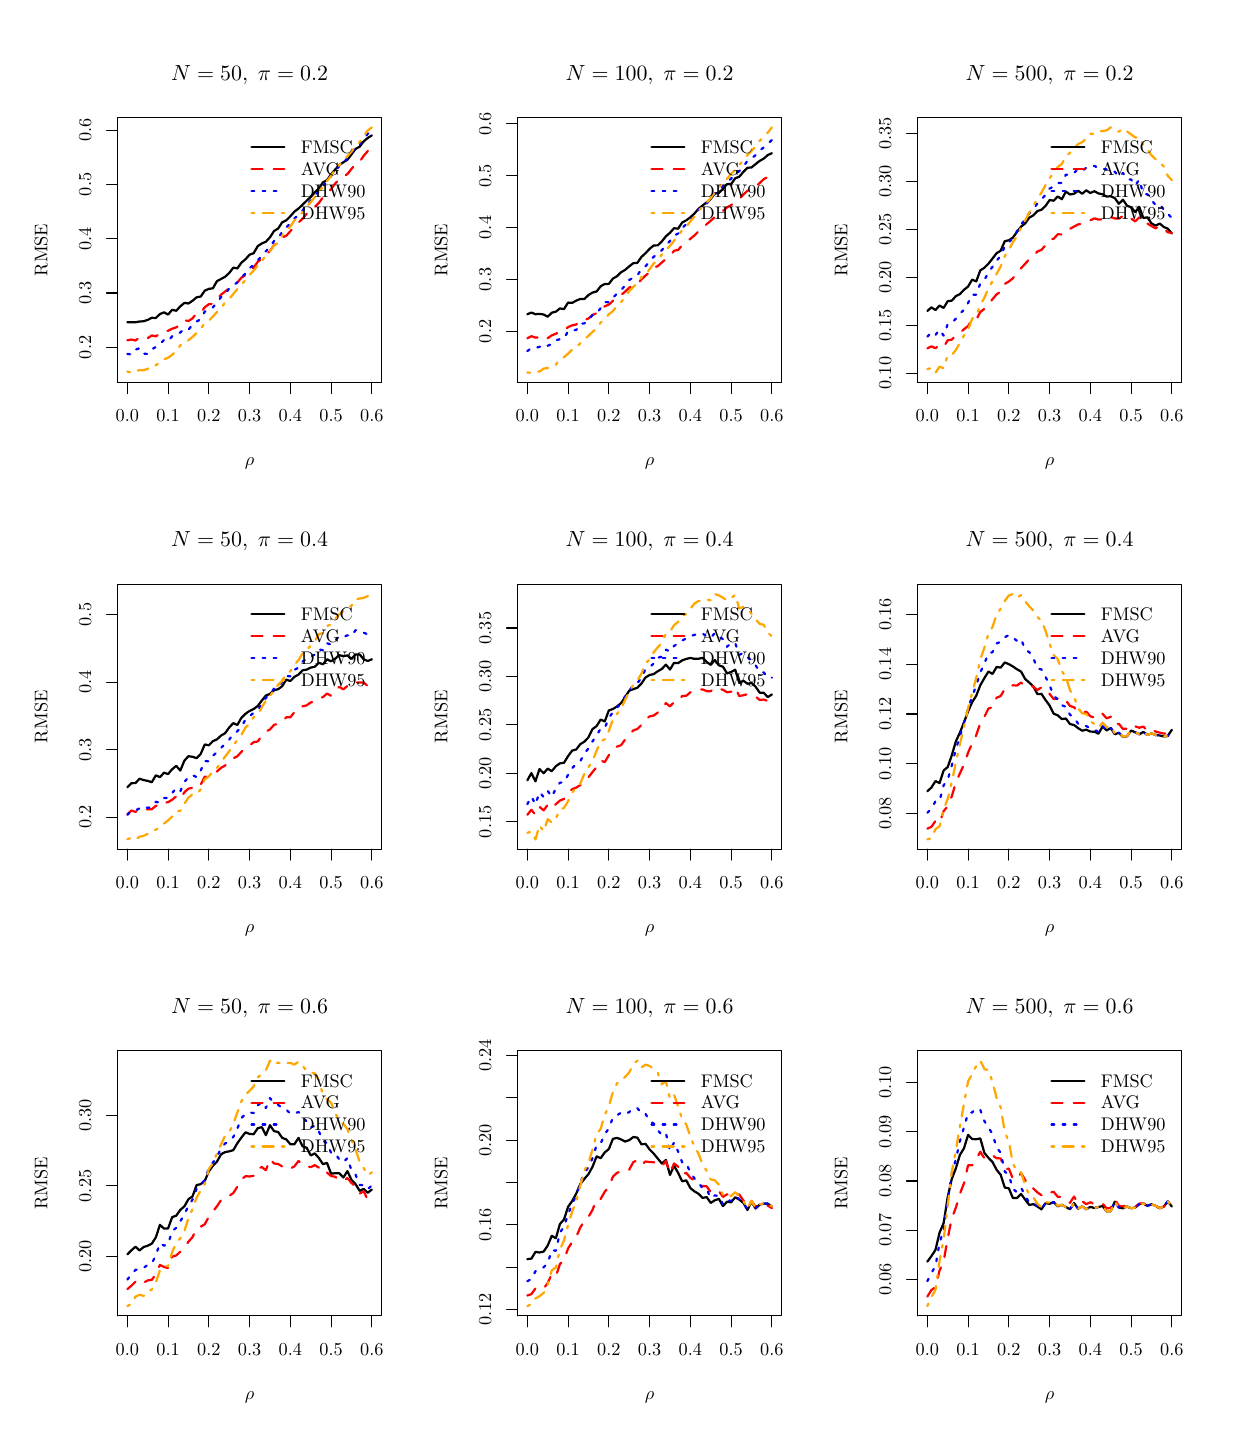
\begin{tikzpicture}[x=1pt,y=1pt]
\definecolor[named]{fillColor}{rgb}{1.00,1.00,1.00}
\path[use as bounding box,fill=fillColor,fill opacity=0.00] (0,0) rectangle (433.62,505.89);
\begin{scope}
\path[clip] ( 32.47,377.65) rectangle (127.91,473.42);
\definecolor[named]{drawColor}{rgb}{0.00,0.00,0.00}

\path[draw=drawColor,line width= 0.8pt,line join=round,line cap=round] ( 36.01,399.47) --
	( 37.48,399.47) --
	( 38.95,399.41) --
	( 40.42,399.71) --
	( 41.90,399.80) --
	( 43.37,400.28) --
	( 44.84,401.04) --
	( 46.32,400.99) --
	( 47.79,402.40) --
	( 49.26,403.03) --
	( 50.73,402.22) --
	( 52.21,403.94) --
	( 53.68,403.59) --
	( 55.15,405.19) --
	( 56.63,406.43) --
	( 58.10,406.22) --
	( 59.57,407.19) --
	( 61.04,408.46) --
	( 62.52,408.72) --
	( 63.99,410.85) --
	( 65.46,411.50) --
	( 66.93,411.71) --
	( 68.41,414.31) --
	( 69.88,415.08) --
	( 71.35,415.88) --
	( 72.83,417.24) --
	( 74.30,419.17) --
	( 75.77,418.89) --
	( 77.24,420.97) --
	( 78.72,422.22) --
	( 80.19,423.86) --
	( 81.66,424.39) --
	( 83.14,426.96) --
	( 84.61,427.92) --
	( 86.08,428.52) --
	( 87.55,430.12) --
	( 89.03,432.42) --
	( 90.50,433.29) --
	( 91.97,435.56) --
	( 93.44,436.26) --
	( 94.92,437.75) --
	( 96.39,439.42) --
	( 97.86,440.52) --
	( 99.34,441.93) --
	(100.81,443.36) --
	(102.28,444.71) --
	(103.75,446.39) --
	(105.23,447.80) --
	(106.70,450.00) --
	(108.17,450.78) --
	(109.65,452.94) --
	(111.12,454.63) --
	(112.59,456.24) --
	(114.06,457.24) --
	(115.54,458.16) --
	(117.01,460.09) --
	(118.48,462.06) --
	(119.95,462.87) --
	(121.43,464.80) --
	(122.90,466.05) --
	(124.37,466.95);
\end{scope}
\begin{scope}
\path[clip] (  0.00,  0.00) rectangle (433.62,505.89);
\definecolor[named]{drawColor}{rgb}{0.00,0.00,0.00}

\path[draw=drawColor,line width= 0.4pt,line join=round,line cap=round] ( 36.01,377.65) -- (124.37,377.65);

\path[draw=drawColor,line width= 0.4pt,line join=round,line cap=round] ( 36.01,377.65) -- ( 36.01,373.69);

\path[draw=drawColor,line width= 0.4pt,line join=round,line cap=round] ( 50.73,377.65) -- ( 50.73,373.69);

\path[draw=drawColor,line width= 0.4pt,line join=round,line cap=round] ( 65.46,377.65) -- ( 65.46,373.69);

\path[draw=drawColor,line width= 0.4pt,line join=round,line cap=round] ( 80.19,377.65) -- ( 80.19,373.69);

\path[draw=drawColor,line width= 0.4pt,line join=round,line cap=round] ( 94.92,377.65) -- ( 94.92,373.69);

\path[draw=drawColor,line width= 0.4pt,line join=round,line cap=round] (109.65,377.65) -- (109.65,373.69);

\path[draw=drawColor,line width= 0.4pt,line join=round,line cap=round] (124.37,377.65) -- (124.37,373.69);

\node[text=drawColor,anchor=base,inner sep=0pt, outer sep=0pt, scale=  0.66] at ( 36.01,363.40) {0.0};

\node[text=drawColor,anchor=base,inner sep=0pt, outer sep=0pt, scale=  0.66] at ( 50.73,363.40) {0.1};

\node[text=drawColor,anchor=base,inner sep=0pt, outer sep=0pt, scale=  0.66] at ( 65.46,363.40) {0.2};

\node[text=drawColor,anchor=base,inner sep=0pt, outer sep=0pt, scale=  0.66] at ( 80.19,363.40) {0.3};

\node[text=drawColor,anchor=base,inner sep=0pt, outer sep=0pt, scale=  0.66] at ( 94.92,363.40) {0.4};

\node[text=drawColor,anchor=base,inner sep=0pt, outer sep=0pt, scale=  0.66] at (109.65,363.40) {0.5};

\node[text=drawColor,anchor=base,inner sep=0pt, outer sep=0pt, scale=  0.66] at (124.37,363.40) {0.6};

\path[draw=drawColor,line width= 0.4pt,line join=round,line cap=round] ( 32.47,390.37) -- ( 32.47,468.88);

\path[draw=drawColor,line width= 0.4pt,line join=round,line cap=round] ( 32.47,390.37) -- ( 28.51,390.37);

\path[draw=drawColor,line width= 0.4pt,line join=round,line cap=round] ( 32.47,410.00) -- ( 28.51,410.00);

\path[draw=drawColor,line width= 0.4pt,line join=round,line cap=round] ( 32.47,429.62) -- ( 28.51,429.62);

\path[draw=drawColor,line width= 0.4pt,line join=round,line cap=round] ( 32.47,449.25) -- ( 28.51,449.25);

\path[draw=drawColor,line width= 0.4pt,line join=round,line cap=round] ( 32.47,468.88) -- ( 28.51,468.88);

\node[text=drawColor,rotate= 90.00,anchor=base,inner sep=0pt, outer sep=0pt, scale=  0.66] at ( 22.97,390.37) {0.2};

\node[text=drawColor,rotate= 90.00,anchor=base,inner sep=0pt, outer sep=0pt, scale=  0.66] at ( 22.97,410.00) {0.3};

\node[text=drawColor,rotate= 90.00,anchor=base,inner sep=0pt, outer sep=0pt, scale=  0.66] at ( 22.97,429.62) {0.4};

\node[text=drawColor,rotate= 90.00,anchor=base,inner sep=0pt, outer sep=0pt, scale=  0.66] at ( 22.97,449.25) {0.5};

\node[text=drawColor,rotate= 90.00,anchor=base,inner sep=0pt, outer sep=0pt, scale=  0.66] at ( 22.97,468.88) {0.6};

\path[draw=drawColor,line width= 0.4pt,line join=round,line cap=round] ( 32.47,377.65) --
	(127.91,377.65) --
	(127.91,473.42) --
	( 32.47,473.42) --
	( 32.47,377.65);
\end{scope}
\begin{scope}
\path[clip] (  0.00,337.26) rectangle (144.54,505.89);
\definecolor[named]{drawColor}{rgb}{0.00,0.00,0.00}

\node[text=drawColor,anchor=base,inner sep=0pt, outer sep=0pt, scale=  0.79] at ( 80.19,486.92) {\bfseries $N=50, \;\pi=0.2$};

\node[text=drawColor,anchor=base,inner sep=0pt, outer sep=0pt, scale=  0.66] at ( 80.19,347.56) {$\rho$};

\node[text=drawColor,rotate= 90.00,anchor=base,inner sep=0pt, outer sep=0pt, scale=  0.66] at (  7.13,425.53) {RMSE};
\end{scope}
\begin{scope}
\path[clip] ( 32.47,377.65) rectangle (127.91,473.42);
\definecolor[named]{drawColor}{rgb}{1.00,0.00,0.00}

\path[draw=drawColor,line width= 0.8pt,dash pattern=on 4pt off 4pt ,line join=round,line cap=round] ( 36.01,392.90) --
	( 37.48,393.20) --
	( 38.95,392.84) --
	( 40.42,393.97) --
	( 41.90,393.41) --
	( 43.37,393.70) --
	( 44.84,394.67) --
	( 46.32,394.33) --
	( 47.79,395.39) --
	( 49.26,396.30) --
	( 50.73,396.37) --
	( 52.21,397.11) --
	( 53.68,397.59) --
	( 55.15,398.61) --
	( 56.63,400.23) --
	( 58.10,399.85) --
	( 59.57,400.86) --
	( 61.04,402.76) --
	( 62.52,402.81) --
	( 63.99,404.86) --
	( 65.46,405.95) --
	( 66.93,406.12) --
	( 68.41,407.69) --
	( 69.88,409.39) --
	( 71.35,410.58) --
	( 72.83,411.67) --
	( 74.30,413.10) --
	( 75.77,413.80) --
	( 77.24,415.57) --
	( 78.72,416.45) --
	( 80.19,418.36) --
	( 81.66,419.20) --
	( 83.14,421.26) --
	( 84.61,422.48) --
	( 86.08,423.78) --
	( 87.55,425.22) --
	( 89.03,427.30) --
	( 90.50,428.21) --
	( 91.97,430.05) --
	( 93.44,430.69) --
	( 94.92,432.33) --
	( 96.39,434.26) --
	( 97.86,435.48) --
	( 99.34,436.84) --
	(100.81,438.65) --
	(102.28,439.82) --
	(103.75,441.08) --
	(105.23,442.56) --
	(106.70,444.59) --
	(108.17,446.14) --
	(109.65,447.51) --
	(111.12,449.60) --
	(112.59,451.04) --
	(114.06,451.97) --
	(115.54,453.00) --
	(117.01,454.84) --
	(118.48,456.64) --
	(119.95,457.37) --
	(121.43,459.60) --
	(122.90,461.30) --
	(124.37,461.90);
\definecolor[named]{drawColor}{rgb}{0.00,0.00,1.00}

\path[draw=drawColor,line width= 0.8pt,dash pattern=on 1pt off 3pt ,line join=round,line cap=round] ( 36.01,387.99) --
	( 37.48,387.83) --
	( 38.95,389.53) --
	( 40.42,390.06) --
	( 41.90,388.10) --
	( 43.37,387.97) --
	( 44.84,389.67) --
	( 46.32,390.50) --
	( 47.79,391.44) --
	( 49.26,393.07) --
	( 50.73,392.60) --
	( 52.21,394.37) --
	( 53.68,394.66) --
	( 55.15,395.77) --
	( 56.63,397.08) --
	( 58.10,396.80) --
	( 59.57,398.50) --
	( 61.04,399.68) --
	( 62.52,400.55) --
	( 63.99,403.32) --
	( 65.46,403.75) --
	( 66.93,404.82) --
	( 68.41,406.61) --
	( 69.88,408.51) --
	( 71.35,409.62) --
	( 72.83,411.69) --
	( 74.30,412.73) --
	( 75.77,413.85) --
	( 77.24,415.69) --
	( 78.72,417.06) --
	( 80.19,419.06) --
	( 81.66,420.06) --
	( 83.14,421.84) --
	( 84.61,423.39) --
	( 86.08,425.10) --
	( 87.55,426.68) --
	( 89.03,428.77) --
	( 90.50,429.68) --
	( 91.97,432.18) --
	( 93.44,433.64) --
	( 94.92,435.22) --
	( 96.39,436.96) --
	( 97.86,438.24) --
	( 99.34,439.80) --
	(100.81,441.80) --
	(102.28,443.40) --
	(103.75,445.27) --
	(105.23,446.72) --
	(106.70,448.79) --
	(108.17,450.27) --
	(109.65,452.29) --
	(111.12,454.38) --
	(112.59,455.75) --
	(114.06,457.10) --
	(115.54,458.70) --
	(117.01,460.46) --
	(118.48,462.67) --
	(119.95,463.56) --
	(121.43,465.64) --
	(122.90,467.55) --
	(124.37,468.42);
\definecolor[named]{drawColor}{rgb}{1.00,0.65,0.00}

\path[draw=drawColor,line width= 0.8pt,dash pattern=on 1pt off 3pt on 4pt off 3pt ,line join=round,line cap=round] ( 36.01,381.65) --
	( 37.48,381.20) --
	( 38.95,381.69) --
	( 40.42,382.15) --
	( 41.90,382.10) --
	( 43.37,382.56) --
	( 44.84,383.91) --
	( 46.32,383.88) --
	( 47.79,385.04) --
	( 49.26,386.04) --
	( 50.73,386.59) --
	( 52.21,387.72) --
	( 53.68,388.96) --
	( 55.15,391.10) --
	( 56.63,391.91) --
	( 58.10,392.95) --
	( 59.57,394.15) --
	( 61.04,395.56) --
	( 62.52,396.92) --
	( 63.99,399.31) --
	( 65.46,400.10) --
	( 66.93,401.49) --
	( 68.41,403.10) --
	( 69.88,404.49) --
	( 71.35,406.68) --
	( 72.83,407.84) --
	( 74.30,409.64) --
	( 75.77,411.46) --
	( 77.24,413.02) --
	( 78.72,414.74) --
	( 80.19,416.56) --
	( 81.66,418.11) --
	( 83.14,419.97) --
	( 84.61,421.48) --
	( 86.08,423.67) --
	( 87.55,425.15) --
	( 89.03,427.16) --
	( 90.50,428.18) --
	( 91.97,430.75) --
	( 93.44,432.41) --
	( 94.92,434.03) --
	( 96.39,436.22) --
	( 97.86,437.60) --
	( 99.34,439.08) --
	(100.81,441.24) --
	(102.28,442.83) --
	(103.75,444.80) --
	(105.23,446.18) --
	(106.70,448.66) --
	(108.17,450.46) --
	(109.65,452.40) --
	(111.12,454.59) --
	(112.59,456.17) --
	(114.06,457.68) --
	(115.54,459.45) --
	(117.01,461.12) --
	(118.48,463.24) --
	(119.95,464.57) --
	(121.43,466.80) --
	(122.90,468.74) --
	(124.37,469.87);
\definecolor[named]{drawColor}{rgb}{0.00,0.00,0.00}

\path[draw=drawColor,line width= 0.8pt,line join=round,line cap=round] ( 80.89,462.63) -- ( 92.77,462.63);
\definecolor[named]{drawColor}{rgb}{1.00,0.00,0.00}

\path[draw=drawColor,line width= 0.8pt,dash pattern=on 4pt off 4pt ,line join=round,line cap=round] ( 80.89,454.71) -- ( 92.77,454.71);
\definecolor[named]{drawColor}{rgb}{0.00,0.00,1.00}

\path[draw=drawColor,line width= 0.8pt,dash pattern=on 1pt off 3pt ,line join=round,line cap=round] ( 80.89,446.79) -- ( 92.77,446.79);
\definecolor[named]{drawColor}{rgb}{1.00,0.65,0.00}

\path[draw=drawColor,line width= 0.8pt,dash pattern=on 1pt off 3pt on 4pt off 3pt ,line join=round,line cap=round] ( 80.89,438.87) -- ( 92.77,438.87);
\definecolor[named]{drawColor}{rgb}{0.00,0.00,0.00}

\node[text=drawColor,anchor=base west,inner sep=0pt, outer sep=0pt, scale=  0.66] at ( 98.71,460.35) {FMSC};

\node[text=drawColor,anchor=base west,inner sep=0pt, outer sep=0pt, scale=  0.66] at ( 98.71,452.43) {AVG};

\node[text=drawColor,anchor=base west,inner sep=0pt, outer sep=0pt, scale=  0.66] at ( 98.71,444.51) {DHW90};

\node[text=drawColor,anchor=base west,inner sep=0pt, outer sep=0pt, scale=  0.66] at ( 98.71,436.59) {DHW95};
\end{scope}
\begin{scope}
\path[clip] (177.01,377.65) rectangle (272.45,473.42);
\definecolor[named]{drawColor}{rgb}{0.00,0.00,0.00}

\path[draw=drawColor,line width= 0.8pt,line join=round,line cap=round] (180.55,402.31) --
	(182.02,402.94) --
	(183.49,402.35) --
	(184.96,402.47) --
	(186.44,402.24) --
	(187.91,401.44) --
	(189.38,402.89) --
	(190.86,403.28) --
	(192.33,404.44) --
	(193.80,404.18) --
	(195.27,406.55) --
	(196.75,406.44) --
	(198.22,407.25) --
	(199.69,407.86) --
	(201.17,407.85) --
	(202.64,409.28) --
	(204.11,410.16) --
	(205.58,410.57) --
	(207.06,412.45) --
	(208.53,413.28) --
	(210.00,413.30) --
	(211.47,415.21) --
	(212.95,416.07) --
	(214.42,417.51) --
	(215.89,418.36) --
	(217.37,419.64) --
	(218.84,420.78) --
	(220.31,420.91) --
	(221.78,423.04) --
	(223.26,424.40) --
	(224.73,425.97) --
	(226.20,427.19) --
	(227.68,427.23) --
	(229.15,428.64) --
	(230.62,430.50) --
	(232.09,431.77) --
	(233.57,433.43) --
	(235.04,433.24) --
	(236.51,435.50) --
	(237.98,436.26) --
	(239.46,437.37) --
	(240.93,438.72) --
	(242.40,440.44) --
	(243.88,441.62) --
	(245.35,442.77) --
	(246.82,443.98) --
	(248.29,445.98) --
	(249.77,446.13) --
	(251.24,447.68) --
	(252.71,449.35) --
	(254.19,449.38) --
	(255.66,451.45) --
	(257.13,452.04) --
	(258.60,453.74) --
	(260.08,455.26) --
	(261.55,455.37) --
	(263.02,456.57) --
	(264.50,457.74) --
	(265.97,458.58) --
	(267.44,459.86) --
	(268.91,460.52);
\end{scope}
\begin{scope}
\path[clip] (  0.00,  0.00) rectangle (433.62,505.89);
\definecolor[named]{drawColor}{rgb}{0.00,0.00,0.00}

\path[draw=drawColor,line width= 0.4pt,line join=round,line cap=round] (180.55,377.65) -- (268.91,377.65);

\path[draw=drawColor,line width= 0.4pt,line join=round,line cap=round] (180.55,377.65) -- (180.55,373.69);

\path[draw=drawColor,line width= 0.4pt,line join=round,line cap=round] (195.27,377.65) -- (195.27,373.69);

\path[draw=drawColor,line width= 0.4pt,line join=round,line cap=round] (210.00,377.65) -- (210.00,373.69);

\path[draw=drawColor,line width= 0.4pt,line join=round,line cap=round] (224.73,377.65) -- (224.73,373.69);

\path[draw=drawColor,line width= 0.4pt,line join=round,line cap=round] (239.46,377.65) -- (239.46,373.69);

\path[draw=drawColor,line width= 0.4pt,line join=round,line cap=round] (254.19,377.65) -- (254.19,373.69);

\path[draw=drawColor,line width= 0.4pt,line join=round,line cap=round] (268.91,377.65) -- (268.91,373.69);

\node[text=drawColor,anchor=base,inner sep=0pt, outer sep=0pt, scale=  0.66] at (180.55,363.40) {0.0};

\node[text=drawColor,anchor=base,inner sep=0pt, outer sep=0pt, scale=  0.66] at (195.27,363.40) {0.1};

\node[text=drawColor,anchor=base,inner sep=0pt, outer sep=0pt, scale=  0.66] at (210.00,363.40) {0.2};

\node[text=drawColor,anchor=base,inner sep=0pt, outer sep=0pt, scale=  0.66] at (224.73,363.40) {0.3};

\node[text=drawColor,anchor=base,inner sep=0pt, outer sep=0pt, scale=  0.66] at (239.46,363.40) {0.4};

\node[text=drawColor,anchor=base,inner sep=0pt, outer sep=0pt, scale=  0.66] at (254.19,363.40) {0.5};

\node[text=drawColor,anchor=base,inner sep=0pt, outer sep=0pt, scale=  0.66] at (268.91,363.40) {0.6};

\path[draw=drawColor,line width= 0.4pt,line join=round,line cap=round] (177.01,396.12) -- (177.01,471.23);

\path[draw=drawColor,line width= 0.4pt,line join=round,line cap=round] (177.01,396.12) -- (173.05,396.12);

\path[draw=drawColor,line width= 0.4pt,line join=round,line cap=round] (177.01,414.90) -- (173.05,414.90);

\path[draw=drawColor,line width= 0.4pt,line join=round,line cap=round] (177.01,433.68) -- (173.05,433.68);

\path[draw=drawColor,line width= 0.4pt,line join=round,line cap=round] (177.01,452.45) -- (173.05,452.45);

\path[draw=drawColor,line width= 0.4pt,line join=round,line cap=round] (177.01,471.23) -- (173.05,471.23);

\node[text=drawColor,rotate= 90.00,anchor=base,inner sep=0pt, outer sep=0pt, scale=  0.66] at (167.51,396.12) {0.2};

\node[text=drawColor,rotate= 90.00,anchor=base,inner sep=0pt, outer sep=0pt, scale=  0.66] at (167.51,414.90) {0.3};

\node[text=drawColor,rotate= 90.00,anchor=base,inner sep=0pt, outer sep=0pt, scale=  0.66] at (167.51,433.68) {0.4};

\node[text=drawColor,rotate= 90.00,anchor=base,inner sep=0pt, outer sep=0pt, scale=  0.66] at (167.51,452.45) {0.5};

\node[text=drawColor,rotate= 90.00,anchor=base,inner sep=0pt, outer sep=0pt, scale=  0.66] at (167.51,471.23) {0.6};

\path[draw=drawColor,line width= 0.4pt,line join=round,line cap=round] (177.01,377.65) --
	(272.45,377.65) --
	(272.45,473.42) --
	(177.01,473.42) --
	(177.01,377.65);
\end{scope}
\begin{scope}
\path[clip] (144.54,337.26) rectangle (289.08,505.89);
\definecolor[named]{drawColor}{rgb}{0.00,0.00,0.00}

\node[text=drawColor,anchor=base,inner sep=0pt, outer sep=0pt, scale=  0.79] at (224.73,486.92) {\bfseries $N=100, \;\pi=0.2$};

\node[text=drawColor,anchor=base,inner sep=0pt, outer sep=0pt, scale=  0.66] at (224.73,347.56) {$\rho$};

\node[text=drawColor,rotate= 90.00,anchor=base,inner sep=0pt, outer sep=0pt, scale=  0.66] at (151.67,425.53) {RMSE};
\end{scope}
\begin{scope}
\path[clip] (177.01,377.65) rectangle (272.45,473.42);
\definecolor[named]{drawColor}{rgb}{1.00,0.00,0.00}

\path[draw=drawColor,line width= 0.8pt,dash pattern=on 4pt off 4pt ,line join=round,line cap=round] (180.55,393.63) --
	(182.02,394.41) --
	(183.49,393.87) --
	(184.96,394.07) --
	(186.44,394.69) --
	(187.91,393.69) --
	(189.38,394.70) --
	(190.86,395.28) --
	(192.33,396.19) --
	(193.80,396.54) --
	(195.27,397.69) --
	(196.75,398.31) --
	(198.22,398.63) --
	(199.69,400.00) --
	(201.17,400.20) --
	(202.64,400.81) --
	(204.11,402.04) --
	(205.58,402.75) --
	(207.06,404.44) --
	(208.53,405.18) --
	(210.00,405.84) --
	(211.47,407.16) --
	(212.95,408.50) --
	(214.42,409.23) --
	(215.89,410.50) --
	(217.37,411.95) --
	(218.84,412.87) --
	(220.31,413.22) --
	(221.78,414.92) --
	(223.26,416.32) --
	(224.73,417.47) --
	(226.20,419.24) --
	(227.68,419.70) --
	(229.15,421.03) --
	(230.62,422.30) --
	(232.09,423.30) --
	(233.57,425.28) --
	(235.04,425.53) --
	(236.51,427.38) --
	(237.98,428.53) --
	(239.46,429.59) --
	(240.93,430.82) --
	(242.40,432.27) --
	(243.88,433.32) --
	(245.35,434.89) --
	(246.82,436.12) --
	(248.29,437.45) --
	(249.77,438.59) --
	(251.24,439.65) --
	(252.71,440.93) --
	(254.19,441.75) --
	(255.66,443.04) --
	(257.13,444.01) --
	(258.60,445.54) --
	(260.08,446.97) --
	(261.55,447.28) --
	(263.02,448.38) --
	(264.50,449.74) --
	(265.97,451.14) --
	(267.44,451.94) --
	(268.91,453.28);
\definecolor[named]{drawColor}{rgb}{0.00,0.00,1.00}

\path[draw=drawColor,line width= 0.8pt,dash pattern=on 1pt off 3pt ,line join=round,line cap=round] (180.55,389.02) --
	(182.02,390.11) --
	(183.49,390.20) --
	(184.96,390.54) --
	(186.44,391.36) --
	(187.91,390.96) --
	(189.38,391.58) --
	(190.86,392.92) --
	(192.33,393.32) --
	(193.80,393.59) --
	(195.27,396.19) --
	(196.75,396.47) --
	(198.22,396.65) --
	(199.69,398.85) --
	(201.17,399.04) --
	(202.64,400.10) --
	(204.11,402.13) --
	(205.58,402.58) --
	(207.06,404.56) --
	(208.53,406.72) --
	(210.00,406.69) --
	(211.47,408.25) --
	(212.95,409.80) --
	(214.42,410.96) --
	(215.89,412.83) --
	(217.37,414.70) --
	(218.84,415.58) --
	(220.31,416.33) --
	(221.78,418.73) --
	(223.26,419.68) --
	(224.73,421.37) --
	(226.20,423.09) --
	(227.68,424.07) --
	(229.15,425.47) --
	(230.62,427.28) --
	(232.09,428.78) --
	(233.57,430.79) --
	(235.04,431.50) --
	(236.51,433.54) --
	(237.98,434.84) --
	(239.46,436.17) --
	(240.93,437.95) --
	(242.40,440.14) --
	(243.88,441.26) --
	(245.35,442.37) --
	(246.82,444.09) --
	(248.29,445.89) --
	(249.77,447.31) --
	(251.24,448.68) --
	(252.71,450.07) --
	(254.19,451.33) --
	(255.66,452.91) --
	(257.13,454.05) --
	(258.60,455.67) --
	(260.08,457.75) --
	(261.55,458.56) --
	(263.02,459.84) --
	(264.50,461.53) --
	(265.97,462.59) --
	(267.44,463.93) --
	(268.91,465.31);
\definecolor[named]{drawColor}{rgb}{1.00,0.65,0.00}

\path[draw=drawColor,line width= 0.8pt,dash pattern=on 1pt off 3pt on 4pt off 3pt ,line join=round,line cap=round] (180.55,381.26) --
	(182.02,381.20) --
	(183.49,381.72) --
	(184.96,381.59) --
	(186.44,382.70) --
	(187.91,382.87) --
	(189.38,383.27) --
	(190.86,384.13) --
	(192.33,386.13) --
	(193.80,386.83) --
	(195.27,388.07) --
	(196.75,389.59) --
	(198.22,390.27) --
	(199.69,391.88) --
	(201.17,393.21) --
	(202.64,394.54) --
	(204.11,395.96) --
	(205.58,397.23) --
	(207.06,399.31) --
	(208.53,400.59) --
	(210.00,402.31) --
	(211.47,403.46) --
	(212.95,405.32) --
	(214.42,406.68) --
	(215.89,408.60) --
	(217.37,410.69) --
	(218.84,412.22) --
	(220.31,413.48) --
	(221.78,415.70) --
	(223.26,416.54) --
	(224.73,418.61) --
	(226.20,420.63) --
	(227.68,422.01) --
	(229.15,423.87) --
	(230.62,425.48) --
	(232.09,427.04) --
	(233.57,428.86) --
	(235.04,430.73) --
	(236.51,432.72) --
	(237.98,433.92) --
	(239.46,435.87) --
	(240.93,437.61) --
	(242.40,439.65) --
	(243.88,441.18) --
	(245.35,442.70) --
	(246.82,444.33) --
	(248.29,446.37) --
	(249.77,448.22) --
	(251.24,449.65) --
	(252.71,451.22) --
	(254.19,453.10) --
	(255.66,454.57) --
	(257.13,456.19) --
	(258.60,458.05) --
	(260.08,459.82) --
	(261.55,461.36) --
	(263.02,462.93) --
	(264.50,465.01) --
	(265.97,466.30) --
	(267.44,467.97) --
	(268.91,469.87);
\definecolor[named]{drawColor}{rgb}{0.00,0.00,0.00}

\path[draw=drawColor,line width= 0.8pt,line join=round,line cap=round] (225.43,462.63) -- (237.31,462.63);
\definecolor[named]{drawColor}{rgb}{1.00,0.00,0.00}

\path[draw=drawColor,line width= 0.8pt,dash pattern=on 4pt off 4pt ,line join=round,line cap=round] (225.43,454.71) -- (237.31,454.71);
\definecolor[named]{drawColor}{rgb}{0.00,0.00,1.00}

\path[draw=drawColor,line width= 0.8pt,dash pattern=on 1pt off 3pt ,line join=round,line cap=round] (225.43,446.79) -- (237.31,446.79);
\definecolor[named]{drawColor}{rgb}{1.00,0.65,0.00}

\path[draw=drawColor,line width= 0.8pt,dash pattern=on 1pt off 3pt on 4pt off 3pt ,line join=round,line cap=round] (225.43,438.87) -- (237.31,438.87);
\definecolor[named]{drawColor}{rgb}{0.00,0.00,0.00}

\node[text=drawColor,anchor=base west,inner sep=0pt, outer sep=0pt, scale=  0.66] at (243.25,460.35) {FMSC};

\node[text=drawColor,anchor=base west,inner sep=0pt, outer sep=0pt, scale=  0.66] at (243.25,452.43) {AVG};

\node[text=drawColor,anchor=base west,inner sep=0pt, outer sep=0pt, scale=  0.66] at (243.25,444.51) {DHW90};

\node[text=drawColor,anchor=base west,inner sep=0pt, outer sep=0pt, scale=  0.66] at (243.25,436.59) {DHW95};
\end{scope}
\begin{scope}
\path[clip] (321.55,377.65) rectangle (416.99,473.42);
\definecolor[named]{drawColor}{rgb}{0.00,0.00,0.00}

\path[draw=drawColor,line width= 0.8pt,line join=round,line cap=round] (325.09,403.51) --
	(326.56,404.81) --
	(328.03,403.86) --
	(329.50,405.48) --
	(330.98,404.61) --
	(332.45,407.06) --
	(333.92,407.25) --
	(335.40,408.88) --
	(336.87,409.63) --
	(338.34,411.18) --
	(339.81,412.34) --
	(341.29,414.85) --
	(342.76,414.20) --
	(344.23,418.20) --
	(345.71,419.12) --
	(347.18,420.62) --
	(348.65,422.48) --
	(350.12,424.39) --
	(351.60,425.29) --
	(353.07,428.74) --
	(354.54,429.06) --
	(356.01,430.03) --
	(357.49,432.10) --
	(358.96,433.99) --
	(360.43,435.15) --
	(361.91,437.24) --
	(363.38,438.05) --
	(364.85,439.62) --
	(366.32,440.09) --
	(367.80,441.47) --
	(369.27,443.60) --
	(370.74,443.36) --
	(372.22,444.89) --
	(373.69,443.89) --
	(375.16,446.65) --
	(376.63,445.61) --
	(378.11,445.87) --
	(379.58,446.95) --
	(381.05,445.87) --
	(382.52,447.12) --
	(384.00,446.14) --
	(385.47,446.79) --
	(386.94,445.97) --
	(388.42,445.69) --
	(389.89,444.85) --
	(391.36,444.99) --
	(392.83,444.29) --
	(394.31,442.25) --
	(395.78,443.71) --
	(397.25,441.55) --
	(398.73,441.01) --
	(400.20,439.23) --
	(401.67,441.12) --
	(403.14,437.11) --
	(404.62,437.36) --
	(406.09,435.16) --
	(407.56,434.34) --
	(409.04,435.11) --
	(410.51,433.89) --
	(411.98,433.24) --
	(413.45,431.52);
\end{scope}
\begin{scope}
\path[clip] (  0.00,  0.00) rectangle (433.62,505.89);
\definecolor[named]{drawColor}{rgb}{0.00,0.00,0.00}

\path[draw=drawColor,line width= 0.4pt,line join=round,line cap=round] (325.09,377.65) -- (413.45,377.65);

\path[draw=drawColor,line width= 0.4pt,line join=round,line cap=round] (325.09,377.65) -- (325.09,373.69);

\path[draw=drawColor,line width= 0.4pt,line join=round,line cap=round] (339.81,377.65) -- (339.81,373.69);

\path[draw=drawColor,line width= 0.4pt,line join=round,line cap=round] (354.54,377.65) -- (354.54,373.69);

\path[draw=drawColor,line width= 0.4pt,line join=round,line cap=round] (369.27,377.65) -- (369.27,373.69);

\path[draw=drawColor,line width= 0.4pt,line join=round,line cap=round] (384.00,377.65) -- (384.00,373.69);

\path[draw=drawColor,line width= 0.4pt,line join=round,line cap=round] (398.73,377.65) -- (398.73,373.69);

\path[draw=drawColor,line width= 0.4pt,line join=round,line cap=round] (413.45,377.65) -- (413.45,373.69);

\node[text=drawColor,anchor=base,inner sep=0pt, outer sep=0pt, scale=  0.66] at (325.09,363.40) {0.0};

\node[text=drawColor,anchor=base,inner sep=0pt, outer sep=0pt, scale=  0.66] at (339.81,363.40) {0.1};

\node[text=drawColor,anchor=base,inner sep=0pt, outer sep=0pt, scale=  0.66] at (354.54,363.40) {0.2};

\node[text=drawColor,anchor=base,inner sep=0pt, outer sep=0pt, scale=  0.66] at (369.27,363.40) {0.3};

\node[text=drawColor,anchor=base,inner sep=0pt, outer sep=0pt, scale=  0.66] at (384.00,363.40) {0.4};

\node[text=drawColor,anchor=base,inner sep=0pt, outer sep=0pt, scale=  0.66] at (398.73,363.40) {0.5};

\node[text=drawColor,anchor=base,inner sep=0pt, outer sep=0pt, scale=  0.66] at (413.45,363.40) {0.6};

\path[draw=drawColor,line width= 0.4pt,line join=round,line cap=round] (321.55,381.08) -- (321.55,467.59);

\path[draw=drawColor,line width= 0.4pt,line join=round,line cap=round] (321.55,381.08) -- (317.59,381.08);

\path[draw=drawColor,line width= 0.4pt,line join=round,line cap=round] (321.55,398.38) -- (317.59,398.38);

\path[draw=drawColor,line width= 0.4pt,line join=round,line cap=round] (321.55,415.68) -- (317.59,415.68);

\path[draw=drawColor,line width= 0.4pt,line join=round,line cap=round] (321.55,432.99) -- (317.59,432.99);

\path[draw=drawColor,line width= 0.4pt,line join=round,line cap=round] (321.55,450.29) -- (317.59,450.29);

\path[draw=drawColor,line width= 0.4pt,line join=round,line cap=round] (321.55,467.59) -- (317.59,467.59);

\node[text=drawColor,rotate= 90.00,anchor=base,inner sep=0pt, outer sep=0pt, scale=  0.66] at (312.05,381.08) {0.10};

\node[text=drawColor,rotate= 90.00,anchor=base,inner sep=0pt, outer sep=0pt, scale=  0.66] at (312.05,398.38) {0.15};

\node[text=drawColor,rotate= 90.00,anchor=base,inner sep=0pt, outer sep=0pt, scale=  0.66] at (312.05,415.68) {0.20};

\node[text=drawColor,rotate= 90.00,anchor=base,inner sep=0pt, outer sep=0pt, scale=  0.66] at (312.05,432.99) {0.25};

\node[text=drawColor,rotate= 90.00,anchor=base,inner sep=0pt, outer sep=0pt, scale=  0.66] at (312.05,450.29) {0.30};

\node[text=drawColor,rotate= 90.00,anchor=base,inner sep=0pt, outer sep=0pt, scale=  0.66] at (312.05,467.59) {0.35};

\path[draw=drawColor,line width= 0.4pt,line join=round,line cap=round] (321.55,377.65) --
	(416.99,377.65) --
	(416.99,473.42) --
	(321.55,473.42) --
	(321.55,377.65);
\end{scope}
\begin{scope}
\path[clip] (289.08,337.26) rectangle (433.62,505.89);
\definecolor[named]{drawColor}{rgb}{0.00,0.00,0.00}

\node[text=drawColor,anchor=base,inner sep=0pt, outer sep=0pt, scale=  0.79] at (369.27,486.92) {\bfseries $N=500, \;\pi=0.2$};

\node[text=drawColor,anchor=base,inner sep=0pt, outer sep=0pt, scale=  0.66] at (369.27,347.56) {$\rho$};

\node[text=drawColor,rotate= 90.00,anchor=base,inner sep=0pt, outer sep=0pt, scale=  0.66] at (296.21,425.53) {RMSE};
\end{scope}
\begin{scope}
\path[clip] (321.55,377.65) rectangle (416.99,473.42);
\definecolor[named]{drawColor}{rgb}{1.00,0.00,0.00}

\path[draw=drawColor,line width= 0.8pt,dash pattern=on 4pt off 4pt ,line join=round,line cap=round] (325.09,389.97) --
	(326.56,390.74) --
	(328.03,390.05) --
	(329.50,391.19) --
	(330.98,390.54) --
	(332.45,392.90) --
	(333.92,393.16) --
	(335.40,394.67) --
	(336.87,395.59) --
	(338.34,396.91) --
	(339.81,398.10) --
	(341.29,400.49) --
	(342.76,400.32) --
	(344.23,403.16) --
	(345.71,404.27) --
	(347.18,406.03) --
	(348.65,407.78) --
	(350.12,409.54) --
	(351.60,410.47) --
	(353.07,413.29) --
	(354.54,414.16) --
	(356.01,415.32) --
	(357.49,417.41) --
	(358.96,418.98) --
	(360.43,420.55) --
	(361.91,422.26) --
	(363.38,423.32) --
	(364.85,424.99) --
	(366.32,425.60) --
	(367.80,427.28) --
	(369.27,429.40) --
	(370.74,429.60) --
	(372.22,431.21) --
	(373.69,431.18) --
	(375.16,432.74) --
	(376.63,433.19) --
	(378.11,434.01) --
	(379.58,434.80) --
	(381.05,435.03) --
	(382.52,435.71) --
	(384.00,436.27) --
	(385.47,436.97) --
	(386.94,436.54) --
	(388.42,436.56) --
	(389.89,436.78) --
	(391.36,437.47) --
	(392.83,436.94) --
	(394.31,436.91) --
	(395.78,437.84) --
	(397.25,436.61) --
	(398.73,436.89) --
	(400.20,435.90) --
	(401.67,437.30) --
	(403.14,434.88) --
	(404.62,435.11) --
	(406.09,434.20) --
	(407.56,433.39) --
	(409.04,434.20) --
	(410.51,433.29) --
	(411.98,431.97) --
	(413.45,431.68);
\definecolor[named]{drawColor}{rgb}{0.00,0.00,1.00}

\path[draw=drawColor,line width= 0.8pt,dash pattern=on 1pt off 3pt ,line join=round,line cap=round] (325.09,394.22) --
	(326.56,395.79) --
	(328.03,394.84) --
	(329.50,396.74) --
	(330.98,394.62) --
	(332.45,398.76) --
	(333.92,399.16) --
	(335.40,400.75) --
	(336.87,402.58) --
	(338.34,403.92) --
	(339.81,406.42) --
	(341.29,409.41) --
	(342.76,409.39) --
	(344.23,413.48) --
	(345.71,414.75) --
	(347.18,417.39) --
	(348.65,419.51) --
	(350.12,421.67) --
	(351.60,423.45) --
	(353.07,426.82) --
	(354.54,428.31) --
	(356.01,429.95) --
	(357.49,432.30) --
	(358.96,434.81) --
	(360.43,436.46) --
	(361.91,438.81) --
	(363.38,440.24) --
	(364.85,442.36) --
	(366.32,443.87) --
	(367.80,445.44) --
	(369.27,447.74) --
	(370.74,448.50) --
	(372.22,449.78) --
	(373.69,449.80) --
	(375.16,452.79) --
	(376.63,452.56) --
	(378.11,453.43) --
	(379.58,454.73) --
	(381.05,454.12) --
	(382.52,455.24) --
	(384.00,455.25) --
	(385.47,455.97) --
	(386.94,455.02) --
	(388.42,454.89) --
	(389.89,454.66) --
	(391.36,454.74) --
	(392.83,453.77) --
	(394.31,452.06) --
	(395.78,453.37) --
	(397.25,451.20) --
	(398.73,451.00) --
	(400.20,448.88) --
	(401.67,450.95) --
	(403.14,445.80) --
	(404.62,445.70) --
	(406.09,443.53) --
	(407.56,441.84) --
	(409.04,442.10) --
	(410.51,440.10) --
	(411.98,438.72) --
	(413.45,437.02);
\definecolor[named]{drawColor}{rgb}{1.00,0.65,0.00}

\path[draw=drawColor,line width= 0.8pt,dash pattern=on 1pt off 3pt on 4pt off 3pt ,line join=round,line cap=round] (325.09,382.47) --
	(326.56,382.95) --
	(328.03,381.20) --
	(329.50,383.42) --
	(330.98,382.79) --
	(332.45,387.50) --
	(333.92,387.66) --
	(335.40,389.41) --
	(336.87,392.06) --
	(338.34,394.69) --
	(339.81,396.84) --
	(341.29,400.68) --
	(342.76,401.78) --
	(344.23,405.67) --
	(345.71,408.28) --
	(347.18,411.79) --
	(348.65,414.27) --
	(350.12,416.93) --
	(351.60,419.62) --
	(353.07,423.30) --
	(354.54,425.55) --
	(356.01,428.39) --
	(357.49,430.49) --
	(358.96,433.62) --
	(360.43,436.19) --
	(361.91,439.08) --
	(363.38,441.65) --
	(364.85,443.90) --
	(366.32,446.28) --
	(367.80,448.99) --
	(369.27,451.53) --
	(370.74,453.40) --
	(372.22,455.59) --
	(373.69,456.62) --
	(375.16,459.41) --
	(376.63,460.66) --
	(378.11,462.19) --
	(379.58,463.84) --
	(381.05,464.51) --
	(382.52,465.83) --
	(384.00,467.52) --
	(385.47,467.62) --
	(386.94,468.43) --
	(388.42,468.50) --
	(389.89,468.80) --
	(391.36,469.87) --
	(392.83,468.98) --
	(394.31,468.29) --
	(395.78,469.43) --
	(397.25,468.41) --
	(398.73,467.29) --
	(400.20,466.22) --
	(401.67,466.20) --
	(403.14,463.61) --
	(404.62,461.86) --
	(406.09,459.76) --
	(407.56,458.37) --
	(409.04,457.42) --
	(410.51,455.71) --
	(411.98,452.35) --
	(413.45,450.81);
\definecolor[named]{drawColor}{rgb}{0.00,0.00,0.00}

\path[draw=drawColor,line width= 0.8pt,line join=round,line cap=round] (369.97,462.63) -- (381.85,462.63);
\definecolor[named]{drawColor}{rgb}{1.00,0.00,0.00}

\path[draw=drawColor,line width= 0.8pt,dash pattern=on 4pt off 4pt ,line join=round,line cap=round] (369.97,454.71) -- (381.85,454.71);
\definecolor[named]{drawColor}{rgb}{0.00,0.00,1.00}

\path[draw=drawColor,line width= 0.8pt,dash pattern=on 1pt off 3pt ,line join=round,line cap=round] (369.97,446.79) -- (381.85,446.79);
\definecolor[named]{drawColor}{rgb}{1.00,0.65,0.00}

\path[draw=drawColor,line width= 0.8pt,dash pattern=on 1pt off 3pt on 4pt off 3pt ,line join=round,line cap=round] (369.97,438.87) -- (381.85,438.87);
\definecolor[named]{drawColor}{rgb}{0.00,0.00,0.00}

\node[text=drawColor,anchor=base west,inner sep=0pt, outer sep=0pt, scale=  0.66] at (387.79,460.35) {FMSC};

\node[text=drawColor,anchor=base west,inner sep=0pt, outer sep=0pt, scale=  0.66] at (387.79,452.43) {AVG};

\node[text=drawColor,anchor=base west,inner sep=0pt, outer sep=0pt, scale=  0.66] at (387.79,444.51) {DHW90};

\node[text=drawColor,anchor=base west,inner sep=0pt, outer sep=0pt, scale=  0.66] at (387.79,436.59) {DHW95};
\end{scope}
\begin{scope}
\path[clip] ( 32.47,209.02) rectangle (127.91,304.79);
\definecolor[named]{drawColor}{rgb}{0.00,0.00,0.00}

\path[draw=drawColor,line width= 0.8pt,line join=round,line cap=round] ( 36.01,231.39) --
	( 37.48,232.89) --
	( 38.95,232.91) --
	( 40.42,234.50) --
	( 41.90,234.01) --
	( 43.37,233.72) --
	( 44.84,233.22) --
	( 46.32,235.72) --
	( 47.79,235.06) --
	( 49.26,236.66) --
	( 50.73,236.19) --
	( 52.21,237.93) --
	( 53.68,239.14) --
	( 55.15,237.45) --
	( 56.63,241.02) --
	( 58.10,242.64) --
	( 59.57,242.42) --
	( 61.04,241.92) --
	( 62.52,243.44) --
	( 63.99,246.87) --
	( 65.46,246.56) --
	( 66.93,248.07) --
	( 68.41,248.73) --
	( 69.88,250.09) --
	( 71.35,250.94) --
	( 72.83,253.02) --
	( 74.30,254.58) --
	( 75.77,253.92) --
	( 77.24,256.52) --
	( 78.72,257.97) --
	( 80.19,258.98) --
	( 81.66,259.68) --
	( 83.14,260.77) --
	( 84.61,262.74) --
	( 86.08,264.57) --
	( 87.55,265.13) --
	( 89.03,266.46) --
	( 90.50,266.85) --
	( 91.97,267.92) --
	( 93.44,270.30) --
	( 94.92,269.78) --
	( 96.39,271.31) --
	( 97.86,272.11) --
	( 99.34,273.67) --
	(100.81,273.92) --
	(102.28,274.65) --
	(103.75,274.96) --
	(105.23,276.39) --
	(106.70,275.83) --
	(108.17,277.62) --
	(109.65,276.93) --
	(111.12,277.88) --
	(112.59,279.14) --
	(114.06,278.79) --
	(115.54,279.04) --
	(117.01,277.80) --
	(118.48,279.41) --
	(119.95,279.41) --
	(121.43,277.63) --
	(122.90,277.05) --
	(124.37,277.66);
\end{scope}
\begin{scope}
\path[clip] (  0.00,  0.00) rectangle (433.62,505.89);
\definecolor[named]{drawColor}{rgb}{0.00,0.00,0.00}

\path[draw=drawColor,line width= 0.4pt,line join=round,line cap=round] ( 36.01,209.02) -- (124.37,209.02);

\path[draw=drawColor,line width= 0.4pt,line join=round,line cap=round] ( 36.01,209.02) -- ( 36.01,205.06);

\path[draw=drawColor,line width= 0.4pt,line join=round,line cap=round] ( 50.73,209.02) -- ( 50.73,205.06);

\path[draw=drawColor,line width= 0.4pt,line join=round,line cap=round] ( 65.46,209.02) -- ( 65.46,205.06);

\path[draw=drawColor,line width= 0.4pt,line join=round,line cap=round] ( 80.19,209.02) -- ( 80.19,205.06);

\path[draw=drawColor,line width= 0.4pt,line join=round,line cap=round] ( 94.92,209.02) -- ( 94.92,205.06);

\path[draw=drawColor,line width= 0.4pt,line join=round,line cap=round] (109.65,209.02) -- (109.65,205.06);

\path[draw=drawColor,line width= 0.4pt,line join=round,line cap=round] (124.37,209.02) -- (124.37,205.06);

\node[text=drawColor,anchor=base,inner sep=0pt, outer sep=0pt, scale=  0.66] at ( 36.01,194.77) {0.0};

\node[text=drawColor,anchor=base,inner sep=0pt, outer sep=0pt, scale=  0.66] at ( 50.73,194.77) {0.1};

\node[text=drawColor,anchor=base,inner sep=0pt, outer sep=0pt, scale=  0.66] at ( 65.46,194.77) {0.2};

\node[text=drawColor,anchor=base,inner sep=0pt, outer sep=0pt, scale=  0.66] at ( 80.19,194.77) {0.3};

\node[text=drawColor,anchor=base,inner sep=0pt, outer sep=0pt, scale=  0.66] at ( 94.92,194.77) {0.4};

\node[text=drawColor,anchor=base,inner sep=0pt, outer sep=0pt, scale=  0.66] at (109.65,194.77) {0.5};

\node[text=drawColor,anchor=base,inner sep=0pt, outer sep=0pt, scale=  0.66] at (124.37,194.77) {0.6};

\path[draw=drawColor,line width= 0.4pt,line join=round,line cap=round] ( 32.47,220.56) -- ( 32.47,293.85);

\path[draw=drawColor,line width= 0.4pt,line join=round,line cap=round] ( 32.47,220.56) -- ( 28.51,220.56);

\path[draw=drawColor,line width= 0.4pt,line join=round,line cap=round] ( 32.47,244.99) -- ( 28.51,244.99);

\path[draw=drawColor,line width= 0.4pt,line join=round,line cap=round] ( 32.47,269.42) -- ( 28.51,269.42);

\path[draw=drawColor,line width= 0.4pt,line join=round,line cap=round] ( 32.47,293.85) -- ( 28.51,293.85);

\node[text=drawColor,rotate= 90.00,anchor=base,inner sep=0pt, outer sep=0pt, scale=  0.66] at ( 22.97,220.56) {0.2};

\node[text=drawColor,rotate= 90.00,anchor=base,inner sep=0pt, outer sep=0pt, scale=  0.66] at ( 22.97,244.99) {0.3};

\node[text=drawColor,rotate= 90.00,anchor=base,inner sep=0pt, outer sep=0pt, scale=  0.66] at ( 22.97,269.42) {0.4};

\node[text=drawColor,rotate= 90.00,anchor=base,inner sep=0pt, outer sep=0pt, scale=  0.66] at ( 22.97,293.85) {0.5};

\path[draw=drawColor,line width= 0.4pt,line join=round,line cap=round] ( 32.47,209.02) --
	(127.91,209.02) --
	(127.91,304.79) --
	( 32.47,304.79) --
	( 32.47,209.02);
\end{scope}
\begin{scope}
\path[clip] (  0.00,168.63) rectangle (144.54,337.26);
\definecolor[named]{drawColor}{rgb}{0.00,0.00,0.00}

\node[text=drawColor,anchor=base,inner sep=0pt, outer sep=0pt, scale=  0.79] at ( 80.19,318.29) {\bfseries $N=50, \;\pi=0.4$};

\node[text=drawColor,anchor=base,inner sep=0pt, outer sep=0pt, scale=  0.66] at ( 80.19,178.93) {$\rho$};

\node[text=drawColor,rotate= 90.00,anchor=base,inner sep=0pt, outer sep=0pt, scale=  0.66] at (  7.13,256.90) {RMSE};
\end{scope}
\begin{scope}
\path[clip] ( 32.47,209.02) rectangle (127.91,304.79);
\definecolor[named]{drawColor}{rgb}{1.00,0.00,0.00}

\path[draw=drawColor,line width= 0.8pt,dash pattern=on 4pt off 4pt ,line join=round,line cap=round] ( 36.01,221.60) --
	( 37.48,223.02) --
	( 38.95,222.52) --
	( 40.42,223.36) --
	( 41.90,223.12) --
	( 43.37,223.46) --
	( 44.84,223.44) --
	( 46.32,224.71) --
	( 47.79,224.59) --
	( 49.26,225.82) --
	( 50.73,226.00) --
	( 52.21,226.93) --
	( 53.68,228.09) --
	( 55.15,227.21) --
	( 56.63,229.60) --
	( 58.10,230.91) --
	( 59.57,231.23) --
	( 61.04,230.93) --
	( 62.52,232.37) --
	( 63.99,235.23) --
	( 65.46,235.06) --
	( 66.93,236.34) --
	( 68.41,237.14) --
	( 69.88,238.41) --
	( 71.35,239.27) --
	( 72.83,240.60) --
	( 74.30,241.88) --
	( 75.77,242.61) --
	( 77.24,244.22) --
	( 78.72,245.83) --
	( 80.19,246.56) --
	( 81.66,247.68) --
	( 83.14,247.97) --
	( 84.61,250.02) --
	( 86.08,251.52) --
	( 87.55,252.30) --
	( 89.03,253.97) --
	( 90.50,254.34) --
	( 91.97,255.05) --
	( 93.44,256.67) --
	( 94.92,256.71) --
	( 96.39,258.55) --
	( 97.86,259.02) --
	( 99.34,260.66) --
	(100.81,260.99) --
	(102.28,262.07) --
	(103.75,262.39) --
	(105.23,263.62) --
	(106.70,263.97) --
	(108.17,265.27) --
	(109.65,264.46) --
	(111.12,266.41) --
	(112.59,267.71) --
	(114.06,266.79) --
	(115.54,268.02) --
	(117.01,268.04) --
	(118.48,269.29) --
	(119.95,269.30) --
	(121.43,269.24) --
	(122.90,267.99) --
	(124.37,268.55);
\definecolor[named]{drawColor}{rgb}{0.00,0.00,1.00}

\path[draw=drawColor,line width= 0.8pt,dash pattern=on 1pt off 3pt ,line join=round,line cap=round] ( 36.01,221.45) --
	( 37.48,222.79) --
	( 38.95,223.02) --
	( 40.42,223.80) --
	( 41.90,224.53) --
	( 43.37,223.97) --
	( 44.84,224.32) --
	( 46.32,226.16) --
	( 47.79,225.85) --
	( 49.26,227.56) --
	( 50.73,227.54) --
	( 52.21,229.31) --
	( 53.68,231.07) --
	( 55.15,229.93) --
	( 56.63,233.35) --
	( 58.10,235.00) --
	( 59.57,235.80) --
	( 61.04,235.10) --
	( 62.52,237.43) --
	( 63.99,240.93) --
	( 65.46,240.74) --
	( 66.93,242.79) --
	( 68.41,244.11) --
	( 69.88,245.68) --
	( 71.35,247.02) --
	( 72.83,248.62) --
	( 74.30,250.73) --
	( 75.77,251.64) --
	( 77.24,253.27) --
	( 78.72,255.90) --
	( 80.19,257.06) --
	( 81.66,258.35) --
	( 83.14,259.13) --
	( 84.61,261.47) --
	( 86.08,263.73) --
	( 87.55,265.12) --
	( 89.03,267.03) --
	( 90.50,267.58) --
	( 91.97,269.48) --
	( 93.44,271.61) --
	( 94.92,271.52) --
	( 96.39,273.85) --
	( 97.86,274.61) --
	( 99.34,276.86) --
	(100.81,277.68) --
	(102.28,278.64) --
	(103.75,279.34) --
	(105.23,281.19) --
	(106.70,280.95) --
	(108.17,283.45) --
	(109.65,282.95) --
	(111.12,284.46) --
	(112.59,286.01) --
	(114.06,285.73) --
	(115.54,286.31) --
	(117.01,286.09) --
	(118.48,288.17) --
	(119.95,287.86) --
	(121.43,287.28) --
	(122.90,286.60) --
	(124.37,287.34);
\definecolor[named]{drawColor}{rgb}{1.00,0.65,0.00}

\path[draw=drawColor,line width= 0.8pt,dash pattern=on 1pt off 3pt on 4pt off 3pt ,line join=round,line cap=round] ( 36.01,212.65) --
	( 37.48,213.12) --
	( 38.95,212.57) --
	( 40.42,213.52) --
	( 41.90,213.86) --
	( 43.37,214.62) --
	( 44.84,215.22) --
	( 46.32,216.11) --
	( 47.79,216.93) --
	( 49.26,218.31) --
	( 50.73,219.43) --
	( 52.21,220.80) --
	( 53.68,222.63) --
	( 55.15,222.93) --
	( 56.63,225.49) --
	( 58.10,227.67) --
	( 59.57,228.90) --
	( 61.04,228.95) --
	( 62.52,230.62) --
	( 63.99,234.28) --
	( 65.46,235.34) --
	( 66.93,237.10) --
	( 68.41,238.41) --
	( 69.88,240.54) --
	( 71.35,242.50) --
	( 72.83,244.45) --
	( 74.30,246.59) --
	( 75.77,248.46) --
	( 77.24,250.39) --
	( 78.72,253.04) --
	( 80.19,254.31) --
	( 81.66,256.75) --
	( 83.14,257.67) --
	( 84.61,260.33) --
	( 86.08,262.67) --
	( 87.55,264.27) --
	( 89.03,266.63) --
	( 90.50,268.43) --
	( 91.97,269.86) --
	( 93.44,272.53) --
	( 94.92,273.30) --
	( 96.39,275.59) --
	( 97.86,277.38) --
	( 99.34,279.75) --
	(100.81,281.03) --
	(102.28,282.53) --
	(103.75,284.18) --
	(105.23,286.74) --
	(106.70,287.07) --
	(108.17,289.70) --
	(109.65,290.19) --
	(111.12,292.23) --
	(112.59,293.91) --
	(114.06,295.06) --
	(115.54,296.20) --
	(117.01,297.02) --
	(118.48,299.36) --
	(119.95,299.60) --
	(121.43,299.88) --
	(122.90,300.44) --
	(124.37,301.24);
\definecolor[named]{drawColor}{rgb}{0.00,0.00,0.00}

\path[draw=drawColor,line width= 0.8pt,line join=round,line cap=round] ( 80.89,294.00) -- ( 92.77,294.00);
\definecolor[named]{drawColor}{rgb}{1.00,0.00,0.00}

\path[draw=drawColor,line width= 0.8pt,dash pattern=on 4pt off 4pt ,line join=round,line cap=round] ( 80.89,286.08) -- ( 92.77,286.08);
\definecolor[named]{drawColor}{rgb}{0.00,0.00,1.00}

\path[draw=drawColor,line width= 0.8pt,dash pattern=on 1pt off 3pt ,line join=round,line cap=round] ( 80.89,278.16) -- ( 92.77,278.16);
\definecolor[named]{drawColor}{rgb}{1.00,0.65,0.00}

\path[draw=drawColor,line width= 0.8pt,dash pattern=on 1pt off 3pt on 4pt off 3pt ,line join=round,line cap=round] ( 80.89,270.24) -- ( 92.77,270.24);
\definecolor[named]{drawColor}{rgb}{0.00,0.00,0.00}

\node[text=drawColor,anchor=base west,inner sep=0pt, outer sep=0pt, scale=  0.66] at ( 98.71,291.72) {FMSC};

\node[text=drawColor,anchor=base west,inner sep=0pt, outer sep=0pt, scale=  0.66] at ( 98.71,283.80) {AVG};

\node[text=drawColor,anchor=base west,inner sep=0pt, outer sep=0pt, scale=  0.66] at ( 98.71,275.88) {DHW90};

\node[text=drawColor,anchor=base west,inner sep=0pt, outer sep=0pt, scale=  0.66] at ( 98.71,267.96) {DHW95};
\end{scope}
\begin{scope}
\path[clip] (177.01,209.02) rectangle (272.45,304.79);
\definecolor[named]{drawColor}{rgb}{0.00,0.00,0.00}

\path[draw=drawColor,line width= 0.8pt,line join=round,line cap=round] (180.55,233.92) --
	(182.02,236.53) --
	(183.49,233.55) --
	(184.96,237.98) --
	(186.44,236.46) --
	(187.91,238.14) --
	(189.38,237.23) --
	(190.86,239.02) --
	(192.33,240.05) --
	(193.80,240.26) --
	(195.27,242.67) --
	(196.75,244.65) --
	(198.22,245.07) --
	(199.69,246.99) --
	(201.17,247.89) --
	(202.64,249.46) --
	(204.11,252.44) --
	(205.58,253.51) --
	(207.06,255.89) --
	(208.53,255.19) --
	(210.00,259.18) --
	(211.47,259.68) --
	(212.95,260.60) --
	(214.42,261.82) --
	(215.89,263.98) --
	(217.37,266.31) --
	(218.84,266.85) --
	(220.31,267.37) --
	(221.78,268.90) --
	(223.26,271.08) --
	(224.73,271.97) --
	(226.20,272.30) --
	(227.68,273.32) --
	(229.15,274.16) --
	(230.62,275.73) --
	(232.09,273.95) --
	(233.57,276.37) --
	(235.04,276.28) --
	(236.51,277.26) --
	(237.98,277.79) --
	(239.46,278.13) --
	(240.93,277.82) --
	(242.40,277.84) --
	(243.88,278.18) --
	(245.35,276.67) --
	(246.82,275.62) --
	(248.29,277.40) --
	(249.77,275.46) --
	(251.24,274.99) --
	(252.71,272.57) --
	(254.19,273.06) --
	(255.66,273.90) --
	(257.13,269.14) --
	(258.60,269.93) --
	(260.08,268.83) --
	(261.55,269.09) --
	(263.02,267.77) --
	(264.50,265.60) --
	(265.97,265.55) --
	(267.44,263.98) --
	(268.91,264.94);
\end{scope}
\begin{scope}
\path[clip] (  0.00,  0.00) rectangle (433.62,505.89);
\definecolor[named]{drawColor}{rgb}{0.00,0.00,0.00}

\path[draw=drawColor,line width= 0.4pt,line join=round,line cap=round] (180.55,209.02) -- (268.91,209.02);

\path[draw=drawColor,line width= 0.4pt,line join=round,line cap=round] (180.55,209.02) -- (180.55,205.06);

\path[draw=drawColor,line width= 0.4pt,line join=round,line cap=round] (195.27,209.02) -- (195.27,205.06);

\path[draw=drawColor,line width= 0.4pt,line join=round,line cap=round] (210.00,209.02) -- (210.00,205.06);

\path[draw=drawColor,line width= 0.4pt,line join=round,line cap=round] (224.73,209.02) -- (224.73,205.06);

\path[draw=drawColor,line width= 0.4pt,line join=round,line cap=round] (239.46,209.02) -- (239.46,205.06);

\path[draw=drawColor,line width= 0.4pt,line join=round,line cap=round] (254.19,209.02) -- (254.19,205.06);

\path[draw=drawColor,line width= 0.4pt,line join=round,line cap=round] (268.91,209.02) -- (268.91,205.06);

\node[text=drawColor,anchor=base,inner sep=0pt, outer sep=0pt, scale=  0.66] at (180.55,194.77) {0.0};

\node[text=drawColor,anchor=base,inner sep=0pt, outer sep=0pt, scale=  0.66] at (195.27,194.77) {0.1};

\node[text=drawColor,anchor=base,inner sep=0pt, outer sep=0pt, scale=  0.66] at (210.00,194.77) {0.2};

\node[text=drawColor,anchor=base,inner sep=0pt, outer sep=0pt, scale=  0.66] at (224.73,194.77) {0.3};

\node[text=drawColor,anchor=base,inner sep=0pt, outer sep=0pt, scale=  0.66] at (239.46,194.77) {0.4};

\node[text=drawColor,anchor=base,inner sep=0pt, outer sep=0pt, scale=  0.66] at (254.19,194.77) {0.5};

\node[text=drawColor,anchor=base,inner sep=0pt, outer sep=0pt, scale=  0.66] at (268.91,194.77) {0.6};

\path[draw=drawColor,line width= 0.4pt,line join=round,line cap=round] (177.01,218.90) -- (177.01,288.96);

\path[draw=drawColor,line width= 0.4pt,line join=round,line cap=round] (177.01,218.90) -- (173.05,218.90);

\path[draw=drawColor,line width= 0.4pt,line join=round,line cap=round] (177.01,236.42) -- (173.05,236.42);

\path[draw=drawColor,line width= 0.4pt,line join=round,line cap=round] (177.01,253.93) -- (173.05,253.93);

\path[draw=drawColor,line width= 0.4pt,line join=round,line cap=round] (177.01,271.45) -- (173.05,271.45);

\path[draw=drawColor,line width= 0.4pt,line join=round,line cap=round] (177.01,288.96) -- (173.05,288.96);

\node[text=drawColor,rotate= 90.00,anchor=base,inner sep=0pt, outer sep=0pt, scale=  0.66] at (167.51,218.90) {0.15};

\node[text=drawColor,rotate= 90.00,anchor=base,inner sep=0pt, outer sep=0pt, scale=  0.66] at (167.51,236.42) {0.20};

\node[text=drawColor,rotate= 90.00,anchor=base,inner sep=0pt, outer sep=0pt, scale=  0.66] at (167.51,253.93) {0.25};

\node[text=drawColor,rotate= 90.00,anchor=base,inner sep=0pt, outer sep=0pt, scale=  0.66] at (167.51,271.45) {0.30};

\node[text=drawColor,rotate= 90.00,anchor=base,inner sep=0pt, outer sep=0pt, scale=  0.66] at (167.51,288.96) {0.35};

\path[draw=drawColor,line width= 0.4pt,line join=round,line cap=round] (177.01,209.02) --
	(272.45,209.02) --
	(272.45,304.79) --
	(177.01,304.79) --
	(177.01,209.02);
\end{scope}
\begin{scope}
\path[clip] (144.54,168.63) rectangle (289.08,337.26);
\definecolor[named]{drawColor}{rgb}{0.00,0.00,0.00}

\node[text=drawColor,anchor=base,inner sep=0pt, outer sep=0pt, scale=  0.79] at (224.73,318.29) {\bfseries $N=100, \;\pi=0.4$};

\node[text=drawColor,anchor=base,inner sep=0pt, outer sep=0pt, scale=  0.66] at (224.73,178.93) {$\rho$};

\node[text=drawColor,rotate= 90.00,anchor=base,inner sep=0pt, outer sep=0pt, scale=  0.66] at (151.67,256.90) {RMSE};
\end{scope}
\begin{scope}
\path[clip] (177.01,209.02) rectangle (272.45,304.79);
\definecolor[named]{drawColor}{rgb}{1.00,0.00,0.00}

\path[draw=drawColor,line width= 0.8pt,dash pattern=on 4pt off 4pt ,line join=round,line cap=round] (180.55,221.46) --
	(182.02,223.27) --
	(183.49,221.43) --
	(184.96,224.31) --
	(186.44,223.05) --
	(187.91,225.06) --
	(189.38,223.86) --
	(190.86,225.29) --
	(192.33,226.61) --
	(193.80,227.19) --
	(195.27,229.30) --
	(196.75,230.72) --
	(198.22,231.29) --
	(199.69,232.21) --
	(201.17,233.95) --
	(202.64,235.04) --
	(204.11,236.93) --
	(205.58,238.68) --
	(207.06,241.06) --
	(208.53,240.50) --
	(210.00,243.00) --
	(211.47,244.60) --
	(212.95,246.07) --
	(214.42,246.62) --
	(215.89,248.68) --
	(217.37,250.41) --
	(218.84,251.95) --
	(220.31,252.47) --
	(221.78,253.92) --
	(223.26,256.02) --
	(224.73,257.00) --
	(226.20,257.33) --
	(227.68,258.41) --
	(229.15,259.50) --
	(230.62,261.81) --
	(232.09,260.62) --
	(233.57,262.23) --
	(235.04,262.46) --
	(236.51,264.39) --
	(237.98,264.46) --
	(239.46,265.71) --
	(240.93,266.02) --
	(242.40,266.73) --
	(243.88,266.77) --
	(245.35,266.14) --
	(246.82,266.12) --
	(248.29,267.42) --
	(249.77,266.99) --
	(251.24,266.64) --
	(252.71,265.73) --
	(254.19,265.96) --
	(255.66,267.46) --
	(257.13,264.35) --
	(258.60,264.67) --
	(260.08,265.03) --
	(261.55,264.93) --
	(263.02,264.22) --
	(264.50,262.96) --
	(265.97,263.10) --
	(267.44,262.58) --
	(268.91,263.18);
\definecolor[named]{drawColor}{rgb}{0.00,0.00,1.00}

\path[draw=drawColor,line width= 0.8pt,dash pattern=on 1pt off 3pt ,line join=round,line cap=round] (180.55,225.30) --
	(182.02,228.03) --
	(183.49,225.20) --
	(184.96,229.62) --
	(186.44,227.88) --
	(187.91,230.09) --
	(189.38,227.92) --
	(190.86,230.98) --
	(192.33,233.07) --
	(193.80,233.20) --
	(195.27,235.90) --
	(196.75,238.34) --
	(198.22,239.85) --
	(199.69,240.83) --
	(201.17,243.60) --
	(202.64,245.46) --
	(204.11,248.01) --
	(205.58,250.19) --
	(207.06,252.61) --
	(208.53,252.81) --
	(210.00,256.42) --
	(211.47,258.56) --
	(212.95,260.27) --
	(214.42,261.61) --
	(215.89,264.29) --
	(217.37,266.28) --
	(218.84,268.37) --
	(220.31,269.04) --
	(221.78,270.88) --
	(223.26,274.15) --
	(224.73,274.80) --
	(226.20,276.11) --
	(227.68,278.19) --
	(229.15,278.64) --
	(230.62,281.15) --
	(232.09,280.44) --
	(233.57,282.51) --
	(235.04,283.25) --
	(236.51,284.42) --
	(237.98,285.21) --
	(239.46,285.94) --
	(240.93,286.50) --
	(242.40,286.63) --
	(243.88,286.95) --
	(245.35,285.92) --
	(246.82,285.40) --
	(248.29,287.14) --
	(249.77,285.81) --
	(251.24,284.92) --
	(252.71,282.19) --
	(254.19,283.54) --
	(255.66,283.53) --
	(257.13,279.30) --
	(258.60,279.87) --
	(260.08,278.41) --
	(261.55,277.16) --
	(263.02,275.50) --
	(264.50,273.10) --
	(265.97,272.91) --
	(267.44,271.07) --
	(268.91,271.01);
\definecolor[named]{drawColor}{rgb}{1.00,0.65,0.00}

\path[draw=drawColor,line width= 0.8pt,dash pattern=on 1pt off 3pt on 4pt off 3pt ,line join=round,line cap=round] (180.55,214.91) --
	(182.02,215.44) --
	(183.49,212.57) --
	(184.96,217.69) --
	(186.44,215.48) --
	(187.91,219.89) --
	(189.38,218.61) --
	(190.86,220.23) --
	(192.33,223.30) --
	(193.80,223.93) --
	(195.27,226.41) --
	(196.75,229.46) --
	(198.22,231.42) --
	(199.69,232.75) --
	(201.17,236.37) --
	(202.64,238.63) --
	(204.11,240.90) --
	(205.58,244.63) --
	(207.06,248.03) --
	(208.53,248.75) --
	(210.00,251.79) --
	(211.47,255.87) --
	(212.95,257.97) --
	(214.42,259.67) --
	(215.89,263.07) --
	(217.37,265.89) --
	(218.84,268.44) --
	(220.31,269.99) --
	(221.78,272.46) --
	(223.26,276.23) --
	(224.73,277.53) --
	(226.20,280.18) --
	(227.68,282.00) --
	(229.15,283.63) --
	(230.62,286.92) --
	(232.09,287.66) --
	(233.57,289.96) --
	(235.04,291.17) --
	(236.51,293.40) --
	(237.98,293.97) --
	(239.46,295.92) --
	(240.93,297.79) --
	(242.40,298.67) --
	(243.88,298.98) --
	(245.35,299.18) --
	(246.82,298.97) --
	(248.29,301.24) --
	(249.77,300.73) --
	(251.24,299.89) --
	(252.71,298.95) --
	(254.19,299.76) --
	(255.66,300.94) --
	(257.13,296.08) --
	(258.60,296.54) --
	(260.08,296.00) --
	(261.55,294.12) --
	(263.02,292.15) --
	(264.50,290.45) --
	(265.97,290.10) --
	(267.44,287.36) --
	(268.91,285.89);
\definecolor[named]{drawColor}{rgb}{0.00,0.00,0.00}

\path[draw=drawColor,line width= 0.8pt,line join=round,line cap=round] (225.43,294.00) -- (237.31,294.00);
\definecolor[named]{drawColor}{rgb}{1.00,0.00,0.00}

\path[draw=drawColor,line width= 0.8pt,dash pattern=on 4pt off 4pt ,line join=round,line cap=round] (225.43,286.08) -- (237.31,286.08);
\definecolor[named]{drawColor}{rgb}{0.00,0.00,1.00}

\path[draw=drawColor,line width= 0.8pt,dash pattern=on 1pt off 3pt ,line join=round,line cap=round] (225.43,278.16) -- (237.31,278.16);
\definecolor[named]{drawColor}{rgb}{1.00,0.65,0.00}

\path[draw=drawColor,line width= 0.8pt,dash pattern=on 1pt off 3pt on 4pt off 3pt ,line join=round,line cap=round] (225.43,270.24) -- (237.31,270.24);
\definecolor[named]{drawColor}{rgb}{0.00,0.00,0.00}

\node[text=drawColor,anchor=base west,inner sep=0pt, outer sep=0pt, scale=  0.66] at (243.25,291.72) {FMSC};

\node[text=drawColor,anchor=base west,inner sep=0pt, outer sep=0pt, scale=  0.66] at (243.25,283.80) {AVG};

\node[text=drawColor,anchor=base west,inner sep=0pt, outer sep=0pt, scale=  0.66] at (243.25,275.88) {DHW90};

\node[text=drawColor,anchor=base west,inner sep=0pt, outer sep=0pt, scale=  0.66] at (243.25,267.96) {DHW95};
\end{scope}
\begin{scope}
\path[clip] (321.55,209.02) rectangle (416.99,304.79);
\definecolor[named]{drawColor}{rgb}{0.00,0.00,0.00}

\path[draw=drawColor,line width= 0.8pt,line join=round,line cap=round] (325.09,229.96) --
	(326.56,231.30) --
	(328.03,233.64) --
	(329.50,232.89) --
	(330.98,237.49) --
	(332.45,238.71) --
	(333.92,242.95) --
	(335.40,248.02) --
	(336.87,251.17) --
	(338.34,254.89) --
	(339.81,258.82) --
	(341.29,262.13) --
	(342.76,264.50) --
	(344.23,268.26) --
	(345.71,270.86) --
	(347.18,273.22) --
	(348.65,272.36) --
	(350.12,274.88) --
	(351.60,274.65) --
	(353.07,276.51) --
	(354.54,275.90) --
	(356.01,275.05) --
	(357.49,274.04) --
	(358.96,273.21) --
	(360.43,270.54) --
	(361.91,269.23) --
	(363.38,267.87) --
	(364.85,265.09) --
	(366.32,265.17) --
	(367.80,262.95) --
	(369.27,260.95) --
	(370.74,258.00) --
	(372.22,257.40) --
	(373.69,256.05) --
	(375.16,256.25) --
	(376.63,254.25) --
	(378.11,253.90) --
	(379.58,252.77) --
	(381.05,251.85) --
	(382.52,252.22) --
	(384.00,251.53) --
	(385.47,251.48) --
	(386.94,250.77) --
	(388.42,253.38) --
	(389.89,251.95) --
	(391.36,252.84) --
	(392.83,250.56) --
	(394.31,251.08) --
	(395.78,249.60) --
	(397.25,249.84) --
	(398.73,251.91) --
	(400.20,251.27) --
	(401.67,250.55) --
	(403.14,251.38) --
	(404.62,250.30) --
	(406.09,250.86) --
	(407.56,250.31) --
	(409.04,250.13) --
	(410.51,249.76) --
	(411.98,249.97) --
	(413.45,252.17);
\end{scope}
\begin{scope}
\path[clip] (  0.00,  0.00) rectangle (433.62,505.89);
\definecolor[named]{drawColor}{rgb}{0.00,0.00,0.00}

\path[draw=drawColor,line width= 0.4pt,line join=round,line cap=round] (325.09,209.02) -- (413.45,209.02);

\path[draw=drawColor,line width= 0.4pt,line join=round,line cap=round] (325.09,209.02) -- (325.09,205.06);

\path[draw=drawColor,line width= 0.4pt,line join=round,line cap=round] (339.81,209.02) -- (339.81,205.06);

\path[draw=drawColor,line width= 0.4pt,line join=round,line cap=round] (354.54,209.02) -- (354.54,205.06);

\path[draw=drawColor,line width= 0.4pt,line join=round,line cap=round] (369.27,209.02) -- (369.27,205.06);

\path[draw=drawColor,line width= 0.4pt,line join=round,line cap=round] (384.00,209.02) -- (384.00,205.06);

\path[draw=drawColor,line width= 0.4pt,line join=round,line cap=round] (398.73,209.02) -- (398.73,205.06);

\path[draw=drawColor,line width= 0.4pt,line join=round,line cap=round] (413.45,209.02) -- (413.45,205.06);

\node[text=drawColor,anchor=base,inner sep=0pt, outer sep=0pt, scale=  0.66] at (325.09,194.77) {0.0};

\node[text=drawColor,anchor=base,inner sep=0pt, outer sep=0pt, scale=  0.66] at (339.81,194.77) {0.1};

\node[text=drawColor,anchor=base,inner sep=0pt, outer sep=0pt, scale=  0.66] at (354.54,194.77) {0.2};

\node[text=drawColor,anchor=base,inner sep=0pt, outer sep=0pt, scale=  0.66] at (369.27,194.77) {0.3};

\node[text=drawColor,anchor=base,inner sep=0pt, outer sep=0pt, scale=  0.66] at (384.00,194.77) {0.4};

\node[text=drawColor,anchor=base,inner sep=0pt, outer sep=0pt, scale=  0.66] at (398.73,194.77) {0.5};

\node[text=drawColor,anchor=base,inner sep=0pt, outer sep=0pt, scale=  0.66] at (413.45,194.77) {0.6};

\path[draw=drawColor,line width= 0.4pt,line join=round,line cap=round] (321.55,221.85) -- (321.55,293.94);

\path[draw=drawColor,line width= 0.4pt,line join=round,line cap=round] (321.55,221.85) -- (317.59,221.85);

\path[draw=drawColor,line width= 0.4pt,line join=round,line cap=round] (321.55,239.87) -- (317.59,239.87);

\path[draw=drawColor,line width= 0.4pt,line join=round,line cap=round] (321.55,257.90) -- (317.59,257.90);

\path[draw=drawColor,line width= 0.4pt,line join=round,line cap=round] (321.55,275.92) -- (317.59,275.92);

\path[draw=drawColor,line width= 0.4pt,line join=round,line cap=round] (321.55,293.94) -- (317.59,293.94);

\node[text=drawColor,rotate= 90.00,anchor=base,inner sep=0pt, outer sep=0pt, scale=  0.66] at (312.05,221.85) {0.08};

\node[text=drawColor,rotate= 90.00,anchor=base,inner sep=0pt, outer sep=0pt, scale=  0.66] at (312.05,239.87) {0.10};

\node[text=drawColor,rotate= 90.00,anchor=base,inner sep=0pt, outer sep=0pt, scale=  0.66] at (312.05,257.90) {0.12};

\node[text=drawColor,rotate= 90.00,anchor=base,inner sep=0pt, outer sep=0pt, scale=  0.66] at (312.05,275.92) {0.14};

\node[text=drawColor,rotate= 90.00,anchor=base,inner sep=0pt, outer sep=0pt, scale=  0.66] at (312.05,293.94) {0.16};

\path[draw=drawColor,line width= 0.4pt,line join=round,line cap=round] (321.55,209.02) --
	(416.99,209.02) --
	(416.99,304.79) --
	(321.55,304.79) --
	(321.55,209.02);
\end{scope}
\begin{scope}
\path[clip] (289.08,168.63) rectangle (433.62,337.26);
\definecolor[named]{drawColor}{rgb}{0.00,0.00,0.00}

\node[text=drawColor,anchor=base,inner sep=0pt, outer sep=0pt, scale=  0.79] at (369.27,318.29) {\bfseries $N=500, \;\pi=0.4$};

\node[text=drawColor,anchor=base,inner sep=0pt, outer sep=0pt, scale=  0.66] at (369.27,178.93) {$\rho$};

\node[text=drawColor,rotate= 90.00,anchor=base,inner sep=0pt, outer sep=0pt, scale=  0.66] at (296.21,256.90) {RMSE};
\end{scope}
\begin{scope}
\path[clip] (321.55,209.02) rectangle (416.99,304.79);
\definecolor[named]{drawColor}{rgb}{1.00,0.00,0.00}

\path[draw=drawColor,line width= 0.8pt,dash pattern=on 4pt off 4pt ,line join=round,line cap=round] (325.09,216.45) --
	(326.56,217.11) --
	(328.03,219.24) --
	(329.50,218.50) --
	(330.98,222.80) --
	(332.45,224.51) --
	(333.92,228.14) --
	(335.40,233.12) --
	(336.87,236.46) --
	(338.34,239.64) --
	(339.81,243.91) --
	(341.29,247.35) --
	(342.76,250.20) --
	(344.23,254.60) --
	(345.71,256.91) --
	(347.18,259.86) --
	(348.65,260.30) --
	(350.12,263.79) --
	(351.60,264.38) --
	(353.07,266.92) --
	(354.54,267.88) --
	(356.01,268.24) --
	(357.49,268.20) --
	(358.96,269.23) --
	(360.43,267.95) --
	(361.91,268.40) --
	(363.38,267.75) --
	(364.85,266.53) --
	(366.32,267.52) --
	(367.80,266.99) --
	(369.27,265.15) --
	(370.74,263.29) --
	(372.22,263.47) --
	(373.69,262.44) --
	(375.16,262.79) --
	(376.63,260.79) --
	(378.11,260.30) --
	(379.58,258.62) --
	(381.05,258.26) --
	(382.52,258.73) --
	(384.00,257.04) --
	(385.47,256.63) --
	(386.94,256.33) --
	(388.42,257.94) --
	(389.89,256.31) --
	(391.36,256.91) --
	(392.83,254.26) --
	(394.31,254.31) --
	(395.78,252.49) --
	(397.25,252.59) --
	(398.73,254.03) --
	(400.20,253.43) --
	(401.67,252.91) --
	(403.14,253.34) --
	(404.62,251.75) --
	(406.09,252.37) --
	(407.56,251.55) --
	(409.04,251.15) --
	(410.51,250.80) --
	(411.98,250.93) --
	(413.45,252.72);
\definecolor[named]{drawColor}{rgb}{0.00,0.00,1.00}

\path[draw=drawColor,line width= 0.8pt,dash pattern=on 1pt off 3pt ,line join=round,line cap=round] (325.09,222.21) --
	(326.56,223.63) --
	(328.03,226.36) --
	(329.50,226.51) --
	(330.98,232.15) --
	(332.45,234.10) --
	(333.92,239.23) --
	(335.40,245.22) --
	(336.87,249.76) --
	(338.34,254.87) --
	(339.81,259.92) --
	(341.29,264.28) --
	(342.76,268.15) --
	(344.23,272.88) --
	(345.71,276.17) --
	(347.18,279.81) --
	(348.65,280.22) --
	(350.12,283.37) --
	(351.60,283.97) --
	(353.07,285.63) --
	(354.54,286.41) --
	(356.01,285.45) --
	(357.49,284.30) --
	(358.96,285.00) --
	(360.43,281.11) --
	(361.91,280.25) --
	(363.38,278.11) --
	(364.85,274.32) --
	(366.32,273.99) --
	(367.80,271.30) --
	(369.27,268.26) --
	(370.74,264.55) --
	(372.22,262.98) --
	(373.69,261.06) --
	(375.16,260.47) --
	(376.63,257.63) --
	(378.11,256.55) --
	(379.58,254.35) --
	(381.05,253.48) --
	(382.52,253.54) --
	(384.00,252.59) --
	(385.47,252.20) --
	(386.94,251.35) --
	(388.42,253.60) --
	(389.89,252.04) --
	(391.36,252.97) --
	(392.83,250.56) --
	(394.31,251.12) --
	(395.78,249.60) --
	(397.25,249.84) --
	(398.73,251.91) --
	(400.20,251.27) --
	(401.67,250.55) --
	(403.14,251.38) --
	(404.62,250.30) --
	(406.09,250.86) --
	(407.56,250.31) --
	(409.04,250.13) --
	(410.51,249.76) --
	(411.98,249.97) --
	(413.45,252.17);
\definecolor[named]{drawColor}{rgb}{1.00,0.65,0.00}

\path[draw=drawColor,line width= 0.8pt,dash pattern=on 1pt off 3pt on 4pt off 3pt ,line join=round,line cap=round] (325.09,212.57) --
	(326.56,212.97) --
	(328.03,216.28) --
	(329.50,217.29) --
	(330.98,223.37) --
	(332.45,227.21) --
	(333.92,233.29) --
	(335.40,240.42) --
	(336.87,247.03) --
	(338.34,253.15) --
	(339.81,260.06) --
	(341.29,265.46) --
	(342.76,270.98) --
	(344.23,277.54) --
	(345.71,281.87) --
	(347.18,287.00) --
	(348.65,289.36) --
	(350.12,293.84) --
	(351.60,295.92) --
	(353.07,298.72) --
	(354.54,300.73) --
	(356.01,301.24) --
	(357.49,299.86) --
	(358.96,300.85) --
	(360.43,298.58) --
	(361.91,296.80) --
	(363.38,295.27) --
	(364.85,292.92) --
	(366.32,291.66) --
	(367.80,287.95) --
	(369.27,283.34) --
	(370.74,279.14) --
	(372.22,277.72) --
	(373.69,273.32) --
	(375.16,271.16) --
	(376.63,266.51) --
	(378.11,264.06) --
	(379.58,259.98) --
	(381.05,258.09) --
	(382.52,257.94) --
	(384.00,255.24) --
	(385.47,254.24) --
	(386.94,252.95) --
	(388.42,254.77) --
	(389.89,253.13) --
	(391.36,253.43) --
	(392.83,250.90) --
	(394.31,251.36) --
	(395.78,249.65) --
	(397.25,249.96) --
	(398.73,251.91) --
	(400.20,251.27) --
	(401.67,250.55) --
	(403.14,251.38) --
	(404.62,250.30) --
	(406.09,250.91) --
	(407.56,250.31) --
	(409.04,250.13) --
	(410.51,249.76) --
	(411.98,249.97) --
	(413.45,252.17);
\definecolor[named]{drawColor}{rgb}{0.00,0.00,0.00}

\path[draw=drawColor,line width= 0.8pt,line join=round,line cap=round] (369.97,294.00) -- (381.85,294.00);
\definecolor[named]{drawColor}{rgb}{1.00,0.00,0.00}

\path[draw=drawColor,line width= 0.8pt,dash pattern=on 4pt off 4pt ,line join=round,line cap=round] (369.97,286.08) -- (381.85,286.08);
\definecolor[named]{drawColor}{rgb}{0.00,0.00,1.00}

\path[draw=drawColor,line width= 0.8pt,dash pattern=on 1pt off 3pt ,line join=round,line cap=round] (369.97,278.16) -- (381.85,278.16);
\definecolor[named]{drawColor}{rgb}{1.00,0.65,0.00}

\path[draw=drawColor,line width= 0.8pt,dash pattern=on 1pt off 3pt on 4pt off 3pt ,line join=round,line cap=round] (369.97,270.24) -- (381.85,270.24);
\definecolor[named]{drawColor}{rgb}{0.00,0.00,0.00}

\node[text=drawColor,anchor=base west,inner sep=0pt, outer sep=0pt, scale=  0.66] at (387.79,291.72) {FMSC};

\node[text=drawColor,anchor=base west,inner sep=0pt, outer sep=0pt, scale=  0.66] at (387.79,283.80) {AVG};

\node[text=drawColor,anchor=base west,inner sep=0pt, outer sep=0pt, scale=  0.66] at (387.79,275.88) {DHW90};

\node[text=drawColor,anchor=base west,inner sep=0pt, outer sep=0pt, scale=  0.66] at (387.79,267.96) {DHW95};
\end{scope}
\begin{scope}
\path[clip] ( 32.47, 40.39) rectangle (127.91,136.16);
\definecolor[named]{drawColor}{rgb}{0.00,0.00,0.00}

\path[draw=drawColor,line width= 0.8pt,line join=round,line cap=round] ( 36.01, 62.62) --
	( 37.48, 64.08) --
	( 38.95, 65.40) --
	( 40.42, 64.04) --
	( 41.90, 65.28) --
	( 43.37, 65.74) --
	( 44.84, 66.49) --
	( 46.32, 68.78) --
	( 47.79, 73.30) --
	( 49.26, 71.93) --
	( 50.73, 71.99) --
	( 52.21, 76.07) --
	( 53.68, 76.60) --
	( 55.15, 78.69) --
	( 56.63, 79.98) --
	( 58.10, 82.58) --
	( 59.57, 83.56) --
	( 61.04, 87.65) --
	( 62.52, 88.00) --
	( 63.99, 89.15) --
	( 65.46, 92.64) --
	( 66.93, 94.64) --
	( 68.41, 96.15) --
	( 69.88, 98.79) --
	( 71.35, 99.58) --
	( 72.83, 99.85) --
	( 74.30,100.28) --
	( 75.77,102.79) --
	( 77.24,104.83) --
	( 78.72,106.74) --
	( 80.19,106.13) --
	( 81.66,106.04) --
	( 83.14,108.23) --
	( 84.61,108.60) --
	( 86.08,105.68) --
	( 87.55,109.31) --
	( 89.03,107.14) --
	( 90.50,106.84) --
	( 91.97,104.73) --
	( 93.44,104.17) --
	( 94.92,102.43) --
	( 96.39,102.43) --
	( 97.86,104.71) --
	( 99.34,101.66) --
	(100.81,101.15) --
	(102.28, 98.38) --
	(103.75, 99.12) --
	(105.23, 97.44) --
	(106.70, 95.23) --
	(108.17, 95.66) --
	(109.65, 91.77) --
	(111.12, 91.95) --
	(112.59, 91.96) --
	(114.06, 90.40) --
	(115.54, 92.70) --
	(117.01, 89.54) --
	(118.48, 88.02) --
	(119.95, 85.57) --
	(121.43, 86.25) --
	(122.90, 84.89) --
	(124.37, 86.04);
\end{scope}
\begin{scope}
\path[clip] (  0.00,  0.00) rectangle (433.62,505.89);
\definecolor[named]{drawColor}{rgb}{0.00,0.00,0.00}

\path[draw=drawColor,line width= 0.4pt,line join=round,line cap=round] ( 36.01, 40.39) -- (124.37, 40.39);

\path[draw=drawColor,line width= 0.4pt,line join=round,line cap=round] ( 36.01, 40.39) -- ( 36.01, 36.43);

\path[draw=drawColor,line width= 0.4pt,line join=round,line cap=round] ( 50.73, 40.39) -- ( 50.73, 36.43);

\path[draw=drawColor,line width= 0.4pt,line join=round,line cap=round] ( 65.46, 40.39) -- ( 65.46, 36.43);

\path[draw=drawColor,line width= 0.4pt,line join=round,line cap=round] ( 80.19, 40.39) -- ( 80.19, 36.43);

\path[draw=drawColor,line width= 0.4pt,line join=round,line cap=round] ( 94.92, 40.39) -- ( 94.92, 36.43);

\path[draw=drawColor,line width= 0.4pt,line join=round,line cap=round] (109.65, 40.39) -- (109.65, 36.43);

\path[draw=drawColor,line width= 0.4pt,line join=round,line cap=round] (124.37, 40.39) -- (124.37, 36.43);

\node[text=drawColor,anchor=base,inner sep=0pt, outer sep=0pt, scale=  0.66] at ( 36.01, 26.14) {0.0};

\node[text=drawColor,anchor=base,inner sep=0pt, outer sep=0pt, scale=  0.66] at ( 50.73, 26.14) {0.1};

\node[text=drawColor,anchor=base,inner sep=0pt, outer sep=0pt, scale=  0.66] at ( 65.46, 26.14) {0.2};

\node[text=drawColor,anchor=base,inner sep=0pt, outer sep=0pt, scale=  0.66] at ( 80.19, 26.14) {0.3};

\node[text=drawColor,anchor=base,inner sep=0pt, outer sep=0pt, scale=  0.66] at ( 94.92, 26.14) {0.4};

\node[text=drawColor,anchor=base,inner sep=0pt, outer sep=0pt, scale=  0.66] at (109.65, 26.14) {0.5};

\node[text=drawColor,anchor=base,inner sep=0pt, outer sep=0pt, scale=  0.66] at (124.37, 26.14) {0.6};

\path[draw=drawColor,line width= 0.4pt,line join=round,line cap=round] ( 32.47, 61.91) -- ( 32.47,112.82);

\path[draw=drawColor,line width= 0.4pt,line join=round,line cap=round] ( 32.47, 61.91) -- ( 28.51, 61.91);

\path[draw=drawColor,line width= 0.4pt,line join=round,line cap=round] ( 32.47, 87.36) -- ( 28.51, 87.36);

\path[draw=drawColor,line width= 0.4pt,line join=round,line cap=round] ( 32.47,112.82) -- ( 28.51,112.82);

\node[text=drawColor,rotate= 90.00,anchor=base,inner sep=0pt, outer sep=0pt, scale=  0.66] at ( 22.97, 61.91) {0.20};

\node[text=drawColor,rotate= 90.00,anchor=base,inner sep=0pt, outer sep=0pt, scale=  0.66] at ( 22.97, 87.36) {0.25};

\node[text=drawColor,rotate= 90.00,anchor=base,inner sep=0pt, outer sep=0pt, scale=  0.66] at ( 22.97,112.82) {0.30};

\path[draw=drawColor,line width= 0.4pt,line join=round,line cap=round] ( 32.47, 40.39) --
	(127.91, 40.39) --
	(127.91,136.16) --
	( 32.47,136.16) --
	( 32.47, 40.39);
\end{scope}
\begin{scope}
\path[clip] (  0.00,  0.00) rectangle (144.54,168.63);
\definecolor[named]{drawColor}{rgb}{0.00,0.00,0.00}

\node[text=drawColor,anchor=base,inner sep=0pt, outer sep=0pt, scale=  0.79] at ( 80.19,149.66) {\bfseries $N=50, \;\pi=0.6$};

\node[text=drawColor,anchor=base,inner sep=0pt, outer sep=0pt, scale=  0.66] at ( 80.19, 10.30) {$\rho$};

\node[text=drawColor,rotate= 90.00,anchor=base,inner sep=0pt, outer sep=0pt, scale=  0.66] at (  7.13, 88.27) {RMSE};
\end{scope}
\begin{scope}
\path[clip] ( 32.47, 40.39) rectangle (127.91,136.16);
\definecolor[named]{drawColor}{rgb}{1.00,0.00,0.00}

\path[draw=drawColor,line width= 0.8pt,dash pattern=on 4pt off 4pt ,line join=round,line cap=round] ( 36.01, 50.03) --
	( 37.48, 51.30) --
	( 38.95, 52.74) --
	( 40.42, 51.66) --
	( 41.90, 52.41) --
	( 43.37, 53.20) --
	( 44.84, 53.41) --
	( 46.32, 55.43) --
	( 47.79, 58.82) --
	( 49.26, 58.08) --
	( 50.73, 57.67) --
	( 52.21, 61.80) --
	( 53.68, 62.21) --
	( 55.15, 63.60) --
	( 56.63, 65.03) --
	( 58.10, 67.21) --
	( 59.57, 68.85) --
	( 61.04, 72.02) --
	( 62.52, 72.63) --
	( 63.99, 73.49) --
	( 65.46, 76.21) --
	( 66.93, 78.15) --
	( 68.41, 80.00) --
	( 69.88, 82.25) --
	( 71.35, 83.44) --
	( 72.83, 83.76) --
	( 74.30, 84.76) --
	( 75.77, 87.10) --
	( 77.24, 89.76) --
	( 78.72, 90.87) --
	( 80.19, 90.78) --
	( 81.66, 91.00) --
	( 83.14, 93.61) --
	( 84.61, 94.16) --
	( 86.08, 93.04) --
	( 87.55, 97.05) --
	( 89.03, 95.46) --
	( 90.50, 95.28) --
	( 91.97, 94.39) --
	( 93.44, 94.61) --
	( 94.92, 93.58) --
	( 96.39, 94.45) --
	( 97.86, 96.36) --
	( 99.34, 94.84) --
	(100.81, 94.57) --
	(102.28, 94.14) --
	(103.75, 94.87) --
	(105.23, 93.97) --
	(106.70, 91.89) --
	(108.17, 92.15) --
	(109.65, 90.94) --
	(111.12, 90.66) --
	(112.59, 89.49) --
	(114.06, 89.14) --
	(115.54, 90.20) --
	(117.01, 88.41) --
	(118.48, 87.17) --
	(119.95, 84.56) --
	(121.43, 85.45) --
	(122.90, 82.23) --
	(124.37, 83.94);
\definecolor[named]{drawColor}{rgb}{0.00,0.00,1.00}

\path[draw=drawColor,line width= 0.8pt,dash pattern=on 1pt off 3pt ,line join=round,line cap=round] ( 36.01, 53.52) --
	( 37.48, 55.37) --
	( 38.95, 57.03) --
	( 40.42, 57.20) --
	( 41.90, 57.75) --
	( 43.37, 58.82) --
	( 44.84, 59.34) --
	( 46.32, 62.29) --
	( 47.79, 66.61) --
	( 49.26, 65.79) --
	( 50.73, 66.30) --
	( 52.21, 71.12) --
	( 53.68, 72.20) --
	( 55.15, 74.55) --
	( 56.63, 77.13) --
	( 58.10, 80.10) --
	( 59.57, 82.38) --
	( 61.04, 86.34) --
	( 62.52, 87.74) --
	( 63.99, 89.49) --
	( 65.46, 93.77) --
	( 66.93, 95.80) --
	( 68.41, 98.07) --
	( 69.88,100.79) --
	( 71.35,102.71) --
	( 72.83,103.56) --
	( 74.30,105.04) --
	( 75.77,108.07) --
	( 77.24,111.85) --
	( 78.72,113.35) --
	( 80.19,113.78) --
	( 81.66,113.74) --
	( 83.14,116.47) --
	( 84.61,117.54) --
	( 86.08,115.51) --
	( 87.55,119.10) --
	( 89.03,117.32) --
	( 90.50,116.67) --
	( 91.97,115.49) --
	( 93.44,114.90) --
	( 94.92,113.48) --
	( 96.39,113.48) --
	( 97.86,114.07) --
	( 99.34,112.12) --
	(100.81,110.66) --
	(102.28,108.52) --
	(103.75,109.08) --
	(105.23,107.02) --
	(106.70,103.67) --
	(108.17,102.82) --
	(109.65, 99.28) --
	(111.12, 99.15) --
	(112.59, 96.91) --
	(114.06, 95.91) --
	(115.54, 97.45) --
	(117.01, 93.00) --
	(118.48, 91.40) --
	(119.95, 87.71) --
	(121.43, 87.60) --
	(122.90, 86.17) --
	(124.37, 87.56);
\definecolor[named]{drawColor}{rgb}{1.00,0.65,0.00}

\path[draw=drawColor,line width= 0.8pt,dash pattern=on 1pt off 3pt on 4pt off 3pt ,line join=round,line cap=round] ( 36.01, 43.94) --
	( 37.48, 44.71) --
	( 38.95, 47.36) --
	( 40.42, 48.00) --
	( 41.90, 47.63) --
	( 43.37, 49.22) --
	( 44.84, 49.90) --
	( 46.32, 52.49) --
	( 47.79, 56.86) --
	( 49.26, 58.20) --
	( 50.73, 58.43) --
	( 52.21, 63.49) --
	( 53.68, 66.55) --
	( 55.15, 68.49) --
	( 56.63, 71.07) --
	( 58.10, 75.70) --
	( 59.57, 79.01) --
	( 61.04, 83.13) --
	( 62.52, 85.74) --
	( 63.99, 88.00) --
	( 65.46, 93.45) --
	( 66.93, 95.52) --
	( 68.41, 99.21) --
	( 69.88,102.33) --
	( 71.35,105.48) --
	( 72.83,106.73) --
	( 74.30,109.79) --
	( 75.77,113.87) --
	( 77.24,117.95) --
	( 78.72,120.39) --
	( 80.19,121.71) --
	( 81.66,123.33) --
	( 83.14,126.57) --
	( 84.61,127.80) --
	( 86.08,129.17) --
	( 87.55,132.61) --
	( 89.03,131.08) --
	( 90.50,131.90) --
	( 91.97,131.51) --
	( 93.44,131.79) --
	( 94.92,131.81) --
	( 96.39,131.20) --
	( 97.86,132.27) --
	( 99.34,130.69) --
	(100.81,129.02) --
	(102.28,128.38) --
	(103.75,128.04) --
	(105.23,125.57) --
	(106.70,120.25) --
	(108.17,118.70) --
	(109.65,117.40) --
	(111.12,113.87) --
	(112.59,110.68) --
	(114.06,109.80) --
	(115.54,107.87) --
	(117.01,103.90) --
	(118.48,100.66) --
	(119.95, 96.00) --
	(121.43, 93.78) --
	(122.90, 91.24) --
	(124.37, 92.26);
\definecolor[named]{drawColor}{rgb}{0.00,0.00,0.00}

\path[draw=drawColor,line width= 0.8pt,line join=round,line cap=round] ( 80.89,125.37) -- ( 92.77,125.37);
\definecolor[named]{drawColor}{rgb}{1.00,0.00,0.00}

\path[draw=drawColor,line width= 0.8pt,dash pattern=on 4pt off 4pt ,line join=round,line cap=round] ( 80.89,117.45) -- ( 92.77,117.45);
\definecolor[named]{drawColor}{rgb}{0.00,0.00,1.00}

\path[draw=drawColor,line width= 0.8pt,dash pattern=on 1pt off 3pt ,line join=round,line cap=round] ( 80.89,109.53) -- ( 92.77,109.53);
\definecolor[named]{drawColor}{rgb}{1.00,0.65,0.00}

\path[draw=drawColor,line width= 0.8pt,dash pattern=on 1pt off 3pt on 4pt off 3pt ,line join=round,line cap=round] ( 80.89,101.61) -- ( 92.77,101.61);
\definecolor[named]{drawColor}{rgb}{0.00,0.00,0.00}

\node[text=drawColor,anchor=base west,inner sep=0pt, outer sep=0pt, scale=  0.66] at ( 98.71,123.09) {FMSC};

\node[text=drawColor,anchor=base west,inner sep=0pt, outer sep=0pt, scale=  0.66] at ( 98.71,115.17) {AVG};

\node[text=drawColor,anchor=base west,inner sep=0pt, outer sep=0pt, scale=  0.66] at ( 98.71,107.25) {DHW90};

\node[text=drawColor,anchor=base west,inner sep=0pt, outer sep=0pt, scale=  0.66] at ( 98.71, 99.33) {DHW95};
\end{scope}
\begin{scope}
\path[clip] (177.01, 40.39) rectangle (272.45,136.16);
\definecolor[named]{drawColor}{rgb}{0.00,0.00,0.00}

\path[draw=drawColor,line width= 0.8pt,line join=round,line cap=round] (180.55, 60.89) --
	(182.02, 61.09) --
	(183.49, 63.51) --
	(184.96, 63.30) --
	(186.44, 63.63) --
	(187.91, 65.81) --
	(189.38, 69.32) --
	(190.86, 68.46) --
	(192.33, 73.60) --
	(193.80, 75.23) --
	(195.27, 79.81) --
	(196.75, 81.89) --
	(198.22, 84.59) --
	(199.69, 88.02) --
	(201.17, 89.91) --
	(202.64, 91.62) --
	(204.11, 94.28) --
	(205.58, 98.04) --
	(207.06, 97.38) --
	(208.53, 99.48) --
	(210.00,100.67) --
	(211.47,104.37) --
	(212.95,104.69) --
	(214.42,104.17) --
	(215.89,103.39) --
	(217.37,103.91) --
	(218.84,105.02) --
	(220.31,104.81) --
	(221.78,102.37) --
	(223.26,102.57) --
	(224.73,100.53) --
	(226.20, 99.05) --
	(227.68, 97.24) --
	(229.15, 95.45) --
	(230.62, 96.73) --
	(232.09, 91.33) --
	(233.57, 94.66) --
	(235.04, 92.05) --
	(236.51, 89.01) --
	(237.98, 89.37) --
	(239.46, 86.59) --
	(240.93, 85.39) --
	(242.40, 84.53) --
	(243.88, 83.01) --
	(245.35, 83.32) --
	(246.82, 81.22) --
	(248.29, 82.18) --
	(249.77, 82.66) --
	(251.24, 80.06) --
	(252.71, 81.65) --
	(254.19, 81.45) --
	(255.66, 83.27) --
	(257.13, 82.40) --
	(258.60, 81.26) --
	(260.08, 78.67) --
	(261.55, 81.67) --
	(263.02, 79.20) --
	(264.50, 80.59) --
	(265.97, 80.97) --
	(267.44, 80.93) --
	(268.91, 79.92);
\end{scope}
\begin{scope}
\path[clip] (  0.00,  0.00) rectangle (433.62,505.89);
\definecolor[named]{drawColor}{rgb}{0.00,0.00,0.00}

\path[draw=drawColor,line width= 0.4pt,line join=round,line cap=round] (180.55, 40.39) -- (268.91, 40.39);

\path[draw=drawColor,line width= 0.4pt,line join=round,line cap=round] (180.55, 40.39) -- (180.55, 36.43);

\path[draw=drawColor,line width= 0.4pt,line join=round,line cap=round] (195.27, 40.39) -- (195.27, 36.43);

\path[draw=drawColor,line width= 0.4pt,line join=round,line cap=round] (210.00, 40.39) -- (210.00, 36.43);

\path[draw=drawColor,line width= 0.4pt,line join=round,line cap=round] (224.73, 40.39) -- (224.73, 36.43);

\path[draw=drawColor,line width= 0.4pt,line join=round,line cap=round] (239.46, 40.39) -- (239.46, 36.43);

\path[draw=drawColor,line width= 0.4pt,line join=round,line cap=round] (254.19, 40.39) -- (254.19, 36.43);

\path[draw=drawColor,line width= 0.4pt,line join=round,line cap=round] (268.91, 40.39) -- (268.91, 36.43);

\node[text=drawColor,anchor=base,inner sep=0pt, outer sep=0pt, scale=  0.66] at (180.55, 26.14) {0.0};

\node[text=drawColor,anchor=base,inner sep=0pt, outer sep=0pt, scale=  0.66] at (195.27, 26.14) {0.1};

\node[text=drawColor,anchor=base,inner sep=0pt, outer sep=0pt, scale=  0.66] at (210.00, 26.14) {0.2};

\node[text=drawColor,anchor=base,inner sep=0pt, outer sep=0pt, scale=  0.66] at (224.73, 26.14) {0.3};

\node[text=drawColor,anchor=base,inner sep=0pt, outer sep=0pt, scale=  0.66] at (239.46, 26.14) {0.4};

\node[text=drawColor,anchor=base,inner sep=0pt, outer sep=0pt, scale=  0.66] at (254.19, 26.14) {0.5};

\node[text=drawColor,anchor=base,inner sep=0pt, outer sep=0pt, scale=  0.66] at (268.91, 26.14) {0.6};

\path[draw=drawColor,line width= 0.4pt,line join=round,line cap=round] (177.01, 42.65) -- (177.01,134.55);

\path[draw=drawColor,line width= 0.4pt,line join=round,line cap=round] (177.01, 42.65) -- (173.05, 42.65);

\path[draw=drawColor,line width= 0.4pt,line join=round,line cap=round] (177.01, 57.97) -- (173.05, 57.97);

\path[draw=drawColor,line width= 0.4pt,line join=round,line cap=round] (177.01, 73.28) -- (173.05, 73.28);

\path[draw=drawColor,line width= 0.4pt,line join=round,line cap=round] (177.01, 88.60) -- (173.05, 88.60);

\path[draw=drawColor,line width= 0.4pt,line join=round,line cap=round] (177.01,103.91) -- (173.05,103.91);

\path[draw=drawColor,line width= 0.4pt,line join=round,line cap=round] (177.01,119.23) -- (173.05,119.23);

\path[draw=drawColor,line width= 0.4pt,line join=round,line cap=round] (177.01,134.55) -- (173.05,134.55);

\node[text=drawColor,rotate= 90.00,anchor=base,inner sep=0pt, outer sep=0pt, scale=  0.66] at (167.51, 42.65) {0.12};

\node[text=drawColor,rotate= 90.00,anchor=base,inner sep=0pt, outer sep=0pt, scale=  0.66] at (167.51, 73.28) {0.16};

\node[text=drawColor,rotate= 90.00,anchor=base,inner sep=0pt, outer sep=0pt, scale=  0.66] at (167.51,103.91) {0.20};

\node[text=drawColor,rotate= 90.00,anchor=base,inner sep=0pt, outer sep=0pt, scale=  0.66] at (167.51,134.55) {0.24};

\path[draw=drawColor,line width= 0.4pt,line join=round,line cap=round] (177.01, 40.39) --
	(272.45, 40.39) --
	(272.45,136.16) --
	(177.01,136.16) --
	(177.01, 40.39);
\end{scope}
\begin{scope}
\path[clip] (144.54,  0.00) rectangle (289.08,168.63);
\definecolor[named]{drawColor}{rgb}{0.00,0.00,0.00}

\node[text=drawColor,anchor=base,inner sep=0pt, outer sep=0pt, scale=  0.79] at (224.73,149.66) {\bfseries $N=100, \;\pi=0.6$};

\node[text=drawColor,anchor=base,inner sep=0pt, outer sep=0pt, scale=  0.66] at (224.73, 10.30) {$\rho$};

\node[text=drawColor,rotate= 90.00,anchor=base,inner sep=0pt, outer sep=0pt, scale=  0.66] at (151.67, 88.27) {RMSE};
\end{scope}
\begin{scope}
\path[clip] (177.01, 40.39) rectangle (272.45,136.16);
\definecolor[named]{drawColor}{rgb}{1.00,0.00,0.00}

\path[draw=drawColor,line width= 0.8pt,dash pattern=on 4pt off 4pt ,line join=round,line cap=round] (180.55, 47.74) --
	(182.02, 48.26) --
	(183.49, 50.31) --
	(184.96, 50.44) --
	(186.44, 50.19) --
	(187.91, 52.33) --
	(189.38, 55.43) --
	(190.86, 54.74) --
	(192.33, 59.13) --
	(193.80, 60.53) --
	(195.27, 64.77) --
	(196.75, 67.07) --
	(198.22, 68.93) --
	(199.69, 72.37) --
	(201.17, 74.65) --
	(202.64, 76.14) --
	(204.11, 78.70) --
	(205.58, 82.53) --
	(207.06, 82.65) --
	(208.53, 85.28) --
	(210.00, 86.92) --
	(211.47, 90.71) --
	(212.95, 92.08) --
	(214.42, 92.66) --
	(215.89, 92.52) --
	(217.37, 93.26) --
	(218.84, 95.95) --
	(220.31, 96.63) --
	(221.78, 95.00) --
	(223.26, 96.18) --
	(224.73, 95.99) --
	(226.20, 95.92) --
	(227.68, 94.76) --
	(229.15, 94.48) --
	(230.62, 96.37) --
	(232.09, 91.99) --
	(233.57, 95.48) --
	(235.04, 94.32) --
	(236.51, 91.55) --
	(237.98, 92.08) --
	(239.46, 90.26) --
	(240.93, 89.32) --
	(242.40, 88.68) --
	(243.88, 87.22) --
	(245.35, 87.20) --
	(246.82, 85.16) --
	(248.29, 85.90) --
	(249.77, 85.45) --
	(251.24, 83.39) --
	(252.71, 84.33) --
	(254.19, 83.32) --
	(255.66, 84.38) --
	(257.13, 84.26) --
	(258.60, 82.12) --
	(260.08, 79.74) --
	(261.55, 81.92) --
	(263.02, 79.84) --
	(264.50, 80.51) --
	(265.97, 80.73) --
	(267.44, 80.22) --
	(268.91, 79.34);
\definecolor[named]{drawColor}{rgb}{0.00,0.00,1.00}

\path[draw=drawColor,line width= 0.8pt,dash pattern=on 1pt off 3pt ,line join=round,line cap=round] (180.55, 52.90) --
	(182.02, 53.74) --
	(183.49, 56.52) --
	(184.96, 56.93) --
	(186.44, 57.97) --
	(187.91, 59.39) --
	(189.38, 64.17) --
	(190.86, 63.91) --
	(192.33, 70.53) --
	(193.80, 72.56) --
	(195.27, 77.18) --
	(196.75, 80.74) --
	(198.22, 83.99) --
	(199.69, 88.45) --
	(201.17, 92.06) --
	(202.64, 94.18) --
	(204.11, 97.41) --
	(205.58,102.07) --
	(207.06,102.71) --
	(208.53,106.08) --
	(210.00,108.13) --
	(211.47,112.06) --
	(212.95,112.88) --
	(214.42,113.83) --
	(215.89,113.32) --
	(217.37,114.04) --
	(218.84,115.37) --
	(220.31,115.47) --
	(221.78,113.49) --
	(223.26,113.41) --
	(224.73,110.78) --
	(226.20,109.88) --
	(227.68,107.50) --
	(229.15,105.73) --
	(230.62,106.41) --
	(232.09,100.12) --
	(233.57,103.07) --
	(235.04, 99.75) --
	(236.51, 95.86) --
	(237.98, 95.65) --
	(239.46, 92.06) --
	(240.93, 90.12) --
	(242.40, 88.67) --
	(243.88, 86.40) --
	(245.35, 86.15) --
	(246.82, 82.98) --
	(248.29, 83.93) --
	(249.77, 83.68) --
	(251.24, 80.69) --
	(252.71, 82.22) --
	(254.19, 81.96) --
	(255.66, 83.65) --
	(257.13, 82.58) --
	(258.60, 81.42) --
	(260.08, 78.72) --
	(261.55, 81.72) --
	(263.02, 79.23) --
	(264.50, 80.64) --
	(265.97, 81.02) --
	(267.44, 80.97) --
	(268.91, 79.92);
\definecolor[named]{drawColor}{rgb}{1.00,0.65,0.00}

\path[draw=drawColor,line width= 0.8pt,dash pattern=on 1pt off 3pt on 4pt off 3pt ,line join=round,line cap=round] (180.55, 43.94) --
	(182.02, 44.67) --
	(183.49, 46.66) --
	(184.96, 47.54) --
	(186.44, 48.70) --
	(187.91, 51.77) --
	(189.38, 56.87) --
	(190.86, 57.85) --
	(192.33, 64.38) --
	(193.80, 67.69) --
	(195.27, 73.27) --
	(196.75, 78.05) --
	(198.22, 81.69) --
	(199.69, 87.43) --
	(201.17, 92.95) --
	(202.64, 95.70) --
	(204.11,100.51) --
	(205.58,106.11) --
	(207.06,107.98) --
	(208.53,113.00) --
	(210.00,116.16) --
	(211.47,121.24) --
	(212.95,124.41) --
	(214.42,125.16) --
	(215.89,126.76) --
	(217.37,128.37) --
	(218.84,131.34) --
	(220.31,132.61) --
	(221.78,130.18) --
	(223.26,131.19) --
	(224.73,130.67) --
	(226.20,129.66) --
	(227.68,128.26) --
	(229.15,124.08) --
	(230.62,125.20) --
	(232.09,118.86) --
	(233.57,120.32) --
	(235.04,116.06) --
	(236.51,111.30) --
	(237.98,109.59) --
	(239.46,105.19) --
	(240.93,101.54) --
	(242.40, 99.02) --
	(243.88, 95.07) --
	(245.35, 92.81) --
	(246.82, 89.71) --
	(248.29, 89.37) --
	(249.77, 87.80) --
	(251.24, 84.13) --
	(252.71, 84.72) --
	(254.19, 83.69) --
	(255.66, 85.10) --
	(257.13, 83.79) --
	(258.60, 81.89) --
	(260.08, 79.22) --
	(261.55, 81.94) --
	(263.02, 79.38) --
	(264.50, 80.64) --
	(265.97, 81.02) --
	(267.44, 80.97) --
	(268.91, 79.96);
\definecolor[named]{drawColor}{rgb}{0.00,0.00,0.00}

\path[draw=drawColor,line width= 0.8pt,line join=round,line cap=round] (225.43,125.37) -- (237.31,125.37);
\definecolor[named]{drawColor}{rgb}{1.00,0.00,0.00}

\path[draw=drawColor,line width= 0.8pt,dash pattern=on 4pt off 4pt ,line join=round,line cap=round] (225.43,117.45) -- (237.31,117.45);
\definecolor[named]{drawColor}{rgb}{0.00,0.00,1.00}

\path[draw=drawColor,line width= 0.8pt,dash pattern=on 1pt off 3pt ,line join=round,line cap=round] (225.43,109.53) -- (237.31,109.53);
\definecolor[named]{drawColor}{rgb}{1.00,0.65,0.00}

\path[draw=drawColor,line width= 0.8pt,dash pattern=on 1pt off 3pt on 4pt off 3pt ,line join=round,line cap=round] (225.43,101.61) -- (237.31,101.61);
\definecolor[named]{drawColor}{rgb}{0.00,0.00,0.00}

\node[text=drawColor,anchor=base west,inner sep=0pt, outer sep=0pt, scale=  0.66] at (243.25,123.09) {FMSC};

\node[text=drawColor,anchor=base west,inner sep=0pt, outer sep=0pt, scale=  0.66] at (243.25,115.17) {AVG};

\node[text=drawColor,anchor=base west,inner sep=0pt, outer sep=0pt, scale=  0.66] at (243.25,107.25) {DHW90};

\node[text=drawColor,anchor=base west,inner sep=0pt, outer sep=0pt, scale=  0.66] at (243.25, 99.33) {DHW95};
\end{scope}
\begin{scope}
\path[clip] (321.55, 40.39) rectangle (416.99,136.16);
\definecolor[named]{drawColor}{rgb}{0.00,0.00,0.00}

\path[draw=drawColor,line width= 0.8pt,line join=round,line cap=round] (325.09, 59.98) --
	(326.56, 61.98) --
	(328.03, 64.25) --
	(329.50, 70.46) --
	(330.98, 73.94) --
	(332.45, 83.32) --
	(333.92, 89.90) --
	(335.40, 93.72) --
	(336.87, 98.60) --
	(338.34,100.96) --
	(339.81,105.80) --
	(341.29,104.29) --
	(342.76,104.23) --
	(344.23,104.53) --
	(345.71, 99.28) --
	(347.18, 97.48) --
	(348.65, 96.00) --
	(350.12, 93.18) --
	(351.60, 91.36) --
	(353.07, 86.75) --
	(354.54, 86.50) --
	(356.01, 82.96) --
	(357.49, 82.97) --
	(358.96, 84.47) --
	(360.43, 82.43) --
	(361.91, 80.48) --
	(363.38, 80.75) --
	(364.85, 79.93) --
	(366.32, 78.90) --
	(367.80, 81.15) --
	(369.27, 80.90) --
	(370.74, 81.48) --
	(372.22, 79.99) --
	(373.69, 80.53) --
	(375.16, 79.72) --
	(376.63, 78.93) --
	(378.11, 81.18) --
	(379.58, 79.13) --
	(381.05, 79.94) --
	(382.52, 78.94) --
	(384.00, 79.81) --
	(385.47, 79.36) --
	(386.94, 79.75) --
	(388.42, 80.08) --
	(389.89, 78.15) --
	(391.36, 78.23) --
	(392.83, 81.66) --
	(394.31, 79.55) --
	(395.78, 79.27) --
	(397.25, 79.89) --
	(398.73, 79.29) --
	(400.20, 79.54) --
	(401.67, 80.81) --
	(403.14, 80.95) --
	(404.62, 80.18) --
	(406.09, 80.73) --
	(407.56, 80.17) --
	(409.04, 79.34) --
	(410.51, 79.88) --
	(411.98, 81.77) --
	(413.45, 79.91);
\end{scope}
\begin{scope}
\path[clip] (  0.00,  0.00) rectangle (433.62,505.89);
\definecolor[named]{drawColor}{rgb}{0.00,0.00,0.00}

\path[draw=drawColor,line width= 0.4pt,line join=round,line cap=round] (325.09, 40.39) -- (413.45, 40.39);

\path[draw=drawColor,line width= 0.4pt,line join=round,line cap=round] (325.09, 40.39) -- (325.09, 36.43);

\path[draw=drawColor,line width= 0.4pt,line join=round,line cap=round] (339.81, 40.39) -- (339.81, 36.43);

\path[draw=drawColor,line width= 0.4pt,line join=round,line cap=round] (354.54, 40.39) -- (354.54, 36.43);

\path[draw=drawColor,line width= 0.4pt,line join=round,line cap=round] (369.27, 40.39) -- (369.27, 36.43);

\path[draw=drawColor,line width= 0.4pt,line join=round,line cap=round] (384.00, 40.39) -- (384.00, 36.43);

\path[draw=drawColor,line width= 0.4pt,line join=round,line cap=round] (398.73, 40.39) -- (398.73, 36.43);

\path[draw=drawColor,line width= 0.4pt,line join=round,line cap=round] (413.45, 40.39) -- (413.45, 36.43);

\node[text=drawColor,anchor=base,inner sep=0pt, outer sep=0pt, scale=  0.66] at (325.09, 26.14) {0.0};

\node[text=drawColor,anchor=base,inner sep=0pt, outer sep=0pt, scale=  0.66] at (339.81, 26.14) {0.1};

\node[text=drawColor,anchor=base,inner sep=0pt, outer sep=0pt, scale=  0.66] at (354.54, 26.14) {0.2};

\node[text=drawColor,anchor=base,inner sep=0pt, outer sep=0pt, scale=  0.66] at (369.27, 26.14) {0.3};

\node[text=drawColor,anchor=base,inner sep=0pt, outer sep=0pt, scale=  0.66] at (384.00, 26.14) {0.4};

\node[text=drawColor,anchor=base,inner sep=0pt, outer sep=0pt, scale=  0.66] at (398.73, 26.14) {0.5};

\node[text=drawColor,anchor=base,inner sep=0pt, outer sep=0pt, scale=  0.66] at (413.45, 26.14) {0.6};

\path[draw=drawColor,line width= 0.4pt,line join=round,line cap=round] (321.55, 53.66) -- (321.55,124.65);

\path[draw=drawColor,line width= 0.4pt,line join=round,line cap=round] (321.55, 53.66) -- (317.59, 53.66);

\path[draw=drawColor,line width= 0.4pt,line join=round,line cap=round] (321.55, 71.40) -- (317.59, 71.40);

\path[draw=drawColor,line width= 0.4pt,line join=round,line cap=round] (321.55, 89.15) -- (317.59, 89.15);

\path[draw=drawColor,line width= 0.4pt,line join=round,line cap=round] (321.55,106.90) -- (317.59,106.90);

\path[draw=drawColor,line width= 0.4pt,line join=round,line cap=round] (321.55,124.65) -- (317.59,124.65);

\node[text=drawColor,rotate= 90.00,anchor=base,inner sep=0pt, outer sep=0pt, scale=  0.66] at (312.05, 53.66) {0.06};

\node[text=drawColor,rotate= 90.00,anchor=base,inner sep=0pt, outer sep=0pt, scale=  0.66] at (312.05, 71.40) {0.07};

\node[text=drawColor,rotate= 90.00,anchor=base,inner sep=0pt, outer sep=0pt, scale=  0.66] at (312.05, 89.15) {0.08};

\node[text=drawColor,rotate= 90.00,anchor=base,inner sep=0pt, outer sep=0pt, scale=  0.66] at (312.05,106.90) {0.09};

\node[text=drawColor,rotate= 90.00,anchor=base,inner sep=0pt, outer sep=0pt, scale=  0.66] at (312.05,124.65) {0.10};

\path[draw=drawColor,line width= 0.4pt,line join=round,line cap=round] (321.55, 40.39) --
	(416.99, 40.39) --
	(416.99,136.16) --
	(321.55,136.16) --
	(321.55, 40.39);
\end{scope}
\begin{scope}
\path[clip] (289.08,  0.00) rectangle (433.62,168.63);
\definecolor[named]{drawColor}{rgb}{0.00,0.00,0.00}

\node[text=drawColor,anchor=base,inner sep=0pt, outer sep=0pt, scale=  0.79] at (369.27,149.66) {\bfseries $N=500, \;\pi=0.6$};

\node[text=drawColor,anchor=base,inner sep=0pt, outer sep=0pt, scale=  0.66] at (369.27, 10.30) {$\rho$};

\node[text=drawColor,rotate= 90.00,anchor=base,inner sep=0pt, outer sep=0pt, scale=  0.66] at (296.21, 88.27) {RMSE};
\end{scope}
\begin{scope}
\path[clip] (321.55, 40.39) rectangle (416.99,136.16);
\definecolor[named]{drawColor}{rgb}{1.00,0.00,0.00}

\path[draw=drawColor,line width= 0.8pt,dash pattern=on 4pt off 4pt ,line join=round,line cap=round] (325.09, 47.36) --
	(326.56, 49.72) --
	(328.03, 50.82) --
	(329.50, 56.81) --
	(330.98, 60.05) --
	(332.45, 68.45) --
	(333.92, 75.62) --
	(335.40, 79.53) --
	(336.87, 84.55) --
	(338.34, 88.32) --
	(339.81, 94.83) --
	(341.29, 94.85) --
	(342.76, 97.06) --
	(344.23, 99.70) --
	(345.71, 97.32) --
	(347.18, 98.33) --
	(348.65, 98.37) --
	(350.12, 97.35) --
	(351.60, 97.30) --
	(353.07, 93.24) --
	(354.54, 93.65) --
	(356.01, 89.91) --
	(357.49, 89.88) --
	(358.96, 91.97) --
	(360.43, 89.54) --
	(361.91, 86.94) --
	(363.38, 86.43) --
	(364.85, 85.05) --
	(366.32, 83.97) --
	(367.80, 85.20) --
	(369.27, 84.95) --
	(370.74, 85.21) --
	(372.22, 83.44) --
	(373.69, 83.39) --
	(375.16, 82.59) --
	(376.63, 81.25) --
	(378.11, 83.51) --
	(379.58, 80.92) --
	(381.05, 81.79) --
	(382.52, 80.77) --
	(384.00, 81.46) --
	(385.47, 80.66) --
	(386.94, 81.02) --
	(388.42, 80.97) --
	(389.89, 79.24) --
	(391.36, 79.38) --
	(392.83, 82.53) --
	(394.31, 80.11) --
	(395.78, 79.98) --
	(397.25, 80.25) --
	(398.73, 79.75) --
	(400.20, 79.83) --
	(401.67, 80.94) --
	(403.14, 81.05) --
	(404.62, 80.29) --
	(406.09, 80.89) --
	(407.56, 80.22) --
	(409.04, 79.29) --
	(410.51, 79.85) --
	(411.98, 81.54) --
	(413.45, 79.65);
\definecolor[named]{drawColor}{rgb}{0.00,0.00,1.00}

\path[draw=drawColor,line width= 0.8pt,dash pattern=on 1pt off 3pt ,line join=round,line cap=round] (325.09, 52.92) --
	(326.56, 55.89) --
	(328.03, 58.34) --
	(329.50, 66.78) --
	(330.98, 71.54) --
	(332.45, 82.04) --
	(333.92, 91.88) --
	(335.40, 96.98) --
	(336.87,103.56) --
	(338.34,108.52) --
	(339.81,113.67) --
	(341.29,113.90) --
	(342.76,115.33) --
	(344.23,114.85) --
	(345.71,110.76) --
	(347.18,108.41) --
	(348.65,106.13) --
	(350.12,101.18) --
	(351.60, 99.34) --
	(353.07, 92.53) --
	(354.54, 91.25) --
	(356.01, 86.31) --
	(357.49, 85.08) --
	(358.96, 86.73) --
	(360.43, 83.86) --
	(361.91, 81.23) --
	(363.38, 81.12) --
	(364.85, 80.12) --
	(366.32, 78.97) --
	(367.80, 81.19) --
	(369.27, 81.00) --
	(370.74, 81.54) --
	(372.22, 79.99) --
	(373.69, 80.53) --
	(375.16, 79.72) --
	(376.63, 78.93) --
	(378.11, 81.18) --
	(379.58, 79.13) --
	(381.05, 79.94) --
	(382.52, 78.94) --
	(384.00, 79.81) --
	(385.47, 79.36) --
	(386.94, 79.75) --
	(388.42, 80.08) --
	(389.89, 78.15) --
	(391.36, 78.23) --
	(392.83, 81.66) --
	(394.31, 79.55) --
	(395.78, 79.27) --
	(397.25, 79.89) --
	(398.73, 79.29) --
	(400.20, 79.54) --
	(401.67, 80.81) --
	(403.14, 80.95) --
	(404.62, 80.18) --
	(406.09, 80.73) --
	(407.56, 80.17) --
	(409.04, 79.34) --
	(410.51, 79.88) --
	(411.98, 81.77) --
	(413.45, 79.91);
\definecolor[named]{drawColor}{rgb}{1.00,0.65,0.00}

\path[draw=drawColor,line width= 0.8pt,dash pattern=on 1pt off 3pt on 4pt off 3pt ,line join=round,line cap=round] (325.09, 43.94) --
	(326.56, 47.13) --
	(328.03, 49.84) --
	(329.50, 60.22) --
	(330.98, 67.96) --
	(332.45, 80.09) --
	(333.92, 92.39) --
	(335.40,100.20) --
	(336.87,108.96) --
	(338.34,117.10) --
	(339.81,125.17) --
	(341.29,127.69) --
	(342.76,130.77) --
	(344.23,132.61) --
	(345.71,129.57) --
	(347.18,129.14) --
	(348.65,124.92) --
	(350.12,119.11) --
	(351.60,115.70) --
	(353.07,106.98) --
	(354.54,103.30) --
	(356.01, 95.46) --
	(357.49, 92.49) --
	(358.96, 92.29) --
	(360.43, 87.57) --
	(361.91, 84.01) --
	(363.38, 83.19) --
	(364.85, 80.91) --
	(366.32, 79.67) --
	(367.80, 81.51) --
	(369.27, 81.32) --
	(370.74, 81.72) --
	(372.22, 80.16) --
	(373.69, 80.53) --
	(375.16, 79.72) --
	(376.63, 78.93) --
	(378.11, 81.18) --
	(379.58, 79.13) --
	(381.05, 79.94) --
	(382.52, 78.94) --
	(384.00, 79.81) --
	(385.47, 79.36) --
	(386.94, 79.75) --
	(388.42, 80.08) --
	(389.89, 78.15) --
	(391.36, 78.23) --
	(392.83, 81.66) --
	(394.31, 79.55) --
	(395.78, 79.27) --
	(397.25, 79.89) --
	(398.73, 79.29) --
	(400.20, 79.54) --
	(401.67, 80.81) --
	(403.14, 80.95) --
	(404.62, 80.18) --
	(406.09, 80.73) --
	(407.56, 80.17) --
	(409.04, 79.34) --
	(410.51, 79.88) --
	(411.98, 81.77) --
	(413.45, 79.91);
\definecolor[named]{drawColor}{rgb}{0.00,0.00,0.00}

\path[draw=drawColor,line width= 0.8pt,line join=round,line cap=round] (369.97,125.37) -- (381.85,125.37);
\definecolor[named]{drawColor}{rgb}{1.00,0.00,0.00}

\path[draw=drawColor,line width= 0.8pt,dash pattern=on 4pt off 4pt ,line join=round,line cap=round] (369.97,117.45) -- (381.85,117.45);
\definecolor[named]{drawColor}{rgb}{0.00,0.00,1.00}

\path[draw=drawColor,line width= 0.8pt,dash pattern=on 1pt off 3pt ,line join=round,line cap=round] (369.97,109.53) -- (381.85,109.53);
\definecolor[named]{drawColor}{rgb}{1.00,0.65,0.00}

\path[draw=drawColor,line width= 0.8pt,dash pattern=on 1pt off 3pt on 4pt off 3pt ,line join=round,line cap=round] (369.97,101.61) -- (381.85,101.61);
\definecolor[named]{drawColor}{rgb}{0.00,0.00,0.00}

\node[text=drawColor,anchor=base west,inner sep=0pt, outer sep=0pt, scale=  0.66] at (387.79,123.09) {FMSC};

\node[text=drawColor,anchor=base west,inner sep=0pt, outer sep=0pt, scale=  0.66] at (387.79,115.17) {AVG};

\node[text=drawColor,anchor=base west,inner sep=0pt, outer sep=0pt, scale=  0.66] at (387.79,107.25) {DHW90};

\node[text=drawColor,anchor=base west,inner sep=0pt, outer sep=0pt, scale=  0.66] at (387.79, 99.33) {DHW95};
\end{scope}
\end{tikzpicture}

	\caption{RMSE values for the post-Focused Moment Selection Criterion (FMSC) estimator, Durbin-Hausman-Wu pre-test estimators with $\alpha = 0.1$ (DWH90) and $\alpha = 0.05$ (DHW95), and the minmum-AMSE averaging estimator, based on 10,000 simulation draws from the DGP given in Equations \ref{eq:OLSvsIVDGP1}--\ref{eq:OLSvsIVDGP3} using the formulas described in Sections \ref{sec:OLSvsIVExample} and \ref{sec:momentavgexample}.}
	\label{fig:OLSvsIV_AVG}
\end{figure}
%!TEX root = main.tex
\subsection{FMSC for Instrument Selection Example}
\label{sec:chooseIVFMSC}
As explained above, the OLS versus TSLS example can be viewed as a special case of the more general instrument selection problem from Section \ref{sec:chooseIVlowlevel}.
To apply the FMSC to this problem, we simply need to specialize Equation \ref{eq:fmsc}.
Recall that $Z_1$ is the matrix containing the $p$ instruments known to be exogenous, $Z_2$ is the matrix containing the $q$ potentially endogenous instruments and $Z = (Z_1, Z_2)$.
To simplify the notation in this section, let
\begin{equation}
\label{eq:xi12}
\Xi_1 = \left[\begin{array}{cc} I_{p} & 0_{p \times q}  \end{array}\right], \quad
    \Xi_2 = \left[ \begin{array}{cc}
              0_{q \times p}& I_{q}
            \end{array}\right]	
\end{equation}
where $0_{m\times n}$ denotes an $m\times n$ matrix of zeros and $I_m$ denotes the $m\times m$ identity matrix.
Using this convention, $Z_1 = Z \Xi_1'$ and $Z_2 = Z \Xi_2'$.
In this example the valid estimator, defined in Assumption \ref{assump:Identification}, is given by
\begin{equation}
\label{eq:betav}
\widehat{\beta}_v = \left(X'Z_1 \widetilde{W}_v Z_1' X\right)^{-1}X'Z_1 \widetilde{W}_v Z_1' \mathbf{y}	
\end{equation}
and we estimate $\nabla_\beta \mu(\beta)$ with $\nabla_\beta \mu(\widehat{\beta}_v)$.  
Similarly, 
$$-\widehat{K}_S = n\left(X'Z \Xi_S' \widetilde{W}_S \Xi_S Z' X\right)^{-1}X' Z \Xi_S' \widetilde{W}_S$$
is the natural consistent estimator of $-K_S$ in this setting.\footnote{The negative sign is squared in the FMSC expression and hence disappears. I write it here only to be consistent with the notation of Theorem \ref{thm:normality}.}
Since $\Xi_S$ is known, the only remaining quantities from Equation \ref{eq:fmsc} are $\widehat{\boldsymbol{\tau}}$, $\widehat{\Psi}$ and $\widehat{\Omega}$. 
The following result specializes Theorem \ref{thm:tau} to the present example.
\begin{thm}
Let $\widehat{\boldsymbol{\tau}} = n^{-1/2} Z_2' ( \mathbf{y} - X\widehat{\beta}_v)$ where $\widehat{\beta}_v$ is as defined in Equation \ref{eq:betav}. Under Assumption \ref{assump:chooseIV} we have
$\widehat{\boldsymbol{\tau}} \rightarrow_d \boldsymbol{\tau} + \Psi M$
where $M$ is defined in Theorem \ref{thm:chooseIV},
\begin{eqnarray*}
	\Psi &=&\left[ \begin{array}{cc}-\Xi_2Q \Pi K_v  & I_{q} \end{array}\right] \\
	-K_v &=& \left(\Pi' Q \Xi'_1 W_v \Xi_1 Q'\Pi\right)^{-1} \Pi'Q \Xi_1' W_v
\end{eqnarray*}
$W_v$ is the probability limit of the weighting matrix from Equation \ref{eq:betav}, $I_q$ is the $q\times q$ identity matrix, $\Xi_1$ is defined in Equation \ref{eq:xi12},  and $Q$ is defined in Assumption \ref{assump:chooseIV}.
\end{thm}
Using the preceding result, I construct the asymptotically unbiased estimator $\widehat{\tau}\widehat{\tau}' - \widehat{\Psi}\widehat{\Omega} \widehat{\Psi}'$ of $\tau\tau'$ from
	$$\widehat{\Psi} = \left[ \begin{array}
		{cc}
		-n^{-1}Z_2'X \left(-\widehat{K}_v\right) & I_q
	\end{array}\right], \quad -\widehat{K}_v = n\left(X'Z_1 \widetilde{W}_v Z_1' X\right)^{-1}X'Z_1 \widetilde{W}_v$$

All that remains before substituting values into Equation \ref{eq:fmsc} is to estimate $\Omega$. 
There are many possible ways to proceed, depending on the problem at hand and the assumptions one is willing to make. 
In the simulation and empirical examples discussed below I examine the TSLS estimator, that is $\widetilde{W}_S = (\Xi_S Z'Z\Xi_S)^{-1}$, and estimate $\Omega$ as follows. 
For all specifications \emph{except} the valid estimator $\widehat{\beta}_v$, I employ the centered, heteroscedasticity-consistent estimator
\begin{equation}
	\widehat{\Omega}_S = \frac{1}{n}\sum_{i=1}^n u_i(\widehat{\beta}_S)^2\mathbf{z}_{iS} \mathbf{z}_{iS}'  - \left(\frac{1}{n}\sum_{i=1}^n u_i(\widehat{\beta}_S)\mathbf{z}_{iS}   \right)\left(\frac{1}{n}\sum_{i=1}^n  u_i(\widehat{\beta}_S)\mathbf{z}_{iS}'  \right)
\end{equation}
where $u_i(\beta) = y_i - \mathbf{x}_i'\beta$, $\widehat{\beta}_S = (X'Z_S(Z_S'Z_S)^{-1}Z_S'X)^{-1}X'Z_S(Z_S'Z_S)^{-1}Z_S'\mathbf{y}$, $\mathbf{z}_{iS} = \Xi_S \mathbf{z}_i$ and $Z_S' = \Xi_S Z'$.
Centering allows moment functions to have non-zero means. 
While the local mis-specification framework implies that these means tend to zero in the limit, they are non-zero for any fixed sample size. 
Centering accounts for this fact, and thus provides added robustness. 
Since the valid estimator $\widehat{\beta}_v$ has no asymptotic bias, the AMSE of any target parameter based on this estimator equals its asymptotic variance. 
Accordingly, I use 
\begin{equation}
	\widetilde{\Omega}_{11}= n^{-1}\sum_{i=1}^n u_i(\widehat{\beta}_v)^2\mathbf{z}_{1i}\mathbf{z}_{1i}'
\end{equation}
rather than the $(p\times p)$ upper left sub-matrix of $\widehat{\Omega}$ to estimate this quantity. 
This imposes the assumption that all instruments in $Z_1$ are valid so that no centering is needed, providing greater precision.
%!TEX root = main.tex
\subsection{Choosing Instrumental Variables Example}
\label{sec:chooseIVsim}
I now evaluate the performance of FMSC in the instrument selection example described in Section \ref{sec:chooseIVexample} using the following simulation design:
\begin{eqnarray}
		y_i &=& 0.5 x_i + \epsilon_i\\ 
		\label{eq:chooseIVDGP1}
		x_i &=& (z_{1i} + z_{2i} + z_{3i}) /3 + \gamma w_i + v_i 
		\label{eq:chooseIVDGP2}
	\end{eqnarray}
for $i=1, 2, \hdots, N$ where $(\epsilon_i, v_i, w_i, z_{i1}, z_{2i}, z_{3i})' \sim \mbox{ iid  } N(0,\mathcal{V})$ with

\begin{equation}	
	\mathcal{V} = \left[  \begin{array}
		{cc} \mathcal{V}_1 & 0 \\ 0 & \mathcal{V}_2
	\end{array}\right], \quad
	\mathcal{V}_1 = \left[ \begin{array}
		{ccc} 
		1 & (0.5 - \gamma \rho) & \rho \\
		(0.5 - \gamma \rho) & (8/9 - \gamma^2) & 0\\ 
		\rho & 0 & 1 \\ 
	\end{array} \right], \quad \mathcal{V}_2 = I_3 / 3
	\label{eq:chooseIVDGP3}
\end{equation}
This setup keeps the variance of $x$ fixed at one and the endogeneity of $x$, $Cor(x, \epsilon)$, fixed at $0.5$ while allowing the relevance, $\gamma = Cor(x,w)$, and endogeneity, $\rho = Cor(w, \epsilon)$, of the instrument $w$ to vary.
The instruments $z_1, z_2, z_3$ are valid and exogenous: they have first-stage coefficients of $1/3$ and are uncorrelated with the second stage error $\epsilon$.
The additional instrument $w$ is only relevant if $\gamma \neq 0$ and is only exogenous if $\rho = 0$.
Since $x$ has unit variance, the first-stage R-squared for this simulation design is simply $1 - \sigma_v^2 = 1/9 + \gamma^2$.
Hence, when  $\gamma = 0$, so that $w$ is irrelevant, the first-stage R-squared is just over 0.11.
Increasing $\gamma$ increases the R-squared of the first-stage.
This design satisfies the sufficient conditions for Theorem \ref{thm:chooseIV} given in Assumption \ref{assump:chooseIV}.
When $\gamma = 0$, it is a special case of the DGP from Section \ref{sec:OLSvsIVsim}.

As in Section \ref{sec:OLSvsIVsim}, the goal of moment selection in this exercise is to estimate the effect of $x$ on $y$, as before 0.5, with minimum MSE.
In this case, however, the choice is between two TSLS estimators rather than OLS and TSLS: the \emph{valid} estimator uses only $z_1, z_2,$ and $z_3$ as instruments, while the \emph{full} estimator uses $z_1, z_2, z_3,$ and $w$.
The inclusion of $z_1, z_2$ and $z_3$ in both moment sets means that the order of over-identification is two for the valid estimator and three for the full estimator. 
Because the moments of the TSLS estimator only exist up to the order of over-identification \citep{Phillips1980}, this ensures that the small-sample MSE is well-defined.\footnote{Alternatively, one could use fewer instruments for the valid estimator and compare the results using \emph{trimmed} MSE. For details, see Appendix \ref{append:trim}.}
All estimators in this section are calculated via TSLS without a constant term using the expressions from Section \ref{sec:chooseIVexample} and 20,000 simulation replications.
 
Figure \ref{fig:chooseIVsim_RMSEbaseline} presents RMSE values for the valid estimator, the full estimator, and the post-FMSC estimator for various combinations of $\gamma$, $\rho$, and $N$.
The results are broadly similar to those from the OLS versus TSLS example presented in Figure \ref{fig:OLSvsIV_RMSEbaseline}.
For any combination $(\gamma,N)$ there is a positive value of $\rho$ below which the full estimator yields a lower RMSE than the full estimator.
As the sample size increases, this cutoff becomes smaller; as $\gamma$ increases, it becomes larger.
As in the OLS versus TSLS example, the post-FMSC estimator represents a compromise between the two estimators over which the FMSC selects.
Unlike in the previous example, however, when $N$ is sufficiently small there is a range of values for $\rho$ within which the FMSC yields a lower RMSE than \emph{both} the valid and full estimators.
This comes from the fact that the valid estimator is quite erratic for small sample sizes.
Such behavior is unsurprising given that its first stage is not especially strong, $\mbox{R-squared}\approx 11\%$, and it has only two moments.
In contrast, the full estimator has three moments and a stronger first stage.
As in the OLS versus TSLS example, the post-FMSC estimator does not uniformly outperform the valid estimator for all parameter values, although it does for smaller sample sizes.
The FMSC never performs much worse than the valid estimator, however, and often performs substantially better, particularly for small sample sizes.
\begin{figure}
\centering
	% Created by tikzDevice version 0.7.0 on 2014-07-29 02:49:42
% !TEX encoding = UTF-8 Unicode
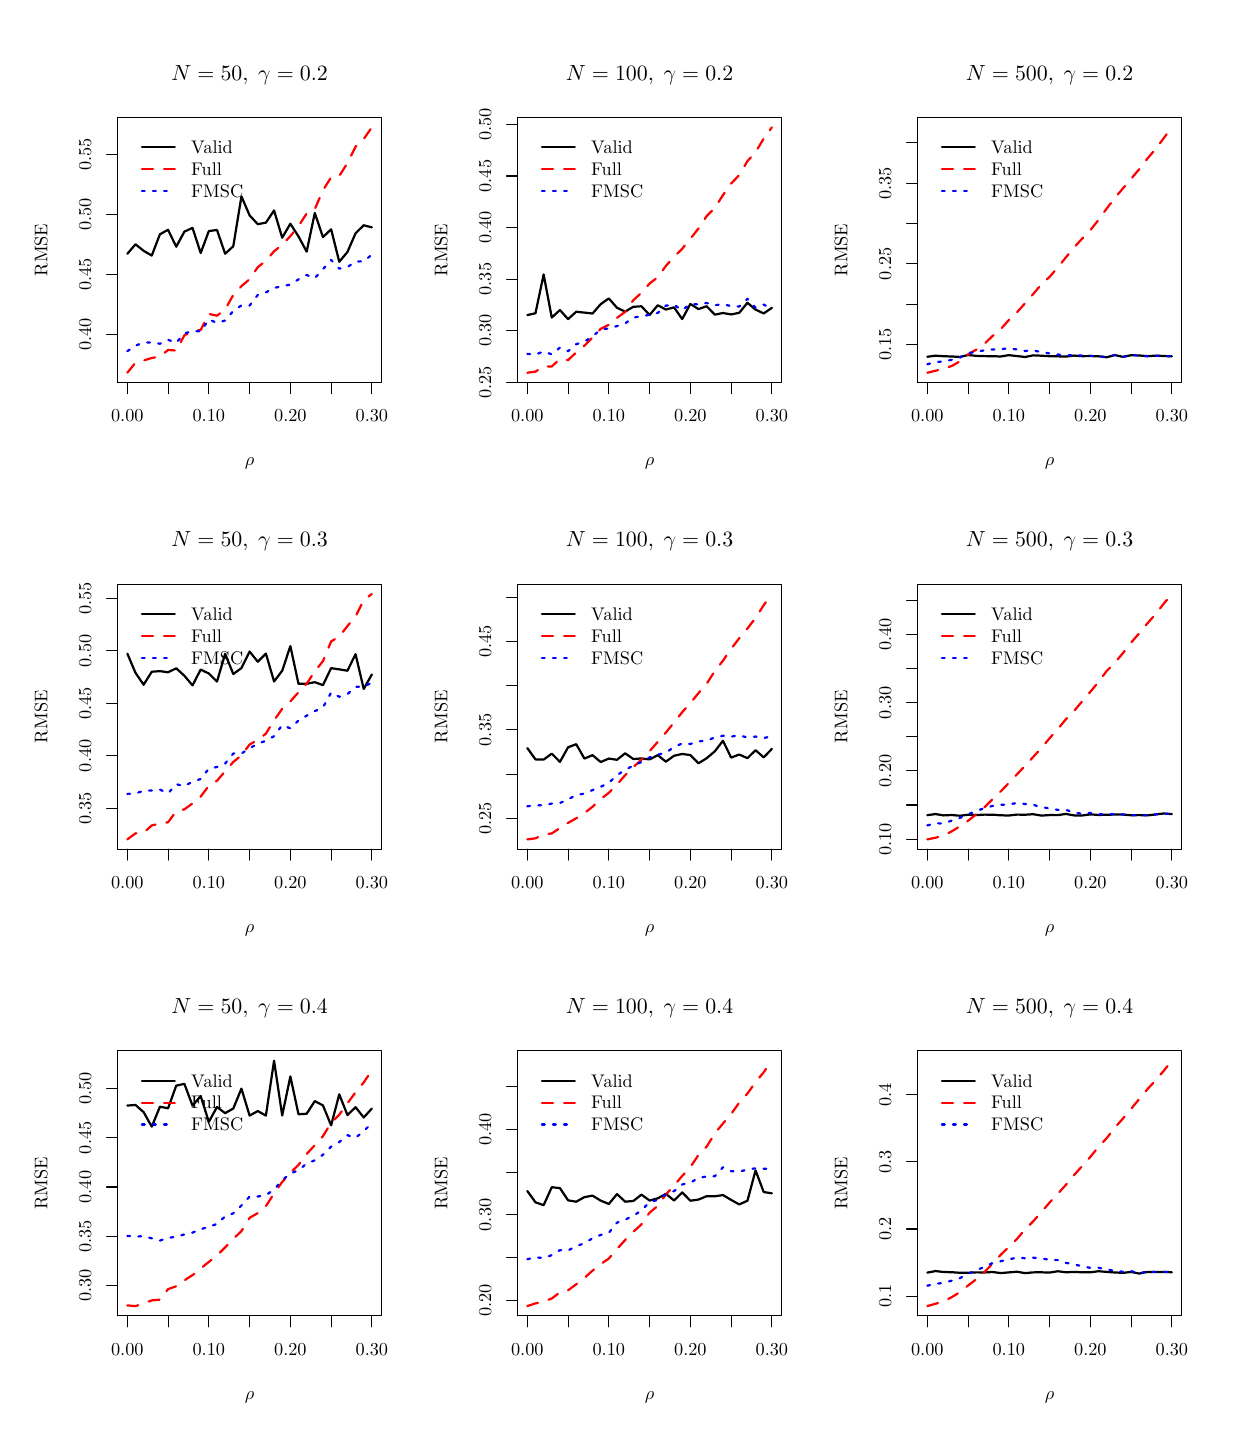
\begin{tikzpicture}[x=1pt,y=1pt]
\definecolor[named]{fillColor}{rgb}{1.00,1.00,1.00}
\path[use as bounding box,fill=fillColor,fill opacity=0.00] (0,0) rectangle (433.62,505.89);
\begin{scope}
\path[clip] ( 32.47,377.65) rectangle (127.91,473.42);
\definecolor[named]{drawColor}{rgb}{0.00,0.00,0.00}

\path[draw=drawColor,line width= 0.8pt,line join=round,line cap=round] ( 36.01,424.15) --
	( 38.95,427.61) --
	( 41.90,425.26) --
	( 44.84,423.54) --
	( 47.79,431.23) --
	( 50.73,432.85) --
	( 53.68,426.73) --
	( 56.63,432.19) --
	( 59.57,433.54) --
	( 62.52,424.45) --
	( 65.46,432.38) --
	( 68.41,432.79) --
	( 71.35,424.19) --
	( 74.30,426.91) --
	( 77.24,444.92) --
	( 80.19,438.07) --
	( 83.14,434.88) --
	( 86.08,435.43) --
	( 89.03,439.83) --
	( 91.97,430.00) --
	( 94.92,435.03) --
	( 97.86,430.45) --
	(100.81,424.95) --
	(103.75,438.92) --
	(106.70,430.21) --
	(109.65,433.03) --
	(112.59,421.28) --
	(115.54,424.82) --
	(118.48,431.58) --
	(121.43,434.49) --
	(124.37,433.72);
\end{scope}
\begin{scope}
\path[clip] (  0.00,  0.00) rectangle (433.62,505.89);
\definecolor[named]{drawColor}{rgb}{0.00,0.00,0.00}

\path[draw=drawColor,line width= 0.4pt,line join=round,line cap=round] ( 36.01,377.65) -- (124.37,377.65);

\path[draw=drawColor,line width= 0.4pt,line join=round,line cap=round] ( 36.01,377.65) -- ( 36.01,373.69);

\path[draw=drawColor,line width= 0.4pt,line join=round,line cap=round] ( 50.73,377.65) -- ( 50.73,373.69);

\path[draw=drawColor,line width= 0.4pt,line join=round,line cap=round] ( 65.46,377.65) -- ( 65.46,373.69);

\path[draw=drawColor,line width= 0.4pt,line join=round,line cap=round] ( 80.19,377.65) -- ( 80.19,373.69);

\path[draw=drawColor,line width= 0.4pt,line join=round,line cap=round] ( 94.92,377.65) -- ( 94.92,373.69);

\path[draw=drawColor,line width= 0.4pt,line join=round,line cap=round] (109.65,377.65) -- (109.65,373.69);

\path[draw=drawColor,line width= 0.4pt,line join=round,line cap=round] (124.37,377.65) -- (124.37,373.69);

\node[text=drawColor,anchor=base,inner sep=0pt, outer sep=0pt, scale=  0.66] at ( 36.01,363.40) {0.00};

\node[text=drawColor,anchor=base,inner sep=0pt, outer sep=0pt, scale=  0.66] at ( 65.46,363.40) {0.10};

\node[text=drawColor,anchor=base,inner sep=0pt, outer sep=0pt, scale=  0.66] at ( 94.92,363.40) {0.20};

\node[text=drawColor,anchor=base,inner sep=0pt, outer sep=0pt, scale=  0.66] at (124.37,363.40) {0.30};

\path[draw=drawColor,line width= 0.4pt,line join=round,line cap=round] ( 32.47,394.97) -- ( 32.47,460.08);

\path[draw=drawColor,line width= 0.4pt,line join=round,line cap=round] ( 32.47,394.97) -- ( 28.51,394.97);

\path[draw=drawColor,line width= 0.4pt,line join=round,line cap=round] ( 32.47,416.68) -- ( 28.51,416.68);

\path[draw=drawColor,line width= 0.4pt,line join=round,line cap=round] ( 32.47,438.38) -- ( 28.51,438.38);

\path[draw=drawColor,line width= 0.4pt,line join=round,line cap=round] ( 32.47,460.08) -- ( 28.51,460.08);

\node[text=drawColor,rotate= 90.00,anchor=base,inner sep=0pt, outer sep=0pt, scale=  0.66] at ( 22.97,394.97) {0.40};

\node[text=drawColor,rotate= 90.00,anchor=base,inner sep=0pt, outer sep=0pt, scale=  0.66] at ( 22.97,416.68) {0.45};

\node[text=drawColor,rotate= 90.00,anchor=base,inner sep=0pt, outer sep=0pt, scale=  0.66] at ( 22.97,438.38) {0.50};

\node[text=drawColor,rotate= 90.00,anchor=base,inner sep=0pt, outer sep=0pt, scale=  0.66] at ( 22.97,460.08) {0.55};

\path[draw=drawColor,line width= 0.4pt,line join=round,line cap=round] ( 32.47,377.65) --
	(127.91,377.65) --
	(127.91,473.42) --
	( 32.47,473.42) --
	( 32.47,377.65);
\end{scope}
\begin{scope}
\path[clip] (  0.00,337.26) rectangle (144.54,505.89);
\definecolor[named]{drawColor}{rgb}{0.00,0.00,0.00}

\node[text=drawColor,anchor=base,inner sep=0pt, outer sep=0pt, scale=  0.79] at ( 80.19,486.92) {\bfseries $N=50, \;\gamma=0.2$};

\node[text=drawColor,anchor=base,inner sep=0pt, outer sep=0pt, scale=  0.66] at ( 80.19,347.56) {$\rho$};

\node[text=drawColor,rotate= 90.00,anchor=base,inner sep=0pt, outer sep=0pt, scale=  0.66] at (  7.13,425.53) {RMSE};
\end{scope}
\begin{scope}
\path[clip] ( 32.47,377.65) rectangle (127.91,473.42);
\definecolor[named]{drawColor}{rgb}{1.00,0.00,0.00}

\path[draw=drawColor,line width= 0.8pt,dash pattern=on 4pt off 4pt ,line join=round,line cap=round] ( 36.01,381.20) --
	( 38.95,384.82) --
	( 41.90,385.63) --
	( 44.84,386.53) --
	( 47.79,387.02) --
	( 50.73,389.43) --
	( 53.68,389.21) --
	( 56.63,394.72) --
	( 59.57,396.22) --
	( 62.52,396.63) --
	( 65.46,402.46) --
	( 68.41,401.81) --
	( 71.35,404.07) --
	( 74.30,409.29) --
	( 77.24,412.47) --
	( 80.19,414.99) --
	( 83.14,419.35) --
	( 86.08,421.65) --
	( 89.03,425.08) --
	( 91.97,427.42) --
	( 94.92,430.56) --
	( 97.86,434.17) --
	(100.81,438.75) --
	(103.75,440.32) --
	(106.70,447.14) --
	(109.65,451.81) --
	(112.59,452.27) --
	(115.54,456.97) --
	(118.48,462.88) --
	(121.43,465.66) --
	(124.37,469.87);
\definecolor[named]{drawColor}{rgb}{0.00,0.00,1.00}

\path[draw=drawColor,line width= 0.8pt,dash pattern=on 1pt off 3pt ,line join=round,line cap=round] ( 36.01,388.99) --
	( 38.95,390.97) --
	( 41.90,392.10) --
	( 44.84,392.17) --
	( 47.79,391.68) --
	( 50.73,393.09) --
	( 53.68,392.01) --
	( 56.63,395.37) --
	( 59.57,396.31) --
	( 62.52,396.11) --
	( 65.46,400.43) --
	( 68.41,399.21) --
	( 71.35,400.06) --
	( 74.30,403.53) --
	( 77.24,405.51) --
	( 80.19,405.47) --
	( 83.14,409.29) --
	( 86.08,410.22) --
	( 89.03,411.89) --
	( 91.97,412.38) --
	( 94.92,413.08) --
	( 97.86,414.92) --
	(100.81,416.51) --
	(103.75,415.38) --
	(106.70,418.59) --
	(109.65,421.96) --
	(112.59,418.82) --
	(115.54,419.37) --
	(118.48,421.38) --
	(121.43,421.48) --
	(124.37,423.84);
\definecolor[named]{drawColor}{rgb}{0.00,0.00,0.00}

\path[draw=drawColor,line width= 0.8pt,line join=round,line cap=round] ( 41.28,462.63) -- ( 53.16,462.63);
\definecolor[named]{drawColor}{rgb}{1.00,0.00,0.00}

\path[draw=drawColor,line width= 0.8pt,dash pattern=on 4pt off 4pt ,line join=round,line cap=round] ( 41.28,454.71) -- ( 53.16,454.71);
\definecolor[named]{drawColor}{rgb}{0.00,0.00,1.00}

\path[draw=drawColor,line width= 0.8pt,dash pattern=on 1pt off 3pt ,line join=round,line cap=round] ( 41.28,446.79) -- ( 53.16,446.79);
\definecolor[named]{drawColor}{rgb}{0.00,0.00,0.00}

\node[text=drawColor,anchor=base west,inner sep=0pt, outer sep=0pt, scale=  0.66] at ( 59.10,460.35) {Valid};

\node[text=drawColor,anchor=base west,inner sep=0pt, outer sep=0pt, scale=  0.66] at ( 59.10,452.43) {Full};

\node[text=drawColor,anchor=base west,inner sep=0pt, outer sep=0pt, scale=  0.66] at ( 59.10,444.51) {FMSC};
\end{scope}
\begin{scope}
\path[clip] (177.01,377.65) rectangle (272.45,473.42);
\definecolor[named]{drawColor}{rgb}{0.00,0.00,0.00}

\path[draw=drawColor,line width= 0.8pt,line join=round,line cap=round] (180.55,402.03) --
	(183.49,402.69) --
	(186.44,416.70) --
	(189.38,401.13) --
	(192.33,403.85) --
	(195.27,400.57) --
	(198.22,403.24) --
	(201.17,402.93) --
	(204.11,402.60) --
	(207.06,405.98) --
	(210.00,408.05) --
	(212.95,404.67) --
	(215.89,403.28) --
	(218.84,405.02) --
	(221.78,405.21) --
	(224.73,402.06) --
	(227.68,405.58) --
	(230.62,404.03) --
	(233.57,404.82) --
	(236.51,400.59) --
	(239.46,406.05) --
	(242.40,404.20) --
	(245.35,405.23) --
	(248.29,402.19) --
	(251.24,402.77) --
	(254.19,402.27) --
	(257.13,402.86) --
	(260.08,406.47) --
	(263.02,404.02) --
	(265.97,402.62) --
	(268.91,404.65);
\end{scope}
\begin{scope}
\path[clip] (  0.00,  0.00) rectangle (433.62,505.89);
\definecolor[named]{drawColor}{rgb}{0.00,0.00,0.00}

\path[draw=drawColor,line width= 0.4pt,line join=round,line cap=round] (180.55,377.65) -- (268.91,377.65);

\path[draw=drawColor,line width= 0.4pt,line join=round,line cap=round] (180.55,377.65) -- (180.55,373.69);

\path[draw=drawColor,line width= 0.4pt,line join=round,line cap=round] (195.27,377.65) -- (195.27,373.69);

\path[draw=drawColor,line width= 0.4pt,line join=round,line cap=round] (210.00,377.65) -- (210.00,373.69);

\path[draw=drawColor,line width= 0.4pt,line join=round,line cap=round] (224.73,377.65) -- (224.73,373.69);

\path[draw=drawColor,line width= 0.4pt,line join=round,line cap=round] (239.46,377.65) -- (239.46,373.69);

\path[draw=drawColor,line width= 0.4pt,line join=round,line cap=round] (254.19,377.65) -- (254.19,373.69);

\path[draw=drawColor,line width= 0.4pt,line join=round,line cap=round] (268.91,377.65) -- (268.91,373.69);

\node[text=drawColor,anchor=base,inner sep=0pt, outer sep=0pt, scale=  0.66] at (180.55,363.40) {0.00};

\node[text=drawColor,anchor=base,inner sep=0pt, outer sep=0pt, scale=  0.66] at (210.00,363.40) {0.10};

\node[text=drawColor,anchor=base,inner sep=0pt, outer sep=0pt, scale=  0.66] at (239.46,363.40) {0.20};

\node[text=drawColor,anchor=base,inner sep=0pt, outer sep=0pt, scale=  0.66] at (268.91,363.40) {0.30};

\path[draw=drawColor,line width= 0.4pt,line join=round,line cap=round] (177.01,377.81) -- (177.01,470.89);

\path[draw=drawColor,line width= 0.4pt,line join=round,line cap=round] (177.01,377.81) -- (173.05,377.81);

\path[draw=drawColor,line width= 0.4pt,line join=round,line cap=round] (177.01,396.42) -- (173.05,396.42);

\path[draw=drawColor,line width= 0.4pt,line join=round,line cap=round] (177.01,415.04) -- (173.05,415.04);

\path[draw=drawColor,line width= 0.4pt,line join=round,line cap=round] (177.01,433.66) -- (173.05,433.66);

\path[draw=drawColor,line width= 0.4pt,line join=round,line cap=round] (177.01,452.27) -- (173.05,452.27);

\path[draw=drawColor,line width= 0.4pt,line join=round,line cap=round] (177.01,470.89) -- (173.05,470.89);

\node[text=drawColor,rotate= 90.00,anchor=base,inner sep=0pt, outer sep=0pt, scale=  0.66] at (167.51,377.81) {0.25};

\node[text=drawColor,rotate= 90.00,anchor=base,inner sep=0pt, outer sep=0pt, scale=  0.66] at (167.51,396.42) {0.30};

\node[text=drawColor,rotate= 90.00,anchor=base,inner sep=0pt, outer sep=0pt, scale=  0.66] at (167.51,415.04) {0.35};

\node[text=drawColor,rotate= 90.00,anchor=base,inner sep=0pt, outer sep=0pt, scale=  0.66] at (167.51,433.66) {0.40};

\node[text=drawColor,rotate= 90.00,anchor=base,inner sep=0pt, outer sep=0pt, scale=  0.66] at (167.51,452.27) {0.45};

\node[text=drawColor,rotate= 90.00,anchor=base,inner sep=0pt, outer sep=0pt, scale=  0.66] at (167.51,470.89) {0.50};

\path[draw=drawColor,line width= 0.4pt,line join=round,line cap=round] (177.01,377.65) --
	(272.45,377.65) --
	(272.45,473.42) --
	(177.01,473.42) --
	(177.01,377.65);
\end{scope}
\begin{scope}
\path[clip] (144.54,337.26) rectangle (289.08,505.89);
\definecolor[named]{drawColor}{rgb}{0.00,0.00,0.00}

\node[text=drawColor,anchor=base,inner sep=0pt, outer sep=0pt, scale=  0.79] at (224.73,486.92) {\bfseries $N=100, \;\gamma=0.2$};

\node[text=drawColor,anchor=base,inner sep=0pt, outer sep=0pt, scale=  0.66] at (224.73,347.56) {$\rho$};

\node[text=drawColor,rotate= 90.00,anchor=base,inner sep=0pt, outer sep=0pt, scale=  0.66] at (151.67,425.53) {RMSE};
\end{scope}
\begin{scope}
\path[clip] (177.01,377.65) rectangle (272.45,473.42);
\definecolor[named]{drawColor}{rgb}{1.00,0.00,0.00}

\path[draw=drawColor,line width= 0.8pt,dash pattern=on 4pt off 4pt ,line join=round,line cap=round] (180.55,381.20) --
	(183.49,381.58) --
	(186.44,383.54) --
	(189.38,383.44) --
	(192.33,386.21) --
	(195.27,385.76) --
	(198.22,388.57) --
	(201.17,390.96) --
	(204.11,393.95) --
	(207.06,397.06) --
	(210.00,398.51) --
	(212.95,401.03) --
	(215.89,403.20) --
	(218.84,407.40) --
	(221.78,410.07) --
	(224.73,413.43) --
	(227.68,415.73) --
	(230.62,419.81) --
	(233.57,423.09) --
	(236.51,425.98) --
	(239.46,429.63) --
	(242.40,433.31) --
	(245.35,437.80) --
	(248.29,440.75) --
	(251.24,445.38) --
	(254.19,449.54) --
	(257.13,452.66) --
	(260.08,457.65) --
	(263.02,460.92) --
	(265.97,465.81) --
	(268.91,469.87);
\definecolor[named]{drawColor}{rgb}{0.00,0.00,1.00}

\path[draw=drawColor,line width= 0.8pt,dash pattern=on 1pt off 3pt ,line join=round,line cap=round] (180.55,388.00) --
	(183.49,387.77) --
	(186.44,388.89) --
	(189.38,387.83) --
	(192.33,390.28) --
	(195.27,388.99) --
	(198.22,391.51) --
	(201.17,392.44) --
	(204.11,394.33) --
	(207.06,396.81) --
	(210.00,397.22) --
	(212.95,398.05) --
	(215.89,399.02) --
	(218.84,401.12) --
	(221.78,401.60) --
	(224.73,402.12) --
	(227.68,402.81) --
	(230.62,405.46) --
	(233.57,405.72) --
	(236.51,403.76) --
	(239.46,406.11) --
	(242.40,405.85) --
	(245.35,406.41) --
	(248.29,405.56) --
	(251.24,406.04) --
	(254.19,405.23) --
	(257.13,405.15) --
	(260.08,407.91) --
	(263.02,404.68) --
	(265.97,405.82) --
	(268.91,404.25);
\definecolor[named]{drawColor}{rgb}{0.00,0.00,0.00}

\path[draw=drawColor,line width= 0.8pt,line join=round,line cap=round] (185.82,462.63) -- (197.70,462.63);
\definecolor[named]{drawColor}{rgb}{1.00,0.00,0.00}

\path[draw=drawColor,line width= 0.8pt,dash pattern=on 4pt off 4pt ,line join=round,line cap=round] (185.82,454.71) -- (197.70,454.71);
\definecolor[named]{drawColor}{rgb}{0.00,0.00,1.00}

\path[draw=drawColor,line width= 0.8pt,dash pattern=on 1pt off 3pt ,line join=round,line cap=round] (185.82,446.79) -- (197.70,446.79);
\definecolor[named]{drawColor}{rgb}{0.00,0.00,0.00}

\node[text=drawColor,anchor=base west,inner sep=0pt, outer sep=0pt, scale=  0.66] at (203.64,460.35) {Valid};

\node[text=drawColor,anchor=base west,inner sep=0pt, outer sep=0pt, scale=  0.66] at (203.64,452.43) {Full};

\node[text=drawColor,anchor=base west,inner sep=0pt, outer sep=0pt, scale=  0.66] at (203.64,444.51) {FMSC};
\end{scope}
\begin{scope}
\path[clip] (321.55,377.65) rectangle (416.99,473.42);
\definecolor[named]{drawColor}{rgb}{0.00,0.00,0.00}

\path[draw=drawColor,line width= 0.8pt,line join=round,line cap=round] (325.09,386.97) --
	(328.03,387.36) --
	(330.98,387.16) --
	(333.92,387.07) --
	(336.87,386.91) --
	(339.81,387.59) --
	(342.76,387.30) --
	(345.71,387.20) --
	(348.65,387.17) --
	(351.60,387.07) --
	(354.54,387.55) --
	(357.49,387.22) --
	(360.43,386.89) --
	(363.38,387.48) --
	(366.32,387.35) --
	(369.27,387.16) --
	(372.22,387.12) --
	(375.16,387.03) --
	(378.11,387.39) --
	(381.05,387.18) --
	(384.00,387.22) --
	(386.94,387.14) --
	(389.89,386.78) --
	(392.83,387.58) --
	(395.78,386.93) --
	(398.73,387.53) --
	(401.67,387.43) --
	(404.62,387.18) --
	(407.56,387.37) --
	(410.51,387.24) --
	(413.45,387.13);
\end{scope}
\begin{scope}
\path[clip] (  0.00,  0.00) rectangle (433.62,505.89);
\definecolor[named]{drawColor}{rgb}{0.00,0.00,0.00}

\path[draw=drawColor,line width= 0.4pt,line join=round,line cap=round] (325.09,377.65) -- (413.45,377.65);

\path[draw=drawColor,line width= 0.4pt,line join=round,line cap=round] (325.09,377.65) -- (325.09,373.69);

\path[draw=drawColor,line width= 0.4pt,line join=round,line cap=round] (339.81,377.65) -- (339.81,373.69);

\path[draw=drawColor,line width= 0.4pt,line join=round,line cap=round] (354.54,377.65) -- (354.54,373.69);

\path[draw=drawColor,line width= 0.4pt,line join=round,line cap=round] (369.27,377.65) -- (369.27,373.69);

\path[draw=drawColor,line width= 0.4pt,line join=round,line cap=round] (384.00,377.65) -- (384.00,373.69);

\path[draw=drawColor,line width= 0.4pt,line join=round,line cap=round] (398.73,377.65) -- (398.73,373.69);

\path[draw=drawColor,line width= 0.4pt,line join=round,line cap=round] (413.45,377.65) -- (413.45,373.69);

\node[text=drawColor,anchor=base,inner sep=0pt, outer sep=0pt, scale=  0.66] at (325.09,363.40) {0.00};

\node[text=drawColor,anchor=base,inner sep=0pt, outer sep=0pt, scale=  0.66] at (354.54,363.40) {0.10};

\node[text=drawColor,anchor=base,inner sep=0pt, outer sep=0pt, scale=  0.66] at (384.00,363.40) {0.20};

\node[text=drawColor,anchor=base,inner sep=0pt, outer sep=0pt, scale=  0.66] at (413.45,363.40) {0.30};

\path[draw=drawColor,line width= 0.4pt,line join=round,line cap=round] (321.55,391.42) -- (321.55,464.29);

\path[draw=drawColor,line width= 0.4pt,line join=round,line cap=round] (321.55,391.42) -- (317.59,391.42);

\path[draw=drawColor,line width= 0.4pt,line join=round,line cap=round] (321.55,405.99) -- (317.59,405.99);

\path[draw=drawColor,line width= 0.4pt,line join=round,line cap=round] (321.55,420.57) -- (317.59,420.57);

\path[draw=drawColor,line width= 0.4pt,line join=round,line cap=round] (321.55,435.14) -- (317.59,435.14);

\path[draw=drawColor,line width= 0.4pt,line join=round,line cap=round] (321.55,449.71) -- (317.59,449.71);

\path[draw=drawColor,line width= 0.4pt,line join=round,line cap=round] (321.55,464.29) -- (317.59,464.29);

\node[text=drawColor,rotate= 90.00,anchor=base,inner sep=0pt, outer sep=0pt, scale=  0.66] at (312.05,391.42) {0.15};

\node[text=drawColor,rotate= 90.00,anchor=base,inner sep=0pt, outer sep=0pt, scale=  0.66] at (312.05,420.57) {0.25};

\node[text=drawColor,rotate= 90.00,anchor=base,inner sep=0pt, outer sep=0pt, scale=  0.66] at (312.05,449.71) {0.35};

\path[draw=drawColor,line width= 0.4pt,line join=round,line cap=round] (321.55,377.65) --
	(416.99,377.65) --
	(416.99,473.42) --
	(321.55,473.42) --
	(321.55,377.65);
\end{scope}
\begin{scope}
\path[clip] (289.08,337.26) rectangle (433.62,505.89);
\definecolor[named]{drawColor}{rgb}{0.00,0.00,0.00}

\node[text=drawColor,anchor=base,inner sep=0pt, outer sep=0pt, scale=  0.79] at (369.27,486.92) {\bfseries $N=500, \;\gamma=0.2$};

\node[text=drawColor,anchor=base,inner sep=0pt, outer sep=0pt, scale=  0.66] at (369.27,347.56) {$\rho$};

\node[text=drawColor,rotate= 90.00,anchor=base,inner sep=0pt, outer sep=0pt, scale=  0.66] at (296.21,425.53) {RMSE};
\end{scope}
\begin{scope}
\path[clip] (321.55,377.65) rectangle (416.99,473.42);
\definecolor[named]{drawColor}{rgb}{1.00,0.00,0.00}

\path[draw=drawColor,line width= 0.8pt,dash pattern=on 4pt off 4pt ,line join=round,line cap=round] (325.09,381.20) --
	(328.03,381.90) --
	(330.98,382.64) --
	(333.92,383.64) --
	(336.87,385.33) --
	(339.81,387.85) --
	(342.76,389.53) --
	(345.71,391.62) --
	(348.65,394.48) --
	(351.60,396.91) --
	(354.54,400.25) --
	(357.49,403.07) --
	(360.43,406.33) --
	(363.38,409.68) --
	(366.32,413.18) --
	(369.27,415.82) --
	(372.22,419.24) --
	(375.16,422.89) --
	(378.11,426.44) --
	(381.05,429.68) --
	(384.00,432.72) --
	(386.94,436.41) --
	(389.89,440.52) --
	(392.83,444.32) --
	(395.78,447.82) --
	(398.73,451.30) --
	(401.67,454.76) --
	(404.62,458.59) --
	(407.56,462.04) --
	(410.51,465.97) --
	(413.45,469.87);
\definecolor[named]{drawColor}{rgb}{0.00,0.00,1.00}

\path[draw=drawColor,line width= 0.8pt,dash pattern=on 1pt off 3pt ,line join=round,line cap=round] (325.09,384.27) --
	(328.03,385.01) --
	(330.98,385.31) --
	(333.92,385.85) --
	(336.87,386.72) --
	(339.81,388.28) --
	(342.76,388.72) --
	(345.71,389.31) --
	(348.65,389.60) --
	(351.60,389.66) --
	(354.54,390.10) --
	(357.49,389.58) --
	(360.43,389.08) --
	(363.38,389.20) --
	(366.32,388.69) --
	(369.27,388.16) --
	(372.22,387.78) --
	(375.16,387.40) --
	(378.11,387.66) --
	(381.05,387.39) --
	(384.00,387.30) --
	(386.94,387.20) --
	(389.89,386.79) --
	(392.83,387.59) --
	(395.78,386.93) --
	(398.73,387.53) --
	(401.67,387.43) --
	(404.62,387.18) --
	(407.56,387.37) --
	(410.51,387.24) --
	(413.45,387.13);
\definecolor[named]{drawColor}{rgb}{0.00,0.00,0.00}

\path[draw=drawColor,line width= 0.8pt,line join=round,line cap=round] (330.36,462.63) -- (342.24,462.63);
\definecolor[named]{drawColor}{rgb}{1.00,0.00,0.00}

\path[draw=drawColor,line width= 0.8pt,dash pattern=on 4pt off 4pt ,line join=round,line cap=round] (330.36,454.71) -- (342.24,454.71);
\definecolor[named]{drawColor}{rgb}{0.00,0.00,1.00}

\path[draw=drawColor,line width= 0.8pt,dash pattern=on 1pt off 3pt ,line join=round,line cap=round] (330.36,446.79) -- (342.24,446.79);
\definecolor[named]{drawColor}{rgb}{0.00,0.00,0.00}

\node[text=drawColor,anchor=base west,inner sep=0pt, outer sep=0pt, scale=  0.66] at (348.18,460.35) {Valid};

\node[text=drawColor,anchor=base west,inner sep=0pt, outer sep=0pt, scale=  0.66] at (348.18,452.43) {Full};

\node[text=drawColor,anchor=base west,inner sep=0pt, outer sep=0pt, scale=  0.66] at (348.18,444.51) {FMSC};
\end{scope}
\begin{scope}
\path[clip] ( 32.47,209.02) rectangle (127.91,304.79);
\definecolor[named]{drawColor}{rgb}{0.00,0.00,0.00}

\path[draw=drawColor,line width= 0.8pt,line join=round,line cap=round] ( 36.01,279.71) --
	( 38.95,272.76) --
	( 41.90,268.46) --
	( 44.84,273.16) --
	( 47.79,273.37) --
	( 50.73,272.95) --
	( 53.68,274.40) --
	( 56.63,271.70) --
	( 59.57,268.22) --
	( 62.52,273.95) --
	( 65.46,272.51) --
	( 68.41,269.58) --
	( 71.35,279.63) --
	( 74.30,272.32) --
	( 77.24,274.48) --
	( 80.19,280.45) --
	( 83.14,276.77) --
	( 86.08,279.72) --
	( 89.03,269.63) --
	( 91.97,273.52) --
	( 94.92,282.41) --
	( 97.86,268.78) --
	(100.81,268.81) --
	(103.75,269.38) --
	(106.70,268.32) --
	(109.65,274.45) --
	(112.59,274.01) --
	(115.54,273.52) --
	(118.48,279.49) --
	(121.43,266.94) --
	(124.37,272.17);
\end{scope}
\begin{scope}
\path[clip] (  0.00,  0.00) rectangle (433.62,505.89);
\definecolor[named]{drawColor}{rgb}{0.00,0.00,0.00}

\path[draw=drawColor,line width= 0.4pt,line join=round,line cap=round] ( 36.01,209.02) -- (124.37,209.02);

\path[draw=drawColor,line width= 0.4pt,line join=round,line cap=round] ( 36.01,209.02) -- ( 36.01,205.06);

\path[draw=drawColor,line width= 0.4pt,line join=round,line cap=round] ( 50.73,209.02) -- ( 50.73,205.06);

\path[draw=drawColor,line width= 0.4pt,line join=round,line cap=round] ( 65.46,209.02) -- ( 65.46,205.06);

\path[draw=drawColor,line width= 0.4pt,line join=round,line cap=round] ( 80.19,209.02) -- ( 80.19,205.06);

\path[draw=drawColor,line width= 0.4pt,line join=round,line cap=round] ( 94.92,209.02) -- ( 94.92,205.06);

\path[draw=drawColor,line width= 0.4pt,line join=round,line cap=round] (109.65,209.02) -- (109.65,205.06);

\path[draw=drawColor,line width= 0.4pt,line join=round,line cap=round] (124.37,209.02) -- (124.37,205.06);

\node[text=drawColor,anchor=base,inner sep=0pt, outer sep=0pt, scale=  0.66] at ( 36.01,194.77) {0.00};

\node[text=drawColor,anchor=base,inner sep=0pt, outer sep=0pt, scale=  0.66] at ( 65.46,194.77) {0.10};

\node[text=drawColor,anchor=base,inner sep=0pt, outer sep=0pt, scale=  0.66] at ( 94.92,194.77) {0.20};

\node[text=drawColor,anchor=base,inner sep=0pt, outer sep=0pt, scale=  0.66] at (124.37,194.77) {0.30};

\path[draw=drawColor,line width= 0.4pt,line join=round,line cap=round] ( 32.47,223.84) -- ( 32.47,299.62);

\path[draw=drawColor,line width= 0.4pt,line join=round,line cap=round] ( 32.47,223.84) -- ( 28.51,223.84);

\path[draw=drawColor,line width= 0.4pt,line join=round,line cap=round] ( 32.47,242.79) -- ( 28.51,242.79);

\path[draw=drawColor,line width= 0.4pt,line join=round,line cap=round] ( 32.47,261.73) -- ( 28.51,261.73);

\path[draw=drawColor,line width= 0.4pt,line join=round,line cap=round] ( 32.47,280.67) -- ( 28.51,280.67);

\path[draw=drawColor,line width= 0.4pt,line join=round,line cap=round] ( 32.47,299.62) -- ( 28.51,299.62);

\node[text=drawColor,rotate= 90.00,anchor=base,inner sep=0pt, outer sep=0pt, scale=  0.66] at ( 22.97,223.84) {0.35};

\node[text=drawColor,rotate= 90.00,anchor=base,inner sep=0pt, outer sep=0pt, scale=  0.66] at ( 22.97,242.79) {0.40};

\node[text=drawColor,rotate= 90.00,anchor=base,inner sep=0pt, outer sep=0pt, scale=  0.66] at ( 22.97,261.73) {0.45};

\node[text=drawColor,rotate= 90.00,anchor=base,inner sep=0pt, outer sep=0pt, scale=  0.66] at ( 22.97,280.67) {0.50};

\node[text=drawColor,rotate= 90.00,anchor=base,inner sep=0pt, outer sep=0pt, scale=  0.66] at ( 22.97,299.62) {0.55};

\path[draw=drawColor,line width= 0.4pt,line join=round,line cap=round] ( 32.47,209.02) --
	(127.91,209.02) --
	(127.91,304.79) --
	( 32.47,304.79) --
	( 32.47,209.02);
\end{scope}
\begin{scope}
\path[clip] (  0.00,168.63) rectangle (144.54,337.26);
\definecolor[named]{drawColor}{rgb}{0.00,0.00,0.00}

\node[text=drawColor,anchor=base,inner sep=0pt, outer sep=0pt, scale=  0.79] at ( 80.19,318.29) {\bfseries $N=50, \;\gamma=0.3$};

\node[text=drawColor,anchor=base,inner sep=0pt, outer sep=0pt, scale=  0.66] at ( 80.19,178.93) {$\rho$};

\node[text=drawColor,rotate= 90.00,anchor=base,inner sep=0pt, outer sep=0pt, scale=  0.66] at (  7.13,256.90) {RMSE};
\end{scope}
\begin{scope}
\path[clip] ( 32.47,209.02) rectangle (127.91,304.79);
\definecolor[named]{drawColor}{rgb}{1.00,0.00,0.00}

\path[draw=drawColor,line width= 0.8pt,dash pattern=on 4pt off 4pt ,line join=round,line cap=round] ( 36.01,212.57) --
	( 38.95,214.75) --
	( 41.90,214.90) --
	( 44.84,217.63) --
	( 47.79,218.28) --
	( 50.73,218.75) --
	( 53.68,222.75) --
	( 56.63,223.43) --
	( 59.57,225.59) --
	( 62.52,228.05) --
	( 65.46,231.95) --
	( 68.41,233.76) --
	( 71.35,237.19) --
	( 74.30,240.56) --
	( 77.24,242.94) --
	( 80.19,246.86) --
	( 83.14,248.52) --
	( 86.08,250.79) --
	( 89.03,255.59) --
	( 91.97,259.76) --
	( 94.92,262.43) --
	( 97.86,265.74) --
	(100.81,268.82) --
	(103.75,273.30) --
	(106.70,276.98) --
	(109.65,284.09) --
	(112.59,285.89) --
	(115.54,289.65) --
	(118.48,293.08) --
	(121.43,299.01) --
	(124.37,301.24);
\definecolor[named]{drawColor}{rgb}{0.00,0.00,1.00}

\path[draw=drawColor,line width= 0.8pt,dash pattern=on 1pt off 3pt ,line join=round,line cap=round] ( 36.01,228.99) --
	( 38.95,229.22) --
	( 41.90,230.08) --
	( 44.84,230.24) --
	( 47.79,230.56) --
	( 50.73,229.22) --
	( 53.68,232.50) --
	( 56.63,231.84) --
	( 59.57,233.42) --
	( 62.52,234.39) --
	( 65.46,238.13) --
	( 68.41,238.74) --
	( 71.35,239.99) --
	( 74.30,243.59) --
	( 77.24,243.60) --
	( 80.19,245.51) --
	( 83.14,247.14) --
	( 86.08,248.20) --
	( 89.03,249.87) --
	( 91.97,253.86) --
	( 94.92,252.70) --
	( 97.86,255.53) --
	(100.81,257.28) --
	(103.75,258.92) --
	(106.70,260.25) --
	(109.65,265.62) --
	(112.59,264.11) --
	(115.54,265.05) --
	(118.48,267.68) --
	(121.43,267.82) --
	(124.37,269.14);
\definecolor[named]{drawColor}{rgb}{0.00,0.00,0.00}

\path[draw=drawColor,line width= 0.8pt,line join=round,line cap=round] ( 41.28,294.00) -- ( 53.16,294.00);
\definecolor[named]{drawColor}{rgb}{1.00,0.00,0.00}

\path[draw=drawColor,line width= 0.8pt,dash pattern=on 4pt off 4pt ,line join=round,line cap=round] ( 41.28,286.08) -- ( 53.16,286.08);
\definecolor[named]{drawColor}{rgb}{0.00,0.00,1.00}

\path[draw=drawColor,line width= 0.8pt,dash pattern=on 1pt off 3pt ,line join=round,line cap=round] ( 41.28,278.16) -- ( 53.16,278.16);
\definecolor[named]{drawColor}{rgb}{0.00,0.00,0.00}

\node[text=drawColor,anchor=base west,inner sep=0pt, outer sep=0pt, scale=  0.66] at ( 59.10,291.72) {Valid};

\node[text=drawColor,anchor=base west,inner sep=0pt, outer sep=0pt, scale=  0.66] at ( 59.10,283.80) {Full};

\node[text=drawColor,anchor=base west,inner sep=0pt, outer sep=0pt, scale=  0.66] at ( 59.10,275.88) {FMSC};
\end{scope}
\begin{scope}
\path[clip] (177.01,209.02) rectangle (272.45,304.79);
\definecolor[named]{drawColor}{rgb}{0.00,0.00,0.00}

\path[draw=drawColor,line width= 0.8pt,line join=round,line cap=round] (180.55,245.57) --
	(183.49,241.48) --
	(186.44,241.41) --
	(189.38,243.55) --
	(192.33,240.58) --
	(195.27,245.86) --
	(198.22,246.97) --
	(201.17,241.78) --
	(204.11,243.01) --
	(207.06,240.53) --
	(210.00,241.78) --
	(212.95,241.33) --
	(215.89,243.69) --
	(218.84,241.62) --
	(221.78,241.81) --
	(224.73,241.48) --
	(227.68,243.01) --
	(230.62,240.66) --
	(233.57,242.80) --
	(236.51,243.44) --
	(239.46,243.04) --
	(242.40,240.08) --
	(245.35,241.90) --
	(248.29,244.40) --
	(251.24,248.20) --
	(254.19,242.13) --
	(257.13,243.23) --
	(260.08,241.93) --
	(263.02,244.80) --
	(265.97,242.20) --
	(268.91,245.28);
\end{scope}
\begin{scope}
\path[clip] (  0.00,  0.00) rectangle (433.62,505.89);
\definecolor[named]{drawColor}{rgb}{0.00,0.00,0.00}

\path[draw=drawColor,line width= 0.4pt,line join=round,line cap=round] (180.55,209.02) -- (268.91,209.02);

\path[draw=drawColor,line width= 0.4pt,line join=round,line cap=round] (180.55,209.02) -- (180.55,205.06);

\path[draw=drawColor,line width= 0.4pt,line join=round,line cap=round] (195.27,209.02) -- (195.27,205.06);

\path[draw=drawColor,line width= 0.4pt,line join=round,line cap=round] (210.00,209.02) -- (210.00,205.06);

\path[draw=drawColor,line width= 0.4pt,line join=round,line cap=round] (224.73,209.02) -- (224.73,205.06);

\path[draw=drawColor,line width= 0.4pt,line join=round,line cap=round] (239.46,209.02) -- (239.46,205.06);

\path[draw=drawColor,line width= 0.4pt,line join=round,line cap=round] (254.19,209.02) -- (254.19,205.06);

\path[draw=drawColor,line width= 0.4pt,line join=round,line cap=round] (268.91,209.02) -- (268.91,205.06);

\node[text=drawColor,anchor=base,inner sep=0pt, outer sep=0pt, scale=  0.66] at (180.55,194.77) {0.00};

\node[text=drawColor,anchor=base,inner sep=0pt, outer sep=0pt, scale=  0.66] at (210.00,194.77) {0.10};

\node[text=drawColor,anchor=base,inner sep=0pt, outer sep=0pt, scale=  0.66] at (239.46,194.77) {0.20};

\node[text=drawColor,anchor=base,inner sep=0pt, outer sep=0pt, scale=  0.66] at (268.91,194.77) {0.30};

\path[draw=drawColor,line width= 0.4pt,line join=round,line cap=round] (177.01,220.23) -- (177.01,299.96);

\path[draw=drawColor,line width= 0.4pt,line join=round,line cap=round] (177.01,220.23) -- (173.05,220.23);

\path[draw=drawColor,line width= 0.4pt,line join=round,line cap=round] (177.01,236.18) -- (173.05,236.18);

\path[draw=drawColor,line width= 0.4pt,line join=round,line cap=round] (177.01,252.13) -- (173.05,252.13);

\path[draw=drawColor,line width= 0.4pt,line join=round,line cap=round] (177.01,268.07) -- (173.05,268.07);

\path[draw=drawColor,line width= 0.4pt,line join=round,line cap=round] (177.01,284.02) -- (173.05,284.02);

\path[draw=drawColor,line width= 0.4pt,line join=round,line cap=round] (177.01,299.96) -- (173.05,299.96);

\node[text=drawColor,rotate= 90.00,anchor=base,inner sep=0pt, outer sep=0pt, scale=  0.66] at (167.51,220.23) {0.25};

\node[text=drawColor,rotate= 90.00,anchor=base,inner sep=0pt, outer sep=0pt, scale=  0.66] at (167.51,252.13) {0.35};

\node[text=drawColor,rotate= 90.00,anchor=base,inner sep=0pt, outer sep=0pt, scale=  0.66] at (167.51,284.02) {0.45};

\path[draw=drawColor,line width= 0.4pt,line join=round,line cap=round] (177.01,209.02) --
	(272.45,209.02) --
	(272.45,304.79) --
	(177.01,304.79) --
	(177.01,209.02);
\end{scope}
\begin{scope}
\path[clip] (144.54,168.63) rectangle (289.08,337.26);
\definecolor[named]{drawColor}{rgb}{0.00,0.00,0.00}

\node[text=drawColor,anchor=base,inner sep=0pt, outer sep=0pt, scale=  0.79] at (224.73,318.29) {\bfseries $N=100, \;\gamma=0.3$};

\node[text=drawColor,anchor=base,inner sep=0pt, outer sep=0pt, scale=  0.66] at (224.73,178.93) {$\rho$};

\node[text=drawColor,rotate= 90.00,anchor=base,inner sep=0pt, outer sep=0pt, scale=  0.66] at (151.67,256.90) {RMSE};
\end{scope}
\begin{scope}
\path[clip] (177.01,209.02) rectangle (272.45,304.79);
\definecolor[named]{drawColor}{rgb}{1.00,0.00,0.00}

\path[draw=drawColor,line width= 0.8pt,dash pattern=on 4pt off 4pt ,line join=round,line cap=round] (180.55,212.57) --
	(183.49,212.96) --
	(186.44,214.35) --
	(189.38,214.71) --
	(192.33,216.71) --
	(195.27,218.54) --
	(198.22,220.22) --
	(201.17,222.06) --
	(204.11,224.37) --
	(207.06,227.12) --
	(210.00,229.41) --
	(212.95,232.39) --
	(215.89,235.76) --
	(218.84,238.70) --
	(221.78,241.37) --
	(224.73,244.46) --
	(227.68,247.83) --
	(230.62,251.19) --
	(233.57,254.82) --
	(236.51,258.54) --
	(239.46,261.83) --
	(242.40,265.44) --
	(245.35,268.80) --
	(248.29,273.39) --
	(251.24,277.15) --
	(254.19,281.45) --
	(257.13,285.27) --
	(260.08,288.78) --
	(263.02,292.59) --
	(265.97,297.22) --
	(268.91,301.24);
\definecolor[named]{drawColor}{rgb}{0.00,0.00,1.00}

\path[draw=drawColor,line width= 0.8pt,dash pattern=on 1pt off 3pt ,line join=round,line cap=round] (180.55,224.53) --
	(183.49,224.88) --
	(186.44,224.92) --
	(189.38,225.50) --
	(192.33,225.72) --
	(195.27,227.03) --
	(198.22,228.62) --
	(201.17,229.12) --
	(204.11,230.39) --
	(207.06,231.58) --
	(210.00,233.02) --
	(212.95,235.76) --
	(215.89,237.75) --
	(218.84,239.18) --
	(221.78,240.55) --
	(224.73,242.19) --
	(227.68,243.19) --
	(230.62,243.91) --
	(233.57,245.94) --
	(236.51,247.26) --
	(239.46,247.06) --
	(242.40,247.98) --
	(245.35,248.31) --
	(248.29,249.40) --
	(251.24,250.03) --
	(254.19,249.71) --
	(257.13,250.19) --
	(260.08,249.38) --
	(263.02,249.73) --
	(265.97,249.16) --
	(268.91,249.93);
\definecolor[named]{drawColor}{rgb}{0.00,0.00,0.00}

\path[draw=drawColor,line width= 0.8pt,line join=round,line cap=round] (185.82,294.00) -- (197.70,294.00);
\definecolor[named]{drawColor}{rgb}{1.00,0.00,0.00}

\path[draw=drawColor,line width= 0.8pt,dash pattern=on 4pt off 4pt ,line join=round,line cap=round] (185.82,286.08) -- (197.70,286.08);
\definecolor[named]{drawColor}{rgb}{0.00,0.00,1.00}

\path[draw=drawColor,line width= 0.8pt,dash pattern=on 1pt off 3pt ,line join=round,line cap=round] (185.82,278.16) -- (197.70,278.16);
\definecolor[named]{drawColor}{rgb}{0.00,0.00,0.00}

\node[text=drawColor,anchor=base west,inner sep=0pt, outer sep=0pt, scale=  0.66] at (203.64,291.72) {Valid};

\node[text=drawColor,anchor=base west,inner sep=0pt, outer sep=0pt, scale=  0.66] at (203.64,283.80) {Full};

\node[text=drawColor,anchor=base west,inner sep=0pt, outer sep=0pt, scale=  0.66] at (203.64,275.88) {FMSC};
\end{scope}
\begin{scope}
\path[clip] (321.55,209.02) rectangle (416.99,304.79);
\definecolor[named]{drawColor}{rgb}{0.00,0.00,0.00}

\path[draw=drawColor,line width= 0.8pt,line join=round,line cap=round] (325.09,221.32) --
	(328.03,221.73) --
	(330.98,221.24) --
	(333.92,221.38) --
	(336.87,221.12) --
	(339.81,221.47) --
	(342.76,221.35) --
	(345.71,221.52) --
	(348.65,221.50) --
	(351.60,221.28) --
	(354.54,221.20) --
	(357.49,221.53) --
	(360.43,221.49) --
	(363.38,221.67) --
	(366.32,221.17) --
	(369.27,221.36) --
	(372.22,221.34) --
	(375.16,221.77) --
	(378.11,221.24) --
	(381.05,221.21) --
	(384.00,221.61) --
	(386.94,221.40) --
	(389.89,221.48) --
	(392.83,221.54) --
	(395.78,221.55) --
	(398.73,221.29) --
	(401.67,221.35) --
	(404.62,221.25) --
	(407.56,221.59) --
	(410.51,221.93) --
	(413.45,221.70);
\end{scope}
\begin{scope}
\path[clip] (  0.00,  0.00) rectangle (433.62,505.89);
\definecolor[named]{drawColor}{rgb}{0.00,0.00,0.00}

\path[draw=drawColor,line width= 0.4pt,line join=round,line cap=round] (325.09,209.02) -- (413.45,209.02);

\path[draw=drawColor,line width= 0.4pt,line join=round,line cap=round] (325.09,209.02) -- (325.09,205.06);

\path[draw=drawColor,line width= 0.4pt,line join=round,line cap=round] (339.81,209.02) -- (339.81,205.06);

\path[draw=drawColor,line width= 0.4pt,line join=round,line cap=round] (354.54,209.02) -- (354.54,205.06);

\path[draw=drawColor,line width= 0.4pt,line join=round,line cap=round] (369.27,209.02) -- (369.27,205.06);

\path[draw=drawColor,line width= 0.4pt,line join=round,line cap=round] (384.00,209.02) -- (384.00,205.06);

\path[draw=drawColor,line width= 0.4pt,line join=round,line cap=round] (398.73,209.02) -- (398.73,205.06);

\path[draw=drawColor,line width= 0.4pt,line join=round,line cap=round] (413.45,209.02) -- (413.45,205.06);

\node[text=drawColor,anchor=base,inner sep=0pt, outer sep=0pt, scale=  0.66] at (325.09,194.77) {0.00};

\node[text=drawColor,anchor=base,inner sep=0pt, outer sep=0pt, scale=  0.66] at (354.54,194.77) {0.10};

\node[text=drawColor,anchor=base,inner sep=0pt, outer sep=0pt, scale=  0.66] at (384.00,194.77) {0.20};

\node[text=drawColor,anchor=base,inner sep=0pt, outer sep=0pt, scale=  0.66] at (413.45,194.77) {0.30};

\path[draw=drawColor,line width= 0.4pt,line join=round,line cap=round] (321.55,212.68) -- (321.55,298.87);

\path[draw=drawColor,line width= 0.4pt,line join=round,line cap=round] (321.55,212.68) -- (317.59,212.68);

\path[draw=drawColor,line width= 0.4pt,line join=round,line cap=round] (321.55,224.99) -- (317.59,224.99);

\path[draw=drawColor,line width= 0.4pt,line join=round,line cap=round] (321.55,237.31) -- (317.59,237.31);

\path[draw=drawColor,line width= 0.4pt,line join=round,line cap=round] (321.55,249.62) -- (317.59,249.62);

\path[draw=drawColor,line width= 0.4pt,line join=round,line cap=round] (321.55,261.93) -- (317.59,261.93);

\path[draw=drawColor,line width= 0.4pt,line join=round,line cap=round] (321.55,274.25) -- (317.59,274.25);

\path[draw=drawColor,line width= 0.4pt,line join=round,line cap=round] (321.55,286.56) -- (317.59,286.56);

\path[draw=drawColor,line width= 0.4pt,line join=round,line cap=round] (321.55,298.87) -- (317.59,298.87);

\node[text=drawColor,rotate= 90.00,anchor=base,inner sep=0pt, outer sep=0pt, scale=  0.66] at (312.05,212.68) {0.10};

\node[text=drawColor,rotate= 90.00,anchor=base,inner sep=0pt, outer sep=0pt, scale=  0.66] at (312.05,237.31) {0.20};

\node[text=drawColor,rotate= 90.00,anchor=base,inner sep=0pt, outer sep=0pt, scale=  0.66] at (312.05,261.93) {0.30};

\node[text=drawColor,rotate= 90.00,anchor=base,inner sep=0pt, outer sep=0pt, scale=  0.66] at (312.05,286.56) {0.40};

\path[draw=drawColor,line width= 0.4pt,line join=round,line cap=round] (321.55,209.02) --
	(416.99,209.02) --
	(416.99,304.79) --
	(321.55,304.79) --
	(321.55,209.02);
\end{scope}
\begin{scope}
\path[clip] (289.08,168.63) rectangle (433.62,337.26);
\definecolor[named]{drawColor}{rgb}{0.00,0.00,0.00}

\node[text=drawColor,anchor=base,inner sep=0pt, outer sep=0pt, scale=  0.79] at (369.27,318.29) {\bfseries $N=500, \;\gamma=0.3$};

\node[text=drawColor,anchor=base,inner sep=0pt, outer sep=0pt, scale=  0.66] at (369.27,178.93) {$\rho$};

\node[text=drawColor,rotate= 90.00,anchor=base,inner sep=0pt, outer sep=0pt, scale=  0.66] at (296.21,256.90) {RMSE};
\end{scope}
\begin{scope}
\path[clip] (321.55,209.02) rectangle (416.99,304.79);
\definecolor[named]{drawColor}{rgb}{1.00,0.00,0.00}

\path[draw=drawColor,line width= 0.8pt,dash pattern=on 4pt off 4pt ,line join=round,line cap=round] (325.09,212.57) --
	(328.03,213.16) --
	(330.98,213.98) --
	(333.92,215.49) --
	(336.87,217.31) --
	(339.81,219.31) --
	(342.76,221.63) --
	(345.71,224.15) --
	(348.65,227.08) --
	(351.60,229.89) --
	(354.54,232.95) --
	(357.49,236.08) --
	(360.43,239.20) --
	(363.38,242.41) --
	(366.32,245.61) --
	(369.27,249.12) --
	(372.22,252.41) --
	(375.16,255.99) --
	(378.11,258.99) --
	(381.05,262.48) --
	(384.00,265.92) --
	(386.94,269.47) --
	(389.89,273.43) --
	(392.83,276.41) --
	(395.78,279.88) --
	(398.73,283.71) --
	(401.67,287.07) --
	(404.62,290.65) --
	(407.56,293.95) --
	(410.51,297.75) --
	(413.45,301.24);
\definecolor[named]{drawColor}{rgb}{0.00,0.00,1.00}

\path[draw=drawColor,line width= 0.8pt,dash pattern=on 1pt off 3pt ,line join=round,line cap=round] (325.09,217.62) --
	(328.03,218.39) --
	(330.98,218.32) --
	(333.92,219.36) --
	(336.87,220.33) --
	(339.81,221.65) --
	(342.76,222.75) --
	(345.71,223.92) --
	(348.65,224.65) --
	(351.60,225.07) --
	(354.54,225.20) --
	(357.49,225.73) --
	(360.43,225.36) --
	(363.38,225.08) --
	(366.32,224.17) --
	(369.27,223.79) --
	(372.22,223.23) --
	(375.16,223.27) --
	(378.11,222.21) --
	(381.05,221.87) --
	(384.00,222.12) --
	(386.94,221.69) --
	(389.89,221.65) --
	(392.83,221.64) --
	(395.78,221.59) --
	(398.73,221.32) --
	(401.67,221.37) --
	(404.62,221.26) --
	(407.56,221.60) --
	(410.51,221.93) --
	(413.45,221.70);
\definecolor[named]{drawColor}{rgb}{0.00,0.00,0.00}

\path[draw=drawColor,line width= 0.8pt,line join=round,line cap=round] (330.36,294.00) -- (342.24,294.00);
\definecolor[named]{drawColor}{rgb}{1.00,0.00,0.00}

\path[draw=drawColor,line width= 0.8pt,dash pattern=on 4pt off 4pt ,line join=round,line cap=round] (330.36,286.08) -- (342.24,286.08);
\definecolor[named]{drawColor}{rgb}{0.00,0.00,1.00}

\path[draw=drawColor,line width= 0.8pt,dash pattern=on 1pt off 3pt ,line join=round,line cap=round] (330.36,278.16) -- (342.24,278.16);
\definecolor[named]{drawColor}{rgb}{0.00,0.00,0.00}

\node[text=drawColor,anchor=base west,inner sep=0pt, outer sep=0pt, scale=  0.66] at (348.18,291.72) {Valid};

\node[text=drawColor,anchor=base west,inner sep=0pt, outer sep=0pt, scale=  0.66] at (348.18,283.80) {Full};

\node[text=drawColor,anchor=base west,inner sep=0pt, outer sep=0pt, scale=  0.66] at (348.18,275.88) {FMSC};
\end{scope}
\begin{scope}
\path[clip] ( 32.47, 40.39) rectangle (127.91,136.16);
\definecolor[named]{drawColor}{rgb}{0.00,0.00,0.00}

\path[draw=drawColor,line width= 0.8pt,line join=round,line cap=round] ( 36.01,116.39) --
	( 38.95,116.61) --
	( 41.90,114.01) --
	( 44.84,108.78) --
	( 47.79,115.97) --
	( 50.73,115.41) --
	( 53.68,123.58) --
	( 56.63,124.25) --
	( 59.57,116.36) --
	( 62.52,119.83) --
	( 65.46,110.50) --
	( 68.41,115.88) --
	( 71.35,113.65) --
	( 74.30,115.33) --
	( 77.24,122.52) --
	( 80.19,112.77) --
	( 83.14,114.40) --
	( 86.08,112.78) --
	( 89.03,132.61) --
	( 91.97,112.80) --
	( 94.92,126.92) --
	( 97.86,113.26) --
	(100.81,113.43) --
	(103.75,118.00) --
	(106.70,116.45) --
	(109.65,109.23) --
	(112.59,120.46) --
	(115.54,112.97) --
	(118.48,115.80) --
	(121.43,112.08) --
	(124.37,115.32);
\end{scope}
\begin{scope}
\path[clip] (  0.00,  0.00) rectangle (433.62,505.89);
\definecolor[named]{drawColor}{rgb}{0.00,0.00,0.00}

\path[draw=drawColor,line width= 0.4pt,line join=round,line cap=round] ( 36.01, 40.39) -- (124.37, 40.39);

\path[draw=drawColor,line width= 0.4pt,line join=round,line cap=round] ( 36.01, 40.39) -- ( 36.01, 36.43);

\path[draw=drawColor,line width= 0.4pt,line join=round,line cap=round] ( 50.73, 40.39) -- ( 50.73, 36.43);

\path[draw=drawColor,line width= 0.4pt,line join=round,line cap=round] ( 65.46, 40.39) -- ( 65.46, 36.43);

\path[draw=drawColor,line width= 0.4pt,line join=round,line cap=round] ( 80.19, 40.39) -- ( 80.19, 36.43);

\path[draw=drawColor,line width= 0.4pt,line join=round,line cap=round] ( 94.92, 40.39) -- ( 94.92, 36.43);

\path[draw=drawColor,line width= 0.4pt,line join=round,line cap=round] (109.65, 40.39) -- (109.65, 36.43);

\path[draw=drawColor,line width= 0.4pt,line join=round,line cap=round] (124.37, 40.39) -- (124.37, 36.43);

\node[text=drawColor,anchor=base,inner sep=0pt, outer sep=0pt, scale=  0.66] at ( 36.01, 26.14) {0.00};

\node[text=drawColor,anchor=base,inner sep=0pt, outer sep=0pt, scale=  0.66] at ( 65.46, 26.14) {0.10};

\node[text=drawColor,anchor=base,inner sep=0pt, outer sep=0pt, scale=  0.66] at ( 94.92, 26.14) {0.20};

\node[text=drawColor,anchor=base,inner sep=0pt, outer sep=0pt, scale=  0.66] at (124.37, 26.14) {0.30};

\path[draw=drawColor,line width= 0.4pt,line join=round,line cap=round] ( 32.47, 51.41) -- ( 32.47,122.50);

\path[draw=drawColor,line width= 0.4pt,line join=round,line cap=round] ( 32.47, 51.41) -- ( 28.51, 51.41);

\path[draw=drawColor,line width= 0.4pt,line join=round,line cap=round] ( 32.47, 69.18) -- ( 28.51, 69.18);

\path[draw=drawColor,line width= 0.4pt,line join=round,line cap=round] ( 32.47, 86.95) -- ( 28.51, 86.95);

\path[draw=drawColor,line width= 0.4pt,line join=round,line cap=round] ( 32.47,104.73) -- ( 28.51,104.73);

\path[draw=drawColor,line width= 0.4pt,line join=round,line cap=round] ( 32.47,122.50) -- ( 28.51,122.50);

\node[text=drawColor,rotate= 90.00,anchor=base,inner sep=0pt, outer sep=0pt, scale=  0.66] at ( 22.97, 51.41) {0.30};

\node[text=drawColor,rotate= 90.00,anchor=base,inner sep=0pt, outer sep=0pt, scale=  0.66] at ( 22.97, 69.18) {0.35};

\node[text=drawColor,rotate= 90.00,anchor=base,inner sep=0pt, outer sep=0pt, scale=  0.66] at ( 22.97, 86.95) {0.40};

\node[text=drawColor,rotate= 90.00,anchor=base,inner sep=0pt, outer sep=0pt, scale=  0.66] at ( 22.97,104.73) {0.45};

\node[text=drawColor,rotate= 90.00,anchor=base,inner sep=0pt, outer sep=0pt, scale=  0.66] at ( 22.97,122.50) {0.50};

\path[draw=drawColor,line width= 0.4pt,line join=round,line cap=round] ( 32.47, 40.39) --
	(127.91, 40.39) --
	(127.91,136.16) --
	( 32.47,136.16) --
	( 32.47, 40.39);
\end{scope}
\begin{scope}
\path[clip] (  0.00,  0.00) rectangle (144.54,168.63);
\definecolor[named]{drawColor}{rgb}{0.00,0.00,0.00}

\node[text=drawColor,anchor=base,inner sep=0pt, outer sep=0pt, scale=  0.79] at ( 80.19,149.66) {\bfseries $N=50, \;\gamma=0.4$};

\node[text=drawColor,anchor=base,inner sep=0pt, outer sep=0pt, scale=  0.66] at ( 80.19, 10.30) {$\rho$};

\node[text=drawColor,rotate= 90.00,anchor=base,inner sep=0pt, outer sep=0pt, scale=  0.66] at (  7.13, 88.27) {RMSE};
\end{scope}
\begin{scope}
\path[clip] ( 32.47, 40.39) rectangle (127.91,136.16);
\definecolor[named]{drawColor}{rgb}{1.00,0.00,0.00}

\path[draw=drawColor,line width= 0.8pt,dash pattern=on 4pt off 4pt ,line join=round,line cap=round] ( 36.01, 44.18) --
	( 38.95, 43.94) --
	( 41.90, 44.85) --
	( 44.84, 46.00) --
	( 47.79, 46.27) --
	( 50.73, 50.05) --
	( 53.68, 51.11) --
	( 56.63, 53.25) --
	( 59.57, 55.13) --
	( 62.52, 57.51) --
	( 65.46, 59.90) --
	( 68.41, 62.22) --
	( 71.35, 65.13) --
	( 74.30, 68.23) --
	( 77.24, 71.02) --
	( 80.19, 75.82) --
	( 83.14, 77.54) --
	( 86.08, 80.03) --
	( 89.03, 84.62) --
	( 91.97, 88.77) --
	( 94.92, 92.10) --
	( 97.86, 94.94) --
	(100.81, 98.90) --
	(103.75,102.06) --
	(106.70,105.32) --
	(109.65,110.16) --
	(112.59,113.08) --
	(115.54,117.22) --
	(118.48,121.18) --
	(121.43,124.74) --
	(124.37,129.09);
\definecolor[named]{drawColor}{rgb}{0.00,0.00,1.00}

\path[draw=drawColor,line width= 0.8pt,dash pattern=on 1pt off 3pt ,line join=round,line cap=round] ( 36.01, 69.29) --
	( 38.95, 69.06) --
	( 41.90, 69.19) --
	( 44.84, 68.42) --
	( 47.79, 67.61) --
	( 50.73, 68.55) --
	( 53.68, 69.02) --
	( 56.63, 69.82) --
	( 59.57, 70.48) --
	( 62.52, 71.68) --
	( 65.46, 72.62) --
	( 68.41, 73.61) --
	( 71.35, 76.37) --
	( 74.30, 77.44) --
	( 77.24, 80.30) --
	( 80.19, 83.47) --
	( 83.14, 83.53) --
	( 86.08, 84.03) --
	( 89.03, 86.03) --
	( 91.97, 89.39) --
	( 94.92, 91.87) --
	( 97.86, 92.99) --
	(100.81, 95.47) --
	(103.75, 96.61) --
	(106.70, 98.61) --
	(109.65,101.54) --
	(112.59,103.21) --
	(115.54,105.69) --
	(118.48,104.75) --
	(121.43,107.13) --
	(124.37,110.12);
\definecolor[named]{drawColor}{rgb}{0.00,0.00,0.00}

\path[draw=drawColor,line width= 0.8pt,line join=round,line cap=round] ( 41.28,125.37) -- ( 53.16,125.37);
\definecolor[named]{drawColor}{rgb}{1.00,0.00,0.00}

\path[draw=drawColor,line width= 0.8pt,dash pattern=on 4pt off 4pt ,line join=round,line cap=round] ( 41.28,117.45) -- ( 53.16,117.45);
\definecolor[named]{drawColor}{rgb}{0.00,0.00,1.00}

\path[draw=drawColor,line width= 0.8pt,dash pattern=on 1pt off 3pt ,line join=round,line cap=round] ( 41.28,109.53) -- ( 53.16,109.53);
\definecolor[named]{drawColor}{rgb}{0.00,0.00,0.00}

\node[text=drawColor,anchor=base west,inner sep=0pt, outer sep=0pt, scale=  0.66] at ( 59.10,123.09) {Valid};

\node[text=drawColor,anchor=base west,inner sep=0pt, outer sep=0pt, scale=  0.66] at ( 59.10,115.17) {Full};

\node[text=drawColor,anchor=base west,inner sep=0pt, outer sep=0pt, scale=  0.66] at ( 59.10,107.25) {FMSC};
\end{scope}
\begin{scope}
\path[clip] (177.01, 40.39) rectangle (272.45,136.16);
\definecolor[named]{drawColor}{rgb}{0.00,0.00,0.00}

\path[draw=drawColor,line width= 0.8pt,line join=round,line cap=round] (180.55, 85.52) --
	(183.49, 81.43) --
	(186.44, 80.40) --
	(189.38, 86.89) --
	(192.33, 86.56) --
	(195.27, 82.15) --
	(198.22, 81.65) --
	(201.17, 83.30) --
	(204.11, 83.85) --
	(207.06, 82.04) --
	(210.00, 80.83) --
	(212.95, 84.40) --
	(215.89, 81.67) --
	(218.84, 81.90) --
	(221.78, 84.21) --
	(224.73, 82.08) --
	(227.68, 82.87) --
	(230.62, 84.50) --
	(233.57, 82.09) --
	(236.51, 85.01) --
	(239.46, 82.00) --
	(242.40, 82.43) --
	(245.35, 83.64) --
	(248.29, 83.60) --
	(251.24, 84.06) --
	(254.19, 82.30) --
	(257.13, 80.67) --
	(260.08, 82.00) --
	(263.02, 92.96) --
	(265.97, 85.14) --
	(268.91, 84.68);
\end{scope}
\begin{scope}
\path[clip] (  0.00,  0.00) rectangle (433.62,505.89);
\definecolor[named]{drawColor}{rgb}{0.00,0.00,0.00}

\path[draw=drawColor,line width= 0.4pt,line join=round,line cap=round] (180.55, 40.39) -- (268.91, 40.39);

\path[draw=drawColor,line width= 0.4pt,line join=round,line cap=round] (180.55, 40.39) -- (180.55, 36.43);

\path[draw=drawColor,line width= 0.4pt,line join=round,line cap=round] (195.27, 40.39) -- (195.27, 36.43);

\path[draw=drawColor,line width= 0.4pt,line join=round,line cap=round] (210.00, 40.39) -- (210.00, 36.43);

\path[draw=drawColor,line width= 0.4pt,line join=round,line cap=round] (224.73, 40.39) -- (224.73, 36.43);

\path[draw=drawColor,line width= 0.4pt,line join=round,line cap=round] (239.46, 40.39) -- (239.46, 36.43);

\path[draw=drawColor,line width= 0.4pt,line join=round,line cap=round] (254.19, 40.39) -- (254.19, 36.43);

\path[draw=drawColor,line width= 0.4pt,line join=round,line cap=round] (268.91, 40.39) -- (268.91, 36.43);

\node[text=drawColor,anchor=base,inner sep=0pt, outer sep=0pt, scale=  0.66] at (180.55, 26.14) {0.00};

\node[text=drawColor,anchor=base,inner sep=0pt, outer sep=0pt, scale=  0.66] at (210.00, 26.14) {0.10};

\node[text=drawColor,anchor=base,inner sep=0pt, outer sep=0pt, scale=  0.66] at (239.46, 26.14) {0.20};

\node[text=drawColor,anchor=base,inner sep=0pt, outer sep=0pt, scale=  0.66] at (268.91, 26.14) {0.30};

\path[draw=drawColor,line width= 0.4pt,line join=round,line cap=round] (177.01, 45.97) -- (177.01,123.24);

\path[draw=drawColor,line width= 0.4pt,line join=round,line cap=round] (177.01, 45.97) -- (173.05, 45.97);

\path[draw=drawColor,line width= 0.4pt,line join=round,line cap=round] (177.01, 61.42) -- (173.05, 61.42);

\path[draw=drawColor,line width= 0.4pt,line join=round,line cap=round] (177.01, 76.88) -- (173.05, 76.88);

\path[draw=drawColor,line width= 0.4pt,line join=round,line cap=round] (177.01, 92.33) -- (173.05, 92.33);

\path[draw=drawColor,line width= 0.4pt,line join=round,line cap=round] (177.01,107.79) -- (173.05,107.79);

\path[draw=drawColor,line width= 0.4pt,line join=round,line cap=round] (177.01,123.24) -- (173.05,123.24);

\node[text=drawColor,rotate= 90.00,anchor=base,inner sep=0pt, outer sep=0pt, scale=  0.66] at (167.51, 45.97) {0.20};

\node[text=drawColor,rotate= 90.00,anchor=base,inner sep=0pt, outer sep=0pt, scale=  0.66] at (167.51, 76.88) {0.30};

\node[text=drawColor,rotate= 90.00,anchor=base,inner sep=0pt, outer sep=0pt, scale=  0.66] at (167.51,107.79) {0.40};

\path[draw=drawColor,line width= 0.4pt,line join=round,line cap=round] (177.01, 40.39) --
	(272.45, 40.39) --
	(272.45,136.16) --
	(177.01,136.16) --
	(177.01, 40.39);
\end{scope}
\begin{scope}
\path[clip] (144.54,  0.00) rectangle (289.08,168.63);
\definecolor[named]{drawColor}{rgb}{0.00,0.00,0.00}

\node[text=drawColor,anchor=base,inner sep=0pt, outer sep=0pt, scale=  0.79] at (224.73,149.66) {\bfseries $N=100, \;\gamma=0.4$};

\node[text=drawColor,anchor=base,inner sep=0pt, outer sep=0pt, scale=  0.66] at (224.73, 10.30) {$\rho$};

\node[text=drawColor,rotate= 90.00,anchor=base,inner sep=0pt, outer sep=0pt, scale=  0.66] at (151.67, 88.27) {RMSE};
\end{scope}
\begin{scope}
\path[clip] (177.01, 40.39) rectangle (272.45,136.16);
\definecolor[named]{drawColor}{rgb}{1.00,0.00,0.00}

\path[draw=drawColor,line width= 0.8pt,dash pattern=on 4pt off 4pt ,line join=round,line cap=round] (180.55, 43.94) --
	(183.49, 44.90) --
	(186.44, 45.55) --
	(189.38, 46.68) --
	(192.33, 48.92) --
	(195.27, 49.63) --
	(198.22, 51.81) --
	(201.17, 54.12) --
	(204.11, 56.74) --
	(207.06, 59.10) --
	(210.00, 61.12) --
	(212.95, 64.57) --
	(215.89, 67.80) --
	(218.84, 70.76) --
	(221.78, 73.46) --
	(224.73, 77.69) --
	(227.68, 80.15) --
	(230.62, 84.26) --
	(233.57, 87.48) --
	(236.51, 90.96) --
	(239.46, 94.16) --
	(242.40, 98.57) --
	(245.35,101.55) --
	(248.29,106.32) --
	(251.24,109.90) --
	(254.19,113.35) --
	(257.13,117.46) --
	(260.08,120.73) --
	(263.02,124.84) --
	(265.97,128.44) --
	(268.91,132.61);
\definecolor[named]{drawColor}{rgb}{0.00,0.00,1.00}

\path[draw=drawColor,line width= 0.8pt,dash pattern=on 1pt off 3pt ,line join=round,line cap=round] (180.55, 60.88) --
	(183.49, 61.55) --
	(186.44, 61.29) --
	(189.38, 62.35) --
	(192.33, 64.14) --
	(195.27, 64.01) --
	(198.22, 65.65) --
	(201.17, 66.58) --
	(204.11, 68.47) --
	(207.06, 69.65) --
	(210.00, 70.42) --
	(212.95, 74.10) --
	(215.89, 75.15) --
	(218.84, 76.57) --
	(221.78, 78.49) --
	(224.73, 81.51) --
	(227.68, 82.29) --
	(230.62, 84.30) --
	(233.57, 85.48) --
	(236.51, 87.87) --
	(239.46, 88.50) --
	(242.40, 90.27) --
	(245.35, 90.76) --
	(248.29, 90.86) --
	(251.24, 94.10) --
	(254.19, 92.67) --
	(257.13, 92.53) --
	(260.08, 93.27) --
	(263.02, 93.71) --
	(265.97, 93.57) --
	(268.91, 93.53);
\definecolor[named]{drawColor}{rgb}{0.00,0.00,0.00}

\path[draw=drawColor,line width= 0.8pt,line join=round,line cap=round] (185.82,125.37) -- (197.70,125.37);
\definecolor[named]{drawColor}{rgb}{1.00,0.00,0.00}

\path[draw=drawColor,line width= 0.8pt,dash pattern=on 4pt off 4pt ,line join=round,line cap=round] (185.82,117.45) -- (197.70,117.45);
\definecolor[named]{drawColor}{rgb}{0.00,0.00,1.00}

\path[draw=drawColor,line width= 0.8pt,dash pattern=on 1pt off 3pt ,line join=round,line cap=round] (185.82,109.53) -- (197.70,109.53);
\definecolor[named]{drawColor}{rgb}{0.00,0.00,0.00}

\node[text=drawColor,anchor=base west,inner sep=0pt, outer sep=0pt, scale=  0.66] at (203.64,123.09) {Valid};

\node[text=drawColor,anchor=base west,inner sep=0pt, outer sep=0pt, scale=  0.66] at (203.64,115.17) {Full};

\node[text=drawColor,anchor=base west,inner sep=0pt, outer sep=0pt, scale=  0.66] at (203.64,107.25) {FMSC};
\end{scope}
\begin{scope}
\path[clip] (321.55, 40.39) rectangle (416.99,136.16);
\definecolor[named]{drawColor}{rgb}{0.00,0.00,0.00}

\path[draw=drawColor,line width= 0.8pt,line join=round,line cap=round] (325.09, 56.02) --
	(328.03, 56.59) --
	(330.98, 56.25) --
	(333.92, 56.17) --
	(336.87, 55.97) --
	(339.81, 56.00) --
	(342.76, 56.12) --
	(345.71, 56.09) --
	(348.65, 56.25) --
	(351.60, 55.86) --
	(354.54, 56.11) --
	(357.49, 56.35) --
	(360.43, 55.84) --
	(363.38, 56.12) --
	(366.32, 56.14) --
	(369.27, 56.04) --
	(372.22, 56.52) --
	(375.16, 56.15) --
	(378.11, 56.28) --
	(381.05, 56.15) --
	(384.00, 56.13) --
	(386.94, 56.53) --
	(389.89, 56.29) --
	(392.83, 56.08) --
	(395.78, 55.95) --
	(398.73, 56.26) --
	(401.67, 55.70) --
	(404.62, 56.28) --
	(407.56, 56.24) --
	(410.51, 56.29) --
	(413.45, 56.16);
\end{scope}
\begin{scope}
\path[clip] (  0.00,  0.00) rectangle (433.62,505.89);
\definecolor[named]{drawColor}{rgb}{0.00,0.00,0.00}

\path[draw=drawColor,line width= 0.4pt,line join=round,line cap=round] (325.09, 40.39) -- (413.45, 40.39);

\path[draw=drawColor,line width= 0.4pt,line join=round,line cap=round] (325.09, 40.39) -- (325.09, 36.43);

\path[draw=drawColor,line width= 0.4pt,line join=round,line cap=round] (339.81, 40.39) -- (339.81, 36.43);

\path[draw=drawColor,line width= 0.4pt,line join=round,line cap=round] (354.54, 40.39) -- (354.54, 36.43);

\path[draw=drawColor,line width= 0.4pt,line join=round,line cap=round] (369.27, 40.39) -- (369.27, 36.43);

\path[draw=drawColor,line width= 0.4pt,line join=round,line cap=round] (384.00, 40.39) -- (384.00, 36.43);

\path[draw=drawColor,line width= 0.4pt,line join=round,line cap=round] (398.73, 40.39) -- (398.73, 36.43);

\path[draw=drawColor,line width= 0.4pt,line join=round,line cap=round] (413.45, 40.39) -- (413.45, 36.43);

\node[text=drawColor,anchor=base,inner sep=0pt, outer sep=0pt, scale=  0.66] at (325.09, 26.14) {0.00};

\node[text=drawColor,anchor=base,inner sep=0pt, outer sep=0pt, scale=  0.66] at (354.54, 26.14) {0.10};

\node[text=drawColor,anchor=base,inner sep=0pt, outer sep=0pt, scale=  0.66] at (384.00, 26.14) {0.20};

\node[text=drawColor,anchor=base,inner sep=0pt, outer sep=0pt, scale=  0.66] at (413.45, 26.14) {0.30};

\path[draw=drawColor,line width= 0.4pt,line join=round,line cap=round] (321.55, 47.51) -- (321.55,120.30);

\path[draw=drawColor,line width= 0.4pt,line join=round,line cap=round] (321.55, 47.51) -- (317.59, 47.51);

\path[draw=drawColor,line width= 0.4pt,line join=round,line cap=round] (321.55, 71.78) -- (317.59, 71.78);

\path[draw=drawColor,line width= 0.4pt,line join=round,line cap=round] (321.55, 96.04) -- (317.59, 96.04);

\path[draw=drawColor,line width= 0.4pt,line join=round,line cap=round] (321.55,120.30) -- (317.59,120.30);

\node[text=drawColor,rotate= 90.00,anchor=base,inner sep=0pt, outer sep=0pt, scale=  0.66] at (312.05, 47.51) {0.1};

\node[text=drawColor,rotate= 90.00,anchor=base,inner sep=0pt, outer sep=0pt, scale=  0.66] at (312.05, 71.78) {0.2};

\node[text=drawColor,rotate= 90.00,anchor=base,inner sep=0pt, outer sep=0pt, scale=  0.66] at (312.05, 96.04) {0.3};

\node[text=drawColor,rotate= 90.00,anchor=base,inner sep=0pt, outer sep=0pt, scale=  0.66] at (312.05,120.30) {0.4};

\path[draw=drawColor,line width= 0.4pt,line join=round,line cap=round] (321.55, 40.39) --
	(416.99, 40.39) --
	(416.99,136.16) --
	(321.55,136.16) --
	(321.55, 40.39);
\end{scope}
\begin{scope}
\path[clip] (289.08,  0.00) rectangle (433.62,168.63);
\definecolor[named]{drawColor}{rgb}{0.00,0.00,0.00}

\node[text=drawColor,anchor=base,inner sep=0pt, outer sep=0pt, scale=  0.79] at (369.27,149.66) {\bfseries $N=500, \;\gamma=0.4$};

\node[text=drawColor,anchor=base,inner sep=0pt, outer sep=0pt, scale=  0.66] at (369.27, 10.30) {$\rho$};

\node[text=drawColor,rotate= 90.00,anchor=base,inner sep=0pt, outer sep=0pt, scale=  0.66] at (296.21, 88.27) {RMSE};
\end{scope}
\begin{scope}
\path[clip] (321.55, 40.39) rectangle (416.99,136.16);
\definecolor[named]{drawColor}{rgb}{1.00,0.00,0.00}

\path[draw=drawColor,line width= 0.8pt,dash pattern=on 4pt off 4pt ,line join=round,line cap=round] (325.09, 43.94) --
	(328.03, 44.77) --
	(330.98, 45.63) --
	(333.92, 47.17) --
	(336.87, 48.97) --
	(339.81, 51.37) --
	(342.76, 53.59) --
	(345.71, 56.19) --
	(348.65, 59.32) --
	(351.60, 62.46) --
	(354.54, 65.31) --
	(357.49, 68.20) --
	(360.43, 71.67) --
	(363.38, 74.61) --
	(366.32, 77.95) --
	(369.27, 81.34) --
	(372.22, 84.53) --
	(375.16, 87.75) --
	(378.11, 91.27) --
	(381.05, 94.55) --
	(384.00, 97.86) --
	(386.94,101.47) --
	(389.89,104.61) --
	(392.83,108.40) --
	(395.78,111.72) --
	(398.73,115.24) --
	(401.67,118.77) --
	(404.62,122.32) --
	(407.56,125.47) --
	(410.51,128.97) --
	(413.45,132.61);
\definecolor[named]{drawColor}{rgb}{0.00,0.00,1.00}

\path[draw=drawColor,line width= 0.8pt,dash pattern=on 1pt off 3pt ,line join=round,line cap=round] (325.09, 51.30) --
	(328.03, 51.97) --
	(330.98, 52.32) --
	(333.92, 53.13) --
	(336.87, 54.03) --
	(339.81, 55.58) --
	(342.76, 56.88) --
	(345.71, 58.08) --
	(348.65, 59.47) --
	(351.60, 60.15) --
	(354.54, 60.79) --
	(357.49, 61.48) --
	(360.43, 61.22) --
	(363.38, 61.42) --
	(366.32, 61.13) --
	(369.27, 60.69) --
	(372.22, 60.54) --
	(375.16, 59.56) --
	(378.11, 59.04) --
	(381.05, 58.28) --
	(384.00, 57.76) --
	(386.94, 57.77) --
	(389.89, 57.21) --
	(392.83, 56.65) --
	(395.78, 56.35) --
	(398.73, 56.55) --
	(401.67, 55.84) --
	(404.62, 56.39) --
	(407.56, 56.28) --
	(410.51, 56.32) --
	(413.45, 56.16);
\definecolor[named]{drawColor}{rgb}{0.00,0.00,0.00}

\path[draw=drawColor,line width= 0.8pt,line join=round,line cap=round] (330.36,125.37) -- (342.24,125.37);
\definecolor[named]{drawColor}{rgb}{1.00,0.00,0.00}

\path[draw=drawColor,line width= 0.8pt,dash pattern=on 4pt off 4pt ,line join=round,line cap=round] (330.36,117.45) -- (342.24,117.45);
\definecolor[named]{drawColor}{rgb}{0.00,0.00,1.00}

\path[draw=drawColor,line width= 0.8pt,dash pattern=on 1pt off 3pt ,line join=round,line cap=round] (330.36,109.53) -- (342.24,109.53);
\definecolor[named]{drawColor}{rgb}{0.00,0.00,0.00}

\node[text=drawColor,anchor=base west,inner sep=0pt, outer sep=0pt, scale=  0.66] at (348.18,123.09) {Valid};

\node[text=drawColor,anchor=base west,inner sep=0pt, outer sep=0pt, scale=  0.66] at (348.18,115.17) {Full};

\node[text=drawColor,anchor=base west,inner sep=0pt, outer sep=0pt, scale=  0.66] at (348.18,107.25) {FMSC};
\end{scope}
\end{tikzpicture}

	\caption{RMSE values for the valid estimator, including only $(z_1, z_2, z_3)$, the full estimator, including $(z_1, z_2, z_3, w)$, and the post-Focused Moment Selection Criterion (FMSC) estimator based on 20,000 simulation draws from the DGP given in Equations \ref{eq:chooseIVDGP1}--\ref{eq:chooseIVDGP3} using the formulas described in Section \ref{sec:chooseIVexample}.}
	\label{fig:chooseIVsim_RMSEbaseline}
\end{figure}

I now compare the FMSC to the GMM moment selection criteria of \cite{Andrews1999}, which take the form $MSC(S) = J_n(S) - h(|S|)\kappa_n$, where $J_n(S)$ is the $J$-test statistic under moment set $S$ and $-h(|S|)\kappa_n$ is a ``bonus term'' that rewards the inclusion of more moment conditions.
For each member of this family we choose the moment set that \emph{minimizes} $MSC(S)$. 
If we take $h(|S|) = (p + |S| - r)$, then $\kappa_n = \log{n}$ gives a GMM analogue of Schwarz's Bayesian Information Criterion (GMM-BIC) while $\kappa_n = 2.01 \log{\log{n}}$ gives an analogue of the Hannan-Quinn Information Criterion (GMM-HQ), and $\kappa_n = 2$ gives an analogue of Akaike's Information Criterion (GMM-AIC). 
Like the maximum likelihood model selection criteria upon which they are based, the GMM-BIC and GMM-HQ are consistent provided that Assumption \ref{assump:Andrews} holds, while the GMM-AIC, like the FMSC, is conservative.
Figure \ref{fig:chooseIVsim_RMSErelMSC} gives the RMSE values for the post-FMSC estimator alongside those of the post-GMM-BIC, HQ and AIC estimators.
I calculate the $J$-test statistic using a centered covariance matrix estimator, following the recommendation of \cite{Andrews1999}.
For small sample sizes, the GMM-BIC, AIC and HQ are quite erratic: indded for $N = 50$ the FMSC has a uniformly smaller RMSE.
This problem comes from the fact that the $J$-test statistic can be very badly behaved in small samples.\footnote{For more details, see Appendix \ref{sec:downwardJ}.}
As the sample size becomes larger, the classic tradeoff between consistent and conservative selection emerges.
For the smallest values of $\rho$ the consistent criteria outperform the conservative criteria; for moderate values the situation is reversed.
The consistent criteria, however, have the highest worst-case RMSE.
For a discussion of a combined strategy based on the GMM information criteria of \cite{Andrews1999} and the canonical correlations information criteria of \cite{HallPeixe2003}, see Appendix \ref{sec:CCIC}.
For a comparison with the downward $J$-test, see Appendix \ref{sec:downwardJ}.
Appendix \ref{sec:appendWeak} presents results for a modified simulation experiment in which the valid estimator suffers from a weak instrument problem. 
The FMSC performs very well in this case.

\begin{figure}
\centering
	% Created by tikzDevice version 0.7.0 on 2014-07-04 02:54:55
% !TEX encoding = UTF-8 Unicode
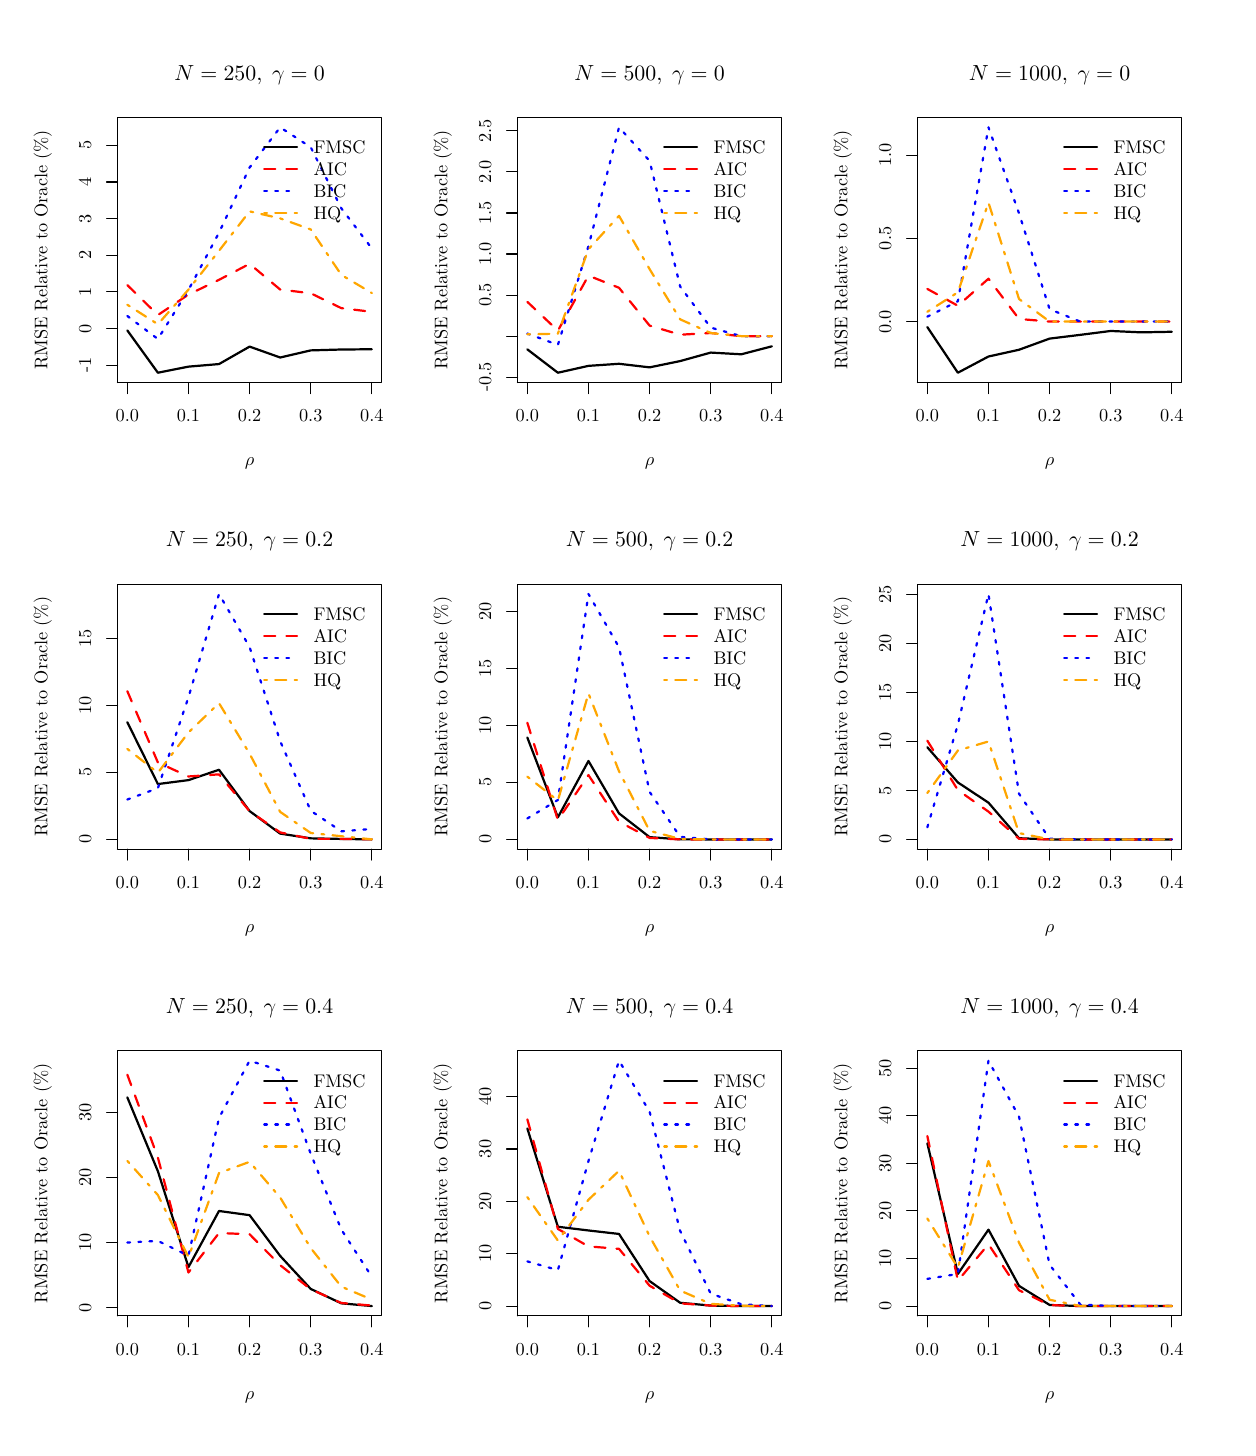
\begin{tikzpicture}[x=1pt,y=1pt]
\definecolor[named]{fillColor}{rgb}{1.00,1.00,1.00}
\path[use as bounding box,fill=fillColor,fill opacity=0.00] (0,0) rectangle (433.62,505.89);
\begin{scope}
\path[clip] ( 32.47,377.65) rectangle (127.91,473.42);
\definecolor[named]{drawColor}{rgb}{0.00,0.00,0.00}

\path[draw=drawColor,line width= 0.8pt,line join=round,line cap=round] ( 36.01,396.49) --
	( 47.05,381.20) --
	( 58.10,383.40) --
	( 69.14,384.33) --
	( 80.19,390.64) --
	( 91.24,386.70) --
	(102.28,389.27) --
	(113.33,389.59) --
	(124.37,389.68);
\end{scope}
\begin{scope}
\path[clip] (  0.00,  0.00) rectangle (433.62,505.89);
\definecolor[named]{drawColor}{rgb}{0.00,0.00,0.00}

\path[draw=drawColor,line width= 0.4pt,line join=round,line cap=round] ( 36.01,377.65) -- (124.37,377.65);

\path[draw=drawColor,line width= 0.4pt,line join=round,line cap=round] ( 36.01,377.65) -- ( 36.01,373.69);

\path[draw=drawColor,line width= 0.4pt,line join=round,line cap=round] ( 58.10,377.65) -- ( 58.10,373.69);

\path[draw=drawColor,line width= 0.4pt,line join=round,line cap=round] ( 80.19,377.65) -- ( 80.19,373.69);

\path[draw=drawColor,line width= 0.4pt,line join=round,line cap=round] (102.28,377.65) -- (102.28,373.69);

\path[draw=drawColor,line width= 0.4pt,line join=round,line cap=round] (124.37,377.65) -- (124.37,373.69);

\node[text=drawColor,anchor=base,inner sep=0pt, outer sep=0pt, scale=  0.66] at ( 36.01,363.40) {0.0};

\node[text=drawColor,anchor=base,inner sep=0pt, outer sep=0pt, scale=  0.66] at ( 58.10,363.40) {0.1};

\node[text=drawColor,anchor=base,inner sep=0pt, outer sep=0pt, scale=  0.66] at ( 80.19,363.40) {0.2};

\node[text=drawColor,anchor=base,inner sep=0pt, outer sep=0pt, scale=  0.66] at (102.28,363.40) {0.3};

\node[text=drawColor,anchor=base,inner sep=0pt, outer sep=0pt, scale=  0.66] at (124.37,363.40) {0.4};

\path[draw=drawColor,line width= 0.4pt,line join=round,line cap=round] ( 32.47,383.95) -- ( 32.47,463.36);

\path[draw=drawColor,line width= 0.4pt,line join=round,line cap=round] ( 32.47,383.95) -- ( 28.51,383.95);

\path[draw=drawColor,line width= 0.4pt,line join=round,line cap=round] ( 32.47,397.19) -- ( 28.51,397.19);

\path[draw=drawColor,line width= 0.4pt,line join=round,line cap=round] ( 32.47,410.42) -- ( 28.51,410.42);

\path[draw=drawColor,line width= 0.4pt,line join=round,line cap=round] ( 32.47,423.66) -- ( 28.51,423.66);

\path[draw=drawColor,line width= 0.4pt,line join=round,line cap=round] ( 32.47,436.89) -- ( 28.51,436.89);

\path[draw=drawColor,line width= 0.4pt,line join=round,line cap=round] ( 32.47,450.12) -- ( 28.51,450.12);

\path[draw=drawColor,line width= 0.4pt,line join=round,line cap=round] ( 32.47,463.36) -- ( 28.51,463.36);

\node[text=drawColor,rotate= 90.00,anchor=base,inner sep=0pt, outer sep=0pt, scale=  0.66] at ( 22.97,383.95) {-1};

\node[text=drawColor,rotate= 90.00,anchor=base,inner sep=0pt, outer sep=0pt, scale=  0.66] at ( 22.97,397.19) {0};

\node[text=drawColor,rotate= 90.00,anchor=base,inner sep=0pt, outer sep=0pt, scale=  0.66] at ( 22.97,410.42) {1};

\node[text=drawColor,rotate= 90.00,anchor=base,inner sep=0pt, outer sep=0pt, scale=  0.66] at ( 22.97,423.66) {2};

\node[text=drawColor,rotate= 90.00,anchor=base,inner sep=0pt, outer sep=0pt, scale=  0.66] at ( 22.97,436.89) {3};

\node[text=drawColor,rotate= 90.00,anchor=base,inner sep=0pt, outer sep=0pt, scale=  0.66] at ( 22.97,450.12) {4};

\node[text=drawColor,rotate= 90.00,anchor=base,inner sep=0pt, outer sep=0pt, scale=  0.66] at ( 22.97,463.36) {5};

\path[draw=drawColor,line width= 0.4pt,line join=round,line cap=round] ( 32.47,377.65) --
	(127.91,377.65) --
	(127.91,473.42) --
	( 32.47,473.42) --
	( 32.47,377.65);
\end{scope}
\begin{scope}
\path[clip] (  0.00,337.26) rectangle (144.54,505.89);
\definecolor[named]{drawColor}{rgb}{0.00,0.00,0.00}

\node[text=drawColor,anchor=base,inner sep=0pt, outer sep=0pt, scale=  0.79] at ( 80.19,486.92) {\bfseries $N=250, \;\gamma=0$};

\node[text=drawColor,anchor=base,inner sep=0pt, outer sep=0pt, scale=  0.66] at ( 80.19,347.56) {$\rho$};

\node[text=drawColor,rotate= 90.00,anchor=base,inner sep=0pt, outer sep=0pt, scale=  0.66] at (  7.13,425.53) {RMSE Relative to Oracle (\%)};
\end{scope}
\begin{scope}
\path[clip] ( 32.47,377.65) rectangle (127.91,473.42);
\definecolor[named]{drawColor}{rgb}{1.00,0.00,0.00}

\path[draw=drawColor,line width= 0.8pt,dash pattern=on 4pt off 4pt ,line join=round,line cap=round] ( 36.01,412.87) --
	( 47.05,402.05) --
	( 58.10,409.44) --
	( 69.14,414.77) --
	( 80.19,420.55) --
	( 91.24,411.26) --
	(102.28,409.91) --
	(113.33,404.54) --
	(124.37,403.21);
\definecolor[named]{drawColor}{rgb}{0.00,0.00,1.00}

\path[draw=drawColor,line width= 0.8pt,dash pattern=on 1pt off 3pt ,line join=round,line cap=round] ( 36.01,401.70) --
	( 47.05,393.38) --
	( 58.10,411.10) --
	( 69.14,431.79) --
	( 80.19,455.35) --
	( 91.24,469.87) --
	(102.28,462.69) --
	(113.33,440.62) --
	(124.37,426.10);
\definecolor[named]{drawColor}{rgb}{1.00,0.65,0.00}

\path[draw=drawColor,line width= 0.8pt,dash pattern=on 1pt off 3pt on 4pt off 3pt ,line join=round,line cap=round] ( 36.01,405.76) --
	( 47.05,398.72) --
	( 58.10,411.22) --
	( 69.14,425.26) --
	( 80.19,439.51) --
	( 91.24,436.97) --
	(102.28,432.98) --
	(113.33,416.56) --
	(124.37,409.99);
\definecolor[named]{drawColor}{rgb}{0.00,0.00,0.00}

\path[draw=drawColor,line width= 0.8pt,line join=round,line cap=round] ( 85.47,462.63) -- ( 97.35,462.63);
\definecolor[named]{drawColor}{rgb}{1.00,0.00,0.00}

\path[draw=drawColor,line width= 0.8pt,dash pattern=on 4pt off 4pt ,line join=round,line cap=round] ( 85.47,454.71) -- ( 97.35,454.71);
\definecolor[named]{drawColor}{rgb}{0.00,0.00,1.00}

\path[draw=drawColor,line width= 0.8pt,dash pattern=on 1pt off 3pt ,line join=round,line cap=round] ( 85.47,446.79) -- ( 97.35,446.79);
\definecolor[named]{drawColor}{rgb}{1.00,0.65,0.00}

\path[draw=drawColor,line width= 0.8pt,dash pattern=on 1pt off 3pt on 4pt off 3pt ,line join=round,line cap=round] ( 85.47,438.87) -- ( 97.35,438.87);
\definecolor[named]{drawColor}{rgb}{0.00,0.00,0.00}

\node[text=drawColor,anchor=base west,inner sep=0pt, outer sep=0pt, scale=  0.66] at (103.29,460.35) {FMSC};

\node[text=drawColor,anchor=base west,inner sep=0pt, outer sep=0pt, scale=  0.66] at (103.29,452.43) {AIC};

\node[text=drawColor,anchor=base west,inner sep=0pt, outer sep=0pt, scale=  0.66] at (103.29,444.51) {BIC};

\node[text=drawColor,anchor=base west,inner sep=0pt, outer sep=0pt, scale=  0.66] at (103.29,436.59) {HQ};
\end{scope}
\begin{scope}
\path[clip] (177.01,377.65) rectangle (272.45,473.42);
\definecolor[named]{drawColor}{rgb}{0.00,0.00,0.00}

\path[draw=drawColor,line width= 0.8pt,line join=round,line cap=round] (180.55,389.64) --
	(191.59,381.20) --
	(202.64,383.68) --
	(213.68,384.43) --
	(224.73,383.14) --
	(235.78,385.41) --
	(246.82,388.48) --
	(257.87,387.86) --
	(268.91,390.74);
\end{scope}
\begin{scope}
\path[clip] (  0.00,  0.00) rectangle (433.62,505.89);
\definecolor[named]{drawColor}{rgb}{0.00,0.00,0.00}

\path[draw=drawColor,line width= 0.4pt,line join=round,line cap=round] (180.55,377.65) -- (268.91,377.65);

\path[draw=drawColor,line width= 0.4pt,line join=round,line cap=round] (180.55,377.65) -- (180.55,373.69);

\path[draw=drawColor,line width= 0.4pt,line join=round,line cap=round] (202.64,377.65) -- (202.64,373.69);

\path[draw=drawColor,line width= 0.4pt,line join=round,line cap=round] (224.73,377.65) -- (224.73,373.69);

\path[draw=drawColor,line width= 0.4pt,line join=round,line cap=round] (246.82,377.65) -- (246.82,373.69);

\path[draw=drawColor,line width= 0.4pt,line join=round,line cap=round] (268.91,377.65) -- (268.91,373.69);

\node[text=drawColor,anchor=base,inner sep=0pt, outer sep=0pt, scale=  0.66] at (180.55,363.40) {0.0};

\node[text=drawColor,anchor=base,inner sep=0pt, outer sep=0pt, scale=  0.66] at (202.64,363.40) {0.1};

\node[text=drawColor,anchor=base,inner sep=0pt, outer sep=0pt, scale=  0.66] at (224.73,363.40) {0.2};

\node[text=drawColor,anchor=base,inner sep=0pt, outer sep=0pt, scale=  0.66] at (246.82,363.40) {0.3};

\node[text=drawColor,anchor=base,inner sep=0pt, outer sep=0pt, scale=  0.66] at (268.91,363.40) {0.4};

\path[draw=drawColor,line width= 0.4pt,line join=round,line cap=round] (177.01,379.57) -- (177.01,468.61);

\path[draw=drawColor,line width= 0.4pt,line join=round,line cap=round] (177.01,379.57) -- (173.05,379.57);

\path[draw=drawColor,line width= 0.4pt,line join=round,line cap=round] (177.01,394.41) -- (173.05,394.41);

\path[draw=drawColor,line width= 0.4pt,line join=round,line cap=round] (177.01,409.25) -- (173.05,409.25);

\path[draw=drawColor,line width= 0.4pt,line join=round,line cap=round] (177.01,424.09) -- (173.05,424.09);

\path[draw=drawColor,line width= 0.4pt,line join=round,line cap=round] (177.01,438.93) -- (173.05,438.93);

\path[draw=drawColor,line width= 0.4pt,line join=round,line cap=round] (177.01,453.77) -- (173.05,453.77);

\path[draw=drawColor,line width= 0.4pt,line join=round,line cap=round] (177.01,468.61) -- (173.05,468.61);

\node[text=drawColor,rotate= 90.00,anchor=base,inner sep=0pt, outer sep=0pt, scale=  0.66] at (167.51,379.57) {-0.5};

\node[text=drawColor,rotate= 90.00,anchor=base,inner sep=0pt, outer sep=0pt, scale=  0.66] at (167.51,409.25) {0.5};

\node[text=drawColor,rotate= 90.00,anchor=base,inner sep=0pt, outer sep=0pt, scale=  0.66] at (167.51,424.09) {1.0};

\node[text=drawColor,rotate= 90.00,anchor=base,inner sep=0pt, outer sep=0pt, scale=  0.66] at (167.51,438.93) {1.5};

\node[text=drawColor,rotate= 90.00,anchor=base,inner sep=0pt, outer sep=0pt, scale=  0.66] at (167.51,453.77) {2.0};

\node[text=drawColor,rotate= 90.00,anchor=base,inner sep=0pt, outer sep=0pt, scale=  0.66] at (167.51,468.61) {2.5};

\path[draw=drawColor,line width= 0.4pt,line join=round,line cap=round] (177.01,377.65) --
	(272.45,377.65) --
	(272.45,473.42) --
	(177.01,473.42) --
	(177.01,377.65);
\end{scope}
\begin{scope}
\path[clip] (144.54,337.26) rectangle (289.08,505.89);
\definecolor[named]{drawColor}{rgb}{0.00,0.00,0.00}

\node[text=drawColor,anchor=base,inner sep=0pt, outer sep=0pt, scale=  0.79] at (224.73,486.92) {\bfseries $N=500, \;\gamma=0$};

\node[text=drawColor,anchor=base,inner sep=0pt, outer sep=0pt, scale=  0.66] at (224.73,347.56) {$\rho$};

\node[text=drawColor,rotate= 90.00,anchor=base,inner sep=0pt, outer sep=0pt, scale=  0.66] at (151.67,425.53) {RMSE Relative to Oracle (\%)};
\end{scope}
\begin{scope}
\path[clip] (177.01,377.65) rectangle (272.45,473.42);
\definecolor[named]{drawColor}{rgb}{1.00,0.00,0.00}

\path[draw=drawColor,line width= 0.8pt,dash pattern=on 4pt off 4pt ,line join=round,line cap=round] (180.55,406.81) --
	(191.59,396.39) --
	(202.64,416.29) --
	(213.68,411.89) --
	(224.73,398.23) --
	(235.78,394.94) --
	(246.82,395.55) --
	(257.87,394.41) --
	(268.91,394.41);
\definecolor[named]{drawColor}{rgb}{0.00,0.00,1.00}

\path[draw=drawColor,line width= 0.8pt,dash pattern=on 1pt off 3pt ,line join=round,line cap=round] (180.55,395.37) --
	(191.59,391.25) --
	(202.64,426.93) --
	(213.68,469.87) --
	(224.73,457.75) --
	(235.78,412.35) --
	(246.82,397.50) --
	(257.87,394.41) --
	(268.91,394.41);
\definecolor[named]{drawColor}{rgb}{1.00,0.65,0.00}

\path[draw=drawColor,line width= 0.8pt,dash pattern=on 1pt off 3pt on 4pt off 3pt ,line join=round,line cap=round] (180.55,395.07) --
	(191.59,395.31) --
	(202.64,425.84) --
	(213.68,437.89) --
	(224.73,418.64) --
	(235.78,400.49) --
	(246.82,395.55) --
	(257.87,394.41) --
	(268.91,394.41);
\definecolor[named]{drawColor}{rgb}{0.00,0.00,0.00}

\path[draw=drawColor,line width= 0.8pt,line join=round,line cap=round] (230.01,462.63) -- (241.89,462.63);
\definecolor[named]{drawColor}{rgb}{1.00,0.00,0.00}

\path[draw=drawColor,line width= 0.8pt,dash pattern=on 4pt off 4pt ,line join=round,line cap=round] (230.01,454.71) -- (241.89,454.71);
\definecolor[named]{drawColor}{rgb}{0.00,0.00,1.00}

\path[draw=drawColor,line width= 0.8pt,dash pattern=on 1pt off 3pt ,line join=round,line cap=round] (230.01,446.79) -- (241.89,446.79);
\definecolor[named]{drawColor}{rgb}{1.00,0.65,0.00}

\path[draw=drawColor,line width= 0.8pt,dash pattern=on 1pt off 3pt on 4pt off 3pt ,line join=round,line cap=round] (230.01,438.87) -- (241.89,438.87);
\definecolor[named]{drawColor}{rgb}{0.00,0.00,0.00}

\node[text=drawColor,anchor=base west,inner sep=0pt, outer sep=0pt, scale=  0.66] at (247.83,460.35) {FMSC};

\node[text=drawColor,anchor=base west,inner sep=0pt, outer sep=0pt, scale=  0.66] at (247.83,452.43) {AIC};

\node[text=drawColor,anchor=base west,inner sep=0pt, outer sep=0pt, scale=  0.66] at (247.83,444.51) {BIC};

\node[text=drawColor,anchor=base west,inner sep=0pt, outer sep=0pt, scale=  0.66] at (247.83,436.59) {HQ};
\end{scope}
\begin{scope}
\path[clip] (321.55,377.65) rectangle (416.99,473.42);
\definecolor[named]{drawColor}{rgb}{0.00,0.00,0.00}

\path[draw=drawColor,line width= 0.8pt,line join=round,line cap=round] (325.09,397.69) --
	(336.13,381.20) --
	(347.18,387.06) --
	(358.22,389.50) --
	(369.27,393.53) --
	(380.32,394.88) --
	(391.36,396.29) --
	(402.41,395.79) --
	(413.45,396.00);
\end{scope}
\begin{scope}
\path[clip] (  0.00,  0.00) rectangle (433.62,505.89);
\definecolor[named]{drawColor}{rgb}{0.00,0.00,0.00}

\path[draw=drawColor,line width= 0.4pt,line join=round,line cap=round] (325.09,377.65) -- (413.45,377.65);

\path[draw=drawColor,line width= 0.4pt,line join=round,line cap=round] (325.09,377.65) -- (325.09,373.69);

\path[draw=drawColor,line width= 0.4pt,line join=round,line cap=round] (347.18,377.65) -- (347.18,373.69);

\path[draw=drawColor,line width= 0.4pt,line join=round,line cap=round] (369.27,377.65) -- (369.27,373.69);

\path[draw=drawColor,line width= 0.4pt,line join=round,line cap=round] (391.36,377.65) -- (391.36,373.69);

\path[draw=drawColor,line width= 0.4pt,line join=round,line cap=round] (413.45,377.65) -- (413.45,373.69);

\node[text=drawColor,anchor=base,inner sep=0pt, outer sep=0pt, scale=  0.66] at (325.09,363.40) {0.0};

\node[text=drawColor,anchor=base,inner sep=0pt, outer sep=0pt, scale=  0.66] at (347.18,363.40) {0.1};

\node[text=drawColor,anchor=base,inner sep=0pt, outer sep=0pt, scale=  0.66] at (369.27,363.40) {0.2};

\node[text=drawColor,anchor=base,inner sep=0pt, outer sep=0pt, scale=  0.66] at (391.36,363.40) {0.3};

\node[text=drawColor,anchor=base,inner sep=0pt, outer sep=0pt, scale=  0.66] at (413.45,363.40) {0.4};

\path[draw=drawColor,line width= 0.4pt,line join=round,line cap=round] (321.55,399.69) -- (321.55,459.81);

\path[draw=drawColor,line width= 0.4pt,line join=round,line cap=round] (321.55,399.69) -- (317.59,399.69);

\path[draw=drawColor,line width= 0.4pt,line join=round,line cap=round] (321.55,429.75) -- (317.59,429.75);

\path[draw=drawColor,line width= 0.4pt,line join=round,line cap=round] (321.55,459.81) -- (317.59,459.81);

\node[text=drawColor,rotate= 90.00,anchor=base,inner sep=0pt, outer sep=0pt, scale=  0.66] at (312.05,399.69) {0.0};

\node[text=drawColor,rotate= 90.00,anchor=base,inner sep=0pt, outer sep=0pt, scale=  0.66] at (312.05,429.75) {0.5};

\node[text=drawColor,rotate= 90.00,anchor=base,inner sep=0pt, outer sep=0pt, scale=  0.66] at (312.05,459.81) {1.0};

\path[draw=drawColor,line width= 0.4pt,line join=round,line cap=round] (321.55,377.65) --
	(416.99,377.65) --
	(416.99,473.42) --
	(321.55,473.42) --
	(321.55,377.65);
\end{scope}
\begin{scope}
\path[clip] (289.08,337.26) rectangle (433.62,505.89);
\definecolor[named]{drawColor}{rgb}{0.00,0.00,0.00}

\node[text=drawColor,anchor=base,inner sep=0pt, outer sep=0pt, scale=  0.79] at (369.27,486.92) {\bfseries $N=1000, \;\gamma=0$};

\node[text=drawColor,anchor=base,inner sep=0pt, outer sep=0pt, scale=  0.66] at (369.27,347.56) {$\rho$};

\node[text=drawColor,rotate= 90.00,anchor=base,inner sep=0pt, outer sep=0pt, scale=  0.66] at (296.21,425.53) {RMSE Relative to Oracle (\%)};
\end{scope}
\begin{scope}
\path[clip] (321.55,377.65) rectangle (416.99,473.42);
\definecolor[named]{drawColor}{rgb}{1.00,0.00,0.00}

\path[draw=drawColor,line width= 0.8pt,dash pattern=on 4pt off 4pt ,line join=round,line cap=round] (325.09,411.48) --
	(336.13,405.40) --
	(347.18,415.17) --
	(358.22,400.63) --
	(369.27,399.69) --
	(380.32,399.69) --
	(391.36,399.69) --
	(402.41,399.69) --
	(413.45,399.69);
\definecolor[named]{drawColor}{rgb}{0.00,0.00,1.00}

\path[draw=drawColor,line width= 0.8pt,dash pattern=on 1pt off 3pt ,line join=round,line cap=round] (325.09,401.45) --
	(336.13,407.03) --
	(347.18,469.87) --
	(358.22,438.81) --
	(369.27,404.16) --
	(380.32,399.69) --
	(391.36,399.69) --
	(402.41,399.69) --
	(413.45,399.69);
\definecolor[named]{drawColor}{rgb}{1.00,0.65,0.00}

\path[draw=drawColor,line width= 0.8pt,dash pattern=on 1pt off 3pt on 4pt off 3pt ,line join=round,line cap=round] (325.09,403.22) --
	(336.13,410.25) --
	(347.18,442.68) --
	(358.22,407.84) --
	(369.27,399.69) --
	(380.32,399.69) --
	(391.36,399.69) --
	(402.41,399.69) --
	(413.45,399.69);
\definecolor[named]{drawColor}{rgb}{0.00,0.00,0.00}

\path[draw=drawColor,line width= 0.8pt,line join=round,line cap=round] (374.55,462.63) -- (386.43,462.63);
\definecolor[named]{drawColor}{rgb}{1.00,0.00,0.00}

\path[draw=drawColor,line width= 0.8pt,dash pattern=on 4pt off 4pt ,line join=round,line cap=round] (374.55,454.71) -- (386.43,454.71);
\definecolor[named]{drawColor}{rgb}{0.00,0.00,1.00}

\path[draw=drawColor,line width= 0.8pt,dash pattern=on 1pt off 3pt ,line join=round,line cap=round] (374.55,446.79) -- (386.43,446.79);
\definecolor[named]{drawColor}{rgb}{1.00,0.65,0.00}

\path[draw=drawColor,line width= 0.8pt,dash pattern=on 1pt off 3pt on 4pt off 3pt ,line join=round,line cap=round] (374.55,438.87) -- (386.43,438.87);
\definecolor[named]{drawColor}{rgb}{0.00,0.00,0.00}

\node[text=drawColor,anchor=base west,inner sep=0pt, outer sep=0pt, scale=  0.66] at (392.37,460.35) {FMSC};

\node[text=drawColor,anchor=base west,inner sep=0pt, outer sep=0pt, scale=  0.66] at (392.37,452.43) {AIC};

\node[text=drawColor,anchor=base west,inner sep=0pt, outer sep=0pt, scale=  0.66] at (392.37,444.51) {BIC};

\node[text=drawColor,anchor=base west,inner sep=0pt, outer sep=0pt, scale=  0.66] at (392.37,436.59) {HQ};
\end{scope}
\begin{scope}
\path[clip] ( 32.47,209.02) rectangle (127.91,304.79);
\definecolor[named]{drawColor}{rgb}{0.00,0.00,0.00}

\path[draw=drawColor,line width= 0.8pt,line join=round,line cap=round] ( 36.01,254.91) --
	( 47.05,232.57) --
	( 58.10,233.99) --
	( 69.14,237.73) --
	( 80.19,222.81) --
	( 91.24,214.66) --
	(102.28,212.95) --
	(113.33,212.74) --
	(124.37,212.57);
\end{scope}
\begin{scope}
\path[clip] (  0.00,  0.00) rectangle (433.62,505.89);
\definecolor[named]{drawColor}{rgb}{0.00,0.00,0.00}

\path[draw=drawColor,line width= 0.4pt,line join=round,line cap=round] ( 36.01,209.02) -- (124.37,209.02);

\path[draw=drawColor,line width= 0.4pt,line join=round,line cap=round] ( 36.01,209.02) -- ( 36.01,205.06);

\path[draw=drawColor,line width= 0.4pt,line join=round,line cap=round] ( 58.10,209.02) -- ( 58.10,205.06);

\path[draw=drawColor,line width= 0.4pt,line join=round,line cap=round] ( 80.19,209.02) -- ( 80.19,205.06);

\path[draw=drawColor,line width= 0.4pt,line join=round,line cap=round] (102.28,209.02) -- (102.28,205.06);

\path[draw=drawColor,line width= 0.4pt,line join=round,line cap=round] (124.37,209.02) -- (124.37,205.06);

\node[text=drawColor,anchor=base,inner sep=0pt, outer sep=0pt, scale=  0.66] at ( 36.01,194.77) {0.0};

\node[text=drawColor,anchor=base,inner sep=0pt, outer sep=0pt, scale=  0.66] at ( 58.10,194.77) {0.1};

\node[text=drawColor,anchor=base,inner sep=0pt, outer sep=0pt, scale=  0.66] at ( 80.19,194.77) {0.2};

\node[text=drawColor,anchor=base,inner sep=0pt, outer sep=0pt, scale=  0.66] at (102.28,194.77) {0.3};

\node[text=drawColor,anchor=base,inner sep=0pt, outer sep=0pt, scale=  0.66] at (124.37,194.77) {0.4};

\path[draw=drawColor,line width= 0.4pt,line join=round,line cap=round] ( 32.47,212.59) -- ( 32.47,285.16);

\path[draw=drawColor,line width= 0.4pt,line join=round,line cap=round] ( 32.47,212.59) -- ( 28.51,212.59);

\path[draw=drawColor,line width= 0.4pt,line join=round,line cap=round] ( 32.47,236.78) -- ( 28.51,236.78);

\path[draw=drawColor,line width= 0.4pt,line join=round,line cap=round] ( 32.47,260.97) -- ( 28.51,260.97);

\path[draw=drawColor,line width= 0.4pt,line join=round,line cap=round] ( 32.47,285.16) -- ( 28.51,285.16);

\node[text=drawColor,rotate= 90.00,anchor=base,inner sep=0pt, outer sep=0pt, scale=  0.66] at ( 22.97,212.59) {0};

\node[text=drawColor,rotate= 90.00,anchor=base,inner sep=0pt, outer sep=0pt, scale=  0.66] at ( 22.97,236.78) {5};

\node[text=drawColor,rotate= 90.00,anchor=base,inner sep=0pt, outer sep=0pt, scale=  0.66] at ( 22.97,260.97) {10};

\node[text=drawColor,rotate= 90.00,anchor=base,inner sep=0pt, outer sep=0pt, scale=  0.66] at ( 22.97,285.16) {15};

\path[draw=drawColor,line width= 0.4pt,line join=round,line cap=round] ( 32.47,209.02) --
	(127.91,209.02) --
	(127.91,304.79) --
	( 32.47,304.79) --
	( 32.47,209.02);
\end{scope}
\begin{scope}
\path[clip] (  0.00,168.63) rectangle (144.54,337.26);
\definecolor[named]{drawColor}{rgb}{0.00,0.00,0.00}

\node[text=drawColor,anchor=base,inner sep=0pt, outer sep=0pt, scale=  0.79] at ( 80.19,318.29) {\bfseries $N=250, \;\gamma=0.2$};

\node[text=drawColor,anchor=base,inner sep=0pt, outer sep=0pt, scale=  0.66] at ( 80.19,178.93) {$\rho$};

\node[text=drawColor,rotate= 90.00,anchor=base,inner sep=0pt, outer sep=0pt, scale=  0.66] at (  7.13,256.90) {RMSE Relative to Oracle (\%)};
\end{scope}
\begin{scope}
\path[clip] ( 32.47,209.02) rectangle (127.91,304.79);
\definecolor[named]{drawColor}{rgb}{1.00,0.00,0.00}

\path[draw=drawColor,line width= 0.8pt,dash pattern=on 4pt off 4pt ,line join=round,line cap=round] ( 36.01,266.12) --
	( 47.05,240.36) --
	( 58.10,235.31) --
	( 69.14,236.07) --
	( 80.19,222.76) --
	( 91.24,215.10) --
	(102.28,212.76) --
	(113.33,212.76) --
	(124.37,212.59);
\definecolor[named]{drawColor}{rgb}{0.00,0.00,1.00}

\path[draw=drawColor,line width= 0.8pt,dash pattern=on 1pt off 3pt ,line join=round,line cap=round] ( 36.01,226.98) --
	( 47.05,231.09) --
	( 58.10,263.94) --
	( 69.14,301.24) --
	( 80.19,282.08) --
	( 91.24,248.07) --
	(102.28,222.93) --
	(113.33,215.49) --
	(124.37,216.35);
\definecolor[named]{drawColor}{rgb}{1.00,0.65,0.00}

\path[draw=drawColor,line width= 0.8pt,dash pattern=on 1pt off 3pt on 4pt off 3pt ,line join=round,line cap=round] ( 36.01,245.26) --
	( 47.05,236.64) --
	( 58.10,251.20) --
	( 69.14,261.81) --
	( 80.19,243.54) --
	( 91.24,222.52) --
	(102.28,214.89) --
	(113.33,213.72) --
	(124.37,212.59);
\definecolor[named]{drawColor}{rgb}{0.00,0.00,0.00}

\path[draw=drawColor,line width= 0.8pt,line join=round,line cap=round] ( 85.47,294.00) -- ( 97.35,294.00);
\definecolor[named]{drawColor}{rgb}{1.00,0.00,0.00}

\path[draw=drawColor,line width= 0.8pt,dash pattern=on 4pt off 4pt ,line join=round,line cap=round] ( 85.47,286.08) -- ( 97.35,286.08);
\definecolor[named]{drawColor}{rgb}{0.00,0.00,1.00}

\path[draw=drawColor,line width= 0.8pt,dash pattern=on 1pt off 3pt ,line join=round,line cap=round] ( 85.47,278.16) -- ( 97.35,278.16);
\definecolor[named]{drawColor}{rgb}{1.00,0.65,0.00}

\path[draw=drawColor,line width= 0.8pt,dash pattern=on 1pt off 3pt on 4pt off 3pt ,line join=round,line cap=round] ( 85.47,270.24) -- ( 97.35,270.24);
\definecolor[named]{drawColor}{rgb}{0.00,0.00,0.00}

\node[text=drawColor,anchor=base west,inner sep=0pt, outer sep=0pt, scale=  0.66] at (103.29,291.72) {FMSC};

\node[text=drawColor,anchor=base west,inner sep=0pt, outer sep=0pt, scale=  0.66] at (103.29,283.80) {AIC};

\node[text=drawColor,anchor=base west,inner sep=0pt, outer sep=0pt, scale=  0.66] at (103.29,275.88) {BIC};

\node[text=drawColor,anchor=base west,inner sep=0pt, outer sep=0pt, scale=  0.66] at (103.29,267.96) {HQ};
\end{scope}
\begin{scope}
\path[clip] (177.01,209.02) rectangle (272.45,304.79);
\definecolor[named]{drawColor}{rgb}{0.00,0.00,0.00}

\path[draw=drawColor,line width= 0.8pt,line join=round,line cap=round] (180.55,249.38) --
	(191.59,220.54) --
	(202.64,240.91) --
	(213.68,221.97) --
	(224.73,213.39) --
	(235.78,212.58) --
	(246.82,212.57) --
	(257.87,212.57) --
	(268.91,212.57);
\end{scope}
\begin{scope}
\path[clip] (  0.00,  0.00) rectangle (433.62,505.89);
\definecolor[named]{drawColor}{rgb}{0.00,0.00,0.00}

\path[draw=drawColor,line width= 0.4pt,line join=round,line cap=round] (180.55,209.02) -- (268.91,209.02);

\path[draw=drawColor,line width= 0.4pt,line join=round,line cap=round] (180.55,209.02) -- (180.55,205.06);

\path[draw=drawColor,line width= 0.4pt,line join=round,line cap=round] (202.64,209.02) -- (202.64,205.06);

\path[draw=drawColor,line width= 0.4pt,line join=round,line cap=round] (224.73,209.02) -- (224.73,205.06);

\path[draw=drawColor,line width= 0.4pt,line join=round,line cap=round] (246.82,209.02) -- (246.82,205.06);

\path[draw=drawColor,line width= 0.4pt,line join=round,line cap=round] (268.91,209.02) -- (268.91,205.06);

\node[text=drawColor,anchor=base,inner sep=0pt, outer sep=0pt, scale=  0.66] at (180.55,194.77) {0.0};

\node[text=drawColor,anchor=base,inner sep=0pt, outer sep=0pt, scale=  0.66] at (202.64,194.77) {0.1};

\node[text=drawColor,anchor=base,inner sep=0pt, outer sep=0pt, scale=  0.66] at (224.73,194.77) {0.2};

\node[text=drawColor,anchor=base,inner sep=0pt, outer sep=0pt, scale=  0.66] at (246.82,194.77) {0.3};

\node[text=drawColor,anchor=base,inner sep=0pt, outer sep=0pt, scale=  0.66] at (268.91,194.77) {0.4};

\path[draw=drawColor,line width= 0.4pt,line join=round,line cap=round] (177.01,212.57) -- (177.01,295.01);

\path[draw=drawColor,line width= 0.4pt,line join=round,line cap=round] (177.01,212.57) -- (173.05,212.57);

\path[draw=drawColor,line width= 0.4pt,line join=round,line cap=round] (177.01,233.18) -- (173.05,233.18);

\path[draw=drawColor,line width= 0.4pt,line join=round,line cap=round] (177.01,253.79) -- (173.05,253.79);

\path[draw=drawColor,line width= 0.4pt,line join=round,line cap=round] (177.01,274.40) -- (173.05,274.40);

\path[draw=drawColor,line width= 0.4pt,line join=round,line cap=round] (177.01,295.01) -- (173.05,295.01);

\node[text=drawColor,rotate= 90.00,anchor=base,inner sep=0pt, outer sep=0pt, scale=  0.66] at (167.51,212.57) {0};

\node[text=drawColor,rotate= 90.00,anchor=base,inner sep=0pt, outer sep=0pt, scale=  0.66] at (167.51,233.18) {5};

\node[text=drawColor,rotate= 90.00,anchor=base,inner sep=0pt, outer sep=0pt, scale=  0.66] at (167.51,253.79) {10};

\node[text=drawColor,rotate= 90.00,anchor=base,inner sep=0pt, outer sep=0pt, scale=  0.66] at (167.51,274.40) {15};

\node[text=drawColor,rotate= 90.00,anchor=base,inner sep=0pt, outer sep=0pt, scale=  0.66] at (167.51,295.01) {20};

\path[draw=drawColor,line width= 0.4pt,line join=round,line cap=round] (177.01,209.02) --
	(272.45,209.02) --
	(272.45,304.79) --
	(177.01,304.79) --
	(177.01,209.02);
\end{scope}
\begin{scope}
\path[clip] (144.54,168.63) rectangle (289.08,337.26);
\definecolor[named]{drawColor}{rgb}{0.00,0.00,0.00}

\node[text=drawColor,anchor=base,inner sep=0pt, outer sep=0pt, scale=  0.79] at (224.73,318.29) {\bfseries $N=500, \;\gamma=0.2$};

\node[text=drawColor,anchor=base,inner sep=0pt, outer sep=0pt, scale=  0.66] at (224.73,178.93) {$\rho$};

\node[text=drawColor,rotate= 90.00,anchor=base,inner sep=0pt, outer sep=0pt, scale=  0.66] at (151.67,256.90) {RMSE Relative to Oracle (\%)};
\end{scope}
\begin{scope}
\path[clip] (177.01,209.02) rectangle (272.45,304.79);
\definecolor[named]{drawColor}{rgb}{1.00,0.00,0.00}

\path[draw=drawColor,line width= 0.8pt,dash pattern=on 4pt off 4pt ,line join=round,line cap=round] (180.55,254.72) --
	(191.59,219.59) --
	(202.64,235.82) --
	(213.68,218.97) --
	(224.73,213.10) --
	(235.78,212.57) --
	(246.82,212.57) --
	(257.87,212.57) --
	(268.91,212.57);
\definecolor[named]{drawColor}{rgb}{0.00,0.00,1.00}

\path[draw=drawColor,line width= 0.8pt,dash pattern=on 1pt off 3pt ,line join=round,line cap=round] (180.55,220.13) --
	(191.59,226.82) --
	(202.64,301.24) --
	(213.68,282.01) --
	(224.73,229.74) --
	(235.78,213.49) --
	(246.82,212.57) --
	(257.87,212.57) --
	(268.91,212.57);
\definecolor[named]{drawColor}{rgb}{1.00,0.65,0.00}

\path[draw=drawColor,line width= 0.8pt,dash pattern=on 1pt off 3pt on 4pt off 3pt ,line join=round,line cap=round] (180.55,235.25) --
	(191.59,226.61) --
	(202.64,265.34) --
	(213.68,237.18) --
	(224.73,215.66) --
	(235.78,212.74) --
	(246.82,212.57) --
	(257.87,212.57) --
	(268.91,212.57);
\definecolor[named]{drawColor}{rgb}{0.00,0.00,0.00}

\path[draw=drawColor,line width= 0.8pt,line join=round,line cap=round] (230.01,294.00) -- (241.89,294.00);
\definecolor[named]{drawColor}{rgb}{1.00,0.00,0.00}

\path[draw=drawColor,line width= 0.8pt,dash pattern=on 4pt off 4pt ,line join=round,line cap=round] (230.01,286.08) -- (241.89,286.08);
\definecolor[named]{drawColor}{rgb}{0.00,0.00,1.00}

\path[draw=drawColor,line width= 0.8pt,dash pattern=on 1pt off 3pt ,line join=round,line cap=round] (230.01,278.16) -- (241.89,278.16);
\definecolor[named]{drawColor}{rgb}{1.00,0.65,0.00}

\path[draw=drawColor,line width= 0.8pt,dash pattern=on 1pt off 3pt on 4pt off 3pt ,line join=round,line cap=round] (230.01,270.24) -- (241.89,270.24);
\definecolor[named]{drawColor}{rgb}{0.00,0.00,0.00}

\node[text=drawColor,anchor=base west,inner sep=0pt, outer sep=0pt, scale=  0.66] at (247.83,291.72) {FMSC};

\node[text=drawColor,anchor=base west,inner sep=0pt, outer sep=0pt, scale=  0.66] at (247.83,283.80) {AIC};

\node[text=drawColor,anchor=base west,inner sep=0pt, outer sep=0pt, scale=  0.66] at (247.83,275.88) {BIC};

\node[text=drawColor,anchor=base west,inner sep=0pt, outer sep=0pt, scale=  0.66] at (247.83,267.96) {HQ};
\end{scope}
\begin{scope}
\path[clip] (321.55,209.02) rectangle (416.99,304.79);
\definecolor[named]{drawColor}{rgb}{0.00,0.00,0.00}

\path[draw=drawColor,line width= 0.8pt,line join=round,line cap=round] (325.09,245.87) --
	(336.13,233.15) --
	(347.18,225.84) --
	(358.22,212.99) --
	(369.27,212.57) --
	(380.32,212.57) --
	(391.36,212.57) --
	(402.41,212.57) --
	(413.45,212.57);
\end{scope}
\begin{scope}
\path[clip] (  0.00,  0.00) rectangle (433.62,505.89);
\definecolor[named]{drawColor}{rgb}{0.00,0.00,0.00}

\path[draw=drawColor,line width= 0.4pt,line join=round,line cap=round] (325.09,209.02) -- (413.45,209.02);

\path[draw=drawColor,line width= 0.4pt,line join=round,line cap=round] (325.09,209.02) -- (325.09,205.06);

\path[draw=drawColor,line width= 0.4pt,line join=round,line cap=round] (347.18,209.02) -- (347.18,205.06);

\path[draw=drawColor,line width= 0.4pt,line join=round,line cap=round] (369.27,209.02) -- (369.27,205.06);

\path[draw=drawColor,line width= 0.4pt,line join=round,line cap=round] (391.36,209.02) -- (391.36,205.06);

\path[draw=drawColor,line width= 0.4pt,line join=round,line cap=round] (413.45,209.02) -- (413.45,205.06);

\node[text=drawColor,anchor=base,inner sep=0pt, outer sep=0pt, scale=  0.66] at (325.09,194.77) {0.0};

\node[text=drawColor,anchor=base,inner sep=0pt, outer sep=0pt, scale=  0.66] at (347.18,194.77) {0.1};

\node[text=drawColor,anchor=base,inner sep=0pt, outer sep=0pt, scale=  0.66] at (369.27,194.77) {0.2};

\node[text=drawColor,anchor=base,inner sep=0pt, outer sep=0pt, scale=  0.66] at (391.36,194.77) {0.3};

\node[text=drawColor,anchor=base,inner sep=0pt, outer sep=0pt, scale=  0.66] at (413.45,194.77) {0.4};

\path[draw=drawColor,line width= 0.4pt,line join=round,line cap=round] (321.55,212.57) -- (321.55,301.05);

\path[draw=drawColor,line width= 0.4pt,line join=round,line cap=round] (321.55,212.57) -- (317.59,212.57);

\path[draw=drawColor,line width= 0.4pt,line join=round,line cap=round] (321.55,230.26) -- (317.59,230.26);

\path[draw=drawColor,line width= 0.4pt,line join=round,line cap=round] (321.55,247.96) -- (317.59,247.96);

\path[draw=drawColor,line width= 0.4pt,line join=round,line cap=round] (321.55,265.66) -- (317.59,265.66);

\path[draw=drawColor,line width= 0.4pt,line join=round,line cap=round] (321.55,283.35) -- (317.59,283.35);

\path[draw=drawColor,line width= 0.4pt,line join=round,line cap=round] (321.55,301.05) -- (317.59,301.05);

\node[text=drawColor,rotate= 90.00,anchor=base,inner sep=0pt, outer sep=0pt, scale=  0.66] at (312.05,212.57) {0};

\node[text=drawColor,rotate= 90.00,anchor=base,inner sep=0pt, outer sep=0pt, scale=  0.66] at (312.05,230.26) {5};

\node[text=drawColor,rotate= 90.00,anchor=base,inner sep=0pt, outer sep=0pt, scale=  0.66] at (312.05,247.96) {10};

\node[text=drawColor,rotate= 90.00,anchor=base,inner sep=0pt, outer sep=0pt, scale=  0.66] at (312.05,265.66) {15};

\node[text=drawColor,rotate= 90.00,anchor=base,inner sep=0pt, outer sep=0pt, scale=  0.66] at (312.05,283.35) {20};

\node[text=drawColor,rotate= 90.00,anchor=base,inner sep=0pt, outer sep=0pt, scale=  0.66] at (312.05,301.05) {25};

\path[draw=drawColor,line width= 0.4pt,line join=round,line cap=round] (321.55,209.02) --
	(416.99,209.02) --
	(416.99,304.79) --
	(321.55,304.79) --
	(321.55,209.02);
\end{scope}
\begin{scope}
\path[clip] (289.08,168.63) rectangle (433.62,337.26);
\definecolor[named]{drawColor}{rgb}{0.00,0.00,0.00}

\node[text=drawColor,anchor=base,inner sep=0pt, outer sep=0pt, scale=  0.79] at (369.27,318.29) {\bfseries $N=1000, \;\gamma=0.2$};

\node[text=drawColor,anchor=base,inner sep=0pt, outer sep=0pt, scale=  0.66] at (369.27,178.93) {$\rho$};

\node[text=drawColor,rotate= 90.00,anchor=base,inner sep=0pt, outer sep=0pt, scale=  0.66] at (296.21,256.90) {RMSE Relative to Oracle (\%)};
\end{scope}
\begin{scope}
\path[clip] (321.55,209.02) rectangle (416.99,304.79);
\definecolor[named]{drawColor}{rgb}{1.00,0.00,0.00}

\path[draw=drawColor,line width= 0.8pt,dash pattern=on 4pt off 4pt ,line join=round,line cap=round] (325.09,248.24) --
	(336.13,230.38) --
	(347.18,222.61) --
	(358.22,212.78) --
	(369.27,212.57) --
	(380.32,212.57) --
	(391.36,212.57) --
	(402.41,212.57) --
	(413.45,212.57);
\definecolor[named]{drawColor}{rgb}{0.00,0.00,1.00}

\path[draw=drawColor,line width= 0.8pt,dash pattern=on 1pt off 3pt ,line join=round,line cap=round] (325.09,216.95) --
	(336.13,254.09) --
	(347.18,301.24) --
	(358.22,229.07) --
	(369.27,212.80) --
	(380.32,212.57) --
	(391.36,212.57) --
	(402.41,212.57) --
	(413.45,212.57);
\definecolor[named]{drawColor}{rgb}{1.00,0.65,0.00}

\path[draw=drawColor,line width= 0.8pt,dash pattern=on 1pt off 3pt on 4pt off 3pt ,line join=round,line cap=round] (325.09,229.32) --
	(336.13,244.70) --
	(347.18,247.96) --
	(358.22,214.85) --
	(369.27,212.57) --
	(380.32,212.57) --
	(391.36,212.57) --
	(402.41,212.57) --
	(413.45,212.57);
\definecolor[named]{drawColor}{rgb}{0.00,0.00,0.00}

\path[draw=drawColor,line width= 0.8pt,line join=round,line cap=round] (374.55,294.00) -- (386.43,294.00);
\definecolor[named]{drawColor}{rgb}{1.00,0.00,0.00}

\path[draw=drawColor,line width= 0.8pt,dash pattern=on 4pt off 4pt ,line join=round,line cap=round] (374.55,286.08) -- (386.43,286.08);
\definecolor[named]{drawColor}{rgb}{0.00,0.00,1.00}

\path[draw=drawColor,line width= 0.8pt,dash pattern=on 1pt off 3pt ,line join=round,line cap=round] (374.55,278.16) -- (386.43,278.16);
\definecolor[named]{drawColor}{rgb}{1.00,0.65,0.00}

\path[draw=drawColor,line width= 0.8pt,dash pattern=on 1pt off 3pt on 4pt off 3pt ,line join=round,line cap=round] (374.55,270.24) -- (386.43,270.24);
\definecolor[named]{drawColor}{rgb}{0.00,0.00,0.00}

\node[text=drawColor,anchor=base west,inner sep=0pt, outer sep=0pt, scale=  0.66] at (392.37,291.72) {FMSC};

\node[text=drawColor,anchor=base west,inner sep=0pt, outer sep=0pt, scale=  0.66] at (392.37,283.80) {AIC};

\node[text=drawColor,anchor=base west,inner sep=0pt, outer sep=0pt, scale=  0.66] at (392.37,275.88) {BIC};

\node[text=drawColor,anchor=base west,inner sep=0pt, outer sep=0pt, scale=  0.66] at (392.37,267.96) {HQ};
\end{scope}
\begin{scope}
\path[clip] ( 32.47, 40.39) rectangle (127.91,136.16);
\definecolor[named]{drawColor}{rgb}{0.00,0.00,0.00}

\path[draw=drawColor,line width= 0.8pt,line join=round,line cap=round] ( 36.01,119.35) --
	( 47.05, 92.66) --
	( 58.10, 58.02) --
	( 69.14, 78.30) --
	( 80.19, 76.79) --
	( 91.24, 62.06) --
	(102.28, 50.13) --
	(113.33, 44.93) --
	(124.37, 43.94);
\end{scope}
\begin{scope}
\path[clip] (  0.00,  0.00) rectangle (433.62,505.89);
\definecolor[named]{drawColor}{rgb}{0.00,0.00,0.00}

\path[draw=drawColor,line width= 0.4pt,line join=round,line cap=round] ( 36.01, 40.39) -- (124.37, 40.39);

\path[draw=drawColor,line width= 0.4pt,line join=round,line cap=round] ( 36.01, 40.39) -- ( 36.01, 36.43);

\path[draw=drawColor,line width= 0.4pt,line join=round,line cap=round] ( 58.10, 40.39) -- ( 58.10, 36.43);

\path[draw=drawColor,line width= 0.4pt,line join=round,line cap=round] ( 80.19, 40.39) -- ( 80.19, 36.43);

\path[draw=drawColor,line width= 0.4pt,line join=round,line cap=round] (102.28, 40.39) -- (102.28, 36.43);

\path[draw=drawColor,line width= 0.4pt,line join=round,line cap=round] (124.37, 40.39) -- (124.37, 36.43);

\node[text=drawColor,anchor=base,inner sep=0pt, outer sep=0pt, scale=  0.66] at ( 36.01, 26.14) {0.0};

\node[text=drawColor,anchor=base,inner sep=0pt, outer sep=0pt, scale=  0.66] at ( 58.10, 26.14) {0.1};

\node[text=drawColor,anchor=base,inner sep=0pt, outer sep=0pt, scale=  0.66] at ( 80.19, 26.14) {0.2};

\node[text=drawColor,anchor=base,inner sep=0pt, outer sep=0pt, scale=  0.66] at (102.28, 26.14) {0.3};

\node[text=drawColor,anchor=base,inner sep=0pt, outer sep=0pt, scale=  0.66] at (124.37, 26.14) {0.4};

\path[draw=drawColor,line width= 0.4pt,line join=round,line cap=round] ( 32.47, 43.44) -- ( 32.47,113.94);

\path[draw=drawColor,line width= 0.4pt,line join=round,line cap=round] ( 32.47, 43.44) -- ( 28.51, 43.44);

\path[draw=drawColor,line width= 0.4pt,line join=round,line cap=round] ( 32.47, 66.94) -- ( 28.51, 66.94);

\path[draw=drawColor,line width= 0.4pt,line join=round,line cap=round] ( 32.47, 90.44) -- ( 28.51, 90.44);

\path[draw=drawColor,line width= 0.4pt,line join=round,line cap=round] ( 32.47,113.94) -- ( 28.51,113.94);

\node[text=drawColor,rotate= 90.00,anchor=base,inner sep=0pt, outer sep=0pt, scale=  0.66] at ( 22.97, 43.44) {0};

\node[text=drawColor,rotate= 90.00,anchor=base,inner sep=0pt, outer sep=0pt, scale=  0.66] at ( 22.97, 66.94) {10};

\node[text=drawColor,rotate= 90.00,anchor=base,inner sep=0pt, outer sep=0pt, scale=  0.66] at ( 22.97, 90.44) {20};

\node[text=drawColor,rotate= 90.00,anchor=base,inner sep=0pt, outer sep=0pt, scale=  0.66] at ( 22.97,113.94) {30};

\path[draw=drawColor,line width= 0.4pt,line join=round,line cap=round] ( 32.47, 40.39) --
	(127.91, 40.39) --
	(127.91,136.16) --
	( 32.47,136.16) --
	( 32.47, 40.39);
\end{scope}
\begin{scope}
\path[clip] (  0.00,  0.00) rectangle (144.54,168.63);
\definecolor[named]{drawColor}{rgb}{0.00,0.00,0.00}

\node[text=drawColor,anchor=base,inner sep=0pt, outer sep=0pt, scale=  0.79] at ( 80.19,149.66) {\bfseries $N=250, \;\gamma=0.4$};

\node[text=drawColor,anchor=base,inner sep=0pt, outer sep=0pt, scale=  0.66] at ( 80.19, 10.30) {$\rho$};

\node[text=drawColor,rotate= 90.00,anchor=base,inner sep=0pt, outer sep=0pt, scale=  0.66] at (  7.13, 88.27) {RMSE Relative to Oracle (\%)};
\end{scope}
\begin{scope}
\path[clip] ( 32.47, 40.39) rectangle (127.91,136.16);
\definecolor[named]{drawColor}{rgb}{1.00,0.00,0.00}

\path[draw=drawColor,line width= 0.8pt,dash pattern=on 4pt off 4pt ,line join=round,line cap=round] ( 36.01,127.54) --
	( 47.05, 97.60) --
	( 58.10, 56.06) --
	( 69.14, 70.34) --
	( 80.19, 69.89) --
	( 91.24, 58.72) --
	(102.28, 50.01) --
	(113.33, 45.06) --
	(124.37, 44.12);
\definecolor[named]{drawColor}{rgb}{0.00,0.00,1.00}

\path[draw=drawColor,line width= 0.8pt,dash pattern=on 1pt off 3pt ,line join=round,line cap=round] ( 36.01, 66.90) --
	( 47.05, 67.50) --
	( 58.10, 62.13) --
	( 69.14,111.93) --
	( 80.19,132.61) --
	( 91.24,129.04) --
	(102.28, 98.98) --
	(113.33, 71.58) --
	(124.37, 54.51);
\definecolor[named]{drawColor}{rgb}{1.00,0.65,0.00}

\path[draw=drawColor,line width= 0.8pt,dash pattern=on 1pt off 3pt on 4pt off 3pt ,line join=round,line cap=round] ( 36.01, 96.39) --
	( 47.05, 84.07) --
	( 58.10, 61.61) --
	( 69.14, 92.00) --
	( 80.19, 96.06) --
	( 91.24, 83.16) --
	(102.28, 64.90) --
	(113.33, 50.96) --
	(124.37, 46.28);
\definecolor[named]{drawColor}{rgb}{0.00,0.00,0.00}

\path[draw=drawColor,line width= 0.8pt,line join=round,line cap=round] ( 85.47,125.37) -- ( 97.35,125.37);
\definecolor[named]{drawColor}{rgb}{1.00,0.00,0.00}

\path[draw=drawColor,line width= 0.8pt,dash pattern=on 4pt off 4pt ,line join=round,line cap=round] ( 85.47,117.45) -- ( 97.35,117.45);
\definecolor[named]{drawColor}{rgb}{0.00,0.00,1.00}

\path[draw=drawColor,line width= 0.8pt,dash pattern=on 1pt off 3pt ,line join=round,line cap=round] ( 85.47,109.53) -- ( 97.35,109.53);
\definecolor[named]{drawColor}{rgb}{1.00,0.65,0.00}

\path[draw=drawColor,line width= 0.8pt,dash pattern=on 1pt off 3pt on 4pt off 3pt ,line join=round,line cap=round] ( 85.47,101.61) -- ( 97.35,101.61);
\definecolor[named]{drawColor}{rgb}{0.00,0.00,0.00}

\node[text=drawColor,anchor=base west,inner sep=0pt, outer sep=0pt, scale=  0.66] at (103.29,123.09) {FMSC};

\node[text=drawColor,anchor=base west,inner sep=0pt, outer sep=0pt, scale=  0.66] at (103.29,115.17) {AIC};

\node[text=drawColor,anchor=base west,inner sep=0pt, outer sep=0pt, scale=  0.66] at (103.29,107.25) {BIC};

\node[text=drawColor,anchor=base west,inner sep=0pt, outer sep=0pt, scale=  0.66] at (103.29, 99.33) {HQ};
\end{scope}
\begin{scope}
\path[clip] (177.01, 40.39) rectangle (272.45,136.16);
\definecolor[named]{drawColor}{rgb}{0.00,0.00,0.00}

\path[draw=drawColor,line width= 0.8pt,line join=round,line cap=round] (180.55,108.13) --
	(191.59, 72.60) --
	(202.64, 71.26) --
	(213.68, 70.00) --
	(224.73, 52.97) --
	(235.78, 45.13) --
	(246.82, 44.12) --
	(257.87, 43.94) --
	(268.91, 43.94);
\end{scope}
\begin{scope}
\path[clip] (  0.00,  0.00) rectangle (433.62,505.89);
\definecolor[named]{drawColor}{rgb}{0.00,0.00,0.00}

\path[draw=drawColor,line width= 0.4pt,line join=round,line cap=round] (180.55, 40.39) -- (268.91, 40.39);

\path[draw=drawColor,line width= 0.4pt,line join=round,line cap=round] (180.55, 40.39) -- (180.55, 36.43);

\path[draw=drawColor,line width= 0.4pt,line join=round,line cap=round] (202.64, 40.39) -- (202.64, 36.43);

\path[draw=drawColor,line width= 0.4pt,line join=round,line cap=round] (224.73, 40.39) -- (224.73, 36.43);

\path[draw=drawColor,line width= 0.4pt,line join=round,line cap=round] (246.82, 40.39) -- (246.82, 36.43);

\path[draw=drawColor,line width= 0.4pt,line join=round,line cap=round] (268.91, 40.39) -- (268.91, 36.43);

\node[text=drawColor,anchor=base,inner sep=0pt, outer sep=0pt, scale=  0.66] at (180.55, 26.14) {0.0};

\node[text=drawColor,anchor=base,inner sep=0pt, outer sep=0pt, scale=  0.66] at (202.64, 26.14) {0.1};

\node[text=drawColor,anchor=base,inner sep=0pt, outer sep=0pt, scale=  0.66] at (224.73, 26.14) {0.2};

\node[text=drawColor,anchor=base,inner sep=0pt, outer sep=0pt, scale=  0.66] at (246.82, 26.14) {0.3};

\node[text=drawColor,anchor=base,inner sep=0pt, outer sep=0pt, scale=  0.66] at (268.91, 26.14) {0.4};

\path[draw=drawColor,line width= 0.4pt,line join=round,line cap=round] (177.01, 43.94) -- (177.01,119.62);

\path[draw=drawColor,line width= 0.4pt,line join=round,line cap=round] (177.01, 43.94) -- (173.05, 43.94);

\path[draw=drawColor,line width= 0.4pt,line join=round,line cap=round] (177.01, 62.86) -- (173.05, 62.86);

\path[draw=drawColor,line width= 0.4pt,line join=round,line cap=round] (177.01, 81.78) -- (173.05, 81.78);

\path[draw=drawColor,line width= 0.4pt,line join=round,line cap=round] (177.01,100.70) -- (173.05,100.70);

\path[draw=drawColor,line width= 0.4pt,line join=round,line cap=round] (177.01,119.62) -- (173.05,119.62);

\node[text=drawColor,rotate= 90.00,anchor=base,inner sep=0pt, outer sep=0pt, scale=  0.66] at (167.51, 43.94) {0};

\node[text=drawColor,rotate= 90.00,anchor=base,inner sep=0pt, outer sep=0pt, scale=  0.66] at (167.51, 62.86) {10};

\node[text=drawColor,rotate= 90.00,anchor=base,inner sep=0pt, outer sep=0pt, scale=  0.66] at (167.51, 81.78) {20};

\node[text=drawColor,rotate= 90.00,anchor=base,inner sep=0pt, outer sep=0pt, scale=  0.66] at (167.51,100.70) {30};

\node[text=drawColor,rotate= 90.00,anchor=base,inner sep=0pt, outer sep=0pt, scale=  0.66] at (167.51,119.62) {40};

\path[draw=drawColor,line width= 0.4pt,line join=round,line cap=round] (177.01, 40.39) --
	(272.45, 40.39) --
	(272.45,136.16) --
	(177.01,136.16) --
	(177.01, 40.39);
\end{scope}
\begin{scope}
\path[clip] (144.54,  0.00) rectangle (289.08,168.63);
\definecolor[named]{drawColor}{rgb}{0.00,0.00,0.00}

\node[text=drawColor,anchor=base,inner sep=0pt, outer sep=0pt, scale=  0.79] at (224.73,149.66) {\bfseries $N=500, \;\gamma=0.4$};

\node[text=drawColor,anchor=base,inner sep=0pt, outer sep=0pt, scale=  0.66] at (224.73, 10.30) {$\rho$};

\node[text=drawColor,rotate= 90.00,anchor=base,inner sep=0pt, outer sep=0pt, scale=  0.66] at (151.67, 88.27) {RMSE Relative to Oracle (\%)};
\end{scope}
\begin{scope}
\path[clip] (177.01, 40.39) rectangle (272.45,136.16);
\definecolor[named]{drawColor}{rgb}{1.00,0.00,0.00}

\path[draw=drawColor,line width= 0.8pt,dash pattern=on 4pt off 4pt ,line join=round,line cap=round] (180.55,111.42) --
	(191.59, 71.82) --
	(202.64, 65.50) --
	(213.68, 64.62) --
	(224.73, 51.30) --
	(235.78, 44.92) --
	(246.82, 44.12) --
	(257.87, 43.94) --
	(268.91, 43.94);
\definecolor[named]{drawColor}{rgb}{0.00,0.00,1.00}

\path[draw=drawColor,line width= 0.8pt,dash pattern=on 1pt off 3pt ,line join=round,line cap=round] (180.55, 60.09) --
	(191.59, 56.93) --
	(202.64, 96.32) --
	(213.68,132.61) --
	(224.73,114.19) --
	(235.78, 71.08) --
	(246.82, 48.43) --
	(257.87, 44.61) --
	(268.91, 43.94);
\definecolor[named]{drawColor}{rgb}{1.00,0.65,0.00}

\path[draw=drawColor,line width= 0.8pt,dash pattern=on 1pt off 3pt on 4pt off 3pt ,line join=round,line cap=round] (180.55, 83.31) --
	(191.59, 67.61) --
	(202.64, 82.37) --
	(213.68, 92.83) --
	(224.73, 69.13) --
	(235.78, 49.54) --
	(246.82, 44.75) --
	(257.87, 44.04) --
	(268.91, 43.94);
\definecolor[named]{drawColor}{rgb}{0.00,0.00,0.00}

\path[draw=drawColor,line width= 0.8pt,line join=round,line cap=round] (230.01,125.37) -- (241.89,125.37);
\definecolor[named]{drawColor}{rgb}{1.00,0.00,0.00}

\path[draw=drawColor,line width= 0.8pt,dash pattern=on 4pt off 4pt ,line join=round,line cap=round] (230.01,117.45) -- (241.89,117.45);
\definecolor[named]{drawColor}{rgb}{0.00,0.00,1.00}

\path[draw=drawColor,line width= 0.8pt,dash pattern=on 1pt off 3pt ,line join=round,line cap=round] (230.01,109.53) -- (241.89,109.53);
\definecolor[named]{drawColor}{rgb}{1.00,0.65,0.00}

\path[draw=drawColor,line width= 0.8pt,dash pattern=on 1pt off 3pt on 4pt off 3pt ,line join=round,line cap=round] (230.01,101.61) -- (241.89,101.61);
\definecolor[named]{drawColor}{rgb}{0.00,0.00,0.00}

\node[text=drawColor,anchor=base west,inner sep=0pt, outer sep=0pt, scale=  0.66] at (247.83,123.09) {FMSC};

\node[text=drawColor,anchor=base west,inner sep=0pt, outer sep=0pt, scale=  0.66] at (247.83,115.17) {AIC};

\node[text=drawColor,anchor=base west,inner sep=0pt, outer sep=0pt, scale=  0.66] at (247.83,107.25) {BIC};

\node[text=drawColor,anchor=base west,inner sep=0pt, outer sep=0pt, scale=  0.66] at (247.83, 99.33) {HQ};
\end{scope}
\begin{scope}
\path[clip] (321.55, 40.39) rectangle (416.99,136.16);
\definecolor[named]{drawColor}{rgb}{0.00,0.00,0.00}

\path[draw=drawColor,line width= 0.8pt,line join=round,line cap=round] (325.09,102.76) --
	(336.13, 55.56) --
	(347.18, 71.55) --
	(358.22, 51.24) --
	(369.27, 44.35) --
	(380.32, 43.94) --
	(391.36, 43.94) --
	(402.41, 43.94) --
	(413.45, 43.94);
\end{scope}
\begin{scope}
\path[clip] (  0.00,  0.00) rectangle (433.62,505.89);
\definecolor[named]{drawColor}{rgb}{0.00,0.00,0.00}

\path[draw=drawColor,line width= 0.4pt,line join=round,line cap=round] (325.09, 40.39) -- (413.45, 40.39);

\path[draw=drawColor,line width= 0.4pt,line join=round,line cap=round] (325.09, 40.39) -- (325.09, 36.43);

\path[draw=drawColor,line width= 0.4pt,line join=round,line cap=round] (347.18, 40.39) -- (347.18, 36.43);

\path[draw=drawColor,line width= 0.4pt,line join=round,line cap=round] (369.27, 40.39) -- (369.27, 36.43);

\path[draw=drawColor,line width= 0.4pt,line join=round,line cap=round] (391.36, 40.39) -- (391.36, 36.43);

\path[draw=drawColor,line width= 0.4pt,line join=round,line cap=round] (413.45, 40.39) -- (413.45, 36.43);

\node[text=drawColor,anchor=base,inner sep=0pt, outer sep=0pt, scale=  0.66] at (325.09, 26.14) {0.0};

\node[text=drawColor,anchor=base,inner sep=0pt, outer sep=0pt, scale=  0.66] at (347.18, 26.14) {0.1};

\node[text=drawColor,anchor=base,inner sep=0pt, outer sep=0pt, scale=  0.66] at (369.27, 26.14) {0.2};

\node[text=drawColor,anchor=base,inner sep=0pt, outer sep=0pt, scale=  0.66] at (391.36, 26.14) {0.3};

\node[text=drawColor,anchor=base,inner sep=0pt, outer sep=0pt, scale=  0.66] at (413.45, 26.14) {0.4};

\path[draw=drawColor,line width= 0.4pt,line join=round,line cap=round] (321.55, 43.94) -- (321.55,129.89);

\path[draw=drawColor,line width= 0.4pt,line join=round,line cap=round] (321.55, 43.94) -- (317.59, 43.94);

\path[draw=drawColor,line width= 0.4pt,line join=round,line cap=round] (321.55, 61.13) -- (317.59, 61.13);

\path[draw=drawColor,line width= 0.4pt,line join=round,line cap=round] (321.55, 78.32) -- (317.59, 78.32);

\path[draw=drawColor,line width= 0.4pt,line join=round,line cap=round] (321.55, 95.51) -- (317.59, 95.51);

\path[draw=drawColor,line width= 0.4pt,line join=round,line cap=round] (321.55,112.70) -- (317.59,112.70);

\path[draw=drawColor,line width= 0.4pt,line join=round,line cap=round] (321.55,129.89) -- (317.59,129.89);

\node[text=drawColor,rotate= 90.00,anchor=base,inner sep=0pt, outer sep=0pt, scale=  0.66] at (312.05, 43.94) {0};

\node[text=drawColor,rotate= 90.00,anchor=base,inner sep=0pt, outer sep=0pt, scale=  0.66] at (312.05, 61.13) {10};

\node[text=drawColor,rotate= 90.00,anchor=base,inner sep=0pt, outer sep=0pt, scale=  0.66] at (312.05, 78.32) {20};

\node[text=drawColor,rotate= 90.00,anchor=base,inner sep=0pt, outer sep=0pt, scale=  0.66] at (312.05, 95.51) {30};

\node[text=drawColor,rotate= 90.00,anchor=base,inner sep=0pt, outer sep=0pt, scale=  0.66] at (312.05,112.70) {40};

\node[text=drawColor,rotate= 90.00,anchor=base,inner sep=0pt, outer sep=0pt, scale=  0.66] at (312.05,129.89) {50};

\path[draw=drawColor,line width= 0.4pt,line join=round,line cap=round] (321.55, 40.39) --
	(416.99, 40.39) --
	(416.99,136.16) --
	(321.55,136.16) --
	(321.55, 40.39);
\end{scope}
\begin{scope}
\path[clip] (289.08,  0.00) rectangle (433.62,168.63);
\definecolor[named]{drawColor}{rgb}{0.00,0.00,0.00}

\node[text=drawColor,anchor=base,inner sep=0pt, outer sep=0pt, scale=  0.79] at (369.27,149.66) {\bfseries $N=1000, \;\gamma=0.4$};

\node[text=drawColor,anchor=base,inner sep=0pt, outer sep=0pt, scale=  0.66] at (369.27, 10.30) {$\rho$};

\node[text=drawColor,rotate= 90.00,anchor=base,inner sep=0pt, outer sep=0pt, scale=  0.66] at (296.21, 88.27) {RMSE Relative to Oracle (\%)};
\end{scope}
\begin{scope}
\path[clip] (321.55, 40.39) rectangle (416.99,136.16);
\definecolor[named]{drawColor}{rgb}{1.00,0.00,0.00}

\path[draw=drawColor,line width= 0.8pt,dash pattern=on 4pt off 4pt ,line join=round,line cap=round] (325.09,105.39) --
	(336.13, 53.12) --
	(347.18, 66.29) --
	(358.22, 49.67) --
	(369.27, 44.29) --
	(380.32, 43.94) --
	(391.36, 43.94) --
	(402.41, 43.94) --
	(413.45, 43.94);
\definecolor[named]{drawColor}{rgb}{0.00,0.00,1.00}

\path[draw=drawColor,line width= 0.8pt,dash pattern=on 1pt off 3pt ,line join=round,line cap=round] (325.09, 53.77) --
	(336.13, 55.55) --
	(347.18,132.61) --
	(358.22,112.35) --
	(369.27, 58.86) --
	(380.32, 44.55) --
	(391.36, 43.94) --
	(402.41, 43.94) --
	(413.45, 43.94);
\definecolor[named]{drawColor}{rgb}{1.00,0.65,0.00}

\path[draw=drawColor,line width= 0.8pt,dash pattern=on 1pt off 3pt on 4pt off 3pt ,line join=round,line cap=round] (325.09, 75.58) --
	(336.13, 57.81) --
	(347.18, 96.35) --
	(358.22, 66.82) --
	(369.27, 46.22) --
	(380.32, 43.99) --
	(391.36, 43.94) --
	(402.41, 43.94) --
	(413.45, 43.94);
\definecolor[named]{drawColor}{rgb}{0.00,0.00,0.00}

\path[draw=drawColor,line width= 0.8pt,line join=round,line cap=round] (374.55,125.37) -- (386.43,125.37);
\definecolor[named]{drawColor}{rgb}{1.00,0.00,0.00}

\path[draw=drawColor,line width= 0.8pt,dash pattern=on 4pt off 4pt ,line join=round,line cap=round] (374.55,117.45) -- (386.43,117.45);
\definecolor[named]{drawColor}{rgb}{0.00,0.00,1.00}

\path[draw=drawColor,line width= 0.8pt,dash pattern=on 1pt off 3pt ,line join=round,line cap=round] (374.55,109.53) -- (386.43,109.53);
\definecolor[named]{drawColor}{rgb}{1.00,0.65,0.00}

\path[draw=drawColor,line width= 0.8pt,dash pattern=on 1pt off 3pt on 4pt off 3pt ,line join=round,line cap=round] (374.55,101.61) -- (386.43,101.61);
\definecolor[named]{drawColor}{rgb}{0.00,0.00,0.00}

\node[text=drawColor,anchor=base west,inner sep=0pt, outer sep=0pt, scale=  0.66] at (392.37,123.09) {FMSC};

\node[text=drawColor,anchor=base west,inner sep=0pt, outer sep=0pt, scale=  0.66] at (392.37,115.17) {AIC};

\node[text=drawColor,anchor=base west,inner sep=0pt, outer sep=0pt, scale=  0.66] at (392.37,107.25) {BIC};

\node[text=drawColor,anchor=base west,inner sep=0pt, outer sep=0pt, scale=  0.66] at (392.37, 99.33) {HQ};
\end{scope}
\end{tikzpicture}

	\caption{RMSE values for the post-Focused Moment Selection Criterion (FMSC) estimator and the GMM-BIC, HQ, and AIC estimators based on 20,000 simulation draws from the DGP given in Equations \ref{eq:chooseIVDGP1}--\ref{eq:chooseIVDGP3} using the formulas described in Section \ref{sec:chooseIVexample}.}
	\label{fig:chooseIVsim_RMSErelMSC}
\end{figure}

%!TEX root = main.tex
\section{Moment Averaging \& Post-Selection Estimators}
\label{sec:avg}
The previous section derived the FMSC as an asymptotically unbiased estimator of the AMSE of a candidate estimator.
Besides presenting simulation results, however, I have thus far said nothing about the sampling properties of the FMSC selection procedure itself.
Because it is constructed from $\widehat{\tau}$, the FMSC is a random variable, even in the limit.
Combining Corollary \ref{cor:tautau} with Equation \ref{eq:fmsc} gives the following.
\begin{cor}[Limit Distribution of FMSC]
\label{cor:FMSClimit}
	Under Assumptions \ref{assump:drift}, \ref{assump:highlevel} and \ref{assump:Identification}, $FMSC_n(S) \rightarrow_d FMSC_S(\tau, M)$, where
	\begin{eqnarray*}
		\mbox{FMSC}_S(\tau,M) &=& \nabla_\theta\mu(\theta_0)'K_S\Xi_S \left\{\left[\begin{array}{cc}0&0\\0& B(\tau,M) \end{array}\right] + \Omega\right\}\Xi_S'K_S'\nabla_\theta\mu(\theta_0)\\
		B(\tau,M) &=& (\Psi M + \tau)(\Psi M + \tau)' - \Psi \Omega \Psi'.
	\end{eqnarray*}
\end{cor}
This corollary implies that the FMSC is a ``conservative'' rather than ``consistent'' selection procedure.
While this lack of consistency may sound like serious defect, it is in fact a desirable feature of the FMSC for two reasons.
First, as discussed above, the goal of the FMSC is not to select only correctly specified moment conditions: it is to choose an estimator with a low finite-sample MSE as approximated by AMSE.
In fact, the goal of consistent selection is very much at odds with that of controlling estimator risk.
As explained by \cite{Yang2005} and \cite{LeebPoetscher2008}, the worst-case risk of a consistent selection procedure \emph{diverges} with sample size. 
This fact is readily apparent from the results of the simulation study from Section \ref{sec:chooseIVsim}: the consistent criteria, GMM-BIC and HQ, have the highest worst-case RMSE, while the conservative criteria, FMSC and GMM-AIC, have the lowest.
Second, while we know from both simulation studies \citep{Demetrescu} and analytical examples \citep{LeebPoetscher2005} that selection can dramatically change the sampling distribution of our estimators, invalidating traditional confidence intervals, the asymptotics of consistent selection give the misleading impression that this problem can be ignored.
For example, Lemma 1.1 of \citet[p.\ 168]{Poetscher1991}, which states that the limit distributions of an estimator pre- and post-consistent selection are identical, has been interpreted by some as evidence that consistent selection is innocuous. 
\citet[pp.\ 179--180]{Poetscher1991} makes it very clear, however, this result does not hold uniformly in the parameter space and hence ``only creates an illusion of conducting valid inference'' \citep[p.\ 22]{LeebPoetscher2005}.
While it is indeed true for \emph{fixed} parameter values that consistent selection has a negligible effect on inference in large samples, small changes in parameter values can lead to large changes in coverage probabilities. 
In constrast to those of consistent selection, the asymptotics of conservative selection under local mis-specification provide a far more accurate picture of the distribution of post-selection estimators.
The point is not that conservative criteria -- such as the FMSC, GMM-AIC and $J$-test at a fixed significance level -- are immune to the effects of selection on inference.
Rather, it is that conservative criteria can be studied in an asymptotic framework that more accurately represents the effects encountered in finite samples.

So what exactly are these effects?
The first is the addition of model selection uncertainty, a source of sampling variation that is not captured by traditional confidence intervals.
If the data had been slightly different, we would have chosen a different set of moment conditions.
Accordingly, any confidence interval that \emph{conditions} on the selected moment conditions will be too short.
The second effect comes from the fact that selection is carried out over estimators based on \emph{potentially invalid} moment conditions.
Indeed, the FMSC explicitly sets out to use such moment conditions when doing so yields a favorable bias-variance tradeoff.
Even if our goal were to eliminate all mis-specified moment conditions, for example by using a consistent criterion such as the GMM-BIC of \cite{Andrews1999}, in finite-samples we would not always be successful.
Whenever there is a chance of selecting a mis-specified estimator, either on purpose or by mistake, a standard confidence interval that assumes all moment conditions to be correctly specified will be incorrectly centered.

To account for these two effects, we need a way to represent a \emph{non-normal} sampling distribution in our limit theory, and this rules out consistent selection.
The intuition is as follows.
Each candidate estimator has a sampling distribution that is approximately normal by the central limit theorem.
The post-selection estimator, however, is a data-dependent, randomly-weighted average of these.
Hence, it follows a \emph{mixture} distribution.
Because they choose a single candidate with probability approaching one in the limit, consistent selection procedures make it impossible to represent this non-normality in the limit.
In contrast, conservative selection procedures remain random even as the sample size goes to infinity, allowing us to derive a non-normal limit distribution and, ultimately, to carry out valid inference post-moment selection.
To accomplish this, I first derive the asymptotic distribution of generic ``moment average'' estimators, extending the idea underlying the frequentist model average estimators of \cite{HjortClaeskens}.
Moment average estimators are interesting in their own right and include, as a special case, a variety of post-conservative moment selection estimators including the FMSC.
Because the resulting limit distributions are analytically intractable, I propose a two-step, simulation-based procedure for constructing valid confidence intervals.

\subsection{Moment Average Estimators}
A generic moment average estimator takes the form
\begin{equation}
	\label{eq:avg}
	\widehat{\mu}=\sum_{S \in \mathscr{S}} \widehat{\omega}_S\widehat{\mu}_S
\end{equation}
where $\widehat{\mu}_S = \mu(\widehat{\theta}_S)$ is the estimator of the target parameter $\mu$ under moment set $S$, $\mathscr{S}$ is the collection of all moment sets under consideration, and $\widehat{\omega}_S$ is shorthand for the value of a data-dependent weight function $\widehat{\omega}_S=\omega(\cdot, \cdot)$ evaluated at moment set $S$ and the sample observations $Z_{n1}, \hdots, Z_{nn}$.  
As above $\mu(\cdot)$ is a $\mathbb{R}$-valued, $Z$-almost surely continuous function of $\theta$ that is differentiable in an open neighborhood of $\theta_0$. 
When $\widehat{\omega}_S$ is an indicator, taking on the value one at the moment set moment set that minimizes some moment selection criterion, $\widehat{\mu}$ is a post-moment selection estimator. 
To characterize the limit distribution of $\widehat{\mu}$, I impose the following conditions on $\widehat{\omega}_S$.
\begin{assump}[Conditions on the Weights]\mbox{}
\label{assump:weights}
\begin{enumerate}[(a)]
	\item $\sum_{S \in \mathscr{S}} \widehat{\omega}_S = 1$, almost surely 
	\item For each $S\in \mathscr{S}$, $\widehat{\omega}_S \rightarrow_d\varphi_S(\tau, M)$, an almost-surely continuous function of $\tau$, $M$ and consistently estimable constants only.
\end{enumerate}
\end{assump}

\begin{cor}[Asymptotic Distribution of Moment-Average Estimators]
\label{cor:momentavg}
Under Assumption \ref{assump:weights} and the conditions of Theorem \ref{thm:normality},
	$$\sqrt{n}\left(\widehat{\mu} -  \mu_0\right) \rightarrow_{d}\Lambda(\tau) =  -\nabla_\theta\mu(\theta_0)'\left[\sum_{S \in \mathscr{S}} \varphi_S(\tau,M) K_S\Xi_S\right] \left(M + \left[\begin{array}
	{c} 0 \\ \tau
\end{array} \right]\right).$$
\end{cor}
Notice that the limit random variable from Corollary \ref{cor:momentavg}, denoted $\Lambda(\tau)$, is a \emph{randomly weighted average} of the multivariate normal vector $M$. 
Hence, $\Lambda(\tau)$ is non-normal. 
This is precisely the behavior for which we set out to construct an asymptotic representation.
The conditions of Assumption \ref{assump:weights} are fairly mild. 
Requiring that the weights sum to one ensures that $\widehat{\mu}$ is a consistent estimator of $\mu_0$ and leads to a simpler expression for the limit distribution. 
While somewhat less transparent, the second condition is satisfied by weighting schemes based on a number of familiar moment selection criteria.
It follows immediately from Corollary \ref{cor:FMSClimit}, for example, that the FMSC converges in distribution to a function of $\tau$, $M$ and consistently estimable constants only. 
The same is true for the $J$-test statistic, as seen from the following result.
\begin{thm}[Distribution of $J$-Statistic under Local Mis-Specification] 
\label{pro:jstat}
	Define the J-test statistic as per usual by $J_n(S)  = n \left[\Xi_S f_n(\widehat{\theta}_S)\right]' \widehat{\Omega}^{-1}\left[\Xi_S f_n(\widehat{\theta}_S)\right]$ where $\widehat{\Omega}^{-1}_S$ is a consistent estimator of $\Omega_S^{-1}$. Then, under the conditions of Theorem \ref{thm:normality}, we have $J_n(S) \rightarrow_dJ_S(\tau, M)$ where
		$$J_S(\tau, M)=[\Omega_S^{-1/2}(M_S + \tau_S)]' (I - P_S)[\Omega_S^{-1/2}\Xi_S(M_S + \tau_S)],$$
$M_S = \Xi_S M$, $\tau_S' = (0', \tau')\Xi_S'$, and $P_S$ is the projection matrix formed from the GMM identifying restrictions $\Omega^{-1/2}_S F_S$.
\end{thm}
Hence, normalized weights constructed from almost-surely continuous functions of either the FMSC or the $J$-test statistic satisfy Assumption \ref{assump:weights}. 

Post-selection estimators are merely a special cases of moment average estimators.
To see why, consider the weight function
$$\widehat{\omega}_S^{MSC} = \mathbf{1}\left\{\mbox{MSC}_n(S) = \min_{S'\in \mathscr{S}} \mbox{MSC}_n(S')\right\}$$where $\mbox{MSC}_n(S)$ is the value of some moment selection criterion evaluated at the sample observations $Z_{n1}\hdots, Z_{nn}$. 
Now suppose $\mbox{MSC}_n(S) \rightarrow_d\mbox{MSC}_S(\tau,M)$, a function of $\tau$, $M$ and consistently estimable constants only. 
Then, so long as the probability of ties, $P\left\{\mbox{MSC}_S(\tau,M) = \mbox{MSC}_{S'}(\tau,M) \right\}$, is zero for all $S\neq S'$, the continuous mapping theorem gives 
	$$\widehat{\omega}_S^{MSC} \rightarrow_d \mathbf{1}\left\{\mbox{MSC}_S(\tau,M) = \min_{S'\in \mathscr{S}} \mbox{MSC}_{S'}(\tau,M)\right\}$$ 
satisfying Assumption \ref{assump:weights} (b). 
Thus, post-selection estimators based on the FMSC, the downward $J$-test procedure, GMM-BIC, GMM-HQ, and GMM-AIC all fall within the ambit of \ref{cor:momentavg}. 
GMM-BIC and GMM-HQ, however, are not particularly interesting under local mis-specification.
Intuitively, because they aim to select all valid moment conditions w.p.a.1, we would expect that under Assumption \ref{assump:drift} they simply choose the full moment set in the limit. 
The following result states that this intuition is correct. 
\begin{thm}[Consistent Criteria under Local Mis-Specification]
\label{pro:andrews}
Consider a moment selection criterion of the form $MSC(S) = J_n(S) - h(|S|)\kappa_n$, where $h$ is strictly increasing,  $\lim_{n\rightarrow \infty}\kappa_n = \infty$, and $\kappa_n = o(n)$. Under the conditions of Theorem \ref{thm:normality}, $MSC(S)$ selects the full moment set with probability approaching one.
\end{thm}
The preceding result is a special case of a more general phenomenon: consistent selection procedures cannot detect model violations of order $O(n^{-1/2})$.
Because moment selection using the GMM-BIC or HQ leads to weights with a degenerate asymptotic distribution, one that does not capture the effects of selection on inference, I do not consider them further below.
%!TEX root = main.tex
\subsection{Moment Averaging for the OLS versus TSLS Example}
\label{sec:momentavgexample}
Moment selection is a somewhat crude procedure: it gives full weight to the estimator that minimizes the moment selection criterion no matter how close its nearest competitor lies. 
Accordingly, when competing moment sets have similar criterion values in the population, sampling variation can be \emph{magnified} in the selected estimator.
This motivates the idea of averaging estimators based on different moment conditions rather than selecting them.
Indeed, in some settings it is possible to derive averaging estimators with uniformly lower risk than the ``valid'' estimator via Stein-type arguments (e.g.\ \cite{HansenStein} and \cite{ChengLiaoShi}).
In the case of a scalar target parameter, however, such results are unavailable and hence cannot be used to guide the construction of moment averaging weights for the setting considered in this paper.

So how should one construct weights for a scalar target parameter?
One possibility is to adapt a proposal from \cite{Burnhametal}, who suggest averaging a collection of competing maximum likelihood estimator with weights of the form 
$w_k =\left. \exp(-I_k/2)\right/\sum_{i=1}^K \exp(-I_i/2)$
where $I_k$ is an information criterion evaluated for model $k$, and $i$ indexes the set of $K$ candidate models. 
This expression, constructed by an analogy with Bayesian model averaging, gives more weight to models with lower values of the information criterion but non-zero weight to all models. 
Applying a slightly more general form of this idea, suggested by \cite{ClaeskensHjortbook}, to the moment selection criteria examined above we might consider weights of the form 
\[		\widehat{\omega}_S = \left.\exp\left\{-\frac{\kappa}{2} \mbox{MSC}(S)\right\}\right/\sum_{S' \in \mathscr{S}}\exp\left\{-\frac{\kappa}{2} \mbox{MSC}(S')\right\}\]
where MSC$(\cdot)$ is a moment selection criterion and the parameter $\kappa \geq 0$ varies the uniformity of the weighting. 
As $\kappa \rightarrow 0$ the weights become more uniform; as $\kappa \rightarrow \infty$ they approach the moment selection procedure given by minimizing the corresponding criterion. 
Setting $\kappa = 1$ gives the \cite{Burnhametal} weights.

Some preliminary simulation results, reported in an earlier draft of this paper, suggest that exponential weighting can indeed provide MSE improvements.
The difficulty, however, lies in choosing an appropriate value for $\kappa$.
In at least some applications, however, there is a compelling alternative to the exponential weighting scheme: one can instead derive weights \emph{analytically} to minimize AMSE within the FMSC framework.
This immediately suggests a plug-in estimator of the optimal weights along the lines of the FMSC estimate of AMSE.
To illustrate this idea, I revisit the OLS versus TSLS example from Section \ref{sec:OLSvsIVExample}.
Let $\widetilde{\beta}(\omega)$ be a convex combination of the OLS and TSLS estimators, namely  
\begin{equation}
	\widetilde{\beta}(\omega) = \omega \widehat{\beta}_{OLS} + (1 - \omega) \widetilde{\beta}_{TSLS}
\end{equation}
where $\omega \in [0,1]$ is the weight given to the OLS estimator.
\begin{thm}
	\label{thm:OLSvsIVavg} 
	Under the conditions of Theorem \ref{thm:OLSvsIV}, the AMSE of the weighted-average estimator $\sqrt{n}\left[\widehat{\beta}(\omega) - \beta \right]$ is minimized over $\omega \in [0,1]$ by taking $\omega = \omega^*$ where
	$$ \omega^* = \left[1 + \frac{\tau^2/\sigma_x^4}{\sigma_\epsilon^2(1/\gamma^2 - 1/\sigma_x^2)}\right]^{-1} = \left[1 + \frac{\mbox{ABIAS(OLS)}^2}{\mbox{AVAR(TSLS)}-\mbox{AVAR(OLS)}} \right]^{-1}.$$
\end{thm}

The preceding result has several important consequences. 
First, since the variance of the TSLS estimator is always strictly greater than that of the OLS estimator, the optimal value of $\omega$ \emph{cannot} be zero. 
No matter how strong the endogeneity of $x$,
as measured by $\tau$, we should always give some weight to the OLS estimator. 
Second, when $\tau = 0$ the optimal value of $\omega$ is one. If $x$ is exogenous, OLS is strictly preferable to TSLS. 
Third, the optimal weights depend on the strength of the instruments $\mathbf{z}$ as measured by $\gamma$.
All else equal, the stronger the instruments, the less weight we should give to OLS.
To operationalize the AMSE-optimal averaging estimator suggested from Theorem \ref{thm:OLSvsIVavg}, I define the plug-in estimator 
\begin{equation}
	\widehat{\beta}^*_{AVG} = \widehat{\omega}^* \widehat{\beta}_{OLS} + (1 - \widehat{\omega}^*)\widetilde{\beta}_{TSLS}
	\label{eq:OLSvsIV_AVG1}
\end{equation}
where
\begin{equation}
\widehat{\omega }^* = \left[1 + \frac{\max \left\{0, \; \left(\widehat{\tau}^2 - \widehat{\sigma}_\epsilon^2\widehat{\sigma}_x^2  \left(\widehat{\sigma}_x^2/\widehat{\gamma}^2 - 1 \right) \right)/\;\widehat{\sigma}_x^4 \right\}}{\widehat{\sigma}_\epsilon^2 (1/\widehat{\gamma}^2 - 1/\widehat{\sigma}_x^2)}\right]^{-1}
	\label{eq:OLSvsIV_AVG2}
\end{equation}
This expression employs the same consistent estimators of $\sigma_x^2, \gamma$ and $\sigma_{\epsilon}$ as the FMSC expressions from Section \ref{sec:OLSvsIVExample}.
To ensure that $\widehat{\omega}^*$ lies in the interval $[0,1]$, however, I use a \emph{positive part} estimator for $\tau^2$, namely $\max\{0, \; \widehat{\tau}^2 - \widehat{V}\}$ rather than $\widehat{\tau}^2 - \widehat{V}$.\footnote{While $\widehat{\tau}^2 - \widehat{V}$ is an asymptotically unbiased estimator of $\tau^2$ it \emph{can} be negative.}
In the following section I show how one can construct a valid confidence interval for $\widehat{\beta}^*$ and related estimators.

%!TEX root = main.tex

\subsection{Valid Confidence Intervals}
While Corollary \ref{cor:momentavg} characterizes the limiting behavior of moment-average, and hence post-selection estimators, the limiting random variable $\Lambda(\tau)$ is a complicated function of the normal random vector $M$. 
Because this distribution is analytically intractable, I adapt a suggestion from \cite{ClaeskensHjortbook} and approximate it by simulation.
The result is a conservative procedure that provides asymptotically valid confidence intervals for moment average and hence post-conservative selection estimators.\footnote{Although I originally developed this procedure by analogy to \cite{ClaeskensHjortbook}, \cite{Leeb} kindly pointed out that constructions of the kind given here have appeared elsewhere in the statistics literature, notably in \cite{Loh1985}, \cite{Berger1994}, and \cite{Silvapulle1996}. 
More recently, \cite{McCloskey} uses a similar approach to study non-standard testing problems.}
 
First, suppose that $K_S$, $\varphi_S$, $\theta_0$, $\Omega$ and $\tau$ were known. 
Then, by simulating from $M$, as defined in Theorem \ref{thm:normality}, the distribution of $\Lambda(\tau)$, defined in Corollary \ref{cor:momentavg}, could be approximated to arbitrary precision. 
To operationalize this procedure, substitute consistent estimators of $K_S$, $\theta_0$, and $\Omega$, e.g.\ those used to calculate FMSC. 
To estimate $\varphi_S$, we first need to derive the limit distribution of $\widehat{\omega}_S$, the data-based weights specified by the user. 
As an example, consider the case of moment selection based on the FMSC. Here $\widehat{\omega}_S$ is simply the indicator function
\begin{equation}
	\label{eq:FMSCindicate}
	\widehat{\omega}_S = \mathbf{1}\left\{\mbox{FMSC}_n(S) = \min_{S'\in \mathscr{S}} \mbox{FMSC}_n(S')\right\}
\end{equation}
To estimate $\varphi_S$, we first substitute consistent estimators of $\Omega$, $K_S$ and $\theta_0$ into $\mbox{FMSC}_S(\tau,M)$, defined in Corollary \ref{cor:FMSClimit}, yielding,
\begin{equation}
	\widehat{\mbox{FMSC}}_S(\tau,M) = \nabla_\theta\mu(\widehat{\theta})'\widehat{K}_S\Xi_S \left\{\left[\begin{array}{cc}0&0\\0&\widehat{\mathcal{B}}(\tau,M) \end{array}\right] + \widehat{\Omega}\right\}\Xi_S'\widehat{K}_S'\nabla_\theta\mu(\widehat{\theta}).
\end{equation}
where
\begin{equation}
	\widehat{\mathcal{B}}(\tau,M) = (\widehat{\Psi} M + \tau)(\widehat{\Psi} M + \tau)' - \widehat{\Psi} \widehat{\Omega} \widehat{\Psi}
\end{equation}
Combining this with Equation \ref{eq:FMSCindicate},
\begin{equation}
\label{eq:omegahat}
	\widehat{\varphi}_S(\tau,M) = \mathbf{1}\left\{\widehat{\mbox{FMSC}}_S(\tau,M) = \min_{S'\in \mathscr{S}} \widehat{\mbox{FMSC}}_{S'}(\tau,M)\right\}
\end{equation}
For GMM-AIC moment selection or selection based on a downward $J$-test, $\varphi_S(\cdot,\cdot)$ may be estimated analogously, following  Theorem \ref{pro:jstat}. 

Although simulating draws from $M$, defined in Theorem \ref{thm:normality}, requires only an estimate of $\Omega$, the limit $\varphi_S$ of the weight function also depends on $\tau$. 
As discussed above, no consistent estimator of $\tau$ is available under local mis-specification: the estimator $\widehat{\tau}$ has a non-degenerate limit distribution (see Theorem \ref{thm:tau}). 
Thus, substituting $\widehat{\tau}$ for $\tau$ will give erroneous results by failing to account for the uncertainty that enters through $\widehat{\tau}$. 
The solution is to use a two-stage procedure. 
First construct a  $100(1-\delta)\%$ confidence region $\mathscr{T}(\widehat{\tau},\delta)$ for $\tau$ using Theorem \ref{thm:tau}. 
Then, for each $\tau^* \in \mathscr{T}(\widehat{\tau},\delta)$ simulate from the distribution of $\Lambda(\tau^*)$, defined in Corollary \ref{cor:momentavg}, to obtain a \emph{collection} of $(1-\alpha)\times 100\%$ confidence intervals indexed by $\tau^*$. 
Taking the lower and upper bounds of these yields a \emph{conservative} confidence interval for $\widehat{\mu}$, as defined in defined in Equation \ref{eq:avg}. 
This interval has asymptotic coverage probability of \emph{at least} $(1-\alpha-\delta)\times 100\%$.
The precise algorithm is as follows.
\begin{alg}[Simulation-based Confidence Interval for $\widehat{\mu}$]
\label{alg:conf}
\mbox{}
\begin{enumerate}
	\item For each $\tau^* \in \mathscr{T}(\widehat{\tau},\delta)$ 
		\begin{enumerate}[(i)]
			\item Generate $J$ independent draws $M_j \sim N_{p+q}( 0, \widehat{\Omega} )$
			\item Set $\Lambda_j(\tau^*) = -\nabla_\theta\mu(\widehat{\theta})'\left[\sum_{S \in \mathscr{S}} \widehat{\varphi}_S(\tau^*,M_j) \widehat{K}_S\Xi_S\right] (M_j + \tau^*)$
			\item Using the draws $\{\Lambda_j(\tau^*)\}_{j=1}^J$, calculate $\widehat{a}(\tau^*)$, $\widehat{b}(\tau^*)$ such that
		$$P\left\{ \widehat{a}(\tau^*) \leq\Lambda(\tau^*)\leq \widehat{b}(\tau^*) \right\} = 1 - \alpha$$
		\end{enumerate}
	\item Set $\displaystyle \widehat{a}_{min}(\widehat{\tau})=\min_{\tau^* \in \mathscr{T}(\widehat{\tau},\delta)} \widehat{a}(\tau^*)$ and $\displaystyle \widehat{b}_{max}(\widehat{\tau})= \max_{\tau^* \in \mathscr{T}(\widehat{\tau},\delta)} \widehat{b}(\tau^*)$ \vspace{0.5em}
	\item The confidence interval for $\mu$ is
				$\displaystyle \mbox{CI}_{sim}=\left[ \widehat{\mu} - \frac{\widehat{b}_{max}(\widehat{\tau})}{\sqrt{n}}, \;\;\; \widehat{\mu} - \frac{\widehat{a}_{min}(\widehat{\tau})}{\sqrt{n}} \right]$
\end{enumerate}
\end{alg}

\begin{thm}[Simulation-based Confidence Interval for $\widehat{\mu}$]
\label{pro:sim}
Let $\widehat{\Psi}$, $\widehat{\Omega}$, $\widehat{\theta}$, $\widehat{K}_S$, $\widehat{\varphi}_S$ be consistent estimators of $\Psi$, $\Omega$, $\theta_0$, $K_S$, $\varphi_S$ and define 
\begin{eqnarray*}
	\Delta_n(\widehat{\tau},\tau^*) &=& \left(\widehat{\tau} - \tau^*\right)' \left(\widehat{\Psi}\widehat{\Omega}\widehat{\Psi}'\right)^{-1} \left(\widehat{\tau} - \tau^*\right)\\
	\mathscr{T}(\widehat{\tau},\delta) &=& \left\{\tau^* \colon  \Delta_n(\widehat{\tau},\tau^*) \leq \chi^2_q(\delta)\right\}
\end{eqnarray*}
where $\chi^2_q(\delta)$ denotes the $1-\delta$ quantile of a $\chi^2$ distribution with $q$ degrees of freedom.
Then, the interval $\mbox{CI}_{sim}$ defined in Algorithm \ref{alg:conf} has asymptotic coverage probability no less than $1-(\alpha + \delta)$ as $J,n\rightarrow \infty$.
\end{thm}

\subsection{Simulation Study: Valid Confidence Intervals}
To evaluate the the performance of Algorithm \ref{alg:conf} in finite-samples, we now revisit the simulation experiments introduced above in Sections \ref{sec:OLSvsIVsim} and \ref{sec:chooseIVsim}.
All results in this section are based on 10,000 simulation replications from the appropriate DGP.
For more computational details, see Appendix \ref{append:comp}.
Coverage probabilities and relative widths are all given in percentage points, rounded to the nearest whole percent.

Tables \ref{tab:OLSvsIVsim_cover_naiveFMSC} and \ref{tab:chooseIVsim_cover_naiveFMSC} show the problem of ignoring moment selection by presenting the the actual coverage probability of a na\"{i}ve 90\%, post-FMSC confidence interval.
The na\"{i}ve procedure simply constructs a textbook 90\% interval around the FMSC-selected estimator. 
As such it completely ignores both moment selection uncertainty, and the possibility that the selected estimator shows an asymptotic bias and is hence incorrectly centered.
Table \ref{tab:OLSvsIVsim_cover_naiveFMSC} reports results for the OLS versus 2SLS simulation experiment, and Table \ref{tab:chooseIVsim_cover_naiveFMSC} for the choosing instrumental variables simulation experiment.
In each case, coverage probabilities can be made practically as close to zero as we like by choosing appropriate parameter values.
This effect persists even for large sample sizes.
At the same time, for many values in the parameter space the coverage probabilities are close or even equal to their nominal level.
This is precisely the lack of uniformity described by \cite{LeebPoetscher2005}, and the reason why post-selection inference is such a knotty problem.

\begin{table}[h]
\footnotesize
\centering
	\begin{subtable}{0.48\textwidth}
		\caption{Two-Stage Least Squares}
		\begin{tabular}{r|rrrrrr}
\hline\hline
 &\multicolumn{6}{c}{$\rho$} \\ 
 $N = 50$ & $0$ & $0.1$ & $0.2$ & $0.3$ & $0.4$ & $0.5$ \\ 
 \hline$0.1$ & $98$ & $98$ & $96$ & $93$ & $89$ & $82$\\ 
$0.2$ & $97$ & $97$ & $95$ & $93$ & $88$ & $83$\\ 
$\pi\quad$$0.3$ & $96$ & $96$ & $94$ & $92$ & $88$ & $85$\\ 
$0.4$ & $94$ & $93$ & $93$ & $91$ & $89$ & $87$\\ 
$0.5$ & $92$ & $92$ & $92$ & $91$ & $90$ & $88$\\ 
$0.6$ & $91$ & $91$ & $90$ & $90$ & $90$ & $88$\\ 
 \hline 
 \end{tabular}
 
 \vspace{2em} 
 
\begin{tabular}{r|rrrrrr}
\hline\hline
 &\multicolumn{6}{c}{$\rho$} \\ 
 $N = 100$ & $0$ & $0.1$ & $0.2$ & $0.3$ & $0.4$ & $0.5$ \\ 
 \hline$0.1$ & $98$ & $98$ & $97$ & $94$ & $89$ & $83$\\ 
$0.2$ & $96$ & $96$ & $95$ & $92$ & $89$ & $85$\\ 
$\pi\quad$$0.3$ & $94$ & $94$ & $93$ & $91$ & $89$ & $87$\\ 
$0.4$ & $92$ & $92$ & $92$ & $91$ & $90$ & $88$\\ 
$0.5$ & $91$ & $91$ & $90$ & $90$ & $89$ & $89$\\ 
$0.6$ & $90$ & $90$ & $90$ & $90$ & $90$ & $89$\\ 
 \hline 
 \end{tabular}
 
 \vspace{2em} 
 
\begin{tabular}{r|rrrrrr}
\hline\hline
 &\multicolumn{6}{c}{$\rho$} \\ 
 $N = 500$ & $0$ & $0.1$ & $0.2$ & $0.3$ & $0.4$ & $0.5$ \\ 
 \hline$0.1$ & $96$ & $96$ & $94$ & $93$ & $90$ & $86$\\ 
$0.2$ & $92$ & $92$ & $91$ & $91$ & $90$ & $89$\\ 
$\pi\quad$$0.3$ & $91$ & $91$ & $91$ & $91$ & $90$ & $90$\\ 
$0.4$ & $90$ & $90$ & $91$ & $90$ & $90$ & $90$\\ 
$0.5$ & $90$ & $90$ & $90$ & $90$ & $90$ & $90$\\ 
$0.6$ & $90$ & $91$ & $90$ & $90$ & $90$ & $90$\\ 
 \hline 
 \end{tabular}
		\label{tab:OLSvsIVsim_cover_TSLS}
	\end{subtable}	
	~
	\begin{subtable}{0.48\textwidth}
		\caption{Na\"{i}ve post-FMSC}
		\begin{tabular}{r|rrrrrr}
\hline\hline
 &\multicolumn{6}{c}{$\rho$} \\ 
 $N = 50$ & $0$ & $0.1$ & $0.2$ & $0.3$ & $0.4$ & $0.5$ \\ 
 \hline$0.1$ & $88$ & $80$ & $58$ & $30$ & $11$ & $4$\\ 
$0.2$ & $88$ & $79$ & $59$ & $34$ & $15$ & $10$\\ 
$\pi\quad$$0.3$ & $87$ & $81$ & $62$ & $39$ & $25$ & $23$\\ 
$0.4$ & $86$ & $80$ & $66$ & $46$ & $38$ & $43$\\ 
$0.5$ & $86$ & $81$ & $68$ & $56$ & $54$ & $62$\\ 
$0.6$ & $85$ & $81$ & $72$ & $66$ & $67$ & $75$\\ 
 \hline 
 \end{tabular}
 
 \vspace{2em} 
 
\begin{tabular}{r|rrrrrr}
\hline\hline
 &\multicolumn{6}{c}{$\rho$} \\ 
 $N = 100$ & $0$ & $0.1$ & $0.2$ & $0.3$ & $0.4$ & $0.5$ \\ 
 \hline$0.1$ & $88$ & $72$ & $36$ & $10$ & $4$ & $4$\\ 
$0.2$ & $87$ & $74$ & $40$ & $17$ & $13$ & $19$\\ 
$\pi\quad$$0.3$ & $86$ & $74$ & $45$ & $29$ & $32$ & $45$\\ 
$0.4$ & $85$ & $74$ & $51$ & $43$ & $54$ & $70$\\ 
$0.5$ & $85$ & $76$ & $59$ & $57$ & $70$ & $84$\\ 
$0.6$ & $85$ & $78$ & $66$ & $68$ & $81$ & $88$\\ 
 \hline 
 \end{tabular}
 
 \vspace{2em} 
 
\begin{tabular}{r|rrrrrr}
\hline\hline
 &\multicolumn{6}{c}{$\rho$} \\ 
 $N = 500$ & $0$ & $0.1$ & $0.2$ & $0.3$ & $0.4$ & $0.5$ \\ 
 \hline$0.1$ & $87$ & $31$ & $8$ & $12$ & $16$ & $24$\\ 
$0.2$ & $84$ & $35$ & $24$ & $42$ & $62$ & $80$\\ 
$\pi\quad$$0.3$ & $83$ & $42$ & $43$ & $70$ & $87$ & $90$\\ 
$0.4$ & $84$ & $49$ & $62$ & $86$ & $90$ & $90$\\ 
$0.5$ & $84$ & $57$ & $76$ & $89$ & $90$ & $90$\\ 
$0.6$ & $86$ & $66$ & $84$ & $90$ & $90$ & $90$\\ 
 \hline 
 \end{tabular}
		\label{tab:OLSvsIVsim_cover_naiveFMSC}
	\end{subtable}
	\caption{Coverage probabilities of nominal 90\% CIs for the OLS versus 2SLS simulation experiment from Section \ref{sec:OLSvsIVsim}, based on 10,000 simulation draws from the DGP given in Equations \ref{eq:OLSvsIVDGP1}--\ref{eq:OLSvsIVDGP3}}
\end{table}


\begin{table}[h]
\footnotesize
\centering
	\begin{subtable}{0.48\textwidth}
		\caption{Valid Estimator}
		\label{tab:chooseIVsim_cover_Valid}
		\begin{tabular}{r|rrrrrr}
\hline\hline
 &\multicolumn{6}{c}{$\rho$} \\ 
 $N = 50$ & $0$ & $0.1$ & $0.2$ & $0.3$ & $0.4$ & $0.5$ \\ 
 \hline$0.1$ & $83$ & $83$ & $83$ & $82$ & $83$ & $83$\\ 
$0.2$ & $83$ & $83$ & $83$ & $83$ & $84$ & $83$\\ 
$\gamma\quad$$0.3$ & $83$ & $82$ & $83$ & $83$ & $83$ & $83$\\ 
$0.4$ & $82$ & $83$ & $84$ & $83$ & $83$ & $84$\\ 
$0.5$ & $84$ & $83$ & $83$ & $83$ & $83$ & $83$\\ 
$0.6$ & $83$ & $83$ & $83$ & $83$ & $82$ & $82$\\ 
 \hline 
 \end{tabular}
 
 \vspace{2em} 
 
\begin{tabular}{r|rrrrrr}
\hline\hline
 &\multicolumn{6}{c}{$\rho$} \\ 
 $N = 100$ & $0$ & $0.1$ & $0.2$ & $0.3$ & $0.4$ & $0.5$ \\ 
 \hline$0.1$ & $86$ & $87$ & $87$ & $87$ & $86$ & $86$\\ 
$0.2$ & $86$ & $86$ & $86$ & $86$ & $87$ & $86$\\ 
$\gamma\quad$$0.3$ & $86$ & $86$ & $87$ & $87$ & $87$ & $87$\\ 
$0.4$ & $86$ & $87$ & $86$ & $86$ & $87$ & $87$\\ 
$0.5$ & $87$ & $87$ & $86$ & $86$ & $86$ & $86$\\ 
$0.6$ & $87$ & $86$ & $86$ & $87$ & $86$ & $87$\\ 
 \hline 
 \end{tabular}
 
 \vspace{2em} 
 
\begin{tabular}{r|rrrrrr}
\hline\hline
 &\multicolumn{6}{c}{$\rho$} \\ 
 $N = 500$ & $0$ & $0.1$ & $0.2$ & $0.3$ & $0.4$ & $0.5$ \\ 
 \hline$0.1$ & $90$ & $89$ & $89$ & $89$ & $90$ & $90$\\ 
$0.2$ & $89$ & $90$ & $90$ & $90$ & $90$ & $90$\\ 
$\gamma\quad$$0.3$ & $89$ & $90$ & $90$ & $90$ & $90$ & $90$\\ 
$0.4$ & $89$ & $90$ & $90$ & $89$ & $90$ & $90$\\ 
$0.5$ & $90$ & $90$ & $90$ & $90$ & $90$ & $89$\\ 
$0.6$ & $89$ & $89$ & $89$ & $90$ & $90$ & $90$\\ 
 \hline 
 \end{tabular}
	\end{subtable}	
	~
	\begin{subtable}{0.48\textwidth}
		\caption{Na\"{i}ve post-FMSC}
		\label{tab:chooseIVsim_cover_naiveFMSC}
		\begin{tabular}{r|rrrrrr}
\hline\hline
 &\multicolumn{6}{c}{$\rho$} \\ 
 $N = 50$ & $0$ & $0.1$ & $0.2$ & $0.3$ & $0.4$ & $0.5$ \\ 
 \hline$0$ & $84$ & $80$ & $73$ & $82$ & $80$ & $85$\\ 
$0.1$ & $83$ & $77$ & $83$ & $81$ & $78$ & $81$\\ 
$\gamma\quad$$0.2$ & $80$ & $76$ & $70$ & $81$ & $79$ & $77$\\ 
$0.3$ & $75$ & $68$ & $66$ & $63$ & $72$ & $69$\\ 
$0.4$ & $71$ & $65$ & $66$ & $64$ & $75$ & $79$\\ 
$0.5$ & $76$ & $78$ & $64$ & $40$ & $47$ & $72$\\ 
 \hline 
 \end{tabular}
 
 \vspace{2em} 
 
\begin{tabular}{r|rrrrrr}
\hline\hline
 &\multicolumn{6}{c}{$\rho$} \\ 
 $N = 100$ & $0$ & $0.1$ & $0.2$ & $0.3$ & $0.4$ & $0.5$ \\ 
 \hline$0$ & $89$ & $82$ & $88$ & $90$ & $90$ & $88$\\ 
$0.1$ & $88$ & $82$ & $83$ & $80$ & $87$ & $83$\\ 
$\gamma\quad$$0.2$ & $87$ & $78$ & $71$ & $79$ & $83$ & $87$\\ 
$0.3$ & $79$ & $73$ & $69$ & $79$ & $88$ & $82$\\ 
$0.4$ & $77$ & $77$ & $77$ & $75$ & $82$ & $85$\\ 
$0.5$ & $81$ & $71$ & $51$ & $60$ & $77$ & $81$\\ 
 \hline 
 \end{tabular}
 
 \vspace{2em} 
 
\begin{tabular}{r|rrrrrr}
\hline\hline
 &\multicolumn{6}{c}{$\rho$} \\ 
 $N = 250$ & $0$ & $0.1$ & $0.2$ & $0.3$ & $0.4$ & $0.5$ \\ 
 \hline$0$ & $87$ & $88$ & $83$ & $89$ & $98$ & $92$\\ 
$0.1$ & $87$ & $91$ & $94$ & $80$ & $91$ & $89$\\ 
$\gamma\quad$$0.2$ & $82$ & $82$ & $91$ & $91$ & $89$ & $93$\\ 
$0.3$ & $84$ & $68$ & $91$ & $85$ & $88$ & $89$\\ 
$0.4$ & $89$ & $68$ & $78$ & $94$ & $93$ & $91$\\ 
$0.5$ & $83$ & $61$ & $67$ & $84$ & $91$ & $91$\\ 
 \hline 
 \end{tabular}
	\end{subtable}
	\caption{Coverage probabilities of nominal $90\%$ CIs for the choosing instrumental variables simulation experiment described in Section \ref{sec:chooseIVsim}, based on 10,000 simulation draws from the DGP given in Equations \ref{eq:chooseIVDGP1}--\ref{eq:chooseIVDGP3}.}
\end{table}

Table \ref{tab:OLSvsIVsim_cover_FMSC} gives the actual coverage probability of the conservative, 90\% post-FMSC confidence interval, constructed according to Algorithm \ref{alg:conf}, for the OLS versus 2SLS example.
As we see from the table, these intervals achieve their nominal minimum coverage probability uniformly over the parameter space for all sample sizes.
In general, however, they can be quite conservative, particularly for smaller values of $\pi, \rho$ and $N$: coverage probabilities never fall below 94\% and occasionally exceed $99.5\%$.\footnote{Recall that coverage probabilities are given in percentage points, rounded to the nearest whole percent. Thus a value of 100, for example, in fact means $\geq 99.5$.}
Some conservatism is inevitable given the nature of the two-step procedure, which takes \emph{worst-case} lower and upper bounds over a collection of intervals.
In this example, however, the real culprit is the 2SLS estimator itself.
Table \ref{tab:OLSvsIVsim_cover_TSLS} presents coverage probabilities for a nominal 90\% confidence interval for the 2SLS estimator.
Although this estimator is correctly specified and is not subject to moment selection uncertainty, so that the textbook asymptotic theory applies, coverage probabilities are far above their nominal level for smaller values of $\pi$ even if $N$ is fairly large, a manifestation of the weak instrument problem.
This additional source of conservatism is inherited by the two-step post-FMSC intervals.
Results for the minimum-AMSE moment average estimator, given in Table \ref{tab:OLSvsIVsim_cover_AVG}, are broadly similar.
Although the two-step intervals continue to achieve their nominal minimum coverage probability for all parameter values, they are quite conservative.
If anything, the minimum-AMSE intervals a bit more conserative than the the post-FMSC intervals from Table \ref{tab:OLSvsIVsim_cover_TSLS}.

\begin{table}[h]
\footnotesize
\centering
	\begin{subtable}{0.48\textwidth}
		\caption{FMSC}
		\begin{tabular}{r|rrrrrr}
\hline\hline
 &\multicolumn{6}{c}{$\rho$} \\ 
 $N = 50$ & $0$ & $0.1$ & $0.2$ & $0.3$ & $0.4$ & $0.5$ \\ 
 \hline$0.1$ & $100$ & $100$ & $99$ & $99$ & $98$ & $97$\\ 
$0.2$ & $99$ & $99$ & $99$ & $99$ & $98$ & $97$\\ 
$\pi\quad$$0.3$ & $99$ & $99$ & $99$ & $99$ & $98$ & $96$\\ 
$0.4$ & $98$ & $98$ & $98$ & $98$ & $98$ & $95$\\ 
$0.5$ & $97$ & $98$ & $98$ & $98$ & $97$ & $94$\\ 
$0.6$ & $97$ & $97$ & $97$ & $97$ & $96$ & $94$\\ 
 \hline 
 \end{tabular}
 
 \vspace{2em} 
 
\begin{tabular}{r|rrrrrr}
\hline\hline
 &\multicolumn{6}{c}{$\rho$} \\ 
 $N = 100$ & $0$ & $0.1$ & $0.2$ & $0.3$ & $0.4$ & $0.5$ \\ 
 \hline$0.1$ & $100$ & $99$ & $99$ & $99$ & $99$ & $98$\\ 
$0.2$ & $99$ & $99$ & $99$ & $99$ & $99$ & $97$\\ 
$\pi\quad$$0.3$ & $98$ & $98$ & $99$ & $99$ & $98$ & $95$\\ 
$0.4$ & $97$ & $97$ & $98$ & $98$ & $97$ & $94$\\ 
$0.5$ & $97$ & $97$ & $98$ & $97$ & $95$ & $95$\\ 
$0.6$ & $97$ & $97$ & $97$ & $96$ & $95$ & $96$\\ 
 \hline 
 \end{tabular}
 
 \vspace{2em} 
 
\begin{tabular}{r|rrrrrr}
\hline\hline
 &\multicolumn{6}{c}{$\rho$} \\ 
 $N = 500$ & $0$ & $0.1$ & $0.2$ & $0.3$ & $0.4$ & $0.5$ \\ 
 \hline$0.1$ & $99$ & $99$ & $99$ & $99$ & $99$ & $96$\\ 
$0.2$ & $97$ & $97$ & $98$ & $99$ & $97$ & $94$\\ 
$\pi\quad$$0.3$ & $96$ & $97$ & $98$ & $97$ & $95$ & $98$\\ 
$0.4$ & $96$ & $97$ & $97$ & $95$ & $98$ & $98$\\ 
$0.5$ & $96$ & $97$ & $96$ & $97$ & $98$ & $98$\\ 
$0.6$ & $96$ & $97$ & $95$ & $97$ & $97$ & $96$\\ 
 \hline 
 \end{tabular}
		\label{tab:OLSvsIVsim_cover_FMSC}
	\end{subtable}	
	~
	\begin{subtable}{0.48\textwidth}
		\caption{AMSE-Averaging Estimator}
		\begin{tabular}{r|rrrrrr}
\hline\hline
 &\multicolumn{6}{c}{$\rho$} \\ 
 $N = 250$ & $0$ & $0.1$ & $0.2$ & $0.3$ & $0.4$ & $0.5$ \\ 
 \hline$0.1$ & $100$ & $100$ & $100$ & $99$ & $99$ & $97$\\ 
$0.2$ & $99$ & $99$ & $99$ & $99$ & $97$ & $94$\\ 
$\pi\quad$$0.3$ & $97$ & $98$ & $98$ & $98$ & $95$ & $93$\\ 
$0.4$ & $97$ & $97$ & $97$ & $95$ & $92$ & $93$\\ 
$0.5$ & $96$ & $96$ & $94$ & $92$ & $91$ & $91$\\ 
$0.6$ & $95$ & $94$ & $92$ & $88$ & $89$ & $89$\\ 
 \hline 
 \end{tabular}
 
 \vspace{2em} 
 
\begin{tabular}{r|rrrrrr}
\hline\hline
 &\multicolumn{6}{c}{$\rho$} \\ 
 $N = 500$ & $0$ & $0.1$ & $0.2$ & $0.3$ & $0.4$ & $0.5$ \\ 
 \hline$0.1$ & $100$ & $100$ & $100$ & $99$ & $98$ & $96$\\ 
$0.2$ & $99$ & $99$ & $99$ & $98$ & $96$ & $94$\\ 
$\pi\quad$$0.3$ & $98$ & $97$ & $98$ & $96$ & $94$ & $95$\\ 
$0.4$ & $97$ & $97$ & $96$ & $93$ & $94$ & $95$\\ 
$0.5$ & $96$ & $95$ & $93$ & $91$ & $93$ & $92$\\ 
$0.6$ & $95$ & $94$ & $90$ & $89$ & $90$ & $90$\\ 
 \hline 
 \end{tabular}
 
 \vspace{2em} 
 
\begin{tabular}{r|rrrrrr}
\hline\hline
 &\multicolumn{6}{c}{$\rho$} \\ 
 $N = 1000$ & $0$ & $0.1$ & $0.2$ & $0.3$ & $0.4$ & $0.5$ \\ 
 \hline$0.1$ & $100$ & $99$ & $99$ & $99$ & $97$ & $95$\\ 
$0.2$ & $98$ & $99$ & $98$ & $96$ & $95$ & $96$\\ 
$\pi\quad$$0.3$ & $97$ & $98$ & $96$ & $94$ & $96$ & $97$\\ 
$0.4$ & $97$ & $97$ & $94$ & $94$ & $95$ & $95$\\ 
$0.5$ & $96$ & $95$ & $92$ & $93$ & $94$ & $93$\\ 
$0.6$ & $95$ & $92$ & $89$ & $90$ & $91$ & $87$\\ 
 \hline 
 \end{tabular}
		\label{tab:OLSvsIVsim_cover_AVG}
	\end{subtable}
	\caption{Coverage probabilities of two-step, simulation-based conservative $90\%$ CIs for the OLS versus 2SLS example. Based on 10,000 simulation draws from the DGP given in Equations \ref{eq:OLSvsIVDGP1}--\ref{eq:OLSvsIVDGP3}.}
\end{table}

The worry, of course, is not conservatism as such but the attendent increase in confidence interval width.
Tables \ref{tab:OLSvsIVsim_width_FMSC} and \ref{tab:OLSvsIVsim_width_AVG} compare the median width of the two-step post-FMSC and minimum-AMSE intervals to that of the 2SLS estimator in the OLS verus 2SLS simulation experiment from section \ref{sec:OLSvsIVsim}.
A value of 25, for example indicates that the two-step interval is 25\% wider than the corresponding interval for the 2SLS estimator.
This comparison shows us the inferential cost of carrying out moment selection relative to simply using the correctly-specified 2SLS estimator and calling it a day.
We see immediately that moment selection is not a free lunch: the averaging and post-selection intervals are indeed wider than those of the 2SLS estimator, sometimes considerably so.
Intriguingly, although the minimum-AMSE intervals are generally more conservative than the post-FMSC intervals, they are also considerably shorter for nearly all parameter values.
\begin{table}[h]
\footnotesize
\centering
	\begin{subtable}{0.48\textwidth}
		\caption{post-FMSC Estimator}
		\begin{tabular}{r|rrrrrr}
\hline\hline
 &\multicolumn{6}{c}{$\rho$} \\ 
 $N = 250$ & $0$ & $0.1$ & $0.2$ & $0.3$ & $0.4$ & $0.5$ \\ 
 \hline$0.1$ & $40$ & $40$ & $41$ & $41$ & $42$ & $42$\\ 
$0.2$ & $42$ & $42$ & $43$ & $45$ & $46$ & $48$\\ 
$\pi\quad$$0.3$ & $43$ & $43$ & $44$ & $46$ & $48$ & $49$\\ 
$0.4$ & $43$ & $44$ & $44$ & $45$ & $45$ & $46$\\ 
$0.5$ & $43$ & $43$ & $42$ & $42$ & $43$ & $42$\\ 
$0.6$ & $42$ & $41$ & $39$ & $39$ & $38$ & $35$\\ 
 \hline 
 \end{tabular}
 
 \vspace{2em} 
 
\begin{tabular}{r|rrrrrr}
\hline\hline
 &\multicolumn{6}{c}{$\rho$} \\ 
 $N = 500$ & $0$ & $0.1$ & $0.2$ & $0.3$ & $0.4$ & $0.5$ \\ 
 \hline$0.1$ & $40$ & $41$ & $41$ & $42$ & $44$ & $46$\\ 
$0.2$ & $42$ & $43$ & $44$ & $47$ & $50$ & $52$\\ 
$\pi\quad$$0.3$ & $43$ & $43$ & $46$ & $48$ & $49$ & $49$\\ 
$0.4$ & $43$ & $44$ & $45$ & $45$ & $46$ & $44$\\ 
$0.5$ & $43$ & $43$ & $42$ & $42$ & $39$ & $27$\\ 
$0.6$ & $42$ & $40$ & $39$ & $37$ & $28$ & $19$\\ 
 \hline 
 \end{tabular}
 
 \vspace{2em} 
 
\begin{tabular}{r|rrrrrr}
\hline\hline
 &\multicolumn{6}{c}{$\rho$} \\ 
 $N = 1000$ & $0$ & $0.1$ & $0.2$ & $0.3$ & $0.4$ & $0.5$ \\ 
 \hline$0.1$ & $41$ & $41$ & $43$ & $45$ & $47$ & $50$\\ 
$0.2$ & $42$ & $44$ & $47$ & $50$ & $52$ & $53$\\ 
$\pi\quad$$0.3$ & $43$ & $44$ & $48$ & $49$ & $49$ & $45$\\ 
$0.4$ & $43$ & $44$ & $46$ & $45$ & $37$ & $21$\\ 
$0.5$ & $43$ & $43$ & $42$ & $37$ & $21$ & $19$\\ 
$0.6$ & $42$ & $39$ & $38$ & $24$ & $19$ & $19$\\ 
 \hline 
 \end{tabular}
		\label{tab:OLSvsIVsim_width_FMSC}
	\end{subtable}	
	~
	\begin{subtable}{0.48\textwidth}
		\caption{AMSE-Averaging Estimator}
		\begin{tabular}{r|rrrrrr}
\hline\hline
 &\multicolumn{6}{c}{$\rho$} \\ 
 $N = 250$ & $0$ & $0.1$ & $0.2$ & $0.3$ & $0.4$ & $0.5$ \\ 
 \hline$0.1$ & $30$ & $35$ & $36$ & $35$ & $35$ & $35$\\ 
$0.2$ & $31$ & $34$ & $35$ & $32$ & $38$ & $35$\\ 
$\pi\quad$$0.3$ & $35$ & $33$ & $34$ & $35$ & $35$ & $35$\\ 
$0.4$ & $34$ & $34$ & $35$ & $35$ & $35$ & $37$\\ 
$0.5$ & $35$ & $34$ & $34$ & $32$ & $35$ & $34$\\ 
$0.6$ & $36$ & $33$ & $31$ & $32$ & $33$ & $30$\\ 
 \hline 
 \end{tabular}
 
 \vspace{2em} 
 
\begin{tabular}{r|rrrrrr}
\hline\hline
 &\multicolumn{6}{c}{$\rho$} \\ 
 $N = 500$ & $0$ & $0.1$ & $0.2$ & $0.3$ & $0.4$ & $0.5$ \\ 
 \hline$0.1$ & $32$ & $27$ & $33$ & $37$ & $30$ & $36$\\ 
$0.2$ & $33$ & $37$ & $33$ & $36$ & $36$ & $39$\\ 
$\pi\quad$$0.3$ & $34$ & $34$ & $34$ & $38$ & $37$ & $38$\\ 
$0.4$ & $35$ & $35$ & $36$ & $37$ & $37$ & $35$\\ 
$0.5$ & $37$ & $33$ & $34$ & $35$ & $33$ & $31$\\ 
$0.6$ & $35$ & $32$ & $31$ & $32$ & $30$ & $25$\\ 
 \hline 
 \end{tabular}
 
 \vspace{2em} 
 
\begin{tabular}{r|rrrrrr}
\hline\hline
 &\multicolumn{6}{c}{$\rho$} \\ 
 $N = 1000$ & $0$ & $0.1$ & $0.2$ & $0.3$ & $0.4$ & $0.5$ \\ 
 \hline$0.1$ & $30$ & $30$ & $37$ & $34$ & $37$ & $37$\\ 
$0.2$ & $35$ & $37$ & $35$ & $36$ & $41$ & $41$\\ 
$\pi\quad$$0.3$ & $34$ & $34$ & $36$ & $36$ & $37$ & $38$\\ 
$0.4$ & $37$ & $34$ & $37$ & $35$ & $34$ & $28$\\ 
$0.5$ & $36$ & $34$ & $34$ & $34$ & $27$ & $22$\\ 
$0.6$ & $37$ & $32$ & $31$ & $28$ & $23$ & $20$\\ 
 \hline 
 \end{tabular}
		\label{tab:OLSvsIVsim_width_AVG}
	\end{subtable}
	\caption{Median width of two-step, simulation-based conservative $90\%$ CI relative to that of a traditional 90\% CI for the 2SLS estimator in the OLS versus 2SLS example from section \ref{sec:OLSvsIVsim}, based on 10,000 simulation draws from the DGP given in Equations \ref{eq:OLSvsIVDGP1}--\ref{eq:OLSvsIVDGP3}.}
\end{table}

Turning our attention now to the choosing instrumental variables simulation experiment from section \ref{sec:chooseIVsim}, 




The situation is qualitatively similar although much less dramatic for the choosing instrumental variables example.
Tables 



Table \ref{tab:chooseIVsim_cover_FMSC} gives the results for the two-step post-FMSC CI in the choosing IVs example.
These intervals can be slightly below their nominal minimum level, particularly for the smaller sample sizes.
At worst 81\% relative to a nominal 90\% when $N=50, \gamma = 0.6, \rho = 0.5$. 
This comes from the fact that the traditional intervals for the valid estimator systematically under-cover except when $N = 500$.
But in general, the two-step intervals work fairly well and they are much less conservative in this example.
Table \ref{tab:chooseIVsim_width_FMSC} gives widths relative to traditional CI for valid estimator.
Not that much wider: worst-case is 22\% wider but generally closer to 10\% wider.


\begin{table}[h]
\footnotesize
\centering
	\begin{subtable}{0.48\textwidth}
		\caption{Coverage Probability}
		\label{tab:chooseIVsim_cover_FMSC}
		\begin{tabular}{r|rrrrrr}
\hline\hline
 &\multicolumn{6}{c}{$\rho$} \\ 
 $N = 50$ & $0$ & $0.1$ & $0.2$ & $0.3$ & $0.4$ & $0.5$ \\ 
 \hline$0$ & $89$ & $89$ & $89$ & $89$ & $90$ & $89$\\ 
$0.1$ & $90$ & $89$ & $87$ & $88$ & $89$ & $89$\\ 
$\gamma\quad$$0.2$ & $90$ & $88$ & $87$ & $86$ & $88$ & $90$\\ 
$0.3$ & $91$ & $89$ & $87$ & $85$ & $86$ & $89$\\ 
$0.4$ & $92$ & $90$ & $87$ & $84$ & $84$ & $86$\\ 
$0.5$ & $92$ & $91$ & $89$ & $85$ & $82$ & $83$\\ 
 \hline 
 \end{tabular}
 
 \vspace{2em} 
 
\begin{tabular}{r|rrrrrr}
\hline\hline
 &\multicolumn{6}{c}{$\rho$} \\ 
 $N = 100$ & $0$ & $0.1$ & $0.2$ & $0.3$ & $0.4$ & $0.5$ \\ 
 \hline$0$ & $91$ & $91$ & $91$ & $91$ & $91$ & $92$\\ 
$0.1$ & $92$ & $90$ & $90$ & $91$ & $91$ & $92$\\ 
$\gamma\quad$$0.2$ & $93$ & $90$ & $88$ & $89$ & $91$ & $91$\\ 
$0.3$ & $94$ & $90$ & $86$ & $87$ & $90$ & $91$\\ 
$0.4$ & $94$ & $92$ & $86$ & $85$ & $88$ & $91$\\ 
$0.5$ & $93$ & $93$ & $87$ & $82$ & $85$ & $89$\\ 
 \hline 
 \end{tabular}
 
 \vspace{2em} 
 
\begin{tabular}{r|rrrrrr}
\hline\hline
 &\multicolumn{6}{c}{$\rho$} \\ 
 $N = 250$ & $0$ & $0.1$ & $0.2$ & $0.3$ & $0.4$ & $0.5$ \\ 
 \hline$0$ & $93$ & $94$ & $93$ & $94$ & $93$ & $94$\\ 
$0.1$ & $94$ & $93$ & $92$ & $92$ & $92$ & $91$\\ 
$\gamma\quad$$0.2$ & $95$ & $90$ & $91$ & $91$ & $91$ & $92$\\ 
$0.3$ & $95$ & $90$ & $88$ & $91$ & $92$ & $92$\\ 
$0.4$ & $95$ & $91$ & $85$ & $90$ & $91$ & $92$\\ 
$0.5$ & $95$ & $92$ & $83$ & $88$ & $91$ & $92$\\ 
 \hline 
 \end{tabular}
	\end{subtable}	
	~
	\begin{subtable}{0.48\textwidth}
		\caption{Relative Median Width}
		\label{tab:chooseIVsim_width_FMSC}
		\begin{tabular}{r|rrrrrr}
\hline\hline
 &\multicolumn{6}{c}{$\rho$} \\ 
 $N = 50$ & $0$ & $0.1$ & $0.2$ & $0.3$ & $0.4$ & $0.5$ \\ 
 \hline$0$ & $19$ & $19$ & $20$ & $20$ & $21$ & $23$\\ 
$0.1$ & $20$ & $18$ & $17$ & $17$ & $17$ & $18$\\ 
$\gamma\quad$$0.2$ & $21$ & $18$ & $16$ & $16$ & $16$ & $17$\\ 
$0.3$ & $21$ & $17$ & $15$ & $14$ & $15$ & $17$\\ 
$0.4$ & $22$ & $17$ & $14$ & $12$ & $13$ & $15$\\ 
$0.5$ & $22$ & $17$ & $13$ & $12$ & $12$ & $13$\\ 
 \hline 
 \end{tabular}
 
 \vspace{2em} 
 
\begin{tabular}{r|rrrrrr}
\hline\hline
 &\multicolumn{6}{c}{$\rho$} \\ 
 $N = 100$ & $0$ & $0.1$ & $0.2$ & $0.3$ & $0.4$ & $0.5$ \\ 
 \hline$0$ & $20$ & $19$ & $20$ & $20$ & $20$ & $22$\\ 
$0.1$ & $20$ & $18$ & $16$ & $15$ & $14$ & $14$\\ 
$\gamma\quad$$0.2$ & $21$ & $17$ & $14$ & $13$ & $13$ & $14$\\ 
$0.3$ & $22$ & $16$ & $13$ & $10$ & $11$ & $14$\\ 
$0.4$ & $21$ & $15$ & $11$ & $10$ & $10$ & $13$\\ 
$0.5$ & $21$ & $15$ & $11$ & $9$ & $10$ & $12$\\ 
 \hline 
 \end{tabular}
 
 \vspace{2em} 
 
\begin{tabular}{r|rrrrrr}
\hline\hline
 &\multicolumn{6}{c}{$\rho$} \\ 
 $N = 250$ & $0$ & $0.1$ & $0.2$ & $0.3$ & $0.4$ & $0.5$ \\ 
 \hline$0$ & $20$ & $19$ & $19$ & $19$ & $19$ & $19$\\ 
$0.1$ & $21$ & $18$ & $14$ & $12$ & $10$ & $10$\\ 
$\gamma\quad$$0.2$ & $22$ & $16$ & $12$ & $9$ & $9$ & $10$\\ 
$0.3$ & $21$ & $14$ & $10$ & $7$ & $9$ & $12$\\ 
$0.4$ & $20$ & $13$ & $9$ & $7$ & $8$ & $12$\\ 
$0.5$ & $20$ & $13$ & $9$ & $7$ & $7$ & $10$\\ 
 \hline 
 \end{tabular}
	\end{subtable}
\caption{Coverage probabilities of two-step, simulation-based nominal $>90\%$ CIs for the choosing instrumental variables example. Based on 10,000 simulation draws from the DGP given in Equations \ref{eq:chooseIVDGP1}--\ref{eq:chooseIVDGP3}.}
\end{table}


\todo[inline]{There is a cost to moment selection. But this cost is still present when selection is carried out informally: we're just trying to make it formal here. One could indeed make a case that, if inference is your primary goal, you shouldn't be doing moment selection. We have shown above that if your goal is estimation, moment selection can produce superior estimates. But more generally, people carry out moment selection all the time, albeit informally for example with a J-test and it is useful to have a means of checking the robustness of inferences in this setting. Should also add results looking at the one-step procedure. This will allow me to make the point that it is the worst-case aspect of the problem that makes things difficult. Indeed, should see shorter intervals than the 2SLS in some cases here. Talk about the impossibility results. Talk about impossibility results etc. Not as bad in the choosing IVs example. Talk about how they could be made shorter, McCloskey, etc.}
%!TEX root = main.tex
\section{Empirical Example: Geography or Institutions?}
\label{sec:application}
\cite{Carstensen2006} address a controversial question from the development literature: does geography directly effect income after controlling for institutions? 
A number of well-known studies find little or no direct effect of geographic endowments \citep{Acemoglu,Rodrik,Easterly}. \cite{Sachs}, on the other hand, shows that malaria transmission, a variable largely driven by ecological conditions, directly influences the level of per capita income, even after controlling for institutions. Because malaria transmission is very likely endogenous, Sachs uses a measure of ``malaria ecology,'' constructed to be exogenous both to present economic conditions and public health interventions, as an instrument. 
\cite{Carstensen2006} address the robustness of Sachs's results using the following baseline regression for a sample of 44 countries:
\begin{equation}
	\mbox{ln\emph{gdpc}}_i = \beta_1 + \beta_2 \cdot \mbox{\emph{institutions}}_i + \beta_3 \cdot \mbox{\emph{malaria}}_i + \epsilon_i
\end{equation}
Treating both institutions and malaria transmission as endogenous, they consider a variety of measures of each and a number of instrument sets. 
In each case, they find large negative effects of malaria transmission, lending support to Sach's conclusion.

In this section, I revisit the instrument selection exercise given in Table 2 of \cite{Carstensen2006} using the FMSC and corrected confidence intervals described above. I consider two questions. 
First, based on the FMSC methodology, which instruments should we choose if our target parameter is $\beta_3$, the effect of malaria transmission on per capita income?
Does the selected instrument set change if our target parameter is $\beta_2$, the effect of institutions?
Second, are the results presented in \cite{Carstensen2006} robust to the effects of instrument selection on inference?
All results given here are calculated by 2SLS using the formulas from Section \ref{sec:chooseIVFMSC} and the variables described in Table \ref{tab:desc}. 
In keeping with Table 2 of \cite{Carstensen2006}, I use ln\emph{gdpc} as the dependent variable and \emph{rule} and \emph{malfal} as measures of institutions and malaria transmission throughout.


\begin{table}[!tbp]
\small
\centering
\begin{tabular}{lll}
\hline \hline
Name& Description &\\
\hline
ln\emph{gdpc}&Real GDP/capita at PPP, 1995 International Dollars &Outcome\\
\emph{rule}&Institutional quality (Average Governance Indicator)&Regressor\\
\emph{malfal}&Fraction of population at risk of malaria transmission, 1994&Regressor\\
ln\emph{mort}&Log settler mortality (per 1000 settlers), early 19th century&Baseline\\
\emph{maleco}&Index of stability of malaria transmission&Baseline\\
\emph{frost}&Prop.\ of land receiving at least 5 days of frost in winter&Climate\\
\emph{humid}&Highest temp. in month with highest avg.\ afternoon humidity&Climate\\
\emph{latitude}&Distance from equator (absolute value of latitude in degrees)&Climate \\
\emph{eurfrac}&Fraction of pop.\ that speaks major West.\ European Language&Europe \\
\emph{engfrac}&Fraction of pop.\ that speaks English&Europe\\
\emph{coast}&Proportion of land area within 100km of sea coast&Openness\\
\emph{trade}&Log Frankel-Romer predicted trade share&Openness\\
\hline
\end{tabular}
\caption{Description of variables for Empirical Example.}
\label{tab:desc}
\end{table}

To apply the FMSC to the present example, we require a minimum of two valid instruments besides the constant term. 
Based on the arguments given in \cite{Acemoglu}, \cite{Carstensen2006} and \cite{Sachs}, I proceed under the assumption that ln\emph{mort} and \emph{maleco}, measures of early settler mortality and malaria ecology, are exogenous.
Rather than selecting over all 128 possible instrument sets, I consider eight specifications formed from four sets of instrument ``blocks'' defined by \cite{Carstensen2006}.
The baseline block contains ln\emph{mort}, \emph{maleco} and a constant; the climate block contains \emph{frost}, \emph{humid}, and \emph{latitude}; the Europe block contains \emph{eurfrac} and \emph{engfrac}; and the openness block contains \emph{coast} and \emph{trade}. 
Full descriptions of these variables appear in Table \ref{tab:desc}.
Table \ref{tab:fullresults} lists the eight instrument sets considered here, along with 2SLS estimates and traditional 95\% confidence intervals for all instrument sets considered here.\footnote{The results presented in Table \ref{tab:fullresults} are virtually identical to those of \cite{Carstensen2006}. The slight discrepancy in the results for the baseline instrument set, Panel 1, comes from the fact that \cite{Carstensen2006} include an additional observation for this specification: Vietnam. Because the climate, Europe and openness instruments are missing for this country, I exclude it in the interest of consistency.}


\begin{table}[h]
\centering
\begin{tabular}{lrrrrrrrr}
\hline \hline 
& \multicolumn{2}{c}{1} & \multicolumn{2}{c}{2} & \multicolumn{2}{c}{3} & \multicolumn{2}{c}{4}\\ 
& \multicolumn{1}{c}{\emph{rule}} & \multicolumn{1}{c}{\emph{malfal}} & \multicolumn{1}{c}{\emph{rule}} & \multicolumn{1}{c}{\emph{malfal}} & \multicolumn{1}{c}{\emph{rule}} & \multicolumn{1}{c}{\emph{malfal}} & \multicolumn{1}{c}{\emph{rule}} & \multicolumn{1}{c}{\emph{malfal}}\\ 
 \hline 
 
coeff. & $0.89$ & $-1.04$ & $0.97$ & $-0.90$ & $0.81$ & $-1.09$ & $0.86$ & $-1.14$\\ 
SE & $0.18$ & $0.31$ & $0.16$ & $0.29$ & $0.16$ & $0.29$ & $0.16$ & $0.27$\\ 
lower & $0.53$ & $-1.66$ & $0.65$ & $-1.48$ & $0.49$ & $-1.67$ & $0.55$ & $-1.69$\\ 
upper & $1.25$ & $-0.42$ & $1.30$ & $-0.32$ & $1.13$ & $-0.51$ & $1.18$ & $-0.59$\\ 
& \multicolumn{2}{c}{Baseline} & \multicolumn{2}{c}{Baseline} & \multicolumn{2}{c}{Baseline} & \multicolumn{2}{c}{Baseline}\\ 
& \multicolumn{2}{c}{} & \multicolumn{2}{c}{Climate} & \multicolumn{2}{c}{} & \multicolumn{2}{c}{}\\ 
& \multicolumn{2}{c}{} & \multicolumn{2}{c}{} & \multicolumn{2}{c}{Openness} & \multicolumn{2}{c}{}\\ 
& \multicolumn{2}{c}{} & \multicolumn{2}{c}{} & \multicolumn{2}{c}{} & \multicolumn{2}{c}{Europe}\\ 
 \hline
\end{tabular} 
 
 \vspace{2em} 
 
 \begin{tabular}{lrrrrrrrr}
\hline \hline 
& \multicolumn{2}{c}{5} & \multicolumn{2}{c}{6} & \multicolumn{2}{c}{7} & \multicolumn{2}{c}{8}\\ 
& \multicolumn{1}{c}{\emph{rule}} & \multicolumn{1}{c}{\emph{malfal}} & \multicolumn{1}{c}{\emph{rule}} & \multicolumn{1}{c}{\emph{malfal}} & \multicolumn{1}{c}{\emph{rule}} & \multicolumn{1}{c}{\emph{malfal}} & \multicolumn{1}{c}{\emph{rule}} & \multicolumn{1}{c}{\emph{malfal}}\\ 
 \hline 
 
coeff. & $0.93$ & $-1.02$ & $0.86$ & $-0.98$ & $0.81$ & $-1.16$ & $0.84$ & $-1.08$\\ 
SE & $0.15$ & $0.26$ & $0.14$ & $0.27$ & $0.15$ & $0.27$ & $0.13$ & $0.25$\\ 
lower & $0.63$ & $-1.54$ & $0.59$ & $-1.53$ & $0.51$ & $-1.70$ & $0.57$ & $-1.58$\\ 
upper & $1.22$ & $-0.49$ & $1.14$ & $-0.43$ & $1.11$ & $-0.62$ & $1.10$ & $-0.58$\\ 
& \multicolumn{2}{c}{Baseline} & \multicolumn{2}{c}{Baseline} & \multicolumn{2}{c}{Baseline} & \multicolumn{2}{c}{Baseline}\\ 
& \multicolumn{2}{c}{Climate} & \multicolumn{2}{c}{Climate} & \multicolumn{2}{c}{} & \multicolumn{2}{c}{Climate}\\ 
& \multicolumn{2}{c}{} & \multicolumn{2}{c}{Openness} & \multicolumn{2}{c}{Openness} & \multicolumn{2}{c}{Openness}\\ 
& \multicolumn{2}{c}{Europe} & \multicolumn{2}{c}{} & \multicolumn{2}{c}{Europe} & \multicolumn{2}{c}{Europe}\\ 
 \hline
\end{tabular}
\caption{Two-stage least squares estimation results for all instrument sets.}
\label{tab:fullresults}

\end{table}

Table \ref{tab:FMSC_values} presents FMSC and positive-part FMSC results for instrument sets 1--8  as defined in Table \ref{tab:fullresults}. 
As described above, the positive-part FMSC sets a negative squared asymptotic bias estimate to zero when esimating AMSE.
When the squared bias estimate is positive, the FMSC and positive-part FMSC coincide; when the squared bias estimate is negative, the positive-part FMSC is strictly larger than the FMSC. 
The table presents two cases: the first takes the effect of \emph{malfal}, a measure of malaria transmission, as the target parameter while the second uses the effect of \emph{rule}, a measure of institutions. 
In each, the two best instrument sets are numbers 5 (baseline, climate and Europe) and 8 (all instruments).\footnote{In Table 2 of their paper, \cite{Carstensen2006} report GMM-BIC and HQ results for selection over instrument sets 2--4 and 8 that favor instrument set 8. They do not consider instrument sets 5--7. however.}
When the target parameter is the coefficient on \emph{malfal}, 8 is the clear winner under both the plain-vanilla and positive-part FMSC, leading to an estimate of $-1.08$ for the effect of malaria transmission on per-capita income.
When the target parameter is the coefficient on \emph{rule}, however, instrument sets 5 and 8 are virtually indistinguishable.
Indeed, while the plain-vanilla FMSC selects instrument set 8, leading to an estimate of $0.84$ for the effect of instutitions on per-capita income, the positive-part FMSC selects instrument set 5, leading to an estimate of $0.93$. 
Thus the FMSC methodology shows that, while helpful for estimating the effect of malaria transmission, the openness instruments \emph{coast} and \emph{trade} provide essentially no additional information when estimating the effect of institutions.
 
\begin{table}[htbp]
	\centering
	\begin{tabular}{lcccccc}
\hline\hline
 & \multicolumn{3}{c}{$\mu = malfal$}& \multicolumn{3}{c}{$\mu = rule$}\\ 
 & FMSC & posFMSC & $\widehat{\mu}$ & FMSC & posFMSC & $\widehat{\mu}$ \\ 
 \hline
 (1) Valid & $ 3.03$ & $ 3.03$ & $-1.04$ & $1.27$ & $1.27$ & $0.89$\\ 
(2) Climate & $ 3.07$ & $ 3.07$ & $-0.90$ & $1.00$ & $1.00$ & $0.97$\\ 
(3) Openness & $ 2.30$ & $ 2.42$ & $-1.09$ & $1.21$ & $1.21$ & $0.81$\\ 
(4) Europe & $ 1.82$ & $ 2.15$ & $-1.14$ & $0.52$ & $0.73$ & $0.86$\\ 
(5) Climate, Europe & $ 0.85$ & $ 2.03$ & $-1.02$ & $0.25$ & $0.59$ & $0.93$\\ 
(6) Climate, Openness & $ 1.85$ & $ 2.30$ & $-0.98$ & $0.45$ & $0.84$ & $0.86$\\ 
(7) Openness, Europe & $ 1.63$ & $ 1.80$ & $-1.16$ & $0.75$ & $0.75$ & $0.81$\\ 
(8) Full & $ 0.53$ & $ 1.69$ & $-1.08$ & $0.23$ & $0.62$ & $0.84$ \\ 
 \hline
 \end{tabular}
		\caption{FMSC and and positive-part FMSC values corresponding to the instrument sets from Table \ref{tab:fullresults}}
		\label{tab:FMSC_values}
\end{table}

Table \ref{tab:postFMSC_CIs} presents three alternative post-selection confidence intervals for each of the instrument selection exercises from Table \ref{tab:FMSC_values}: ``Na\"{i}ve,'' ``1-Step'' and ``2-step.''
The Na\"{i}ve intervals are standard, nominal 95\% confidence intervals that ignore the fact that we have carried out instrument selection. 
There are constructed by simply identifying the selected instrument set from Table \ref{tab:FMSC_values} and reporting the corresponding nominal 95\% interval from Table \ref{tab:fullresults}.
These intervals ignore both the additional uncertainty that comes from instrument selection -- if the data had been slightly different we would have chosen a different estimator -- and the fact that some of the instruments used in estimation may in fact be endogenous.\footnote{For more discussion of this point, see the introduction to Section \ref{sec:avg}.}
The 1-Step intervals are simulation-based nominal 95\% intervals constructed using a simplified, and less computationally intensive, version of the procedure given in Algorithm \ref{alg:conf}.
Rather than taking the minimum lower confidence limit and maximum upper confidence limit over all values in a given confidence region for $\tau$, this procedure simply assumes that the estimated value $\widehat{\tau}$ equals the true value and generates $10,000$ simulations for $\Lambda$ with $\tau^* =\widehat{\tau}$ \emph{only}.
Accordingly, it constructs a confidence interval for $\widehat{\mu}$ using simulations $\{\Lambda_j(\widehat{\tau})\}_{j=1}^J$ \emph{only} with $J = 10,000$.
Neither the Na\"{i}ve nor the 1-Step procedures yield valid 95\% confidence intervals.
They are provided merely for comparison with the 2-Step procedure, which fully implements Algorithm \ref{alg:conf} with $\alpha = \delta = 0.05$ and $J=10,000$. As explained above, the 2-Step interval is guaranteed to have asymptotic coverage probability of \emph{at least} $1 - \alpha - \delta$ , in this case 90\%.
From the 2-Step intervals, we see that the results of \cite{Carstensen2006} are \emph{highly robust}. 
There is no evidence that accounting for the effects of instrument selection changes our conclusions about the sign or significance of \emph{malfal} or \emph{rule}.

\begin{table}[htbp]
	\centering
	\begin{tabular}{lcccc} 
 \hline \hline 
 & \multicolumn{2}{c}{\emph{$\mu=$malfal}} & \multicolumn{2}{c}{$\mu=$\emph{rule}}\\ 
 & FMSC & posFMSC & FMSC & posFMSC\\ 
 \hline 
Na\"{i}ve & $(-1.58, -0.58)$ & $(-1.58, -0.58)$ & $(0.57, 1.10)$ & $(0.63, 1.22)$ \\ 
 1-Step & $(-1.52, -0.67)$ & $(-1.51, -0.68)$ & $(0.57, 1.08)$ & $(0.68, 1.17)$ \\ 
 2-Step & $(-1.62, -0.54)$ & $(-1.62, -0.55)$ & $(0.49, 1.18)$ & $(0.58, 1.27)$\\ 
 \hline 
\end{tabular}
	\caption{Post-selection CIs for the instrument selection exercise from Table \ref{tab:FMSC_values}.}
	\label{tab:postFMSC_CIs}
\end{table}


This is admittedly a simple example, but its simplity is deliberate. 

This example is as simple as possible, but no simpler.
This is admittedly a simple example in certain respects.
Indeed, the second stage only contains two regressors and a constant.



While this is admittedly a simple example in certain respects -- indeed, the second stage only contains only two regressors and a constant -- 

The calculations required for the FMSC and positive-part FMSC are trivial on a modern machine: they simply require that we fit each specification under consideration and store the usual quantities associated with them.
Even with a complicated first-stage and hundreds of instrument sets under consideration, the time required is measured in seconds rather than minutes.
The true computational cost comes from the two-stage confidence interval procedure and depends solely on the \emph{number of suspect instruments in the full instrument set}.
Here there are seven, so we need to carry out constrained optimization of a stochastic objective function in seven dimensions \emph{twice}: once for the lower confidence limit and again for the upper confidence limit.
This empirical example was chosen to be as simple as possible in all respects that do not materially affect the computational complexity while being realistic in those that do
%!TEX root = main.tex
\section{Conclusion}
\label{sec:conclude}
This paper has introduced the FMSC, a proposal to choose moment conditions using AMSE. 
The criterion performs well in simulations, and the framework used to derive it allows us to construct valid confidence intervals for moment average and post-selection estimators.  
While I focus here on an cross-section application, the FMSC could prove useful in any context in which moment conditions arise from more than one source. 
In a panel model, for example, the assumption of contemporaneously exogenous instruments may be plausible while that of predetermined instruments is more dubious.
Using the FMSC, we could assess whether the extra information contained in the lagged instruments outweighs their potential invalidity. 
In a macro model, measurement error could be present in the intra--Euler equation but not the \emph{inter}--Euler equation, as considered by \cite{Eichenbaum}. 
The FMSC could be used to select over the intra-Euler moment conditions.

%References
\bibliographystyle{elsarticle-harv}
\bibliography{fmsc_refs}

%Proofs in the Appendix
\appendix
%!TEX root = main.tex
\section{Computational Details}
\label{append:comp}
%!TEX root = fmsc.tex
\section{Proofs}

\begin{proof}[Proof of Theorems \ref{thm:consist}, \ref{thm:normality}]
Essentially identical to the proofs of \cite{NeweyMcFadden1994} Theorems 2.6 and 3.1.
\end{proof}

\begin{proof}[Proof of Theorems \ref{thm:OLSvsIV}, \ref{thm:chooseIV}]
The proofs of both results are similar and standard, so we provide only a sketch of the argument for Theorem \ref{thm:chooseIV}. 
First substitute the DGP into the expression for $\widehat{\beta}_S$ and rearrange so that the left-hand side becomes $\sqrt{n}(\beta_S - \beta)$. 
The right-hand side has two factors: the first converges in probability to $-K_S$ by an $L_2$ argument and the second converges in distribution to $M + (0', \tau')'$ by the Lindeberg-Feller Central Limit Theorem. 
\end{proof}

\begin{proof}[Proof of Theorem \ref{thm:tau}]
By a mean-value expansion:
	\begin{eqnarray*}
	\widehat{\tau} &=& \sqrt{n} h_n\left(\widehat{\theta}_{v}\right) = \sqrt{n}h_n(\theta_0) + H \sqrt{n}\left(\widehat{\theta}_{v} - \theta_0\right) + o_p(1)\\
		&=&-HK_{v} \sqrt{n}g_n(\theta_0) + \mathbf{I}_q\sqrt{n}h_n(\theta_0) +o_p(1)\\
		&=& \Psi \sqrt{n}f_n(\theta_0) + o_p(1) 
\end{eqnarray*}
The result follows since $\sqrt{n}f_n(\theta_0) \rightarrow_d M + (0', \tau')'$ under Assumption \ref{assump:highlevel} (h).
\end{proof}



\begin{proof}[Proof of Corollary \ref{cor:tautau}]
By Theorem \ref{thm:tau} and the Continuous Mapping Theorem, we have $\widehat{\tau}\widehat{\tau}' \rightarrow_d UU'$  where $U =\Psi M + \tau$. Since $E[M]=0$, $E[UU'] = \Psi \Omega \Psi' + \tau\tau'$. 
\end{proof}



\begin{proof}[Proof of Corollary \ref{cor:momentavg}]
Because the weights sum to one
		$$\sqrt{n}\left(\widehat{\mu} - \mu_0\right) = \sqrt{n} \left[\left(\sum_{S \in \mathscr{S}} \widehat{\omega}_S \widehat{\mu}_S\right) - \mu_0\right]= \sum_{S \in \mathscr{S}}\left[ \widehat{\omega}_S \sqrt{n}\left(\widehat{\mu}_S - \mu_0\right)\right].$$
By Corollary \ref{cor:target}, we have
$$\sqrt{n}\left(\widehat{\mu}_S - \mu_0\right)\rightarrow_d-\nabla_\theta\mu(\theta_0)'K_S \Xi_S \left(M +  \left[\begin{array}
	{c} 0 \\ \tau
\end{array} \right]\right)$$
and by the assumptions of this Corollary we find that $\widehat{\omega}_S \rightarrow_d\varphi_S(\tau,M)$ for each $S\in \mathscr{S}$, where $\varphi_S(\tau,M)$ is a function of $M$ and constants only. 
Hence $\widehat{\omega}_S$ and $\sqrt{n}\left(\widehat{\mu}_S - \mu_0\right)$ converge jointly in distribution to their respective functions of $M$, for all $S \in \mathscr{S}$. 
The result follows by application of the Continuous Mapping Theorem.
\end{proof}

\begin{proof}[Proof of Theorem \ref{pro:jstat}]
By a mean-value expansion,
	$$\sqrt{n}\left[\Xi_S f_n\left(\widehat{\theta}_S\right)\right]  = \sqrt{n}\left[\Xi_S f_n(\theta_0)\right] + F_S  \sqrt{n}\left(\widehat{\theta}_S - \theta_0\right) + o_p(1).$$
Since $\sqrt{n}\left(\widehat{\theta}_S - \theta_0\right) \rightarrow_p -\left(F_S' W_S F_S  \right)^{-1}F_S'W_S\sqrt{n}\left[\Xi_S f_n(\theta_0)\right]$, we have
	$$\sqrt{n}\left[\Xi_S f_n(\widehat{\theta}_S)\right] = \left[I - F_S\left(F_S' W_S F_S  \right)^{-1}F_S'W_S\right] \sqrt{n}\left[\Xi_S f_n(\theta_0)\right] + o_p(1).$$
Thus, for estimation using the efficient weighting matrix 
$$\widehat{\Omega}^{-1/2}_S \sqrt{n}\left[\Xi_S f_n\left(\widehat{\theta}_S\right)\right] \rightarrow_d\left[I - P_S\right] \Omega_S^{-1/2}\Xi_S\left(M + \left[\begin{array}{c}0\\ \tau \end{array} \right] \right)$$
by Assumption \ref{assump:highlevel} (h), where $\widehat{\Omega}^{-1/2}_S$ is a consistent estimator of $\Omega_S^{-1/2}$ and $P_S$ is the projection matrix based on $\Omega^{-1/2}_S F_S$, the identifying restrictions.\footnote{See \cite{Hallbook}, Chapter 3.} The result follows by combining and rearranging these expressions.
\end{proof}



\begin{proof}[Proof of Theorem \ref{pro:andrews}]
Let $S_1$ and $S_2$ be arbitrary moment sets in $\mathscr{S}$ and let $|S|$ denote the cardinality of $S$. 
Further, define $\Delta_n(S_1, S_2) = MSC(S_1) - MSC(S_2)$
By Theorem \ref{pro:jstat}, $J_n(S) = O_p(1)$, $S \in \mathscr{S}$, thus
	\begin{eqnarray*}
			\Delta_n(S_1, S_2)	&=&   \left[J_{n}(S_1) - J_{n}(S_2)\right] - \left[h\left(p+|S_1|\right) - h\left(p+|S_2|\right)\right]\kappa_n\\
				&=& O_p(1) - C\kappa_n
	\end{eqnarray*}
where $C = \left[h\left(p+|S_1|\right) - h\left(p+|S_2|\right)\right]$. 
Since $h$ is strictly increasing, $C$ is positive for $|S_1|>|S_2|$, negative for $|S_1|<|S_2|$, and zero for $|S_1|=|S_2|$. 
Hence:
	\begin{eqnarray*}
		|S_1|>|S_2|&\implies& \Delta_n(S_1, S_2)  \rightarrow -\infty\\
		|S_1|=|S_2|&\implies&\Delta_n(S_1, S_2)  = O_p(1)\\
		|S_1|<|S_2|&\implies& \Delta_n(S_1, S_2)  \rightarrow \infty
\end{eqnarray*}
The result follows because the full moment set contains more moment conditions than any other moment set $S$.
\end{proof}

\begin{proof}[Proof of Theorem \ref{pro:sim}]
By Theorem \ref{thm:tau} and Corollary \ref{cor:momentavg},
\begin{eqnarray*}
	P\left\{\mu_0 \in \mbox{CI}_{sim} \right\} %&=& P\left\{\widehat{a}_{min}(\widehat{\tau}) \leq  \sqrt{n}\left(\widehat{\mu} - \mu_0\right) \leq \widehat{b}_{max}(\widehat{\tau}) \right\}\\
	&\rightarrow& P \left\{ a_{min} \leq \Lambda(\tau) \leq b_{max}\right\}
\end{eqnarray*}
where $a(\tau^*), b(\tau^*)$ define a collection of $(1-\alpha)\times 100\%$ intervals indexed by $\tau^*$, each of which is constructed under the assumption that $\tau = \tau^*$
$$P\left\{a(\tau^*) \leq \Lambda(\tau^*) \leq b(\tau^*) \right\} = 1-\alpha $$
and we define the shorthand $a_{min}, b_{max}$ as follows
	\begin{eqnarray*}
	a_{min}(\Psi M + \tau)&=&\min \left\{a(\tau^*)\colon \tau^* \in \mathscr{T}(\Psi M + \tau,\delta) \right\}\\
	b_{max}(\Psi M + \tau)&=&\max \left\{b(\tau^*)\colon \tau^* \in \mathscr{T}(\Psi M + \tau,\delta) \right\}\\
	\mathscr{T}(\Psi M + \tau,\delta) &=& \left\{\tau^* \colon  \Delta(\tau, \tau^*) \leq \chi^2_q(\delta) \right\}\\
	\Delta(\tau,\tau^*) &=&  (\Psi M + \tau - \tau^*)' (\Psi\Omega\Psi')^{-1} \left(\Psi M + \tau - \tau^*\right)
	\end{eqnarray*}
Now, let $A = \left\{ \Delta(\tau, \tau) \leq \chi^2_q(\delta) \right\}$ where $\chi^2_q(\delta)$ is the $1- \delta$ quantile of a $\chi^2_q$ random variable. 
This is the event that the \emph{limiting version} of the confidence region for $\tau$ contains the true bias parameter. 
Since $\Delta(\tau, \tau)\sim\chi^2_q$, $P(A) = 1 - \delta$. For every $\tau^*\in \mathscr{T}(\Psi M + \tau,\delta)$ we have
$$P\left[\left\{a(\tau^*) \leq \Lambda(\tau^*) \leq b(\tau^*)  \right\}\cap A \right] + P\left[\left\{a(\tau^*) \leq \Lambda(\tau) \leq b(\tau^*)  \right\}\cap A^c \right] = 1-\alpha$$
by decomposing $P\left\{a(\tau^*) \leq \Lambda(\tau^*) \leq b(\tau^*) \right\} $ into the sum of mutually exclusive events. 
But since
$$P\left[\left\{a(\tau^*) \leq \Lambda(\tau^*) \leq b(\tau^*)  \right\}\cap A^c \right] \leq P(A^c) = \delta$$
we see that
$$P\left[\left\{a(\tau^*) \leq \Lambda(\tau^*) \leq b(\tau^*)  \right\}\cap A \right]  
\geq 1-\alpha-\delta$$
for every $\tau^* \in \mathscr{T}(\Psi M + \tau,\delta)$. 
Now, by definition, if $A$ occurs then the true bias parameter $\tau$ is contained in $\mathscr{T}(\Psi M + \tau,\delta)$ and hence 
$$P\left[\left\{a(\tau) \leq \Lambda(\tau) \leq b(\tau)  \right\}\cap A \right]  
\geq 1-\alpha-\delta.$$
But when $\tau \in \mathscr{T}(\Psi M + \tau,\delta)$, $a_{min} \leq a(\tau)$ and $b(\tau) \leq b_{max}$. 
It follows that
	$$\left\{a(\tau) \leq \Lambda(\tau) \leq b(\tau)  \right\}\cap A \subseteq \{a_{min} \leq \Lambda(\tau) \leq b_{max}\}$$
and therefore
	$$1 -\alpha - \delta \leq P\left[\left\{a(\tau^*) \leq \Lambda(\tau^*) \leq b(\tau^*)  \right\}\cap A \right] \leq P\left[ \{a_{min} \leq \Lambda(\tau) \leq b_{max}\}\right]$$
as asserted.
\end{proof}
%!TEX root = main.tex
\section{Additional Simulation Results}

\begin{figure}
\centering
	% Created by tikzDevice version 0.7.0 on 2014-06-30 20:14:14
% !TEX encoding = UTF-8 Unicode
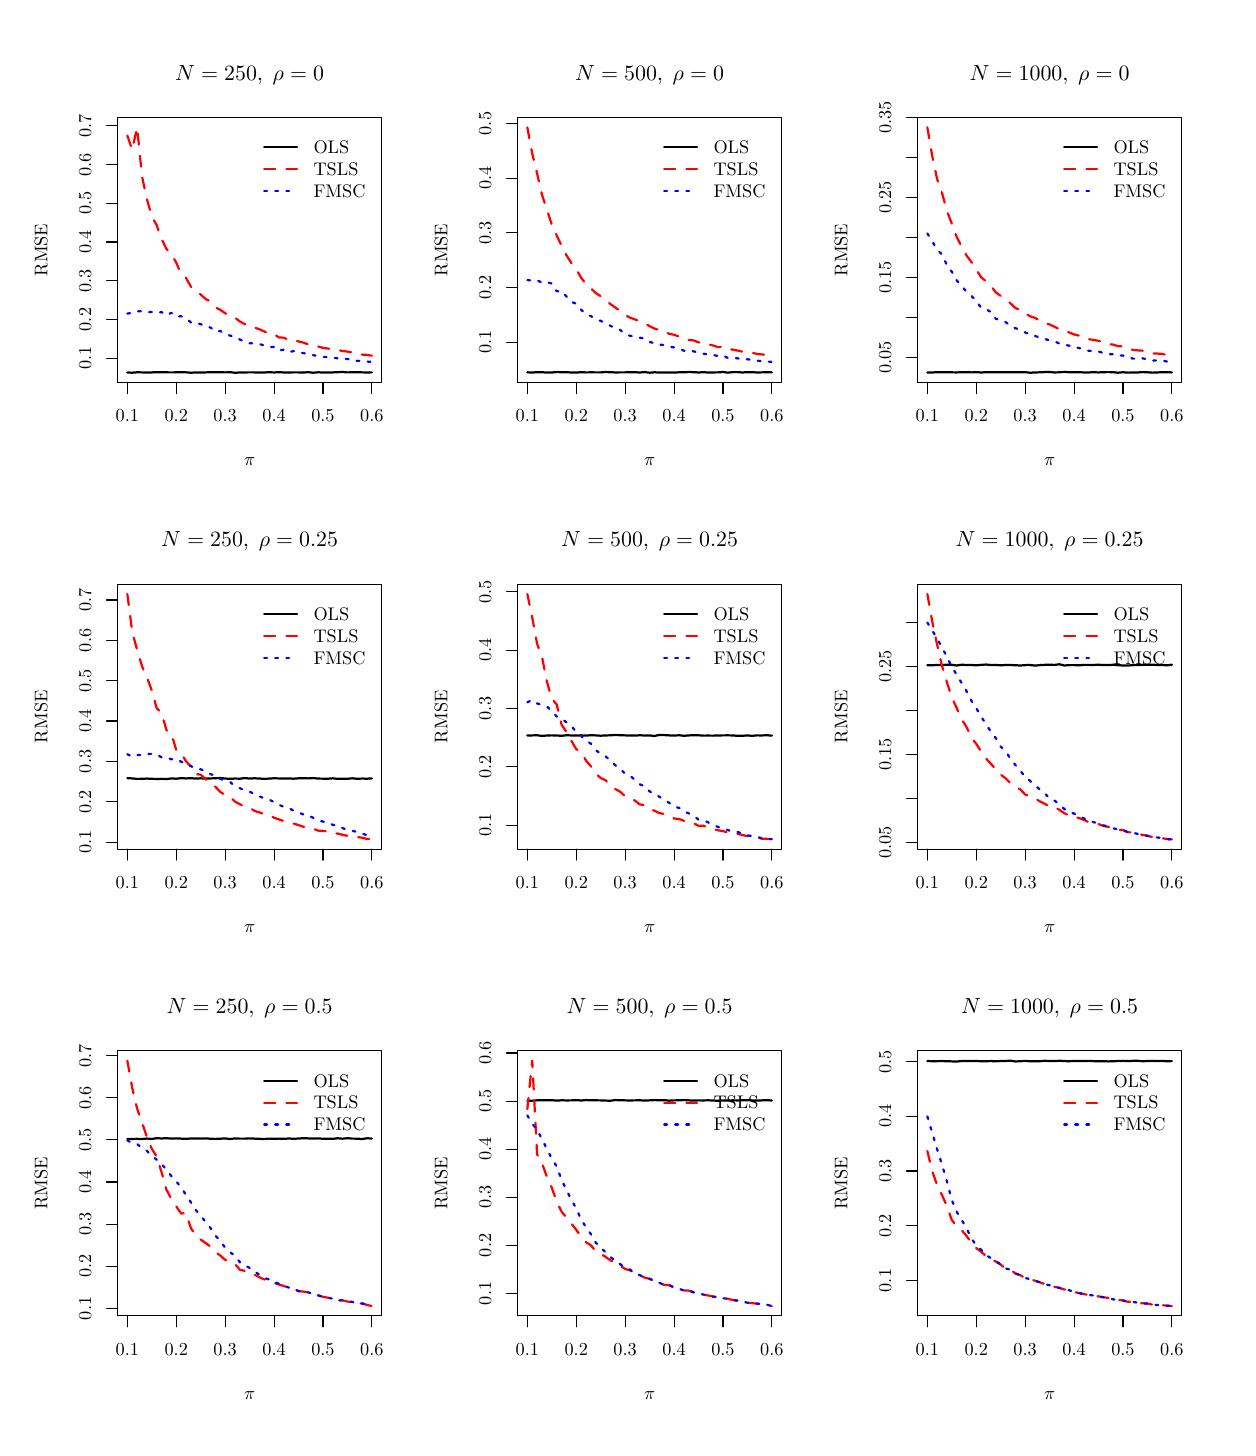
\begin{tikzpicture}[x=1pt,y=1pt]
\definecolor[named]{fillColor}{rgb}{1.00,1.00,1.00}
\path[use as bounding box,fill=fillColor,fill opacity=0.00] (0,0) rectangle (433.62,505.89);
\begin{scope}
\path[clip] ( 32.47,377.65) rectangle (127.91,473.42);
\definecolor[named]{drawColor}{rgb}{0.00,0.00,0.00}

\path[draw=drawColor,line width= 0.8pt,line join=round,line cap=round] ( 36.01,381.28) --
	( 37.77,381.21) --
	( 39.54,381.36) --
	( 41.31,381.32) --
	( 43.08,381.27) --
	( 44.84,381.31) --
	( 46.61,381.41) --
	( 48.38,381.34) --
	( 50.15,381.34) --
	( 51.91,381.32) --
	( 53.68,381.34) --
	( 55.45,381.35) --
	( 57.21,381.34) --
	( 58.98,381.20) --
	( 60.75,381.31) --
	( 62.52,381.29) --
	( 64.28,381.32) --
	( 66.05,381.38) --
	( 67.82,381.35) --
	( 69.59,381.41) --
	( 71.35,381.32) --
	( 73.12,381.40) --
	( 74.89,381.20) --
	( 76.66,381.27) --
	( 78.42,381.31) --
	( 80.19,381.33) --
	( 81.96,381.32) --
	( 83.72,381.27) --
	( 85.49,381.30) --
	( 87.26,381.38) --
	( 89.03,381.30) --
	( 90.79,381.39) --
	( 92.56,381.30) --
	( 94.33,381.29) --
	( 96.10,381.33) --
	( 97.86,381.32) --
	( 99.63,381.28) --
	(101.40,381.38) --
	(103.17,381.20) --
	(104.93,381.35) --
	(106.70,381.29) --
	(108.47,381.25) --
	(110.23,381.32) --
	(112.00,381.40) --
	(113.77,381.47) --
	(115.54,381.33) --
	(117.30,381.34) --
	(119.07,381.38) --
	(120.84,381.33) --
	(122.61,381.30) --
	(124.37,381.33);
\end{scope}
\begin{scope}
\path[clip] (  0.00,  0.00) rectangle (433.62,505.89);
\definecolor[named]{drawColor}{rgb}{0.00,0.00,0.00}

\path[draw=drawColor,line width= 0.4pt,line join=round,line cap=round] ( 36.01,377.65) -- (124.37,377.65);

\path[draw=drawColor,line width= 0.4pt,line join=round,line cap=round] ( 36.01,377.65) -- ( 36.01,373.69);

\path[draw=drawColor,line width= 0.4pt,line join=round,line cap=round] ( 53.68,377.65) -- ( 53.68,373.69);

\path[draw=drawColor,line width= 0.4pt,line join=round,line cap=round] ( 71.35,377.65) -- ( 71.35,373.69);

\path[draw=drawColor,line width= 0.4pt,line join=round,line cap=round] ( 89.03,377.65) -- ( 89.03,373.69);

\path[draw=drawColor,line width= 0.4pt,line join=round,line cap=round] (106.70,377.65) -- (106.70,373.69);

\path[draw=drawColor,line width= 0.4pt,line join=round,line cap=round] (124.37,377.65) -- (124.37,373.69);

\node[text=drawColor,anchor=base,inner sep=0pt, outer sep=0pt, scale=  0.66] at ( 36.01,363.40) {0.1};

\node[text=drawColor,anchor=base,inner sep=0pt, outer sep=0pt, scale=  0.66] at ( 53.68,363.40) {0.2};

\node[text=drawColor,anchor=base,inner sep=0pt, outer sep=0pt, scale=  0.66] at ( 71.35,363.40) {0.3};

\node[text=drawColor,anchor=base,inner sep=0pt, outer sep=0pt, scale=  0.66] at ( 89.03,363.40) {0.4};

\node[text=drawColor,anchor=base,inner sep=0pt, outer sep=0pt, scale=  0.66] at (106.70,363.40) {0.5};

\node[text=drawColor,anchor=base,inner sep=0pt, outer sep=0pt, scale=  0.66] at (124.37,363.40) {0.6};

\path[draw=drawColor,line width= 0.4pt,line join=round,line cap=round] ( 32.47,386.43) -- ( 32.47,470.42);

\path[draw=drawColor,line width= 0.4pt,line join=round,line cap=round] ( 32.47,386.43) -- ( 28.51,386.43);

\path[draw=drawColor,line width= 0.4pt,line join=round,line cap=round] ( 32.47,400.43) -- ( 28.51,400.43);

\path[draw=drawColor,line width= 0.4pt,line join=round,line cap=round] ( 32.47,414.43) -- ( 28.51,414.43);

\path[draw=drawColor,line width= 0.4pt,line join=round,line cap=round] ( 32.47,428.43) -- ( 28.51,428.43);

\path[draw=drawColor,line width= 0.4pt,line join=round,line cap=round] ( 32.47,442.43) -- ( 28.51,442.43);

\path[draw=drawColor,line width= 0.4pt,line join=round,line cap=round] ( 32.47,456.42) -- ( 28.51,456.42);

\path[draw=drawColor,line width= 0.4pt,line join=round,line cap=round] ( 32.47,470.42) -- ( 28.51,470.42);

\node[text=drawColor,rotate= 90.00,anchor=base,inner sep=0pt, outer sep=0pt, scale=  0.66] at ( 22.97,386.43) {0.1};

\node[text=drawColor,rotate= 90.00,anchor=base,inner sep=0pt, outer sep=0pt, scale=  0.66] at ( 22.97,400.43) {0.2};

\node[text=drawColor,rotate= 90.00,anchor=base,inner sep=0pt, outer sep=0pt, scale=  0.66] at ( 22.97,414.43) {0.3};

\node[text=drawColor,rotate= 90.00,anchor=base,inner sep=0pt, outer sep=0pt, scale=  0.66] at ( 22.97,428.43) {0.4};

\node[text=drawColor,rotate= 90.00,anchor=base,inner sep=0pt, outer sep=0pt, scale=  0.66] at ( 22.97,442.43) {0.5};

\node[text=drawColor,rotate= 90.00,anchor=base,inner sep=0pt, outer sep=0pt, scale=  0.66] at ( 22.97,456.42) {0.6};

\node[text=drawColor,rotate= 90.00,anchor=base,inner sep=0pt, outer sep=0pt, scale=  0.66] at ( 22.97,470.42) {0.7};

\path[draw=drawColor,line width= 0.4pt,line join=round,line cap=round] ( 32.47,377.65) --
	(127.91,377.65) --
	(127.91,473.42) --
	( 32.47,473.42) --
	( 32.47,377.65);
\end{scope}
\begin{scope}
\path[clip] (  0.00,337.26) rectangle (144.54,505.89);
\definecolor[named]{drawColor}{rgb}{0.00,0.00,0.00}

\node[text=drawColor,anchor=base,inner sep=0pt, outer sep=0pt, scale=  0.79] at ( 80.19,486.92) {\bfseries $N=250, \;\rho=0$};

\node[text=drawColor,anchor=base,inner sep=0pt, outer sep=0pt, scale=  0.66] at ( 80.19,347.56) {$\pi$};

\node[text=drawColor,rotate= 90.00,anchor=base,inner sep=0pt, outer sep=0pt, scale=  0.66] at (  7.13,425.53) {RMSE};
\end{scope}
\begin{scope}
\path[clip] ( 32.47,377.65) rectangle (127.91,473.42);
\definecolor[named]{drawColor}{rgb}{1.00,0.00,0.00}

\path[draw=drawColor,line width= 0.8pt,dash pattern=on 4pt off 4pt ,line join=round,line cap=round] ( 36.01,466.90) --
	( 37.77,461.77) --
	( 39.54,469.87) --
	( 41.31,452.21) --
	( 43.08,443.93) --
	( 44.84,437.71) --
	( 46.61,434.52) --
	( 48.38,429.50) --
	( 50.15,425.93) --
	( 51.91,424.10) --
	( 53.68,420.96) --
	( 55.45,416.99) --
	( 57.21,415.46) --
	( 58.98,412.33) --
	( 60.75,410.79) --
	( 62.52,409.47) --
	( 64.28,407.85) --
	( 66.05,406.94) --
	( 67.82,404.82) --
	( 69.59,403.93) --
	( 71.35,402.71) --
	( 73.12,401.68) --
	( 74.89,401.08) --
	( 76.66,399.74) --
	( 78.42,398.79) --
	( 80.19,397.80) --
	( 81.96,397.51) --
	( 83.72,396.91) --
	( 85.49,396.12) --
	( 87.26,395.31) --
	( 89.03,395.19) --
	( 90.79,393.94) --
	( 92.56,393.87) --
	( 94.33,393.00) --
	( 96.10,393.04) --
	( 97.86,392.50) --
	( 99.63,392.08) --
	(101.40,391.47) --
	(103.17,391.07) --
	(104.93,390.70) --
	(106.70,390.17) --
	(108.47,389.94) --
	(110.23,389.63) --
	(112.00,389.41) --
	(113.77,389.06) --
	(115.54,388.83) --
	(117.30,388.55) --
	(119.07,388.06) --
	(120.84,387.77) --
	(122.61,387.62) --
	(124.37,387.36);
\definecolor[named]{drawColor}{rgb}{0.00,0.00,1.00}

\path[draw=drawColor,line width= 0.8pt,dash pattern=on 1pt off 3pt ,line join=round,line cap=round] ( 36.01,402.56) --
	( 37.77,402.87) --
	( 39.54,403.36) --
	( 41.31,403.47) --
	( 43.08,403.12) --
	( 44.84,403.14) --
	( 46.61,402.82) --
	( 48.38,403.13) --
	( 50.15,401.89) --
	( 51.91,402.85) --
	( 53.68,401.46) --
	( 55.45,401.61) --
	( 57.21,400.92) --
	( 58.98,399.37) --
	( 60.75,399.19) --
	( 62.52,398.76) --
	( 64.28,397.82) --
	( 66.05,397.55) --
	( 67.82,396.06) --
	( 69.59,396.28) --
	( 71.35,395.10) --
	( 73.12,394.62) --
	( 74.89,394.18) --
	( 76.66,393.20) --
	( 78.42,392.47) --
	( 80.19,391.83) --
	( 81.96,391.79) --
	( 83.72,391.56) --
	( 85.49,391.06) --
	( 87.26,390.48) --
	( 89.03,390.54) --
	( 90.79,389.21) --
	( 92.56,389.54) --
	( 94.33,388.62) --
	( 96.10,389.01) --
	( 97.86,388.57) --
	( 99.63,388.29) --
	(101.40,387.97) --
	(103.17,387.55) --
	(104.93,387.18) --
	(106.70,386.95) --
	(108.47,386.80) --
	(110.23,386.52) --
	(112.00,386.45) --
	(113.77,386.35) --
	(115.54,386.13) --
	(117.30,386.00) --
	(119.07,385.50) --
	(120.84,385.44) --
	(122.61,385.24) --
	(124.37,385.10);
\definecolor[named]{drawColor}{rgb}{0.00,0.00,0.00}

\path[draw=drawColor,line width= 0.8pt,line join=round,line cap=round] ( 85.47,462.63) -- ( 97.35,462.63);
\definecolor[named]{drawColor}{rgb}{1.00,0.00,0.00}

\path[draw=drawColor,line width= 0.8pt,dash pattern=on 4pt off 4pt ,line join=round,line cap=round] ( 85.47,454.71) -- ( 97.35,454.71);
\definecolor[named]{drawColor}{rgb}{0.00,0.00,1.00}

\path[draw=drawColor,line width= 0.8pt,dash pattern=on 1pt off 3pt ,line join=round,line cap=round] ( 85.47,446.79) -- ( 97.35,446.79);
\definecolor[named]{drawColor}{rgb}{0.00,0.00,0.00}

\node[text=drawColor,anchor=base west,inner sep=0pt, outer sep=0pt, scale=  0.66] at (103.29,460.35) {OLS};

\node[text=drawColor,anchor=base west,inner sep=0pt, outer sep=0pt, scale=  0.66] at (103.29,452.43) {TSLS};

\node[text=drawColor,anchor=base west,inner sep=0pt, outer sep=0pt, scale=  0.66] at (103.29,444.51) {FMSC};
\end{scope}
\begin{scope}
\path[clip] (177.01,377.65) rectangle (272.45,473.42);
\definecolor[named]{drawColor}{rgb}{0.00,0.00,0.00}

\path[draw=drawColor,line width= 0.8pt,line join=round,line cap=round] (180.55,381.35) --
	(182.31,381.27) --
	(184.08,381.41) --
	(185.85,381.36) --
	(187.62,381.28) --
	(189.38,381.28) --
	(191.15,381.46) --
	(192.92,381.37) --
	(194.69,381.36) --
	(196.45,381.30) --
	(198.22,381.25) --
	(199.99,381.38) --
	(201.75,381.32) --
	(203.52,381.34) --
	(205.29,381.33) --
	(207.06,381.32) --
	(208.82,381.45) --
	(210.59,381.38) --
	(212.36,381.30) --
	(214.13,381.33) --
	(215.89,381.33) --
	(217.66,381.39) --
	(219.43,381.38) --
	(221.20,381.28) --
	(222.96,381.44) --
	(224.73,381.20) --
	(226.50,381.36) --
	(228.26,381.27) --
	(230.03,381.32) --
	(231.80,381.28) --
	(233.57,381.26) --
	(235.33,381.35) --
	(237.10,381.36) --
	(238.87,381.44) --
	(240.64,381.40) --
	(242.40,381.29) --
	(244.17,381.39) --
	(245.94,381.28) --
	(247.71,381.31) --
	(249.47,381.33) --
	(251.24,381.47) --
	(253.01,381.22) --
	(254.77,381.41) --
	(256.54,381.42) --
	(258.31,381.29) --
	(260.08,381.40) --
	(261.84,381.39) --
	(263.61,381.29) --
	(265.38,381.33) --
	(267.15,381.38) --
	(268.91,381.35);
\end{scope}
\begin{scope}
\path[clip] (  0.00,  0.00) rectangle (433.62,505.89);
\definecolor[named]{drawColor}{rgb}{0.00,0.00,0.00}

\path[draw=drawColor,line width= 0.4pt,line join=round,line cap=round] (180.55,377.65) -- (268.91,377.65);

\path[draw=drawColor,line width= 0.4pt,line join=round,line cap=round] (180.55,377.65) -- (180.55,373.69);

\path[draw=drawColor,line width= 0.4pt,line join=round,line cap=round] (198.22,377.65) -- (198.22,373.69);

\path[draw=drawColor,line width= 0.4pt,line join=round,line cap=round] (215.89,377.65) -- (215.89,373.69);

\path[draw=drawColor,line width= 0.4pt,line join=round,line cap=round] (233.57,377.65) -- (233.57,373.69);

\path[draw=drawColor,line width= 0.4pt,line join=round,line cap=round] (251.24,377.65) -- (251.24,373.69);

\path[draw=drawColor,line width= 0.4pt,line join=round,line cap=round] (268.91,377.65) -- (268.91,373.69);

\node[text=drawColor,anchor=base,inner sep=0pt, outer sep=0pt, scale=  0.66] at (180.55,363.40) {0.1};

\node[text=drawColor,anchor=base,inner sep=0pt, outer sep=0pt, scale=  0.66] at (198.22,363.40) {0.2};

\node[text=drawColor,anchor=base,inner sep=0pt, outer sep=0pt, scale=  0.66] at (215.89,363.40) {0.3};

\node[text=drawColor,anchor=base,inner sep=0pt, outer sep=0pt, scale=  0.66] at (233.57,363.40) {0.4};

\node[text=drawColor,anchor=base,inner sep=0pt, outer sep=0pt, scale=  0.66] at (251.24,363.40) {0.5};

\node[text=drawColor,anchor=base,inner sep=0pt, outer sep=0pt, scale=  0.66] at (268.91,363.40) {0.6};

\path[draw=drawColor,line width= 0.4pt,line join=round,line cap=round] (177.01,392.25) -- (177.01,471.27);

\path[draw=drawColor,line width= 0.4pt,line join=round,line cap=round] (177.01,392.25) -- (173.05,392.25);

\path[draw=drawColor,line width= 0.4pt,line join=round,line cap=round] (177.01,412.01) -- (173.05,412.01);

\path[draw=drawColor,line width= 0.4pt,line join=round,line cap=round] (177.01,431.76) -- (173.05,431.76);

\path[draw=drawColor,line width= 0.4pt,line join=round,line cap=round] (177.01,451.52) -- (173.05,451.52);

\path[draw=drawColor,line width= 0.4pt,line join=round,line cap=round] (177.01,471.27) -- (173.05,471.27);

\node[text=drawColor,rotate= 90.00,anchor=base,inner sep=0pt, outer sep=0pt, scale=  0.66] at (167.51,392.25) {0.1};

\node[text=drawColor,rotate= 90.00,anchor=base,inner sep=0pt, outer sep=0pt, scale=  0.66] at (167.51,412.01) {0.2};

\node[text=drawColor,rotate= 90.00,anchor=base,inner sep=0pt, outer sep=0pt, scale=  0.66] at (167.51,431.76) {0.3};

\node[text=drawColor,rotate= 90.00,anchor=base,inner sep=0pt, outer sep=0pt, scale=  0.66] at (167.51,451.52) {0.4};

\node[text=drawColor,rotate= 90.00,anchor=base,inner sep=0pt, outer sep=0pt, scale=  0.66] at (167.51,471.27) {0.5};

\path[draw=drawColor,line width= 0.4pt,line join=round,line cap=round] (177.01,377.65) --
	(272.45,377.65) --
	(272.45,473.42) --
	(177.01,473.42) --
	(177.01,377.65);
\end{scope}
\begin{scope}
\path[clip] (144.54,337.26) rectangle (289.08,505.89);
\definecolor[named]{drawColor}{rgb}{0.00,0.00,0.00}

\node[text=drawColor,anchor=base,inner sep=0pt, outer sep=0pt, scale=  0.79] at (224.73,486.92) {\bfseries $N=500, \;\rho=0$};

\node[text=drawColor,anchor=base,inner sep=0pt, outer sep=0pt, scale=  0.66] at (224.73,347.56) {$\pi$};

\node[text=drawColor,rotate= 90.00,anchor=base,inner sep=0pt, outer sep=0pt, scale=  0.66] at (151.67,425.53) {RMSE};
\end{scope}
\begin{scope}
\path[clip] (177.01,377.65) rectangle (272.45,473.42);
\definecolor[named]{drawColor}{rgb}{1.00,0.00,0.00}

\path[draw=drawColor,line width= 0.8pt,dash pattern=on 4pt off 4pt ,line join=round,line cap=round] (180.55,469.87) --
	(182.31,460.41) --
	(184.08,453.21) --
	(185.85,445.46) --
	(187.62,440.10) --
	(189.38,434.78) --
	(191.15,430.82) --
	(192.92,427.12) --
	(194.69,423.65) --
	(196.45,420.82) --
	(198.22,418.57) --
	(199.99,415.52) --
	(201.75,413.23) --
	(203.52,411.66) --
	(205.29,409.99) --
	(207.06,408.86) --
	(208.82,407.34) --
	(210.59,405.99) --
	(212.36,404.74) --
	(214.13,403.52) --
	(215.89,402.02) --
	(217.66,401.10) --
	(219.43,400.45) --
	(221.20,399.82) --
	(222.96,399.09) --
	(224.73,398.02) --
	(226.50,397.16) --
	(228.26,396.61) --
	(230.03,395.99) --
	(231.80,395.28) --
	(233.57,394.92) --
	(235.33,394.28) --
	(237.10,393.38) --
	(238.87,393.02) --
	(240.64,392.87) --
	(242.40,392.18) --
	(244.17,391.74) --
	(245.94,391.47) --
	(247.71,391.03) --
	(249.47,390.46) --
	(251.24,390.62) --
	(253.01,389.73) --
	(254.77,389.56) --
	(256.54,389.21) --
	(258.31,388.80) --
	(260.08,388.69) --
	(261.84,388.38) --
	(263.61,387.99) --
	(265.38,387.81) --
	(267.15,387.58) --
	(268.91,387.30);
\definecolor[named]{drawColor}{rgb}{0.00,0.00,1.00}

\path[draw=drawColor,line width= 0.8pt,dash pattern=on 1pt off 3pt ,line join=round,line cap=round] (180.55,414.68) --
	(182.31,414.53) --
	(184.08,414.62) --
	(185.85,413.72) --
	(187.62,413.92) --
	(189.38,413.42) --
	(191.15,410.65) --
	(192.92,410.73) --
	(194.69,408.76) --
	(196.45,406.83) --
	(198.22,406.11) --
	(199.99,403.96) --
	(201.75,402.36) --
	(203.52,401.66) --
	(205.29,400.62) --
	(207.06,399.93) --
	(208.82,399.12) --
	(210.59,398.13) --
	(212.36,397.28) --
	(214.13,396.65) --
	(215.89,395.09) --
	(217.66,394.54) --
	(219.43,394.23) --
	(221.20,393.85) --
	(222.96,393.49) --
	(224.73,392.33) --
	(226.50,391.84) --
	(228.26,391.36) --
	(230.03,391.19) --
	(231.80,390.58) --
	(233.57,390.34) --
	(235.33,389.94) --
	(237.10,389.16) --
	(238.87,388.91) --
	(240.64,388.94) --
	(242.40,388.37) --
	(244.17,388.05) --
	(245.94,387.86) --
	(247.71,387.63) --
	(249.47,387.22) --
	(251.24,387.39) --
	(253.01,386.54) --
	(254.77,386.69) --
	(256.54,386.39) --
	(258.31,385.99) --
	(260.08,386.07) --
	(261.84,385.77) --
	(263.61,385.53) --
	(265.38,385.40) --
	(267.15,385.29) --
	(268.91,385.10);
\definecolor[named]{drawColor}{rgb}{0.00,0.00,0.00}

\path[draw=drawColor,line width= 0.8pt,line join=round,line cap=round] (230.01,462.63) -- (241.89,462.63);
\definecolor[named]{drawColor}{rgb}{1.00,0.00,0.00}

\path[draw=drawColor,line width= 0.8pt,dash pattern=on 4pt off 4pt ,line join=round,line cap=round] (230.01,454.71) -- (241.89,454.71);
\definecolor[named]{drawColor}{rgb}{0.00,0.00,1.00}

\path[draw=drawColor,line width= 0.8pt,dash pattern=on 1pt off 3pt ,line join=round,line cap=round] (230.01,446.79) -- (241.89,446.79);
\definecolor[named]{drawColor}{rgb}{0.00,0.00,0.00}

\node[text=drawColor,anchor=base west,inner sep=0pt, outer sep=0pt, scale=  0.66] at (247.83,460.35) {OLS};

\node[text=drawColor,anchor=base west,inner sep=0pt, outer sep=0pt, scale=  0.66] at (247.83,452.43) {TSLS};

\node[text=drawColor,anchor=base west,inner sep=0pt, outer sep=0pt, scale=  0.66] at (247.83,444.51) {FMSC};
\end{scope}
\begin{scope}
\path[clip] (321.55,377.65) rectangle (416.99,473.42);
\definecolor[named]{drawColor}{rgb}{0.00,0.00,0.00}

\path[draw=drawColor,line width= 0.8pt,line join=round,line cap=round] (325.09,381.27) --
	(326.85,381.29) --
	(328.62,381.40) --
	(330.39,381.35) --
	(332.16,381.36) --
	(333.92,381.34) --
	(335.69,381.31) --
	(337.46,381.41) --
	(339.23,381.41) --
	(340.99,381.32) --
	(342.76,381.41) --
	(344.53,381.29) --
	(346.29,381.38) --
	(348.06,381.39) --
	(349.83,381.40) --
	(351.60,381.36) --
	(353.36,381.34) --
	(355.13,381.35) --
	(356.90,381.38) --
	(358.67,381.39) --
	(360.43,381.41) --
	(362.20,381.20) --
	(363.97,381.30) --
	(365.74,381.34) --
	(367.50,381.44) --
	(369.27,381.48) --
	(371.04,381.30) --
	(372.80,381.35) --
	(374.57,381.52) --
	(376.34,381.36) --
	(378.11,381.36) --
	(379.87,381.39) --
	(381.64,381.31) --
	(383.41,381.31) --
	(385.18,381.37) --
	(386.94,381.31) --
	(388.71,381.40) --
	(390.48,381.42) --
	(392.25,381.38) --
	(394.01,381.21) --
	(395.78,381.37) --
	(397.55,381.23) --
	(399.31,381.28) --
	(401.08,381.29) --
	(402.85,381.43) --
	(404.62,381.36) --
	(406.38,381.23) --
	(408.15,381.30) --
	(409.92,381.38) --
	(411.69,381.40) --
	(413.45,381.31);
\end{scope}
\begin{scope}
\path[clip] (  0.00,  0.00) rectangle (433.62,505.89);
\definecolor[named]{drawColor}{rgb}{0.00,0.00,0.00}

\path[draw=drawColor,line width= 0.4pt,line join=round,line cap=round] (325.09,377.65) -- (413.45,377.65);

\path[draw=drawColor,line width= 0.4pt,line join=round,line cap=round] (325.09,377.65) -- (325.09,373.69);

\path[draw=drawColor,line width= 0.4pt,line join=round,line cap=round] (342.76,377.65) -- (342.76,373.69);

\path[draw=drawColor,line width= 0.4pt,line join=round,line cap=round] (360.43,377.65) -- (360.43,373.69);

\path[draw=drawColor,line width= 0.4pt,line join=round,line cap=round] (378.11,377.65) -- (378.11,373.69);

\path[draw=drawColor,line width= 0.4pt,line join=round,line cap=round] (395.78,377.65) -- (395.78,373.69);

\path[draw=drawColor,line width= 0.4pt,line join=round,line cap=round] (413.45,377.65) -- (413.45,373.69);

\node[text=drawColor,anchor=base,inner sep=0pt, outer sep=0pt, scale=  0.66] at (325.09,363.40) {0.1};

\node[text=drawColor,anchor=base,inner sep=0pt, outer sep=0pt, scale=  0.66] at (342.76,363.40) {0.2};

\node[text=drawColor,anchor=base,inner sep=0pt, outer sep=0pt, scale=  0.66] at (360.43,363.40) {0.3};

\node[text=drawColor,anchor=base,inner sep=0pt, outer sep=0pt, scale=  0.66] at (378.11,363.40) {0.4};

\node[text=drawColor,anchor=base,inner sep=0pt, outer sep=0pt, scale=  0.66] at (395.78,363.40) {0.5};

\node[text=drawColor,anchor=base,inner sep=0pt, outer sep=0pt, scale=  0.66] at (413.45,363.40) {0.6};

\path[draw=drawColor,line width= 0.4pt,line join=round,line cap=round] (321.55,386.65) -- (321.55,473.35);

\path[draw=drawColor,line width= 0.4pt,line join=round,line cap=round] (321.55,386.65) -- (317.59,386.65);

\path[draw=drawColor,line width= 0.4pt,line join=round,line cap=round] (321.55,401.10) -- (317.59,401.10);

\path[draw=drawColor,line width= 0.4pt,line join=round,line cap=round] (321.55,415.55) -- (317.59,415.55);

\path[draw=drawColor,line width= 0.4pt,line join=round,line cap=round] (321.55,430.00) -- (317.59,430.00);

\path[draw=drawColor,line width= 0.4pt,line join=round,line cap=round] (321.55,444.45) -- (317.59,444.45);

\path[draw=drawColor,line width= 0.4pt,line join=round,line cap=round] (321.55,458.90) -- (317.59,458.90);

\path[draw=drawColor,line width= 0.4pt,line join=round,line cap=round] (321.55,473.35) -- (317.59,473.35);

\node[text=drawColor,rotate= 90.00,anchor=base,inner sep=0pt, outer sep=0pt, scale=  0.66] at (312.05,386.65) {0.05};

\node[text=drawColor,rotate= 90.00,anchor=base,inner sep=0pt, outer sep=0pt, scale=  0.66] at (312.05,415.55) {0.15};

\node[text=drawColor,rotate= 90.00,anchor=base,inner sep=0pt, outer sep=0pt, scale=  0.66] at (312.05,444.45) {0.25};

\node[text=drawColor,rotate= 90.00,anchor=base,inner sep=0pt, outer sep=0pt, scale=  0.66] at (312.05,473.35) {0.35};

\path[draw=drawColor,line width= 0.4pt,line join=round,line cap=round] (321.55,377.65) --
	(416.99,377.65) --
	(416.99,473.42) --
	(321.55,473.42) --
	(321.55,377.65);
\end{scope}
\begin{scope}
\path[clip] (289.08,337.26) rectangle (433.62,505.89);
\definecolor[named]{drawColor}{rgb}{0.00,0.00,0.00}

\node[text=drawColor,anchor=base,inner sep=0pt, outer sep=0pt, scale=  0.79] at (369.27,486.92) {\bfseries $N=1000, \;\rho=0$};

\node[text=drawColor,anchor=base,inner sep=0pt, outer sep=0pt, scale=  0.66] at (369.27,347.56) {$\pi$};

\node[text=drawColor,rotate= 90.00,anchor=base,inner sep=0pt, outer sep=0pt, scale=  0.66] at (296.21,425.53) {RMSE};
\end{scope}
\begin{scope}
\path[clip] (321.55,377.65) rectangle (416.99,473.42);
\definecolor[named]{drawColor}{rgb}{1.00,0.00,0.00}

\path[draw=drawColor,line width= 0.8pt,dash pattern=on 4pt off 4pt ,line join=round,line cap=round] (325.09,469.87) --
	(326.85,459.55) --
	(328.62,451.20) --
	(330.39,446.20) --
	(332.16,439.70) --
	(333.92,435.07) --
	(335.69,430.30) --
	(337.46,426.80) --
	(339.23,423.59) --
	(340.99,421.24) --
	(342.76,418.49) --
	(344.53,415.67) --
	(346.29,414.26) --
	(348.06,412.60) --
	(349.83,410.21) --
	(351.60,408.99) --
	(353.36,407.81) --
	(355.13,406.28) --
	(356.90,404.59) --
	(358.67,403.90) --
	(360.43,402.60) --
	(362.20,401.63) --
	(363.97,401.04) --
	(365.74,400.01) --
	(367.50,399.22) --
	(369.27,398.62) --
	(371.04,397.80) --
	(372.80,396.92) --
	(374.57,396.26) --
	(376.34,395.75) --
	(378.11,395.05) --
	(379.87,394.60) --
	(381.64,393.84) --
	(383.41,393.32) --
	(385.18,393.04) --
	(386.94,392.74) --
	(388.71,392.11) --
	(390.48,391.59) --
	(392.25,391.35) --
	(394.01,390.80) --
	(395.78,390.67) --
	(397.55,390.24) --
	(399.31,389.45) --
	(401.08,389.28) --
	(402.85,389.17) --
	(404.62,388.81) --
	(406.38,388.21) --
	(408.15,388.12) --
	(409.92,387.99) --
	(411.69,387.57) --
	(413.45,387.36);
\definecolor[named]{drawColor}{rgb}{0.00,0.00,1.00}

\path[draw=drawColor,line width= 0.8pt,dash pattern=on 1pt off 3pt ,line join=round,line cap=round] (325.09,431.52) --
	(326.85,428.76) --
	(328.62,425.55) --
	(330.39,423.97) --
	(332.16,420.11) --
	(333.92,417.72) --
	(335.69,414.57) --
	(337.46,412.58) --
	(339.23,410.45) --
	(340.99,408.96) --
	(342.76,407.18) --
	(344.53,404.61) --
	(346.29,404.17) --
	(348.06,403.13) --
	(349.83,400.69) --
	(351.60,400.18) --
	(353.36,399.48) --
	(355.13,398.16) --
	(356.90,397.27) --
	(358.67,396.79) --
	(360.43,395.77) --
	(362.20,395.05) --
	(363.97,394.50) --
	(365.74,393.93) --
	(367.50,393.42) --
	(369.27,392.86) --
	(371.04,392.54) --
	(372.80,391.74) --
	(374.57,391.36) --
	(376.34,390.96) --
	(378.11,390.35) --
	(379.87,390.16) --
	(381.64,389.41) --
	(383.41,389.12) --
	(385.18,389.04) --
	(386.94,388.88) --
	(388.71,388.28) --
	(390.48,387.92) --
	(392.25,387.87) --
	(394.01,387.46) --
	(395.78,387.39) --
	(397.55,387.12) --
	(399.31,386.29) --
	(401.08,386.32) --
	(402.85,386.40) --
	(404.62,386.00) --
	(406.38,385.64) --
	(408.15,385.66) --
	(409.92,385.59) --
	(411.69,385.23) --
	(413.45,385.09);
\definecolor[named]{drawColor}{rgb}{0.00,0.00,0.00}

\path[draw=drawColor,line width= 0.8pt,line join=round,line cap=round] (374.55,462.63) -- (386.43,462.63);
\definecolor[named]{drawColor}{rgb}{1.00,0.00,0.00}

\path[draw=drawColor,line width= 0.8pt,dash pattern=on 4pt off 4pt ,line join=round,line cap=round] (374.55,454.71) -- (386.43,454.71);
\definecolor[named]{drawColor}{rgb}{0.00,0.00,1.00}

\path[draw=drawColor,line width= 0.8pt,dash pattern=on 1pt off 3pt ,line join=round,line cap=round] (374.55,446.79) -- (386.43,446.79);
\definecolor[named]{drawColor}{rgb}{0.00,0.00,0.00}

\node[text=drawColor,anchor=base west,inner sep=0pt, outer sep=0pt, scale=  0.66] at (392.37,460.35) {OLS};

\node[text=drawColor,anchor=base west,inner sep=0pt, outer sep=0pt, scale=  0.66] at (392.37,452.43) {TSLS};

\node[text=drawColor,anchor=base west,inner sep=0pt, outer sep=0pt, scale=  0.66] at (392.37,444.51) {FMSC};
\end{scope}
\begin{scope}
\path[clip] ( 32.47,209.02) rectangle (127.91,304.79);
\definecolor[named]{drawColor}{rgb}{0.00,0.00,0.00}

\path[draw=drawColor,line width= 0.8pt,line join=round,line cap=round] ( 36.01,234.72) --
	( 37.77,234.60) --
	( 39.54,234.43) --
	( 41.31,234.46) --
	( 43.08,234.55) --
	( 44.84,234.47) --
	( 46.61,234.40) --
	( 48.38,234.45) --
	( 50.15,234.38) --
	( 51.91,234.59) --
	( 53.68,234.50) --
	( 55.45,234.69) --
	( 57.21,234.60) --
	( 58.98,234.70) --
	( 60.75,234.55) --
	( 62.52,234.64) --
	( 64.28,234.54) --
	( 66.05,234.61) --
	( 67.82,234.65) --
	( 69.59,234.75) --
	( 71.35,234.57) --
	( 73.12,234.45) --
	( 74.89,234.56) --
	( 76.66,234.50) --
	( 78.42,234.73) --
	( 80.19,234.56) --
	( 81.96,234.65) --
	( 83.72,234.57) --
	( 85.49,234.43) --
	( 87.26,234.55) --
	( 89.03,234.65) --
	( 90.79,234.61) --
	( 92.56,234.56) --
	( 94.33,234.58) --
	( 96.10,234.51) --
	( 97.86,234.64) --
	( 99.63,234.66) --
	(101.40,234.62) --
	(103.17,234.73) --
	(104.93,234.55) --
	(106.70,234.52) --
	(108.47,234.49) --
	(110.23,234.64) --
	(112.00,234.44) --
	(113.77,234.51) --
	(115.54,234.46) --
	(117.30,234.65) --
	(119.07,234.47) --
	(120.84,234.55) --
	(122.61,234.50) --
	(124.37,234.62);
\end{scope}
\begin{scope}
\path[clip] (  0.00,  0.00) rectangle (433.62,505.89);
\definecolor[named]{drawColor}{rgb}{0.00,0.00,0.00}

\path[draw=drawColor,line width= 0.4pt,line join=round,line cap=round] ( 36.01,209.02) -- (124.37,209.02);

\path[draw=drawColor,line width= 0.4pt,line join=round,line cap=round] ( 36.01,209.02) -- ( 36.01,205.06);

\path[draw=drawColor,line width= 0.4pt,line join=round,line cap=round] ( 53.68,209.02) -- ( 53.68,205.06);

\path[draw=drawColor,line width= 0.4pt,line join=round,line cap=round] ( 71.35,209.02) -- ( 71.35,205.06);

\path[draw=drawColor,line width= 0.4pt,line join=round,line cap=round] ( 89.03,209.02) -- ( 89.03,205.06);

\path[draw=drawColor,line width= 0.4pt,line join=round,line cap=round] (106.70,209.02) -- (106.70,205.06);

\path[draw=drawColor,line width= 0.4pt,line join=round,line cap=round] (124.37,209.02) -- (124.37,205.06);

\node[text=drawColor,anchor=base,inner sep=0pt, outer sep=0pt, scale=  0.66] at ( 36.01,194.77) {0.1};

\node[text=drawColor,anchor=base,inner sep=0pt, outer sep=0pt, scale=  0.66] at ( 53.68,194.77) {0.2};

\node[text=drawColor,anchor=base,inner sep=0pt, outer sep=0pt, scale=  0.66] at ( 71.35,194.77) {0.3};

\node[text=drawColor,anchor=base,inner sep=0pt, outer sep=0pt, scale=  0.66] at ( 89.03,194.77) {0.4};

\node[text=drawColor,anchor=base,inner sep=0pt, outer sep=0pt, scale=  0.66] at (106.70,194.77) {0.5};

\node[text=drawColor,anchor=base,inner sep=0pt, outer sep=0pt, scale=  0.66] at (124.37,194.77) {0.6};

\path[draw=drawColor,line width= 0.4pt,line join=round,line cap=round] ( 32.47,211.61) -- ( 32.47,299.08);

\path[draw=drawColor,line width= 0.4pt,line join=round,line cap=round] ( 32.47,211.61) -- ( 28.51,211.61);

\path[draw=drawColor,line width= 0.4pt,line join=round,line cap=round] ( 32.47,226.18) -- ( 28.51,226.18);

\path[draw=drawColor,line width= 0.4pt,line join=round,line cap=round] ( 32.47,240.76) -- ( 28.51,240.76);

\path[draw=drawColor,line width= 0.4pt,line join=round,line cap=round] ( 32.47,255.34) -- ( 28.51,255.34);

\path[draw=drawColor,line width= 0.4pt,line join=round,line cap=round] ( 32.47,269.92) -- ( 28.51,269.92);

\path[draw=drawColor,line width= 0.4pt,line join=round,line cap=round] ( 32.47,284.50) -- ( 28.51,284.50);

\path[draw=drawColor,line width= 0.4pt,line join=round,line cap=round] ( 32.47,299.08) -- ( 28.51,299.08);

\node[text=drawColor,rotate= 90.00,anchor=base,inner sep=0pt, outer sep=0pt, scale=  0.66] at ( 22.97,211.61) {0.1};

\node[text=drawColor,rotate= 90.00,anchor=base,inner sep=0pt, outer sep=0pt, scale=  0.66] at ( 22.97,226.18) {0.2};

\node[text=drawColor,rotate= 90.00,anchor=base,inner sep=0pt, outer sep=0pt, scale=  0.66] at ( 22.97,240.76) {0.3};

\node[text=drawColor,rotate= 90.00,anchor=base,inner sep=0pt, outer sep=0pt, scale=  0.66] at ( 22.97,255.34) {0.4};

\node[text=drawColor,rotate= 90.00,anchor=base,inner sep=0pt, outer sep=0pt, scale=  0.66] at ( 22.97,269.92) {0.5};

\node[text=drawColor,rotate= 90.00,anchor=base,inner sep=0pt, outer sep=0pt, scale=  0.66] at ( 22.97,284.50) {0.6};

\node[text=drawColor,rotate= 90.00,anchor=base,inner sep=0pt, outer sep=0pt, scale=  0.66] at ( 22.97,299.08) {0.7};

\path[draw=drawColor,line width= 0.4pt,line join=round,line cap=round] ( 32.47,209.02) --
	(127.91,209.02) --
	(127.91,304.79) --
	( 32.47,304.79) --
	( 32.47,209.02);
\end{scope}
\begin{scope}
\path[clip] (  0.00,168.63) rectangle (144.54,337.26);
\definecolor[named]{drawColor}{rgb}{0.00,0.00,0.00}

\node[text=drawColor,anchor=base,inner sep=0pt, outer sep=0pt, scale=  0.79] at ( 80.19,318.29) {\bfseries $N=250, \;\rho=0.25$};

\node[text=drawColor,anchor=base,inner sep=0pt, outer sep=0pt, scale=  0.66] at ( 80.19,178.93) {$\pi$};

\node[text=drawColor,rotate= 90.00,anchor=base,inner sep=0pt, outer sep=0pt, scale=  0.66] at (  7.13,256.90) {RMSE};
\end{scope}
\begin{scope}
\path[clip] ( 32.47,209.02) rectangle (127.91,304.79);
\definecolor[named]{drawColor}{rgb}{1.00,0.00,0.00}

\path[draw=drawColor,line width= 0.8pt,dash pattern=on 4pt off 4pt ,line join=round,line cap=round] ( 36.01,301.24) --
	( 37.77,287.60) --
	( 39.54,281.05) --
	( 41.31,275.17) --
	( 43.08,271.14) --
	( 44.84,266.48) --
	( 46.61,260.00) --
	( 48.38,258.23) --
	( 50.15,252.04) --
	( 51.91,250.91) --
	( 53.68,244.88) --
	( 55.45,243.78) --
	( 57.21,240.79) --
	( 58.98,238.90) --
	( 60.75,236.17) --
	( 62.52,235.97) --
	( 64.28,234.34) --
	( 66.05,232.79) --
	( 67.82,231.59) --
	( 69.59,229.72) --
	( 71.35,228.60) --
	( 73.12,228.02) --
	( 74.89,226.24) --
	( 76.66,225.27) --
	( 78.42,224.56) --
	( 80.19,224.01) --
	( 81.96,222.88) --
	( 83.72,222.31) --
	( 85.49,221.68) --
	( 87.26,221.42) --
	( 89.03,220.41) --
	( 90.79,219.80) --
	( 92.56,219.17) --
	( 94.33,218.71) --
	( 96.10,218.29) --
	( 97.86,217.73) --
	( 99.63,217.15) --
	(101.40,217.04) --
	(103.17,216.43) --
	(104.93,215.74) --
	(106.70,215.64) --
	(108.47,215.42) --
	(110.23,214.94) --
	(112.00,214.66) --
	(113.77,214.24) --
	(115.54,213.86) --
	(117.30,213.67) --
	(119.07,213.45) --
	(120.84,213.16) --
	(122.61,212.74) --
	(124.37,212.57);
\definecolor[named]{drawColor}{rgb}{0.00,0.00,1.00}

\path[draw=drawColor,line width= 0.8pt,dash pattern=on 1pt off 3pt ,line join=round,line cap=round] ( 36.01,243.37) --
	( 37.77,242.42) --
	( 39.54,243.06) --
	( 41.31,243.09) --
	( 43.08,243.34) --
	( 44.84,243.49) --
	( 46.61,243.15) --
	( 48.38,242.25) --
	( 50.15,242.21) --
	( 51.91,241.53) --
	( 53.68,241.72) --
	( 55.45,240.65) --
	( 57.21,239.57) --
	( 58.98,239.09) --
	( 60.75,237.99) --
	( 62.52,237.89) --
	( 64.28,237.22) --
	( 66.05,236.17) --
	( 67.82,235.55) --
	( 69.59,234.45) --
	( 71.35,233.83) --
	( 73.12,233.35) --
	( 74.89,231.82) --
	( 76.66,231.08) --
	( 78.42,230.27) --
	( 80.19,229.80) --
	( 81.96,228.98) --
	( 83.72,228.14) --
	( 85.49,227.38) --
	( 87.26,226.95) --
	( 89.03,226.07) --
	( 90.79,225.10) --
	( 92.56,224.31) --
	( 94.33,223.87) --
	( 96.10,222.98) --
	( 97.86,222.34) --
	( 99.63,221.57) --
	(101.40,221.34) --
	(103.17,220.35) --
	(104.93,219.38) --
	(106.70,219.02) --
	(108.47,218.51) --
	(110.23,217.88) --
	(112.00,217.30) --
	(113.77,216.66) --
	(115.54,215.98) --
	(117.30,215.70) --
	(119.07,215.21) --
	(120.84,214.63) --
	(122.61,214.13) --
	(124.37,213.72);
\definecolor[named]{drawColor}{rgb}{0.00,0.00,0.00}

\path[draw=drawColor,line width= 0.8pt,line join=round,line cap=round] ( 85.47,294.00) -- ( 97.35,294.00);
\definecolor[named]{drawColor}{rgb}{1.00,0.00,0.00}

\path[draw=drawColor,line width= 0.8pt,dash pattern=on 4pt off 4pt ,line join=round,line cap=round] ( 85.47,286.08) -- ( 97.35,286.08);
\definecolor[named]{drawColor}{rgb}{0.00,0.00,1.00}

\path[draw=drawColor,line width= 0.8pt,dash pattern=on 1pt off 3pt ,line join=round,line cap=round] ( 85.47,278.16) -- ( 97.35,278.16);
\definecolor[named]{drawColor}{rgb}{0.00,0.00,0.00}

\node[text=drawColor,anchor=base west,inner sep=0pt, outer sep=0pt, scale=  0.66] at (103.29,291.72) {OLS};

\node[text=drawColor,anchor=base west,inner sep=0pt, outer sep=0pt, scale=  0.66] at (103.29,283.80) {TSLS};

\node[text=drawColor,anchor=base west,inner sep=0pt, outer sep=0pt, scale=  0.66] at (103.29,275.88) {FMSC};
\end{scope}
\begin{scope}
\path[clip] (177.01,209.02) rectangle (272.45,304.79);
\definecolor[named]{drawColor}{rgb}{0.00,0.00,0.00}

\path[draw=drawColor,line width= 0.8pt,line join=round,line cap=round] (180.55,250.12) --
	(182.31,250.15) --
	(184.08,250.20) --
	(185.85,249.96) --
	(187.62,250.11) --
	(189.38,250.16) --
	(191.15,250.12) --
	(192.92,250.00) --
	(194.69,250.20) --
	(196.45,250.14) --
	(198.22,250.12) --
	(199.99,250.17) --
	(201.75,250.10) --
	(203.52,250.20) --
	(205.29,250.15) --
	(207.06,250.04) --
	(208.82,250.13) --
	(210.59,250.18) --
	(212.36,250.32) --
	(214.13,250.20) --
	(215.89,250.16) --
	(217.66,250.08) --
	(219.43,250.09) --
	(221.20,250.19) --
	(222.96,250.12) --
	(224.73,250.14) --
	(226.50,249.94) --
	(228.26,250.33) --
	(230.03,250.26) --
	(231.80,250.16) --
	(233.57,250.07) --
	(235.33,250.21) --
	(237.10,250.01) --
	(238.87,250.14) --
	(240.64,250.23) --
	(242.40,250.19) --
	(244.17,250.07) --
	(245.94,250.08) --
	(247.71,250.06) --
	(249.47,250.12) --
	(251.24,250.16) --
	(253.01,250.17) --
	(254.77,250.14) --
	(256.54,250.00) --
	(258.31,250.02) --
	(260.08,250.13) --
	(261.84,250.00) --
	(263.61,250.16) --
	(265.38,250.14) --
	(267.15,250.21) --
	(268.91,250.06);
\end{scope}
\begin{scope}
\path[clip] (  0.00,  0.00) rectangle (433.62,505.89);
\definecolor[named]{drawColor}{rgb}{0.00,0.00,0.00}

\path[draw=drawColor,line width= 0.4pt,line join=round,line cap=round] (180.55,209.02) -- (268.91,209.02);

\path[draw=drawColor,line width= 0.4pt,line join=round,line cap=round] (180.55,209.02) -- (180.55,205.06);

\path[draw=drawColor,line width= 0.4pt,line join=round,line cap=round] (198.22,209.02) -- (198.22,205.06);

\path[draw=drawColor,line width= 0.4pt,line join=round,line cap=round] (215.89,209.02) -- (215.89,205.06);

\path[draw=drawColor,line width= 0.4pt,line join=round,line cap=round] (233.57,209.02) -- (233.57,205.06);

\path[draw=drawColor,line width= 0.4pt,line join=round,line cap=round] (251.24,209.02) -- (251.24,205.06);

\path[draw=drawColor,line width= 0.4pt,line join=round,line cap=round] (268.91,209.02) -- (268.91,205.06);

\node[text=drawColor,anchor=base,inner sep=0pt, outer sep=0pt, scale=  0.66] at (180.55,194.77) {0.1};

\node[text=drawColor,anchor=base,inner sep=0pt, outer sep=0pt, scale=  0.66] at (198.22,194.77) {0.2};

\node[text=drawColor,anchor=base,inner sep=0pt, outer sep=0pt, scale=  0.66] at (215.89,194.77) {0.3};

\node[text=drawColor,anchor=base,inner sep=0pt, outer sep=0pt, scale=  0.66] at (233.57,194.77) {0.4};

\node[text=drawColor,anchor=base,inner sep=0pt, outer sep=0pt, scale=  0.66] at (251.24,194.77) {0.5};

\node[text=drawColor,anchor=base,inner sep=0pt, outer sep=0pt, scale=  0.66] at (268.91,194.77) {0.6};

\path[draw=drawColor,line width= 0.4pt,line join=round,line cap=round] (177.01,217.74) -- (177.01,302.02);

\path[draw=drawColor,line width= 0.4pt,line join=round,line cap=round] (177.01,217.74) -- (173.05,217.74);

\path[draw=drawColor,line width= 0.4pt,line join=round,line cap=round] (177.01,238.81) -- (173.05,238.81);

\path[draw=drawColor,line width= 0.4pt,line join=round,line cap=round] (177.01,259.88) -- (173.05,259.88);

\path[draw=drawColor,line width= 0.4pt,line join=round,line cap=round] (177.01,280.95) -- (173.05,280.95);

\path[draw=drawColor,line width= 0.4pt,line join=round,line cap=round] (177.01,302.02) -- (173.05,302.02);

\node[text=drawColor,rotate= 90.00,anchor=base,inner sep=0pt, outer sep=0pt, scale=  0.66] at (167.51,217.74) {0.1};

\node[text=drawColor,rotate= 90.00,anchor=base,inner sep=0pt, outer sep=0pt, scale=  0.66] at (167.51,238.81) {0.2};

\node[text=drawColor,rotate= 90.00,anchor=base,inner sep=0pt, outer sep=0pt, scale=  0.66] at (167.51,259.88) {0.3};

\node[text=drawColor,rotate= 90.00,anchor=base,inner sep=0pt, outer sep=0pt, scale=  0.66] at (167.51,280.95) {0.4};

\node[text=drawColor,rotate= 90.00,anchor=base,inner sep=0pt, outer sep=0pt, scale=  0.66] at (167.51,302.02) {0.5};

\path[draw=drawColor,line width= 0.4pt,line join=round,line cap=round] (177.01,209.02) --
	(272.45,209.02) --
	(272.45,304.79) --
	(177.01,304.79) --
	(177.01,209.02);
\end{scope}
\begin{scope}
\path[clip] (144.54,168.63) rectangle (289.08,337.26);
\definecolor[named]{drawColor}{rgb}{0.00,0.00,0.00}

\node[text=drawColor,anchor=base,inner sep=0pt, outer sep=0pt, scale=  0.79] at (224.73,318.29) {\bfseries $N=500, \;\rho=0.25$};

\node[text=drawColor,anchor=base,inner sep=0pt, outer sep=0pt, scale=  0.66] at (224.73,178.93) {$\pi$};

\node[text=drawColor,rotate= 90.00,anchor=base,inner sep=0pt, outer sep=0pt, scale=  0.66] at (151.67,256.90) {RMSE};
\end{scope}
\begin{scope}
\path[clip] (177.01,209.02) rectangle (272.45,304.79);
\definecolor[named]{drawColor}{rgb}{1.00,0.00,0.00}

\path[draw=drawColor,line width= 0.8pt,dash pattern=on 4pt off 4pt ,line join=round,line cap=round] (180.55,301.24) --
	(182.31,292.78) --
	(184.08,283.24) --
	(185.85,278.53) --
	(187.62,269.57) --
	(189.38,263.35) --
	(191.15,261.36) --
	(192.92,254.05) --
	(194.69,251.35) --
	(196.45,248.21) --
	(198.22,245.19) --
	(199.99,244.13) --
	(201.75,241.04) --
	(203.52,238.98) --
	(205.29,236.31) --
	(207.06,234.76) --
	(208.82,233.94) --
	(210.59,232.24) --
	(212.36,230.74) --
	(214.13,229.77) --
	(215.89,228.12) --
	(217.66,227.60) --
	(219.43,226.56) --
	(221.20,225.19) --
	(222.96,224.98) --
	(224.73,223.48) --
	(226.50,222.93) --
	(228.26,222.09) --
	(230.03,221.72) --
	(231.80,221.03) --
	(233.57,220.13) --
	(235.33,219.93) --
	(237.10,219.32) --
	(238.87,218.83) --
	(240.64,218.44) --
	(242.40,217.45) --
	(244.17,217.49) --
	(245.94,216.90) --
	(247.71,216.34) --
	(249.47,215.84) --
	(251.24,215.56) --
	(253.01,215.07) --
	(254.77,214.56) --
	(256.54,214.59) --
	(258.31,214.15) --
	(260.08,213.76) --
	(261.84,213.51) --
	(263.61,213.31) --
	(265.38,212.80) --
	(267.15,212.77) --
	(268.91,212.57);
\definecolor[named]{drawColor}{rgb}{0.00,0.00,1.00}

\path[draw=drawColor,line width= 0.8pt,dash pattern=on 1pt off 3pt ,line join=round,line cap=round] (180.55,262.12) --
	(182.31,262.92) --
	(184.08,261.70) --
	(185.85,261.11) --
	(187.62,260.62) --
	(189.38,258.83) --
	(191.15,257.00) --
	(192.92,256.23) --
	(194.69,254.86) --
	(196.45,253.56) --
	(198.22,251.36) --
	(199.99,249.94) --
	(201.75,248.35) --
	(203.52,247.15) --
	(205.29,244.82) --
	(207.06,243.51) --
	(208.82,242.60) --
	(210.59,240.91) --
	(212.36,239.37) --
	(214.13,238.06) --
	(215.89,236.31) --
	(217.66,235.59) --
	(219.43,234.05) --
	(221.20,232.49) --
	(222.96,231.74) --
	(224.73,229.94) --
	(226.50,228.96) --
	(228.26,227.97) --
	(230.03,226.77) --
	(231.80,225.80) --
	(233.57,224.36) --
	(235.33,223.97) --
	(237.10,222.77) --
	(238.87,221.95) --
	(240.64,221.14) --
	(242.40,219.72) --
	(244.17,219.58) --
	(245.94,218.67) --
	(247.71,217.90) --
	(249.47,217.04) --
	(251.24,216.54) --
	(253.01,215.97) --
	(254.77,215.26) --
	(256.54,215.24) --
	(258.31,214.67) --
	(260.08,214.08) --
	(261.84,213.73) --
	(263.61,213.52) --
	(265.38,212.94) --
	(267.15,212.84) --
	(268.91,212.65);
\definecolor[named]{drawColor}{rgb}{0.00,0.00,0.00}

\path[draw=drawColor,line width= 0.8pt,line join=round,line cap=round] (230.01,294.00) -- (241.89,294.00);
\definecolor[named]{drawColor}{rgb}{1.00,0.00,0.00}

\path[draw=drawColor,line width= 0.8pt,dash pattern=on 4pt off 4pt ,line join=round,line cap=round] (230.01,286.08) -- (241.89,286.08);
\definecolor[named]{drawColor}{rgb}{0.00,0.00,1.00}

\path[draw=drawColor,line width= 0.8pt,dash pattern=on 1pt off 3pt ,line join=round,line cap=round] (230.01,278.16) -- (241.89,278.16);
\definecolor[named]{drawColor}{rgb}{0.00,0.00,0.00}

\node[text=drawColor,anchor=base west,inner sep=0pt, outer sep=0pt, scale=  0.66] at (247.83,291.72) {OLS};

\node[text=drawColor,anchor=base west,inner sep=0pt, outer sep=0pt, scale=  0.66] at (247.83,283.80) {TSLS};

\node[text=drawColor,anchor=base west,inner sep=0pt, outer sep=0pt, scale=  0.66] at (247.83,275.88) {FMSC};
\end{scope}
\begin{scope}
\path[clip] (321.55,209.02) rectangle (416.99,304.79);
\definecolor[named]{drawColor}{rgb}{0.00,0.00,0.00}

\path[draw=drawColor,line width= 0.8pt,line join=round,line cap=round] (325.09,275.52) --
	(326.85,275.50) --
	(328.62,275.59) --
	(330.39,275.60) --
	(332.16,275.67) --
	(333.92,275.66) --
	(335.69,275.41) --
	(337.46,275.68) --
	(339.23,275.60) --
	(340.99,275.58) --
	(342.76,275.50) --
	(344.53,275.63) --
	(346.29,275.75) --
	(348.06,275.59) --
	(349.83,275.62) --
	(351.60,275.48) --
	(353.36,275.58) --
	(355.13,275.58) --
	(356.90,275.51) --
	(358.67,275.41) --
	(360.43,275.54) --
	(362.20,275.59) --
	(363.97,275.37) --
	(365.74,275.55) --
	(367.50,275.64) --
	(369.27,275.72) --
	(371.04,275.61) --
	(372.80,275.86) --
	(374.57,275.41) --
	(376.34,275.54) --
	(378.11,275.55) --
	(379.87,275.46) --
	(381.64,275.64) --
	(383.41,275.63) --
	(385.18,275.61) --
	(386.94,275.69) --
	(388.71,275.55) --
	(390.48,275.57) --
	(392.25,275.67) --
	(394.01,275.52) --
	(395.78,275.42) --
	(397.55,275.39) --
	(399.31,275.54) --
	(401.08,275.61) --
	(402.85,275.63) --
	(404.62,275.66) --
	(406.38,275.69) --
	(408.15,275.59) --
	(409.92,275.59) --
	(411.69,275.46) --
	(413.45,275.69);
\end{scope}
\begin{scope}
\path[clip] (  0.00,  0.00) rectangle (433.62,505.89);
\definecolor[named]{drawColor}{rgb}{0.00,0.00,0.00}

\path[draw=drawColor,line width= 0.4pt,line join=round,line cap=round] (325.09,209.02) -- (413.45,209.02);

\path[draw=drawColor,line width= 0.4pt,line join=round,line cap=round] (325.09,209.02) -- (325.09,205.06);

\path[draw=drawColor,line width= 0.4pt,line join=round,line cap=round] (342.76,209.02) -- (342.76,205.06);

\path[draw=drawColor,line width= 0.4pt,line join=round,line cap=round] (360.43,209.02) -- (360.43,205.06);

\path[draw=drawColor,line width= 0.4pt,line join=round,line cap=round] (378.11,209.02) -- (378.11,205.06);

\path[draw=drawColor,line width= 0.4pt,line join=round,line cap=round] (395.78,209.02) -- (395.78,205.06);

\path[draw=drawColor,line width= 0.4pt,line join=round,line cap=round] (413.45,209.02) -- (413.45,205.06);

\node[text=drawColor,anchor=base,inner sep=0pt, outer sep=0pt, scale=  0.66] at (325.09,194.77) {0.1};

\node[text=drawColor,anchor=base,inner sep=0pt, outer sep=0pt, scale=  0.66] at (342.76,194.77) {0.2};

\node[text=drawColor,anchor=base,inner sep=0pt, outer sep=0pt, scale=  0.66] at (360.43,194.77) {0.3};

\node[text=drawColor,anchor=base,inner sep=0pt, outer sep=0pt, scale=  0.66] at (378.11,194.77) {0.4};

\node[text=drawColor,anchor=base,inner sep=0pt, outer sep=0pt, scale=  0.66] at (395.78,194.77) {0.5};

\node[text=drawColor,anchor=base,inner sep=0pt, outer sep=0pt, scale=  0.66] at (413.45,194.77) {0.6};

\path[draw=drawColor,line width= 0.4pt,line join=round,line cap=round] (321.55,211.50) -- (321.55,290.85);

\path[draw=drawColor,line width= 0.4pt,line join=round,line cap=round] (321.55,211.50) -- (317.59,211.50);

\path[draw=drawColor,line width= 0.4pt,line join=round,line cap=round] (321.55,227.37) -- (317.59,227.37);

\path[draw=drawColor,line width= 0.4pt,line join=round,line cap=round] (321.55,243.24) -- (317.59,243.24);

\path[draw=drawColor,line width= 0.4pt,line join=round,line cap=round] (321.55,259.11) -- (317.59,259.11);

\path[draw=drawColor,line width= 0.4pt,line join=round,line cap=round] (321.55,274.98) -- (317.59,274.98);

\path[draw=drawColor,line width= 0.4pt,line join=round,line cap=round] (321.55,290.85) -- (317.59,290.85);

\node[text=drawColor,rotate= 90.00,anchor=base,inner sep=0pt, outer sep=0pt, scale=  0.66] at (312.05,211.50) {0.05};

\node[text=drawColor,rotate= 90.00,anchor=base,inner sep=0pt, outer sep=0pt, scale=  0.66] at (312.05,243.24) {0.15};

\node[text=drawColor,rotate= 90.00,anchor=base,inner sep=0pt, outer sep=0pt, scale=  0.66] at (312.05,274.98) {0.25};

\path[draw=drawColor,line width= 0.4pt,line join=round,line cap=round] (321.55,209.02) --
	(416.99,209.02) --
	(416.99,304.79) --
	(321.55,304.79) --
	(321.55,209.02);
\end{scope}
\begin{scope}
\path[clip] (289.08,168.63) rectangle (433.62,337.26);
\definecolor[named]{drawColor}{rgb}{0.00,0.00,0.00}

\node[text=drawColor,anchor=base,inner sep=0pt, outer sep=0pt, scale=  0.79] at (369.27,318.29) {\bfseries $N=1000, \;\rho=0.25$};

\node[text=drawColor,anchor=base,inner sep=0pt, outer sep=0pt, scale=  0.66] at (369.27,178.93) {$\pi$};

\node[text=drawColor,rotate= 90.00,anchor=base,inner sep=0pt, outer sep=0pt, scale=  0.66] at (296.21,256.90) {RMSE};
\end{scope}
\begin{scope}
\path[clip] (321.55,209.02) rectangle (416.99,304.79);
\definecolor[named]{drawColor}{rgb}{1.00,0.00,0.00}

\path[draw=drawColor,line width= 0.8pt,dash pattern=on 4pt off 4pt ,line join=round,line cap=round] (325.09,301.24) --
	(326.85,291.36) --
	(328.62,283.01) --
	(330.39,275.27) --
	(332.16,269.38) --
	(333.92,263.89) --
	(335.69,260.06) --
	(337.46,256.05) --
	(339.23,253.20) --
	(340.99,249.38) --
	(342.76,247.10) --
	(344.53,244.29) --
	(346.29,241.80) --
	(348.06,239.90) --
	(349.83,237.89) --
	(351.60,235.97) --
	(353.36,234.67) --
	(355.13,232.95) --
	(356.90,231.65) --
	(358.67,230.64) --
	(360.43,228.79) --
	(362.20,228.11) --
	(363.97,227.35) --
	(365.74,226.32) --
	(367.50,225.44) --
	(369.27,224.44) --
	(371.04,224.12) --
	(372.80,223.27) --
	(374.57,222.05) --
	(376.34,221.22) --
	(378.11,220.89) --
	(379.87,220.27) --
	(381.64,219.62) --
	(383.41,218.77) --
	(385.18,218.45) --
	(386.94,218.09) --
	(388.71,217.46) --
	(390.48,217.07) --
	(392.25,216.57) --
	(394.01,216.03) --
	(395.78,215.93) --
	(397.55,215.16) --
	(399.31,215.03) --
	(401.08,214.51) --
	(402.85,214.21) --
	(404.62,213.86) --
	(406.38,213.43) --
	(408.15,213.28) --
	(409.92,213.03) --
	(411.69,212.69) --
	(413.45,212.57);
\definecolor[named]{drawColor}{rgb}{0.00,0.00,1.00}

\path[draw=drawColor,line width= 0.8pt,dash pattern=on 1pt off 3pt ,line join=round,line cap=round] (325.09,290.93) --
	(326.85,288.09) --
	(328.62,285.20) --
	(330.39,281.87) --
	(332.16,278.61) --
	(333.92,274.88) --
	(335.69,272.10) --
	(337.46,269.11) --
	(339.23,266.17) --
	(340.99,262.69) --
	(342.76,260.00) --
	(344.53,256.97) --
	(346.29,254.19) --
	(348.06,251.47) --
	(349.83,249.16) --
	(351.60,246.11) --
	(353.36,244.39) --
	(355.13,241.74) --
	(356.90,239.44) --
	(358.67,237.42) --
	(360.43,235.16) --
	(362.20,233.74) --
	(363.97,232.11) --
	(365.74,230.59) --
	(367.50,229.27) --
	(369.27,227.27) --
	(371.04,226.59) --
	(372.80,225.23) --
	(374.57,223.57) --
	(376.34,222.49) --
	(378.11,221.91) --
	(379.87,220.98) --
	(381.64,220.18) --
	(383.41,219.14) --
	(385.18,218.80) --
	(386.94,218.30) --
	(388.71,217.62) --
	(390.48,217.17) --
	(392.25,216.62) --
	(394.01,216.10) --
	(395.78,215.97) --
	(397.55,215.18) --
	(399.31,215.06) --
	(401.08,214.52) --
	(402.85,214.21) --
	(404.62,213.87) --
	(406.38,213.43) --
	(408.15,213.28) --
	(409.92,213.03) --
	(411.69,212.69) --
	(413.45,212.57);
\definecolor[named]{drawColor}{rgb}{0.00,0.00,0.00}

\path[draw=drawColor,line width= 0.8pt,line join=round,line cap=round] (374.55,294.00) -- (386.43,294.00);
\definecolor[named]{drawColor}{rgb}{1.00,0.00,0.00}

\path[draw=drawColor,line width= 0.8pt,dash pattern=on 4pt off 4pt ,line join=round,line cap=round] (374.55,286.08) -- (386.43,286.08);
\definecolor[named]{drawColor}{rgb}{0.00,0.00,1.00}

\path[draw=drawColor,line width= 0.8pt,dash pattern=on 1pt off 3pt ,line join=round,line cap=round] (374.55,278.16) -- (386.43,278.16);
\definecolor[named]{drawColor}{rgb}{0.00,0.00,0.00}

\node[text=drawColor,anchor=base west,inner sep=0pt, outer sep=0pt, scale=  0.66] at (392.37,291.72) {OLS};

\node[text=drawColor,anchor=base west,inner sep=0pt, outer sep=0pt, scale=  0.66] at (392.37,283.80) {TSLS};

\node[text=drawColor,anchor=base west,inner sep=0pt, outer sep=0pt, scale=  0.66] at (392.37,275.88) {FMSC};
\end{scope}
\begin{scope}
\path[clip] ( 32.47, 40.39) rectangle (127.91,136.16);
\definecolor[named]{drawColor}{rgb}{0.00,0.00,0.00}

\path[draw=drawColor,line width= 0.8pt,line join=round,line cap=round] ( 36.01,104.35) --
	( 37.77,104.33) --
	( 39.54,104.37) --
	( 41.31,104.31) --
	( 43.08,104.47) --
	( 44.84,104.33) --
	( 46.61,104.59) --
	( 48.38,104.51) --
	( 50.15,104.60) --
	( 51.91,104.46) --
	( 53.68,104.54) --
	( 55.45,104.44) --
	( 57.21,104.39) --
	( 58.98,104.48) --
	( 60.75,104.50) --
	( 62.52,104.45) --
	( 64.28,104.54) --
	( 66.05,104.40) --
	( 67.82,104.35) --
	( 69.59,104.41) --
	( 71.35,104.53) --
	( 73.12,104.30) --
	( 74.89,104.52) --
	( 76.66,104.44) --
	( 78.42,104.44) --
	( 80.19,104.54) --
	( 81.96,104.44) --
	( 83.72,104.38) --
	( 85.49,104.29) --
	( 87.26,104.45) --
	( 89.03,104.37) --
	( 90.79,104.45) --
	( 92.56,104.36) --
	( 94.33,104.49) --
	( 96.10,104.39) --
	( 97.86,104.48) --
	( 99.63,104.59) --
	(101.40,104.53) --
	(103.17,104.46) --
	(104.93,104.54) --
	(106.70,104.39) --
	(108.47,104.38) --
	(110.23,104.36) --
	(112.00,104.58) --
	(113.77,104.42) --
	(115.54,104.61) --
	(117.30,104.45) --
	(119.07,104.43) --
	(120.84,104.30) --
	(122.61,104.57) --
	(124.37,104.49);
\end{scope}
\begin{scope}
\path[clip] (  0.00,  0.00) rectangle (433.62,505.89);
\definecolor[named]{drawColor}{rgb}{0.00,0.00,0.00}

\path[draw=drawColor,line width= 0.4pt,line join=round,line cap=round] ( 36.01, 40.39) -- (124.37, 40.39);

\path[draw=drawColor,line width= 0.4pt,line join=round,line cap=round] ( 36.01, 40.39) -- ( 36.01, 36.43);

\path[draw=drawColor,line width= 0.4pt,line join=round,line cap=round] ( 53.68, 40.39) -- ( 53.68, 36.43);

\path[draw=drawColor,line width= 0.4pt,line join=round,line cap=round] ( 71.35, 40.39) -- ( 71.35, 36.43);

\path[draw=drawColor,line width= 0.4pt,line join=round,line cap=round] ( 89.03, 40.39) -- ( 89.03, 36.43);

\path[draw=drawColor,line width= 0.4pt,line join=round,line cap=round] (106.70, 40.39) -- (106.70, 36.43);

\path[draw=drawColor,line width= 0.4pt,line join=round,line cap=round] (124.37, 40.39) -- (124.37, 36.43);

\node[text=drawColor,anchor=base,inner sep=0pt, outer sep=0pt, scale=  0.66] at ( 36.01, 26.14) {0.1};

\node[text=drawColor,anchor=base,inner sep=0pt, outer sep=0pt, scale=  0.66] at ( 53.68, 26.14) {0.2};

\node[text=drawColor,anchor=base,inner sep=0pt, outer sep=0pt, scale=  0.66] at ( 71.35, 26.14) {0.3};

\node[text=drawColor,anchor=base,inner sep=0pt, outer sep=0pt, scale=  0.66] at ( 89.03, 26.14) {0.4};

\node[text=drawColor,anchor=base,inner sep=0pt, outer sep=0pt, scale=  0.66] at (106.70, 26.14) {0.5};

\node[text=drawColor,anchor=base,inner sep=0pt, outer sep=0pt, scale=  0.66] at (124.37, 26.14) {0.6};

\path[draw=drawColor,line width= 0.4pt,line join=round,line cap=round] ( 32.47, 43.12) -- ( 32.47,134.39);

\path[draw=drawColor,line width= 0.4pt,line join=round,line cap=round] ( 32.47, 43.12) -- ( 28.51, 43.12);

\path[draw=drawColor,line width= 0.4pt,line join=round,line cap=round] ( 32.47, 58.33) -- ( 28.51, 58.33);

\path[draw=drawColor,line width= 0.4pt,line join=round,line cap=round] ( 32.47, 73.54) -- ( 28.51, 73.54);

\path[draw=drawColor,line width= 0.4pt,line join=round,line cap=round] ( 32.47, 88.76) -- ( 28.51, 88.76);

\path[draw=drawColor,line width= 0.4pt,line join=round,line cap=round] ( 32.47,103.97) -- ( 28.51,103.97);

\path[draw=drawColor,line width= 0.4pt,line join=round,line cap=round] ( 32.47,119.18) -- ( 28.51,119.18);

\path[draw=drawColor,line width= 0.4pt,line join=round,line cap=round] ( 32.47,134.39) -- ( 28.51,134.39);

\node[text=drawColor,rotate= 90.00,anchor=base,inner sep=0pt, outer sep=0pt, scale=  0.66] at ( 22.97, 43.12) {0.1};

\node[text=drawColor,rotate= 90.00,anchor=base,inner sep=0pt, outer sep=0pt, scale=  0.66] at ( 22.97, 58.33) {0.2};

\node[text=drawColor,rotate= 90.00,anchor=base,inner sep=0pt, outer sep=0pt, scale=  0.66] at ( 22.97, 73.54) {0.3};

\node[text=drawColor,rotate= 90.00,anchor=base,inner sep=0pt, outer sep=0pt, scale=  0.66] at ( 22.97, 88.76) {0.4};

\node[text=drawColor,rotate= 90.00,anchor=base,inner sep=0pt, outer sep=0pt, scale=  0.66] at ( 22.97,103.97) {0.5};

\node[text=drawColor,rotate= 90.00,anchor=base,inner sep=0pt, outer sep=0pt, scale=  0.66] at ( 22.97,119.18) {0.6};

\node[text=drawColor,rotate= 90.00,anchor=base,inner sep=0pt, outer sep=0pt, scale=  0.66] at ( 22.97,134.39) {0.7};

\path[draw=drawColor,line width= 0.4pt,line join=round,line cap=round] ( 32.47, 40.39) --
	(127.91, 40.39) --
	(127.91,136.16) --
	( 32.47,136.16) --
	( 32.47, 40.39);
\end{scope}
\begin{scope}
\path[clip] (  0.00,  0.00) rectangle (144.54,168.63);
\definecolor[named]{drawColor}{rgb}{0.00,0.00,0.00}

\node[text=drawColor,anchor=base,inner sep=0pt, outer sep=0pt, scale=  0.79] at ( 80.19,149.66) {\bfseries $N=250, \;\rho=0.5$};

\node[text=drawColor,anchor=base,inner sep=0pt, outer sep=0pt, scale=  0.66] at ( 80.19, 10.30) {$\pi$};

\node[text=drawColor,rotate= 90.00,anchor=base,inner sep=0pt, outer sep=0pt, scale=  0.66] at (  7.13, 88.27) {RMSE};
\end{scope}
\begin{scope}
\path[clip] ( 32.47, 40.39) rectangle (127.91,136.16);
\definecolor[named]{drawColor}{rgb}{1.00,0.00,0.00}

\path[draw=drawColor,line width= 0.8pt,dash pattern=on 4pt off 4pt ,line join=round,line cap=round] ( 36.01,132.61) --
	( 37.77,122.81) --
	( 39.54,115.32) --
	( 41.31,110.34) --
	( 43.08,104.96) --
	( 44.84,100.81) --
	( 46.61, 97.93) --
	( 48.38, 92.33) --
	( 50.15, 85.97) --
	( 51.91, 82.72) --
	( 53.68, 79.99) --
	( 55.45, 77.38) --
	( 57.21, 77.56) --
	( 58.98, 72.09) --
	( 60.75, 69.45) --
	( 62.52, 67.97) --
	( 64.28, 66.74) --
	( 66.05, 65.45) --
	( 67.82, 63.46) --
	( 69.59, 62.21) --
	( 71.35, 60.67) --
	( 73.12, 59.82) --
	( 74.89, 59.20) --
	( 76.66, 57.05) --
	( 78.42, 56.66) --
	( 80.19, 56.31) --
	( 81.96, 55.33) --
	( 83.72, 54.36) --
	( 85.49, 53.58) --
	( 87.26, 53.08) --
	( 89.03, 52.32) --
	( 90.79, 51.72) --
	( 92.56, 51.19) --
	( 94.33, 50.53) --
	( 96.10, 50.15) --
	( 97.86, 49.33) --
	( 99.63, 49.17) --
	(101.40, 48.87) --
	(103.17, 48.31) --
	(104.93, 47.79) --
	(106.70, 47.29) --
	(108.47, 46.98) --
	(110.23, 46.58) --
	(112.00, 45.98) --
	(113.77, 46.01) --
	(115.54, 45.56) --
	(117.30, 45.45) --
	(119.07, 44.81) --
	(120.84, 44.92) --
	(122.61, 44.35) --
	(124.37, 43.94);
\definecolor[named]{drawColor}{rgb}{0.00,0.00,1.00}

\path[draw=drawColor,line width= 0.8pt,dash pattern=on 1pt off 3pt ,line join=round,line cap=round] ( 36.01,103.82) --
	( 37.77,102.78) --
	( 39.54,102.50) --
	( 41.31,101.08) --
	( 43.08,100.05) --
	( 44.84, 98.19) --
	( 46.61, 96.85) --
	( 48.38, 95.22) --
	( 50.15, 93.24) --
	( 51.91, 90.91) --
	( 53.68, 88.99) --
	( 55.45, 86.85) --
	( 57.21, 84.10) --
	( 58.98, 81.44) --
	( 60.75, 78.63) --
	( 62.52, 76.62) --
	( 64.28, 74.35) --
	( 66.05, 72.17) --
	( 67.82, 69.45) --
	( 69.59, 67.44) --
	( 71.35, 65.06) --
	( 73.12, 63.45) --
	( 74.89, 62.09) --
	( 76.66, 59.81) --
	( 78.42, 58.64) --
	( 80.19, 57.75) --
	( 81.96, 56.52) --
	( 83.72, 55.24) --
	( 85.49, 54.13) --
	( 87.26, 53.53) --
	( 89.03, 52.69) --
	( 90.79, 52.02) --
	( 92.56, 51.38) --
	( 94.33, 50.62) --
	( 96.10, 50.22) --
	( 97.86, 49.35) --
	( 99.63, 49.20) --
	(101.40, 48.88) --
	(103.17, 48.31) --
	(104.93, 47.81) --
	(106.70, 47.29) --
	(108.47, 46.98) --
	(110.23, 46.58) --
	(112.00, 45.98) --
	(113.77, 46.01) --
	(115.54, 45.56) --
	(117.30, 45.45) --
	(119.07, 44.81) --
	(120.84, 44.92) --
	(122.61, 44.35) --
	(124.37, 43.94);
\definecolor[named]{drawColor}{rgb}{0.00,0.00,0.00}

\path[draw=drawColor,line width= 0.8pt,line join=round,line cap=round] ( 85.47,125.37) -- ( 97.35,125.37);
\definecolor[named]{drawColor}{rgb}{1.00,0.00,0.00}

\path[draw=drawColor,line width= 0.8pt,dash pattern=on 4pt off 4pt ,line join=round,line cap=round] ( 85.47,117.45) -- ( 97.35,117.45);
\definecolor[named]{drawColor}{rgb}{0.00,0.00,1.00}

\path[draw=drawColor,line width= 0.8pt,dash pattern=on 1pt off 3pt ,line join=round,line cap=round] ( 85.47,109.53) -- ( 97.35,109.53);
\definecolor[named]{drawColor}{rgb}{0.00,0.00,0.00}

\node[text=drawColor,anchor=base west,inner sep=0pt, outer sep=0pt, scale=  0.66] at (103.29,123.09) {OLS};

\node[text=drawColor,anchor=base west,inner sep=0pt, outer sep=0pt, scale=  0.66] at (103.29,115.17) {TSLS};

\node[text=drawColor,anchor=base west,inner sep=0pt, outer sep=0pt, scale=  0.66] at (103.29,107.25) {FMSC};
\end{scope}
\begin{scope}
\path[clip] (177.01, 40.39) rectangle (272.45,136.16);
\definecolor[named]{drawColor}{rgb}{0.00,0.00,0.00}

\path[draw=drawColor,line width= 0.8pt,line join=round,line cap=round] (180.55,118.10) --
	(182.31,118.15) --
	(184.08,118.28) --
	(185.85,118.35) --
	(187.62,118.27) --
	(189.38,118.33) --
	(191.15,118.19) --
	(192.92,118.29) --
	(194.69,118.25) --
	(196.45,118.27) --
	(198.22,118.36) --
	(199.99,118.23) --
	(201.75,118.37) --
	(203.52,118.32) --
	(205.29,118.29) --
	(207.06,118.26) --
	(208.82,118.19) --
	(210.59,118.14) --
	(212.36,118.38) --
	(214.13,118.31) --
	(215.89,118.27) --
	(217.66,118.24) --
	(219.43,118.27) --
	(221.20,118.30) --
	(222.96,118.19) --
	(224.73,118.28) --
	(226.50,118.36) --
	(228.26,118.33) --
	(230.03,118.35) --
	(231.80,118.16) --
	(233.57,118.27) --
	(235.33,118.28) --
	(237.10,118.38) --
	(238.87,118.27) --
	(240.64,118.19) --
	(242.40,118.27) --
	(244.17,118.25) --
	(245.94,118.29) --
	(247.71,118.22) --
	(249.47,118.11) --
	(251.24,118.23) --
	(253.01,118.21) --
	(254.77,118.28) --
	(256.54,118.25) --
	(258.31,118.31) --
	(260.08,118.32) --
	(261.84,118.25) --
	(263.61,118.21) --
	(265.38,118.27) --
	(267.15,118.32) --
	(268.91,118.23);
\end{scope}
\begin{scope}
\path[clip] (  0.00,  0.00) rectangle (433.62,505.89);
\definecolor[named]{drawColor}{rgb}{0.00,0.00,0.00}

\path[draw=drawColor,line width= 0.4pt,line join=round,line cap=round] (180.55, 40.39) -- (268.91, 40.39);

\path[draw=drawColor,line width= 0.4pt,line join=round,line cap=round] (180.55, 40.39) -- (180.55, 36.43);

\path[draw=drawColor,line width= 0.4pt,line join=round,line cap=round] (198.22, 40.39) -- (198.22, 36.43);

\path[draw=drawColor,line width= 0.4pt,line join=round,line cap=round] (215.89, 40.39) -- (215.89, 36.43);

\path[draw=drawColor,line width= 0.4pt,line join=round,line cap=round] (233.57, 40.39) -- (233.57, 36.43);

\path[draw=drawColor,line width= 0.4pt,line join=round,line cap=round] (251.24, 40.39) -- (251.24, 36.43);

\path[draw=drawColor,line width= 0.4pt,line join=round,line cap=round] (268.91, 40.39) -- (268.91, 36.43);

\node[text=drawColor,anchor=base,inner sep=0pt, outer sep=0pt, scale=  0.66] at (180.55, 26.14) {0.1};

\node[text=drawColor,anchor=base,inner sep=0pt, outer sep=0pt, scale=  0.66] at (198.22, 26.14) {0.2};

\node[text=drawColor,anchor=base,inner sep=0pt, outer sep=0pt, scale=  0.66] at (215.89, 26.14) {0.3};

\node[text=drawColor,anchor=base,inner sep=0pt, outer sep=0pt, scale=  0.66] at (233.57, 26.14) {0.4};

\node[text=drawColor,anchor=base,inner sep=0pt, outer sep=0pt, scale=  0.66] at (251.24, 26.14) {0.5};

\node[text=drawColor,anchor=base,inner sep=0pt, outer sep=0pt, scale=  0.66] at (268.91, 26.14) {0.6};

\path[draw=drawColor,line width= 0.4pt,line join=round,line cap=round] (177.01, 48.51) -- (177.01,135.38);

\path[draw=drawColor,line width= 0.4pt,line join=round,line cap=round] (177.01, 48.51) -- (173.05, 48.51);

\path[draw=drawColor,line width= 0.4pt,line join=round,line cap=round] (177.01, 65.88) -- (173.05, 65.88);

\path[draw=drawColor,line width= 0.4pt,line join=round,line cap=round] (177.01, 83.26) -- (173.05, 83.26);

\path[draw=drawColor,line width= 0.4pt,line join=round,line cap=round] (177.01,100.63) -- (173.05,100.63);

\path[draw=drawColor,line width= 0.4pt,line join=round,line cap=round] (177.01,118.01) -- (173.05,118.01);

\path[draw=drawColor,line width= 0.4pt,line join=round,line cap=round] (177.01,135.38) -- (173.05,135.38);

\node[text=drawColor,rotate= 90.00,anchor=base,inner sep=0pt, outer sep=0pt, scale=  0.66] at (167.51, 48.51) {0.1};

\node[text=drawColor,rotate= 90.00,anchor=base,inner sep=0pt, outer sep=0pt, scale=  0.66] at (167.51, 65.88) {0.2};

\node[text=drawColor,rotate= 90.00,anchor=base,inner sep=0pt, outer sep=0pt, scale=  0.66] at (167.51, 83.26) {0.3};

\node[text=drawColor,rotate= 90.00,anchor=base,inner sep=0pt, outer sep=0pt, scale=  0.66] at (167.51,100.63) {0.4};

\node[text=drawColor,rotate= 90.00,anchor=base,inner sep=0pt, outer sep=0pt, scale=  0.66] at (167.51,118.01) {0.5};

\node[text=drawColor,rotate= 90.00,anchor=base,inner sep=0pt, outer sep=0pt, scale=  0.66] at (167.51,135.38) {0.6};

\path[draw=drawColor,line width= 0.4pt,line join=round,line cap=round] (177.01, 40.39) --
	(272.45, 40.39) --
	(272.45,136.16) --
	(177.01,136.16) --
	(177.01, 40.39);
\end{scope}
\begin{scope}
\path[clip] (144.54,  0.00) rectangle (289.08,168.63);
\definecolor[named]{drawColor}{rgb}{0.00,0.00,0.00}

\node[text=drawColor,anchor=base,inner sep=0pt, outer sep=0pt, scale=  0.79] at (224.73,149.66) {\bfseries $N=500, \;\rho=0.5$};

\node[text=drawColor,anchor=base,inner sep=0pt, outer sep=0pt, scale=  0.66] at (224.73, 10.30) {$\pi$};

\node[text=drawColor,rotate= 90.00,anchor=base,inner sep=0pt, outer sep=0pt, scale=  0.66] at (151.67, 88.27) {RMSE};
\end{scope}
\begin{scope}
\path[clip] (177.01, 40.39) rectangle (272.45,136.16);
\definecolor[named]{drawColor}{rgb}{1.00,0.00,0.00}

\path[draw=drawColor,line width= 0.8pt,dash pattern=on 4pt off 4pt ,line join=round,line cap=round] (180.55,115.11) --
	(182.31,132.61) --
	(184.08, 98.77) --
	(185.85, 95.54) --
	(187.62, 90.61) --
	(189.38, 86.72) --
	(191.15, 81.67) --
	(192.92, 78.06) --
	(194.69, 75.90) --
	(196.45, 73.78) --
	(198.22, 71.49) --
	(199.99, 68.95) --
	(201.75, 66.98) --
	(203.52, 65.88) --
	(205.29, 63.75) --
	(207.06, 62.83) --
	(208.82, 61.71) --
	(210.59, 60.48) --
	(212.36, 59.47) --
	(214.13, 58.48) --
	(215.89, 57.37) --
	(217.66, 56.83) --
	(219.43, 55.78) --
	(221.20, 55.04) --
	(222.96, 54.22) --
	(224.73, 53.77) --
	(226.50, 52.96) --
	(228.26, 52.35) --
	(230.03, 51.55) --
	(231.80, 51.50) --
	(233.57, 50.69) --
	(235.33, 50.20) --
	(237.10, 49.61) --
	(238.87, 49.52) --
	(240.64, 48.91) --
	(242.40, 48.56) --
	(244.17, 48.09) --
	(245.94, 47.76) --
	(247.71, 47.36) --
	(249.47, 47.15) --
	(251.24, 46.77) --
	(253.01, 46.59) --
	(254.77, 46.13) --
	(256.54, 45.90) --
	(258.31, 45.53) --
	(260.08, 45.17) --
	(261.84, 44.98) --
	(263.61, 44.82) --
	(265.38, 44.67) --
	(267.15, 44.42) --
	(268.91, 43.94);
\definecolor[named]{drawColor}{rgb}{0.00,0.00,1.00}

\path[draw=drawColor,line width= 0.8pt,dash pattern=on 1pt off 3pt ,line join=round,line cap=round] (180.55,112.84) --
	(182.31,109.92) --
	(184.08,107.55) --
	(185.85,104.30) --
	(187.62,100.66) --
	(189.38, 97.25) --
	(191.15, 94.40) --
	(192.92, 89.52) --
	(194.69, 85.88) --
	(196.45, 82.33) --
	(198.22, 79.26) --
	(199.99, 75.23) --
	(201.75, 72.42) --
	(203.52, 69.93) --
	(205.29, 66.82) --
	(207.06, 65.11) --
	(208.82, 63.39) --
	(210.59, 61.66) --
	(212.36, 60.30) --
	(214.13, 59.08) --
	(215.89, 57.71) --
	(217.66, 57.11) --
	(219.43, 55.86) --
	(221.20, 55.10) --
	(222.96, 54.30) --
	(224.73, 53.82) --
	(226.50, 52.97) --
	(228.26, 52.36) --
	(230.03, 51.56) --
	(231.80, 51.50) --
	(233.57, 50.69) --
	(235.33, 50.20) --
	(237.10, 49.61) --
	(238.87, 49.52) --
	(240.64, 48.91) --
	(242.40, 48.56) --
	(244.17, 48.09) --
	(245.94, 47.76) --
	(247.71, 47.36) --
	(249.47, 47.15) --
	(251.24, 46.77) --
	(253.01, 46.59) --
	(254.77, 46.13) --
	(256.54, 45.90) --
	(258.31, 45.53) --
	(260.08, 45.17) --
	(261.84, 44.98) --
	(263.61, 44.82) --
	(265.38, 44.67) --
	(267.15, 44.42) --
	(268.91, 43.94);
\definecolor[named]{drawColor}{rgb}{0.00,0.00,0.00}

\path[draw=drawColor,line width= 0.8pt,line join=round,line cap=round] (230.01,125.37) -- (241.89,125.37);
\definecolor[named]{drawColor}{rgb}{1.00,0.00,0.00}

\path[draw=drawColor,line width= 0.8pt,dash pattern=on 4pt off 4pt ,line join=round,line cap=round] (230.01,117.45) -- (241.89,117.45);
\definecolor[named]{drawColor}{rgb}{0.00,0.00,1.00}

\path[draw=drawColor,line width= 0.8pt,dash pattern=on 1pt off 3pt ,line join=round,line cap=round] (230.01,109.53) -- (241.89,109.53);
\definecolor[named]{drawColor}{rgb}{0.00,0.00,0.00}

\node[text=drawColor,anchor=base west,inner sep=0pt, outer sep=0pt, scale=  0.66] at (247.83,123.09) {OLS};

\node[text=drawColor,anchor=base west,inner sep=0pt, outer sep=0pt, scale=  0.66] at (247.83,115.17) {TSLS};

\node[text=drawColor,anchor=base west,inner sep=0pt, outer sep=0pt, scale=  0.66] at (247.83,107.25) {FMSC};
\end{scope}
\begin{scope}
\path[clip] (321.55, 40.39) rectangle (416.99,136.16);
\definecolor[named]{drawColor}{rgb}{0.00,0.00,0.00}

\path[draw=drawColor,line width= 0.8pt,line join=round,line cap=round] (325.09,132.47) --
	(326.85,132.43) --
	(328.62,132.44) --
	(330.39,132.47) --
	(332.16,132.40) --
	(333.92,132.36) --
	(335.69,132.30) --
	(337.46,132.48) --
	(339.23,132.50) --
	(340.99,132.45) --
	(342.76,132.53) --
	(344.53,132.36) --
	(346.29,132.41) --
	(348.06,132.47) --
	(349.83,132.37) --
	(351.60,132.51) --
	(353.36,132.51) --
	(355.13,132.61) --
	(356.90,132.34) --
	(358.67,132.39) --
	(360.43,132.53) --
	(362.20,132.41) --
	(363.97,132.40) --
	(365.74,132.42) --
	(367.50,132.57) --
	(369.27,132.47) --
	(371.04,132.48) --
	(372.80,132.57) --
	(374.57,132.49) --
	(376.34,132.39) --
	(378.11,132.53) --
	(379.87,132.48) --
	(381.64,132.50) --
	(383.41,132.49) --
	(385.18,132.45) --
	(386.94,132.40) --
	(388.71,132.44) --
	(390.48,132.35) --
	(392.25,132.41) --
	(394.01,132.48) --
	(395.78,132.55) --
	(397.55,132.47) --
	(399.31,132.55) --
	(401.08,132.58) --
	(402.85,132.42) --
	(404.62,132.47) --
	(406.38,132.55) --
	(408.15,132.46) --
	(409.92,132.53) --
	(411.69,132.41) --
	(413.45,132.46);
\end{scope}
\begin{scope}
\path[clip] (  0.00,  0.00) rectangle (433.62,505.89);
\definecolor[named]{drawColor}{rgb}{0.00,0.00,0.00}

\path[draw=drawColor,line width= 0.4pt,line join=round,line cap=round] (325.09, 40.39) -- (413.45, 40.39);

\path[draw=drawColor,line width= 0.4pt,line join=round,line cap=round] (325.09, 40.39) -- (325.09, 36.43);

\path[draw=drawColor,line width= 0.4pt,line join=round,line cap=round] (342.76, 40.39) -- (342.76, 36.43);

\path[draw=drawColor,line width= 0.4pt,line join=round,line cap=round] (360.43, 40.39) -- (360.43, 36.43);

\path[draw=drawColor,line width= 0.4pt,line join=round,line cap=round] (378.11, 40.39) -- (378.11, 36.43);

\path[draw=drawColor,line width= 0.4pt,line join=round,line cap=round] (395.78, 40.39) -- (395.78, 36.43);

\path[draw=drawColor,line width= 0.4pt,line join=round,line cap=round] (413.45, 40.39) -- (413.45, 36.43);

\node[text=drawColor,anchor=base,inner sep=0pt, outer sep=0pt, scale=  0.66] at (325.09, 26.14) {0.1};

\node[text=drawColor,anchor=base,inner sep=0pt, outer sep=0pt, scale=  0.66] at (342.76, 26.14) {0.2};

\node[text=drawColor,anchor=base,inner sep=0pt, outer sep=0pt, scale=  0.66] at (360.43, 26.14) {0.3};

\node[text=drawColor,anchor=base,inner sep=0pt, outer sep=0pt, scale=  0.66] at (378.11, 26.14) {0.4};

\node[text=drawColor,anchor=base,inner sep=0pt, outer sep=0pt, scale=  0.66] at (395.78, 26.14) {0.5};

\node[text=drawColor,anchor=base,inner sep=0pt, outer sep=0pt, scale=  0.66] at (413.45, 26.14) {0.6};

\path[draw=drawColor,line width= 0.4pt,line join=round,line cap=round] (321.55, 53.17) -- (321.55,132.30);

\path[draw=drawColor,line width= 0.4pt,line join=round,line cap=round] (321.55, 53.17) -- (317.59, 53.17);

\path[draw=drawColor,line width= 0.4pt,line join=round,line cap=round] (321.55, 72.95) -- (317.59, 72.95);

\path[draw=drawColor,line width= 0.4pt,line join=round,line cap=round] (321.55, 92.73) -- (317.59, 92.73);

\path[draw=drawColor,line width= 0.4pt,line join=round,line cap=round] (321.55,112.51) -- (317.59,112.51);

\path[draw=drawColor,line width= 0.4pt,line join=round,line cap=round] (321.55,132.30) -- (317.59,132.30);

\node[text=drawColor,rotate= 90.00,anchor=base,inner sep=0pt, outer sep=0pt, scale=  0.66] at (312.05, 53.17) {0.1};

\node[text=drawColor,rotate= 90.00,anchor=base,inner sep=0pt, outer sep=0pt, scale=  0.66] at (312.05, 72.95) {0.2};

\node[text=drawColor,rotate= 90.00,anchor=base,inner sep=0pt, outer sep=0pt, scale=  0.66] at (312.05, 92.73) {0.3};

\node[text=drawColor,rotate= 90.00,anchor=base,inner sep=0pt, outer sep=0pt, scale=  0.66] at (312.05,112.51) {0.4};

\node[text=drawColor,rotate= 90.00,anchor=base,inner sep=0pt, outer sep=0pt, scale=  0.66] at (312.05,132.30) {0.5};

\path[draw=drawColor,line width= 0.4pt,line join=round,line cap=round] (321.55, 40.39) --
	(416.99, 40.39) --
	(416.99,136.16) --
	(321.55,136.16) --
	(321.55, 40.39);
\end{scope}
\begin{scope}
\path[clip] (289.08,  0.00) rectangle (433.62,168.63);
\definecolor[named]{drawColor}{rgb}{0.00,0.00,0.00}

\node[text=drawColor,anchor=base,inner sep=0pt, outer sep=0pt, scale=  0.79] at (369.27,149.66) {\bfseries $N=1000, \;\rho=0.5$};

\node[text=drawColor,anchor=base,inner sep=0pt, outer sep=0pt, scale=  0.66] at (369.27, 10.30) {$\pi$};

\node[text=drawColor,rotate= 90.00,anchor=base,inner sep=0pt, outer sep=0pt, scale=  0.66] at (296.21, 88.27) {RMSE};
\end{scope}
\begin{scope}
\path[clip] (321.55, 40.39) rectangle (416.99,136.16);
\definecolor[named]{drawColor}{rgb}{1.00,0.00,0.00}

\path[draw=drawColor,line width= 0.8pt,dash pattern=on 4pt off 4pt ,line join=round,line cap=round] (325.09, 99.97) --
	(326.85, 92.68) --
	(328.62, 87.64) --
	(330.39, 84.05) --
	(332.16, 80.09) --
	(333.92, 75.04) --
	(335.69, 72.92) --
	(337.46, 71.38) --
	(339.23, 69.36) --
	(340.99, 66.74) --
	(342.76, 64.91) --
	(344.53, 63.57) --
	(346.29, 62.01) --
	(348.06, 61.05) --
	(349.83, 60.03) --
	(351.60, 58.92) --
	(353.36, 57.49) --
	(355.13, 57.10) --
	(356.90, 55.71) --
	(358.67, 55.11) --
	(360.43, 54.11) --
	(362.20, 53.64) --
	(363.97, 53.11) --
	(365.74, 52.52) --
	(367.50, 51.87) --
	(369.27, 51.48) --
	(371.04, 50.90) --
	(372.80, 50.52) --
	(374.57, 49.95) --
	(376.34, 49.67) --
	(378.11, 49.03) --
	(379.87, 48.65) --
	(381.64, 48.27) --
	(383.41, 47.95) --
	(385.18, 47.76) --
	(386.94, 47.44) --
	(388.71, 47.12) --
	(390.48, 46.89) --
	(392.25, 46.37) --
	(394.01, 46.12) --
	(395.78, 45.97) --
	(397.55, 45.47) --
	(399.31, 45.47) --
	(401.08, 45.14) --
	(402.85, 44.94) --
	(404.62, 44.86) --
	(406.38, 44.46) --
	(408.15, 44.34) --
	(409.92, 44.26) --
	(411.69, 44.08) --
	(413.45, 43.94);
\definecolor[named]{drawColor}{rgb}{0.00,0.00,1.00}

\path[draw=drawColor,line width= 0.8pt,dash pattern=on 1pt off 3pt ,line join=round,line cap=round] (325.09,112.48) --
	(326.85,106.55) --
	(328.62,100.60) --
	(330.39, 95.01) --
	(332.16, 88.99) --
	(333.92, 82.25) --
	(335.69, 78.02) --
	(337.46, 75.16) --
	(339.23, 72.10) --
	(340.99, 68.37) --
	(342.76, 65.93) --
	(344.53, 64.27) --
	(346.29, 62.35) --
	(348.06, 61.26) --
	(349.83, 60.18) --
	(351.60, 58.99) --
	(353.36, 57.53) --
	(355.13, 57.11) --
	(356.90, 55.71) --
	(358.67, 55.12) --
	(360.43, 54.11) --
	(362.20, 53.64) --
	(363.97, 53.11) --
	(365.74, 52.52) --
	(367.50, 51.87) --
	(369.27, 51.48) --
	(371.04, 50.90) --
	(372.80, 50.52) --
	(374.57, 49.95) --
	(376.34, 49.67) --
	(378.11, 49.03) --
	(379.87, 48.65) --
	(381.64, 48.27) --
	(383.41, 47.95) --
	(385.18, 47.76) --
	(386.94, 47.44) --
	(388.71, 47.12) --
	(390.48, 46.89) --
	(392.25, 46.37) --
	(394.01, 46.12) --
	(395.78, 45.97) --
	(397.55, 45.47) --
	(399.31, 45.47) --
	(401.08, 45.14) --
	(402.85, 44.94) --
	(404.62, 44.86) --
	(406.38, 44.46) --
	(408.15, 44.34) --
	(409.92, 44.26) --
	(411.69, 44.08) --
	(413.45, 43.94);
\definecolor[named]{drawColor}{rgb}{0.00,0.00,0.00}

\path[draw=drawColor,line width= 0.8pt,line join=round,line cap=round] (374.55,125.37) -- (386.43,125.37);
\definecolor[named]{drawColor}{rgb}{1.00,0.00,0.00}

\path[draw=drawColor,line width= 0.8pt,dash pattern=on 4pt off 4pt ,line join=round,line cap=round] (374.55,117.45) -- (386.43,117.45);
\definecolor[named]{drawColor}{rgb}{0.00,0.00,1.00}

\path[draw=drawColor,line width= 0.8pt,dash pattern=on 1pt off 3pt ,line join=round,line cap=round] (374.55,109.53) -- (386.43,109.53);
\definecolor[named]{drawColor}{rgb}{0.00,0.00,0.00}

\node[text=drawColor,anchor=base west,inner sep=0pt, outer sep=0pt, scale=  0.66] at (392.37,123.09) {OLS};

\node[text=drawColor,anchor=base west,inner sep=0pt, outer sep=0pt, scale=  0.66] at (392.37,115.17) {TSLS};

\node[text=drawColor,anchor=base west,inner sep=0pt, outer sep=0pt, scale=  0.66] at (392.37,107.25) {FMSC};
\end{scope}
\end{tikzpicture}

	\caption{OLS vs IV simulation.}
\end{figure}

\begin{figure}
\centering
	% Created by tikzDevice version 0.7.0 on 2014-06-29 19:22:44
% !TEX encoding = UTF-8 Unicode
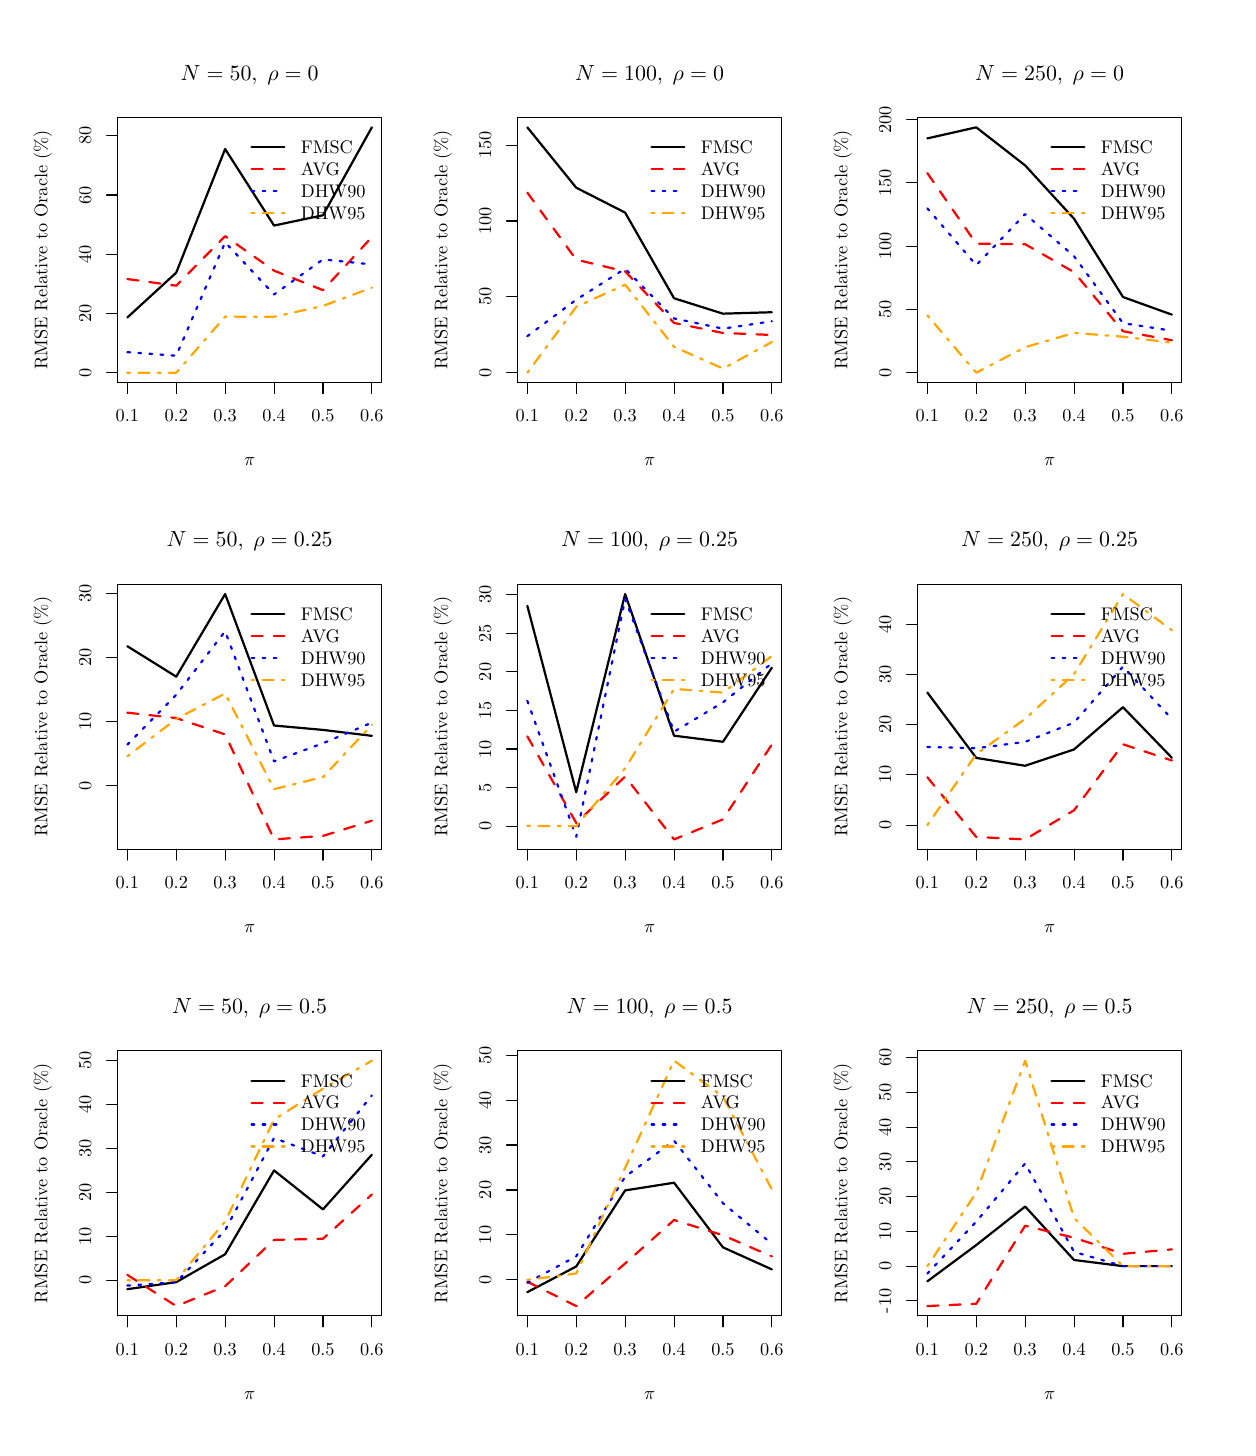
\begin{tikzpicture}[x=1pt,y=1pt]
\definecolor[named]{fillColor}{rgb}{1.00,1.00,1.00}
\path[use as bounding box,fill=fillColor,fill opacity=0.00] (0,0) rectangle (433.62,505.89);
\begin{scope}
\path[clip] ( 32.47,377.65) rectangle (127.91,473.42);
\definecolor[named]{drawColor}{rgb}{0.00,0.00,0.00}

\path[draw=drawColor,line width= 0.8pt,line join=round,line cap=round] ( 36.01,401.15) --
	( 53.68,417.36) --
	( 71.35,462.05) --
	( 89.03,434.38) --
	(106.70,438.10) --
	(124.37,469.87);
\end{scope}
\begin{scope}
\path[clip] (  0.00,  0.00) rectangle (433.62,505.89);
\definecolor[named]{drawColor}{rgb}{0.00,0.00,0.00}

\path[draw=drawColor,line width= 0.4pt,line join=round,line cap=round] ( 36.01,377.65) -- (124.37,377.65);

\path[draw=drawColor,line width= 0.4pt,line join=round,line cap=round] ( 36.01,377.65) -- ( 36.01,373.69);

\path[draw=drawColor,line width= 0.4pt,line join=round,line cap=round] ( 53.68,377.65) -- ( 53.68,373.69);

\path[draw=drawColor,line width= 0.4pt,line join=round,line cap=round] ( 71.35,377.65) -- ( 71.35,373.69);

\path[draw=drawColor,line width= 0.4pt,line join=round,line cap=round] ( 89.03,377.65) -- ( 89.03,373.69);

\path[draw=drawColor,line width= 0.4pt,line join=round,line cap=round] (106.70,377.65) -- (106.70,373.69);

\path[draw=drawColor,line width= 0.4pt,line join=round,line cap=round] (124.37,377.65) -- (124.37,373.69);

\node[text=drawColor,anchor=base,inner sep=0pt, outer sep=0pt, scale=  0.66] at ( 36.01,363.40) {0.1};

\node[text=drawColor,anchor=base,inner sep=0pt, outer sep=0pt, scale=  0.66] at ( 53.68,363.40) {0.2};

\node[text=drawColor,anchor=base,inner sep=0pt, outer sep=0pt, scale=  0.66] at ( 71.35,363.40) {0.3};

\node[text=drawColor,anchor=base,inner sep=0pt, outer sep=0pt, scale=  0.66] at ( 89.03,363.40) {0.4};

\node[text=drawColor,anchor=base,inner sep=0pt, outer sep=0pt, scale=  0.66] at (106.70,363.40) {0.5};

\node[text=drawColor,anchor=base,inner sep=0pt, outer sep=0pt, scale=  0.66] at (124.37,363.40) {0.6};

\path[draw=drawColor,line width= 0.4pt,line join=round,line cap=round] ( 32.47,381.20) -- ( 32.47,466.82);

\path[draw=drawColor,line width= 0.4pt,line join=round,line cap=round] ( 32.47,381.20) -- ( 28.51,381.20);

\path[draw=drawColor,line width= 0.4pt,line join=round,line cap=round] ( 32.47,402.61) -- ( 28.51,402.61);

\path[draw=drawColor,line width= 0.4pt,line join=round,line cap=round] ( 32.47,424.01) -- ( 28.51,424.01);

\path[draw=drawColor,line width= 0.4pt,line join=round,line cap=round] ( 32.47,445.42) -- ( 28.51,445.42);

\path[draw=drawColor,line width= 0.4pt,line join=round,line cap=round] ( 32.47,466.82) -- ( 28.51,466.82);

\node[text=drawColor,rotate= 90.00,anchor=base,inner sep=0pt, outer sep=0pt, scale=  0.66] at ( 22.97,381.20) {0};

\node[text=drawColor,rotate= 90.00,anchor=base,inner sep=0pt, outer sep=0pt, scale=  0.66] at ( 22.97,402.61) {20};

\node[text=drawColor,rotate= 90.00,anchor=base,inner sep=0pt, outer sep=0pt, scale=  0.66] at ( 22.97,424.01) {40};

\node[text=drawColor,rotate= 90.00,anchor=base,inner sep=0pt, outer sep=0pt, scale=  0.66] at ( 22.97,445.42) {60};

\node[text=drawColor,rotate= 90.00,anchor=base,inner sep=0pt, outer sep=0pt, scale=  0.66] at ( 22.97,466.82) {80};

\path[draw=drawColor,line width= 0.4pt,line join=round,line cap=round] ( 32.47,377.65) --
	(127.91,377.65) --
	(127.91,473.42) --
	( 32.47,473.42) --
	( 32.47,377.65);
\end{scope}
\begin{scope}
\path[clip] (  0.00,337.26) rectangle (144.54,505.89);
\definecolor[named]{drawColor}{rgb}{0.00,0.00,0.00}

\node[text=drawColor,anchor=base,inner sep=0pt, outer sep=0pt, scale=  0.79] at ( 80.19,486.92) {\bfseries $N=50, \;\rho=0$};

\node[text=drawColor,anchor=base,inner sep=0pt, outer sep=0pt, scale=  0.66] at ( 80.19,347.56) {$\pi$};

\node[text=drawColor,rotate= 90.00,anchor=base,inner sep=0pt, outer sep=0pt, scale=  0.66] at (  7.13,425.53) {RMSE Relative to Oracle (\%)};
\end{scope}
\begin{scope}
\path[clip] ( 32.47,377.65) rectangle (127.91,473.42);
\definecolor[named]{drawColor}{rgb}{1.00,0.00,0.00}

\path[draw=drawColor,line width= 0.8pt,dash pattern=on 4pt off 4pt ,line join=round,line cap=round] ( 36.01,415.06) --
	( 53.68,412.65) --
	( 71.35,430.56) --
	( 89.03,418.09) --
	(106.70,411.04) --
	(124.37,430.20);
\definecolor[named]{drawColor}{rgb}{0.00,0.00,1.00}

\path[draw=drawColor,line width= 0.8pt,dash pattern=on 1pt off 3pt ,line join=round,line cap=round] ( 36.01,388.64) --
	( 53.68,387.34) --
	( 71.35,428.32) --
	( 89.03,409.47) --
	(106.70,422.15) --
	(124.37,420.33);
\definecolor[named]{drawColor}{rgb}{1.00,0.65,0.00}

\path[draw=drawColor,line width= 0.8pt,dash pattern=on 1pt off 3pt on 4pt off 3pt ,line join=round,line cap=round] ( 36.01,381.20) --
	( 53.68,381.20) --
	( 71.35,401.48) --
	( 89.03,401.42) --
	(106.70,405.34) --
	(124.37,411.94);
\definecolor[named]{drawColor}{rgb}{0.00,0.00,0.00}

\path[draw=drawColor,line width= 0.8pt,line join=round,line cap=round] ( 80.89,462.63) -- ( 92.77,462.63);
\definecolor[named]{drawColor}{rgb}{1.00,0.00,0.00}

\path[draw=drawColor,line width= 0.8pt,dash pattern=on 4pt off 4pt ,line join=round,line cap=round] ( 80.89,454.71) -- ( 92.77,454.71);
\definecolor[named]{drawColor}{rgb}{0.00,0.00,1.00}

\path[draw=drawColor,line width= 0.8pt,dash pattern=on 1pt off 3pt ,line join=round,line cap=round] ( 80.89,446.79) -- ( 92.77,446.79);
\definecolor[named]{drawColor}{rgb}{1.00,0.65,0.00}

\path[draw=drawColor,line width= 0.8pt,dash pattern=on 1pt off 3pt on 4pt off 3pt ,line join=round,line cap=round] ( 80.89,438.87) -- ( 92.77,438.87);
\definecolor[named]{drawColor}{rgb}{0.00,0.00,0.00}

\node[text=drawColor,anchor=base west,inner sep=0pt, outer sep=0pt, scale=  0.66] at ( 98.71,460.35) {FMSC};

\node[text=drawColor,anchor=base west,inner sep=0pt, outer sep=0pt, scale=  0.66] at ( 98.71,452.43) {AVG};

\node[text=drawColor,anchor=base west,inner sep=0pt, outer sep=0pt, scale=  0.66] at ( 98.71,444.51) {DHW90};

\node[text=drawColor,anchor=base west,inner sep=0pt, outer sep=0pt, scale=  0.66] at ( 98.71,436.59) {DHW95};
\end{scope}
\begin{scope}
\path[clip] (177.01,377.65) rectangle (272.45,473.42);
\definecolor[named]{drawColor}{rgb}{0.00,0.00,0.00}

\path[draw=drawColor,line width= 0.8pt,line join=round,line cap=round] (180.55,469.87) --
	(198.22,448.06) --
	(215.89,439.06) --
	(233.57,408.10) --
	(251.24,402.54) --
	(268.91,403.06);
\end{scope}
\begin{scope}
\path[clip] (  0.00,  0.00) rectangle (433.62,505.89);
\definecolor[named]{drawColor}{rgb}{0.00,0.00,0.00}

\path[draw=drawColor,line width= 0.4pt,line join=round,line cap=round] (180.55,377.65) -- (268.91,377.65);

\path[draw=drawColor,line width= 0.4pt,line join=round,line cap=round] (180.55,377.65) -- (180.55,373.69);

\path[draw=drawColor,line width= 0.4pt,line join=round,line cap=round] (198.22,377.65) -- (198.22,373.69);

\path[draw=drawColor,line width= 0.4pt,line join=round,line cap=round] (215.89,377.65) -- (215.89,373.69);

\path[draw=drawColor,line width= 0.4pt,line join=round,line cap=round] (233.57,377.65) -- (233.57,373.69);

\path[draw=drawColor,line width= 0.4pt,line join=round,line cap=round] (251.24,377.65) -- (251.24,373.69);

\path[draw=drawColor,line width= 0.4pt,line join=round,line cap=round] (268.91,377.65) -- (268.91,373.69);

\node[text=drawColor,anchor=base,inner sep=0pt, outer sep=0pt, scale=  0.66] at (180.55,363.40) {0.1};

\node[text=drawColor,anchor=base,inner sep=0pt, outer sep=0pt, scale=  0.66] at (198.22,363.40) {0.2};

\node[text=drawColor,anchor=base,inner sep=0pt, outer sep=0pt, scale=  0.66] at (215.89,363.40) {0.3};

\node[text=drawColor,anchor=base,inner sep=0pt, outer sep=0pt, scale=  0.66] at (233.57,363.40) {0.4};

\node[text=drawColor,anchor=base,inner sep=0pt, outer sep=0pt, scale=  0.66] at (251.24,363.40) {0.5};

\node[text=drawColor,anchor=base,inner sep=0pt, outer sep=0pt, scale=  0.66] at (268.91,363.40) {0.6};

\path[draw=drawColor,line width= 0.4pt,line join=round,line cap=round] (177.01,381.20) -- (177.01,463.45);

\path[draw=drawColor,line width= 0.4pt,line join=round,line cap=round] (177.01,381.20) -- (173.05,381.20);

\path[draw=drawColor,line width= 0.4pt,line join=round,line cap=round] (177.01,408.62) -- (173.05,408.62);

\path[draw=drawColor,line width= 0.4pt,line join=round,line cap=round] (177.01,436.03) -- (173.05,436.03);

\path[draw=drawColor,line width= 0.4pt,line join=round,line cap=round] (177.01,463.45) -- (173.05,463.45);

\node[text=drawColor,rotate= 90.00,anchor=base,inner sep=0pt, outer sep=0pt, scale=  0.66] at (167.51,381.20) {0};

\node[text=drawColor,rotate= 90.00,anchor=base,inner sep=0pt, outer sep=0pt, scale=  0.66] at (167.51,408.62) {50};

\node[text=drawColor,rotate= 90.00,anchor=base,inner sep=0pt, outer sep=0pt, scale=  0.66] at (167.51,436.03) {100};

\node[text=drawColor,rotate= 90.00,anchor=base,inner sep=0pt, outer sep=0pt, scale=  0.66] at (167.51,463.45) {150};

\path[draw=drawColor,line width= 0.4pt,line join=round,line cap=round] (177.01,377.65) --
	(272.45,377.65) --
	(272.45,473.42) --
	(177.01,473.42) --
	(177.01,377.65);
\end{scope}
\begin{scope}
\path[clip] (144.54,337.26) rectangle (289.08,505.89);
\definecolor[named]{drawColor}{rgb}{0.00,0.00,0.00}

\node[text=drawColor,anchor=base,inner sep=0pt, outer sep=0pt, scale=  0.79] at (224.73,486.92) {\bfseries $N=100, \;\rho=0$};

\node[text=drawColor,anchor=base,inner sep=0pt, outer sep=0pt, scale=  0.66] at (224.73,347.56) {$\pi$};

\node[text=drawColor,rotate= 90.00,anchor=base,inner sep=0pt, outer sep=0pt, scale=  0.66] at (151.67,425.53) {RMSE Relative to Oracle (\%)};
\end{scope}
\begin{scope}
\path[clip] (177.01,377.65) rectangle (272.45,473.42);
\definecolor[named]{drawColor}{rgb}{1.00,0.00,0.00}

\path[draw=drawColor,line width= 0.8pt,dash pattern=on 4pt off 4pt ,line join=round,line cap=round] (180.55,446.28) --
	(198.22,422.06) --
	(215.89,417.81) --
	(233.57,399.19) --
	(251.24,395.57) --
	(268.91,394.84);
\definecolor[named]{drawColor}{rgb}{0.00,0.00,1.00}

\path[draw=drawColor,line width= 0.8pt,dash pattern=on 1pt off 3pt ,line join=round,line cap=round] (180.55,394.41) --
	(198.22,407.60) --
	(215.89,418.80) --
	(233.57,400.82) --
	(251.24,397.12) --
	(268.91,399.80);
\definecolor[named]{drawColor}{rgb}{1.00,0.65,0.00}

\path[draw=drawColor,line width= 0.8pt,dash pattern=on 1pt off 3pt on 4pt off 3pt ,line join=round,line cap=round] (180.55,381.20) --
	(198.22,405.02) --
	(215.89,413.03) --
	(233.57,390.56) --
	(251.24,382.69) --
	(268.91,392.30);
\definecolor[named]{drawColor}{rgb}{0.00,0.00,0.00}

\path[draw=drawColor,line width= 0.8pt,line join=round,line cap=round] (225.43,462.63) -- (237.31,462.63);
\definecolor[named]{drawColor}{rgb}{1.00,0.00,0.00}

\path[draw=drawColor,line width= 0.8pt,dash pattern=on 4pt off 4pt ,line join=round,line cap=round] (225.43,454.71) -- (237.31,454.71);
\definecolor[named]{drawColor}{rgb}{0.00,0.00,1.00}

\path[draw=drawColor,line width= 0.8pt,dash pattern=on 1pt off 3pt ,line join=round,line cap=round] (225.43,446.79) -- (237.31,446.79);
\definecolor[named]{drawColor}{rgb}{1.00,0.65,0.00}

\path[draw=drawColor,line width= 0.8pt,dash pattern=on 1pt off 3pt on 4pt off 3pt ,line join=round,line cap=round] (225.43,438.87) -- (237.31,438.87);
\definecolor[named]{drawColor}{rgb}{0.00,0.00,0.00}

\node[text=drawColor,anchor=base west,inner sep=0pt, outer sep=0pt, scale=  0.66] at (243.25,460.35) {FMSC};

\node[text=drawColor,anchor=base west,inner sep=0pt, outer sep=0pt, scale=  0.66] at (243.25,452.43) {AVG};

\node[text=drawColor,anchor=base west,inner sep=0pt, outer sep=0pt, scale=  0.66] at (243.25,444.51) {DHW90};

\node[text=drawColor,anchor=base west,inner sep=0pt, outer sep=0pt, scale=  0.66] at (243.25,436.59) {DHW95};
\end{scope}
\begin{scope}
\path[clip] (321.55,377.65) rectangle (416.99,473.42);
\definecolor[named]{drawColor}{rgb}{0.00,0.00,0.00}

\path[draw=drawColor,line width= 0.8pt,line join=round,line cap=round] (325.09,465.87) --
	(342.76,469.87) --
	(360.43,456.11) --
	(378.11,436.82) --
	(395.78,408.56) --
	(413.45,402.19);
\end{scope}
\begin{scope}
\path[clip] (  0.00,  0.00) rectangle (433.62,505.89);
\definecolor[named]{drawColor}{rgb}{0.00,0.00,0.00}

\path[draw=drawColor,line width= 0.4pt,line join=round,line cap=round] (325.09,377.65) -- (413.45,377.65);

\path[draw=drawColor,line width= 0.4pt,line join=round,line cap=round] (325.09,377.65) -- (325.09,373.69);

\path[draw=drawColor,line width= 0.4pt,line join=round,line cap=round] (342.76,377.65) -- (342.76,373.69);

\path[draw=drawColor,line width= 0.4pt,line join=round,line cap=round] (360.43,377.65) -- (360.43,373.69);

\path[draw=drawColor,line width= 0.4pt,line join=round,line cap=round] (378.11,377.65) -- (378.11,373.69);

\path[draw=drawColor,line width= 0.4pt,line join=round,line cap=round] (395.78,377.65) -- (395.78,373.69);

\path[draw=drawColor,line width= 0.4pt,line join=round,line cap=round] (413.45,377.65) -- (413.45,373.69);

\node[text=drawColor,anchor=base,inner sep=0pt, outer sep=0pt, scale=  0.66] at (325.09,363.40) {0.1};

\node[text=drawColor,anchor=base,inner sep=0pt, outer sep=0pt, scale=  0.66] at (342.76,363.40) {0.2};

\node[text=drawColor,anchor=base,inner sep=0pt, outer sep=0pt, scale=  0.66] at (360.43,363.40) {0.3};

\node[text=drawColor,anchor=base,inner sep=0pt, outer sep=0pt, scale=  0.66] at (378.11,363.40) {0.4};

\node[text=drawColor,anchor=base,inner sep=0pt, outer sep=0pt, scale=  0.66] at (395.78,363.40) {0.5};

\node[text=drawColor,anchor=base,inner sep=0pt, outer sep=0pt, scale=  0.66] at (413.45,363.40) {0.6};

\path[draw=drawColor,line width= 0.4pt,line join=round,line cap=round] (321.55,381.20) -- (321.55,472.67);

\path[draw=drawColor,line width= 0.4pt,line join=round,line cap=round] (321.55,381.20) -- (317.59,381.20);

\path[draw=drawColor,line width= 0.4pt,line join=round,line cap=round] (321.55,404.07) -- (317.59,404.07);

\path[draw=drawColor,line width= 0.4pt,line join=round,line cap=round] (321.55,426.94) -- (317.59,426.94);

\path[draw=drawColor,line width= 0.4pt,line join=round,line cap=round] (321.55,449.80) -- (317.59,449.80);

\path[draw=drawColor,line width= 0.4pt,line join=round,line cap=round] (321.55,472.67) -- (317.59,472.67);

\node[text=drawColor,rotate= 90.00,anchor=base,inner sep=0pt, outer sep=0pt, scale=  0.66] at (312.05,381.20) {0};

\node[text=drawColor,rotate= 90.00,anchor=base,inner sep=0pt, outer sep=0pt, scale=  0.66] at (312.05,404.07) {50};

\node[text=drawColor,rotate= 90.00,anchor=base,inner sep=0pt, outer sep=0pt, scale=  0.66] at (312.05,426.94) {100};

\node[text=drawColor,rotate= 90.00,anchor=base,inner sep=0pt, outer sep=0pt, scale=  0.66] at (312.05,449.80) {150};

\node[text=drawColor,rotate= 90.00,anchor=base,inner sep=0pt, outer sep=0pt, scale=  0.66] at (312.05,472.67) {200};

\path[draw=drawColor,line width= 0.4pt,line join=round,line cap=round] (321.55,377.65) --
	(416.99,377.65) --
	(416.99,473.42) --
	(321.55,473.42) --
	(321.55,377.65);
\end{scope}
\begin{scope}
\path[clip] (289.08,337.26) rectangle (433.62,505.89);
\definecolor[named]{drawColor}{rgb}{0.00,0.00,0.00}

\node[text=drawColor,anchor=base,inner sep=0pt, outer sep=0pt, scale=  0.79] at (369.27,486.92) {\bfseries $N=250, \;\rho=0$};

\node[text=drawColor,anchor=base,inner sep=0pt, outer sep=0pt, scale=  0.66] at (369.27,347.56) {$\pi$};

\node[text=drawColor,rotate= 90.00,anchor=base,inner sep=0pt, outer sep=0pt, scale=  0.66] at (296.21,425.53) {RMSE Relative to Oracle (\%)};
\end{scope}
\begin{scope}
\path[clip] (321.55,377.65) rectangle (416.99,473.42);
\definecolor[named]{drawColor}{rgb}{1.00,0.00,0.00}

\path[draw=drawColor,line width= 0.8pt,dash pattern=on 4pt off 4pt ,line join=round,line cap=round] (325.09,453.34) --
	(342.76,427.84) --
	(360.43,427.65) --
	(378.11,417.53) --
	(395.78,396.20) --
	(413.45,392.93);
\definecolor[named]{drawColor}{rgb}{0.00,0.00,1.00}

\path[draw=drawColor,line width= 0.8pt,dash pattern=on 1pt off 3pt ,line join=round,line cap=round] (325.09,440.61) --
	(342.76,420.05) --
	(360.43,438.52) --
	(378.11,423.30) --
	(395.78,399.11) --
	(413.45,396.38);
\definecolor[named]{drawColor}{rgb}{1.00,0.65,0.00}

\path[draw=drawColor,line width= 0.8pt,dash pattern=on 1pt off 3pt on 4pt off 3pt ,line join=round,line cap=round] (325.09,401.95) --
	(342.76,381.20) --
	(360.43,390.42) --
	(378.11,395.59) --
	(395.78,394.21) --
	(413.45,392.07);
\definecolor[named]{drawColor}{rgb}{0.00,0.00,0.00}

\path[draw=drawColor,line width= 0.8pt,line join=round,line cap=round] (369.97,462.63) -- (381.85,462.63);
\definecolor[named]{drawColor}{rgb}{1.00,0.00,0.00}

\path[draw=drawColor,line width= 0.8pt,dash pattern=on 4pt off 4pt ,line join=round,line cap=round] (369.97,454.71) -- (381.85,454.71);
\definecolor[named]{drawColor}{rgb}{0.00,0.00,1.00}

\path[draw=drawColor,line width= 0.8pt,dash pattern=on 1pt off 3pt ,line join=round,line cap=round] (369.97,446.79) -- (381.85,446.79);
\definecolor[named]{drawColor}{rgb}{1.00,0.65,0.00}

\path[draw=drawColor,line width= 0.8pt,dash pattern=on 1pt off 3pt on 4pt off 3pt ,line join=round,line cap=round] (369.97,438.87) -- (381.85,438.87);
\definecolor[named]{drawColor}{rgb}{0.00,0.00,0.00}

\node[text=drawColor,anchor=base west,inner sep=0pt, outer sep=0pt, scale=  0.66] at (387.79,460.35) {FMSC};

\node[text=drawColor,anchor=base west,inner sep=0pt, outer sep=0pt, scale=  0.66] at (387.79,452.43) {AVG};

\node[text=drawColor,anchor=base west,inner sep=0pt, outer sep=0pt, scale=  0.66] at (387.79,444.51) {DHW90};

\node[text=drawColor,anchor=base west,inner sep=0pt, outer sep=0pt, scale=  0.66] at (387.79,436.59) {DHW95};
\end{scope}
\begin{scope}
\path[clip] ( 32.47,209.02) rectangle (127.91,304.79);
\definecolor[named]{drawColor}{rgb}{0.00,0.00,0.00}

\path[draw=drawColor,line width= 0.8pt,line join=round,line cap=round] ( 36.01,282.38) --
	( 53.68,271.37) --
	( 71.35,301.24) --
	( 89.03,253.72) --
	(106.70,252.13) --
	(124.37,249.99);
\end{scope}
\begin{scope}
\path[clip] (  0.00,  0.00) rectangle (433.62,505.89);
\definecolor[named]{drawColor}{rgb}{0.00,0.00,0.00}

\path[draw=drawColor,line width= 0.4pt,line join=round,line cap=round] ( 36.01,209.02) -- (124.37,209.02);

\path[draw=drawColor,line width= 0.4pt,line join=round,line cap=round] ( 36.01,209.02) -- ( 36.01,205.06);

\path[draw=drawColor,line width= 0.4pt,line join=round,line cap=round] ( 53.68,209.02) -- ( 53.68,205.06);

\path[draw=drawColor,line width= 0.4pt,line join=round,line cap=round] ( 71.35,209.02) -- ( 71.35,205.06);

\path[draw=drawColor,line width= 0.4pt,line join=round,line cap=round] ( 89.03,209.02) -- ( 89.03,205.06);

\path[draw=drawColor,line width= 0.4pt,line join=round,line cap=round] (106.70,209.02) -- (106.70,205.06);

\path[draw=drawColor,line width= 0.4pt,line join=round,line cap=round] (124.37,209.02) -- (124.37,205.06);

\node[text=drawColor,anchor=base,inner sep=0pt, outer sep=0pt, scale=  0.66] at ( 36.01,194.77) {0.1};

\node[text=drawColor,anchor=base,inner sep=0pt, outer sep=0pt, scale=  0.66] at ( 53.68,194.77) {0.2};

\node[text=drawColor,anchor=base,inner sep=0pt, outer sep=0pt, scale=  0.66] at ( 71.35,194.77) {0.3};

\node[text=drawColor,anchor=base,inner sep=0pt, outer sep=0pt, scale=  0.66] at ( 89.03,194.77) {0.4};

\node[text=drawColor,anchor=base,inner sep=0pt, outer sep=0pt, scale=  0.66] at (106.70,194.77) {0.5};

\node[text=drawColor,anchor=base,inner sep=0pt, outer sep=0pt, scale=  0.66] at (124.37,194.77) {0.6};

\path[draw=drawColor,line width= 0.4pt,line join=round,line cap=round] ( 32.47,231.90) -- ( 32.47,301.58);

\path[draw=drawColor,line width= 0.4pt,line join=round,line cap=round] ( 32.47,231.90) -- ( 28.51,231.90);

\path[draw=drawColor,line width= 0.4pt,line join=round,line cap=round] ( 32.47,255.13) -- ( 28.51,255.13);

\path[draw=drawColor,line width= 0.4pt,line join=round,line cap=round] ( 32.47,278.35) -- ( 28.51,278.35);

\path[draw=drawColor,line width= 0.4pt,line join=round,line cap=round] ( 32.47,301.58) -- ( 28.51,301.58);

\node[text=drawColor,rotate= 90.00,anchor=base,inner sep=0pt, outer sep=0pt, scale=  0.66] at ( 22.97,231.90) {0};

\node[text=drawColor,rotate= 90.00,anchor=base,inner sep=0pt, outer sep=0pt, scale=  0.66] at ( 22.97,255.13) {10};

\node[text=drawColor,rotate= 90.00,anchor=base,inner sep=0pt, outer sep=0pt, scale=  0.66] at ( 22.97,278.35) {20};

\node[text=drawColor,rotate= 90.00,anchor=base,inner sep=0pt, outer sep=0pt, scale=  0.66] at ( 22.97,301.58) {30};

\path[draw=drawColor,line width= 0.4pt,line join=round,line cap=round] ( 32.47,209.02) --
	(127.91,209.02) --
	(127.91,304.79) --
	( 32.47,304.79) --
	( 32.47,209.02);
\end{scope}
\begin{scope}
\path[clip] (  0.00,168.63) rectangle (144.54,337.26);
\definecolor[named]{drawColor}{rgb}{0.00,0.00,0.00}

\node[text=drawColor,anchor=base,inner sep=0pt, outer sep=0pt, scale=  0.79] at ( 80.19,318.29) {\bfseries $N=50, \;\rho=0.25$};

\node[text=drawColor,anchor=base,inner sep=0pt, outer sep=0pt, scale=  0.66] at ( 80.19,178.93) {$\pi$};

\node[text=drawColor,rotate= 90.00,anchor=base,inner sep=0pt, outer sep=0pt, scale=  0.66] at (  7.13,256.90) {RMSE Relative to Oracle (\%)};
\end{scope}
\begin{scope}
\path[clip] ( 32.47,209.02) rectangle (127.91,304.79);
\definecolor[named]{drawColor}{rgb}{1.00,0.00,0.00}

\path[draw=drawColor,line width= 0.8pt,dash pattern=on 4pt off 4pt ,line join=round,line cap=round] ( 36.01,258.36) --
	( 53.68,256.41) --
	( 71.35,250.51) --
	( 89.03,212.57) --
	(106.70,213.83) --
	(124.37,219.33);
\definecolor[named]{drawColor}{rgb}{0.00,0.00,1.00}

\path[draw=drawColor,line width= 0.8pt,dash pattern=on 1pt off 3pt ,line join=round,line cap=round] ( 36.01,246.81) --
	( 53.68,264.82) --
	( 71.35,287.77) --
	( 89.03,240.78) --
	(106.70,247.31) --
	(124.37,254.76);
\definecolor[named]{drawColor}{rgb}{1.00,0.65,0.00}

\path[draw=drawColor,line width= 0.8pt,dash pattern=on 1pt off 3pt on 4pt off 3pt ,line join=round,line cap=round] ( 36.01,242.60) --
	( 53.68,256.07) --
	( 71.35,265.30) --
	( 89.03,230.73) --
	(106.70,235.10) --
	(124.37,253.92);
\definecolor[named]{drawColor}{rgb}{0.00,0.00,0.00}

\path[draw=drawColor,line width= 0.8pt,line join=round,line cap=round] ( 80.89,294.00) -- ( 92.77,294.00);
\definecolor[named]{drawColor}{rgb}{1.00,0.00,0.00}

\path[draw=drawColor,line width= 0.8pt,dash pattern=on 4pt off 4pt ,line join=round,line cap=round] ( 80.89,286.08) -- ( 92.77,286.08);
\definecolor[named]{drawColor}{rgb}{0.00,0.00,1.00}

\path[draw=drawColor,line width= 0.8pt,dash pattern=on 1pt off 3pt ,line join=round,line cap=round] ( 80.89,278.16) -- ( 92.77,278.16);
\definecolor[named]{drawColor}{rgb}{1.00,0.65,0.00}

\path[draw=drawColor,line width= 0.8pt,dash pattern=on 1pt off 3pt on 4pt off 3pt ,line join=round,line cap=round] ( 80.89,270.24) -- ( 92.77,270.24);
\definecolor[named]{drawColor}{rgb}{0.00,0.00,0.00}

\node[text=drawColor,anchor=base west,inner sep=0pt, outer sep=0pt, scale=  0.66] at ( 98.71,291.72) {FMSC};

\node[text=drawColor,anchor=base west,inner sep=0pt, outer sep=0pt, scale=  0.66] at ( 98.71,283.80) {AVG};

\node[text=drawColor,anchor=base west,inner sep=0pt, outer sep=0pt, scale=  0.66] at ( 98.71,275.88) {DHW90};

\node[text=drawColor,anchor=base west,inner sep=0pt, outer sep=0pt, scale=  0.66] at ( 98.71,267.96) {DHW95};
\end{scope}
\begin{scope}
\path[clip] (177.01,209.02) rectangle (272.45,304.79);
\definecolor[named]{drawColor}{rgb}{0.00,0.00,0.00}

\path[draw=drawColor,line width= 0.8pt,line join=round,line cap=round] (180.55,296.96) --
	(198.22,229.64) --
	(215.89,301.24) --
	(233.57,250.04) --
	(251.24,247.84) --
	(268.91,274.62);
\end{scope}
\begin{scope}
\path[clip] (  0.00,  0.00) rectangle (433.62,505.89);
\definecolor[named]{drawColor}{rgb}{0.00,0.00,0.00}

\path[draw=drawColor,line width= 0.4pt,line join=round,line cap=round] (180.55,209.02) -- (268.91,209.02);

\path[draw=drawColor,line width= 0.4pt,line join=round,line cap=round] (180.55,209.02) -- (180.55,205.06);

\path[draw=drawColor,line width= 0.4pt,line join=round,line cap=round] (198.22,209.02) -- (198.22,205.06);

\path[draw=drawColor,line width= 0.4pt,line join=round,line cap=round] (215.89,209.02) -- (215.89,205.06);

\path[draw=drawColor,line width= 0.4pt,line join=round,line cap=round] (233.57,209.02) -- (233.57,205.06);

\path[draw=drawColor,line width= 0.4pt,line join=round,line cap=round] (251.24,209.02) -- (251.24,205.06);

\path[draw=drawColor,line width= 0.4pt,line join=round,line cap=round] (268.91,209.02) -- (268.91,205.06);

\node[text=drawColor,anchor=base,inner sep=0pt, outer sep=0pt, scale=  0.66] at (180.55,194.77) {0.1};

\node[text=drawColor,anchor=base,inner sep=0pt, outer sep=0pt, scale=  0.66] at (198.22,194.77) {0.2};

\node[text=drawColor,anchor=base,inner sep=0pt, outer sep=0pt, scale=  0.66] at (215.89,194.77) {0.3};

\node[text=drawColor,anchor=base,inner sep=0pt, outer sep=0pt, scale=  0.66] at (233.57,194.77) {0.4};

\node[text=drawColor,anchor=base,inner sep=0pt, outer sep=0pt, scale=  0.66] at (251.24,194.77) {0.5};

\node[text=drawColor,anchor=base,inner sep=0pt, outer sep=0pt, scale=  0.66] at (268.91,194.77) {0.6};

\path[draw=drawColor,line width= 0.4pt,line join=round,line cap=round] (177.01,217.34) -- (177.01,300.98);

\path[draw=drawColor,line width= 0.4pt,line join=round,line cap=round] (177.01,217.34) -- (173.05,217.34);

\path[draw=drawColor,line width= 0.4pt,line join=round,line cap=round] (177.01,231.28) -- (173.05,231.28);

\path[draw=drawColor,line width= 0.4pt,line join=round,line cap=round] (177.01,245.22) -- (173.05,245.22);

\path[draw=drawColor,line width= 0.4pt,line join=round,line cap=round] (177.01,259.16) -- (173.05,259.16);

\path[draw=drawColor,line width= 0.4pt,line join=round,line cap=round] (177.01,273.10) -- (173.05,273.10);

\path[draw=drawColor,line width= 0.4pt,line join=round,line cap=round] (177.01,287.04) -- (173.05,287.04);

\path[draw=drawColor,line width= 0.4pt,line join=round,line cap=round] (177.01,300.98) -- (173.05,300.98);

\node[text=drawColor,rotate= 90.00,anchor=base,inner sep=0pt, outer sep=0pt, scale=  0.66] at (167.51,217.34) {0};

\node[text=drawColor,rotate= 90.00,anchor=base,inner sep=0pt, outer sep=0pt, scale=  0.66] at (167.51,231.28) {5};

\node[text=drawColor,rotate= 90.00,anchor=base,inner sep=0pt, outer sep=0pt, scale=  0.66] at (167.51,245.22) {10};

\node[text=drawColor,rotate= 90.00,anchor=base,inner sep=0pt, outer sep=0pt, scale=  0.66] at (167.51,259.16) {15};

\node[text=drawColor,rotate= 90.00,anchor=base,inner sep=0pt, outer sep=0pt, scale=  0.66] at (167.51,273.10) {20};

\node[text=drawColor,rotate= 90.00,anchor=base,inner sep=0pt, outer sep=0pt, scale=  0.66] at (167.51,287.04) {25};

\node[text=drawColor,rotate= 90.00,anchor=base,inner sep=0pt, outer sep=0pt, scale=  0.66] at (167.51,300.98) {30};

\path[draw=drawColor,line width= 0.4pt,line join=round,line cap=round] (177.01,209.02) --
	(272.45,209.02) --
	(272.45,304.79) --
	(177.01,304.79) --
	(177.01,209.02);
\end{scope}
\begin{scope}
\path[clip] (144.54,168.63) rectangle (289.08,337.26);
\definecolor[named]{drawColor}{rgb}{0.00,0.00,0.00}

\node[text=drawColor,anchor=base,inner sep=0pt, outer sep=0pt, scale=  0.79] at (224.73,318.29) {\bfseries $N=100, \;\rho=0.25$};

\node[text=drawColor,anchor=base,inner sep=0pt, outer sep=0pt, scale=  0.66] at (224.73,178.93) {$\pi$};

\node[text=drawColor,rotate= 90.00,anchor=base,inner sep=0pt, outer sep=0pt, scale=  0.66] at (151.67,256.90) {RMSE Relative to Oracle (\%)};
\end{scope}
\begin{scope}
\path[clip] (177.01,209.02) rectangle (272.45,304.79);
\definecolor[named]{drawColor}{rgb}{1.00,0.00,0.00}

\path[draw=drawColor,line width= 0.8pt,dash pattern=on 4pt off 4pt ,line join=round,line cap=round] (180.55,249.81) --
	(198.22,218.53) --
	(215.89,235.27) --
	(233.57,212.57) --
	(251.24,219.81) --
	(268.91,246.87);
\definecolor[named]{drawColor}{rgb}{0.00,0.00,1.00}

\path[draw=drawColor,line width= 0.8pt,dash pattern=on 1pt off 3pt ,line join=round,line cap=round] (180.55,262.65) --
	(198.22,213.53) --
	(215.89,299.54) --
	(233.57,251.48) --
	(251.24,262.09) --
	(268.91,276.21);
\definecolor[named]{drawColor}{rgb}{1.00,0.65,0.00}

\path[draw=drawColor,line width= 0.8pt,dash pattern=on 1pt off 3pt on 4pt off 3pt ,line join=round,line cap=round] (180.55,217.48) --
	(198.22,217.35) --
	(215.89,238.28) --
	(233.57,266.96) --
	(251.24,265.63) --
	(268.91,278.85);
\definecolor[named]{drawColor}{rgb}{0.00,0.00,0.00}

\path[draw=drawColor,line width= 0.8pt,line join=round,line cap=round] (225.43,294.00) -- (237.31,294.00);
\definecolor[named]{drawColor}{rgb}{1.00,0.00,0.00}

\path[draw=drawColor,line width= 0.8pt,dash pattern=on 4pt off 4pt ,line join=round,line cap=round] (225.43,286.08) -- (237.31,286.08);
\definecolor[named]{drawColor}{rgb}{0.00,0.00,1.00}

\path[draw=drawColor,line width= 0.8pt,dash pattern=on 1pt off 3pt ,line join=round,line cap=round] (225.43,278.16) -- (237.31,278.16);
\definecolor[named]{drawColor}{rgb}{1.00,0.65,0.00}

\path[draw=drawColor,line width= 0.8pt,dash pattern=on 1pt off 3pt on 4pt off 3pt ,line join=round,line cap=round] (225.43,270.24) -- (237.31,270.24);
\definecolor[named]{drawColor}{rgb}{0.00,0.00,0.00}

\node[text=drawColor,anchor=base west,inner sep=0pt, outer sep=0pt, scale=  0.66] at (243.25,291.72) {FMSC};

\node[text=drawColor,anchor=base west,inner sep=0pt, outer sep=0pt, scale=  0.66] at (243.25,283.80) {AVG};

\node[text=drawColor,anchor=base west,inner sep=0pt, outer sep=0pt, scale=  0.66] at (243.25,275.88) {DHW90};

\node[text=drawColor,anchor=base west,inner sep=0pt, outer sep=0pt, scale=  0.66] at (243.25,267.96) {DHW95};
\end{scope}
\begin{scope}
\path[clip] (321.55,209.02) rectangle (416.99,304.79);
\definecolor[named]{drawColor}{rgb}{0.00,0.00,0.00}

\path[draw=drawColor,line width= 0.8pt,line join=round,line cap=round] (325.09,265.65) --
	(342.76,242.02) --
	(360.43,239.17) --
	(378.11,245.09) --
	(395.78,260.33) --
	(413.45,242.07);
\end{scope}
\begin{scope}
\path[clip] (  0.00,  0.00) rectangle (433.62,505.89);
\definecolor[named]{drawColor}{rgb}{0.00,0.00,0.00}

\path[draw=drawColor,line width= 0.4pt,line join=round,line cap=round] (325.09,209.02) -- (413.45,209.02);

\path[draw=drawColor,line width= 0.4pt,line join=round,line cap=round] (325.09,209.02) -- (325.09,205.06);

\path[draw=drawColor,line width= 0.4pt,line join=round,line cap=round] (342.76,209.02) -- (342.76,205.06);

\path[draw=drawColor,line width= 0.4pt,line join=round,line cap=round] (360.43,209.02) -- (360.43,205.06);

\path[draw=drawColor,line width= 0.4pt,line join=round,line cap=round] (378.11,209.02) -- (378.11,205.06);

\path[draw=drawColor,line width= 0.4pt,line join=round,line cap=round] (395.78,209.02) -- (395.78,205.06);

\path[draw=drawColor,line width= 0.4pt,line join=round,line cap=round] (413.45,209.02) -- (413.45,205.06);

\node[text=drawColor,anchor=base,inner sep=0pt, outer sep=0pt, scale=  0.66] at (325.09,194.77) {0.1};

\node[text=drawColor,anchor=base,inner sep=0pt, outer sep=0pt, scale=  0.66] at (342.76,194.77) {0.2};

\node[text=drawColor,anchor=base,inner sep=0pt, outer sep=0pt, scale=  0.66] at (360.43,194.77) {0.3};

\node[text=drawColor,anchor=base,inner sep=0pt, outer sep=0pt, scale=  0.66] at (378.11,194.77) {0.4};

\node[text=drawColor,anchor=base,inner sep=0pt, outer sep=0pt, scale=  0.66] at (395.78,194.77) {0.5};

\node[text=drawColor,anchor=base,inner sep=0pt, outer sep=0pt, scale=  0.66] at (413.45,194.77) {0.6};

\path[draw=drawColor,line width= 0.4pt,line join=round,line cap=round] (321.55,217.74) -- (321.55,290.37);

\path[draw=drawColor,line width= 0.4pt,line join=round,line cap=round] (321.55,217.74) -- (317.59,217.74);

\path[draw=drawColor,line width= 0.4pt,line join=round,line cap=round] (321.55,235.90) -- (317.59,235.90);

\path[draw=drawColor,line width= 0.4pt,line join=round,line cap=round] (321.55,254.06) -- (317.59,254.06);

\path[draw=drawColor,line width= 0.4pt,line join=round,line cap=round] (321.55,272.21) -- (317.59,272.21);

\path[draw=drawColor,line width= 0.4pt,line join=round,line cap=round] (321.55,290.37) -- (317.59,290.37);

\node[text=drawColor,rotate= 90.00,anchor=base,inner sep=0pt, outer sep=0pt, scale=  0.66] at (312.05,217.74) {0};

\node[text=drawColor,rotate= 90.00,anchor=base,inner sep=0pt, outer sep=0pt, scale=  0.66] at (312.05,235.90) {10};

\node[text=drawColor,rotate= 90.00,anchor=base,inner sep=0pt, outer sep=0pt, scale=  0.66] at (312.05,254.06) {20};

\node[text=drawColor,rotate= 90.00,anchor=base,inner sep=0pt, outer sep=0pt, scale=  0.66] at (312.05,272.21) {30};

\node[text=drawColor,rotate= 90.00,anchor=base,inner sep=0pt, outer sep=0pt, scale=  0.66] at (312.05,290.37) {40};

\path[draw=drawColor,line width= 0.4pt,line join=round,line cap=round] (321.55,209.02) --
	(416.99,209.02) --
	(416.99,304.79) --
	(321.55,304.79) --
	(321.55,209.02);
\end{scope}
\begin{scope}
\path[clip] (289.08,168.63) rectangle (433.62,337.26);
\definecolor[named]{drawColor}{rgb}{0.00,0.00,0.00}

\node[text=drawColor,anchor=base,inner sep=0pt, outer sep=0pt, scale=  0.79] at (369.27,318.29) {\bfseries $N=250, \;\rho=0.25$};

\node[text=drawColor,anchor=base,inner sep=0pt, outer sep=0pt, scale=  0.66] at (369.27,178.93) {$\pi$};

\node[text=drawColor,rotate= 90.00,anchor=base,inner sep=0pt, outer sep=0pt, scale=  0.66] at (296.21,256.90) {RMSE Relative to Oracle (\%)};
\end{scope}
\begin{scope}
\path[clip] (321.55,209.02) rectangle (416.99,304.79);
\definecolor[named]{drawColor}{rgb}{1.00,0.00,0.00}

\path[draw=drawColor,line width= 0.8pt,dash pattern=on 4pt off 4pt ,line join=round,line cap=round] (325.09,235.04) --
	(342.76,213.45) --
	(360.43,212.57) --
	(378.11,223.11) --
	(395.78,246.94) --
	(413.45,241.09);
\definecolor[named]{drawColor}{rgb}{0.00,0.00,1.00}

\path[draw=drawColor,line width= 0.8pt,dash pattern=on 1pt off 3pt ,line join=round,line cap=round] (325.09,245.98) --
	(342.76,245.50) --
	(360.43,247.81) --
	(378.11,254.77) --
	(395.78,275.00) --
	(413.45,256.10);
\definecolor[named]{drawColor}{rgb}{1.00,0.65,0.00}

\path[draw=drawColor,line width= 0.8pt,dash pattern=on 1pt off 3pt on 4pt off 3pt ,line join=round,line cap=round] (325.09,217.74) --
	(342.76,243.38) --
	(360.43,256.13) --
	(378.11,272.27) --
	(395.78,301.24) --
	(413.45,288.16);
\definecolor[named]{drawColor}{rgb}{0.00,0.00,0.00}

\path[draw=drawColor,line width= 0.8pt,line join=round,line cap=round] (369.97,294.00) -- (381.85,294.00);
\definecolor[named]{drawColor}{rgb}{1.00,0.00,0.00}

\path[draw=drawColor,line width= 0.8pt,dash pattern=on 4pt off 4pt ,line join=round,line cap=round] (369.97,286.08) -- (381.85,286.08);
\definecolor[named]{drawColor}{rgb}{0.00,0.00,1.00}

\path[draw=drawColor,line width= 0.8pt,dash pattern=on 1pt off 3pt ,line join=round,line cap=round] (369.97,278.16) -- (381.85,278.16);
\definecolor[named]{drawColor}{rgb}{1.00,0.65,0.00}

\path[draw=drawColor,line width= 0.8pt,dash pattern=on 1pt off 3pt on 4pt off 3pt ,line join=round,line cap=round] (369.97,270.24) -- (381.85,270.24);
\definecolor[named]{drawColor}{rgb}{0.00,0.00,0.00}

\node[text=drawColor,anchor=base west,inner sep=0pt, outer sep=0pt, scale=  0.66] at (387.79,291.72) {FMSC};

\node[text=drawColor,anchor=base west,inner sep=0pt, outer sep=0pt, scale=  0.66] at (387.79,283.80) {AVG};

\node[text=drawColor,anchor=base west,inner sep=0pt, outer sep=0pt, scale=  0.66] at (387.79,275.88) {DHW90};

\node[text=drawColor,anchor=base west,inner sep=0pt, outer sep=0pt, scale=  0.66] at (387.79,267.96) {DHW95};
\end{scope}
\begin{scope}
\path[clip] ( 32.47, 40.39) rectangle (127.91,136.16);
\definecolor[named]{drawColor}{rgb}{0.00,0.00,0.00}

\path[draw=drawColor,line width= 0.8pt,line join=round,line cap=round] ( 36.01, 50.04) --
	( 53.68, 52.59) --
	( 71.35, 62.66) --
	( 89.03, 92.96) --
	(106.70, 78.87) --
	(124.37, 98.63);
\end{scope}
\begin{scope}
\path[clip] (  0.00,  0.00) rectangle (433.62,505.89);
\definecolor[named]{drawColor}{rgb}{0.00,0.00,0.00}

\path[draw=drawColor,line width= 0.4pt,line join=round,line cap=round] ( 36.01, 40.39) -- (124.37, 40.39);

\path[draw=drawColor,line width= 0.4pt,line join=round,line cap=round] ( 36.01, 40.39) -- ( 36.01, 36.43);

\path[draw=drawColor,line width= 0.4pt,line join=round,line cap=round] ( 53.68, 40.39) -- ( 53.68, 36.43);

\path[draw=drawColor,line width= 0.4pt,line join=round,line cap=round] ( 71.35, 40.39) -- ( 71.35, 36.43);

\path[draw=drawColor,line width= 0.4pt,line join=round,line cap=round] ( 89.03, 40.39) -- ( 89.03, 36.43);

\path[draw=drawColor,line width= 0.4pt,line join=round,line cap=round] (106.70, 40.39) -- (106.70, 36.43);

\path[draw=drawColor,line width= 0.4pt,line join=round,line cap=round] (124.37, 40.39) -- (124.37, 36.43);

\node[text=drawColor,anchor=base,inner sep=0pt, outer sep=0pt, scale=  0.66] at ( 36.01, 26.14) {0.1};

\node[text=drawColor,anchor=base,inner sep=0pt, outer sep=0pt, scale=  0.66] at ( 53.68, 26.14) {0.2};

\node[text=drawColor,anchor=base,inner sep=0pt, outer sep=0pt, scale=  0.66] at ( 71.35, 26.14) {0.3};

\node[text=drawColor,anchor=base,inner sep=0pt, outer sep=0pt, scale=  0.66] at ( 89.03, 26.14) {0.4};

\node[text=drawColor,anchor=base,inner sep=0pt, outer sep=0pt, scale=  0.66] at (106.70, 26.14) {0.5};

\node[text=drawColor,anchor=base,inner sep=0pt, outer sep=0pt, scale=  0.66] at (124.37, 26.14) {0.6};

\path[draw=drawColor,line width= 0.4pt,line join=round,line cap=round] ( 32.47, 53.26) -- ( 32.47,132.65);

\path[draw=drawColor,line width= 0.4pt,line join=round,line cap=round] ( 32.47, 53.26) -- ( 28.51, 53.26);

\path[draw=drawColor,line width= 0.4pt,line join=round,line cap=round] ( 32.47, 69.14) -- ( 28.51, 69.14);

\path[draw=drawColor,line width= 0.4pt,line join=round,line cap=round] ( 32.47, 85.02) -- ( 28.51, 85.02);

\path[draw=drawColor,line width= 0.4pt,line join=round,line cap=round] ( 32.47,100.90) -- ( 28.51,100.90);

\path[draw=drawColor,line width= 0.4pt,line join=round,line cap=round] ( 32.47,116.77) -- ( 28.51,116.77);

\path[draw=drawColor,line width= 0.4pt,line join=round,line cap=round] ( 32.47,132.65) -- ( 28.51,132.65);

\node[text=drawColor,rotate= 90.00,anchor=base,inner sep=0pt, outer sep=0pt, scale=  0.66] at ( 22.97, 53.26) {0};

\node[text=drawColor,rotate= 90.00,anchor=base,inner sep=0pt, outer sep=0pt, scale=  0.66] at ( 22.97, 69.14) {10};

\node[text=drawColor,rotate= 90.00,anchor=base,inner sep=0pt, outer sep=0pt, scale=  0.66] at ( 22.97, 85.02) {20};

\node[text=drawColor,rotate= 90.00,anchor=base,inner sep=0pt, outer sep=0pt, scale=  0.66] at ( 22.97,100.90) {30};

\node[text=drawColor,rotate= 90.00,anchor=base,inner sep=0pt, outer sep=0pt, scale=  0.66] at ( 22.97,116.77) {40};

\node[text=drawColor,rotate= 90.00,anchor=base,inner sep=0pt, outer sep=0pt, scale=  0.66] at ( 22.97,132.65) {50};

\path[draw=drawColor,line width= 0.4pt,line join=round,line cap=round] ( 32.47, 40.39) --
	(127.91, 40.39) --
	(127.91,136.16) --
	( 32.47,136.16) --
	( 32.47, 40.39);
\end{scope}
\begin{scope}
\path[clip] (  0.00,  0.00) rectangle (144.54,168.63);
\definecolor[named]{drawColor}{rgb}{0.00,0.00,0.00}

\node[text=drawColor,anchor=base,inner sep=0pt, outer sep=0pt, scale=  0.79] at ( 80.19,149.66) {\bfseries $N=50, \;\rho=0.5$};

\node[text=drawColor,anchor=base,inner sep=0pt, outer sep=0pt, scale=  0.66] at ( 80.19, 10.30) {$\pi$};

\node[text=drawColor,rotate= 90.00,anchor=base,inner sep=0pt, outer sep=0pt, scale=  0.66] at (  7.13, 88.27) {RMSE Relative to Oracle (\%)};
\end{scope}
\begin{scope}
\path[clip] ( 32.47, 40.39) rectangle (127.91,136.16);
\definecolor[named]{drawColor}{rgb}{1.00,0.00,0.00}

\path[draw=drawColor,line width= 0.8pt,dash pattern=on 4pt off 4pt ,line join=round,line cap=round] ( 36.01, 55.21) --
	( 53.68, 43.94) --
	( 71.35, 51.11) --
	( 89.03, 67.85) --
	(106.70, 68.26) --
	(124.37, 84.26);
\definecolor[named]{drawColor}{rgb}{0.00,0.00,1.00}

\path[draw=drawColor,line width= 0.8pt,dash pattern=on 1pt off 3pt ,line join=round,line cap=round] ( 36.01, 51.35) --
	( 53.68, 52.54) --
	( 71.35, 71.33) --
	( 89.03,104.69) --
	(106.70, 98.03) --
	(124.37,120.07);
\definecolor[named]{drawColor}{rgb}{1.00,0.65,0.00}

\path[draw=drawColor,line width= 0.8pt,dash pattern=on 1pt off 3pt on 4pt off 3pt ,line join=round,line cap=round] ( 36.01, 53.26) --
	( 53.68, 53.26) --
	( 71.35, 74.51) --
	( 89.03,111.36) --
	(106.70,122.48) --
	(124.37,132.61);
\definecolor[named]{drawColor}{rgb}{0.00,0.00,0.00}

\path[draw=drawColor,line width= 0.8pt,line join=round,line cap=round] ( 80.89,125.37) -- ( 92.77,125.37);
\definecolor[named]{drawColor}{rgb}{1.00,0.00,0.00}

\path[draw=drawColor,line width= 0.8pt,dash pattern=on 4pt off 4pt ,line join=round,line cap=round] ( 80.89,117.45) -- ( 92.77,117.45);
\definecolor[named]{drawColor}{rgb}{0.00,0.00,1.00}

\path[draw=drawColor,line width= 0.8pt,dash pattern=on 1pt off 3pt ,line join=round,line cap=round] ( 80.89,109.53) -- ( 92.77,109.53);
\definecolor[named]{drawColor}{rgb}{1.00,0.65,0.00}

\path[draw=drawColor,line width= 0.8pt,dash pattern=on 1pt off 3pt on 4pt off 3pt ,line join=round,line cap=round] ( 80.89,101.61) -- ( 92.77,101.61);
\definecolor[named]{drawColor}{rgb}{0.00,0.00,0.00}

\node[text=drawColor,anchor=base west,inner sep=0pt, outer sep=0pt, scale=  0.66] at ( 98.71,123.09) {FMSC};

\node[text=drawColor,anchor=base west,inner sep=0pt, outer sep=0pt, scale=  0.66] at ( 98.71,115.17) {AVG};

\node[text=drawColor,anchor=base west,inner sep=0pt, outer sep=0pt, scale=  0.66] at ( 98.71,107.25) {DHW90};

\node[text=drawColor,anchor=base west,inner sep=0pt, outer sep=0pt, scale=  0.66] at ( 98.71, 99.33) {DHW95};
\end{scope}
\begin{scope}
\path[clip] (177.01, 40.39) rectangle (272.45,136.16);
\definecolor[named]{drawColor}{rgb}{0.00,0.00,0.00}

\path[draw=drawColor,line width= 0.8pt,line join=round,line cap=round] (180.55, 48.97) --
	(198.22, 58.25) --
	(215.89, 85.73) --
	(233.57, 88.51) --
	(251.24, 65.16) --
	(268.91, 57.19);
\end{scope}
\begin{scope}
\path[clip] (  0.00,  0.00) rectangle (433.62,505.89);
\definecolor[named]{drawColor}{rgb}{0.00,0.00,0.00}

\path[draw=drawColor,line width= 0.4pt,line join=round,line cap=round] (180.55, 40.39) -- (268.91, 40.39);

\path[draw=drawColor,line width= 0.4pt,line join=round,line cap=round] (180.55, 40.39) -- (180.55, 36.43);

\path[draw=drawColor,line width= 0.4pt,line join=round,line cap=round] (198.22, 40.39) -- (198.22, 36.43);

\path[draw=drawColor,line width= 0.4pt,line join=round,line cap=round] (215.89, 40.39) -- (215.89, 36.43);

\path[draw=drawColor,line width= 0.4pt,line join=round,line cap=round] (233.57, 40.39) -- (233.57, 36.43);

\path[draw=drawColor,line width= 0.4pt,line join=round,line cap=round] (251.24, 40.39) -- (251.24, 36.43);

\path[draw=drawColor,line width= 0.4pt,line join=round,line cap=round] (268.91, 40.39) -- (268.91, 36.43);

\node[text=drawColor,anchor=base,inner sep=0pt, outer sep=0pt, scale=  0.66] at (180.55, 26.14) {0.1};

\node[text=drawColor,anchor=base,inner sep=0pt, outer sep=0pt, scale=  0.66] at (198.22, 26.14) {0.2};

\node[text=drawColor,anchor=base,inner sep=0pt, outer sep=0pt, scale=  0.66] at (215.89, 26.14) {0.3};

\node[text=drawColor,anchor=base,inner sep=0pt, outer sep=0pt, scale=  0.66] at (233.57, 26.14) {0.4};

\node[text=drawColor,anchor=base,inner sep=0pt, outer sep=0pt, scale=  0.66] at (251.24, 26.14) {0.5};

\node[text=drawColor,anchor=base,inner sep=0pt, outer sep=0pt, scale=  0.66] at (268.91, 26.14) {0.6};

\path[draw=drawColor,line width= 0.4pt,line join=round,line cap=round] (177.01, 53.41) -- (177.01,134.62);

\path[draw=drawColor,line width= 0.4pt,line join=round,line cap=round] (177.01, 53.41) -- (173.05, 53.41);

\path[draw=drawColor,line width= 0.4pt,line join=round,line cap=round] (177.01, 69.66) -- (173.05, 69.66);

\path[draw=drawColor,line width= 0.4pt,line join=round,line cap=round] (177.01, 85.90) -- (173.05, 85.90);

\path[draw=drawColor,line width= 0.4pt,line join=round,line cap=round] (177.01,102.14) -- (173.05,102.14);

\path[draw=drawColor,line width= 0.4pt,line join=round,line cap=round] (177.01,118.38) -- (173.05,118.38);

\path[draw=drawColor,line width= 0.4pt,line join=round,line cap=round] (177.01,134.62) -- (173.05,134.62);

\node[text=drawColor,rotate= 90.00,anchor=base,inner sep=0pt, outer sep=0pt, scale=  0.66] at (167.51, 53.41) {0};

\node[text=drawColor,rotate= 90.00,anchor=base,inner sep=0pt, outer sep=0pt, scale=  0.66] at (167.51, 69.66) {10};

\node[text=drawColor,rotate= 90.00,anchor=base,inner sep=0pt, outer sep=0pt, scale=  0.66] at (167.51, 85.90) {20};

\node[text=drawColor,rotate= 90.00,anchor=base,inner sep=0pt, outer sep=0pt, scale=  0.66] at (167.51,102.14) {30};

\node[text=drawColor,rotate= 90.00,anchor=base,inner sep=0pt, outer sep=0pt, scale=  0.66] at (167.51,118.38) {40};

\node[text=drawColor,rotate= 90.00,anchor=base,inner sep=0pt, outer sep=0pt, scale=  0.66] at (167.51,134.62) {50};

\path[draw=drawColor,line width= 0.4pt,line join=round,line cap=round] (177.01, 40.39) --
	(272.45, 40.39) --
	(272.45,136.16) --
	(177.01,136.16) --
	(177.01, 40.39);
\end{scope}
\begin{scope}
\path[clip] (144.54,  0.00) rectangle (289.08,168.63);
\definecolor[named]{drawColor}{rgb}{0.00,0.00,0.00}

\node[text=drawColor,anchor=base,inner sep=0pt, outer sep=0pt, scale=  0.79] at (224.73,149.66) {\bfseries $N=100, \;\rho=0.5$};

\node[text=drawColor,anchor=base,inner sep=0pt, outer sep=0pt, scale=  0.66] at (224.73, 10.30) {$\pi$};

\node[text=drawColor,rotate= 90.00,anchor=base,inner sep=0pt, outer sep=0pt, scale=  0.66] at (151.67, 88.27) {RMSE Relative to Oracle (\%)};
\end{scope}
\begin{scope}
\path[clip] (177.01, 40.39) rectangle (272.45,136.16);
\definecolor[named]{drawColor}{rgb}{1.00,0.00,0.00}

\path[draw=drawColor,line width= 0.8pt,dash pattern=on 4pt off 4pt ,line join=round,line cap=round] (180.55, 52.75) --
	(198.22, 43.94) --
	(215.89, 59.34) --
	(233.57, 75.04) --
	(251.24, 69.52) --
	(268.91, 61.86);
\definecolor[named]{drawColor}{rgb}{0.00,0.00,1.00}

\path[draw=drawColor,line width= 0.8pt,dash pattern=on 1pt off 3pt ,line join=round,line cap=round] (180.55, 52.35) --
	(198.22, 61.92) --
	(215.89, 90.70) --
	(233.57,103.70) --
	(251.24, 81.11) --
	(268.91, 66.43);
\definecolor[named]{drawColor}{rgb}{1.00,0.65,0.00}

\path[draw=drawColor,line width= 0.8pt,dash pattern=on 1pt off 3pt on 4pt off 3pt ,line join=round,line cap=round] (180.55, 53.41) --
	(198.22, 55.71) --
	(215.89, 93.91) --
	(233.57,132.61) --
	(251.24,119.62) --
	(268.91, 86.09);
\definecolor[named]{drawColor}{rgb}{0.00,0.00,0.00}

\path[draw=drawColor,line width= 0.8pt,line join=round,line cap=round] (225.43,125.37) -- (237.31,125.37);
\definecolor[named]{drawColor}{rgb}{1.00,0.00,0.00}

\path[draw=drawColor,line width= 0.8pt,dash pattern=on 4pt off 4pt ,line join=round,line cap=round] (225.43,117.45) -- (237.31,117.45);
\definecolor[named]{drawColor}{rgb}{0.00,0.00,1.00}

\path[draw=drawColor,line width= 0.8pt,dash pattern=on 1pt off 3pt ,line join=round,line cap=round] (225.43,109.53) -- (237.31,109.53);
\definecolor[named]{drawColor}{rgb}{1.00,0.65,0.00}

\path[draw=drawColor,line width= 0.8pt,dash pattern=on 1pt off 3pt on 4pt off 3pt ,line join=round,line cap=round] (225.43,101.61) -- (237.31,101.61);
\definecolor[named]{drawColor}{rgb}{0.00,0.00,0.00}

\node[text=drawColor,anchor=base west,inner sep=0pt, outer sep=0pt, scale=  0.66] at (243.25,123.09) {FMSC};

\node[text=drawColor,anchor=base west,inner sep=0pt, outer sep=0pt, scale=  0.66] at (243.25,115.17) {AVG};

\node[text=drawColor,anchor=base west,inner sep=0pt, outer sep=0pt, scale=  0.66] at (243.25,107.25) {DHW90};

\node[text=drawColor,anchor=base west,inner sep=0pt, outer sep=0pt, scale=  0.66] at (243.25, 99.33) {DHW95};
\end{scope}
\begin{scope}
\path[clip] (321.55, 40.39) rectangle (416.99,136.16);
\definecolor[named]{drawColor}{rgb}{0.00,0.00,0.00}

\path[draw=drawColor,line width= 0.8pt,line join=round,line cap=round] (325.09, 52.87) --
	(342.76, 65.98) --
	(360.43, 79.90) --
	(378.11, 60.60) --
	(395.78, 58.37) --
	(413.45, 58.37);
\end{scope}
\begin{scope}
\path[clip] (  0.00,  0.00) rectangle (433.62,505.89);
\definecolor[named]{drawColor}{rgb}{0.00,0.00,0.00}

\path[draw=drawColor,line width= 0.4pt,line join=round,line cap=round] (325.09, 40.39) -- (413.45, 40.39);

\path[draw=drawColor,line width= 0.4pt,line join=round,line cap=round] (325.09, 40.39) -- (325.09, 36.43);

\path[draw=drawColor,line width= 0.4pt,line join=round,line cap=round] (342.76, 40.39) -- (342.76, 36.43);

\path[draw=drawColor,line width= 0.4pt,line join=round,line cap=round] (360.43, 40.39) -- (360.43, 36.43);

\path[draw=drawColor,line width= 0.4pt,line join=round,line cap=round] (378.11, 40.39) -- (378.11, 36.43);

\path[draw=drawColor,line width= 0.4pt,line join=round,line cap=round] (395.78, 40.39) -- (395.78, 36.43);

\path[draw=drawColor,line width= 0.4pt,line join=round,line cap=round] (413.45, 40.39) -- (413.45, 36.43);

\node[text=drawColor,anchor=base,inner sep=0pt, outer sep=0pt, scale=  0.66] at (325.09, 26.14) {0.1};

\node[text=drawColor,anchor=base,inner sep=0pt, outer sep=0pt, scale=  0.66] at (342.76, 26.14) {0.2};

\node[text=drawColor,anchor=base,inner sep=0pt, outer sep=0pt, scale=  0.66] at (360.43, 26.14) {0.3};

\node[text=drawColor,anchor=base,inner sep=0pt, outer sep=0pt, scale=  0.66] at (378.11, 26.14) {0.4};

\node[text=drawColor,anchor=base,inner sep=0pt, outer sep=0pt, scale=  0.66] at (395.78, 26.14) {0.5};

\node[text=drawColor,anchor=base,inner sep=0pt, outer sep=0pt, scale=  0.66] at (413.45, 26.14) {0.6};

\path[draw=drawColor,line width= 0.4pt,line join=round,line cap=round] (321.55, 45.81) -- (321.55,133.67);

\path[draw=drawColor,line width= 0.4pt,line join=round,line cap=round] (321.55, 45.81) -- (317.59, 45.81);

\path[draw=drawColor,line width= 0.4pt,line join=round,line cap=round] (321.55, 58.37) -- (317.59, 58.37);

\path[draw=drawColor,line width= 0.4pt,line join=round,line cap=round] (321.55, 70.92) -- (317.59, 70.92);

\path[draw=drawColor,line width= 0.4pt,line join=round,line cap=round] (321.55, 83.47) -- (317.59, 83.47);

\path[draw=drawColor,line width= 0.4pt,line join=round,line cap=round] (321.55, 96.02) -- (317.59, 96.02);

\path[draw=drawColor,line width= 0.4pt,line join=round,line cap=round] (321.55,108.57) -- (317.59,108.57);

\path[draw=drawColor,line width= 0.4pt,line join=round,line cap=round] (321.55,121.12) -- (317.59,121.12);

\path[draw=drawColor,line width= 0.4pt,line join=round,line cap=round] (321.55,133.67) -- (317.59,133.67);

\node[text=drawColor,rotate= 90.00,anchor=base,inner sep=0pt, outer sep=0pt, scale=  0.66] at (312.05, 45.81) {-10};

\node[text=drawColor,rotate= 90.00,anchor=base,inner sep=0pt, outer sep=0pt, scale=  0.66] at (312.05, 58.37) {0};

\node[text=drawColor,rotate= 90.00,anchor=base,inner sep=0pt, outer sep=0pt, scale=  0.66] at (312.05, 70.92) {10};

\node[text=drawColor,rotate= 90.00,anchor=base,inner sep=0pt, outer sep=0pt, scale=  0.66] at (312.05, 83.47) {20};

\node[text=drawColor,rotate= 90.00,anchor=base,inner sep=0pt, outer sep=0pt, scale=  0.66] at (312.05, 96.02) {30};

\node[text=drawColor,rotate= 90.00,anchor=base,inner sep=0pt, outer sep=0pt, scale=  0.66] at (312.05,108.57) {40};

\node[text=drawColor,rotate= 90.00,anchor=base,inner sep=0pt, outer sep=0pt, scale=  0.66] at (312.05,121.12) {50};

\node[text=drawColor,rotate= 90.00,anchor=base,inner sep=0pt, outer sep=0pt, scale=  0.66] at (312.05,133.67) {60};

\path[draw=drawColor,line width= 0.4pt,line join=round,line cap=round] (321.55, 40.39) --
	(416.99, 40.39) --
	(416.99,136.16) --
	(321.55,136.16) --
	(321.55, 40.39);
\end{scope}
\begin{scope}
\path[clip] (289.08,  0.00) rectangle (433.62,168.63);
\definecolor[named]{drawColor}{rgb}{0.00,0.00,0.00}

\node[text=drawColor,anchor=base,inner sep=0pt, outer sep=0pt, scale=  0.79] at (369.27,149.66) {\bfseries $N=250, \;\rho=0.5$};

\node[text=drawColor,anchor=base,inner sep=0pt, outer sep=0pt, scale=  0.66] at (369.27, 10.30) {$\pi$};

\node[text=drawColor,rotate= 90.00,anchor=base,inner sep=0pt, outer sep=0pt, scale=  0.66] at (296.21, 88.27) {RMSE Relative to Oracle (\%)};
\end{scope}
\begin{scope}
\path[clip] (321.55, 40.39) rectangle (416.99,136.16);
\definecolor[named]{drawColor}{rgb}{1.00,0.00,0.00}

\path[draw=drawColor,line width= 0.8pt,dash pattern=on 4pt off 4pt ,line join=round,line cap=round] (325.09, 43.94) --
	(342.76, 44.77) --
	(360.43, 72.97) --
	(378.11, 68.63) --
	(395.78, 62.82) --
	(413.45, 64.44);
\definecolor[named]{drawColor}{rgb}{0.00,0.00,1.00}

\path[draw=drawColor,line width= 0.8pt,dash pattern=on 1pt off 3pt ,line join=round,line cap=round] (325.09, 55.67) --
	(342.76, 74.45) --
	(360.43, 95.46) --
	(378.11, 63.53) --
	(395.78, 58.37) --
	(413.45, 58.37);
\definecolor[named]{drawColor}{rgb}{1.00,0.65,0.00}

\path[draw=drawColor,line width= 0.8pt,dash pattern=on 1pt off 3pt on 4pt off 3pt ,line join=round,line cap=round] (325.09, 58.37) --
	(342.76, 84.89) --
	(360.43,132.61) --
	(378.11, 75.78) --
	(395.78, 58.37) --
	(413.45, 58.37);
\definecolor[named]{drawColor}{rgb}{0.00,0.00,0.00}

\path[draw=drawColor,line width= 0.8pt,line join=round,line cap=round] (369.97,125.37) -- (381.85,125.37);
\definecolor[named]{drawColor}{rgb}{1.00,0.00,0.00}

\path[draw=drawColor,line width= 0.8pt,dash pattern=on 4pt off 4pt ,line join=round,line cap=round] (369.97,117.45) -- (381.85,117.45);
\definecolor[named]{drawColor}{rgb}{0.00,0.00,1.00}

\path[draw=drawColor,line width= 0.8pt,dash pattern=on 1pt off 3pt ,line join=round,line cap=round] (369.97,109.53) -- (381.85,109.53);
\definecolor[named]{drawColor}{rgb}{1.00,0.65,0.00}

\path[draw=drawColor,line width= 0.8pt,dash pattern=on 1pt off 3pt on 4pt off 3pt ,line join=round,line cap=round] (369.97,101.61) -- (381.85,101.61);
\definecolor[named]{drawColor}{rgb}{0.00,0.00,0.00}

\node[text=drawColor,anchor=base west,inner sep=0pt, outer sep=0pt, scale=  0.66] at (387.79,123.09) {FMSC};

\node[text=drawColor,anchor=base west,inner sep=0pt, outer sep=0pt, scale=  0.66] at (387.79,115.17) {AVG};

\node[text=drawColor,anchor=base west,inner sep=0pt, outer sep=0pt, scale=  0.66] at (387.79,107.25) {DHW90};

\node[text=drawColor,anchor=base west,inner sep=0pt, outer sep=0pt, scale=  0.66] at (387.79, 99.33) {DHW95};
\end{scope}
\end{tikzpicture}

	\caption{OLS vs IV simulation.}
\end{figure}

\begin{figure}
\centering
	% Created by tikzDevice version 0.7.0 on 2014-06-29 19:22:43
% !TEX encoding = UTF-8 Unicode
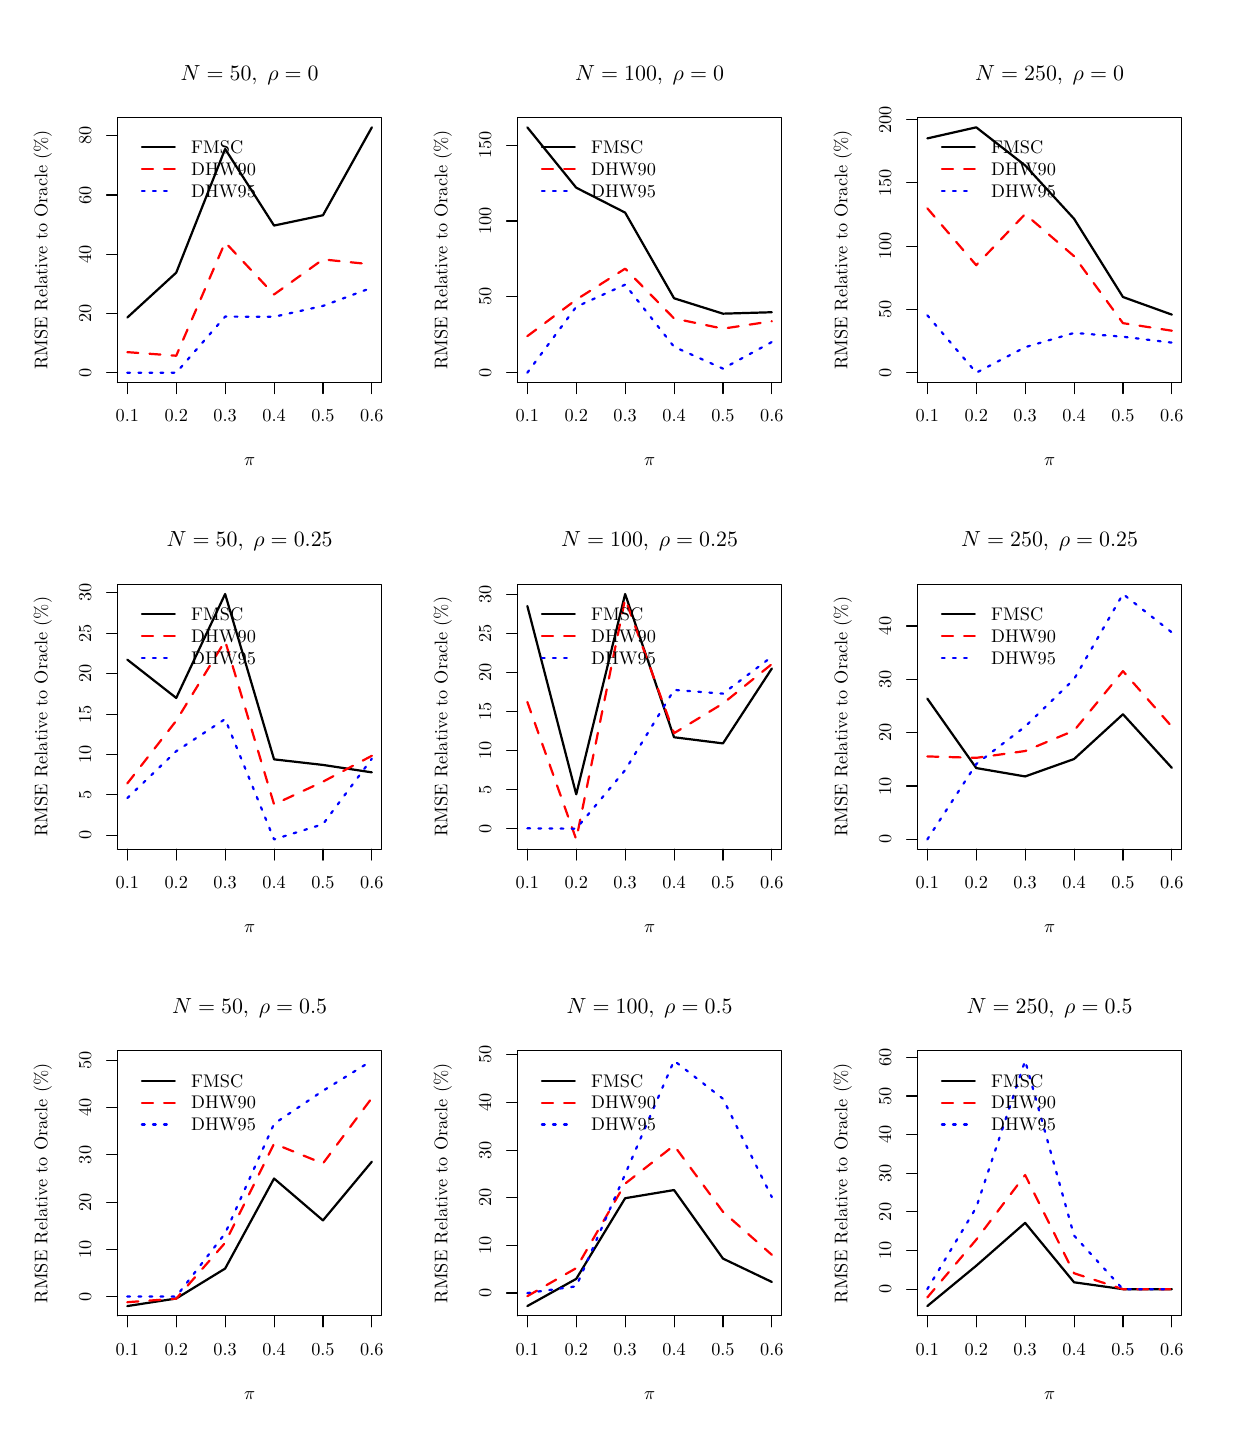
\begin{tikzpicture}[x=1pt,y=1pt]
\definecolor[named]{fillColor}{rgb}{1.00,1.00,1.00}
\path[use as bounding box,fill=fillColor,fill opacity=0.00] (0,0) rectangle (433.62,505.89);
\begin{scope}
\path[clip] ( 32.47,377.65) rectangle (127.91,473.42);
\definecolor[named]{drawColor}{rgb}{0.00,0.00,0.00}

\path[draw=drawColor,line width= 0.8pt,line join=round,line cap=round] ( 36.01,401.15) --
	( 53.68,417.36) --
	( 71.35,462.05) --
	( 89.03,434.38) --
	(106.70,438.10) --
	(124.37,469.87);
\end{scope}
\begin{scope}
\path[clip] (  0.00,  0.00) rectangle (433.62,505.89);
\definecolor[named]{drawColor}{rgb}{0.00,0.00,0.00}

\path[draw=drawColor,line width= 0.4pt,line join=round,line cap=round] ( 36.01,377.65) -- (124.37,377.65);

\path[draw=drawColor,line width= 0.4pt,line join=round,line cap=round] ( 36.01,377.65) -- ( 36.01,373.69);

\path[draw=drawColor,line width= 0.4pt,line join=round,line cap=round] ( 53.68,377.65) -- ( 53.68,373.69);

\path[draw=drawColor,line width= 0.4pt,line join=round,line cap=round] ( 71.35,377.65) -- ( 71.35,373.69);

\path[draw=drawColor,line width= 0.4pt,line join=round,line cap=round] ( 89.03,377.65) -- ( 89.03,373.69);

\path[draw=drawColor,line width= 0.4pt,line join=round,line cap=round] (106.70,377.65) -- (106.70,373.69);

\path[draw=drawColor,line width= 0.4pt,line join=round,line cap=round] (124.37,377.65) -- (124.37,373.69);

\node[text=drawColor,anchor=base,inner sep=0pt, outer sep=0pt, scale=  0.66] at ( 36.01,363.40) {0.1};

\node[text=drawColor,anchor=base,inner sep=0pt, outer sep=0pt, scale=  0.66] at ( 53.68,363.40) {0.2};

\node[text=drawColor,anchor=base,inner sep=0pt, outer sep=0pt, scale=  0.66] at ( 71.35,363.40) {0.3};

\node[text=drawColor,anchor=base,inner sep=0pt, outer sep=0pt, scale=  0.66] at ( 89.03,363.40) {0.4};

\node[text=drawColor,anchor=base,inner sep=0pt, outer sep=0pt, scale=  0.66] at (106.70,363.40) {0.5};

\node[text=drawColor,anchor=base,inner sep=0pt, outer sep=0pt, scale=  0.66] at (124.37,363.40) {0.6};

\path[draw=drawColor,line width= 0.4pt,line join=round,line cap=round] ( 32.47,381.20) -- ( 32.47,466.82);

\path[draw=drawColor,line width= 0.4pt,line join=round,line cap=round] ( 32.47,381.20) -- ( 28.51,381.20);

\path[draw=drawColor,line width= 0.4pt,line join=round,line cap=round] ( 32.47,402.61) -- ( 28.51,402.61);

\path[draw=drawColor,line width= 0.4pt,line join=round,line cap=round] ( 32.47,424.01) -- ( 28.51,424.01);

\path[draw=drawColor,line width= 0.4pt,line join=round,line cap=round] ( 32.47,445.42) -- ( 28.51,445.42);

\path[draw=drawColor,line width= 0.4pt,line join=round,line cap=round] ( 32.47,466.82) -- ( 28.51,466.82);

\node[text=drawColor,rotate= 90.00,anchor=base,inner sep=0pt, outer sep=0pt, scale=  0.66] at ( 22.97,381.20) {0};

\node[text=drawColor,rotate= 90.00,anchor=base,inner sep=0pt, outer sep=0pt, scale=  0.66] at ( 22.97,402.61) {20};

\node[text=drawColor,rotate= 90.00,anchor=base,inner sep=0pt, outer sep=0pt, scale=  0.66] at ( 22.97,424.01) {40};

\node[text=drawColor,rotate= 90.00,anchor=base,inner sep=0pt, outer sep=0pt, scale=  0.66] at ( 22.97,445.42) {60};

\node[text=drawColor,rotate= 90.00,anchor=base,inner sep=0pt, outer sep=0pt, scale=  0.66] at ( 22.97,466.82) {80};

\path[draw=drawColor,line width= 0.4pt,line join=round,line cap=round] ( 32.47,377.65) --
	(127.91,377.65) --
	(127.91,473.42) --
	( 32.47,473.42) --
	( 32.47,377.65);
\end{scope}
\begin{scope}
\path[clip] (  0.00,337.26) rectangle (144.54,505.89);
\definecolor[named]{drawColor}{rgb}{0.00,0.00,0.00}

\node[text=drawColor,anchor=base,inner sep=0pt, outer sep=0pt, scale=  0.79] at ( 80.19,486.92) {\bfseries $N=50, \;\rho=0$};

\node[text=drawColor,anchor=base,inner sep=0pt, outer sep=0pt, scale=  0.66] at ( 80.19,347.56) {$\pi$};

\node[text=drawColor,rotate= 90.00,anchor=base,inner sep=0pt, outer sep=0pt, scale=  0.66] at (  7.13,425.53) {RMSE Relative to Oracle (\%)};
\end{scope}
\begin{scope}
\path[clip] ( 32.47,377.65) rectangle (127.91,473.42);
\definecolor[named]{drawColor}{rgb}{1.00,0.00,0.00}

\path[draw=drawColor,line width= 0.8pt,dash pattern=on 4pt off 4pt ,line join=round,line cap=round] ( 36.01,388.64) --
	( 53.68,387.34) --
	( 71.35,428.32) --
	( 89.03,409.47) --
	(106.70,422.15) --
	(124.37,420.33);
\definecolor[named]{drawColor}{rgb}{0.00,0.00,1.00}

\path[draw=drawColor,line width= 0.8pt,dash pattern=on 1pt off 3pt ,line join=round,line cap=round] ( 36.01,381.20) --
	( 53.68,381.20) --
	( 71.35,401.48) --
	( 89.03,401.42) --
	(106.70,405.34) --
	(124.37,411.94);
\definecolor[named]{drawColor}{rgb}{0.00,0.00,0.00}

\path[draw=drawColor,line width= 0.8pt,line join=round,line cap=round] ( 41.28,462.63) -- ( 53.16,462.63);
\definecolor[named]{drawColor}{rgb}{1.00,0.00,0.00}

\path[draw=drawColor,line width= 0.8pt,dash pattern=on 4pt off 4pt ,line join=round,line cap=round] ( 41.28,454.71) -- ( 53.16,454.71);
\definecolor[named]{drawColor}{rgb}{0.00,0.00,1.00}

\path[draw=drawColor,line width= 0.8pt,dash pattern=on 1pt off 3pt ,line join=round,line cap=round] ( 41.28,446.79) -- ( 53.16,446.79);
\definecolor[named]{drawColor}{rgb}{0.00,0.00,0.00}

\node[text=drawColor,anchor=base west,inner sep=0pt, outer sep=0pt, scale=  0.66] at ( 59.10,460.35) {FMSC};

\node[text=drawColor,anchor=base west,inner sep=0pt, outer sep=0pt, scale=  0.66] at ( 59.10,452.43) {DHW90};

\node[text=drawColor,anchor=base west,inner sep=0pt, outer sep=0pt, scale=  0.66] at ( 59.10,444.51) {DHW95};
\end{scope}
\begin{scope}
\path[clip] (177.01,377.65) rectangle (272.45,473.42);
\definecolor[named]{drawColor}{rgb}{0.00,0.00,0.00}

\path[draw=drawColor,line width= 0.8pt,line join=round,line cap=round] (180.55,469.87) --
	(198.22,448.06) --
	(215.89,439.06) --
	(233.57,408.10) --
	(251.24,402.54) --
	(268.91,403.06);
\end{scope}
\begin{scope}
\path[clip] (  0.00,  0.00) rectangle (433.62,505.89);
\definecolor[named]{drawColor}{rgb}{0.00,0.00,0.00}

\path[draw=drawColor,line width= 0.4pt,line join=round,line cap=round] (180.55,377.65) -- (268.91,377.65);

\path[draw=drawColor,line width= 0.4pt,line join=round,line cap=round] (180.55,377.65) -- (180.55,373.69);

\path[draw=drawColor,line width= 0.4pt,line join=round,line cap=round] (198.22,377.65) -- (198.22,373.69);

\path[draw=drawColor,line width= 0.4pt,line join=round,line cap=round] (215.89,377.65) -- (215.89,373.69);

\path[draw=drawColor,line width= 0.4pt,line join=round,line cap=round] (233.57,377.65) -- (233.57,373.69);

\path[draw=drawColor,line width= 0.4pt,line join=round,line cap=round] (251.24,377.65) -- (251.24,373.69);

\path[draw=drawColor,line width= 0.4pt,line join=round,line cap=round] (268.91,377.65) -- (268.91,373.69);

\node[text=drawColor,anchor=base,inner sep=0pt, outer sep=0pt, scale=  0.66] at (180.55,363.40) {0.1};

\node[text=drawColor,anchor=base,inner sep=0pt, outer sep=0pt, scale=  0.66] at (198.22,363.40) {0.2};

\node[text=drawColor,anchor=base,inner sep=0pt, outer sep=0pt, scale=  0.66] at (215.89,363.40) {0.3};

\node[text=drawColor,anchor=base,inner sep=0pt, outer sep=0pt, scale=  0.66] at (233.57,363.40) {0.4};

\node[text=drawColor,anchor=base,inner sep=0pt, outer sep=0pt, scale=  0.66] at (251.24,363.40) {0.5};

\node[text=drawColor,anchor=base,inner sep=0pt, outer sep=0pt, scale=  0.66] at (268.91,363.40) {0.6};

\path[draw=drawColor,line width= 0.4pt,line join=round,line cap=round] (177.01,381.20) -- (177.01,463.45);

\path[draw=drawColor,line width= 0.4pt,line join=round,line cap=round] (177.01,381.20) -- (173.05,381.20);

\path[draw=drawColor,line width= 0.4pt,line join=round,line cap=round] (177.01,408.62) -- (173.05,408.62);

\path[draw=drawColor,line width= 0.4pt,line join=round,line cap=round] (177.01,436.03) -- (173.05,436.03);

\path[draw=drawColor,line width= 0.4pt,line join=round,line cap=round] (177.01,463.45) -- (173.05,463.45);

\node[text=drawColor,rotate= 90.00,anchor=base,inner sep=0pt, outer sep=0pt, scale=  0.66] at (167.51,381.20) {0};

\node[text=drawColor,rotate= 90.00,anchor=base,inner sep=0pt, outer sep=0pt, scale=  0.66] at (167.51,408.62) {50};

\node[text=drawColor,rotate= 90.00,anchor=base,inner sep=0pt, outer sep=0pt, scale=  0.66] at (167.51,436.03) {100};

\node[text=drawColor,rotate= 90.00,anchor=base,inner sep=0pt, outer sep=0pt, scale=  0.66] at (167.51,463.45) {150};

\path[draw=drawColor,line width= 0.4pt,line join=round,line cap=round] (177.01,377.65) --
	(272.45,377.65) --
	(272.45,473.42) --
	(177.01,473.42) --
	(177.01,377.65);
\end{scope}
\begin{scope}
\path[clip] (144.54,337.26) rectangle (289.08,505.89);
\definecolor[named]{drawColor}{rgb}{0.00,0.00,0.00}

\node[text=drawColor,anchor=base,inner sep=0pt, outer sep=0pt, scale=  0.79] at (224.73,486.92) {\bfseries $N=100, \;\rho=0$};

\node[text=drawColor,anchor=base,inner sep=0pt, outer sep=0pt, scale=  0.66] at (224.73,347.56) {$\pi$};

\node[text=drawColor,rotate= 90.00,anchor=base,inner sep=0pt, outer sep=0pt, scale=  0.66] at (151.67,425.53) {RMSE Relative to Oracle (\%)};
\end{scope}
\begin{scope}
\path[clip] (177.01,377.65) rectangle (272.45,473.42);
\definecolor[named]{drawColor}{rgb}{1.00,0.00,0.00}

\path[draw=drawColor,line width= 0.8pt,dash pattern=on 4pt off 4pt ,line join=round,line cap=round] (180.55,394.41) --
	(198.22,407.60) --
	(215.89,418.80) --
	(233.57,400.82) --
	(251.24,397.12) --
	(268.91,399.80);
\definecolor[named]{drawColor}{rgb}{0.00,0.00,1.00}

\path[draw=drawColor,line width= 0.8pt,dash pattern=on 1pt off 3pt ,line join=round,line cap=round] (180.55,381.20) --
	(198.22,405.02) --
	(215.89,413.03) --
	(233.57,390.56) --
	(251.24,382.69) --
	(268.91,392.30);
\definecolor[named]{drawColor}{rgb}{0.00,0.00,0.00}

\path[draw=drawColor,line width= 0.8pt,line join=round,line cap=round] (185.82,462.63) -- (197.70,462.63);
\definecolor[named]{drawColor}{rgb}{1.00,0.00,0.00}

\path[draw=drawColor,line width= 0.8pt,dash pattern=on 4pt off 4pt ,line join=round,line cap=round] (185.82,454.71) -- (197.70,454.71);
\definecolor[named]{drawColor}{rgb}{0.00,0.00,1.00}

\path[draw=drawColor,line width= 0.8pt,dash pattern=on 1pt off 3pt ,line join=round,line cap=round] (185.82,446.79) -- (197.70,446.79);
\definecolor[named]{drawColor}{rgb}{0.00,0.00,0.00}

\node[text=drawColor,anchor=base west,inner sep=0pt, outer sep=0pt, scale=  0.66] at (203.64,460.35) {FMSC};

\node[text=drawColor,anchor=base west,inner sep=0pt, outer sep=0pt, scale=  0.66] at (203.64,452.43) {DHW90};

\node[text=drawColor,anchor=base west,inner sep=0pt, outer sep=0pt, scale=  0.66] at (203.64,444.51) {DHW95};
\end{scope}
\begin{scope}
\path[clip] (321.55,377.65) rectangle (416.99,473.42);
\definecolor[named]{drawColor}{rgb}{0.00,0.00,0.00}

\path[draw=drawColor,line width= 0.8pt,line join=round,line cap=round] (325.09,465.87) --
	(342.76,469.87) --
	(360.43,456.11) --
	(378.11,436.82) --
	(395.78,408.56) --
	(413.45,402.19);
\end{scope}
\begin{scope}
\path[clip] (  0.00,  0.00) rectangle (433.62,505.89);
\definecolor[named]{drawColor}{rgb}{0.00,0.00,0.00}

\path[draw=drawColor,line width= 0.4pt,line join=round,line cap=round] (325.09,377.65) -- (413.45,377.65);

\path[draw=drawColor,line width= 0.4pt,line join=round,line cap=round] (325.09,377.65) -- (325.09,373.69);

\path[draw=drawColor,line width= 0.4pt,line join=round,line cap=round] (342.76,377.65) -- (342.76,373.69);

\path[draw=drawColor,line width= 0.4pt,line join=round,line cap=round] (360.43,377.65) -- (360.43,373.69);

\path[draw=drawColor,line width= 0.4pt,line join=round,line cap=round] (378.11,377.65) -- (378.11,373.69);

\path[draw=drawColor,line width= 0.4pt,line join=round,line cap=round] (395.78,377.65) -- (395.78,373.69);

\path[draw=drawColor,line width= 0.4pt,line join=round,line cap=round] (413.45,377.65) -- (413.45,373.69);

\node[text=drawColor,anchor=base,inner sep=0pt, outer sep=0pt, scale=  0.66] at (325.09,363.40) {0.1};

\node[text=drawColor,anchor=base,inner sep=0pt, outer sep=0pt, scale=  0.66] at (342.76,363.40) {0.2};

\node[text=drawColor,anchor=base,inner sep=0pt, outer sep=0pt, scale=  0.66] at (360.43,363.40) {0.3};

\node[text=drawColor,anchor=base,inner sep=0pt, outer sep=0pt, scale=  0.66] at (378.11,363.40) {0.4};

\node[text=drawColor,anchor=base,inner sep=0pt, outer sep=0pt, scale=  0.66] at (395.78,363.40) {0.5};

\node[text=drawColor,anchor=base,inner sep=0pt, outer sep=0pt, scale=  0.66] at (413.45,363.40) {0.6};

\path[draw=drawColor,line width= 0.4pt,line join=round,line cap=round] (321.55,381.20) -- (321.55,472.67);

\path[draw=drawColor,line width= 0.4pt,line join=round,line cap=round] (321.55,381.20) -- (317.59,381.20);

\path[draw=drawColor,line width= 0.4pt,line join=round,line cap=round] (321.55,404.07) -- (317.59,404.07);

\path[draw=drawColor,line width= 0.4pt,line join=round,line cap=round] (321.55,426.94) -- (317.59,426.94);

\path[draw=drawColor,line width= 0.4pt,line join=round,line cap=round] (321.55,449.80) -- (317.59,449.80);

\path[draw=drawColor,line width= 0.4pt,line join=round,line cap=round] (321.55,472.67) -- (317.59,472.67);

\node[text=drawColor,rotate= 90.00,anchor=base,inner sep=0pt, outer sep=0pt, scale=  0.66] at (312.05,381.20) {0};

\node[text=drawColor,rotate= 90.00,anchor=base,inner sep=0pt, outer sep=0pt, scale=  0.66] at (312.05,404.07) {50};

\node[text=drawColor,rotate= 90.00,anchor=base,inner sep=0pt, outer sep=0pt, scale=  0.66] at (312.05,426.94) {100};

\node[text=drawColor,rotate= 90.00,anchor=base,inner sep=0pt, outer sep=0pt, scale=  0.66] at (312.05,449.80) {150};

\node[text=drawColor,rotate= 90.00,anchor=base,inner sep=0pt, outer sep=0pt, scale=  0.66] at (312.05,472.67) {200};

\path[draw=drawColor,line width= 0.4pt,line join=round,line cap=round] (321.55,377.65) --
	(416.99,377.65) --
	(416.99,473.42) --
	(321.55,473.42) --
	(321.55,377.65);
\end{scope}
\begin{scope}
\path[clip] (289.08,337.26) rectangle (433.62,505.89);
\definecolor[named]{drawColor}{rgb}{0.00,0.00,0.00}

\node[text=drawColor,anchor=base,inner sep=0pt, outer sep=0pt, scale=  0.79] at (369.27,486.92) {\bfseries $N=250, \;\rho=0$};

\node[text=drawColor,anchor=base,inner sep=0pt, outer sep=0pt, scale=  0.66] at (369.27,347.56) {$\pi$};

\node[text=drawColor,rotate= 90.00,anchor=base,inner sep=0pt, outer sep=0pt, scale=  0.66] at (296.21,425.53) {RMSE Relative to Oracle (\%)};
\end{scope}
\begin{scope}
\path[clip] (321.55,377.65) rectangle (416.99,473.42);
\definecolor[named]{drawColor}{rgb}{1.00,0.00,0.00}

\path[draw=drawColor,line width= 0.8pt,dash pattern=on 4pt off 4pt ,line join=round,line cap=round] (325.09,440.61) --
	(342.76,420.05) --
	(360.43,438.52) --
	(378.11,423.30) --
	(395.78,399.11) --
	(413.45,396.38);
\definecolor[named]{drawColor}{rgb}{0.00,0.00,1.00}

\path[draw=drawColor,line width= 0.8pt,dash pattern=on 1pt off 3pt ,line join=round,line cap=round] (325.09,401.95) --
	(342.76,381.20) --
	(360.43,390.42) --
	(378.11,395.59) --
	(395.78,394.21) --
	(413.45,392.07);
\definecolor[named]{drawColor}{rgb}{0.00,0.00,0.00}

\path[draw=drawColor,line width= 0.8pt,line join=round,line cap=round] (330.36,462.63) -- (342.24,462.63);
\definecolor[named]{drawColor}{rgb}{1.00,0.00,0.00}

\path[draw=drawColor,line width= 0.8pt,dash pattern=on 4pt off 4pt ,line join=round,line cap=round] (330.36,454.71) -- (342.24,454.71);
\definecolor[named]{drawColor}{rgb}{0.00,0.00,1.00}

\path[draw=drawColor,line width= 0.8pt,dash pattern=on 1pt off 3pt ,line join=round,line cap=round] (330.36,446.79) -- (342.24,446.79);
\definecolor[named]{drawColor}{rgb}{0.00,0.00,0.00}

\node[text=drawColor,anchor=base west,inner sep=0pt, outer sep=0pt, scale=  0.66] at (348.18,460.35) {FMSC};

\node[text=drawColor,anchor=base west,inner sep=0pt, outer sep=0pt, scale=  0.66] at (348.18,452.43) {DHW90};

\node[text=drawColor,anchor=base west,inner sep=0pt, outer sep=0pt, scale=  0.66] at (348.18,444.51) {DHW95};
\end{scope}
\begin{scope}
\path[clip] ( 32.47,209.02) rectangle (127.91,304.79);
\definecolor[named]{drawColor}{rgb}{0.00,0.00,0.00}

\path[draw=drawColor,line width= 0.8pt,line join=round,line cap=round] ( 36.01,277.52) --
	( 53.68,263.68) --
	( 71.35,301.24) --
	( 89.03,241.49) --
	(106.70,239.48) --
	(124.37,236.79);
\end{scope}
\begin{scope}
\path[clip] (  0.00,  0.00) rectangle (433.62,505.89);
\definecolor[named]{drawColor}{rgb}{0.00,0.00,0.00}

\path[draw=drawColor,line width= 0.4pt,line join=round,line cap=round] ( 36.01,209.02) -- (124.37,209.02);

\path[draw=drawColor,line width= 0.4pt,line join=round,line cap=round] ( 36.01,209.02) -- ( 36.01,205.06);

\path[draw=drawColor,line width= 0.4pt,line join=round,line cap=round] ( 53.68,209.02) -- ( 53.68,205.06);

\path[draw=drawColor,line width= 0.4pt,line join=round,line cap=round] ( 71.35,209.02) -- ( 71.35,205.06);

\path[draw=drawColor,line width= 0.4pt,line join=round,line cap=round] ( 89.03,209.02) -- ( 89.03,205.06);

\path[draw=drawColor,line width= 0.4pt,line join=round,line cap=round] (106.70,209.02) -- (106.70,205.06);

\path[draw=drawColor,line width= 0.4pt,line join=round,line cap=round] (124.37,209.02) -- (124.37,205.06);

\node[text=drawColor,anchor=base,inner sep=0pt, outer sep=0pt, scale=  0.66] at ( 36.01,194.77) {0.1};

\node[text=drawColor,anchor=base,inner sep=0pt, outer sep=0pt, scale=  0.66] at ( 53.68,194.77) {0.2};

\node[text=drawColor,anchor=base,inner sep=0pt, outer sep=0pt, scale=  0.66] at ( 71.35,194.77) {0.3};

\node[text=drawColor,anchor=base,inner sep=0pt, outer sep=0pt, scale=  0.66] at ( 89.03,194.77) {0.4};

\node[text=drawColor,anchor=base,inner sep=0pt, outer sep=0pt, scale=  0.66] at (106.70,194.77) {0.5};

\node[text=drawColor,anchor=base,inner sep=0pt, outer sep=0pt, scale=  0.66] at (124.37,194.77) {0.6};

\path[draw=drawColor,line width= 0.4pt,line join=round,line cap=round] ( 32.47,214.04) -- ( 32.47,301.67);

\path[draw=drawColor,line width= 0.4pt,line join=round,line cap=round] ( 32.47,214.04) -- ( 28.51,214.04);

\path[draw=drawColor,line width= 0.4pt,line join=round,line cap=round] ( 32.47,228.65) -- ( 28.51,228.65);

\path[draw=drawColor,line width= 0.4pt,line join=round,line cap=round] ( 32.47,243.25) -- ( 28.51,243.25);

\path[draw=drawColor,line width= 0.4pt,line join=round,line cap=round] ( 32.47,257.86) -- ( 28.51,257.86);

\path[draw=drawColor,line width= 0.4pt,line join=round,line cap=round] ( 32.47,272.46) -- ( 28.51,272.46);

\path[draw=drawColor,line width= 0.4pt,line join=round,line cap=round] ( 32.47,287.07) -- ( 28.51,287.07);

\path[draw=drawColor,line width= 0.4pt,line join=round,line cap=round] ( 32.47,301.67) -- ( 28.51,301.67);

\node[text=drawColor,rotate= 90.00,anchor=base,inner sep=0pt, outer sep=0pt, scale=  0.66] at ( 22.97,214.04) {0};

\node[text=drawColor,rotate= 90.00,anchor=base,inner sep=0pt, outer sep=0pt, scale=  0.66] at ( 22.97,228.65) {5};

\node[text=drawColor,rotate= 90.00,anchor=base,inner sep=0pt, outer sep=0pt, scale=  0.66] at ( 22.97,243.25) {10};

\node[text=drawColor,rotate= 90.00,anchor=base,inner sep=0pt, outer sep=0pt, scale=  0.66] at ( 22.97,257.86) {15};

\node[text=drawColor,rotate= 90.00,anchor=base,inner sep=0pt, outer sep=0pt, scale=  0.66] at ( 22.97,272.46) {20};

\node[text=drawColor,rotate= 90.00,anchor=base,inner sep=0pt, outer sep=0pt, scale=  0.66] at ( 22.97,287.07) {25};

\node[text=drawColor,rotate= 90.00,anchor=base,inner sep=0pt, outer sep=0pt, scale=  0.66] at ( 22.97,301.67) {30};

\path[draw=drawColor,line width= 0.4pt,line join=round,line cap=round] ( 32.47,209.02) --
	(127.91,209.02) --
	(127.91,304.79) --
	( 32.47,304.79) --
	( 32.47,209.02);
\end{scope}
\begin{scope}
\path[clip] (  0.00,168.63) rectangle (144.54,337.26);
\definecolor[named]{drawColor}{rgb}{0.00,0.00,0.00}

\node[text=drawColor,anchor=base,inner sep=0pt, outer sep=0pt, scale=  0.79] at ( 80.19,318.29) {\bfseries $N=50, \;\rho=0.25$};

\node[text=drawColor,anchor=base,inner sep=0pt, outer sep=0pt, scale=  0.66] at ( 80.19,178.93) {$\pi$};

\node[text=drawColor,rotate= 90.00,anchor=base,inner sep=0pt, outer sep=0pt, scale=  0.66] at (  7.13,256.90) {RMSE Relative to Oracle (\%)};
\end{scope}
\begin{scope}
\path[clip] ( 32.47,209.02) rectangle (127.91,304.79);
\definecolor[named]{drawColor}{rgb}{1.00,0.00,0.00}

\path[draw=drawColor,line width= 0.8pt,dash pattern=on 4pt off 4pt ,line join=round,line cap=round] ( 36.01,232.79) --
	( 53.68,255.44) --
	( 71.35,284.30) --
	( 89.03,225.21) --
	(106.70,233.42) --
	(124.37,242.79);
\definecolor[named]{drawColor}{rgb}{0.00,0.00,1.00}

\path[draw=drawColor,line width= 0.8pt,dash pattern=on 1pt off 3pt ,line join=round,line cap=round] ( 36.01,227.50) --
	( 53.68,244.44) --
	( 71.35,256.05) --
	( 89.03,212.57) --
	(106.70,218.07) --
	(124.37,241.73);
\definecolor[named]{drawColor}{rgb}{0.00,0.00,0.00}

\path[draw=drawColor,line width= 0.8pt,line join=round,line cap=round] ( 41.28,294.00) -- ( 53.16,294.00);
\definecolor[named]{drawColor}{rgb}{1.00,0.00,0.00}

\path[draw=drawColor,line width= 0.8pt,dash pattern=on 4pt off 4pt ,line join=round,line cap=round] ( 41.28,286.08) -- ( 53.16,286.08);
\definecolor[named]{drawColor}{rgb}{0.00,0.00,1.00}

\path[draw=drawColor,line width= 0.8pt,dash pattern=on 1pt off 3pt ,line join=round,line cap=round] ( 41.28,278.16) -- ( 53.16,278.16);
\definecolor[named]{drawColor}{rgb}{0.00,0.00,0.00}

\node[text=drawColor,anchor=base west,inner sep=0pt, outer sep=0pt, scale=  0.66] at ( 59.10,291.72) {FMSC};

\node[text=drawColor,anchor=base west,inner sep=0pt, outer sep=0pt, scale=  0.66] at ( 59.10,283.80) {DHW90};

\node[text=drawColor,anchor=base west,inner sep=0pt, outer sep=0pt, scale=  0.66] at ( 59.10,275.88) {DHW95};
\end{scope}
\begin{scope}
\path[clip] (177.01,209.02) rectangle (272.45,304.79);
\definecolor[named]{drawColor}{rgb}{0.00,0.00,0.00}

\path[draw=drawColor,line width= 0.8pt,line join=round,line cap=round] (180.55,296.92) --
	(198.22,228.86) --
	(215.89,301.24) --
	(233.57,249.48) --
	(251.24,247.26) --
	(268.91,274.33);
\end{scope}
\begin{scope}
\path[clip] (  0.00,  0.00) rectangle (433.62,505.89);
\definecolor[named]{drawColor}{rgb}{0.00,0.00,0.00}

\path[draw=drawColor,line width= 0.4pt,line join=round,line cap=round] (180.55,209.02) -- (268.91,209.02);

\path[draw=drawColor,line width= 0.4pt,line join=round,line cap=round] (180.55,209.02) -- (180.55,205.06);

\path[draw=drawColor,line width= 0.4pt,line join=round,line cap=round] (198.22,209.02) -- (198.22,205.06);

\path[draw=drawColor,line width= 0.4pt,line join=round,line cap=round] (215.89,209.02) -- (215.89,205.06);

\path[draw=drawColor,line width= 0.4pt,line join=round,line cap=round] (233.57,209.02) -- (233.57,205.06);

\path[draw=drawColor,line width= 0.4pt,line join=round,line cap=round] (251.24,209.02) -- (251.24,205.06);

\path[draw=drawColor,line width= 0.4pt,line join=round,line cap=round] (268.91,209.02) -- (268.91,205.06);

\node[text=drawColor,anchor=base,inner sep=0pt, outer sep=0pt, scale=  0.66] at (180.55,194.77) {0.1};

\node[text=drawColor,anchor=base,inner sep=0pt, outer sep=0pt, scale=  0.66] at (198.22,194.77) {0.2};

\node[text=drawColor,anchor=base,inner sep=0pt, outer sep=0pt, scale=  0.66] at (215.89,194.77) {0.3};

\node[text=drawColor,anchor=base,inner sep=0pt, outer sep=0pt, scale=  0.66] at (233.57,194.77) {0.4};

\node[text=drawColor,anchor=base,inner sep=0pt, outer sep=0pt, scale=  0.66] at (251.24,194.77) {0.5};

\node[text=drawColor,anchor=base,inner sep=0pt, outer sep=0pt, scale=  0.66] at (268.91,194.77) {0.6};

\path[draw=drawColor,line width= 0.4pt,line join=round,line cap=round] (177.01,216.42) -- (177.01,300.97);

\path[draw=drawColor,line width= 0.4pt,line join=round,line cap=round] (177.01,216.42) -- (173.05,216.42);

\path[draw=drawColor,line width= 0.4pt,line join=round,line cap=round] (177.01,230.51) -- (173.05,230.51);

\path[draw=drawColor,line width= 0.4pt,line join=round,line cap=round] (177.01,244.61) -- (173.05,244.61);

\path[draw=drawColor,line width= 0.4pt,line join=round,line cap=round] (177.01,258.70) -- (173.05,258.70);

\path[draw=drawColor,line width= 0.4pt,line join=round,line cap=round] (177.01,272.79) -- (173.05,272.79);

\path[draw=drawColor,line width= 0.4pt,line join=round,line cap=round] (177.01,286.88) -- (173.05,286.88);

\path[draw=drawColor,line width= 0.4pt,line join=round,line cap=round] (177.01,300.97) -- (173.05,300.97);

\node[text=drawColor,rotate= 90.00,anchor=base,inner sep=0pt, outer sep=0pt, scale=  0.66] at (167.51,216.42) {0};

\node[text=drawColor,rotate= 90.00,anchor=base,inner sep=0pt, outer sep=0pt, scale=  0.66] at (167.51,230.51) {5};

\node[text=drawColor,rotate= 90.00,anchor=base,inner sep=0pt, outer sep=0pt, scale=  0.66] at (167.51,244.61) {10};

\node[text=drawColor,rotate= 90.00,anchor=base,inner sep=0pt, outer sep=0pt, scale=  0.66] at (167.51,258.70) {15};

\node[text=drawColor,rotate= 90.00,anchor=base,inner sep=0pt, outer sep=0pt, scale=  0.66] at (167.51,272.79) {20};

\node[text=drawColor,rotate= 90.00,anchor=base,inner sep=0pt, outer sep=0pt, scale=  0.66] at (167.51,286.88) {25};

\node[text=drawColor,rotate= 90.00,anchor=base,inner sep=0pt, outer sep=0pt, scale=  0.66] at (167.51,300.97) {30};

\path[draw=drawColor,line width= 0.4pt,line join=round,line cap=round] (177.01,209.02) --
	(272.45,209.02) --
	(272.45,304.79) --
	(177.01,304.79) --
	(177.01,209.02);
\end{scope}
\begin{scope}
\path[clip] (144.54,168.63) rectangle (289.08,337.26);
\definecolor[named]{drawColor}{rgb}{0.00,0.00,0.00}

\node[text=drawColor,anchor=base,inner sep=0pt, outer sep=0pt, scale=  0.79] at (224.73,318.29) {\bfseries $N=100, \;\rho=0.25$};

\node[text=drawColor,anchor=base,inner sep=0pt, outer sep=0pt, scale=  0.66] at (224.73,178.93) {$\pi$};

\node[text=drawColor,rotate= 90.00,anchor=base,inner sep=0pt, outer sep=0pt, scale=  0.66] at (151.67,256.90) {RMSE Relative to Oracle (\%)};
\end{scope}
\begin{scope}
\path[clip] (177.01,209.02) rectangle (272.45,304.79);
\definecolor[named]{drawColor}{rgb}{1.00,0.00,0.00}

\path[draw=drawColor,line width= 0.8pt,dash pattern=on 4pt off 4pt ,line join=round,line cap=round] (180.55,262.23) --
	(198.22,212.57) --
	(215.89,299.52) --
	(233.57,250.94) --
	(251.24,261.67) --
	(268.91,275.93);
\definecolor[named]{drawColor}{rgb}{0.00,0.00,1.00}

\path[draw=drawColor,line width= 0.8pt,dash pattern=on 1pt off 3pt ,line join=round,line cap=round] (180.55,216.57) --
	(198.22,216.43) --
	(215.89,237.59) --
	(233.57,266.59) --
	(251.24,265.24) --
	(268.91,278.60);
\definecolor[named]{drawColor}{rgb}{0.00,0.00,0.00}

\path[draw=drawColor,line width= 0.8pt,line join=round,line cap=round] (185.82,294.00) -- (197.70,294.00);
\definecolor[named]{drawColor}{rgb}{1.00,0.00,0.00}

\path[draw=drawColor,line width= 0.8pt,dash pattern=on 4pt off 4pt ,line join=round,line cap=round] (185.82,286.08) -- (197.70,286.08);
\definecolor[named]{drawColor}{rgb}{0.00,0.00,1.00}

\path[draw=drawColor,line width= 0.8pt,dash pattern=on 1pt off 3pt ,line join=round,line cap=round] (185.82,278.16) -- (197.70,278.16);
\definecolor[named]{drawColor}{rgb}{0.00,0.00,0.00}

\node[text=drawColor,anchor=base west,inner sep=0pt, outer sep=0pt, scale=  0.66] at (203.64,291.72) {FMSC};

\node[text=drawColor,anchor=base west,inner sep=0pt, outer sep=0pt, scale=  0.66] at (203.64,283.80) {DHW90};

\node[text=drawColor,anchor=base west,inner sep=0pt, outer sep=0pt, scale=  0.66] at (203.64,275.88) {DHW95};
\end{scope}
\begin{scope}
\path[clip] (321.55,209.02) rectangle (416.99,304.79);
\definecolor[named]{drawColor}{rgb}{0.00,0.00,0.00}

\path[draw=drawColor,line width= 0.8pt,line join=round,line cap=round] (325.09,263.44) --
	(342.76,238.35) --
	(360.43,235.32) --
	(378.11,241.61) --
	(395.78,257.79) --
	(413.45,238.40);
\end{scope}
\begin{scope}
\path[clip] (  0.00,  0.00) rectangle (433.62,505.89);
\definecolor[named]{drawColor}{rgb}{0.00,0.00,0.00}

\path[draw=drawColor,line width= 0.4pt,line join=round,line cap=round] (325.09,209.02) -- (413.45,209.02);

\path[draw=drawColor,line width= 0.4pt,line join=round,line cap=round] (325.09,209.02) -- (325.09,205.06);

\path[draw=drawColor,line width= 0.4pt,line join=round,line cap=round] (342.76,209.02) -- (342.76,205.06);

\path[draw=drawColor,line width= 0.4pt,line join=round,line cap=round] (360.43,209.02) -- (360.43,205.06);

\path[draw=drawColor,line width= 0.4pt,line join=round,line cap=round] (378.11,209.02) -- (378.11,205.06);

\path[draw=drawColor,line width= 0.4pt,line join=round,line cap=round] (395.78,209.02) -- (395.78,205.06);

\path[draw=drawColor,line width= 0.4pt,line join=round,line cap=round] (413.45,209.02) -- (413.45,205.06);

\node[text=drawColor,anchor=base,inner sep=0pt, outer sep=0pt, scale=  0.66] at (325.09,194.77) {0.1};

\node[text=drawColor,anchor=base,inner sep=0pt, outer sep=0pt, scale=  0.66] at (342.76,194.77) {0.2};

\node[text=drawColor,anchor=base,inner sep=0pt, outer sep=0pt, scale=  0.66] at (360.43,194.77) {0.3};

\node[text=drawColor,anchor=base,inner sep=0pt, outer sep=0pt, scale=  0.66] at (378.11,194.77) {0.4};

\node[text=drawColor,anchor=base,inner sep=0pt, outer sep=0pt, scale=  0.66] at (395.78,194.77) {0.5};

\node[text=drawColor,anchor=base,inner sep=0pt, outer sep=0pt, scale=  0.66] at (413.45,194.77) {0.6};

\path[draw=drawColor,line width= 0.4pt,line join=round,line cap=round] (321.55,212.57) -- (321.55,289.69);

\path[draw=drawColor,line width= 0.4pt,line join=round,line cap=round] (321.55,212.57) -- (317.59,212.57);

\path[draw=drawColor,line width= 0.4pt,line join=round,line cap=round] (321.55,231.85) -- (317.59,231.85);

\path[draw=drawColor,line width= 0.4pt,line join=round,line cap=round] (321.55,251.13) -- (317.59,251.13);

\path[draw=drawColor,line width= 0.4pt,line join=round,line cap=round] (321.55,270.41) -- (317.59,270.41);

\path[draw=drawColor,line width= 0.4pt,line join=round,line cap=round] (321.55,289.69) -- (317.59,289.69);

\node[text=drawColor,rotate= 90.00,anchor=base,inner sep=0pt, outer sep=0pt, scale=  0.66] at (312.05,212.57) {0};

\node[text=drawColor,rotate= 90.00,anchor=base,inner sep=0pt, outer sep=0pt, scale=  0.66] at (312.05,231.85) {10};

\node[text=drawColor,rotate= 90.00,anchor=base,inner sep=0pt, outer sep=0pt, scale=  0.66] at (312.05,251.13) {20};

\node[text=drawColor,rotate= 90.00,anchor=base,inner sep=0pt, outer sep=0pt, scale=  0.66] at (312.05,270.41) {30};

\node[text=drawColor,rotate= 90.00,anchor=base,inner sep=0pt, outer sep=0pt, scale=  0.66] at (312.05,289.69) {40};

\path[draw=drawColor,line width= 0.4pt,line join=round,line cap=round] (321.55,209.02) --
	(416.99,209.02) --
	(416.99,304.79) --
	(321.55,304.79) --
	(321.55,209.02);
\end{scope}
\begin{scope}
\path[clip] (289.08,168.63) rectangle (433.62,337.26);
\definecolor[named]{drawColor}{rgb}{0.00,0.00,0.00}

\node[text=drawColor,anchor=base,inner sep=0pt, outer sep=0pt, scale=  0.79] at (369.27,318.29) {\bfseries $N=250, \;\rho=0.25$};

\node[text=drawColor,anchor=base,inner sep=0pt, outer sep=0pt, scale=  0.66] at (369.27,178.93) {$\pi$};

\node[text=drawColor,rotate= 90.00,anchor=base,inner sep=0pt, outer sep=0pt, scale=  0.66] at (296.21,256.90) {RMSE Relative to Oracle (\%)};
\end{scope}
\begin{scope}
\path[clip] (321.55,209.02) rectangle (416.99,304.79);
\definecolor[named]{drawColor}{rgb}{1.00,0.00,0.00}

\path[draw=drawColor,line width= 0.8pt,dash pattern=on 4pt off 4pt ,line join=round,line cap=round] (325.09,242.55) --
	(342.76,242.04) --
	(360.43,244.50) --
	(378.11,251.88) --
	(395.78,273.37) --
	(413.45,253.30);
\definecolor[named]{drawColor}{rgb}{0.00,0.00,1.00}

\path[draw=drawColor,line width= 0.8pt,dash pattern=on 1pt off 3pt ,line join=round,line cap=round] (325.09,212.57) --
	(342.76,239.80) --
	(360.43,253.34) --
	(378.11,270.47) --
	(395.78,301.24) --
	(413.45,287.35);
\definecolor[named]{drawColor}{rgb}{0.00,0.00,0.00}

\path[draw=drawColor,line width= 0.8pt,line join=round,line cap=round] (330.36,294.00) -- (342.24,294.00);
\definecolor[named]{drawColor}{rgb}{1.00,0.00,0.00}

\path[draw=drawColor,line width= 0.8pt,dash pattern=on 4pt off 4pt ,line join=round,line cap=round] (330.36,286.08) -- (342.24,286.08);
\definecolor[named]{drawColor}{rgb}{0.00,0.00,1.00}

\path[draw=drawColor,line width= 0.8pt,dash pattern=on 1pt off 3pt ,line join=round,line cap=round] (330.36,278.16) -- (342.24,278.16);
\definecolor[named]{drawColor}{rgb}{0.00,0.00,0.00}

\node[text=drawColor,anchor=base west,inner sep=0pt, outer sep=0pt, scale=  0.66] at (348.18,291.72) {FMSC};

\node[text=drawColor,anchor=base west,inner sep=0pt, outer sep=0pt, scale=  0.66] at (348.18,283.80) {DHW90};

\node[text=drawColor,anchor=base west,inner sep=0pt, outer sep=0pt, scale=  0.66] at (348.18,275.88) {DHW95};
\end{scope}
\begin{scope}
\path[clip] ( 32.47, 40.39) rectangle (127.91,136.16);
\definecolor[named]{drawColor}{rgb}{0.00,0.00,0.00}

\path[draw=drawColor,line width= 0.8pt,line join=round,line cap=round] ( 36.01, 43.94) --
	( 53.68, 46.67) --
	( 71.35, 57.49) --
	( 89.03, 90.03) --
	(106.70, 74.90) --
	(124.37, 96.12);
\end{scope}
\begin{scope}
\path[clip] (  0.00,  0.00) rectangle (433.62,505.89);
\definecolor[named]{drawColor}{rgb}{0.00,0.00,0.00}

\path[draw=drawColor,line width= 0.4pt,line join=round,line cap=round] ( 36.01, 40.39) -- (124.37, 40.39);

\path[draw=drawColor,line width= 0.4pt,line join=round,line cap=round] ( 36.01, 40.39) -- ( 36.01, 36.43);

\path[draw=drawColor,line width= 0.4pt,line join=round,line cap=round] ( 53.68, 40.39) -- ( 53.68, 36.43);

\path[draw=drawColor,line width= 0.4pt,line join=round,line cap=round] ( 71.35, 40.39) -- ( 71.35, 36.43);

\path[draw=drawColor,line width= 0.4pt,line join=round,line cap=round] ( 89.03, 40.39) -- ( 89.03, 36.43);

\path[draw=drawColor,line width= 0.4pt,line join=round,line cap=round] (106.70, 40.39) -- (106.70, 36.43);

\path[draw=drawColor,line width= 0.4pt,line join=round,line cap=round] (124.37, 40.39) -- (124.37, 36.43);

\node[text=drawColor,anchor=base,inner sep=0pt, outer sep=0pt, scale=  0.66] at ( 36.01, 26.14) {0.1};

\node[text=drawColor,anchor=base,inner sep=0pt, outer sep=0pt, scale=  0.66] at ( 53.68, 26.14) {0.2};

\node[text=drawColor,anchor=base,inner sep=0pt, outer sep=0pt, scale=  0.66] at ( 71.35, 26.14) {0.3};

\node[text=drawColor,anchor=base,inner sep=0pt, outer sep=0pt, scale=  0.66] at ( 89.03, 26.14) {0.4};

\node[text=drawColor,anchor=base,inner sep=0pt, outer sep=0pt, scale=  0.66] at (106.70, 26.14) {0.5};

\node[text=drawColor,anchor=base,inner sep=0pt, outer sep=0pt, scale=  0.66] at (124.37, 26.14) {0.6};

\path[draw=drawColor,line width= 0.4pt,line join=round,line cap=round] ( 32.47, 47.39) -- ( 32.47,132.66);

\path[draw=drawColor,line width= 0.4pt,line join=round,line cap=round] ( 32.47, 47.39) -- ( 28.51, 47.39);

\path[draw=drawColor,line width= 0.4pt,line join=round,line cap=round] ( 32.47, 64.45) -- ( 28.51, 64.45);

\path[draw=drawColor,line width= 0.4pt,line join=round,line cap=round] ( 32.47, 81.50) -- ( 28.51, 81.50);

\path[draw=drawColor,line width= 0.4pt,line join=round,line cap=round] ( 32.47, 98.55) -- ( 28.51, 98.55);

\path[draw=drawColor,line width= 0.4pt,line join=round,line cap=round] ( 32.47,115.60) -- ( 28.51,115.60);

\path[draw=drawColor,line width= 0.4pt,line join=round,line cap=round] ( 32.47,132.66) -- ( 28.51,132.66);

\node[text=drawColor,rotate= 90.00,anchor=base,inner sep=0pt, outer sep=0pt, scale=  0.66] at ( 22.97, 47.39) {0};

\node[text=drawColor,rotate= 90.00,anchor=base,inner sep=0pt, outer sep=0pt, scale=  0.66] at ( 22.97, 64.45) {10};

\node[text=drawColor,rotate= 90.00,anchor=base,inner sep=0pt, outer sep=0pt, scale=  0.66] at ( 22.97, 81.50) {20};

\node[text=drawColor,rotate= 90.00,anchor=base,inner sep=0pt, outer sep=0pt, scale=  0.66] at ( 22.97, 98.55) {30};

\node[text=drawColor,rotate= 90.00,anchor=base,inner sep=0pt, outer sep=0pt, scale=  0.66] at ( 22.97,115.60) {40};

\node[text=drawColor,rotate= 90.00,anchor=base,inner sep=0pt, outer sep=0pt, scale=  0.66] at ( 22.97,132.66) {50};

\path[draw=drawColor,line width= 0.4pt,line join=round,line cap=round] ( 32.47, 40.39) --
	(127.91, 40.39) --
	(127.91,136.16) --
	( 32.47,136.16) --
	( 32.47, 40.39);
\end{scope}
\begin{scope}
\path[clip] (  0.00,  0.00) rectangle (144.54,168.63);
\definecolor[named]{drawColor}{rgb}{0.00,0.00,0.00}

\node[text=drawColor,anchor=base,inner sep=0pt, outer sep=0pt, scale=  0.79] at ( 80.19,149.66) {\bfseries $N=50, \;\rho=0.5$};

\node[text=drawColor,anchor=base,inner sep=0pt, outer sep=0pt, scale=  0.66] at ( 80.19, 10.30) {$\pi$};

\node[text=drawColor,rotate= 90.00,anchor=base,inner sep=0pt, outer sep=0pt, scale=  0.66] at (  7.13, 88.27) {RMSE Relative to Oracle (\%)};
\end{scope}
\begin{scope}
\path[clip] ( 32.47, 40.39) rectangle (127.91,136.16);
\definecolor[named]{drawColor}{rgb}{1.00,0.00,0.00}

\path[draw=drawColor,line width= 0.8pt,dash pattern=on 4pt off 4pt ,line join=round,line cap=round] ( 36.01, 45.34) --
	( 53.68, 46.62) --
	( 71.35, 66.80) --
	( 89.03,102.63) --
	(106.70, 95.47) --
	(124.37,119.14);
\definecolor[named]{drawColor}{rgb}{0.00,0.00,1.00}

\path[draw=drawColor,line width= 0.8pt,dash pattern=on 1pt off 3pt ,line join=round,line cap=round] ( 36.01, 47.39) --
	( 53.68, 47.39) --
	( 71.35, 70.21) --
	( 89.03,109.79) --
	(106.70,121.73) --
	(124.37,132.61);
\definecolor[named]{drawColor}{rgb}{0.00,0.00,0.00}

\path[draw=drawColor,line width= 0.8pt,line join=round,line cap=round] ( 41.28,125.37) -- ( 53.16,125.37);
\definecolor[named]{drawColor}{rgb}{1.00,0.00,0.00}

\path[draw=drawColor,line width= 0.8pt,dash pattern=on 4pt off 4pt ,line join=round,line cap=round] ( 41.28,117.45) -- ( 53.16,117.45);
\definecolor[named]{drawColor}{rgb}{0.00,0.00,1.00}

\path[draw=drawColor,line width= 0.8pt,dash pattern=on 1pt off 3pt ,line join=round,line cap=round] ( 41.28,109.53) -- ( 53.16,109.53);
\definecolor[named]{drawColor}{rgb}{0.00,0.00,0.00}

\node[text=drawColor,anchor=base west,inner sep=0pt, outer sep=0pt, scale=  0.66] at ( 59.10,123.09) {FMSC};

\node[text=drawColor,anchor=base west,inner sep=0pt, outer sep=0pt, scale=  0.66] at ( 59.10,115.17) {DHW90};

\node[text=drawColor,anchor=base west,inner sep=0pt, outer sep=0pt, scale=  0.66] at ( 59.10,107.25) {DHW95};
\end{scope}
\begin{scope}
\path[clip] (177.01, 40.39) rectangle (272.45,136.16);
\definecolor[named]{drawColor}{rgb}{0.00,0.00,0.00}

\path[draw=drawColor,line width= 0.8pt,line join=round,line cap=round] (180.55, 43.94) --
	(198.22, 53.77) --
	(215.89, 82.91) --
	(233.57, 85.86) --
	(251.24, 61.10) --
	(268.91, 52.65);
\end{scope}
\begin{scope}
\path[clip] (  0.00,  0.00) rectangle (433.62,505.89);
\definecolor[named]{drawColor}{rgb}{0.00,0.00,0.00}

\path[draw=drawColor,line width= 0.4pt,line join=round,line cap=round] (180.55, 40.39) -- (268.91, 40.39);

\path[draw=drawColor,line width= 0.4pt,line join=round,line cap=round] (180.55, 40.39) -- (180.55, 36.43);

\path[draw=drawColor,line width= 0.4pt,line join=round,line cap=round] (198.22, 40.39) -- (198.22, 36.43);

\path[draw=drawColor,line width= 0.4pt,line join=round,line cap=round] (215.89, 40.39) -- (215.89, 36.43);

\path[draw=drawColor,line width= 0.4pt,line join=round,line cap=round] (233.57, 40.39) -- (233.57, 36.43);

\path[draw=drawColor,line width= 0.4pt,line join=round,line cap=round] (251.24, 40.39) -- (251.24, 36.43);

\path[draw=drawColor,line width= 0.4pt,line join=round,line cap=round] (268.91, 40.39) -- (268.91, 36.43);

\node[text=drawColor,anchor=base,inner sep=0pt, outer sep=0pt, scale=  0.66] at (180.55, 26.14) {0.1};

\node[text=drawColor,anchor=base,inner sep=0pt, outer sep=0pt, scale=  0.66] at (198.22, 26.14) {0.2};

\node[text=drawColor,anchor=base,inner sep=0pt, outer sep=0pt, scale=  0.66] at (215.89, 26.14) {0.3};

\node[text=drawColor,anchor=base,inner sep=0pt, outer sep=0pt, scale=  0.66] at (233.57, 26.14) {0.4};

\node[text=drawColor,anchor=base,inner sep=0pt, outer sep=0pt, scale=  0.66] at (251.24, 26.14) {0.5};

\node[text=drawColor,anchor=base,inner sep=0pt, outer sep=0pt, scale=  0.66] at (268.91, 26.14) {0.6};

\path[draw=drawColor,line width= 0.4pt,line join=round,line cap=round] (177.01, 48.65) -- (177.01,134.74);

\path[draw=drawColor,line width= 0.4pt,line join=round,line cap=round] (177.01, 48.65) -- (173.05, 48.65);

\path[draw=drawColor,line width= 0.4pt,line join=round,line cap=round] (177.01, 65.87) -- (173.05, 65.87);

\path[draw=drawColor,line width= 0.4pt,line join=round,line cap=round] (177.01, 83.09) -- (173.05, 83.09);

\path[draw=drawColor,line width= 0.4pt,line join=round,line cap=round] (177.01,100.30) -- (173.05,100.30);

\path[draw=drawColor,line width= 0.4pt,line join=round,line cap=round] (177.01,117.52) -- (173.05,117.52);

\path[draw=drawColor,line width= 0.4pt,line join=round,line cap=round] (177.01,134.74) -- (173.05,134.74);

\node[text=drawColor,rotate= 90.00,anchor=base,inner sep=0pt, outer sep=0pt, scale=  0.66] at (167.51, 48.65) {0};

\node[text=drawColor,rotate= 90.00,anchor=base,inner sep=0pt, outer sep=0pt, scale=  0.66] at (167.51, 65.87) {10};

\node[text=drawColor,rotate= 90.00,anchor=base,inner sep=0pt, outer sep=0pt, scale=  0.66] at (167.51, 83.09) {20};

\node[text=drawColor,rotate= 90.00,anchor=base,inner sep=0pt, outer sep=0pt, scale=  0.66] at (167.51,100.30) {30};

\node[text=drawColor,rotate= 90.00,anchor=base,inner sep=0pt, outer sep=0pt, scale=  0.66] at (167.51,117.52) {40};

\node[text=drawColor,rotate= 90.00,anchor=base,inner sep=0pt, outer sep=0pt, scale=  0.66] at (167.51,134.74) {50};

\path[draw=drawColor,line width= 0.4pt,line join=round,line cap=round] (177.01, 40.39) --
	(272.45, 40.39) --
	(272.45,136.16) --
	(177.01,136.16) --
	(177.01, 40.39);
\end{scope}
\begin{scope}
\path[clip] (144.54,  0.00) rectangle (289.08,168.63);
\definecolor[named]{drawColor}{rgb}{0.00,0.00,0.00}

\node[text=drawColor,anchor=base,inner sep=0pt, outer sep=0pt, scale=  0.79] at (224.73,149.66) {\bfseries $N=100, \;\rho=0.5$};

\node[text=drawColor,anchor=base,inner sep=0pt, outer sep=0pt, scale=  0.66] at (224.73, 10.30) {$\pi$};

\node[text=drawColor,rotate= 90.00,anchor=base,inner sep=0pt, outer sep=0pt, scale=  0.66] at (151.67, 88.27) {RMSE Relative to Oracle (\%)};
\end{scope}
\begin{scope}
\path[clip] (177.01, 40.39) rectangle (272.45,136.16);
\definecolor[named]{drawColor}{rgb}{1.00,0.00,0.00}

\path[draw=drawColor,line width= 0.8pt,dash pattern=on 4pt off 4pt ,line join=round,line cap=round] (180.55, 47.52) --
	(198.22, 57.66) --
	(215.89, 88.18) --
	(233.57,101.96) --
	(251.24, 78.01) --
	(268.91, 62.45);
\definecolor[named]{drawColor}{rgb}{0.00,0.00,1.00}

\path[draw=drawColor,line width= 0.8pt,dash pattern=on 1pt off 3pt ,line join=round,line cap=round] (180.55, 48.65) --
	(198.22, 51.08) --
	(215.89, 91.58) --
	(233.57,132.61) --
	(251.24,118.84) --
	(268.91, 83.29);
\definecolor[named]{drawColor}{rgb}{0.00,0.00,0.00}

\path[draw=drawColor,line width= 0.8pt,line join=round,line cap=round] (185.82,125.37) -- (197.70,125.37);
\definecolor[named]{drawColor}{rgb}{1.00,0.00,0.00}

\path[draw=drawColor,line width= 0.8pt,dash pattern=on 4pt off 4pt ,line join=round,line cap=round] (185.82,117.45) -- (197.70,117.45);
\definecolor[named]{drawColor}{rgb}{0.00,0.00,1.00}

\path[draw=drawColor,line width= 0.8pt,dash pattern=on 1pt off 3pt ,line join=round,line cap=round] (185.82,109.53) -- (197.70,109.53);
\definecolor[named]{drawColor}{rgb}{0.00,0.00,0.00}

\node[text=drawColor,anchor=base west,inner sep=0pt, outer sep=0pt, scale=  0.66] at (203.64,123.09) {FMSC};

\node[text=drawColor,anchor=base west,inner sep=0pt, outer sep=0pt, scale=  0.66] at (203.64,115.17) {DHW90};

\node[text=drawColor,anchor=base west,inner sep=0pt, outer sep=0pt, scale=  0.66] at (203.64,107.25) {DHW95};
\end{scope}
\begin{scope}
\path[clip] (321.55, 40.39) rectangle (416.99,136.16);
\definecolor[named]{drawColor}{rgb}{0.00,0.00,0.00}

\path[draw=drawColor,line width= 0.8pt,line join=round,line cap=round] (325.09, 43.94) --
	(342.76, 58.51) --
	(360.43, 74.00) --
	(378.11, 52.53) --
	(395.78, 50.05) --
	(413.45, 50.05);
\end{scope}
\begin{scope}
\path[clip] (  0.00,  0.00) rectangle (433.62,505.89);
\definecolor[named]{drawColor}{rgb}{0.00,0.00,0.00}

\path[draw=drawColor,line width= 0.4pt,line join=round,line cap=round] (325.09, 40.39) -- (413.45, 40.39);

\path[draw=drawColor,line width= 0.4pt,line join=round,line cap=round] (325.09, 40.39) -- (325.09, 36.43);

\path[draw=drawColor,line width= 0.4pt,line join=round,line cap=round] (342.76, 40.39) -- (342.76, 36.43);

\path[draw=drawColor,line width= 0.4pt,line join=round,line cap=round] (360.43, 40.39) -- (360.43, 36.43);

\path[draw=drawColor,line width= 0.4pt,line join=round,line cap=round] (378.11, 40.39) -- (378.11, 36.43);

\path[draw=drawColor,line width= 0.4pt,line join=round,line cap=round] (395.78, 40.39) -- (395.78, 36.43);

\path[draw=drawColor,line width= 0.4pt,line join=round,line cap=round] (413.45, 40.39) -- (413.45, 36.43);

\node[text=drawColor,anchor=base,inner sep=0pt, outer sep=0pt, scale=  0.66] at (325.09, 26.14) {0.1};

\node[text=drawColor,anchor=base,inner sep=0pt, outer sep=0pt, scale=  0.66] at (342.76, 26.14) {0.2};

\node[text=drawColor,anchor=base,inner sep=0pt, outer sep=0pt, scale=  0.66] at (360.43, 26.14) {0.3};

\node[text=drawColor,anchor=base,inner sep=0pt, outer sep=0pt, scale=  0.66] at (378.11, 26.14) {0.4};

\node[text=drawColor,anchor=base,inner sep=0pt, outer sep=0pt, scale=  0.66] at (395.78, 26.14) {0.5};

\node[text=drawColor,anchor=base,inner sep=0pt, outer sep=0pt, scale=  0.66] at (413.45, 26.14) {0.6};

\path[draw=drawColor,line width= 0.4pt,line join=round,line cap=round] (321.55, 50.05) -- (321.55,133.79);

\path[draw=drawColor,line width= 0.4pt,line join=round,line cap=round] (321.55, 50.05) -- (317.59, 50.05);

\path[draw=drawColor,line width= 0.4pt,line join=round,line cap=round] (321.55, 64.01) -- (317.59, 64.01);

\path[draw=drawColor,line width= 0.4pt,line join=round,line cap=round] (321.55, 77.97) -- (317.59, 77.97);

\path[draw=drawColor,line width= 0.4pt,line join=round,line cap=round] (321.55, 91.92) -- (317.59, 91.92);

\path[draw=drawColor,line width= 0.4pt,line join=round,line cap=round] (321.55,105.88) -- (317.59,105.88);

\path[draw=drawColor,line width= 0.4pt,line join=round,line cap=round] (321.55,119.84) -- (317.59,119.84);

\path[draw=drawColor,line width= 0.4pt,line join=round,line cap=round] (321.55,133.79) -- (317.59,133.79);

\node[text=drawColor,rotate= 90.00,anchor=base,inner sep=0pt, outer sep=0pt, scale=  0.66] at (312.05, 50.05) {0};

\node[text=drawColor,rotate= 90.00,anchor=base,inner sep=0pt, outer sep=0pt, scale=  0.66] at (312.05, 64.01) {10};

\node[text=drawColor,rotate= 90.00,anchor=base,inner sep=0pt, outer sep=0pt, scale=  0.66] at (312.05, 77.97) {20};

\node[text=drawColor,rotate= 90.00,anchor=base,inner sep=0pt, outer sep=0pt, scale=  0.66] at (312.05, 91.92) {30};

\node[text=drawColor,rotate= 90.00,anchor=base,inner sep=0pt, outer sep=0pt, scale=  0.66] at (312.05,105.88) {40};

\node[text=drawColor,rotate= 90.00,anchor=base,inner sep=0pt, outer sep=0pt, scale=  0.66] at (312.05,119.84) {50};

\node[text=drawColor,rotate= 90.00,anchor=base,inner sep=0pt, outer sep=0pt, scale=  0.66] at (312.05,133.79) {60};

\path[draw=drawColor,line width= 0.4pt,line join=round,line cap=round] (321.55, 40.39) --
	(416.99, 40.39) --
	(416.99,136.16) --
	(321.55,136.16) --
	(321.55, 40.39);
\end{scope}
\begin{scope}
\path[clip] (289.08,  0.00) rectangle (433.62,168.63);
\definecolor[named]{drawColor}{rgb}{0.00,0.00,0.00}

\node[text=drawColor,anchor=base,inner sep=0pt, outer sep=0pt, scale=  0.79] at (369.27,149.66) {\bfseries $N=250, \;\rho=0.5$};

\node[text=drawColor,anchor=base,inner sep=0pt, outer sep=0pt, scale=  0.66] at (369.27, 10.30) {$\pi$};

\node[text=drawColor,rotate= 90.00,anchor=base,inner sep=0pt, outer sep=0pt, scale=  0.66] at (296.21, 88.27) {RMSE Relative to Oracle (\%)};
\end{scope}
\begin{scope}
\path[clip] (321.55, 40.39) rectangle (416.99,136.16);
\definecolor[named]{drawColor}{rgb}{1.00,0.00,0.00}

\path[draw=drawColor,line width= 0.8pt,dash pattern=on 4pt off 4pt ,line join=round,line cap=round] (325.09, 47.05) --
	(342.76, 67.93) --
	(360.43, 91.29) --
	(378.11, 55.80) --
	(395.78, 50.05) --
	(413.45, 50.05);
\definecolor[named]{drawColor}{rgb}{0.00,0.00,1.00}

\path[draw=drawColor,line width= 0.8pt,dash pattern=on 1pt off 3pt ,line join=round,line cap=round] (325.09, 50.05) --
	(342.76, 79.55) --
	(360.43,132.61) --
	(378.11, 69.41) --
	(395.78, 50.05) --
	(413.45, 50.05);
\definecolor[named]{drawColor}{rgb}{0.00,0.00,0.00}

\path[draw=drawColor,line width= 0.8pt,line join=round,line cap=round] (330.36,125.37) -- (342.24,125.37);
\definecolor[named]{drawColor}{rgb}{1.00,0.00,0.00}

\path[draw=drawColor,line width= 0.8pt,dash pattern=on 4pt off 4pt ,line join=round,line cap=round] (330.36,117.45) -- (342.24,117.45);
\definecolor[named]{drawColor}{rgb}{0.00,0.00,1.00}

\path[draw=drawColor,line width= 0.8pt,dash pattern=on 1pt off 3pt ,line join=round,line cap=round] (330.36,109.53) -- (342.24,109.53);
\definecolor[named]{drawColor}{rgb}{0.00,0.00,0.00}

\node[text=drawColor,anchor=base west,inner sep=0pt, outer sep=0pt, scale=  0.66] at (348.18,123.09) {FMSC};

\node[text=drawColor,anchor=base west,inner sep=0pt, outer sep=0pt, scale=  0.66] at (348.18,115.17) {DHW90};

\node[text=drawColor,anchor=base west,inner sep=0pt, outer sep=0pt, scale=  0.66] at (348.18,107.25) {DHW95};
\end{scope}
\end{tikzpicture}

	\caption{OLS vs IV simulation.}
\end{figure}


\begin{figure}
\centering
	% Created by tikzDevice version 0.7.0 on 2014-07-24 03:37:56
% !TEX encoding = UTF-8 Unicode
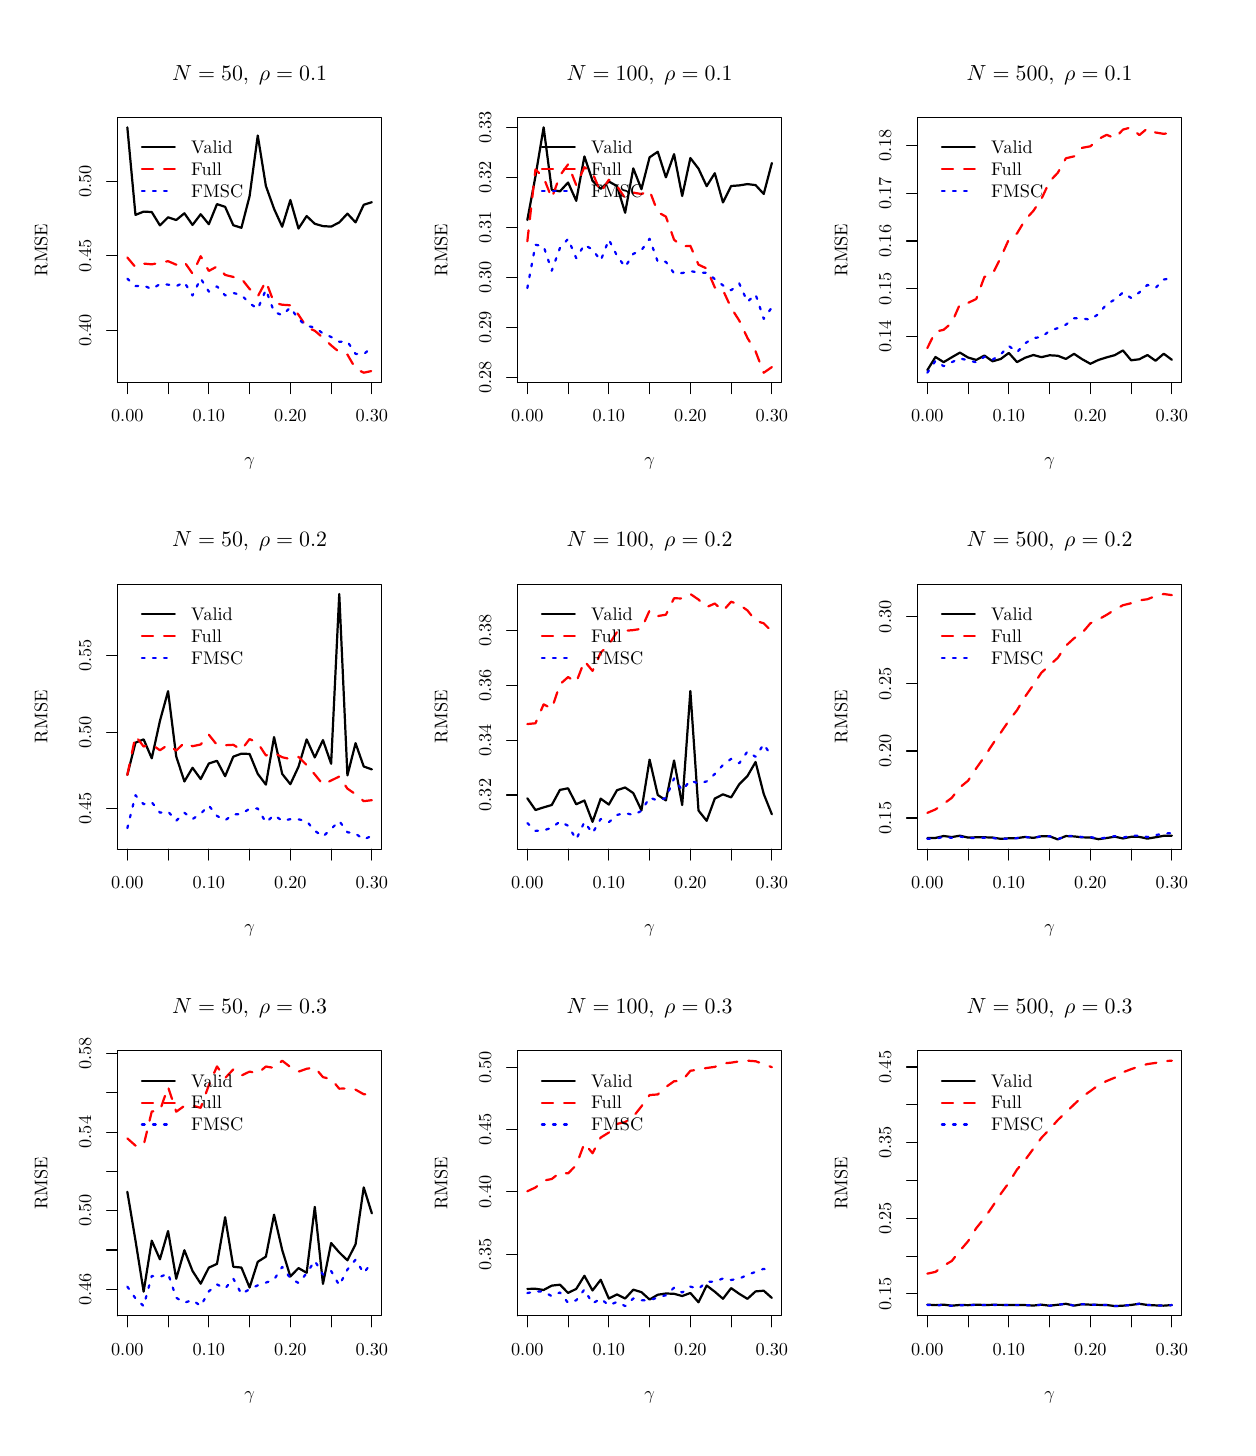
\begin{tikzpicture}[x=1pt,y=1pt]
\definecolor[named]{fillColor}{rgb}{1.00,1.00,1.00}
\path[use as bounding box,fill=fillColor,fill opacity=0.00] (0,0) rectangle (433.62,505.89);
\begin{scope}
\path[clip] ( 32.47,377.65) rectangle (127.91,473.42);
\definecolor[named]{drawColor}{rgb}{0.00,0.00,0.00}

\path[draw=drawColor,line width= 0.8pt,line join=round,line cap=round] ( 36.01,469.87) --
	( 38.95,438.24) --
	( 41.90,439.42) --
	( 44.84,439.26) --
	( 47.79,434.44) --
	( 50.73,437.37) --
	( 53.68,436.38) --
	( 56.63,438.81) --
	( 59.57,434.60) --
	( 62.52,438.47) --
	( 65.46,434.86) --
	( 68.41,442.13) --
	( 71.35,441.13) --
	( 74.30,434.49) --
	( 77.24,433.57) --
	( 80.19,445.01) --
	( 83.14,466.93) --
	( 86.08,448.67) --
	( 89.03,440.43) --
	( 91.97,433.96) --
	( 94.92,443.62) --
	( 97.86,433.31) --
	(100.81,437.81) --
	(103.75,435.02) --
	(106.70,434.18) --
	(109.65,434.00) --
	(112.59,435.51) --
	(115.54,438.69) --
	(118.48,435.52) --
	(121.43,441.89) --
	(124.37,442.82);
\end{scope}
\begin{scope}
\path[clip] (  0.00,  0.00) rectangle (433.62,505.89);
\definecolor[named]{drawColor}{rgb}{0.00,0.00,0.00}

\path[draw=drawColor,line width= 0.4pt,line join=round,line cap=round] ( 36.01,377.65) -- (124.37,377.65);

\path[draw=drawColor,line width= 0.4pt,line join=round,line cap=round] ( 36.01,377.65) -- ( 36.01,373.69);

\path[draw=drawColor,line width= 0.4pt,line join=round,line cap=round] ( 50.73,377.65) -- ( 50.73,373.69);

\path[draw=drawColor,line width= 0.4pt,line join=round,line cap=round] ( 65.46,377.65) -- ( 65.46,373.69);

\path[draw=drawColor,line width= 0.4pt,line join=round,line cap=round] ( 80.19,377.65) -- ( 80.19,373.69);

\path[draw=drawColor,line width= 0.4pt,line join=round,line cap=round] ( 94.92,377.65) -- ( 94.92,373.69);

\path[draw=drawColor,line width= 0.4pt,line join=round,line cap=round] (109.65,377.65) -- (109.65,373.69);

\path[draw=drawColor,line width= 0.4pt,line join=round,line cap=round] (124.37,377.65) -- (124.37,373.69);

\node[text=drawColor,anchor=base,inner sep=0pt, outer sep=0pt, scale=  0.66] at ( 36.01,363.40) {0.00};

\node[text=drawColor,anchor=base,inner sep=0pt, outer sep=0pt, scale=  0.66] at ( 65.46,363.40) {0.10};

\node[text=drawColor,anchor=base,inner sep=0pt, outer sep=0pt, scale=  0.66] at ( 94.92,363.40) {0.20};

\node[text=drawColor,anchor=base,inner sep=0pt, outer sep=0pt, scale=  0.66] at (124.37,363.40) {0.30};

\path[draw=drawColor,line width= 0.4pt,line join=round,line cap=round] ( 32.47,396.54) -- ( 32.47,450.39);

\path[draw=drawColor,line width= 0.4pt,line join=round,line cap=round] ( 32.47,396.54) -- ( 28.51,396.54);

\path[draw=drawColor,line width= 0.4pt,line join=round,line cap=round] ( 32.47,423.46) -- ( 28.51,423.46);

\path[draw=drawColor,line width= 0.4pt,line join=round,line cap=round] ( 32.47,450.39) -- ( 28.51,450.39);

\node[text=drawColor,rotate= 90.00,anchor=base,inner sep=0pt, outer sep=0pt, scale=  0.66] at ( 22.97,396.54) {0.40};

\node[text=drawColor,rotate= 90.00,anchor=base,inner sep=0pt, outer sep=0pt, scale=  0.66] at ( 22.97,423.46) {0.45};

\node[text=drawColor,rotate= 90.00,anchor=base,inner sep=0pt, outer sep=0pt, scale=  0.66] at ( 22.97,450.39) {0.50};

\path[draw=drawColor,line width= 0.4pt,line join=round,line cap=round] ( 32.47,377.65) --
	(127.91,377.65) --
	(127.91,473.42) --
	( 32.47,473.42) --
	( 32.47,377.65);
\end{scope}
\begin{scope}
\path[clip] (  0.00,337.26) rectangle (144.54,505.89);
\definecolor[named]{drawColor}{rgb}{0.00,0.00,0.00}

\node[text=drawColor,anchor=base,inner sep=0pt, outer sep=0pt, scale=  0.79] at ( 80.19,486.92) {\bfseries $N=50, \;\rho=0.1$};

\node[text=drawColor,anchor=base,inner sep=0pt, outer sep=0pt, scale=  0.66] at ( 80.19,347.56) {$\gamma$};

\node[text=drawColor,rotate= 90.00,anchor=base,inner sep=0pt, outer sep=0pt, scale=  0.66] at (  7.13,425.53) {RMSE};
\end{scope}
\begin{scope}
\path[clip] ( 32.47,377.65) rectangle (127.91,473.42);
\definecolor[named]{drawColor}{rgb}{1.00,0.00,0.00}

\path[draw=drawColor,line width= 0.8pt,dash pattern=on 4pt off 4pt ,line join=round,line cap=round] ( 36.01,422.84) --
	( 38.95,419.35) --
	( 41.90,420.63) --
	( 44.84,420.37) --
	( 47.79,420.92) --
	( 50.73,421.51) --
	( 53.68,420.24) --
	( 56.63,421.24) --
	( 59.57,417.02) --
	( 62.52,423.30) --
	( 65.46,417.98) --
	( 68.41,419.59) --
	( 71.35,416.53) --
	( 74.30,415.81) --
	( 77.24,415.20) --
	( 80.19,411.48) --
	( 83.14,408.77) --
	( 86.08,414.25) --
	( 89.03,406.46) --
	( 91.97,405.77) --
	( 94.92,405.57) --
	( 97.86,402.16) --
	(100.81,397.64) --
	(103.75,396.36) --
	(106.70,393.85) --
	(109.65,391.09) --
	(112.59,388.64) --
	(115.54,387.75) --
	(118.48,382.70) --
	(121.43,381.20) --
	(124.37,381.84);
\definecolor[named]{drawColor}{rgb}{0.00,0.00,1.00}

\path[draw=drawColor,line width= 0.8pt,dash pattern=on 1pt off 3pt ,line join=round,line cap=round] ( 36.01,415.20) --
	( 38.95,412.50) --
	( 41.90,412.72) --
	( 44.84,411.42) --
	( 47.79,413.23) --
	( 50.73,413.03) --
	( 53.68,412.47) --
	( 56.63,413.89) --
	( 59.57,409.12) --
	( 62.52,415.25) --
	( 65.46,410.52) --
	( 68.41,412.41) --
	( 71.35,409.14) --
	( 74.30,410.03) --
	( 77.24,409.24) --
	( 80.19,406.31) --
	( 83.14,404.27) --
	( 86.08,411.18) --
	( 89.03,403.23) --
	( 91.97,401.97) --
	( 94.92,404.78) --
	( 97.86,400.56) --
	(100.81,398.08) --
	(103.75,397.59) --
	(106.70,395.38) --
	(109.65,394.13) --
	(112.59,392.41) --
	(115.54,392.46) --
	(118.48,388.01) --
	(121.43,387.91) --
	(124.37,390.35);
\definecolor[named]{drawColor}{rgb}{0.00,0.00,0.00}

\path[draw=drawColor,line width= 0.8pt,line join=round,line cap=round] ( 41.28,462.63) -- ( 53.16,462.63);
\definecolor[named]{drawColor}{rgb}{1.00,0.00,0.00}

\path[draw=drawColor,line width= 0.8pt,dash pattern=on 4pt off 4pt ,line join=round,line cap=round] ( 41.28,454.71) -- ( 53.16,454.71);
\definecolor[named]{drawColor}{rgb}{0.00,0.00,1.00}

\path[draw=drawColor,line width= 0.8pt,dash pattern=on 1pt off 3pt ,line join=round,line cap=round] ( 41.28,446.79) -- ( 53.16,446.79);
\definecolor[named]{drawColor}{rgb}{0.00,0.00,0.00}

\node[text=drawColor,anchor=base west,inner sep=0pt, outer sep=0pt, scale=  0.66] at ( 59.10,460.35) {Valid};

\node[text=drawColor,anchor=base west,inner sep=0pt, outer sep=0pt, scale=  0.66] at ( 59.10,452.43) {Full};

\node[text=drawColor,anchor=base west,inner sep=0pt, outer sep=0pt, scale=  0.66] at ( 59.10,444.51) {FMSC};
\end{scope}
\begin{scope}
\path[clip] (177.01,377.65) rectangle (272.45,473.42);
\definecolor[named]{drawColor}{rgb}{0.00,0.00,0.00}

\path[draw=drawColor,line width= 0.8pt,line join=round,line cap=round] (180.55,436.38) --
	(183.49,452.19) --
	(186.44,469.87) --
	(189.38,447.26) --
	(192.33,446.74) --
	(195.27,449.93) --
	(198.22,443.33) --
	(201.17,459.36) --
	(204.11,450.53) --
	(207.06,447.67) --
	(210.00,450.30) --
	(212.95,448.65) --
	(215.89,439.02) --
	(218.84,455.03) --
	(221.78,447.52) --
	(224.73,459.04) --
	(227.68,461.05) --
	(230.62,451.80) --
	(233.57,460.19) --
	(236.51,445.06) --
	(239.46,458.78) --
	(242.40,454.95) --
	(245.35,448.62) --
	(248.29,453.29) --
	(251.24,442.73) --
	(254.19,448.67) --
	(257.13,448.89) --
	(260.08,449.36) --
	(263.02,449.00) --
	(265.97,445.80) --
	(268.91,456.97);
\end{scope}
\begin{scope}
\path[clip] (  0.00,  0.00) rectangle (433.62,505.89);
\definecolor[named]{drawColor}{rgb}{0.00,0.00,0.00}

\path[draw=drawColor,line width= 0.4pt,line join=round,line cap=round] (180.55,377.65) -- (268.91,377.65);

\path[draw=drawColor,line width= 0.4pt,line join=round,line cap=round] (180.55,377.65) -- (180.55,373.69);

\path[draw=drawColor,line width= 0.4pt,line join=round,line cap=round] (195.27,377.65) -- (195.27,373.69);

\path[draw=drawColor,line width= 0.4pt,line join=round,line cap=round] (210.00,377.65) -- (210.00,373.69);

\path[draw=drawColor,line width= 0.4pt,line join=round,line cap=round] (224.73,377.65) -- (224.73,373.69);

\path[draw=drawColor,line width= 0.4pt,line join=round,line cap=round] (239.46,377.65) -- (239.46,373.69);

\path[draw=drawColor,line width= 0.4pt,line join=round,line cap=round] (254.19,377.65) -- (254.19,373.69);

\path[draw=drawColor,line width= 0.4pt,line join=round,line cap=round] (268.91,377.65) -- (268.91,373.69);

\node[text=drawColor,anchor=base,inner sep=0pt, outer sep=0pt, scale=  0.66] at (180.55,363.40) {0.00};

\node[text=drawColor,anchor=base,inner sep=0pt, outer sep=0pt, scale=  0.66] at (210.00,363.40) {0.10};

\node[text=drawColor,anchor=base,inner sep=0pt, outer sep=0pt, scale=  0.66] at (239.46,363.40) {0.20};

\node[text=drawColor,anchor=base,inner sep=0pt, outer sep=0pt, scale=  0.66] at (268.91,363.40) {0.30};

\path[draw=drawColor,line width= 0.4pt,line join=round,line cap=round] (177.01,379.47) -- (177.01,469.73);

\path[draw=drawColor,line width= 0.4pt,line join=round,line cap=round] (177.01,379.47) -- (173.05,379.47);

\path[draw=drawColor,line width= 0.4pt,line join=round,line cap=round] (177.01,397.52) -- (173.05,397.52);

\path[draw=drawColor,line width= 0.4pt,line join=round,line cap=round] (177.01,415.58) -- (173.05,415.58);

\path[draw=drawColor,line width= 0.4pt,line join=round,line cap=round] (177.01,433.63) -- (173.05,433.63);

\path[draw=drawColor,line width= 0.4pt,line join=round,line cap=round] (177.01,451.68) -- (173.05,451.68);

\path[draw=drawColor,line width= 0.4pt,line join=round,line cap=round] (177.01,469.73) -- (173.05,469.73);

\node[text=drawColor,rotate= 90.00,anchor=base,inner sep=0pt, outer sep=0pt, scale=  0.66] at (167.51,379.47) {0.28};

\node[text=drawColor,rotate= 90.00,anchor=base,inner sep=0pt, outer sep=0pt, scale=  0.66] at (167.51,397.52) {0.29};

\node[text=drawColor,rotate= 90.00,anchor=base,inner sep=0pt, outer sep=0pt, scale=  0.66] at (167.51,415.58) {0.30};

\node[text=drawColor,rotate= 90.00,anchor=base,inner sep=0pt, outer sep=0pt, scale=  0.66] at (167.51,433.63) {0.31};

\node[text=drawColor,rotate= 90.00,anchor=base,inner sep=0pt, outer sep=0pt, scale=  0.66] at (167.51,451.68) {0.32};

\node[text=drawColor,rotate= 90.00,anchor=base,inner sep=0pt, outer sep=0pt, scale=  0.66] at (167.51,469.73) {0.33};

\path[draw=drawColor,line width= 0.4pt,line join=round,line cap=round] (177.01,377.65) --
	(272.45,377.65) --
	(272.45,473.42) --
	(177.01,473.42) --
	(177.01,377.65);
\end{scope}
\begin{scope}
\path[clip] (144.54,337.26) rectangle (289.08,505.89);
\definecolor[named]{drawColor}{rgb}{0.00,0.00,0.00}

\node[text=drawColor,anchor=base,inner sep=0pt, outer sep=0pt, scale=  0.79] at (224.73,486.92) {\bfseries $N=100, \;\rho=0.1$};

\node[text=drawColor,anchor=base,inner sep=0pt, outer sep=0pt, scale=  0.66] at (224.73,347.56) {$\gamma$};

\node[text=drawColor,rotate= 90.00,anchor=base,inner sep=0pt, outer sep=0pt, scale=  0.66] at (151.67,425.53) {RMSE};
\end{scope}
\begin{scope}
\path[clip] (177.01,377.65) rectangle (272.45,473.42);
\definecolor[named]{drawColor}{rgb}{1.00,0.00,0.00}

\path[draw=drawColor,line width= 0.8pt,dash pattern=on 4pt off 4pt ,line join=round,line cap=round] (180.55,428.69) --
	(183.49,454.68) --
	(186.44,451.70) --
	(189.38,444.28) --
	(192.33,452.45) --
	(195.27,456.48) --
	(198.22,449.01) --
	(201.17,455.46) --
	(204.11,453.37) --
	(207.06,446.42) --
	(210.00,450.92) --
	(212.95,448.63) --
	(215.89,444.23) --
	(218.84,446.28) --
	(221.78,445.77) --
	(224.73,446.98) --
	(227.68,439.24) --
	(230.62,437.61) --
	(233.57,429.26) --
	(236.51,426.86) --
	(239.46,427.05) --
	(242.40,420.25) --
	(245.35,418.87) --
	(248.29,412.01) --
	(251.24,411.05) --
	(254.19,404.64) --
	(257.13,400.04) --
	(260.08,393.78) --
	(263.02,388.93) --
	(265.97,381.20) --
	(268.91,383.23);
\definecolor[named]{drawColor}{rgb}{0.00,0.00,1.00}

\path[draw=drawColor,line width= 0.8pt,dash pattern=on 1pt off 3pt ,line join=round,line cap=round] (180.55,411.78) --
	(183.49,427.44) --
	(186.44,426.88) --
	(189.38,418.08) --
	(192.33,426.27) --
	(195.27,429.57) --
	(198.22,422.61) --
	(201.17,427.44) --
	(204.11,425.67) --
	(207.06,421.71) --
	(210.00,429.31) --
	(212.95,423.48) --
	(215.89,419.39) --
	(218.84,424.15) --
	(221.78,425.45) --
	(224.73,429.61) --
	(227.68,421.30) --
	(230.62,421.27) --
	(233.57,417.11) --
	(236.51,417.21) --
	(239.46,417.94) --
	(242.40,417.38) --
	(245.35,417.30) --
	(248.29,415.05) --
	(251.24,412.76) --
	(254.19,410.99) --
	(257.13,413.44) --
	(260.08,406.83) --
	(263.02,409.52) --
	(265.97,400.65) --
	(268.91,404.84);
\definecolor[named]{drawColor}{rgb}{0.00,0.00,0.00}

\path[draw=drawColor,line width= 0.8pt,line join=round,line cap=round] (185.82,462.63) -- (197.70,462.63);
\definecolor[named]{drawColor}{rgb}{1.00,0.00,0.00}

\path[draw=drawColor,line width= 0.8pt,dash pattern=on 4pt off 4pt ,line join=round,line cap=round] (185.82,454.71) -- (197.70,454.71);
\definecolor[named]{drawColor}{rgb}{0.00,0.00,1.00}

\path[draw=drawColor,line width= 0.8pt,dash pattern=on 1pt off 3pt ,line join=round,line cap=round] (185.82,446.79) -- (197.70,446.79);
\definecolor[named]{drawColor}{rgb}{0.00,0.00,0.00}

\node[text=drawColor,anchor=base west,inner sep=0pt, outer sep=0pt, scale=  0.66] at (203.64,460.35) {Valid};

\node[text=drawColor,anchor=base west,inner sep=0pt, outer sep=0pt, scale=  0.66] at (203.64,452.43) {Full};

\node[text=drawColor,anchor=base west,inner sep=0pt, outer sep=0pt, scale=  0.66] at (203.64,444.51) {FMSC};
\end{scope}
\begin{scope}
\path[clip] (321.55,377.65) rectangle (416.99,473.42);
\definecolor[named]{drawColor}{rgb}{0.00,0.00,0.00}

\path[draw=drawColor,line width= 0.8pt,line join=round,line cap=round] (325.09,382.14) --
	(328.03,386.88) --
	(330.98,385.02) --
	(333.92,386.78) --
	(336.87,388.47) --
	(339.81,386.69) --
	(342.76,385.83) --
	(345.71,387.41) --
	(348.65,385.33) --
	(351.60,386.16) --
	(354.54,388.35) --
	(357.49,385.04) --
	(360.43,386.61) --
	(363.38,387.61) --
	(366.32,386.82) --
	(369.27,387.51) --
	(372.22,387.33) --
	(375.16,386.18) --
	(378.11,388.03) --
	(381.05,386.08) --
	(384.00,384.43) --
	(386.94,385.83) --
	(389.89,386.75) --
	(392.83,387.55) --
	(395.78,389.25) --
	(398.73,385.70) --
	(401.67,386.06) --
	(404.62,387.60) --
	(407.56,385.53) --
	(410.51,388.06) --
	(413.45,385.88);
\end{scope}
\begin{scope}
\path[clip] (  0.00,  0.00) rectangle (433.62,505.89);
\definecolor[named]{drawColor}{rgb}{0.00,0.00,0.00}

\path[draw=drawColor,line width= 0.4pt,line join=round,line cap=round] (325.09,377.65) -- (413.45,377.65);

\path[draw=drawColor,line width= 0.4pt,line join=round,line cap=round] (325.09,377.65) -- (325.09,373.69);

\path[draw=drawColor,line width= 0.4pt,line join=round,line cap=round] (339.81,377.65) -- (339.81,373.69);

\path[draw=drawColor,line width= 0.4pt,line join=round,line cap=round] (354.54,377.65) -- (354.54,373.69);

\path[draw=drawColor,line width= 0.4pt,line join=round,line cap=round] (369.27,377.65) -- (369.27,373.69);

\path[draw=drawColor,line width= 0.4pt,line join=round,line cap=round] (384.00,377.65) -- (384.00,373.69);

\path[draw=drawColor,line width= 0.4pt,line join=round,line cap=round] (398.73,377.65) -- (398.73,373.69);

\path[draw=drawColor,line width= 0.4pt,line join=round,line cap=round] (413.45,377.65) -- (413.45,373.69);

\node[text=drawColor,anchor=base,inner sep=0pt, outer sep=0pt, scale=  0.66] at (325.09,363.40) {0.00};

\node[text=drawColor,anchor=base,inner sep=0pt, outer sep=0pt, scale=  0.66] at (354.54,363.40) {0.10};

\node[text=drawColor,anchor=base,inner sep=0pt, outer sep=0pt, scale=  0.66] at (384.00,363.40) {0.20};

\node[text=drawColor,anchor=base,inner sep=0pt, outer sep=0pt, scale=  0.66] at (413.45,363.40) {0.30};

\path[draw=drawColor,line width= 0.4pt,line join=round,line cap=round] (321.55,394.25) -- (321.55,463.36);

\path[draw=drawColor,line width= 0.4pt,line join=round,line cap=round] (321.55,394.25) -- (317.59,394.25);

\path[draw=drawColor,line width= 0.4pt,line join=round,line cap=round] (321.55,411.53) -- (317.59,411.53);

\path[draw=drawColor,line width= 0.4pt,line join=round,line cap=round] (321.55,428.81) -- (317.59,428.81);

\path[draw=drawColor,line width= 0.4pt,line join=round,line cap=round] (321.55,446.09) -- (317.59,446.09);

\path[draw=drawColor,line width= 0.4pt,line join=round,line cap=round] (321.55,463.36) -- (317.59,463.36);

\node[text=drawColor,rotate= 90.00,anchor=base,inner sep=0pt, outer sep=0pt, scale=  0.66] at (312.05,394.25) {0.14};

\node[text=drawColor,rotate= 90.00,anchor=base,inner sep=0pt, outer sep=0pt, scale=  0.66] at (312.05,411.53) {0.15};

\node[text=drawColor,rotate= 90.00,anchor=base,inner sep=0pt, outer sep=0pt, scale=  0.66] at (312.05,428.81) {0.16};

\node[text=drawColor,rotate= 90.00,anchor=base,inner sep=0pt, outer sep=0pt, scale=  0.66] at (312.05,446.09) {0.17};

\node[text=drawColor,rotate= 90.00,anchor=base,inner sep=0pt, outer sep=0pt, scale=  0.66] at (312.05,463.36) {0.18};

\path[draw=drawColor,line width= 0.4pt,line join=round,line cap=round] (321.55,377.65) --
	(416.99,377.65) --
	(416.99,473.42) --
	(321.55,473.42) --
	(321.55,377.65);
\end{scope}
\begin{scope}
\path[clip] (289.08,337.26) rectangle (433.62,505.89);
\definecolor[named]{drawColor}{rgb}{0.00,0.00,0.00}

\node[text=drawColor,anchor=base,inner sep=0pt, outer sep=0pt, scale=  0.79] at (369.27,486.92) {\bfseries $N=500, \;\rho=0.1$};

\node[text=drawColor,anchor=base,inner sep=0pt, outer sep=0pt, scale=  0.66] at (369.27,347.56) {$\gamma$};

\node[text=drawColor,rotate= 90.00,anchor=base,inner sep=0pt, outer sep=0pt, scale=  0.66] at (296.21,425.53) {RMSE};
\end{scope}
\begin{scope}
\path[clip] (321.55,377.65) rectangle (416.99,473.42);
\definecolor[named]{drawColor}{rgb}{1.00,0.00,0.00}

\path[draw=drawColor,line width= 0.8pt,dash pattern=on 4pt off 4pt ,line join=round,line cap=round] (325.09,390.11) --
	(328.03,396.04) --
	(330.98,396.71) --
	(333.92,399.24) --
	(336.87,405.98) --
	(339.81,406.45) --
	(342.76,407.83) --
	(345.71,415.83) --
	(348.65,416.84) --
	(351.60,422.79) --
	(354.54,429.37) --
	(357.49,431.53) --
	(360.43,436.42) --
	(363.38,439.66) --
	(366.32,443.99) --
	(369.27,450.33) --
	(372.22,453.43) --
	(375.16,458.69) --
	(378.11,459.39) --
	(381.05,462.47) --
	(384.00,463.01) --
	(386.94,465.63) --
	(389.89,467.17) --
	(392.83,465.91) --
	(395.78,469.05) --
	(398.73,469.87) --
	(401.67,467.05) --
	(404.62,469.50) --
	(407.56,468.00) --
	(410.51,467.52) --
	(413.45,467.93);
\definecolor[named]{drawColor}{rgb}{0.00,0.00,1.00}

\path[draw=drawColor,line width= 0.8pt,dash pattern=on 1pt off 3pt ,line join=round,line cap=round] (325.09,381.20) --
	(328.03,385.47) --
	(330.98,383.57) --
	(333.92,385.00) --
	(336.87,386.36) --
	(339.81,385.68) --
	(342.76,384.97) --
	(345.71,386.96) --
	(348.65,385.89) --
	(351.60,387.81) --
	(354.54,390.88) --
	(357.49,388.63) --
	(360.43,391.82) --
	(363.38,393.74) --
	(366.32,394.06) --
	(369.27,396.33) --
	(372.22,397.31) --
	(375.16,398.57) --
	(378.11,400.88) --
	(381.05,400.80) --
	(384.00,400.39) --
	(386.94,402.42) --
	(389.89,406.00) --
	(392.83,407.63) --
	(395.78,410.21) --
	(398.73,408.20) --
	(401.67,410.19) --
	(404.62,412.94) --
	(407.56,411.85) --
	(410.51,414.89) --
	(413.45,415.34);
\definecolor[named]{drawColor}{rgb}{0.00,0.00,0.00}

\path[draw=drawColor,line width= 0.8pt,line join=round,line cap=round] (330.36,462.63) -- (342.24,462.63);
\definecolor[named]{drawColor}{rgb}{1.00,0.00,0.00}

\path[draw=drawColor,line width= 0.8pt,dash pattern=on 4pt off 4pt ,line join=round,line cap=round] (330.36,454.71) -- (342.24,454.71);
\definecolor[named]{drawColor}{rgb}{0.00,0.00,1.00}

\path[draw=drawColor,line width= 0.8pt,dash pattern=on 1pt off 3pt ,line join=round,line cap=round] (330.36,446.79) -- (342.24,446.79);
\definecolor[named]{drawColor}{rgb}{0.00,0.00,0.00}

\node[text=drawColor,anchor=base west,inner sep=0pt, outer sep=0pt, scale=  0.66] at (348.18,460.35) {Valid};

\node[text=drawColor,anchor=base west,inner sep=0pt, outer sep=0pt, scale=  0.66] at (348.18,452.43) {Full};

\node[text=drawColor,anchor=base west,inner sep=0pt, outer sep=0pt, scale=  0.66] at (348.18,444.51) {FMSC};
\end{scope}
\begin{scope}
\path[clip] ( 32.47,209.02) rectangle (127.91,304.79);
\definecolor[named]{drawColor}{rgb}{0.00,0.00,0.00}

\path[draw=drawColor,line width= 0.8pt,line join=round,line cap=round] ( 36.01,235.87) --
	( 38.95,247.52) --
	( 41.90,248.72) --
	( 44.84,241.87) --
	( 47.79,255.38) --
	( 50.73,266.12) --
	( 53.68,242.55) --
	( 56.63,233.51) --
	( 59.57,238.45) --
	( 62.52,234.37) --
	( 65.46,240.00) --
	( 68.41,240.96) --
	( 71.35,235.40) --
	( 74.30,242.47) --
	( 77.24,243.56) --
	( 80.19,243.44) --
	( 83.14,236.25) --
	( 86.08,232.37) --
	( 89.03,249.54) --
	( 91.97,236.24) --
	( 94.92,232.52) --
	( 97.86,238.82) --
	(100.81,248.71) --
	(103.75,242.19) --
	(106.70,248.46) --
	(109.65,239.91) --
	(112.59,301.24) --
	(115.54,235.68) --
	(118.48,247.34) --
	(121.43,238.91) --
	(124.37,237.86);
\end{scope}
\begin{scope}
\path[clip] (  0.00,  0.00) rectangle (433.62,505.89);
\definecolor[named]{drawColor}{rgb}{0.00,0.00,0.00}

\path[draw=drawColor,line width= 0.4pt,line join=round,line cap=round] ( 36.01,209.02) -- (124.37,209.02);

\path[draw=drawColor,line width= 0.4pt,line join=round,line cap=round] ( 36.01,209.02) -- ( 36.01,205.06);

\path[draw=drawColor,line width= 0.4pt,line join=round,line cap=round] ( 50.73,209.02) -- ( 50.73,205.06);

\path[draw=drawColor,line width= 0.4pt,line join=round,line cap=round] ( 65.46,209.02) -- ( 65.46,205.06);

\path[draw=drawColor,line width= 0.4pt,line join=round,line cap=round] ( 80.19,209.02) -- ( 80.19,205.06);

\path[draw=drawColor,line width= 0.4pt,line join=round,line cap=round] ( 94.92,209.02) -- ( 94.92,205.06);

\path[draw=drawColor,line width= 0.4pt,line join=round,line cap=round] (109.65,209.02) -- (109.65,205.06);

\path[draw=drawColor,line width= 0.4pt,line join=round,line cap=round] (124.37,209.02) -- (124.37,205.06);

\node[text=drawColor,anchor=base,inner sep=0pt, outer sep=0pt, scale=  0.66] at ( 36.01,194.77) {0.00};

\node[text=drawColor,anchor=base,inner sep=0pt, outer sep=0pt, scale=  0.66] at ( 65.46,194.77) {0.10};

\node[text=drawColor,anchor=base,inner sep=0pt, outer sep=0pt, scale=  0.66] at ( 94.92,194.77) {0.20};

\node[text=drawColor,anchor=base,inner sep=0pt, outer sep=0pt, scale=  0.66] at (124.37,194.77) {0.30};

\path[draw=drawColor,line width= 0.4pt,line join=round,line cap=round] ( 32.47,223.66) -- ( 32.47,278.98);

\path[draw=drawColor,line width= 0.4pt,line join=round,line cap=round] ( 32.47,223.66) -- ( 28.51,223.66);

\path[draw=drawColor,line width= 0.4pt,line join=round,line cap=round] ( 32.47,251.32) -- ( 28.51,251.32);

\path[draw=drawColor,line width= 0.4pt,line join=round,line cap=round] ( 32.47,278.98) -- ( 28.51,278.98);

\node[text=drawColor,rotate= 90.00,anchor=base,inner sep=0pt, outer sep=0pt, scale=  0.66] at ( 22.97,223.66) {0.45};

\node[text=drawColor,rotate= 90.00,anchor=base,inner sep=0pt, outer sep=0pt, scale=  0.66] at ( 22.97,251.32) {0.50};

\node[text=drawColor,rotate= 90.00,anchor=base,inner sep=0pt, outer sep=0pt, scale=  0.66] at ( 22.97,278.98) {0.55};

\path[draw=drawColor,line width= 0.4pt,line join=round,line cap=round] ( 32.47,209.02) --
	(127.91,209.02) --
	(127.91,304.79) --
	( 32.47,304.79) --
	( 32.47,209.02);
\end{scope}
\begin{scope}
\path[clip] (  0.00,168.63) rectangle (144.54,337.26);
\definecolor[named]{drawColor}{rgb}{0.00,0.00,0.00}

\node[text=drawColor,anchor=base,inner sep=0pt, outer sep=0pt, scale=  0.79] at ( 80.19,318.29) {\bfseries $N=50, \;\rho=0.2$};

\node[text=drawColor,anchor=base,inner sep=0pt, outer sep=0pt, scale=  0.66] at ( 80.19,178.93) {$\gamma$};

\node[text=drawColor,rotate= 90.00,anchor=base,inner sep=0pt, outer sep=0pt, scale=  0.66] at (  7.13,256.90) {RMSE};
\end{scope}
\begin{scope}
\path[clip] ( 32.47,209.02) rectangle (127.91,304.79);
\definecolor[named]{drawColor}{rgb}{1.00,0.00,0.00}

\path[draw=drawColor,line width= 0.8pt,dash pattern=on 4pt off 4pt ,line join=round,line cap=round] ( 36.01,235.84) --
	( 38.95,249.97) --
	( 41.90,246.14) --
	( 44.84,246.85) --
	( 47.79,244.79) --
	( 50.73,246.76) --
	( 53.68,244.66) --
	( 56.63,247.53) --
	( 59.57,246.24) --
	( 62.52,246.87) --
	( 65.46,250.40) --
	( 68.41,246.71) --
	( 71.35,246.60) --
	( 74.30,246.75) --
	( 77.24,244.95) --
	( 80.19,248.83) --
	( 83.14,247.41) --
	( 86.08,242.90) --
	( 89.03,243.86) --
	( 91.97,242.26) --
	( 94.92,241.59) --
	( 97.86,242.39) --
	(100.81,239.43) --
	(103.75,236.05) --
	(106.70,232.37) --
	(109.65,233.84) --
	(112.59,235.29) --
	(115.54,230.90) --
	(118.48,228.91) --
	(121.43,226.39) --
	(124.37,226.74);
\definecolor[named]{drawColor}{rgb}{0.00,0.00,1.00}

\path[draw=drawColor,line width= 0.8pt,dash pattern=on 1pt off 3pt ,line join=round,line cap=round] ( 36.01,216.63) --
	( 38.95,228.53) --
	( 41.90,225.29) --
	( 44.84,226.00) --
	( 47.79,222.23) --
	( 50.73,222.63) --
	( 53.68,219.30) --
	( 56.63,222.20) --
	( 59.57,219.91) --
	( 62.52,221.88) --
	( 65.46,224.80) --
	( 68.41,221.05) --
	( 71.35,219.46) --
	( 74.30,221.59) --
	( 77.24,221.75) --
	( 80.19,223.67) --
	( 83.14,223.74) --
	( 86.08,218.69) --
	( 89.03,221.34) --
	( 91.97,219.30) --
	( 94.92,219.87) --
	( 97.86,219.83) --
	(100.81,219.14) --
	(103.75,215.69) --
	(106.70,213.60) --
	(109.65,216.32) --
	(112.59,219.23) --
	(115.54,215.17) --
	(118.48,214.64) --
	(121.43,212.57) --
	(124.37,213.85);
\definecolor[named]{drawColor}{rgb}{0.00,0.00,0.00}

\path[draw=drawColor,line width= 0.8pt,line join=round,line cap=round] ( 41.28,294.00) -- ( 53.16,294.00);
\definecolor[named]{drawColor}{rgb}{1.00,0.00,0.00}

\path[draw=drawColor,line width= 0.8pt,dash pattern=on 4pt off 4pt ,line join=round,line cap=round] ( 41.28,286.08) -- ( 53.16,286.08);
\definecolor[named]{drawColor}{rgb}{0.00,0.00,1.00}

\path[draw=drawColor,line width= 0.8pt,dash pattern=on 1pt off 3pt ,line join=round,line cap=round] ( 41.28,278.16) -- ( 53.16,278.16);
\definecolor[named]{drawColor}{rgb}{0.00,0.00,0.00}

\node[text=drawColor,anchor=base west,inner sep=0pt, outer sep=0pt, scale=  0.66] at ( 59.10,291.72) {Valid};

\node[text=drawColor,anchor=base west,inner sep=0pt, outer sep=0pt, scale=  0.66] at ( 59.10,283.80) {Full};

\node[text=drawColor,anchor=base west,inner sep=0pt, outer sep=0pt, scale=  0.66] at ( 59.10,275.88) {FMSC};
\end{scope}
\begin{scope}
\path[clip] (177.01,209.02) rectangle (272.45,304.79);
\definecolor[named]{drawColor}{rgb}{0.00,0.00,0.00}

\path[draw=drawColor,line width= 0.8pt,line join=round,line cap=round] (180.55,227.43) --
	(183.49,223.19) --
	(186.44,224.14) --
	(189.38,225.00) --
	(192.33,230.46) --
	(195.27,231.04) --
	(198.22,225.26) --
	(201.17,226.62) --
	(204.11,218.91) --
	(207.06,227.29) --
	(210.00,225.16) --
	(212.95,230.35) --
	(215.89,231.33) --
	(218.84,229.29) --
	(221.78,223.08) --
	(224.73,241.40) --
	(227.68,228.64) --
	(230.62,226.65) --
	(233.57,241.09) --
	(236.51,224.98) --
	(239.46,266.19) --
	(242.40,223.00) --
	(245.35,219.29) --
	(248.29,227.32) --
	(251.24,228.85) --
	(254.19,227.75) --
	(257.13,232.51) --
	(260.08,235.45) --
	(263.02,240.55) --
	(265.97,229.00) --
	(268.91,221.64);
\end{scope}
\begin{scope}
\path[clip] (  0.00,  0.00) rectangle (433.62,505.89);
\definecolor[named]{drawColor}{rgb}{0.00,0.00,0.00}

\path[draw=drawColor,line width= 0.4pt,line join=round,line cap=round] (180.55,209.02) -- (268.91,209.02);

\path[draw=drawColor,line width= 0.4pt,line join=round,line cap=round] (180.55,209.02) -- (180.55,205.06);

\path[draw=drawColor,line width= 0.4pt,line join=round,line cap=round] (195.27,209.02) -- (195.27,205.06);

\path[draw=drawColor,line width= 0.4pt,line join=round,line cap=round] (210.00,209.02) -- (210.00,205.06);

\path[draw=drawColor,line width= 0.4pt,line join=round,line cap=round] (224.73,209.02) -- (224.73,205.06);

\path[draw=drawColor,line width= 0.4pt,line join=round,line cap=round] (239.46,209.02) -- (239.46,205.06);

\path[draw=drawColor,line width= 0.4pt,line join=round,line cap=round] (254.19,209.02) -- (254.19,205.06);

\path[draw=drawColor,line width= 0.4pt,line join=round,line cap=round] (268.91,209.02) -- (268.91,205.06);

\node[text=drawColor,anchor=base,inner sep=0pt, outer sep=0pt, scale=  0.66] at (180.55,194.77) {0.00};

\node[text=drawColor,anchor=base,inner sep=0pt, outer sep=0pt, scale=  0.66] at (210.00,194.77) {0.10};

\node[text=drawColor,anchor=base,inner sep=0pt, outer sep=0pt, scale=  0.66] at (239.46,194.77) {0.20};

\node[text=drawColor,anchor=base,inner sep=0pt, outer sep=0pt, scale=  0.66] at (268.91,194.77) {0.30};

\path[draw=drawColor,line width= 0.4pt,line join=round,line cap=round] (177.01,228.62) -- (177.01,287.99);

\path[draw=drawColor,line width= 0.4pt,line join=round,line cap=round] (177.01,228.62) -- (173.05,228.62);

\path[draw=drawColor,line width= 0.4pt,line join=round,line cap=round] (177.01,248.41) -- (173.05,248.41);

\path[draw=drawColor,line width= 0.4pt,line join=round,line cap=round] (177.01,268.20) -- (173.05,268.20);

\path[draw=drawColor,line width= 0.4pt,line join=round,line cap=round] (177.01,287.99) -- (173.05,287.99);

\node[text=drawColor,rotate= 90.00,anchor=base,inner sep=0pt, outer sep=0pt, scale=  0.66] at (167.51,228.62) {0.32};

\node[text=drawColor,rotate= 90.00,anchor=base,inner sep=0pt, outer sep=0pt, scale=  0.66] at (167.51,248.41) {0.34};

\node[text=drawColor,rotate= 90.00,anchor=base,inner sep=0pt, outer sep=0pt, scale=  0.66] at (167.51,268.20) {0.36};

\node[text=drawColor,rotate= 90.00,anchor=base,inner sep=0pt, outer sep=0pt, scale=  0.66] at (167.51,287.99) {0.38};

\path[draw=drawColor,line width= 0.4pt,line join=round,line cap=round] (177.01,209.02) --
	(272.45,209.02) --
	(272.45,304.79) --
	(177.01,304.79) --
	(177.01,209.02);
\end{scope}
\begin{scope}
\path[clip] (144.54,168.63) rectangle (289.08,337.26);
\definecolor[named]{drawColor}{rgb}{0.00,0.00,0.00}

\node[text=drawColor,anchor=base,inner sep=0pt, outer sep=0pt, scale=  0.79] at (224.73,318.29) {\bfseries $N=100, \;\rho=0.2$};

\node[text=drawColor,anchor=base,inner sep=0pt, outer sep=0pt, scale=  0.66] at (224.73,178.93) {$\gamma$};

\node[text=drawColor,rotate= 90.00,anchor=base,inner sep=0pt, outer sep=0pt, scale=  0.66] at (151.67,256.90) {RMSE};
\end{scope}
\begin{scope}
\path[clip] (177.01,209.02) rectangle (272.45,304.79);
\definecolor[named]{drawColor}{rgb}{1.00,0.00,0.00}

\path[draw=drawColor,line width= 0.8pt,dash pattern=on 4pt off 4pt ,line join=round,line cap=round] (180.55,254.25) --
	(183.49,254.53) --
	(186.44,261.38) --
	(189.38,259.81) --
	(192.33,268.60) --
	(195.27,271.23) --
	(198.22,269.36) --
	(201.17,277.04) --
	(204.11,273.45) --
	(207.06,280.04) --
	(210.00,282.92) --
	(212.95,287.51) --
	(215.89,287.95) --
	(218.84,288.20) --
	(221.78,288.67) --
	(224.73,295.29) --
	(227.68,293.27) --
	(230.62,293.76) --
	(233.57,299.70) --
	(236.51,299.63) --
	(239.46,301.24) --
	(242.40,299.24) --
	(245.35,296.51) --
	(248.29,297.81) --
	(251.24,295.13) --
	(254.19,298.45) --
	(257.13,297.42) --
	(260.08,295.31) --
	(263.02,291.61) --
	(265.97,290.65) --
	(268.91,287.68);
\definecolor[named]{drawColor}{rgb}{0.00,0.00,1.00}

\path[draw=drawColor,line width= 0.8pt,dash pattern=on 1pt off 3pt ,line join=round,line cap=round] (180.55,218.48) --
	(183.49,215.65) --
	(186.44,215.81) --
	(189.38,216.78) --
	(192.33,219.03) --
	(195.27,217.51) --
	(198.22,212.57) --
	(201.17,218.86) --
	(204.11,214.81) --
	(207.06,219.96) --
	(210.00,218.77) --
	(212.95,221.40) --
	(215.89,222.11) --
	(218.84,221.37) --
	(221.78,222.87) --
	(224.73,227.69) --
	(227.68,226.58) --
	(230.62,227.52) --
	(233.57,234.60) --
	(236.51,230.33) --
	(239.46,233.88) --
	(242.40,232.73) --
	(245.35,233.54) --
	(248.29,236.21) --
	(251.24,239.45) --
	(254.19,241.66) --
	(257.13,240.09) --
	(260.08,244.31) --
	(263.02,242.42) --
	(265.97,246.99) --
	(268.91,242.49);
\definecolor[named]{drawColor}{rgb}{0.00,0.00,0.00}

\path[draw=drawColor,line width= 0.8pt,line join=round,line cap=round] (185.82,294.00) -- (197.70,294.00);
\definecolor[named]{drawColor}{rgb}{1.00,0.00,0.00}

\path[draw=drawColor,line width= 0.8pt,dash pattern=on 4pt off 4pt ,line join=round,line cap=round] (185.82,286.08) -- (197.70,286.08);
\definecolor[named]{drawColor}{rgb}{0.00,0.00,1.00}

\path[draw=drawColor,line width= 0.8pt,dash pattern=on 1pt off 3pt ,line join=round,line cap=round] (185.82,278.16) -- (197.70,278.16);
\definecolor[named]{drawColor}{rgb}{0.00,0.00,0.00}

\node[text=drawColor,anchor=base west,inner sep=0pt, outer sep=0pt, scale=  0.66] at (203.64,291.72) {Valid};

\node[text=drawColor,anchor=base west,inner sep=0pt, outer sep=0pt, scale=  0.66] at (203.64,283.80) {Full};

\node[text=drawColor,anchor=base west,inner sep=0pt, outer sep=0pt, scale=  0.66] at (203.64,275.88) {FMSC};
\end{scope}
\begin{scope}
\path[clip] (321.55,209.02) rectangle (416.99,304.79);
\definecolor[named]{drawColor}{rgb}{0.00,0.00,0.00}

\path[draw=drawColor,line width= 0.8pt,line join=round,line cap=round] (325.09,213.04) --
	(328.03,213.10) --
	(330.98,213.79) --
	(333.92,213.42) --
	(336.87,213.90) --
	(339.81,213.23) --
	(342.76,213.33) --
	(345.71,213.33) --
	(348.65,213.24) --
	(351.60,212.77) --
	(354.54,212.97) --
	(357.49,213.04) --
	(360.43,213.46) --
	(363.38,213.12) --
	(366.32,213.71) --
	(369.27,213.70) --
	(372.22,212.57) --
	(375.16,213.78) --
	(378.11,213.65) --
	(381.05,213.31) --
	(384.00,213.26) --
	(386.94,212.65) --
	(389.89,213.07) --
	(392.83,213.55) --
	(395.78,212.91) --
	(398.73,213.50) --
	(401.67,213.48) --
	(404.62,212.85) --
	(407.56,213.34) --
	(410.51,213.87) --
	(413.45,213.90);
\end{scope}
\begin{scope}
\path[clip] (  0.00,  0.00) rectangle (433.62,505.89);
\definecolor[named]{drawColor}{rgb}{0.00,0.00,0.00}

\path[draw=drawColor,line width= 0.4pt,line join=round,line cap=round] (325.09,209.02) -- (413.45,209.02);

\path[draw=drawColor,line width= 0.4pt,line join=round,line cap=round] (325.09,209.02) -- (325.09,205.06);

\path[draw=drawColor,line width= 0.4pt,line join=round,line cap=round] (339.81,209.02) -- (339.81,205.06);

\path[draw=drawColor,line width= 0.4pt,line join=round,line cap=round] (354.54,209.02) -- (354.54,205.06);

\path[draw=drawColor,line width= 0.4pt,line join=round,line cap=round] (369.27,209.02) -- (369.27,205.06);

\path[draw=drawColor,line width= 0.4pt,line join=round,line cap=round] (384.00,209.02) -- (384.00,205.06);

\path[draw=drawColor,line width= 0.4pt,line join=round,line cap=round] (398.73,209.02) -- (398.73,205.06);

\path[draw=drawColor,line width= 0.4pt,line join=round,line cap=round] (413.45,209.02) -- (413.45,205.06);

\node[text=drawColor,anchor=base,inner sep=0pt, outer sep=0pt, scale=  0.66] at (325.09,194.77) {0.00};

\node[text=drawColor,anchor=base,inner sep=0pt, outer sep=0pt, scale=  0.66] at (354.54,194.77) {0.10};

\node[text=drawColor,anchor=base,inner sep=0pt, outer sep=0pt, scale=  0.66] at (384.00,194.77) {0.20};

\node[text=drawColor,anchor=base,inner sep=0pt, outer sep=0pt, scale=  0.66] at (413.45,194.77) {0.30};

\path[draw=drawColor,line width= 0.4pt,line join=round,line cap=round] (321.55,220.29) -- (321.55,293.00);

\path[draw=drawColor,line width= 0.4pt,line join=round,line cap=round] (321.55,220.29) -- (317.59,220.29);

\path[draw=drawColor,line width= 0.4pt,line join=round,line cap=round] (321.55,244.53) -- (317.59,244.53);

\path[draw=drawColor,line width= 0.4pt,line join=round,line cap=round] (321.55,268.76) -- (317.59,268.76);

\path[draw=drawColor,line width= 0.4pt,line join=round,line cap=round] (321.55,293.00) -- (317.59,293.00);

\node[text=drawColor,rotate= 90.00,anchor=base,inner sep=0pt, outer sep=0pt, scale=  0.66] at (312.05,220.29) {0.15};

\node[text=drawColor,rotate= 90.00,anchor=base,inner sep=0pt, outer sep=0pt, scale=  0.66] at (312.05,244.53) {0.20};

\node[text=drawColor,rotate= 90.00,anchor=base,inner sep=0pt, outer sep=0pt, scale=  0.66] at (312.05,268.76) {0.25};

\node[text=drawColor,rotate= 90.00,anchor=base,inner sep=0pt, outer sep=0pt, scale=  0.66] at (312.05,293.00) {0.30};

\path[draw=drawColor,line width= 0.4pt,line join=round,line cap=round] (321.55,209.02) --
	(416.99,209.02) --
	(416.99,304.79) --
	(321.55,304.79) --
	(321.55,209.02);
\end{scope}
\begin{scope}
\path[clip] (289.08,168.63) rectangle (433.62,337.26);
\definecolor[named]{drawColor}{rgb}{0.00,0.00,0.00}

\node[text=drawColor,anchor=base,inner sep=0pt, outer sep=0pt, scale=  0.79] at (369.27,318.29) {\bfseries $N=500, \;\rho=0.2$};

\node[text=drawColor,anchor=base,inner sep=0pt, outer sep=0pt, scale=  0.66] at (369.27,178.93) {$\gamma$};

\node[text=drawColor,rotate= 90.00,anchor=base,inner sep=0pt, outer sep=0pt, scale=  0.66] at (296.21,256.90) {RMSE};
\end{scope}
\begin{scope}
\path[clip] (321.55,209.02) rectangle (416.99,304.79);
\definecolor[named]{drawColor}{rgb}{1.00,0.00,0.00}

\path[draw=drawColor,line width= 0.8pt,dash pattern=on 4pt off 4pt ,line join=round,line cap=round] (325.09,222.15) --
	(328.03,223.40) --
	(330.98,225.43) --
	(333.92,227.58) --
	(336.87,231.38) --
	(339.81,233.78) --
	(342.76,238.27) --
	(345.71,242.41) --
	(348.65,246.93) --
	(351.60,251.12) --
	(354.54,255.45) --
	(357.49,259.26) --
	(360.43,264.18) --
	(363.38,268.36) --
	(366.32,272.82) --
	(369.27,275.52) --
	(372.22,278.17) --
	(375.16,282.54) --
	(378.11,285.25) --
	(381.05,287.19) --
	(384.00,290.66) --
	(386.94,292.06) --
	(389.89,293.71) --
	(392.83,295.59) --
	(395.78,297.19) --
	(398.73,297.91) --
	(401.67,298.95) --
	(404.62,299.35) --
	(407.56,300.50) --
	(410.51,301.24) --
	(413.45,300.84);
\definecolor[named]{drawColor}{rgb}{0.00,0.00,1.00}

\path[draw=drawColor,line width= 0.8pt,dash pattern=on 1pt off 3pt ,line join=round,line cap=round] (325.09,212.80) --
	(328.03,212.82) --
	(330.98,213.46) --
	(333.92,213.14) --
	(336.87,213.63) --
	(339.81,213.01) --
	(342.76,213.12) --
	(345.71,213.17) --
	(348.65,213.09) --
	(351.60,212.68) --
	(354.54,212.91) --
	(357.49,213.02) --
	(360.43,213.45) --
	(363.38,213.11) --
	(366.32,213.72) --
	(369.27,213.72) --
	(372.22,212.62) --
	(375.16,213.87) --
	(378.11,213.74) --
	(381.05,213.42) --
	(384.00,213.43) --
	(386.94,212.84) --
	(389.89,213.23) --
	(392.83,213.75) --
	(395.78,213.20) --
	(398.73,213.94) --
	(401.67,213.93) --
	(404.62,213.44) --
	(407.56,214.10) --
	(410.51,214.73) --
	(413.45,214.83);
\definecolor[named]{drawColor}{rgb}{0.00,0.00,0.00}

\path[draw=drawColor,line width= 0.8pt,line join=round,line cap=round] (330.36,294.00) -- (342.24,294.00);
\definecolor[named]{drawColor}{rgb}{1.00,0.00,0.00}

\path[draw=drawColor,line width= 0.8pt,dash pattern=on 4pt off 4pt ,line join=round,line cap=round] (330.36,286.08) -- (342.24,286.08);
\definecolor[named]{drawColor}{rgb}{0.00,0.00,1.00}

\path[draw=drawColor,line width= 0.8pt,dash pattern=on 1pt off 3pt ,line join=round,line cap=round] (330.36,278.16) -- (342.24,278.16);
\definecolor[named]{drawColor}{rgb}{0.00,0.00,0.00}

\node[text=drawColor,anchor=base west,inner sep=0pt, outer sep=0pt, scale=  0.66] at (348.18,291.72) {Valid};

\node[text=drawColor,anchor=base west,inner sep=0pt, outer sep=0pt, scale=  0.66] at (348.18,283.80) {Full};

\node[text=drawColor,anchor=base west,inner sep=0pt, outer sep=0pt, scale=  0.66] at (348.18,275.88) {FMSC};
\end{scope}
\begin{scope}
\path[clip] ( 32.47, 40.39) rectangle (127.91,136.16);
\definecolor[named]{drawColor}{rgb}{0.00,0.00,0.00}

\path[draw=drawColor,line width= 0.8pt,line join=round,line cap=round] ( 36.01, 85.24) --
	( 38.95, 67.69) --
	( 41.90, 49.15) --
	( 44.84, 67.56) --
	( 47.79, 60.84) --
	( 50.73, 71.05) --
	( 53.68, 53.80) --
	( 56.63, 64.12) --
	( 59.57, 56.62) --
	( 62.52, 52.04) --
	( 65.46, 57.83) --
	( 68.41, 59.18) --
	( 71.35, 76.06) --
	( 74.30, 58.14) --
	( 77.24, 57.85) --
	( 80.19, 50.65) --
	( 83.14, 59.93) --
	( 86.08, 61.80) --
	( 89.03, 76.96) --
	( 91.97, 64.20) --
	( 94.92, 54.62) --
	( 97.86, 57.67) --
	(100.81, 55.97) --
	(103.75, 79.79) --
	(106.70, 51.95) --
	(109.65, 66.72) --
	(112.59, 63.32) --
	(115.54, 60.47) --
	(118.48, 66.28) --
	(121.43, 86.83) --
	(124.37, 77.43);
\end{scope}
\begin{scope}
\path[clip] (  0.00,  0.00) rectangle (433.62,505.89);
\definecolor[named]{drawColor}{rgb}{0.00,0.00,0.00}

\path[draw=drawColor,line width= 0.4pt,line join=round,line cap=round] ( 36.01, 40.39) -- (124.37, 40.39);

\path[draw=drawColor,line width= 0.4pt,line join=round,line cap=round] ( 36.01, 40.39) -- ( 36.01, 36.43);

\path[draw=drawColor,line width= 0.4pt,line join=round,line cap=round] ( 50.73, 40.39) -- ( 50.73, 36.43);

\path[draw=drawColor,line width= 0.4pt,line join=round,line cap=round] ( 65.46, 40.39) -- ( 65.46, 36.43);

\path[draw=drawColor,line width= 0.4pt,line join=round,line cap=round] ( 80.19, 40.39) -- ( 80.19, 36.43);

\path[draw=drawColor,line width= 0.4pt,line join=round,line cap=round] ( 94.92, 40.39) -- ( 94.92, 36.43);

\path[draw=drawColor,line width= 0.4pt,line join=round,line cap=round] (109.65, 40.39) -- (109.65, 36.43);

\path[draw=drawColor,line width= 0.4pt,line join=round,line cap=round] (124.37, 40.39) -- (124.37, 36.43);

\node[text=drawColor,anchor=base,inner sep=0pt, outer sep=0pt, scale=  0.66] at ( 36.01, 26.14) {0.00};

\node[text=drawColor,anchor=base,inner sep=0pt, outer sep=0pt, scale=  0.66] at ( 65.46, 26.14) {0.10};

\node[text=drawColor,anchor=base,inner sep=0pt, outer sep=0pt, scale=  0.66] at ( 94.92, 26.14) {0.20};

\node[text=drawColor,anchor=base,inner sep=0pt, outer sep=0pt, scale=  0.66] at (124.37, 26.14) {0.30};

\path[draw=drawColor,line width= 0.4pt,line join=round,line cap=round] ( 32.47, 49.99) -- ( 32.47,135.22);

\path[draw=drawColor,line width= 0.4pt,line join=round,line cap=round] ( 32.47, 49.99) -- ( 28.51, 49.99);

\path[draw=drawColor,line width= 0.4pt,line join=round,line cap=round] ( 32.47, 64.20) -- ( 28.51, 64.20);

\path[draw=drawColor,line width= 0.4pt,line join=round,line cap=round] ( 32.47, 78.40) -- ( 28.51, 78.40);

\path[draw=drawColor,line width= 0.4pt,line join=round,line cap=round] ( 32.47, 92.61) -- ( 28.51, 92.61);

\path[draw=drawColor,line width= 0.4pt,line join=round,line cap=round] ( 32.47,106.81) -- ( 28.51,106.81);

\path[draw=drawColor,line width= 0.4pt,line join=round,line cap=round] ( 32.47,121.02) -- ( 28.51,121.02);

\path[draw=drawColor,line width= 0.4pt,line join=round,line cap=round] ( 32.47,135.22) -- ( 28.51,135.22);

\node[text=drawColor,rotate= 90.00,anchor=base,inner sep=0pt, outer sep=0pt, scale=  0.66] at ( 22.97, 49.99) {0.46};

\node[text=drawColor,rotate= 90.00,anchor=base,inner sep=0pt, outer sep=0pt, scale=  0.66] at ( 22.97, 78.40) {0.50};

\node[text=drawColor,rotate= 90.00,anchor=base,inner sep=0pt, outer sep=0pt, scale=  0.66] at ( 22.97,106.81) {0.54};

\node[text=drawColor,rotate= 90.00,anchor=base,inner sep=0pt, outer sep=0pt, scale=  0.66] at ( 22.97,135.22) {0.58};

\path[draw=drawColor,line width= 0.4pt,line join=round,line cap=round] ( 32.47, 40.39) --
	(127.91, 40.39) --
	(127.91,136.16) --
	( 32.47,136.16) --
	( 32.47, 40.39);
\end{scope}
\begin{scope}
\path[clip] (  0.00,  0.00) rectangle (144.54,168.63);
\definecolor[named]{drawColor}{rgb}{0.00,0.00,0.00}

\node[text=drawColor,anchor=base,inner sep=0pt, outer sep=0pt, scale=  0.79] at ( 80.19,149.66) {\bfseries $N=50, \;\rho=0.3$};

\node[text=drawColor,anchor=base,inner sep=0pt, outer sep=0pt, scale=  0.66] at ( 80.19, 10.30) {$\gamma$};

\node[text=drawColor,rotate= 90.00,anchor=base,inner sep=0pt, outer sep=0pt, scale=  0.66] at (  7.13, 88.27) {RMSE};
\end{scope}
\begin{scope}
\path[clip] ( 32.47, 40.39) rectangle (127.91,136.16);
\definecolor[named]{drawColor}{rgb}{1.00,0.00,0.00}

\path[draw=drawColor,line width= 0.8pt,dash pattern=on 4pt off 4pt ,line join=round,line cap=round] ( 36.01,104.54) --
	( 38.95,101.93) --
	( 41.90,102.06) --
	( 44.84,114.25) --
	( 47.79,114.59) --
	( 50.73,123.12) --
	( 53.68,114.17) --
	( 56.63,116.29) --
	( 59.57,116.38) --
	( 62.52,115.57) --
	( 65.46,123.76) --
	( 68.41,130.54) --
	( 71.35,126.32) --
	( 74.30,129.47) --
	( 77.24,127.25) --
	( 80.19,128.66) --
	( 83.14,128.06) --
	( 86.08,130.50) --
	( 89.03,129.99) --
	( 91.97,132.61) --
	( 94.92,130.30) --
	( 97.86,128.64) --
	(100.81,129.69) --
	(103.75,130.17) --
	(106.70,126.66) --
	(109.65,125.96) --
	(112.59,122.50) --
	(115.54,122.58) --
	(118.48,122.14) --
	(121.43,120.48) --
	(124.37,120.57);
\definecolor[named]{drawColor}{rgb}{0.00,0.00,1.00}

\path[draw=drawColor,line width= 0.8pt,dash pattern=on 1pt off 3pt ,line join=round,line cap=round] ( 36.01, 50.96) --
	( 38.95, 46.72) --
	( 41.90, 43.94) --
	( 44.84, 54.82) --
	( 47.79, 54.46) --
	( 50.73, 55.71) --
	( 53.68, 46.95) --
	( 56.63, 45.17) --
	( 59.57, 46.11) --
	( 62.52, 43.96) --
	( 65.46, 49.25) --
	( 68.41, 51.75) --
	( 71.35, 50.26) --
	( 74.30, 53.86) --
	( 77.24, 48.29) --
	( 80.19, 50.05) --
	( 83.14, 51.43) --
	( 86.08, 52.41) --
	( 89.03, 53.49) --
	( 91.97, 58.09) --
	( 94.92, 53.99) --
	( 97.86, 52.28) --
	(100.81, 55.80) --
	(103.75, 60.29) --
	(106.70, 55.33) --
	(109.65, 56.62) --
	(112.59, 51.44) --
	(115.54, 57.14) --
	(118.48, 60.70) --
	(121.43, 55.86) --
	(124.37, 59.79);
\definecolor[named]{drawColor}{rgb}{0.00,0.00,0.00}

\path[draw=drawColor,line width= 0.8pt,line join=round,line cap=round] ( 41.28,125.37) -- ( 53.16,125.37);
\definecolor[named]{drawColor}{rgb}{1.00,0.00,0.00}

\path[draw=drawColor,line width= 0.8pt,dash pattern=on 4pt off 4pt ,line join=round,line cap=round] ( 41.28,117.45) -- ( 53.16,117.45);
\definecolor[named]{drawColor}{rgb}{0.00,0.00,1.00}

\path[draw=drawColor,line width= 0.8pt,dash pattern=on 1pt off 3pt ,line join=round,line cap=round] ( 41.28,109.53) -- ( 53.16,109.53);
\definecolor[named]{drawColor}{rgb}{0.00,0.00,0.00}

\node[text=drawColor,anchor=base west,inner sep=0pt, outer sep=0pt, scale=  0.66] at ( 59.10,123.09) {Valid};

\node[text=drawColor,anchor=base west,inner sep=0pt, outer sep=0pt, scale=  0.66] at ( 59.10,115.17) {Full};

\node[text=drawColor,anchor=base west,inner sep=0pt, outer sep=0pt, scale=  0.66] at ( 59.10,107.25) {FMSC};
\end{scope}
\begin{scope}
\path[clip] (177.01, 40.39) rectangle (272.45,136.16);
\definecolor[named]{drawColor}{rgb}{0.00,0.00,0.00}

\path[draw=drawColor,line width= 0.8pt,line join=round,line cap=round] (180.55, 50.14) --
	(183.49, 50.19) --
	(186.44, 49.76) --
	(189.38, 51.33) --
	(192.33, 51.65) --
	(195.27, 48.70) --
	(198.22, 50.14) --
	(201.17, 54.88) --
	(204.11, 49.57) --
	(207.06, 53.44) --
	(210.00, 46.66) --
	(212.95, 48.15) --
	(215.89, 46.67) --
	(218.84, 49.87) --
	(221.78, 48.97) --
	(224.73, 46.31) --
	(227.68, 48.04) --
	(230.62, 48.48) --
	(233.57, 48.38) --
	(236.51, 47.57) --
	(239.46, 48.67) --
	(242.40, 45.31) --
	(245.35, 51.37) --
	(248.29, 49.13) --
	(251.24, 46.58) --
	(254.19, 50.42) --
	(257.13, 48.37) --
	(260.08, 46.55) --
	(263.02, 49.24) --
	(265.97, 49.49) --
	(268.91, 46.88);
\end{scope}
\begin{scope}
\path[clip] (  0.00,  0.00) rectangle (433.62,505.89);
\definecolor[named]{drawColor}{rgb}{0.00,0.00,0.00}

\path[draw=drawColor,line width= 0.4pt,line join=round,line cap=round] (180.55, 40.39) -- (268.91, 40.39);

\path[draw=drawColor,line width= 0.4pt,line join=round,line cap=round] (180.55, 40.39) -- (180.55, 36.43);

\path[draw=drawColor,line width= 0.4pt,line join=round,line cap=round] (195.27, 40.39) -- (195.27, 36.43);

\path[draw=drawColor,line width= 0.4pt,line join=round,line cap=round] (210.00, 40.39) -- (210.00, 36.43);

\path[draw=drawColor,line width= 0.4pt,line join=round,line cap=round] (224.73, 40.39) -- (224.73, 36.43);

\path[draw=drawColor,line width= 0.4pt,line join=round,line cap=round] (239.46, 40.39) -- (239.46, 36.43);

\path[draw=drawColor,line width= 0.4pt,line join=round,line cap=round] (254.19, 40.39) -- (254.19, 36.43);

\path[draw=drawColor,line width= 0.4pt,line join=round,line cap=round] (268.91, 40.39) -- (268.91, 36.43);

\node[text=drawColor,anchor=base,inner sep=0pt, outer sep=0pt, scale=  0.66] at (180.55, 26.14) {0.00};

\node[text=drawColor,anchor=base,inner sep=0pt, outer sep=0pt, scale=  0.66] at (210.00, 26.14) {0.10};

\node[text=drawColor,anchor=base,inner sep=0pt, outer sep=0pt, scale=  0.66] at (239.46, 26.14) {0.20};

\node[text=drawColor,anchor=base,inner sep=0pt, outer sep=0pt, scale=  0.66] at (268.91, 26.14) {0.30};

\path[draw=drawColor,line width= 0.4pt,line join=round,line cap=round] (177.01, 62.65) -- (177.01,130.23);

\path[draw=drawColor,line width= 0.4pt,line join=round,line cap=round] (177.01, 62.65) -- (173.05, 62.65);

\path[draw=drawColor,line width= 0.4pt,line join=round,line cap=round] (177.01, 85.18) -- (173.05, 85.18);

\path[draw=drawColor,line width= 0.4pt,line join=round,line cap=round] (177.01,107.70) -- (173.05,107.70);

\path[draw=drawColor,line width= 0.4pt,line join=round,line cap=round] (177.01,130.23) -- (173.05,130.23);

\node[text=drawColor,rotate= 90.00,anchor=base,inner sep=0pt, outer sep=0pt, scale=  0.66] at (167.51, 62.65) {0.35};

\node[text=drawColor,rotate= 90.00,anchor=base,inner sep=0pt, outer sep=0pt, scale=  0.66] at (167.51, 85.18) {0.40};

\node[text=drawColor,rotate= 90.00,anchor=base,inner sep=0pt, outer sep=0pt, scale=  0.66] at (167.51,107.70) {0.45};

\node[text=drawColor,rotate= 90.00,anchor=base,inner sep=0pt, outer sep=0pt, scale=  0.66] at (167.51,130.23) {0.50};

\path[draw=drawColor,line width= 0.4pt,line join=round,line cap=round] (177.01, 40.39) --
	(272.45, 40.39) --
	(272.45,136.16) --
	(177.01,136.16) --
	(177.01, 40.39);
\end{scope}
\begin{scope}
\path[clip] (144.54,  0.00) rectangle (289.08,168.63);
\definecolor[named]{drawColor}{rgb}{0.00,0.00,0.00}

\node[text=drawColor,anchor=base,inner sep=0pt, outer sep=0pt, scale=  0.79] at (224.73,149.66) {\bfseries $N=100, \;\rho=0.3$};

\node[text=drawColor,anchor=base,inner sep=0pt, outer sep=0pt, scale=  0.66] at (224.73, 10.30) {$\gamma$};

\node[text=drawColor,rotate= 90.00,anchor=base,inner sep=0pt, outer sep=0pt, scale=  0.66] at (151.67, 88.27) {RMSE};
\end{scope}
\begin{scope}
\path[clip] (177.01, 40.39) rectangle (272.45,136.16);
\definecolor[named]{drawColor}{rgb}{1.00,0.00,0.00}

\path[draw=drawColor,line width= 0.8pt,dash pattern=on 4pt off 4pt ,line join=round,line cap=round] (180.55, 85.42) --
	(183.49, 86.79) --
	(186.44, 89.28) --
	(189.38, 89.86) --
	(192.33, 92.17) --
	(195.27, 91.89) --
	(198.22, 94.85) --
	(201.17,102.75) --
	(204.11, 99.17) --
	(207.06,104.83) --
	(210.00,106.65) --
	(212.95,109.77) --
	(215.89,110.41) --
	(218.84,112.40) --
	(221.78,116.10) --
	(224.73,120.19) --
	(227.68,120.41) --
	(230.62,123.08) --
	(233.57,125.18) --
	(236.51,125.39) --
	(239.46,128.96) --
	(242.40,129.41) --
	(245.35,129.97) --
	(248.29,130.37) --
	(251.24,131.62) --
	(254.19,131.90) --
	(257.13,132.36) --
	(260.08,132.61) --
	(263.02,132.40) --
	(265.97,131.40) --
	(268.91,130.25);
\definecolor[named]{drawColor}{rgb}{0.00,0.00,1.00}

\path[draw=drawColor,line width= 0.8pt,dash pattern=on 1pt off 3pt ,line join=round,line cap=round] (180.55, 48.63) --
	(183.49, 49.24) --
	(186.44, 49.17) --
	(189.38, 47.51) --
	(192.33, 48.86) --
	(195.27, 45.10) --
	(198.22, 46.03) --
	(201.17, 49.92) --
	(204.11, 44.90) --
	(207.06, 46.60) --
	(210.00, 44.23) --
	(212.95, 45.44) --
	(215.89, 43.94) --
	(218.84, 46.69) --
	(221.78, 46.04) --
	(224.73, 46.00) --
	(227.68, 47.08) --
	(230.62, 47.86) --
	(233.57, 50.58) --
	(236.51, 48.83) --
	(239.46, 50.98) --
	(242.40, 50.17) --
	(245.35, 52.73) --
	(248.29, 52.78) --
	(251.24, 53.92) --
	(254.19, 53.38) --
	(257.13, 53.85) --
	(260.08, 55.22) --
	(263.02, 56.31) --
	(265.97, 57.41) --
	(268.91, 55.79);
\definecolor[named]{drawColor}{rgb}{0.00,0.00,0.00}

\path[draw=drawColor,line width= 0.8pt,line join=round,line cap=round] (185.82,125.37) -- (197.70,125.37);
\definecolor[named]{drawColor}{rgb}{1.00,0.00,0.00}

\path[draw=drawColor,line width= 0.8pt,dash pattern=on 4pt off 4pt ,line join=round,line cap=round] (185.82,117.45) -- (197.70,117.45);
\definecolor[named]{drawColor}{rgb}{0.00,0.00,1.00}

\path[draw=drawColor,line width= 0.8pt,dash pattern=on 1pt off 3pt ,line join=round,line cap=round] (185.82,109.53) -- (197.70,109.53);
\definecolor[named]{drawColor}{rgb}{0.00,0.00,0.00}

\node[text=drawColor,anchor=base west,inner sep=0pt, outer sep=0pt, scale=  0.66] at (203.64,123.09) {Valid};

\node[text=drawColor,anchor=base west,inner sep=0pt, outer sep=0pt, scale=  0.66] at (203.64,115.17) {Full};

\node[text=drawColor,anchor=base west,inner sep=0pt, outer sep=0pt, scale=  0.66] at (203.64,107.25) {FMSC};
\end{scope}
\begin{scope}
\path[clip] (321.55, 40.39) rectangle (416.99,136.16);
\definecolor[named]{drawColor}{rgb}{0.00,0.00,0.00}

\path[draw=drawColor,line width= 0.8pt,line join=round,line cap=round] (325.09, 44.45) --
	(328.03, 44.28) --
	(330.98, 44.45) --
	(333.92, 44.09) --
	(336.87, 44.33) --
	(339.81, 44.27) --
	(342.76, 44.46) --
	(345.71, 44.32) --
	(348.65, 44.39) --
	(351.60, 44.37) --
	(354.54, 44.34) --
	(357.49, 44.29) --
	(360.43, 44.30) --
	(363.38, 44.13) --
	(366.32, 44.44) --
	(369.27, 44.08) --
	(372.22, 44.41) --
	(375.16, 44.76) --
	(378.11, 44.10) --
	(381.05, 44.60) --
	(384.00, 44.44) --
	(386.94, 44.37) --
	(389.89, 44.33) --
	(392.83, 43.94) --
	(395.78, 44.08) --
	(398.73, 44.35) --
	(401.67, 44.77) --
	(404.62, 44.34) --
	(407.56, 44.19) --
	(410.51, 44.09) --
	(413.45, 44.30);
\end{scope}
\begin{scope}
\path[clip] (  0.00,  0.00) rectangle (433.62,505.89);
\definecolor[named]{drawColor}{rgb}{0.00,0.00,0.00}

\path[draw=drawColor,line width= 0.4pt,line join=round,line cap=round] (325.09, 40.39) -- (413.45, 40.39);

\path[draw=drawColor,line width= 0.4pt,line join=round,line cap=round] (325.09, 40.39) -- (325.09, 36.43);

\path[draw=drawColor,line width= 0.4pt,line join=round,line cap=round] (339.81, 40.39) -- (339.81, 36.43);

\path[draw=drawColor,line width= 0.4pt,line join=round,line cap=round] (354.54, 40.39) -- (354.54, 36.43);

\path[draw=drawColor,line width= 0.4pt,line join=round,line cap=round] (369.27, 40.39) -- (369.27, 36.43);

\path[draw=drawColor,line width= 0.4pt,line join=round,line cap=round] (384.00, 40.39) -- (384.00, 36.43);

\path[draw=drawColor,line width= 0.4pt,line join=round,line cap=round] (398.73, 40.39) -- (398.73, 36.43);

\path[draw=drawColor,line width= 0.4pt,line join=round,line cap=round] (413.45, 40.39) -- (413.45, 36.43);

\node[text=drawColor,anchor=base,inner sep=0pt, outer sep=0pt, scale=  0.66] at (325.09, 26.14) {0.00};

\node[text=drawColor,anchor=base,inner sep=0pt, outer sep=0pt, scale=  0.66] at (354.54, 26.14) {0.10};

\node[text=drawColor,anchor=base,inner sep=0pt, outer sep=0pt, scale=  0.66] at (384.00, 26.14) {0.20};

\node[text=drawColor,anchor=base,inner sep=0pt, outer sep=0pt, scale=  0.66] at (413.45, 26.14) {0.30};

\path[draw=drawColor,line width= 0.4pt,line join=round,line cap=round] (321.55, 48.33) -- (321.55,130.32);

\path[draw=drawColor,line width= 0.4pt,line join=round,line cap=round] (321.55, 48.33) -- (317.59, 48.33);

\path[draw=drawColor,line width= 0.4pt,line join=round,line cap=round] (321.55, 61.99) -- (317.59, 61.99);

\path[draw=drawColor,line width= 0.4pt,line join=round,line cap=round] (321.55, 75.66) -- (317.59, 75.66);

\path[draw=drawColor,line width= 0.4pt,line join=round,line cap=round] (321.55, 89.32) -- (317.59, 89.32);

\path[draw=drawColor,line width= 0.4pt,line join=round,line cap=round] (321.55,102.99) -- (317.59,102.99);

\path[draw=drawColor,line width= 0.4pt,line join=round,line cap=round] (321.55,116.65) -- (317.59,116.65);

\path[draw=drawColor,line width= 0.4pt,line join=round,line cap=round] (321.55,130.32) -- (317.59,130.32);

\node[text=drawColor,rotate= 90.00,anchor=base,inner sep=0pt, outer sep=0pt, scale=  0.66] at (312.05, 48.33) {0.15};

\node[text=drawColor,rotate= 90.00,anchor=base,inner sep=0pt, outer sep=0pt, scale=  0.66] at (312.05, 75.66) {0.25};

\node[text=drawColor,rotate= 90.00,anchor=base,inner sep=0pt, outer sep=0pt, scale=  0.66] at (312.05,102.99) {0.35};

\node[text=drawColor,rotate= 90.00,anchor=base,inner sep=0pt, outer sep=0pt, scale=  0.66] at (312.05,130.32) {0.45};

\path[draw=drawColor,line width= 0.4pt,line join=round,line cap=round] (321.55, 40.39) --
	(416.99, 40.39) --
	(416.99,136.16) --
	(321.55,136.16) --
	(321.55, 40.39);
\end{scope}
\begin{scope}
\path[clip] (289.08,  0.00) rectangle (433.62,168.63);
\definecolor[named]{drawColor}{rgb}{0.00,0.00,0.00}

\node[text=drawColor,anchor=base,inner sep=0pt, outer sep=0pt, scale=  0.79] at (369.27,149.66) {\bfseries $N=500, \;\rho=0.3$};

\node[text=drawColor,anchor=base,inner sep=0pt, outer sep=0pt, scale=  0.66] at (369.27, 10.30) {$\gamma$};

\node[text=drawColor,rotate= 90.00,anchor=base,inner sep=0pt, outer sep=0pt, scale=  0.66] at (296.21, 88.27) {RMSE};
\end{scope}
\begin{scope}
\path[clip] (321.55, 40.39) rectangle (416.99,136.16);
\definecolor[named]{drawColor}{rgb}{1.00,0.00,0.00}

\path[draw=drawColor,line width= 0.8pt,dash pattern=on 4pt off 4pt ,line join=round,line cap=round] (325.09, 55.66) --
	(328.03, 56.29) --
	(330.98, 58.51) --
	(333.92, 60.24) --
	(336.87, 63.95) --
	(339.81, 67.37) --
	(342.76, 72.09) --
	(345.71, 75.73) --
	(348.65, 79.95) --
	(351.60, 84.47) --
	(354.54, 88.50) --
	(357.49, 93.27) --
	(360.43, 96.73) --
	(363.38,100.76) --
	(366.32,104.75) --
	(369.27,107.82) --
	(372.22,111.14) --
	(375.16,113.97) --
	(378.11,116.79) --
	(381.05,119.57) --
	(384.00,121.62) --
	(386.94,123.79) --
	(389.89,125.26) --
	(392.83,126.48) --
	(395.78,128.42) --
	(398.73,129.54) --
	(401.67,130.57) --
	(404.62,131.38) --
	(407.56,131.80) --
	(410.51,132.43) --
	(413.45,132.61);
\definecolor[named]{drawColor}{rgb}{0.00,0.00,1.00}

\path[draw=drawColor,line width= 0.8pt,dash pattern=on 1pt off 3pt ,line join=round,line cap=round] (325.09, 44.37) --
	(328.03, 44.17) --
	(330.98, 44.35) --
	(333.92, 44.01) --
	(336.87, 44.24) --
	(339.81, 44.21) --
	(342.76, 44.42) --
	(345.71, 44.29) --
	(348.65, 44.35) --
	(351.60, 44.36) --
	(354.54, 44.34) --
	(357.49, 44.28) --
	(360.43, 44.30) --
	(363.38, 44.12) --
	(366.32, 44.44) --
	(369.27, 44.07) --
	(372.22, 44.41) --
	(375.16, 44.76) --
	(378.11, 44.10) --
	(381.05, 44.60) --
	(384.00, 44.44) --
	(386.94, 44.37) --
	(389.89, 44.33) --
	(392.83, 43.94) --
	(395.78, 44.08) --
	(398.73, 44.35) --
	(401.67, 44.77) --
	(404.62, 44.34) --
	(407.56, 44.19) --
	(410.51, 44.09) --
	(413.45, 44.30);
\definecolor[named]{drawColor}{rgb}{0.00,0.00,0.00}

\path[draw=drawColor,line width= 0.8pt,line join=round,line cap=round] (330.36,125.37) -- (342.24,125.37);
\definecolor[named]{drawColor}{rgb}{1.00,0.00,0.00}

\path[draw=drawColor,line width= 0.8pt,dash pattern=on 4pt off 4pt ,line join=round,line cap=round] (330.36,117.45) -- (342.24,117.45);
\definecolor[named]{drawColor}{rgb}{0.00,0.00,1.00}

\path[draw=drawColor,line width= 0.8pt,dash pattern=on 1pt off 3pt ,line join=round,line cap=round] (330.36,109.53) -- (342.24,109.53);
\definecolor[named]{drawColor}{rgb}{0.00,0.00,0.00}

\node[text=drawColor,anchor=base west,inner sep=0pt, outer sep=0pt, scale=  0.66] at (348.18,123.09) {Valid};

\node[text=drawColor,anchor=base west,inner sep=0pt, outer sep=0pt, scale=  0.66] at (348.18,115.17) {Full};

\node[text=drawColor,anchor=base west,inner sep=0pt, outer sep=0pt, scale=  0.66] at (348.18,107.25) {FMSC};
\end{scope}
\end{tikzpicture}

	\caption{Choose IVs simulation.}
\end{figure}

\begin{figure}
\centering
	% Created by tikzDevice version 0.7.0 on 2014-07-29 12:43:57
% !TEX encoding = UTF-8 Unicode
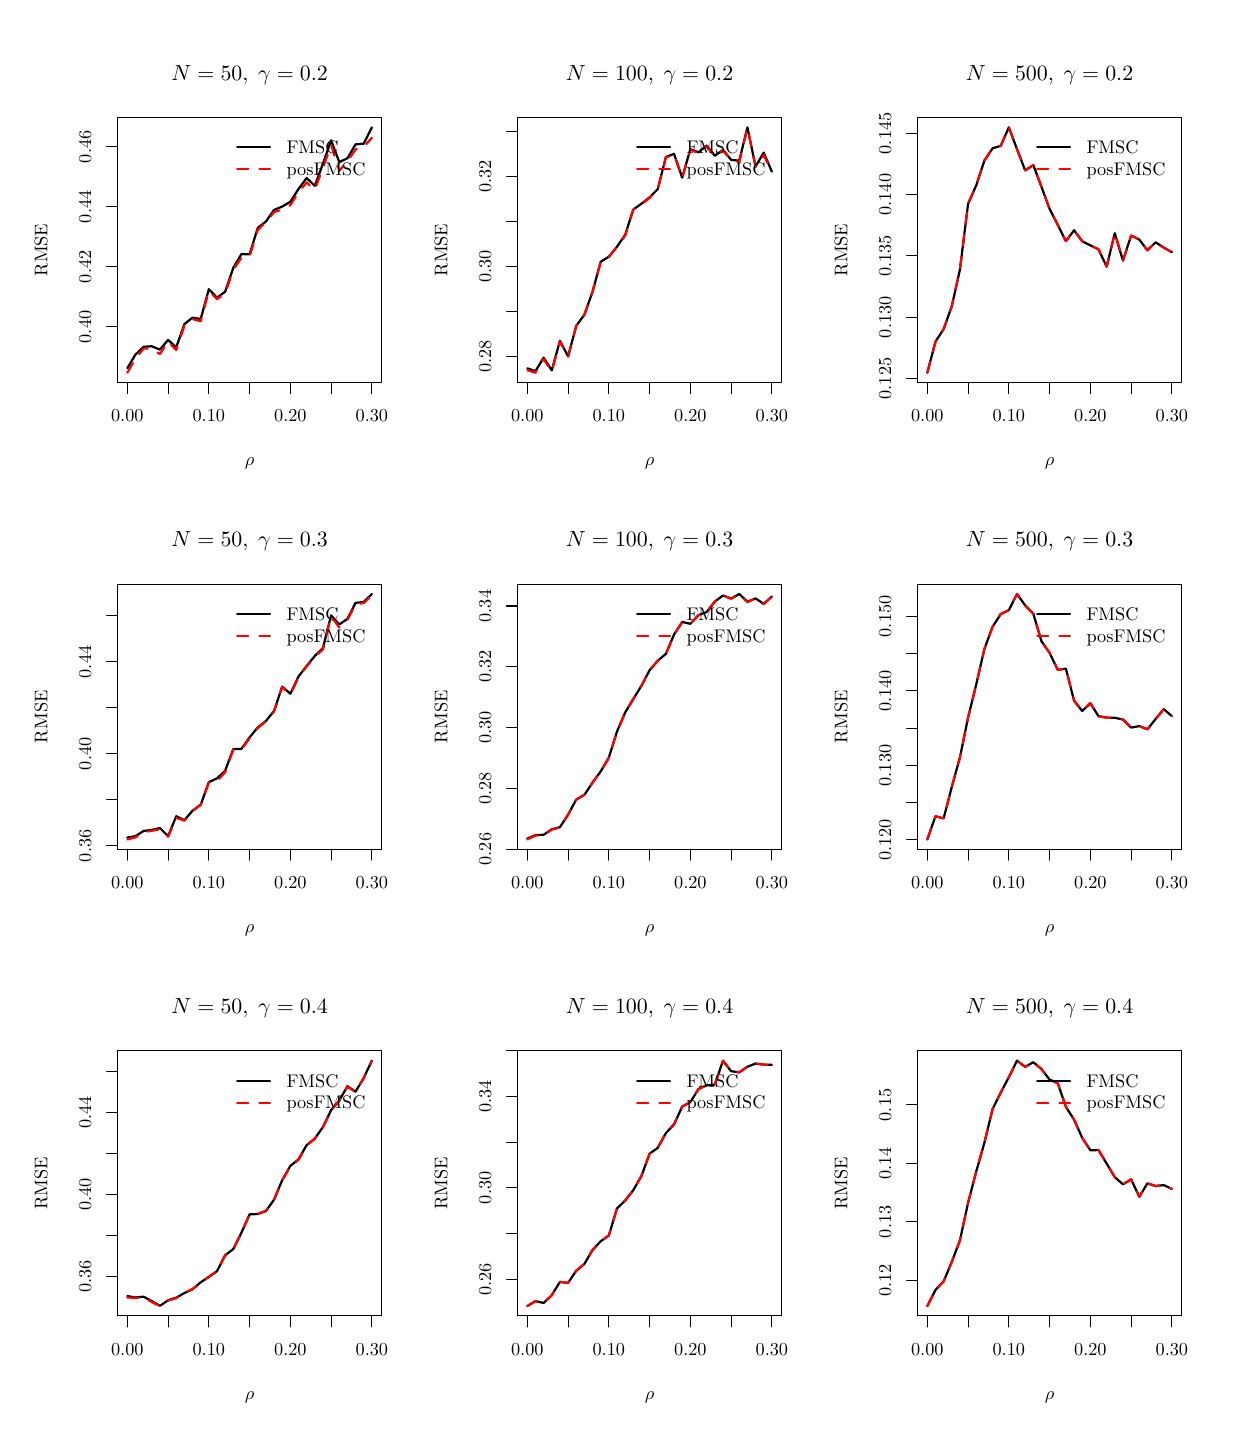
\begin{tikzpicture}[x=1pt,y=1pt]
\definecolor[named]{fillColor}{rgb}{1.00,1.00,1.00}
\path[use as bounding box,fill=fillColor,fill opacity=0.00] (0,0) rectangle (433.62,505.89);
\begin{scope}
\path[clip] ( 32.47,377.65) rectangle (127.91,473.42);
\definecolor[named]{drawColor}{rgb}{0.00,0.00,0.00}

\path[draw=drawColor,line width= 0.8pt,line join=round,line cap=round] ( 36.01,382.83) --
	( 38.95,387.77) --
	( 41.90,390.58) --
	( 44.84,390.76) --
	( 47.79,389.54) --
	( 50.73,393.05) --
	( 53.68,390.37) --
	( 56.63,398.76) --
	( 59.57,401.11) --
	( 62.52,400.61) --
	( 65.46,411.39) --
	( 68.41,408.34) --
	( 71.35,410.47) --
	( 74.30,419.12) --
	( 77.24,424.08) --
	( 80.19,423.97) --
	( 83.14,433.52) --
	( 86.08,435.83) --
	( 89.03,440.02) --
	( 91.97,441.24) --
	( 94.92,442.98) --
	( 97.86,447.59) --
	(100.81,451.55) --
	(103.75,448.74) --
	(106.70,456.75) --
	(109.65,465.17) --
	(112.59,457.33) --
	(115.54,458.69) --
	(118.48,463.72) --
	(121.43,463.97) --
	(124.37,469.87);
\end{scope}
\begin{scope}
\path[clip] (  0.00,  0.00) rectangle (433.62,505.89);
\definecolor[named]{drawColor}{rgb}{0.00,0.00,0.00}

\path[draw=drawColor,line width= 0.4pt,line join=round,line cap=round] ( 36.01,377.65) -- (124.37,377.65);

\path[draw=drawColor,line width= 0.4pt,line join=round,line cap=round] ( 36.01,377.65) -- ( 36.01,373.69);

\path[draw=drawColor,line width= 0.4pt,line join=round,line cap=round] ( 50.73,377.65) -- ( 50.73,373.69);

\path[draw=drawColor,line width= 0.4pt,line join=round,line cap=round] ( 65.46,377.65) -- ( 65.46,373.69);

\path[draw=drawColor,line width= 0.4pt,line join=round,line cap=round] ( 80.19,377.65) -- ( 80.19,373.69);

\path[draw=drawColor,line width= 0.4pt,line join=round,line cap=round] ( 94.92,377.65) -- ( 94.92,373.69);

\path[draw=drawColor,line width= 0.4pt,line join=round,line cap=round] (109.65,377.65) -- (109.65,373.69);

\path[draw=drawColor,line width= 0.4pt,line join=round,line cap=round] (124.37,377.65) -- (124.37,373.69);

\node[text=drawColor,anchor=base,inner sep=0pt, outer sep=0pt, scale=  0.66] at ( 36.01,363.40) {0.00};

\node[text=drawColor,anchor=base,inner sep=0pt, outer sep=0pt, scale=  0.66] at ( 65.46,363.40) {0.10};

\node[text=drawColor,anchor=base,inner sep=0pt, outer sep=0pt, scale=  0.66] at ( 94.92,363.40) {0.20};

\node[text=drawColor,anchor=base,inner sep=0pt, outer sep=0pt, scale=  0.66] at (124.37,363.40) {0.30};

\path[draw=drawColor,line width= 0.4pt,line join=round,line cap=round] ( 32.47,397.76) -- ( 32.47,462.81);

\path[draw=drawColor,line width= 0.4pt,line join=round,line cap=round] ( 32.47,397.76) -- ( 28.51,397.76);

\path[draw=drawColor,line width= 0.4pt,line join=round,line cap=round] ( 32.47,419.45) -- ( 28.51,419.45);

\path[draw=drawColor,line width= 0.4pt,line join=round,line cap=round] ( 32.47,441.13) -- ( 28.51,441.13);

\path[draw=drawColor,line width= 0.4pt,line join=round,line cap=round] ( 32.47,462.81) -- ( 28.51,462.81);

\node[text=drawColor,rotate= 90.00,anchor=base,inner sep=0pt, outer sep=0pt, scale=  0.66] at ( 22.97,397.76) {0.40};

\node[text=drawColor,rotate= 90.00,anchor=base,inner sep=0pt, outer sep=0pt, scale=  0.66] at ( 22.97,419.45) {0.42};

\node[text=drawColor,rotate= 90.00,anchor=base,inner sep=0pt, outer sep=0pt, scale=  0.66] at ( 22.97,441.13) {0.44};

\node[text=drawColor,rotate= 90.00,anchor=base,inner sep=0pt, outer sep=0pt, scale=  0.66] at ( 22.97,462.81) {0.46};

\path[draw=drawColor,line width= 0.4pt,line join=round,line cap=round] ( 32.47,377.65) --
	(127.91,377.65) --
	(127.91,473.42) --
	( 32.47,473.42) --
	( 32.47,377.65);
\end{scope}
\begin{scope}
\path[clip] (  0.00,337.26) rectangle (144.54,505.89);
\definecolor[named]{drawColor}{rgb}{0.00,0.00,0.00}

\node[text=drawColor,anchor=base,inner sep=0pt, outer sep=0pt, scale=  0.79] at ( 80.19,486.92) {\bfseries $N=50, \;\gamma=0.2$};

\node[text=drawColor,anchor=base,inner sep=0pt, outer sep=0pt, scale=  0.66] at ( 80.19,347.56) {$\rho$};

\node[text=drawColor,rotate= 90.00,anchor=base,inner sep=0pt, outer sep=0pt, scale=  0.66] at (  7.13,425.53) {RMSE};
\end{scope}
\begin{scope}
\path[clip] ( 32.47,377.65) rectangle (127.91,473.42);
\definecolor[named]{drawColor}{rgb}{1.00,0.00,0.00}

\path[draw=drawColor,line width= 0.8pt,dash pattern=on 4pt off 4pt ,line join=round,line cap=round] ( 36.01,381.20) --
	( 38.95,386.30) --
	( 41.90,389.99) --
	( 44.84,389.79) --
	( 47.79,387.95) --
	( 50.73,392.49) --
	( 53.68,389.40) --
	( 56.63,398.22) --
	( 59.57,400.59) --
	( 62.52,399.81) --
	( 65.46,410.74) --
	( 68.41,407.80) --
	( 71.35,409.74) --
	( 74.30,418.46) --
	( 77.24,422.74) --
	( 80.19,423.26) --
	( 83.14,432.77) --
	( 86.08,435.64) --
	( 89.03,439.24) --
	( 91.97,440.21) --
	( 94.92,441.75) --
	( 97.86,446.39) --
	(100.81,449.97) --
	(103.75,447.31) --
	(106.70,455.25) --
	(109.65,463.64) --
	(112.59,454.14) --
	(115.54,457.66) --
	(118.48,461.87) --
	(121.43,462.78) --
	(124.37,466.09);
\definecolor[named]{drawColor}{rgb}{0.00,0.00,0.00}

\path[draw=drawColor,line width= 0.8pt,line join=round,line cap=round] ( 75.72,462.63) -- ( 87.60,462.63);
\definecolor[named]{drawColor}{rgb}{1.00,0.00,0.00}

\path[draw=drawColor,line width= 0.8pt,dash pattern=on 4pt off 4pt ,line join=round,line cap=round] ( 75.72,454.71) -- ( 87.60,454.71);
\definecolor[named]{drawColor}{rgb}{0.00,0.00,0.00}

\node[text=drawColor,anchor=base west,inner sep=0pt, outer sep=0pt, scale=  0.66] at ( 93.54,460.35) {FMSC};

\node[text=drawColor,anchor=base west,inner sep=0pt, outer sep=0pt, scale=  0.66] at ( 93.54,452.43) {posFMSC};
\end{scope}
\begin{scope}
\path[clip] (177.01,377.65) rectangle (272.45,473.42);
\definecolor[named]{drawColor}{rgb}{0.00,0.00,0.00}

\path[draw=drawColor,line width= 0.8pt,line join=round,line cap=round] (180.55,382.79) --
	(183.49,381.78) --
	(186.44,386.65) --
	(189.38,382.04) --
	(192.33,392.73) --
	(195.27,387.11) --
	(198.22,398.14) --
	(201.17,402.20) --
	(204.11,410.45) --
	(207.06,421.30) --
	(210.00,423.12) --
	(212.95,426.74) --
	(215.89,430.99) --
	(218.84,440.18) --
	(221.78,442.26) --
	(224.73,444.55) --
	(227.68,447.57) --
	(230.62,459.17) --
	(233.57,460.27) --
	(236.51,451.70) --
	(239.46,461.98) --
	(242.40,460.84) --
	(245.35,463.30) --
	(248.29,459.60) --
	(251.24,461.71) --
	(254.19,458.14) --
	(257.13,457.81) --
	(260.08,469.87) --
	(263.02,455.74) --
	(265.97,460.74) --
	(268.91,453.86);
\end{scope}
\begin{scope}
\path[clip] (  0.00,  0.00) rectangle (433.62,505.89);
\definecolor[named]{drawColor}{rgb}{0.00,0.00,0.00}

\path[draw=drawColor,line width= 0.4pt,line join=round,line cap=round] (180.55,377.65) -- (268.91,377.65);

\path[draw=drawColor,line width= 0.4pt,line join=round,line cap=round] (180.55,377.65) -- (180.55,373.69);

\path[draw=drawColor,line width= 0.4pt,line join=round,line cap=round] (195.27,377.65) -- (195.27,373.69);

\path[draw=drawColor,line width= 0.4pt,line join=round,line cap=round] (210.00,377.65) -- (210.00,373.69);

\path[draw=drawColor,line width= 0.4pt,line join=round,line cap=round] (224.73,377.65) -- (224.73,373.69);

\path[draw=drawColor,line width= 0.4pt,line join=round,line cap=round] (239.46,377.65) -- (239.46,373.69);

\path[draw=drawColor,line width= 0.4pt,line join=round,line cap=round] (254.19,377.65) -- (254.19,373.69);

\path[draw=drawColor,line width= 0.4pt,line join=round,line cap=round] (268.91,377.65) -- (268.91,373.69);

\node[text=drawColor,anchor=base,inner sep=0pt, outer sep=0pt, scale=  0.66] at (180.55,363.40) {0.00};

\node[text=drawColor,anchor=base,inner sep=0pt, outer sep=0pt, scale=  0.66] at (210.00,363.40) {0.10};

\node[text=drawColor,anchor=base,inner sep=0pt, outer sep=0pt, scale=  0.66] at (239.46,363.40) {0.20};

\node[text=drawColor,anchor=base,inner sep=0pt, outer sep=0pt, scale=  0.66] at (268.91,363.40) {0.30};

\path[draw=drawColor,line width= 0.4pt,line join=round,line cap=round] (177.01,387.04) -- (177.01,468.48);

\path[draw=drawColor,line width= 0.4pt,line join=round,line cap=round] (177.01,387.04) -- (173.05,387.04);

\path[draw=drawColor,line width= 0.4pt,line join=round,line cap=round] (177.01,403.33) -- (173.05,403.33);

\path[draw=drawColor,line width= 0.4pt,line join=round,line cap=round] (177.01,419.62) -- (173.05,419.62);

\path[draw=drawColor,line width= 0.4pt,line join=round,line cap=round] (177.01,435.91) -- (173.05,435.91);

\path[draw=drawColor,line width= 0.4pt,line join=round,line cap=round] (177.01,452.19) -- (173.05,452.19);

\path[draw=drawColor,line width= 0.4pt,line join=round,line cap=round] (177.01,468.48) -- (173.05,468.48);

\node[text=drawColor,rotate= 90.00,anchor=base,inner sep=0pt, outer sep=0pt, scale=  0.66] at (167.51,387.04) {0.28};

\node[text=drawColor,rotate= 90.00,anchor=base,inner sep=0pt, outer sep=0pt, scale=  0.66] at (167.51,419.62) {0.30};

\node[text=drawColor,rotate= 90.00,anchor=base,inner sep=0pt, outer sep=0pt, scale=  0.66] at (167.51,452.19) {0.32};

\path[draw=drawColor,line width= 0.4pt,line join=round,line cap=round] (177.01,377.65) --
	(272.45,377.65) --
	(272.45,473.42) --
	(177.01,473.42) --
	(177.01,377.65);
\end{scope}
\begin{scope}
\path[clip] (144.54,337.26) rectangle (289.08,505.89);
\definecolor[named]{drawColor}{rgb}{0.00,0.00,0.00}

\node[text=drawColor,anchor=base,inner sep=0pt, outer sep=0pt, scale=  0.79] at (224.73,486.92) {\bfseries $N=100, \;\gamma=0.2$};

\node[text=drawColor,anchor=base,inner sep=0pt, outer sep=0pt, scale=  0.66] at (224.73,347.56) {$\rho$};

\node[text=drawColor,rotate= 90.00,anchor=base,inner sep=0pt, outer sep=0pt, scale=  0.66] at (151.67,425.53) {RMSE};
\end{scope}
\begin{scope}
\path[clip] (177.01,377.65) rectangle (272.45,473.42);
\definecolor[named]{drawColor}{rgb}{1.00,0.00,0.00}

\path[draw=drawColor,line width= 0.8pt,dash pattern=on 4pt off 4pt ,line join=round,line cap=round] (180.55,382.12) --
	(183.49,381.20) --
	(186.44,386.14) --
	(189.38,381.63) --
	(192.33,392.49) --
	(195.27,386.83) --
	(198.22,398.11) --
	(201.17,402.12) --
	(204.11,410.48) --
	(207.06,421.22) --
	(210.00,423.06) --
	(212.95,426.62) --
	(215.89,430.71) --
	(218.84,440.19) --
	(221.78,441.98) --
	(224.73,444.41) --
	(227.68,447.49) --
	(230.62,458.97) --
	(233.57,460.04) --
	(236.51,451.53) --
	(239.46,461.79) --
	(242.40,460.48) --
	(245.35,462.96) --
	(248.29,459.35) --
	(251.24,461.60) --
	(254.19,457.93) --
	(257.13,457.37) --
	(260.08,469.60) --
	(263.02,455.61) --
	(265.97,459.78) --
	(268.91,453.82);
\definecolor[named]{drawColor}{rgb}{0.00,0.00,0.00}

\path[draw=drawColor,line width= 0.8pt,line join=round,line cap=round] (220.26,462.63) -- (232.14,462.63);
\definecolor[named]{drawColor}{rgb}{1.00,0.00,0.00}

\path[draw=drawColor,line width= 0.8pt,dash pattern=on 4pt off 4pt ,line join=round,line cap=round] (220.26,454.71) -- (232.14,454.71);
\definecolor[named]{drawColor}{rgb}{0.00,0.00,0.00}

\node[text=drawColor,anchor=base west,inner sep=0pt, outer sep=0pt, scale=  0.66] at (238.08,460.35) {FMSC};

\node[text=drawColor,anchor=base west,inner sep=0pt, outer sep=0pt, scale=  0.66] at (238.08,452.43) {posFMSC};
\end{scope}
\begin{scope}
\path[clip] (321.55,377.65) rectangle (416.99,473.42);
\definecolor[named]{drawColor}{rgb}{0.00,0.00,0.00}

\path[draw=drawColor,line width= 0.8pt,line join=round,line cap=round] (325.09,381.20) --
	(328.03,392.44) --
	(330.98,396.99) --
	(333.92,405.21) --
	(336.87,418.47) --
	(339.81,442.22) --
	(342.76,448.92) --
	(345.71,457.86) --
	(348.65,462.29) --
	(351.60,463.17) --
	(354.54,469.87) --
	(357.49,461.99) --
	(360.43,454.31) --
	(363.38,456.21) --
	(366.32,448.42) --
	(369.27,440.38) --
	(372.22,434.62) --
	(375.16,428.75) --
	(378.11,432.68) --
	(381.05,428.71) --
	(384.00,427.22) --
	(386.94,425.79) --
	(389.89,419.54) --
	(392.83,431.63) --
	(395.78,421.70) --
	(398.73,430.77) --
	(401.67,429.32) --
	(404.62,425.43) --
	(407.56,428.32) --
	(410.51,426.42) --
	(413.45,424.76);
\end{scope}
\begin{scope}
\path[clip] (  0.00,  0.00) rectangle (433.62,505.89);
\definecolor[named]{drawColor}{rgb}{0.00,0.00,0.00}

\path[draw=drawColor,line width= 0.4pt,line join=round,line cap=round] (325.09,377.65) -- (413.45,377.65);

\path[draw=drawColor,line width= 0.4pt,line join=round,line cap=round] (325.09,377.65) -- (325.09,373.69);

\path[draw=drawColor,line width= 0.4pt,line join=round,line cap=round] (339.81,377.65) -- (339.81,373.69);

\path[draw=drawColor,line width= 0.4pt,line join=round,line cap=round] (354.54,377.65) -- (354.54,373.69);

\path[draw=drawColor,line width= 0.4pt,line join=round,line cap=round] (369.27,377.65) -- (369.27,373.69);

\path[draw=drawColor,line width= 0.4pt,line join=round,line cap=round] (384.00,377.65) -- (384.00,373.69);

\path[draw=drawColor,line width= 0.4pt,line join=round,line cap=round] (398.73,377.65) -- (398.73,373.69);

\path[draw=drawColor,line width= 0.4pt,line join=round,line cap=round] (413.45,377.65) -- (413.45,373.69);

\node[text=drawColor,anchor=base,inner sep=0pt, outer sep=0pt, scale=  0.66] at (325.09,363.40) {0.00};

\node[text=drawColor,anchor=base,inner sep=0pt, outer sep=0pt, scale=  0.66] at (354.54,363.40) {0.10};

\node[text=drawColor,anchor=base,inner sep=0pt, outer sep=0pt, scale=  0.66] at (384.00,363.40) {0.20};

\node[text=drawColor,anchor=base,inner sep=0pt, outer sep=0pt, scale=  0.66] at (413.45,363.40) {0.30};

\path[draw=drawColor,line width= 0.4pt,line join=round,line cap=round] (321.55,379.11) -- (321.55,467.71);

\path[draw=drawColor,line width= 0.4pt,line join=round,line cap=round] (321.55,379.11) -- (317.59,379.11);

\path[draw=drawColor,line width= 0.4pt,line join=round,line cap=round] (321.55,401.26) -- (317.59,401.26);

\path[draw=drawColor,line width= 0.4pt,line join=round,line cap=round] (321.55,423.41) -- (317.59,423.41);

\path[draw=drawColor,line width= 0.4pt,line join=round,line cap=round] (321.55,445.56) -- (317.59,445.56);

\path[draw=drawColor,line width= 0.4pt,line join=round,line cap=round] (321.55,467.71) -- (317.59,467.71);

\node[text=drawColor,rotate= 90.00,anchor=base,inner sep=0pt, outer sep=0pt, scale=  0.66] at (312.05,379.11) {0.125};

\node[text=drawColor,rotate= 90.00,anchor=base,inner sep=0pt, outer sep=0pt, scale=  0.66] at (312.05,401.26) {0.130};

\node[text=drawColor,rotate= 90.00,anchor=base,inner sep=0pt, outer sep=0pt, scale=  0.66] at (312.05,423.41) {0.135};

\node[text=drawColor,rotate= 90.00,anchor=base,inner sep=0pt, outer sep=0pt, scale=  0.66] at (312.05,445.56) {0.140};

\node[text=drawColor,rotate= 90.00,anchor=base,inner sep=0pt, outer sep=0pt, scale=  0.66] at (312.05,467.71) {0.145};

\path[draw=drawColor,line width= 0.4pt,line join=round,line cap=round] (321.55,377.65) --
	(416.99,377.65) --
	(416.99,473.42) --
	(321.55,473.42) --
	(321.55,377.65);
\end{scope}
\begin{scope}
\path[clip] (289.08,337.26) rectangle (433.62,505.89);
\definecolor[named]{drawColor}{rgb}{0.00,0.00,0.00}

\node[text=drawColor,anchor=base,inner sep=0pt, outer sep=0pt, scale=  0.79] at (369.27,486.92) {\bfseries $N=500, \;\gamma=0.2$};

\node[text=drawColor,anchor=base,inner sep=0pt, outer sep=0pt, scale=  0.66] at (369.27,347.56) {$\rho$};

\node[text=drawColor,rotate= 90.00,anchor=base,inner sep=0pt, outer sep=0pt, scale=  0.66] at (296.21,425.54) {RMSE};
\end{scope}
\begin{scope}
\path[clip] (321.55,377.65) rectangle (416.99,473.42);
\definecolor[named]{drawColor}{rgb}{1.00,0.00,0.00}

\path[draw=drawColor,line width= 0.8pt,dash pattern=on 4pt off 4pt ,line join=round,line cap=round] (325.09,381.22) --
	(328.03,392.43) --
	(330.98,396.99) --
	(333.92,405.18) --
	(336.87,418.52) --
	(339.81,442.20) --
	(342.76,448.93) --
	(345.71,457.87) --
	(348.65,462.28) --
	(351.60,463.17) --
	(354.54,469.86) --
	(357.49,462.00) --
	(360.43,454.31) --
	(363.38,456.21) --
	(366.32,448.42) --
	(369.27,440.38) --
	(372.22,434.62) --
	(375.16,428.75) --
	(378.11,432.68) --
	(381.05,428.71) --
	(384.00,427.22) --
	(386.94,425.79) --
	(389.89,419.54) --
	(392.83,431.63) --
	(395.78,421.70) --
	(398.73,430.77) --
	(401.67,429.32) --
	(404.62,425.43) --
	(407.56,428.32) --
	(410.51,426.42) --
	(413.45,424.76);
\definecolor[named]{drawColor}{rgb}{0.00,0.00,0.00}

\path[draw=drawColor,line width= 0.8pt,line join=round,line cap=round] (364.80,462.63) -- (376.68,462.63);
\definecolor[named]{drawColor}{rgb}{1.00,0.00,0.00}

\path[draw=drawColor,line width= 0.8pt,dash pattern=on 4pt off 4pt ,line join=round,line cap=round] (364.80,454.71) -- (376.68,454.71);
\definecolor[named]{drawColor}{rgb}{0.00,0.00,0.00}

\node[text=drawColor,anchor=base west,inner sep=0pt, outer sep=0pt, scale=  0.66] at (382.62,460.35) {FMSC};

\node[text=drawColor,anchor=base west,inner sep=0pt, outer sep=0pt, scale=  0.66] at (382.62,452.43) {posFMSC};
\end{scope}
\begin{scope}
\path[clip] ( 32.47,209.02) rectangle (127.91,304.79);
\definecolor[named]{drawColor}{rgb}{0.00,0.00,0.00}

\path[draw=drawColor,line width= 0.8pt,line join=round,line cap=round] ( 36.01,213.24) --
	( 38.95,213.74) --
	( 41.90,215.64) --
	( 44.84,215.99) --
	( 47.79,216.68) --
	( 50.73,213.75) --
	( 53.68,220.94) --
	( 56.63,219.49) --
	( 59.57,222.95) --
	( 62.52,225.08) --
	( 65.46,233.27) --
	( 68.41,234.62) --
	( 71.35,237.36) --
	( 74.30,245.24) --
	( 77.24,245.27) --
	( 80.19,249.45) --
	( 83.14,253.02) --
	( 86.08,255.34) --
	( 89.03,259.02) --
	( 91.97,267.76) --
	( 94.92,265.22) --
	( 97.86,271.41) --
	(100.81,275.25) --
	(103.75,278.84) --
	(106.70,281.76) --
	(109.65,293.53) --
	(112.59,290.22) --
	(115.54,292.28) --
	(118.48,298.05) --
	(121.43,298.36) --
	(124.37,301.24);
\end{scope}
\begin{scope}
\path[clip] (  0.00,  0.00) rectangle (433.62,505.89);
\definecolor[named]{drawColor}{rgb}{0.00,0.00,0.00}

\path[draw=drawColor,line width= 0.4pt,line join=round,line cap=round] ( 36.01,209.02) -- (124.37,209.02);

\path[draw=drawColor,line width= 0.4pt,line join=round,line cap=round] ( 36.01,209.02) -- ( 36.01,205.06);

\path[draw=drawColor,line width= 0.4pt,line join=round,line cap=round] ( 50.73,209.02) -- ( 50.73,205.06);

\path[draw=drawColor,line width= 0.4pt,line join=round,line cap=round] ( 65.46,209.02) -- ( 65.46,205.06);

\path[draw=drawColor,line width= 0.4pt,line join=round,line cap=round] ( 80.19,209.02) -- ( 80.19,205.06);

\path[draw=drawColor,line width= 0.4pt,line join=round,line cap=round] ( 94.92,209.02) -- ( 94.92,205.06);

\path[draw=drawColor,line width= 0.4pt,line join=round,line cap=round] (109.65,209.02) -- (109.65,205.06);

\path[draw=drawColor,line width= 0.4pt,line join=round,line cap=round] (124.37,209.02) -- (124.37,205.06);

\node[text=drawColor,anchor=base,inner sep=0pt, outer sep=0pt, scale=  0.66] at ( 36.01,194.77) {0.00};

\node[text=drawColor,anchor=base,inner sep=0pt, outer sep=0pt, scale=  0.66] at ( 65.46,194.77) {0.10};

\node[text=drawColor,anchor=base,inner sep=0pt, outer sep=0pt, scale=  0.66] at ( 94.92,194.77) {0.20};

\node[text=drawColor,anchor=base,inner sep=0pt, outer sep=0pt, scale=  0.66] at (124.37,194.77) {0.30};

\path[draw=drawColor,line width= 0.4pt,line join=round,line cap=round] ( 32.47,210.27) -- ( 32.47,293.32);

\path[draw=drawColor,line width= 0.4pt,line join=round,line cap=round] ( 32.47,210.27) -- ( 28.51,210.27);

\path[draw=drawColor,line width= 0.4pt,line join=round,line cap=round] ( 32.47,226.88) -- ( 28.51,226.88);

\path[draw=drawColor,line width= 0.4pt,line join=round,line cap=round] ( 32.47,243.49) -- ( 28.51,243.49);

\path[draw=drawColor,line width= 0.4pt,line join=round,line cap=round] ( 32.47,260.10) -- ( 28.51,260.10);

\path[draw=drawColor,line width= 0.4pt,line join=round,line cap=round] ( 32.47,276.71) -- ( 28.51,276.71);

\path[draw=drawColor,line width= 0.4pt,line join=round,line cap=round] ( 32.47,293.32) -- ( 28.51,293.32);

\node[text=drawColor,rotate= 90.00,anchor=base,inner sep=0pt, outer sep=0pt, scale=  0.66] at ( 22.97,210.27) {0.36};

\node[text=drawColor,rotate= 90.00,anchor=base,inner sep=0pt, outer sep=0pt, scale=  0.66] at ( 22.97,243.49) {0.40};

\node[text=drawColor,rotate= 90.00,anchor=base,inner sep=0pt, outer sep=0pt, scale=  0.66] at ( 22.97,276.71) {0.44};

\path[draw=drawColor,line width= 0.4pt,line join=round,line cap=round] ( 32.47,209.02) --
	(127.91,209.02) --
	(127.91,304.79) --
	( 32.47,304.79) --
	( 32.47,209.02);
\end{scope}
\begin{scope}
\path[clip] (  0.00,168.63) rectangle (144.54,337.26);
\definecolor[named]{drawColor}{rgb}{0.00,0.00,0.00}

\node[text=drawColor,anchor=base,inner sep=0pt, outer sep=0pt, scale=  0.79] at ( 80.19,318.29) {\bfseries $N=50, \;\gamma=0.3$};

\node[text=drawColor,anchor=base,inner sep=0pt, outer sep=0pt, scale=  0.66] at ( 80.19,178.93) {$\rho$};

\node[text=drawColor,rotate= 90.00,anchor=base,inner sep=0pt, outer sep=0pt, scale=  0.66] at (  7.13,256.90) {RMSE};
\end{scope}
\begin{scope}
\path[clip] ( 32.47,209.02) rectangle (127.91,304.79);
\definecolor[named]{drawColor}{rgb}{1.00,0.00,0.00}

\path[draw=drawColor,line width= 0.8pt,dash pattern=on 4pt off 4pt ,line join=round,line cap=round] ( 36.01,212.57) --
	( 38.95,213.30) --
	( 41.90,215.21) --
	( 44.84,215.68) --
	( 47.79,216.24) --
	( 50.73,213.54) --
	( 53.68,220.36) --
	( 56.63,219.34) --
	( 59.57,222.76) --
	( 62.52,225.09) --
	( 65.46,233.15) --
	( 68.41,233.65) --
	( 71.35,236.87) --
	( 74.30,245.05) --
	( 77.24,245.07) --
	( 80.19,249.11) --
	( 83.14,252.77) --
	( 86.08,255.25) --
	( 89.03,258.84) --
	( 91.97,267.59) --
	( 94.92,265.00) --
	( 97.86,271.05) --
	(100.81,275.11) --
	(103.75,278.55) --
	(106.70,281.22) --
	(109.65,293.22) --
	(112.59,289.17) --
	(115.54,291.85) --
	(118.48,297.60) --
	(121.43,297.97) --
	(124.37,300.79);
\definecolor[named]{drawColor}{rgb}{0.00,0.00,0.00}

\path[draw=drawColor,line width= 0.8pt,line join=round,line cap=round] ( 75.72,294.00) -- ( 87.60,294.00);
\definecolor[named]{drawColor}{rgb}{1.00,0.00,0.00}

\path[draw=drawColor,line width= 0.8pt,dash pattern=on 4pt off 4pt ,line join=round,line cap=round] ( 75.72,286.08) -- ( 87.60,286.08);
\definecolor[named]{drawColor}{rgb}{0.00,0.00,0.00}

\node[text=drawColor,anchor=base west,inner sep=0pt, outer sep=0pt, scale=  0.66] at ( 93.54,291.72) {FMSC};

\node[text=drawColor,anchor=base west,inner sep=0pt, outer sep=0pt, scale=  0.66] at ( 93.54,283.80) {posFMSC};
\end{scope}
\begin{scope}
\path[clip] (177.01,209.02) rectangle (272.45,304.79);
\definecolor[named]{drawColor}{rgb}{0.00,0.00,0.00}

\path[draw=drawColor,line width= 0.8pt,line join=round,line cap=round] (180.55,212.87) --
	(183.49,214.11) --
	(186.44,214.24) --
	(189.38,216.23) --
	(192.33,216.99) --
	(195.27,221.48) --
	(198.22,226.97) --
	(201.17,228.69) --
	(204.11,233.07) --
	(207.06,237.16) --
	(210.00,242.13) --
	(212.95,251.56) --
	(215.89,258.40) --
	(218.84,263.32) --
	(221.78,268.05) --
	(224.73,273.69) --
	(227.68,277.12) --
	(230.62,279.63) --
	(233.57,286.60) --
	(236.51,291.13) --
	(239.46,290.47) --
	(242.40,293.63) --
	(245.35,294.74) --
	(248.29,298.52) --
	(251.24,300.69) --
	(254.19,299.59) --
	(257.13,301.24) --
	(260.08,298.43) --
	(263.02,299.64) --
	(265.97,297.70) --
	(268.91,300.34);
\end{scope}
\begin{scope}
\path[clip] (  0.00,  0.00) rectangle (433.62,505.89);
\definecolor[named]{drawColor}{rgb}{0.00,0.00,0.00}

\path[draw=drawColor,line width= 0.4pt,line join=round,line cap=round] (180.55,209.02) -- (268.91,209.02);

\path[draw=drawColor,line width= 0.4pt,line join=round,line cap=round] (180.55,209.02) -- (180.55,205.06);

\path[draw=drawColor,line width= 0.4pt,line join=round,line cap=round] (195.27,209.02) -- (195.27,205.06);

\path[draw=drawColor,line width= 0.4pt,line join=round,line cap=round] (210.00,209.02) -- (210.00,205.06);

\path[draw=drawColor,line width= 0.4pt,line join=round,line cap=round] (224.73,209.02) -- (224.73,205.06);

\path[draw=drawColor,line width= 0.4pt,line join=round,line cap=round] (239.46,209.02) -- (239.46,205.06);

\path[draw=drawColor,line width= 0.4pt,line join=round,line cap=round] (254.19,209.02) -- (254.19,205.06);

\path[draw=drawColor,line width= 0.4pt,line join=round,line cap=round] (268.91,209.02) -- (268.91,205.06);

\node[text=drawColor,anchor=base,inner sep=0pt, outer sep=0pt, scale=  0.66] at (180.55,194.77) {0.00};

\node[text=drawColor,anchor=base,inner sep=0pt, outer sep=0pt, scale=  0.66] at (210.00,194.77) {0.10};

\node[text=drawColor,anchor=base,inner sep=0pt, outer sep=0pt, scale=  0.66] at (239.46,194.77) {0.20};

\node[text=drawColor,anchor=base,inner sep=0pt, outer sep=0pt, scale=  0.66] at (268.91,194.77) {0.30};

\path[draw=drawColor,line width= 0.4pt,line join=round,line cap=round] (177.01,209.07) -- (177.01,296.92);

\path[draw=drawColor,line width= 0.4pt,line join=round,line cap=round] (177.01,209.07) -- (173.05,209.07);

\path[draw=drawColor,line width= 0.4pt,line join=round,line cap=round] (177.01,231.04) -- (173.05,231.04);

\path[draw=drawColor,line width= 0.4pt,line join=round,line cap=round] (177.01,253.00) -- (173.05,253.00);

\path[draw=drawColor,line width= 0.4pt,line join=round,line cap=round] (177.01,274.96) -- (173.05,274.96);

\path[draw=drawColor,line width= 0.4pt,line join=round,line cap=round] (177.01,296.92) -- (173.05,296.92);

\node[text=drawColor,rotate= 90.00,anchor=base,inner sep=0pt, outer sep=0pt, scale=  0.66] at (167.51,209.07) {0.26};

\node[text=drawColor,rotate= 90.00,anchor=base,inner sep=0pt, outer sep=0pt, scale=  0.66] at (167.51,231.04) {0.28};

\node[text=drawColor,rotate= 90.00,anchor=base,inner sep=0pt, outer sep=0pt, scale=  0.66] at (167.51,253.00) {0.30};

\node[text=drawColor,rotate= 90.00,anchor=base,inner sep=0pt, outer sep=0pt, scale=  0.66] at (167.51,274.96) {0.32};

\node[text=drawColor,rotate= 90.00,anchor=base,inner sep=0pt, outer sep=0pt, scale=  0.66] at (167.51,296.92) {0.34};

\path[draw=drawColor,line width= 0.4pt,line join=round,line cap=round] (177.01,209.02) --
	(272.45,209.02) --
	(272.45,304.79) --
	(177.01,304.79) --
	(177.01,209.02);
\end{scope}
\begin{scope}
\path[clip] (144.54,168.63) rectangle (289.08,337.26);
\definecolor[named]{drawColor}{rgb}{0.00,0.00,0.00}

\node[text=drawColor,anchor=base,inner sep=0pt, outer sep=0pt, scale=  0.79] at (224.73,318.29) {\bfseries $N=100, \;\gamma=0.3$};

\node[text=drawColor,anchor=base,inner sep=0pt, outer sep=0pt, scale=  0.66] at (224.73,178.93) {$\rho$};

\node[text=drawColor,rotate= 90.00,anchor=base,inner sep=0pt, outer sep=0pt, scale=  0.66] at (151.67,256.90) {RMSE};
\end{scope}
\begin{scope}
\path[clip] (177.01,209.02) rectangle (272.45,304.79);
\definecolor[named]{drawColor}{rgb}{1.00,0.00,0.00}

\path[draw=drawColor,line width= 0.8pt,dash pattern=on 4pt off 4pt ,line join=round,line cap=round] (180.55,212.57) --
	(183.49,213.96) --
	(186.44,214.05) --
	(189.38,216.09) --
	(192.33,216.91) --
	(195.27,221.49) --
	(198.22,226.91) --
	(201.17,228.72) --
	(204.11,233.03) --
	(207.06,237.17) --
	(210.00,242.01) --
	(212.95,251.55) --
	(215.89,258.33) --
	(218.84,263.35) --
	(221.78,268.08) --
	(224.73,273.70) --
	(227.68,277.09) --
	(230.62,279.63) --
	(233.57,286.54) --
	(236.51,291.06) --
	(239.46,290.46) --
	(242.40,293.54) --
	(245.35,294.70) --
	(248.29,298.46) --
	(251.24,300.66) --
	(254.19,299.55) --
	(257.13,301.17) --
	(260.08,298.34) --
	(263.02,299.59) --
	(265.97,297.61) --
	(268.91,300.32);
\definecolor[named]{drawColor}{rgb}{0.00,0.00,0.00}

\path[draw=drawColor,line width= 0.8pt,line join=round,line cap=round] (220.26,294.00) -- (232.14,294.00);
\definecolor[named]{drawColor}{rgb}{1.00,0.00,0.00}

\path[draw=drawColor,line width= 0.8pt,dash pattern=on 4pt off 4pt ,line join=round,line cap=round] (220.26,286.08) -- (232.14,286.08);
\definecolor[named]{drawColor}{rgb}{0.00,0.00,0.00}

\node[text=drawColor,anchor=base west,inner sep=0pt, outer sep=0pt, scale=  0.66] at (238.08,291.72) {FMSC};

\node[text=drawColor,anchor=base west,inner sep=0pt, outer sep=0pt, scale=  0.66] at (238.08,283.80) {posFMSC};
\end{scope}
\begin{scope}
\path[clip] (321.55,209.02) rectangle (416.99,304.79);
\definecolor[named]{drawColor}{rgb}{0.00,0.00,0.00}

\path[draw=drawColor,line width= 0.8pt,line join=round,line cap=round] (325.09,212.57) --
	(328.03,220.93) --
	(330.98,220.17) --
	(333.92,231.51) --
	(336.87,242.21) --
	(339.81,256.57) --
	(342.76,268.58) --
	(345.71,281.38) --
	(348.65,289.36) --
	(351.60,294.00) --
	(354.54,295.40) --
	(357.49,301.24) --
	(360.43,297.15) --
	(363.38,294.11) --
	(366.32,284.18) --
	(369.27,279.94) --
	(372.22,273.82) --
	(375.16,274.28) --
	(378.11,262.70) --
	(381.05,258.96) --
	(384.00,261.78) --
	(386.94,257.08) --
	(389.89,256.58) --
	(392.83,256.50) --
	(395.78,255.90) --
	(398.73,252.98) --
	(401.67,253.50) --
	(404.62,252.37) --
	(407.56,256.04) --
	(410.51,259.63) --
	(413.45,257.13);
\end{scope}
\begin{scope}
\path[clip] (  0.00,  0.00) rectangle (433.62,505.89);
\definecolor[named]{drawColor}{rgb}{0.00,0.00,0.00}

\path[draw=drawColor,line width= 0.4pt,line join=round,line cap=round] (325.09,209.02) -- (413.45,209.02);

\path[draw=drawColor,line width= 0.4pt,line join=round,line cap=round] (325.09,209.02) -- (325.09,205.06);

\path[draw=drawColor,line width= 0.4pt,line join=round,line cap=round] (339.81,209.02) -- (339.81,205.06);

\path[draw=drawColor,line width= 0.4pt,line join=round,line cap=round] (354.54,209.02) -- (354.54,205.06);

\path[draw=drawColor,line width= 0.4pt,line join=round,line cap=round] (369.27,209.02) -- (369.27,205.06);

\path[draw=drawColor,line width= 0.4pt,line join=round,line cap=round] (384.00,209.02) -- (384.00,205.06);

\path[draw=drawColor,line width= 0.4pt,line join=round,line cap=round] (398.73,209.02) -- (398.73,205.06);

\path[draw=drawColor,line width= 0.4pt,line join=round,line cap=round] (413.45,209.02) -- (413.45,205.06);

\node[text=drawColor,anchor=base,inner sep=0pt, outer sep=0pt, scale=  0.66] at (325.09,194.77) {0.00};

\node[text=drawColor,anchor=base,inner sep=0pt, outer sep=0pt, scale=  0.66] at (354.54,194.77) {0.10};

\node[text=drawColor,anchor=base,inner sep=0pt, outer sep=0pt, scale=  0.66] at (384.00,194.77) {0.20};

\node[text=drawColor,anchor=base,inner sep=0pt, outer sep=0pt, scale=  0.66] at (413.45,194.77) {0.30};

\path[draw=drawColor,line width= 0.4pt,line join=round,line cap=round] (321.55,212.38) -- (321.55,293.16);

\path[draw=drawColor,line width= 0.4pt,line join=round,line cap=round] (321.55,212.38) -- (317.59,212.38);

\path[draw=drawColor,line width= 0.4pt,line join=round,line cap=round] (321.55,225.85) -- (317.59,225.85);

\path[draw=drawColor,line width= 0.4pt,line join=round,line cap=round] (321.55,239.31) -- (317.59,239.31);

\path[draw=drawColor,line width= 0.4pt,line join=round,line cap=round] (321.55,252.77) -- (317.59,252.77);

\path[draw=drawColor,line width= 0.4pt,line join=round,line cap=round] (321.55,266.24) -- (317.59,266.24);

\path[draw=drawColor,line width= 0.4pt,line join=round,line cap=round] (321.55,279.70) -- (317.59,279.70);

\path[draw=drawColor,line width= 0.4pt,line join=round,line cap=round] (321.55,293.16) -- (317.59,293.16);

\node[text=drawColor,rotate= 90.00,anchor=base,inner sep=0pt, outer sep=0pt, scale=  0.66] at (312.05,212.38) {0.120};

\node[text=drawColor,rotate= 90.00,anchor=base,inner sep=0pt, outer sep=0pt, scale=  0.66] at (312.05,239.31) {0.130};

\node[text=drawColor,rotate= 90.00,anchor=base,inner sep=0pt, outer sep=0pt, scale=  0.66] at (312.05,266.24) {0.140};

\node[text=drawColor,rotate= 90.00,anchor=base,inner sep=0pt, outer sep=0pt, scale=  0.66] at (312.05,293.16) {0.150};

\path[draw=drawColor,line width= 0.4pt,line join=round,line cap=round] (321.55,209.02) --
	(416.99,209.02) --
	(416.99,304.79) --
	(321.55,304.79) --
	(321.55,209.02);
\end{scope}
\begin{scope}
\path[clip] (289.08,168.63) rectangle (433.62,337.26);
\definecolor[named]{drawColor}{rgb}{0.00,0.00,0.00}

\node[text=drawColor,anchor=base,inner sep=0pt, outer sep=0pt, scale=  0.79] at (369.27,318.29) {\bfseries $N=500, \;\gamma=0.3$};

\node[text=drawColor,anchor=base,inner sep=0pt, outer sep=0pt, scale=  0.66] at (369.27,178.93) {$\rho$};

\node[text=drawColor,rotate= 90.00,anchor=base,inner sep=0pt, outer sep=0pt, scale=  0.66] at (296.21,256.90) {RMSE};
\end{scope}
\begin{scope}
\path[clip] (321.55,209.02) rectangle (416.99,304.79);
\definecolor[named]{drawColor}{rgb}{1.00,0.00,0.00}

\path[draw=drawColor,line width= 0.8pt,dash pattern=on 4pt off 4pt ,line join=round,line cap=round] (325.09,212.57) --
	(328.03,220.93) --
	(330.98,220.17) --
	(333.92,231.51) --
	(336.87,242.21) --
	(339.81,256.57) --
	(342.76,268.58) --
	(345.71,281.38) --
	(348.65,289.36) --
	(351.60,294.00) --
	(354.54,295.40) --
	(357.49,301.24) --
	(360.43,297.15) --
	(363.38,294.11) --
	(366.32,284.18) --
	(369.27,279.94) --
	(372.22,273.82) --
	(375.16,274.28) --
	(378.11,262.70) --
	(381.05,258.96) --
	(384.00,261.78) --
	(386.94,257.08) --
	(389.89,256.58) --
	(392.83,256.50) --
	(395.78,255.90) --
	(398.73,252.98) --
	(401.67,253.50) --
	(404.62,252.37) --
	(407.56,256.04) --
	(410.51,259.63) --
	(413.45,257.13);
\definecolor[named]{drawColor}{rgb}{0.00,0.00,0.00}

\path[draw=drawColor,line width= 0.8pt,line join=round,line cap=round] (364.80,294.00) -- (376.68,294.00);
\definecolor[named]{drawColor}{rgb}{1.00,0.00,0.00}

\path[draw=drawColor,line width= 0.8pt,dash pattern=on 4pt off 4pt ,line join=round,line cap=round] (364.80,286.08) -- (376.68,286.08);
\definecolor[named]{drawColor}{rgb}{0.00,0.00,0.00}

\node[text=drawColor,anchor=base west,inner sep=0pt, outer sep=0pt, scale=  0.66] at (382.62,291.72) {FMSC};

\node[text=drawColor,anchor=base west,inner sep=0pt, outer sep=0pt, scale=  0.66] at (382.62,283.80) {posFMSC};
\end{scope}
\begin{scope}
\path[clip] ( 32.47, 40.39) rectangle (127.91,136.16);
\definecolor[named]{drawColor}{rgb}{0.00,0.00,0.00}

\path[draw=drawColor,line width= 0.8pt,line join=round,line cap=round] ( 36.01, 47.56) --
	( 38.95, 47.07) --
	( 41.90, 47.33) --
	( 44.84, 45.74) --
	( 47.79, 44.04) --
	( 50.73, 46.00) --
	( 53.68, 46.98) --
	( 56.63, 48.65) --
	( 59.57, 50.03) --
	( 62.52, 52.52) --
	( 65.46, 54.49) --
	( 68.41, 56.54) --
	( 71.35, 62.31) --
	( 74.30, 64.53) --
	( 77.24, 70.48) --
	( 80.19, 77.08) --
	( 83.14, 77.21) --
	( 86.08, 78.26) --
	( 89.03, 82.42) --
	( 91.97, 89.41) --
	( 94.92, 94.60) --
	( 97.86, 96.93) --
	(100.81,102.10) --
	(103.75,104.46) --
	(106.70,108.63) --
	(109.65,114.73) --
	(112.59,118.22) --
	(115.54,123.39) --
	(118.48,121.42) --
	(121.43,126.39) --
	(124.37,132.61);
\end{scope}
\begin{scope}
\path[clip] (  0.00,  0.00) rectangle (433.62,505.89);
\definecolor[named]{drawColor}{rgb}{0.00,0.00,0.00}

\path[draw=drawColor,line width= 0.4pt,line join=round,line cap=round] ( 36.01, 40.39) -- (124.37, 40.39);

\path[draw=drawColor,line width= 0.4pt,line join=round,line cap=round] ( 36.01, 40.39) -- ( 36.01, 36.43);

\path[draw=drawColor,line width= 0.4pt,line join=round,line cap=round] ( 50.73, 40.39) -- ( 50.73, 36.43);

\path[draw=drawColor,line width= 0.4pt,line join=round,line cap=round] ( 65.46, 40.39) -- ( 65.46, 36.43);

\path[draw=drawColor,line width= 0.4pt,line join=round,line cap=round] ( 80.19, 40.39) -- ( 80.19, 36.43);

\path[draw=drawColor,line width= 0.4pt,line join=round,line cap=round] ( 94.92, 40.39) -- ( 94.92, 36.43);

\path[draw=drawColor,line width= 0.4pt,line join=round,line cap=round] (109.65, 40.39) -- (109.65, 36.43);

\path[draw=drawColor,line width= 0.4pt,line join=round,line cap=round] (124.37, 40.39) -- (124.37, 36.43);

\node[text=drawColor,anchor=base,inner sep=0pt, outer sep=0pt, scale=  0.66] at ( 36.01, 26.14) {0.00};

\node[text=drawColor,anchor=base,inner sep=0pt, outer sep=0pt, scale=  0.66] at ( 65.46, 26.14) {0.10};

\node[text=drawColor,anchor=base,inner sep=0pt, outer sep=0pt, scale=  0.66] at ( 94.92, 26.14) {0.20};

\node[text=drawColor,anchor=base,inner sep=0pt, outer sep=0pt, scale=  0.66] at (124.37, 26.14) {0.30};

\path[draw=drawColor,line width= 0.4pt,line join=round,line cap=round] ( 32.47, 54.72) -- ( 32.47,128.78);

\path[draw=drawColor,line width= 0.4pt,line join=round,line cap=round] ( 32.47, 54.72) -- ( 28.51, 54.72);

\path[draw=drawColor,line width= 0.4pt,line join=round,line cap=round] ( 32.47, 69.54) -- ( 28.51, 69.54);

\path[draw=drawColor,line width= 0.4pt,line join=round,line cap=round] ( 32.47, 84.35) -- ( 28.51, 84.35);

\path[draw=drawColor,line width= 0.4pt,line join=round,line cap=round] ( 32.47, 99.16) -- ( 28.51, 99.16);

\path[draw=drawColor,line width= 0.4pt,line join=round,line cap=round] ( 32.47,113.97) -- ( 28.51,113.97);

\path[draw=drawColor,line width= 0.4pt,line join=round,line cap=round] ( 32.47,128.78) -- ( 28.51,128.78);

\node[text=drawColor,rotate= 90.00,anchor=base,inner sep=0pt, outer sep=0pt, scale=  0.66] at ( 22.97, 54.72) {0.36};

\node[text=drawColor,rotate= 90.00,anchor=base,inner sep=0pt, outer sep=0pt, scale=  0.66] at ( 22.97, 84.35) {0.40};

\node[text=drawColor,rotate= 90.00,anchor=base,inner sep=0pt, outer sep=0pt, scale=  0.66] at ( 22.97,113.97) {0.44};

\path[draw=drawColor,line width= 0.4pt,line join=round,line cap=round] ( 32.47, 40.39) --
	(127.91, 40.39) --
	(127.91,136.16) --
	( 32.47,136.16) --
	( 32.47, 40.39);
\end{scope}
\begin{scope}
\path[clip] (  0.00,  0.00) rectangle (144.54,168.63);
\definecolor[named]{drawColor}{rgb}{0.00,0.00,0.00}

\node[text=drawColor,anchor=base,inner sep=0pt, outer sep=0pt, scale=  0.79] at ( 80.19,149.66) {\bfseries $N=50, \;\gamma=0.4$};

\node[text=drawColor,anchor=base,inner sep=0pt, outer sep=0pt, scale=  0.66] at ( 80.19, 10.30) {$\rho$};

\node[text=drawColor,rotate= 90.00,anchor=base,inner sep=0pt, outer sep=0pt, scale=  0.66] at (  7.13, 88.27) {RMSE};
\end{scope}
\begin{scope}
\path[clip] ( 32.47, 40.39) rectangle (127.91,136.16);
\definecolor[named]{drawColor}{rgb}{1.00,0.00,0.00}

\path[draw=drawColor,line width= 0.8pt,dash pattern=on 4pt off 4pt ,line join=round,line cap=round] ( 36.01, 47.06) --
	( 38.95, 46.84) --
	( 41.90, 47.09) --
	( 44.84, 45.39) --
	( 47.79, 43.94) --
	( 50.73, 45.97) --
	( 53.68, 46.80) --
	( 56.63, 48.71) --
	( 59.57, 50.09) --
	( 62.52, 52.36) --
	( 65.46, 54.53) --
	( 68.41, 56.59) --
	( 71.35, 62.22) --
	( 74.30, 64.54) --
	( 77.24, 70.46) --
	( 80.19, 77.09) --
	( 83.14, 77.32) --
	( 86.08, 78.34) --
	( 89.03, 82.37) --
	( 91.97, 89.42) --
	( 94.92, 94.40) --
	( 97.86, 96.79) --
	(100.81,102.00) --
	(103.75,104.42) --
	(106.70,108.60) --
	(109.65,114.64) --
	(112.59,118.14) --
	(115.54,123.21) --
	(118.48,121.33) --
	(121.43,126.29) --
	(124.37,132.44);
\definecolor[named]{drawColor}{rgb}{0.00,0.00,0.00}

\path[draw=drawColor,line width= 0.8pt,line join=round,line cap=round] ( 75.72,125.37) -- ( 87.60,125.37);
\definecolor[named]{drawColor}{rgb}{1.00,0.00,0.00}

\path[draw=drawColor,line width= 0.8pt,dash pattern=on 4pt off 4pt ,line join=round,line cap=round] ( 75.72,117.45) -- ( 87.60,117.45);
\definecolor[named]{drawColor}{rgb}{0.00,0.00,0.00}

\node[text=drawColor,anchor=base west,inner sep=0pt, outer sep=0pt, scale=  0.66] at ( 93.54,123.09) {FMSC};

\node[text=drawColor,anchor=base west,inner sep=0pt, outer sep=0pt, scale=  0.66] at ( 93.54,115.17) {posFMSC};
\end{scope}
\begin{scope}
\path[clip] (177.01, 40.39) rectangle (272.45,136.16);
\definecolor[named]{drawColor}{rgb}{0.00,0.00,0.00}

\path[draw=drawColor,line width= 0.8pt,line join=round,line cap=round] (180.55, 43.94) --
	(183.49, 45.74) --
	(186.44, 45.05) --
	(189.38, 47.89) --
	(192.33, 52.66) --
	(195.27, 52.31) --
	(198.22, 56.70) --
	(201.17, 59.16) --
	(204.11, 64.21) --
	(207.06, 67.36) --
	(210.00, 69.42) --
	(212.95, 79.23) --
	(215.89, 82.04) --
	(218.84, 85.84) --
	(221.78, 90.95) --
	(224.73, 99.01) --
	(227.68,101.11) --
	(230.62,106.46) --
	(233.57,109.61) --
	(236.51,116.00) --
	(239.46,117.65) --
	(242.40,122.39) --
	(245.35,123.70) --
	(248.29,123.97) --
	(251.24,132.61) --
	(254.19,128.81) --
	(257.13,128.41) --
	(260.08,130.41) --
	(263.02,131.58) --
	(265.97,131.20) --
	(268.91,131.10);
\end{scope}
\begin{scope}
\path[clip] (  0.00,  0.00) rectangle (433.62,505.89);
\definecolor[named]{drawColor}{rgb}{0.00,0.00,0.00}

\path[draw=drawColor,line width= 0.4pt,line join=round,line cap=round] (180.55, 40.39) -- (268.91, 40.39);

\path[draw=drawColor,line width= 0.4pt,line join=round,line cap=round] (180.55, 40.39) -- (180.55, 36.43);

\path[draw=drawColor,line width= 0.4pt,line join=round,line cap=round] (195.27, 40.39) -- (195.27, 36.43);

\path[draw=drawColor,line width= 0.4pt,line join=round,line cap=round] (210.00, 40.39) -- (210.00, 36.43);

\path[draw=drawColor,line width= 0.4pt,line join=round,line cap=round] (224.73, 40.39) -- (224.73, 36.43);

\path[draw=drawColor,line width= 0.4pt,line join=round,line cap=round] (239.46, 40.39) -- (239.46, 36.43);

\path[draw=drawColor,line width= 0.4pt,line join=round,line cap=round] (254.19, 40.39) -- (254.19, 36.43);

\path[draw=drawColor,line width= 0.4pt,line join=round,line cap=round] (268.91, 40.39) -- (268.91, 36.43);

\node[text=drawColor,anchor=base,inner sep=0pt, outer sep=0pt, scale=  0.66] at (180.55, 26.14) {0.00};

\node[text=drawColor,anchor=base,inner sep=0pt, outer sep=0pt, scale=  0.66] at (210.00, 26.14) {0.10};

\node[text=drawColor,anchor=base,inner sep=0pt, outer sep=0pt, scale=  0.66] at (239.46, 26.14) {0.20};

\node[text=drawColor,anchor=base,inner sep=0pt, outer sep=0pt, scale=  0.66] at (268.91, 26.14) {0.30};

\path[draw=drawColor,line width= 0.4pt,line join=round,line cap=round] (177.01, 53.66) -- (177.01,136.15);

\path[draw=drawColor,line width= 0.4pt,line join=round,line cap=round] (177.01, 53.66) -- (173.05, 53.66);

\path[draw=drawColor,line width= 0.4pt,line join=round,line cap=round] (177.01, 70.15) -- (173.05, 70.15);

\path[draw=drawColor,line width= 0.4pt,line join=round,line cap=round] (177.01, 86.65) -- (173.05, 86.65);

\path[draw=drawColor,line width= 0.4pt,line join=round,line cap=round] (177.01,103.15) -- (173.05,103.15);

\path[draw=drawColor,line width= 0.4pt,line join=round,line cap=round] (177.01,119.65) -- (173.05,119.65);

\path[draw=drawColor,line width= 0.4pt,line join=round,line cap=round] (177.01,136.15) -- (173.05,136.15);

\node[text=drawColor,rotate= 90.00,anchor=base,inner sep=0pt, outer sep=0pt, scale=  0.66] at (167.51, 53.66) {0.26};

\node[text=drawColor,rotate= 90.00,anchor=base,inner sep=0pt, outer sep=0pt, scale=  0.66] at (167.51, 86.65) {0.30};

\node[text=drawColor,rotate= 90.00,anchor=base,inner sep=0pt, outer sep=0pt, scale=  0.66] at (167.51,119.65) {0.34};

\path[draw=drawColor,line width= 0.4pt,line join=round,line cap=round] (177.01, 40.39) --
	(272.45, 40.39) --
	(272.45,136.16) --
	(177.01,136.16) --
	(177.01, 40.39);
\end{scope}
\begin{scope}
\path[clip] (144.54,  0.00) rectangle (289.08,168.63);
\definecolor[named]{drawColor}{rgb}{0.00,0.00,0.00}

\node[text=drawColor,anchor=base,inner sep=0pt, outer sep=0pt, scale=  0.79] at (224.73,149.66) {\bfseries $N=100, \;\gamma=0.4$};

\node[text=drawColor,anchor=base,inner sep=0pt, outer sep=0pt, scale=  0.66] at (224.73, 10.30) {$\rho$};

\node[text=drawColor,rotate= 90.00,anchor=base,inner sep=0pt, outer sep=0pt, scale=  0.66] at (151.67, 88.27) {RMSE};
\end{scope}
\begin{scope}
\path[clip] (177.01, 40.39) rectangle (272.45,136.16);
\definecolor[named]{drawColor}{rgb}{1.00,0.00,0.00}

\path[draw=drawColor,line width= 0.8pt,dash pattern=on 4pt off 4pt ,line join=round,line cap=round] (180.55, 43.94) --
	(183.49, 45.72) --
	(186.44, 44.96) --
	(189.38, 47.84) --
	(192.33, 52.69) --
	(195.27, 52.28) --
	(198.22, 56.71) --
	(201.17, 59.19) --
	(204.11, 64.25) --
	(207.06, 67.36) --
	(210.00, 69.45) --
	(212.95, 79.24) --
	(215.89, 82.06) --
	(218.84, 85.84) --
	(221.78, 90.97) --
	(224.73, 99.04) --
	(227.68,101.13) --
	(230.62,106.46) --
	(233.57,109.61) --
	(236.51,116.00) --
	(239.46,117.66) --
	(242.40,122.37) --
	(245.35,123.69) --
	(248.29,123.96) --
	(251.24,132.60) --
	(254.19,128.80) --
	(257.13,128.40) --
	(260.08,130.41) --
	(263.02,131.57) --
	(265.97,131.18) --
	(268.91,131.09);
\definecolor[named]{drawColor}{rgb}{0.00,0.00,0.00}

\path[draw=drawColor,line width= 0.8pt,line join=round,line cap=round] (220.26,125.37) -- (232.14,125.37);
\definecolor[named]{drawColor}{rgb}{1.00,0.00,0.00}

\path[draw=drawColor,line width= 0.8pt,dash pattern=on 4pt off 4pt ,line join=round,line cap=round] (220.26,117.45) -- (232.14,117.45);
\definecolor[named]{drawColor}{rgb}{0.00,0.00,0.00}

\node[text=drawColor,anchor=base west,inner sep=0pt, outer sep=0pt, scale=  0.66] at (238.08,123.09) {FMSC};

\node[text=drawColor,anchor=base west,inner sep=0pt, outer sep=0pt, scale=  0.66] at (238.08,115.17) {posFMSC};
\end{scope}
\begin{scope}
\path[clip] (321.55, 40.39) rectangle (416.99,136.16);
\definecolor[named]{drawColor}{rgb}{0.00,0.00,0.00}

\path[draw=drawColor,line width= 0.8pt,line join=round,line cap=round] (325.09, 43.94) --
	(328.03, 49.78) --
	(330.98, 52.86) --
	(333.92, 59.90) --
	(336.87, 67.69) --
	(339.81, 81.23) --
	(342.76, 92.57) --
	(345.71,102.97) --
	(348.65,115.08) --
	(351.60,121.03) --
	(354.54,126.65) --
	(357.49,132.61) --
	(360.43,130.36) --
	(363.38,132.06) --
	(366.32,129.59) --
	(369.27,125.77) --
	(372.22,124.45) --
	(375.16,115.91) --
	(378.11,111.33) --
	(381.05,104.73) --
	(384.00,100.22) --
	(386.94,100.31) --
	(389.89, 95.41) --
	(392.83, 90.51) --
	(395.78, 87.94) --
	(398.73, 89.71) --
	(401.67, 83.45) --
	(404.62, 88.27) --
	(407.56, 87.31) --
	(410.51, 87.66) --
	(413.45, 86.29);
\end{scope}
\begin{scope}
\path[clip] (  0.00,  0.00) rectangle (433.62,505.89);
\definecolor[named]{drawColor}{rgb}{0.00,0.00,0.00}

\path[draw=drawColor,line width= 0.4pt,line join=round,line cap=round] (325.09, 40.39) -- (413.45, 40.39);

\path[draw=drawColor,line width= 0.4pt,line join=round,line cap=round] (325.09, 40.39) -- (325.09, 36.43);

\path[draw=drawColor,line width= 0.4pt,line join=round,line cap=round] (339.81, 40.39) -- (339.81, 36.43);

\path[draw=drawColor,line width= 0.4pt,line join=round,line cap=round] (354.54, 40.39) -- (354.54, 36.43);

\path[draw=drawColor,line width= 0.4pt,line join=round,line cap=round] (369.27, 40.39) -- (369.27, 36.43);

\path[draw=drawColor,line width= 0.4pt,line join=round,line cap=round] (384.00, 40.39) -- (384.00, 36.43);

\path[draw=drawColor,line width= 0.4pt,line join=round,line cap=round] (398.73, 40.39) -- (398.73, 36.43);

\path[draw=drawColor,line width= 0.4pt,line join=round,line cap=round] (413.45, 40.39) -- (413.45, 36.43);

\node[text=drawColor,anchor=base,inner sep=0pt, outer sep=0pt, scale=  0.66] at (325.09, 26.14) {0.00};

\node[text=drawColor,anchor=base,inner sep=0pt, outer sep=0pt, scale=  0.66] at (354.54, 26.14) {0.10};

\node[text=drawColor,anchor=base,inner sep=0pt, outer sep=0pt, scale=  0.66] at (384.00, 26.14) {0.20};

\node[text=drawColor,anchor=base,inner sep=0pt, outer sep=0pt, scale=  0.66] at (413.45, 26.14) {0.30};

\path[draw=drawColor,line width= 0.4pt,line join=round,line cap=round] (321.55, 53.22) -- (321.55,116.63);

\path[draw=drawColor,line width= 0.4pt,line join=round,line cap=round] (321.55, 53.22) -- (317.59, 53.22);

\path[draw=drawColor,line width= 0.4pt,line join=round,line cap=round] (321.55, 74.36) -- (317.59, 74.36);

\path[draw=drawColor,line width= 0.4pt,line join=round,line cap=round] (321.55, 95.50) -- (317.59, 95.50);

\path[draw=drawColor,line width= 0.4pt,line join=round,line cap=round] (321.55,116.63) -- (317.59,116.63);

\node[text=drawColor,rotate= 90.00,anchor=base,inner sep=0pt, outer sep=0pt, scale=  0.66] at (312.05, 53.22) {0.12};

\node[text=drawColor,rotate= 90.00,anchor=base,inner sep=0pt, outer sep=0pt, scale=  0.66] at (312.05, 74.36) {0.13};

\node[text=drawColor,rotate= 90.00,anchor=base,inner sep=0pt, outer sep=0pt, scale=  0.66] at (312.05, 95.50) {0.14};

\node[text=drawColor,rotate= 90.00,anchor=base,inner sep=0pt, outer sep=0pt, scale=  0.66] at (312.05,116.63) {0.15};

\path[draw=drawColor,line width= 0.4pt,line join=round,line cap=round] (321.55, 40.39) --
	(416.99, 40.39) --
	(416.99,136.16) --
	(321.55,136.16) --
	(321.55, 40.39);
\end{scope}
\begin{scope}
\path[clip] (289.08,  0.00) rectangle (433.62,168.63);
\definecolor[named]{drawColor}{rgb}{0.00,0.00,0.00}

\node[text=drawColor,anchor=base,inner sep=0pt, outer sep=0pt, scale=  0.79] at (369.27,149.66) {\bfseries $N=500, \;\gamma=0.4$};

\node[text=drawColor,anchor=base,inner sep=0pt, outer sep=0pt, scale=  0.66] at (369.27, 10.30) {$\rho$};

\node[text=drawColor,rotate= 90.00,anchor=base,inner sep=0pt, outer sep=0pt, scale=  0.66] at (296.21, 88.27) {RMSE};
\end{scope}
\begin{scope}
\path[clip] (321.55, 40.39) rectangle (416.99,136.16);
\definecolor[named]{drawColor}{rgb}{1.00,0.00,0.00}

\path[draw=drawColor,line width= 0.8pt,dash pattern=on 4pt off 4pt ,line join=round,line cap=round] (325.09, 43.94) --
	(328.03, 49.78) --
	(330.98, 52.86) --
	(333.92, 59.90) --
	(336.87, 67.69) --
	(339.81, 81.23) --
	(342.76, 92.57) --
	(345.71,102.97) --
	(348.65,115.08) --
	(351.60,121.03) --
	(354.54,126.65) --
	(357.49,132.61) --
	(360.43,130.36) --
	(363.38,132.06) --
	(366.32,129.59) --
	(369.27,125.77) --
	(372.22,124.45) --
	(375.16,115.91) --
	(378.11,111.33) --
	(381.05,104.73) --
	(384.00,100.22) --
	(386.94,100.31) --
	(389.89, 95.41) --
	(392.83, 90.51) --
	(395.78, 87.94) --
	(398.73, 89.71) --
	(401.67, 83.45) --
	(404.62, 88.27) --
	(407.56, 87.31) --
	(410.51, 87.66) --
	(413.45, 86.29);
\definecolor[named]{drawColor}{rgb}{0.00,0.00,0.00}

\path[draw=drawColor,line width= 0.8pt,line join=round,line cap=round] (364.80,125.37) -- (376.68,125.37);
\definecolor[named]{drawColor}{rgb}{1.00,0.00,0.00}

\path[draw=drawColor,line width= 0.8pt,dash pattern=on 4pt off 4pt ,line join=round,line cap=round] (364.80,117.45) -- (376.68,117.45);
\definecolor[named]{drawColor}{rgb}{0.00,0.00,0.00}

\node[text=drawColor,anchor=base west,inner sep=0pt, outer sep=0pt, scale=  0.66] at (382.62,123.09) {FMSC};

\node[text=drawColor,anchor=base west,inner sep=0pt, outer sep=0pt, scale=  0.66] at (382.62,115.17) {posFMSC};
\end{scope}
\end{tikzpicture}

	\caption{Choose IVs simulation.}
\end{figure}

\begin{figure}
\centering
	% Created by tikzDevice version 0.7.0 on 2014-07-26 02:56:00
% !TEX encoding = UTF-8 Unicode
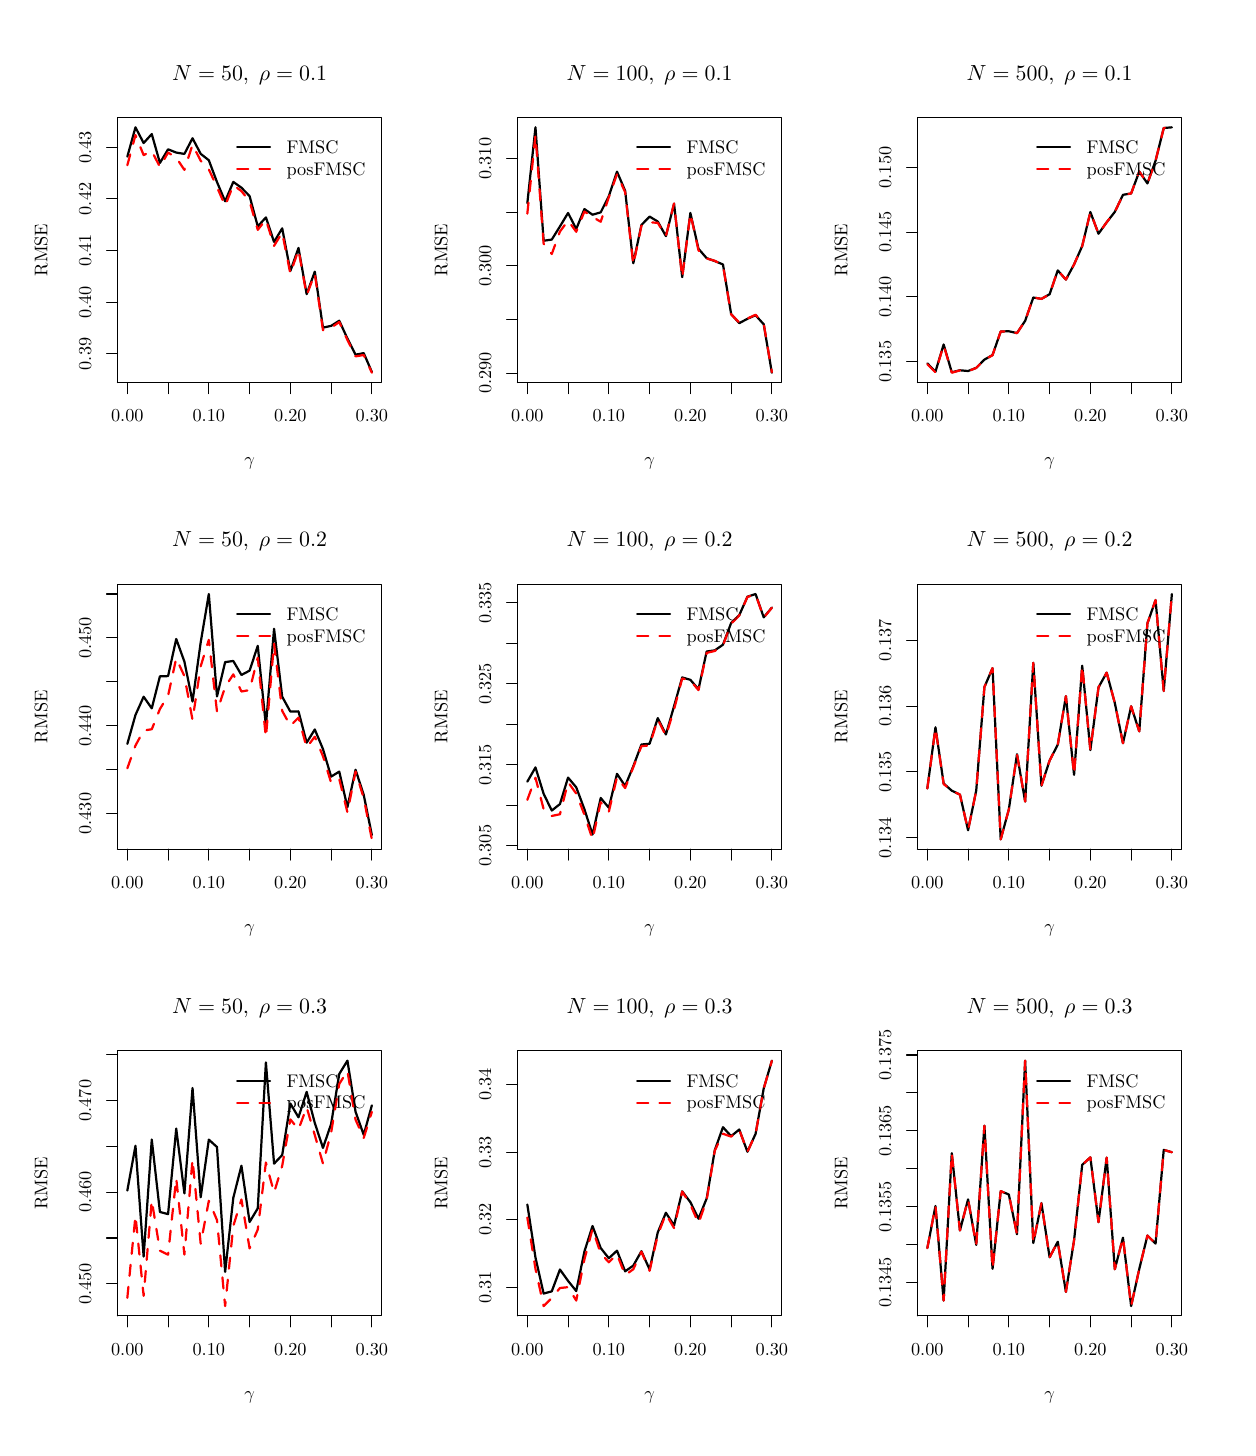
\begin{tikzpicture}[x=1pt,y=1pt]
\definecolor[named]{fillColor}{rgb}{1.00,1.00,1.00}
\path[use as bounding box,fill=fillColor,fill opacity=0.00] (0,0) rectangle (433.62,505.89);
\begin{scope}
\path[clip] ( 32.47,377.65) rectangle (127.91,473.42);
\definecolor[named]{drawColor}{rgb}{0.00,0.00,0.00}

\path[draw=drawColor,line width= 0.8pt,line join=round,line cap=round] ( 36.01,459.27) --
	( 38.95,469.87) --
	( 41.90,464.20) --
	( 44.84,467.44) --
	( 47.79,457.01) --
	( 50.73,461.94) --
	( 53.68,460.75) --
	( 56.63,460.27) --
	( 59.57,465.93) --
	( 62.52,460.29) --
	( 65.46,457.98) --
	( 68.41,450.10) --
	( 71.35,443.15) --
	( 74.30,450.15) --
	( 77.24,448.06) --
	( 80.19,445.03) --
	( 83.14,434.09) --
	( 86.08,437.32) --
	( 89.03,428.46) --
	( 91.97,433.38) --
	( 94.92,417.95) --
	( 97.86,426.29) --
	(100.81,409.59) --
	(103.75,417.72) --
	(106.70,397.48) --
	(109.65,398.14) --
	(112.59,399.99) --
	(115.54,393.54) --
	(118.48,387.71) --
	(121.43,388.29) --
	(124.37,381.47);
\end{scope}
\begin{scope}
\path[clip] (  0.00,  0.00) rectangle (433.62,505.89);
\definecolor[named]{drawColor}{rgb}{0.00,0.00,0.00}

\path[draw=drawColor,line width= 0.4pt,line join=round,line cap=round] ( 36.01,377.65) -- (124.37,377.65);

\path[draw=drawColor,line width= 0.4pt,line join=round,line cap=round] ( 36.01,377.65) -- ( 36.01,373.69);

\path[draw=drawColor,line width= 0.4pt,line join=round,line cap=round] ( 50.73,377.65) -- ( 50.73,373.69);

\path[draw=drawColor,line width= 0.4pt,line join=round,line cap=round] ( 65.46,377.65) -- ( 65.46,373.69);

\path[draw=drawColor,line width= 0.4pt,line join=round,line cap=round] ( 80.19,377.65) -- ( 80.19,373.69);

\path[draw=drawColor,line width= 0.4pt,line join=round,line cap=round] ( 94.92,377.65) -- ( 94.92,373.69);

\path[draw=drawColor,line width= 0.4pt,line join=round,line cap=round] (109.65,377.65) -- (109.65,373.69);

\path[draw=drawColor,line width= 0.4pt,line join=round,line cap=round] (124.37,377.65) -- (124.37,373.69);

\node[text=drawColor,anchor=base,inner sep=0pt, outer sep=0pt, scale=  0.66] at ( 36.01,363.40) {0.00};

\node[text=drawColor,anchor=base,inner sep=0pt, outer sep=0pt, scale=  0.66] at ( 65.46,363.40) {0.10};

\node[text=drawColor,anchor=base,inner sep=0pt, outer sep=0pt, scale=  0.66] at ( 94.92,363.40) {0.20};

\node[text=drawColor,anchor=base,inner sep=0pt, outer sep=0pt, scale=  0.66] at (124.37,363.40) {0.30};

\path[draw=drawColor,line width= 0.4pt,line join=round,line cap=round] ( 32.47,388.00) -- ( 32.47,462.68);

\path[draw=drawColor,line width= 0.4pt,line join=round,line cap=round] ( 32.47,388.00) -- ( 28.51,388.00);

\path[draw=drawColor,line width= 0.4pt,line join=round,line cap=round] ( 32.47,406.67) -- ( 28.51,406.67);

\path[draw=drawColor,line width= 0.4pt,line join=round,line cap=round] ( 32.47,425.34) -- ( 28.51,425.34);

\path[draw=drawColor,line width= 0.4pt,line join=round,line cap=round] ( 32.47,444.01) -- ( 28.51,444.01);

\path[draw=drawColor,line width= 0.4pt,line join=round,line cap=round] ( 32.47,462.68) -- ( 28.51,462.68);

\node[text=drawColor,rotate= 90.00,anchor=base,inner sep=0pt, outer sep=0pt, scale=  0.66] at ( 22.97,388.00) {0.39};

\node[text=drawColor,rotate= 90.00,anchor=base,inner sep=0pt, outer sep=0pt, scale=  0.66] at ( 22.97,406.67) {0.40};

\node[text=drawColor,rotate= 90.00,anchor=base,inner sep=0pt, outer sep=0pt, scale=  0.66] at ( 22.97,425.34) {0.41};

\node[text=drawColor,rotate= 90.00,anchor=base,inner sep=0pt, outer sep=0pt, scale=  0.66] at ( 22.97,444.01) {0.42};

\node[text=drawColor,rotate= 90.00,anchor=base,inner sep=0pt, outer sep=0pt, scale=  0.66] at ( 22.97,462.68) {0.43};

\path[draw=drawColor,line width= 0.4pt,line join=round,line cap=round] ( 32.47,377.65) --
	(127.91,377.65) --
	(127.91,473.42) --
	( 32.47,473.42) --
	( 32.47,377.65);
\end{scope}
\begin{scope}
\path[clip] (  0.00,337.26) rectangle (144.54,505.89);
\definecolor[named]{drawColor}{rgb}{0.00,0.00,0.00}

\node[text=drawColor,anchor=base,inner sep=0pt, outer sep=0pt, scale=  0.79] at ( 80.19,486.92) {\bfseries $N=50, \;\rho=0.1$};

\node[text=drawColor,anchor=base,inner sep=0pt, outer sep=0pt, scale=  0.66] at ( 80.19,347.56) {$\gamma$};

\node[text=drawColor,rotate= 90.00,anchor=base,inner sep=0pt, outer sep=0pt, scale=  0.66] at (  7.13,425.54) {RMSE};
\end{scope}
\begin{scope}
\path[clip] ( 32.47,377.65) rectangle (127.91,473.42);
\definecolor[named]{drawColor}{rgb}{1.00,0.00,0.00}

\path[draw=drawColor,line width= 0.8pt,dash pattern=on 4pt off 4pt ,line join=round,line cap=round] ( 36.01,456.18) --
	( 38.95,467.06) --
	( 41.90,459.85) --
	( 44.84,461.28) --
	( 47.79,455.56) --
	( 50.73,460.76) --
	( 53.68,458.93) --
	( 56.63,454.50) --
	( 59.57,463.59) --
	( 62.52,457.79) --
	( 65.46,454.67) --
	( 68.41,448.28) --
	( 71.35,441.53) --
	( 74.30,448.99) --
	( 77.24,446.83) --
	( 80.19,443.12) --
	( 83.14,432.82) --
	( 86.08,436.55) --
	( 89.03,427.06) --
	( 91.97,431.85) --
	( 94.92,416.97) --
	( 97.86,425.66) --
	(100.81,409.19) --
	(103.75,417.02) --
	(106.70,396.60) --
	(109.65,397.50) --
	(112.59,399.52) --
	(115.54,393.04) --
	(118.48,387.10) --
	(121.43,387.61) --
	(124.37,381.20);
\definecolor[named]{drawColor}{rgb}{0.00,0.00,0.00}

\path[draw=drawColor,line width= 0.8pt,line join=round,line cap=round] ( 75.72,462.63) -- ( 87.60,462.63);
\definecolor[named]{drawColor}{rgb}{1.00,0.00,0.00}

\path[draw=drawColor,line width= 0.8pt,dash pattern=on 4pt off 4pt ,line join=round,line cap=round] ( 75.72,454.71) -- ( 87.60,454.71);
\definecolor[named]{drawColor}{rgb}{0.00,0.00,0.00}

\node[text=drawColor,anchor=base west,inner sep=0pt, outer sep=0pt, scale=  0.66] at ( 93.54,460.35) {FMSC};

\node[text=drawColor,anchor=base west,inner sep=0pt, outer sep=0pt, scale=  0.66] at ( 93.54,452.43) {posFMSC};
\end{scope}
\begin{scope}
\path[clip] (177.01,377.65) rectangle (272.45,473.42);
\definecolor[named]{drawColor}{rgb}{0.00,0.00,0.00}

\path[draw=drawColor,line width= 0.8pt,line join=round,line cap=round] (180.55,442.46) --
	(183.49,469.87) --
	(186.44,428.89) --
	(189.38,429.31) --
	(192.33,434.06) --
	(195.27,438.93) --
	(198.22,433.14) --
	(201.17,440.34) --
	(204.11,438.30) --
	(207.06,439.15) --
	(210.00,445.04) --
	(212.95,453.86) --
	(215.89,446.96) --
	(218.84,420.75) --
	(221.78,434.60) --
	(224.73,437.62) --
	(227.68,435.83) --
	(230.62,430.56) --
	(233.57,442.29) --
	(236.51,415.74) --
	(239.46,438.94) --
	(242.40,425.98) --
	(245.35,422.59) --
	(248.29,421.55) --
	(251.24,420.32) --
	(254.19,402.42) --
	(257.13,399.11) --
	(260.08,400.69) --
	(263.02,401.97) --
	(265.97,398.70) --
	(268.91,381.20);
\end{scope}
\begin{scope}
\path[clip] (  0.00,  0.00) rectangle (433.62,505.89);
\definecolor[named]{drawColor}{rgb}{0.00,0.00,0.00}

\path[draw=drawColor,line width= 0.4pt,line join=round,line cap=round] (180.55,377.65) -- (268.91,377.65);

\path[draw=drawColor,line width= 0.4pt,line join=round,line cap=round] (180.55,377.65) -- (180.55,373.69);

\path[draw=drawColor,line width= 0.4pt,line join=round,line cap=round] (195.27,377.65) -- (195.27,373.69);

\path[draw=drawColor,line width= 0.4pt,line join=round,line cap=round] (210.00,377.65) -- (210.00,373.69);

\path[draw=drawColor,line width= 0.4pt,line join=round,line cap=round] (224.73,377.65) -- (224.73,373.69);

\path[draw=drawColor,line width= 0.4pt,line join=round,line cap=round] (239.46,377.65) -- (239.46,373.69);

\path[draw=drawColor,line width= 0.4pt,line join=round,line cap=round] (254.19,377.65) -- (254.19,373.69);

\path[draw=drawColor,line width= 0.4pt,line join=round,line cap=round] (268.91,377.65) -- (268.91,373.69);

\node[text=drawColor,anchor=base,inner sep=0pt, outer sep=0pt, scale=  0.66] at (180.55,363.40) {0.00};

\node[text=drawColor,anchor=base,inner sep=0pt, outer sep=0pt, scale=  0.66] at (210.00,363.40) {0.10};

\node[text=drawColor,anchor=base,inner sep=0pt, outer sep=0pt, scale=  0.66] at (239.46,363.40) {0.20};

\node[text=drawColor,anchor=base,inner sep=0pt, outer sep=0pt, scale=  0.66] at (268.91,363.40) {0.30};

\path[draw=drawColor,line width= 0.4pt,line join=round,line cap=round] (177.01,381.05) -- (177.01,458.57);

\path[draw=drawColor,line width= 0.4pt,line join=round,line cap=round] (177.01,381.05) -- (173.05,381.05);

\path[draw=drawColor,line width= 0.4pt,line join=round,line cap=round] (177.01,400.43) -- (173.05,400.43);

\path[draw=drawColor,line width= 0.4pt,line join=round,line cap=round] (177.01,419.81) -- (173.05,419.81);

\path[draw=drawColor,line width= 0.4pt,line join=round,line cap=round] (177.01,439.19) -- (173.05,439.19);

\path[draw=drawColor,line width= 0.4pt,line join=round,line cap=round] (177.01,458.57) -- (173.05,458.57);

\node[text=drawColor,rotate= 90.00,anchor=base,inner sep=0pt, outer sep=0pt, scale=  0.66] at (167.51,381.05) {0.290};

\node[text=drawColor,rotate= 90.00,anchor=base,inner sep=0pt, outer sep=0pt, scale=  0.66] at (167.51,419.81) {0.300};

\node[text=drawColor,rotate= 90.00,anchor=base,inner sep=0pt, outer sep=0pt, scale=  0.66] at (167.51,458.57) {0.310};

\path[draw=drawColor,line width= 0.4pt,line join=round,line cap=round] (177.01,377.65) --
	(272.45,377.65) --
	(272.45,473.42) --
	(177.01,473.42) --
	(177.01,377.65);
\end{scope}
\begin{scope}
\path[clip] (144.54,337.26) rectangle (289.08,505.89);
\definecolor[named]{drawColor}{rgb}{0.00,0.00,0.00}

\node[text=drawColor,anchor=base,inner sep=0pt, outer sep=0pt, scale=  0.79] at (224.73,486.92) {\bfseries $N=100, \;\rho=0.1$};

\node[text=drawColor,anchor=base,inner sep=0pt, outer sep=0pt, scale=  0.66] at (224.73,347.56) {$\gamma$};

\node[text=drawColor,rotate= 90.00,anchor=base,inner sep=0pt, outer sep=0pt, scale=  0.66] at (151.67,425.54) {RMSE};
\end{scope}
\begin{scope}
\path[clip] (177.01,377.65) rectangle (272.45,473.42);
\definecolor[named]{drawColor}{rgb}{1.00,0.00,0.00}

\path[draw=drawColor,line width= 0.8pt,dash pattern=on 4pt off 4pt ,line join=round,line cap=round] (180.55,438.68) --
	(183.49,466.99) --
	(186.44,427.83) --
	(189.38,424.10) --
	(192.33,432.21) --
	(195.27,436.17) --
	(198.22,432.14) --
	(201.17,439.45) --
	(204.11,437.50) --
	(207.06,435.75) --
	(210.00,444.63) --
	(212.95,452.94) --
	(215.89,446.45) --
	(218.84,420.26) --
	(221.78,434.26) --
	(224.73,435.53) --
	(227.68,435.37) --
	(230.62,430.60) --
	(233.57,442.36) --
	(236.51,415.60) --
	(239.46,438.74) --
	(242.40,425.39) --
	(245.35,422.49) --
	(248.29,421.64) --
	(251.24,420.05) --
	(254.19,402.29) --
	(257.13,399.33) --
	(260.08,400.78) --
	(263.02,402.15) --
	(265.97,398.93) --
	(268.91,381.38);
\definecolor[named]{drawColor}{rgb}{0.00,0.00,0.00}

\path[draw=drawColor,line width= 0.8pt,line join=round,line cap=round] (220.26,462.63) -- (232.14,462.63);
\definecolor[named]{drawColor}{rgb}{1.00,0.00,0.00}

\path[draw=drawColor,line width= 0.8pt,dash pattern=on 4pt off 4pt ,line join=round,line cap=round] (220.26,454.71) -- (232.14,454.71);
\definecolor[named]{drawColor}{rgb}{0.00,0.00,0.00}

\node[text=drawColor,anchor=base west,inner sep=0pt, outer sep=0pt, scale=  0.66] at (238.08,460.35) {FMSC};

\node[text=drawColor,anchor=base west,inner sep=0pt, outer sep=0pt, scale=  0.66] at (238.08,452.43) {posFMSC};
\end{scope}
\begin{scope}
\path[clip] (321.55,377.65) rectangle (416.99,473.42);
\definecolor[named]{drawColor}{rgb}{0.00,0.00,0.00}

\path[draw=drawColor,line width= 0.8pt,line join=round,line cap=round] (325.09,384.58) --
	(328.03,381.58) --
	(330.98,391.41) --
	(333.92,381.37) --
	(336.87,382.08) --
	(339.81,381.82) --
	(342.76,382.96) --
	(345.71,385.93) --
	(348.65,387.59) --
	(351.60,396.10) --
	(354.54,396.18) --
	(357.49,395.52) --
	(360.43,399.95) --
	(363.38,408.38) --
	(366.32,407.89) --
	(369.27,409.57) --
	(372.22,418.17) --
	(375.16,414.86) --
	(378.11,420.33) --
	(381.05,426.97) --
	(384.00,439.27) --
	(386.94,431.43) --
	(389.89,435.56) --
	(392.83,439.31) --
	(395.78,445.48) --
	(398.73,445.98) --
	(401.67,453.90) --
	(404.62,449.60) --
	(407.56,457.83) --
	(410.51,469.63) --
	(413.45,469.87);
\end{scope}
\begin{scope}
\path[clip] (  0.00,  0.00) rectangle (433.62,505.89);
\definecolor[named]{drawColor}{rgb}{0.00,0.00,0.00}

\path[draw=drawColor,line width= 0.4pt,line join=round,line cap=round] (325.09,377.65) -- (413.45,377.65);

\path[draw=drawColor,line width= 0.4pt,line join=round,line cap=round] (325.09,377.65) -- (325.09,373.69);

\path[draw=drawColor,line width= 0.4pt,line join=round,line cap=round] (339.81,377.65) -- (339.81,373.69);

\path[draw=drawColor,line width= 0.4pt,line join=round,line cap=round] (354.54,377.65) -- (354.54,373.69);

\path[draw=drawColor,line width= 0.4pt,line join=round,line cap=round] (369.27,377.65) -- (369.27,373.69);

\path[draw=drawColor,line width= 0.4pt,line join=round,line cap=round] (384.00,377.65) -- (384.00,373.69);

\path[draw=drawColor,line width= 0.4pt,line join=round,line cap=round] (398.73,377.65) -- (398.73,373.69);

\path[draw=drawColor,line width= 0.4pt,line join=round,line cap=round] (413.45,377.65) -- (413.45,373.69);

\node[text=drawColor,anchor=base,inner sep=0pt, outer sep=0pt, scale=  0.66] at (325.09,363.40) {0.00};

\node[text=drawColor,anchor=base,inner sep=0pt, outer sep=0pt, scale=  0.66] at (354.54,363.40) {0.10};

\node[text=drawColor,anchor=base,inner sep=0pt, outer sep=0pt, scale=  0.66] at (384.00,363.40) {0.20};

\node[text=drawColor,anchor=base,inner sep=0pt, outer sep=0pt, scale=  0.66] at (413.45,363.40) {0.30};

\path[draw=drawColor,line width= 0.4pt,line join=round,line cap=round] (321.55,385.24) -- (321.55,455.38);

\path[draw=drawColor,line width= 0.4pt,line join=round,line cap=round] (321.55,385.24) -- (317.59,385.24);

\path[draw=drawColor,line width= 0.4pt,line join=round,line cap=round] (321.55,408.62) -- (317.59,408.62);

\path[draw=drawColor,line width= 0.4pt,line join=round,line cap=round] (321.55,432.00) -- (317.59,432.00);

\path[draw=drawColor,line width= 0.4pt,line join=round,line cap=round] (321.55,455.38) -- (317.59,455.38);

\node[text=drawColor,rotate= 90.00,anchor=base,inner sep=0pt, outer sep=0pt, scale=  0.66] at (312.05,385.24) {0.135};

\node[text=drawColor,rotate= 90.00,anchor=base,inner sep=0pt, outer sep=0pt, scale=  0.66] at (312.05,408.62) {0.140};

\node[text=drawColor,rotate= 90.00,anchor=base,inner sep=0pt, outer sep=0pt, scale=  0.66] at (312.05,432.00) {0.145};

\node[text=drawColor,rotate= 90.00,anchor=base,inner sep=0pt, outer sep=0pt, scale=  0.66] at (312.05,455.38) {0.150};

\path[draw=drawColor,line width= 0.4pt,line join=round,line cap=round] (321.55,377.65) --
	(416.99,377.65) --
	(416.99,473.42) --
	(321.55,473.42) --
	(321.55,377.65);
\end{scope}
\begin{scope}
\path[clip] (289.08,337.26) rectangle (433.62,505.89);
\definecolor[named]{drawColor}{rgb}{0.00,0.00,0.00}

\node[text=drawColor,anchor=base,inner sep=0pt, outer sep=0pt, scale=  0.79] at (369.27,486.92) {\bfseries $N=500, \;\rho=0.1$};

\node[text=drawColor,anchor=base,inner sep=0pt, outer sep=0pt, scale=  0.66] at (369.27,347.56) {$\gamma$};

\node[text=drawColor,rotate= 90.00,anchor=base,inner sep=0pt, outer sep=0pt, scale=  0.66] at (296.21,425.53) {RMSE};
\end{scope}
\begin{scope}
\path[clip] (321.55,377.65) rectangle (416.99,473.42);
\definecolor[named]{drawColor}{rgb}{1.00,0.00,0.00}

\path[draw=drawColor,line width= 0.8pt,dash pattern=on 4pt off 4pt ,line join=round,line cap=round] (325.09,384.28) --
	(328.03,381.34) --
	(330.98,391.20) --
	(333.92,381.20) --
	(336.87,382.05) --
	(339.81,381.76) --
	(342.76,382.93) --
	(345.71,385.88) --
	(348.65,387.53) --
	(351.60,396.11) --
	(354.54,396.15) --
	(357.49,395.50) --
	(360.43,399.94) --
	(363.38,408.40) --
	(366.32,407.87) --
	(369.27,409.57) --
	(372.22,418.17) --
	(375.16,414.86) --
	(378.11,420.33) --
	(381.05,426.97) --
	(384.00,439.27) --
	(386.94,431.43) --
	(389.89,435.56) --
	(392.83,439.31) --
	(395.78,445.48) --
	(398.73,445.98) --
	(401.67,453.90) --
	(404.62,449.60) --
	(407.56,457.83) --
	(410.51,469.63) --
	(413.45,469.87);
\definecolor[named]{drawColor}{rgb}{0.00,0.00,0.00}

\path[draw=drawColor,line width= 0.8pt,line join=round,line cap=round] (364.80,462.63) -- (376.68,462.63);
\definecolor[named]{drawColor}{rgb}{1.00,0.00,0.00}

\path[draw=drawColor,line width= 0.8pt,dash pattern=on 4pt off 4pt ,line join=round,line cap=round] (364.80,454.71) -- (376.68,454.71);
\definecolor[named]{drawColor}{rgb}{0.00,0.00,0.00}

\node[text=drawColor,anchor=base west,inner sep=0pt, outer sep=0pt, scale=  0.66] at (382.62,460.35) {FMSC};

\node[text=drawColor,anchor=base west,inner sep=0pt, outer sep=0pt, scale=  0.66] at (382.62,452.43) {posFMSC};
\end{scope}
\begin{scope}
\path[clip] ( 32.47,209.02) rectangle (127.91,304.79);
\definecolor[named]{drawColor}{rgb}{0.00,0.00,0.00}

\path[draw=drawColor,line width= 0.8pt,line join=round,line cap=round] ( 36.01,247.07) --
	( 38.95,257.52) --
	( 41.90,264.12) --
	( 44.84,259.92) --
	( 47.79,271.51) --
	( 50.73,271.57) --
	( 53.68,284.99) --
	( 56.63,276.83) --
	( 59.57,262.37) --
	( 62.52,283.78) --
	( 65.46,301.24) --
	( 68.41,264.22) --
	( 71.35,276.63) --
	( 74.30,277.05) --
	( 77.24,271.99) --
	( 80.19,273.55) --
	( 83.14,282.53) --
	( 86.08,253.66) --
	( 89.03,288.68) --
	( 91.97,264.13) --
	( 94.92,258.75) --
	( 97.86,258.84) --
	(100.81,247.53) --
	(103.75,252.30) --
	(106.70,245.23) --
	(109.65,235.25) --
	(112.59,237.07) --
	(115.54,224.21) --
	(118.48,237.74) --
	(121.43,228.67) --
	(124.37,214.16);
\end{scope}
\begin{scope}
\path[clip] (  0.00,  0.00) rectangle (433.62,505.89);
\definecolor[named]{drawColor}{rgb}{0.00,0.00,0.00}

\path[draw=drawColor,line width= 0.4pt,line join=round,line cap=round] ( 36.01,209.02) -- (124.37,209.02);

\path[draw=drawColor,line width= 0.4pt,line join=round,line cap=round] ( 36.01,209.02) -- ( 36.01,205.06);

\path[draw=drawColor,line width= 0.4pt,line join=round,line cap=round] ( 50.73,209.02) -- ( 50.73,205.06);

\path[draw=drawColor,line width= 0.4pt,line join=round,line cap=round] ( 65.46,209.02) -- ( 65.46,205.06);

\path[draw=drawColor,line width= 0.4pt,line join=round,line cap=round] ( 80.19,209.02) -- ( 80.19,205.06);

\path[draw=drawColor,line width= 0.4pt,line join=round,line cap=round] ( 94.92,209.02) -- ( 94.92,205.06);

\path[draw=drawColor,line width= 0.4pt,line join=round,line cap=round] (109.65,209.02) -- (109.65,205.06);

\path[draw=drawColor,line width= 0.4pt,line join=round,line cap=round] (124.37,209.02) -- (124.37,205.06);

\node[text=drawColor,anchor=base,inner sep=0pt, outer sep=0pt, scale=  0.66] at ( 36.01,194.77) {0.00};

\node[text=drawColor,anchor=base,inner sep=0pt, outer sep=0pt, scale=  0.66] at ( 65.46,194.77) {0.10};

\node[text=drawColor,anchor=base,inner sep=0pt, outer sep=0pt, scale=  0.66] at ( 94.92,194.77) {0.20};

\node[text=drawColor,anchor=base,inner sep=0pt, outer sep=0pt, scale=  0.66] at (124.37,194.77) {0.30};

\path[draw=drawColor,line width= 0.4pt,line join=round,line cap=round] ( 32.47,221.88) -- ( 32.47,301.26);

\path[draw=drawColor,line width= 0.4pt,line join=round,line cap=round] ( 32.47,221.88) -- ( 28.51,221.88);

\path[draw=drawColor,line width= 0.4pt,line join=round,line cap=round] ( 32.47,237.76) -- ( 28.51,237.76);

\path[draw=drawColor,line width= 0.4pt,line join=round,line cap=round] ( 32.47,253.63) -- ( 28.51,253.63);

\path[draw=drawColor,line width= 0.4pt,line join=round,line cap=round] ( 32.47,269.51) -- ( 28.51,269.51);

\path[draw=drawColor,line width= 0.4pt,line join=round,line cap=round] ( 32.47,285.38) -- ( 28.51,285.38);

\path[draw=drawColor,line width= 0.4pt,line join=round,line cap=round] ( 32.47,301.26) -- ( 28.51,301.26);

\node[text=drawColor,rotate= 90.00,anchor=base,inner sep=0pt, outer sep=0pt, scale=  0.66] at ( 22.97,221.88) {0.430};

\node[text=drawColor,rotate= 90.00,anchor=base,inner sep=0pt, outer sep=0pt, scale=  0.66] at ( 22.97,253.63) {0.440};

\node[text=drawColor,rotate= 90.00,anchor=base,inner sep=0pt, outer sep=0pt, scale=  0.66] at ( 22.97,285.38) {0.450};

\path[draw=drawColor,line width= 0.4pt,line join=round,line cap=round] ( 32.47,209.02) --
	(127.91,209.02) --
	(127.91,304.79) --
	( 32.47,304.79) --
	( 32.47,209.02);
\end{scope}
\begin{scope}
\path[clip] (  0.00,168.63) rectangle (144.54,337.26);
\definecolor[named]{drawColor}{rgb}{0.00,0.00,0.00}

\node[text=drawColor,anchor=base,inner sep=0pt, outer sep=0pt, scale=  0.79] at ( 80.19,318.29) {\bfseries $N=50, \;\rho=0.2$};

\node[text=drawColor,anchor=base,inner sep=0pt, outer sep=0pt, scale=  0.66] at ( 80.19,178.93) {$\gamma$};

\node[text=drawColor,rotate= 90.00,anchor=base,inner sep=0pt, outer sep=0pt, scale=  0.66] at (  7.13,256.90) {RMSE};
\end{scope}
\begin{scope}
\path[clip] ( 32.47,209.02) rectangle (127.91,304.79);
\definecolor[named]{drawColor}{rgb}{1.00,0.00,0.00}

\path[draw=drawColor,line width= 0.8pt,dash pattern=on 4pt off 4pt ,line join=round,line cap=round] ( 36.01,238.26) --
	( 38.95,246.48) --
	( 41.90,251.92) --
	( 44.84,252.37) --
	( 47.79,259.69) --
	( 50.73,264.49) --
	( 53.68,278.00) --
	( 56.63,271.58) --
	( 59.57,255.75) --
	( 62.52,275.14) --
	( 65.46,284.69) --
	( 68.41,258.73) --
	( 71.35,267.65) --
	( 74.30,272.21) --
	( 77.24,266.02) --
	( 80.19,266.52) --
	( 83.14,278.22) --
	( 86.08,249.41) --
	( 89.03,283.37) --
	( 91.97,259.02) --
	( 94.92,253.60) --
	( 97.86,256.58) --
	(100.81,245.77) --
	(103.75,249.69) --
	(106.70,242.66) --
	(109.65,233.06) --
	(112.59,234.38) --
	(115.54,222.36) --
	(118.48,237.10) --
	(121.43,227.51) --
	(124.37,212.57);
\definecolor[named]{drawColor}{rgb}{0.00,0.00,0.00}

\path[draw=drawColor,line width= 0.8pt,line join=round,line cap=round] ( 75.72,294.00) -- ( 87.60,294.00);
\definecolor[named]{drawColor}{rgb}{1.00,0.00,0.00}

\path[draw=drawColor,line width= 0.8pt,dash pattern=on 4pt off 4pt ,line join=round,line cap=round] ( 75.72,286.08) -- ( 87.60,286.08);
\definecolor[named]{drawColor}{rgb}{0.00,0.00,0.00}

\node[text=drawColor,anchor=base west,inner sep=0pt, outer sep=0pt, scale=  0.66] at ( 93.54,291.72) {FMSC};

\node[text=drawColor,anchor=base west,inner sep=0pt, outer sep=0pt, scale=  0.66] at ( 93.54,283.80) {posFMSC};
\end{scope}
\begin{scope}
\path[clip] (177.01,209.02) rectangle (272.45,304.79);
\definecolor[named]{drawColor}{rgb}{0.00,0.00,0.00}

\path[draw=drawColor,line width= 0.8pt,line join=round,line cap=round] (180.55,233.44) --
	(183.49,238.58) --
	(186.44,229.06) --
	(189.38,222.99) --
	(192.33,225.33) --
	(195.27,234.91) --
	(198.22,231.38) --
	(201.17,223.50) --
	(204.11,214.31) --
	(207.06,227.54) --
	(210.00,224.01) --
	(212.95,236.27) --
	(215.89,231.87) --
	(218.84,239.00) --
	(221.78,246.85) --
	(224.73,247.14) --
	(227.68,256.39) --
	(230.62,250.48) --
	(233.57,260.71) --
	(236.51,271.09) --
	(239.46,270.24) --
	(242.40,266.82) --
	(245.35,280.47) --
	(248.29,280.88) --
	(251.24,282.91) --
	(254.19,290.77) --
	(257.13,293.60) --
	(260.08,300.26) --
	(263.02,301.24) --
	(265.97,292.81) --
	(268.91,296.35);
\end{scope}
\begin{scope}
\path[clip] (  0.00,  0.00) rectangle (433.62,505.89);
\definecolor[named]{drawColor}{rgb}{0.00,0.00,0.00}

\path[draw=drawColor,line width= 0.4pt,line join=round,line cap=round] (180.55,209.02) -- (268.91,209.02);

\path[draw=drawColor,line width= 0.4pt,line join=round,line cap=round] (180.55,209.02) -- (180.55,205.06);

\path[draw=drawColor,line width= 0.4pt,line join=round,line cap=round] (195.27,209.02) -- (195.27,205.06);

\path[draw=drawColor,line width= 0.4pt,line join=round,line cap=round] (210.00,209.02) -- (210.00,205.06);

\path[draw=drawColor,line width= 0.4pt,line join=round,line cap=round] (224.73,209.02) -- (224.73,205.06);

\path[draw=drawColor,line width= 0.4pt,line join=round,line cap=round] (239.46,209.02) -- (239.46,205.06);

\path[draw=drawColor,line width= 0.4pt,line join=round,line cap=round] (254.19,209.02) -- (254.19,205.06);

\path[draw=drawColor,line width= 0.4pt,line join=round,line cap=round] (268.91,209.02) -- (268.91,205.06);

\node[text=drawColor,anchor=base,inner sep=0pt, outer sep=0pt, scale=  0.66] at (180.55,194.77) {0.00};

\node[text=drawColor,anchor=base,inner sep=0pt, outer sep=0pt, scale=  0.66] at (210.00,194.77) {0.10};

\node[text=drawColor,anchor=base,inner sep=0pt, outer sep=0pt, scale=  0.66] at (239.46,194.77) {0.20};

\node[text=drawColor,anchor=base,inner sep=0pt, outer sep=0pt, scale=  0.66] at (268.91,194.77) {0.30};

\path[draw=drawColor,line width= 0.4pt,line join=round,line cap=round] (177.01,210.31) -- (177.01,298.05);

\path[draw=drawColor,line width= 0.4pt,line join=round,line cap=round] (177.01,210.31) -- (173.05,210.31);

\path[draw=drawColor,line width= 0.4pt,line join=round,line cap=round] (177.01,224.93) -- (173.05,224.93);

\path[draw=drawColor,line width= 0.4pt,line join=round,line cap=round] (177.01,239.56) -- (173.05,239.56);

\path[draw=drawColor,line width= 0.4pt,line join=round,line cap=round] (177.01,254.18) -- (173.05,254.18);

\path[draw=drawColor,line width= 0.4pt,line join=round,line cap=round] (177.01,268.80) -- (173.05,268.80);

\path[draw=drawColor,line width= 0.4pt,line join=round,line cap=round] (177.01,283.43) -- (173.05,283.43);

\path[draw=drawColor,line width= 0.4pt,line join=round,line cap=round] (177.01,298.05) -- (173.05,298.05);

\node[text=drawColor,rotate= 90.00,anchor=base,inner sep=0pt, outer sep=0pt, scale=  0.66] at (167.51,210.31) {0.305};

\node[text=drawColor,rotate= 90.00,anchor=base,inner sep=0pt, outer sep=0pt, scale=  0.66] at (167.51,239.56) {0.315};

\node[text=drawColor,rotate= 90.00,anchor=base,inner sep=0pt, outer sep=0pt, scale=  0.66] at (167.51,268.80) {0.325};

\node[text=drawColor,rotate= 90.00,anchor=base,inner sep=0pt, outer sep=0pt, scale=  0.66] at (167.51,298.05) {0.335};

\path[draw=drawColor,line width= 0.4pt,line join=round,line cap=round] (177.01,209.02) --
	(272.45,209.02) --
	(272.45,304.79) --
	(177.01,304.79) --
	(177.01,209.02);
\end{scope}
\begin{scope}
\path[clip] (144.54,168.63) rectangle (289.08,337.26);
\definecolor[named]{drawColor}{rgb}{0.00,0.00,0.00}

\node[text=drawColor,anchor=base,inner sep=0pt, outer sep=0pt, scale=  0.79] at (224.73,318.29) {\bfseries $N=100, \;\rho=0.2$};

\node[text=drawColor,anchor=base,inner sep=0pt, outer sep=0pt, scale=  0.66] at (224.73,178.93) {$\gamma$};

\node[text=drawColor,rotate= 90.00,anchor=base,inner sep=0pt, outer sep=0pt, scale=  0.66] at (151.67,256.91) {RMSE};
\end{scope}
\begin{scope}
\path[clip] (177.01,209.02) rectangle (272.45,304.79);
\definecolor[named]{drawColor}{rgb}{1.00,0.00,0.00}

\path[draw=drawColor,line width= 0.8pt,dash pattern=on 4pt off 4pt ,line join=round,line cap=round] (180.55,226.86) --
	(183.49,234.85) --
	(186.44,223.50) --
	(189.38,221.05) --
	(192.33,221.65) --
	(195.27,233.24) --
	(198.22,229.13) --
	(201.17,221.53) --
	(204.11,212.57) --
	(207.06,226.00) --
	(210.00,222.58) --
	(212.95,235.08) --
	(215.89,231.12) --
	(218.84,238.67) --
	(221.78,246.26) --
	(224.73,246.53) --
	(227.68,255.98) --
	(230.62,249.98) --
	(233.57,259.55) --
	(236.51,270.72) --
	(239.46,270.00) --
	(242.40,266.50) --
	(245.35,279.96) --
	(248.29,280.66) --
	(251.24,282.62) --
	(254.19,290.56) --
	(257.13,293.48) --
	(260.08,300.17) --
	(263.02,301.13) --
	(265.97,292.66) --
	(268.91,296.27);
\definecolor[named]{drawColor}{rgb}{0.00,0.00,0.00}

\path[draw=drawColor,line width= 0.8pt,line join=round,line cap=round] (220.26,294.00) -- (232.14,294.00);
\definecolor[named]{drawColor}{rgb}{1.00,0.00,0.00}

\path[draw=drawColor,line width= 0.8pt,dash pattern=on 4pt off 4pt ,line join=round,line cap=round] (220.26,286.08) -- (232.14,286.08);
\definecolor[named]{drawColor}{rgb}{0.00,0.00,0.00}

\node[text=drawColor,anchor=base west,inner sep=0pt, outer sep=0pt, scale=  0.66] at (238.08,291.72) {FMSC};

\node[text=drawColor,anchor=base west,inner sep=0pt, outer sep=0pt, scale=  0.66] at (238.08,283.80) {posFMSC};
\end{scope}
\begin{scope}
\path[clip] (321.55,209.02) rectangle (416.99,304.79);
\definecolor[named]{drawColor}{rgb}{0.00,0.00,0.00}

\path[draw=drawColor,line width= 0.8pt,line join=round,line cap=round] (325.09,230.99) --
	(328.03,253.08) --
	(330.98,232.77) --
	(333.92,230.18) --
	(336.87,228.76) --
	(339.81,215.88) --
	(342.76,230.26) --
	(345.71,267.60) --
	(348.65,274.47) --
	(351.60,212.57) --
	(354.54,223.42) --
	(357.49,243.36) --
	(360.43,226.26) --
	(363.38,276.37) --
	(366.32,231.96) --
	(369.27,241.07) --
	(372.22,246.79) --
	(375.16,264.33) --
	(378.11,235.91) --
	(381.05,275.34) --
	(384.00,244.83) --
	(386.94,267.52) --
	(389.89,272.83) --
	(392.83,261.88) --
	(395.78,247.32) --
	(398.73,260.66) --
	(401.67,251.61) --
	(404.62,290.64) --
	(407.56,299.06) --
	(410.51,266.22) --
	(413.45,301.24);
\end{scope}
\begin{scope}
\path[clip] (  0.00,  0.00) rectangle (433.62,505.89);
\definecolor[named]{drawColor}{rgb}{0.00,0.00,0.00}

\path[draw=drawColor,line width= 0.4pt,line join=round,line cap=round] (325.09,209.02) -- (413.45,209.02);

\path[draw=drawColor,line width= 0.4pt,line join=round,line cap=round] (325.09,209.02) -- (325.09,205.06);

\path[draw=drawColor,line width= 0.4pt,line join=round,line cap=round] (339.81,209.02) -- (339.81,205.06);

\path[draw=drawColor,line width= 0.4pt,line join=round,line cap=round] (354.54,209.02) -- (354.54,205.06);

\path[draw=drawColor,line width= 0.4pt,line join=round,line cap=round] (369.27,209.02) -- (369.27,205.06);

\path[draw=drawColor,line width= 0.4pt,line join=round,line cap=round] (384.00,209.02) -- (384.00,205.06);

\path[draw=drawColor,line width= 0.4pt,line join=round,line cap=round] (398.73,209.02) -- (398.73,205.06);

\path[draw=drawColor,line width= 0.4pt,line join=round,line cap=round] (413.45,209.02) -- (413.45,205.06);

\node[text=drawColor,anchor=base,inner sep=0pt, outer sep=0pt, scale=  0.66] at (325.09,194.77) {0.00};

\node[text=drawColor,anchor=base,inner sep=0pt, outer sep=0pt, scale=  0.66] at (354.54,194.77) {0.10};

\node[text=drawColor,anchor=base,inner sep=0pt, outer sep=0pt, scale=  0.66] at (384.00,194.77) {0.20};

\node[text=drawColor,anchor=base,inner sep=0pt, outer sep=0pt, scale=  0.66] at (413.45,194.77) {0.30};

\path[draw=drawColor,line width= 0.4pt,line join=round,line cap=round] (321.55,213.15) -- (321.55,284.54);

\path[draw=drawColor,line width= 0.4pt,line join=round,line cap=round] (321.55,213.15) -- (317.59,213.15);

\path[draw=drawColor,line width= 0.4pt,line join=round,line cap=round] (321.55,236.95) -- (317.59,236.95);

\path[draw=drawColor,line width= 0.4pt,line join=round,line cap=round] (321.55,260.74) -- (317.59,260.74);

\path[draw=drawColor,line width= 0.4pt,line join=round,line cap=round] (321.55,284.54) -- (317.59,284.54);

\node[text=drawColor,rotate= 90.00,anchor=base,inner sep=0pt, outer sep=0pt, scale=  0.66] at (312.05,213.15) {0.134};

\node[text=drawColor,rotate= 90.00,anchor=base,inner sep=0pt, outer sep=0pt, scale=  0.66] at (312.05,236.95) {0.135};

\node[text=drawColor,rotate= 90.00,anchor=base,inner sep=0pt, outer sep=0pt, scale=  0.66] at (312.05,260.74) {0.136};

\node[text=drawColor,rotate= 90.00,anchor=base,inner sep=0pt, outer sep=0pt, scale=  0.66] at (312.05,284.54) {0.137};

\path[draw=drawColor,line width= 0.4pt,line join=round,line cap=round] (321.55,209.02) --
	(416.99,209.02) --
	(416.99,304.79) --
	(321.55,304.79) --
	(321.55,209.02);
\end{scope}
\begin{scope}
\path[clip] (289.08,168.63) rectangle (433.62,337.26);
\definecolor[named]{drawColor}{rgb}{0.00,0.00,0.00}

\node[text=drawColor,anchor=base,inner sep=0pt, outer sep=0pt, scale=  0.79] at (369.27,318.29) {\bfseries $N=500, \;\rho=0.2$};

\node[text=drawColor,anchor=base,inner sep=0pt, outer sep=0pt, scale=  0.66] at (369.27,178.93) {$\gamma$};

\node[text=drawColor,rotate= 90.00,anchor=base,inner sep=0pt, outer sep=0pt, scale=  0.66] at (296.21,256.90) {RMSE};
\end{scope}
\begin{scope}
\path[clip] (321.55,209.02) rectangle (416.99,304.79);
\definecolor[named]{drawColor}{rgb}{1.00,0.00,0.00}

\path[draw=drawColor,line width= 0.8pt,dash pattern=on 4pt off 4pt ,line join=round,line cap=round] (325.09,230.99) --
	(328.03,252.82) --
	(330.98,232.57) --
	(333.92,230.18) --
	(336.87,228.75) --
	(339.81,215.88) --
	(342.76,230.21) --
	(345.71,267.60) --
	(348.65,274.47) --
	(351.60,212.57) --
	(354.54,223.42) --
	(357.49,243.36) --
	(360.43,226.26) --
	(363.38,276.37) --
	(366.32,231.96) --
	(369.27,241.07) --
	(372.22,246.78) --
	(375.16,264.33) --
	(378.11,235.91) --
	(381.05,275.34) --
	(384.00,244.83) --
	(386.94,267.52) --
	(389.89,272.83) --
	(392.83,261.88) --
	(395.78,247.32) --
	(398.73,260.66) --
	(401.67,251.61) --
	(404.62,290.64) --
	(407.56,299.06) --
	(410.51,266.22) --
	(413.45,301.24);
\definecolor[named]{drawColor}{rgb}{0.00,0.00,0.00}

\path[draw=drawColor,line width= 0.8pt,line join=round,line cap=round] (364.80,294.00) -- (376.68,294.00);
\definecolor[named]{drawColor}{rgb}{1.00,0.00,0.00}

\path[draw=drawColor,line width= 0.8pt,dash pattern=on 4pt off 4pt ,line join=round,line cap=round] (364.80,286.08) -- (376.68,286.08);
\definecolor[named]{drawColor}{rgb}{0.00,0.00,0.00}

\node[text=drawColor,anchor=base west,inner sep=0pt, outer sep=0pt, scale=  0.66] at (382.62,291.72) {FMSC};

\node[text=drawColor,anchor=base west,inner sep=0pt, outer sep=0pt, scale=  0.66] at (382.62,283.80) {posFMSC};
\end{scope}
\begin{scope}
\path[clip] ( 32.47, 40.39) rectangle (127.91,136.16);
\definecolor[named]{drawColor}{rgb}{0.00,0.00,0.00}

\path[draw=drawColor,line width= 0.8pt,line join=round,line cap=round] ( 36.01, 85.67) --
	( 38.95,101.87) --
	( 41.90, 61.83) --
	( 44.84,104.10) --
	( 47.79, 77.94) --
	( 50.73, 77.17) --
	( 53.68,108.07) --
	( 56.63, 84.64) --
	( 59.57,122.75) --
	( 62.52, 83.25) --
	( 65.46,104.08) --
	( 68.41,101.41) --
	( 71.35, 56.27) --
	( 74.30, 83.04) --
	( 77.24, 94.67) --
	( 80.19, 74.33) --
	( 83.14, 79.25) --
	( 86.08,131.97) --
	( 89.03, 95.39) --
	( 91.97, 98.51) --
	( 94.92,117.13) --
	( 97.86,112.15) --
	(100.81,121.34) --
	(103.75,110.09) --
	(106.70,101.09) --
	(109.65,109.74) --
	(112.59,127.82) --
	(115.54,132.61) --
	(118.48,114.15) --
	(121.43,105.81) --
	(124.37,116.46);
\end{scope}
\begin{scope}
\path[clip] (  0.00,  0.00) rectangle (433.62,505.89);
\definecolor[named]{drawColor}{rgb}{0.00,0.00,0.00}

\path[draw=drawColor,line width= 0.4pt,line join=round,line cap=round] ( 36.01, 40.39) -- (124.37, 40.39);

\path[draw=drawColor,line width= 0.4pt,line join=round,line cap=round] ( 36.01, 40.39) -- ( 36.01, 36.43);

\path[draw=drawColor,line width= 0.4pt,line join=round,line cap=round] ( 50.73, 40.39) -- ( 50.73, 36.43);

\path[draw=drawColor,line width= 0.4pt,line join=round,line cap=round] ( 65.46, 40.39) -- ( 65.46, 36.43);

\path[draw=drawColor,line width= 0.4pt,line join=round,line cap=round] ( 80.19, 40.39) -- ( 80.19, 36.43);

\path[draw=drawColor,line width= 0.4pt,line join=round,line cap=round] ( 94.92, 40.39) -- ( 94.92, 36.43);

\path[draw=drawColor,line width= 0.4pt,line join=round,line cap=round] (109.65, 40.39) -- (109.65, 36.43);

\path[draw=drawColor,line width= 0.4pt,line join=round,line cap=round] (124.37, 40.39) -- (124.37, 36.43);

\node[text=drawColor,anchor=base,inner sep=0pt, outer sep=0pt, scale=  0.66] at ( 36.01, 26.14) {0.00};

\node[text=drawColor,anchor=base,inner sep=0pt, outer sep=0pt, scale=  0.66] at ( 65.46, 26.14) {0.10};

\node[text=drawColor,anchor=base,inner sep=0pt, outer sep=0pt, scale=  0.66] at ( 94.92, 26.14) {0.20};

\node[text=drawColor,anchor=base,inner sep=0pt, outer sep=0pt, scale=  0.66] at (124.37, 26.14) {0.30};

\path[draw=drawColor,line width= 0.4pt,line join=round,line cap=round] ( 32.47, 51.96) -- ( 32.47,134.78);

\path[draw=drawColor,line width= 0.4pt,line join=round,line cap=round] ( 32.47, 51.96) -- ( 28.51, 51.96);

\path[draw=drawColor,line width= 0.4pt,line join=round,line cap=round] ( 32.47, 68.53) -- ( 28.51, 68.53);

\path[draw=drawColor,line width= 0.4pt,line join=round,line cap=round] ( 32.47, 85.09) -- ( 28.51, 85.09);

\path[draw=drawColor,line width= 0.4pt,line join=round,line cap=round] ( 32.47,101.65) -- ( 28.51,101.65);

\path[draw=drawColor,line width= 0.4pt,line join=round,line cap=round] ( 32.47,118.21) -- ( 28.51,118.21);

\path[draw=drawColor,line width= 0.4pt,line join=round,line cap=round] ( 32.47,134.78) -- ( 28.51,134.78);

\node[text=drawColor,rotate= 90.00,anchor=base,inner sep=0pt, outer sep=0pt, scale=  0.66] at ( 22.97, 51.96) {0.450};

\node[text=drawColor,rotate= 90.00,anchor=base,inner sep=0pt, outer sep=0pt, scale=  0.66] at ( 22.97, 85.09) {0.460};

\node[text=drawColor,rotate= 90.00,anchor=base,inner sep=0pt, outer sep=0pt, scale=  0.66] at ( 22.97,118.21) {0.470};

\path[draw=drawColor,line width= 0.4pt,line join=round,line cap=round] ( 32.47, 40.39) --
	(127.91, 40.39) --
	(127.91,136.16) --
	( 32.47,136.16) --
	( 32.47, 40.39);
\end{scope}
\begin{scope}
\path[clip] (  0.00,  0.00) rectangle (144.54,168.63);
\definecolor[named]{drawColor}{rgb}{0.00,0.00,0.00}

\node[text=drawColor,anchor=base,inner sep=0pt, outer sep=0pt, scale=  0.79] at ( 80.19,149.66) {\bfseries $N=50, \;\rho=0.3$};

\node[text=drawColor,anchor=base,inner sep=0pt, outer sep=0pt, scale=  0.66] at ( 80.19, 10.30) {$\gamma$};

\node[text=drawColor,rotate= 90.00,anchor=base,inner sep=0pt, outer sep=0pt, scale=  0.66] at (  7.13, 88.27) {RMSE};
\end{scope}
\begin{scope}
\path[clip] ( 32.47, 40.39) rectangle (127.91,136.16);
\definecolor[named]{drawColor}{rgb}{1.00,0.00,0.00}

\path[draw=drawColor,line width= 0.8pt,dash pattern=on 4pt off 4pt ,line join=round,line cap=round] ( 36.01, 46.91) --
	( 38.95, 76.62) --
	( 41.90, 47.65) --
	( 44.84, 82.13) --
	( 47.79, 63.96) --
	( 50.73, 62.50) --
	( 53.68, 90.13) --
	( 56.63, 62.55) --
	( 59.57, 96.92) --
	( 62.52, 66.48) --
	( 65.46, 81.97) --
	( 68.41, 75.01) --
	( 71.35, 43.94) --
	( 74.30, 72.85) --
	( 77.24, 82.45) --
	( 80.19, 64.79) --
	( 83.14, 71.58) --
	( 86.08, 95.81) --
	( 89.03, 84.93) --
	( 91.97, 94.61) --
	( 94.92,111.41) --
	( 97.86,107.76) --
	(100.81,115.78) --
	(103.75,105.72) --
	(106.70, 95.47) --
	(109.65,106.62) --
	(112.59,124.21) --
	(115.54,128.89) --
	(118.48,111.28) --
	(121.43,104.71) --
	(124.37,114.12);
\definecolor[named]{drawColor}{rgb}{0.00,0.00,0.00}

\path[draw=drawColor,line width= 0.8pt,line join=round,line cap=round] ( 75.72,125.37) -- ( 87.60,125.37);
\definecolor[named]{drawColor}{rgb}{1.00,0.00,0.00}

\path[draw=drawColor,line width= 0.8pt,dash pattern=on 4pt off 4pt ,line join=round,line cap=round] ( 75.72,117.45) -- ( 87.60,117.45);
\definecolor[named]{drawColor}{rgb}{0.00,0.00,0.00}

\node[text=drawColor,anchor=base west,inner sep=0pt, outer sep=0pt, scale=  0.66] at ( 93.54,123.09) {FMSC};

\node[text=drawColor,anchor=base west,inner sep=0pt, outer sep=0pt, scale=  0.66] at ( 93.54,115.17) {posFMSC};
\end{scope}
\begin{scope}
\path[clip] (177.01, 40.39) rectangle (272.45,136.16);
\definecolor[named]{drawColor}{rgb}{0.00,0.00,0.00}

\path[draw=drawColor,line width= 0.8pt,line join=round,line cap=round] (180.55, 80.62) --
	(183.49, 61.48) --
	(186.44, 48.46) --
	(189.38, 49.26) --
	(192.33, 57.15) --
	(195.27, 53.04) --
	(198.22, 49.37) --
	(201.17, 63.63) --
	(204.11, 72.88) --
	(207.06, 64.92) --
	(210.00, 61.22) --
	(212.95, 63.96) --
	(215.89, 56.50) --
	(218.84, 58.56) --
	(221.78, 63.77) --
	(224.73, 57.16) --
	(227.68, 70.56) --
	(230.62, 77.66) --
	(233.57, 73.06) --
	(236.51, 85.40) --
	(239.46, 81.49) --
	(242.40, 75.52) --
	(245.35, 82.82) --
	(248.29,100.28) --
	(251.24,108.58) --
	(254.19,105.34) --
	(257.13,107.73) --
	(260.08, 99.71) --
	(263.02,106.16) --
	(265.97,122.59) --
	(268.91,132.61);
\end{scope}
\begin{scope}
\path[clip] (  0.00,  0.00) rectangle (433.62,505.89);
\definecolor[named]{drawColor}{rgb}{0.00,0.00,0.00}

\path[draw=drawColor,line width= 0.4pt,line join=round,line cap=round] (180.55, 40.39) -- (268.91, 40.39);

\path[draw=drawColor,line width= 0.4pt,line join=round,line cap=round] (180.55, 40.39) -- (180.55, 36.43);

\path[draw=drawColor,line width= 0.4pt,line join=round,line cap=round] (195.27, 40.39) -- (195.27, 36.43);

\path[draw=drawColor,line width= 0.4pt,line join=round,line cap=round] (210.00, 40.39) -- (210.00, 36.43);

\path[draw=drawColor,line width= 0.4pt,line join=round,line cap=round] (224.73, 40.39) -- (224.73, 36.43);

\path[draw=drawColor,line width= 0.4pt,line join=round,line cap=round] (239.46, 40.39) -- (239.46, 36.43);

\path[draw=drawColor,line width= 0.4pt,line join=round,line cap=round] (254.19, 40.39) -- (254.19, 36.43);

\path[draw=drawColor,line width= 0.4pt,line join=round,line cap=round] (268.91, 40.39) -- (268.91, 36.43);

\node[text=drawColor,anchor=base,inner sep=0pt, outer sep=0pt, scale=  0.66] at (180.55, 26.14) {0.00};

\node[text=drawColor,anchor=base,inner sep=0pt, outer sep=0pt, scale=  0.66] at (210.00, 26.14) {0.10};

\node[text=drawColor,anchor=base,inner sep=0pt, outer sep=0pt, scale=  0.66] at (239.46, 26.14) {0.20};

\node[text=drawColor,anchor=base,inner sep=0pt, outer sep=0pt, scale=  0.66] at (268.91, 26.14) {0.30};

\path[draw=drawColor,line width= 0.4pt,line join=round,line cap=round] (177.01, 50.72) -- (177.01,123.94);

\path[draw=drawColor,line width= 0.4pt,line join=round,line cap=round] (177.01, 50.72) -- (173.05, 50.72);

\path[draw=drawColor,line width= 0.4pt,line join=round,line cap=round] (177.01, 75.13) -- (173.05, 75.13);

\path[draw=drawColor,line width= 0.4pt,line join=round,line cap=round] (177.01, 99.53) -- (173.05, 99.53);

\path[draw=drawColor,line width= 0.4pt,line join=round,line cap=round] (177.01,123.94) -- (173.05,123.94);

\node[text=drawColor,rotate= 90.00,anchor=base,inner sep=0pt, outer sep=0pt, scale=  0.66] at (167.51, 50.72) {0.31};

\node[text=drawColor,rotate= 90.00,anchor=base,inner sep=0pt, outer sep=0pt, scale=  0.66] at (167.51, 75.13) {0.32};

\node[text=drawColor,rotate= 90.00,anchor=base,inner sep=0pt, outer sep=0pt, scale=  0.66] at (167.51, 99.53) {0.33};

\node[text=drawColor,rotate= 90.00,anchor=base,inner sep=0pt, outer sep=0pt, scale=  0.66] at (167.51,123.94) {0.34};

\path[draw=drawColor,line width= 0.4pt,line join=round,line cap=round] (177.01, 40.39) --
	(272.45, 40.39) --
	(272.45,136.16) --
	(177.01,136.16) --
	(177.01, 40.39);
\end{scope}
\begin{scope}
\path[clip] (144.54,  0.00) rectangle (289.08,168.63);
\definecolor[named]{drawColor}{rgb}{0.00,0.00,0.00}

\node[text=drawColor,anchor=base,inner sep=0pt, outer sep=0pt, scale=  0.79] at (224.73,149.66) {\bfseries $N=100, \;\rho=0.3$};

\node[text=drawColor,anchor=base,inner sep=0pt, outer sep=0pt, scale=  0.66] at (224.73, 10.30) {$\gamma$};

\node[text=drawColor,rotate= 90.00,anchor=base,inner sep=0pt, outer sep=0pt, scale=  0.66] at (151.67, 88.28) {RMSE};
\end{scope}
\begin{scope}
\path[clip] (177.01, 40.39) rectangle (272.45,136.16);
\definecolor[named]{drawColor}{rgb}{1.00,0.00,0.00}

\path[draw=drawColor,line width= 0.8pt,dash pattern=on 4pt off 4pt ,line join=round,line cap=round] (180.55, 75.93) --
	(183.49, 57.39) --
	(186.44, 43.94) --
	(189.38, 46.87) --
	(192.33, 50.46) --
	(195.27, 50.78) --
	(198.22, 45.94) --
	(201.17, 60.79) --
	(204.11, 71.79) --
	(207.06, 62.97) --
	(210.00, 59.76) --
	(212.95, 62.67) --
	(215.89, 55.13) --
	(218.84, 57.25) --
	(221.78, 63.58) --
	(224.73, 56.68) --
	(227.68, 69.61) --
	(230.62, 77.27) --
	(233.57, 72.11) --
	(236.51, 85.31) --
	(239.46, 80.64) --
	(242.40, 73.86) --
	(245.35, 82.25) --
	(248.29,100.14) --
	(251.24,106.21) --
	(254.19,105.17) --
	(257.13,107.66) --
	(260.08, 99.67) --
	(263.02,106.08) --
	(265.97,122.53) --
	(268.91,132.56);
\definecolor[named]{drawColor}{rgb}{0.00,0.00,0.00}

\path[draw=drawColor,line width= 0.8pt,line join=round,line cap=round] (220.26,125.37) -- (232.14,125.37);
\definecolor[named]{drawColor}{rgb}{1.00,0.00,0.00}

\path[draw=drawColor,line width= 0.8pt,dash pattern=on 4pt off 4pt ,line join=round,line cap=round] (220.26,117.45) -- (232.14,117.45);
\definecolor[named]{drawColor}{rgb}{0.00,0.00,0.00}

\node[text=drawColor,anchor=base west,inner sep=0pt, outer sep=0pt, scale=  0.66] at (238.08,123.09) {FMSC};

\node[text=drawColor,anchor=base west,inner sep=0pt, outer sep=0pt, scale=  0.66] at (238.08,115.17) {posFMSC};
\end{scope}
\begin{scope}
\path[clip] (321.55, 40.39) rectangle (416.99,136.16);
\definecolor[named]{drawColor}{rgb}{0.00,0.00,0.00}

\path[draw=drawColor,line width= 0.8pt,line join=round,line cap=round] (325.09, 64.87) --
	(328.03, 80.10) --
	(330.98, 45.93) --
	(333.92, 99.20) --
	(336.87, 71.25) --
	(339.81, 82.49) --
	(342.76, 66.06) --
	(345.71,109.11) --
	(348.65, 57.39) --
	(351.60, 85.46) --
	(354.54, 84.26) --
	(357.49, 69.88) --
	(360.43,132.61) --
	(363.38, 66.73) --
	(366.32, 81.16) --
	(369.27, 61.56) --
	(372.22, 67.17) --
	(375.16, 49.07) --
	(378.11, 67.71) --
	(381.05, 94.97) --
	(384.00, 97.68) --
	(386.94, 74.27) --
	(389.89, 97.60) --
	(392.83, 57.24) --
	(395.78, 68.66) --
	(398.73, 43.94) --
	(401.67, 57.34) --
	(404.62, 69.43) --
	(407.56, 66.51) --
	(410.51,100.38) --
	(413.45, 99.53);
\end{scope}
\begin{scope}
\path[clip] (  0.00,  0.00) rectangle (433.62,505.89);
\definecolor[named]{drawColor}{rgb}{0.00,0.00,0.00}

\path[draw=drawColor,line width= 0.4pt,line join=round,line cap=round] (325.09, 40.39) -- (413.45, 40.39);

\path[draw=drawColor,line width= 0.4pt,line join=round,line cap=round] (325.09, 40.39) -- (325.09, 36.43);

\path[draw=drawColor,line width= 0.4pt,line join=round,line cap=round] (339.81, 40.39) -- (339.81, 36.43);

\path[draw=drawColor,line width= 0.4pt,line join=round,line cap=round] (354.54, 40.39) -- (354.54, 36.43);

\path[draw=drawColor,line width= 0.4pt,line join=round,line cap=round] (369.27, 40.39) -- (369.27, 36.43);

\path[draw=drawColor,line width= 0.4pt,line join=round,line cap=round] (384.00, 40.39) -- (384.00, 36.43);

\path[draw=drawColor,line width= 0.4pt,line join=round,line cap=round] (398.73, 40.39) -- (398.73, 36.43);

\path[draw=drawColor,line width= 0.4pt,line join=round,line cap=round] (413.45, 40.39) -- (413.45, 36.43);

\node[text=drawColor,anchor=base,inner sep=0pt, outer sep=0pt, scale=  0.66] at (325.09, 26.14) {0.00};

\node[text=drawColor,anchor=base,inner sep=0pt, outer sep=0pt, scale=  0.66] at (354.54, 26.14) {0.10};

\node[text=drawColor,anchor=base,inner sep=0pt, outer sep=0pt, scale=  0.66] at (384.00, 26.14) {0.20};

\node[text=drawColor,anchor=base,inner sep=0pt, outer sep=0pt, scale=  0.66] at (413.45, 26.14) {0.30};

\path[draw=drawColor,line width= 0.4pt,line join=round,line cap=round] (321.55, 52.45) -- (321.55,134.68);

\path[draw=drawColor,line width= 0.4pt,line join=round,line cap=round] (321.55, 52.45) -- (317.59, 52.45);

\path[draw=drawColor,line width= 0.4pt,line join=round,line cap=round] (321.55, 66.16) -- (317.59, 66.16);

\path[draw=drawColor,line width= 0.4pt,line join=round,line cap=round] (321.55, 79.86) -- (317.59, 79.86);

\path[draw=drawColor,line width= 0.4pt,line join=round,line cap=round] (321.55, 93.56) -- (317.59, 93.56);

\path[draw=drawColor,line width= 0.4pt,line join=round,line cap=round] (321.55,107.27) -- (317.59,107.27);

\path[draw=drawColor,line width= 0.4pt,line join=round,line cap=round] (321.55,120.97) -- (317.59,120.97);

\path[draw=drawColor,line width= 0.4pt,line join=round,line cap=round] (321.55,134.68) -- (317.59,134.68);

\node[text=drawColor,rotate= 90.00,anchor=base,inner sep=0pt, outer sep=0pt, scale=  0.66] at (312.05, 52.45) {0.1345};

\node[text=drawColor,rotate= 90.00,anchor=base,inner sep=0pt, outer sep=0pt, scale=  0.66] at (312.05, 79.86) {0.1355};

\node[text=drawColor,rotate= 90.00,anchor=base,inner sep=0pt, outer sep=0pt, scale=  0.66] at (312.05,107.27) {0.1365};

\node[text=drawColor,rotate= 90.00,anchor=base,inner sep=0pt, outer sep=0pt, scale=  0.66] at (312.05,134.68) {0.1375};

\path[draw=drawColor,line width= 0.4pt,line join=round,line cap=round] (321.55, 40.39) --
	(416.99, 40.39) --
	(416.99,136.16) --
	(321.55,136.16) --
	(321.55, 40.39);
\end{scope}
\begin{scope}
\path[clip] (289.08,  0.00) rectangle (433.62,168.63);
\definecolor[named]{drawColor}{rgb}{0.00,0.00,0.00}

\node[text=drawColor,anchor=base,inner sep=0pt, outer sep=0pt, scale=  0.79] at (369.27,149.66) {\bfseries $N=500, \;\rho=0.3$};

\node[text=drawColor,anchor=base,inner sep=0pt, outer sep=0pt, scale=  0.66] at (369.27, 10.30) {$\gamma$};

\node[text=drawColor,rotate= 90.00,anchor=base,inner sep=0pt, outer sep=0pt, scale=  0.66] at (296.21, 88.27) {RMSE};
\end{scope}
\begin{scope}
\path[clip] (321.55, 40.39) rectangle (416.99,136.16);
\definecolor[named]{drawColor}{rgb}{1.00,0.00,0.00}

\path[draw=drawColor,line width= 0.8pt,dash pattern=on 4pt off 4pt ,line join=round,line cap=round] (325.09, 64.87) --
	(328.03, 80.10) --
	(330.98, 45.93) --
	(333.92, 99.20) --
	(336.87, 71.25) --
	(339.81, 82.49) --
	(342.76, 66.06) --
	(345.71,109.11) --
	(348.65, 57.39) --
	(351.60, 85.46) --
	(354.54, 84.26) --
	(357.49, 69.88) --
	(360.43,132.61) --
	(363.38, 66.73) --
	(366.32, 81.16) --
	(369.27, 61.56) --
	(372.22, 67.17) --
	(375.16, 49.07) --
	(378.11, 67.71) --
	(381.05, 94.97) --
	(384.00, 97.68) --
	(386.94, 74.27) --
	(389.89, 97.60) --
	(392.83, 57.24) --
	(395.78, 68.66) --
	(398.73, 43.94) --
	(401.67, 57.34) --
	(404.62, 69.43) --
	(407.56, 66.51) --
	(410.51,100.38) --
	(413.45, 99.53);
\definecolor[named]{drawColor}{rgb}{0.00,0.00,0.00}

\path[draw=drawColor,line width= 0.8pt,line join=round,line cap=round] (364.80,125.37) -- (376.68,125.37);
\definecolor[named]{drawColor}{rgb}{1.00,0.00,0.00}

\path[draw=drawColor,line width= 0.8pt,dash pattern=on 4pt off 4pt ,line join=round,line cap=round] (364.80,117.45) -- (376.68,117.45);
\definecolor[named]{drawColor}{rgb}{0.00,0.00,0.00}

\node[text=drawColor,anchor=base west,inner sep=0pt, outer sep=0pt, scale=  0.66] at (382.62,123.09) {FMSC};

\node[text=drawColor,anchor=base west,inner sep=0pt, outer sep=0pt, scale=  0.66] at (382.62,115.17) {posFMSC};
\end{scope}
\end{tikzpicture}

	\caption{Choose IVs simulation.}
\end{figure}

\begin{figure}
\centering
	% Created by tikzDevice version 0.7.0 on 2014-07-24 03:38:07
% !TEX encoding = UTF-8 Unicode
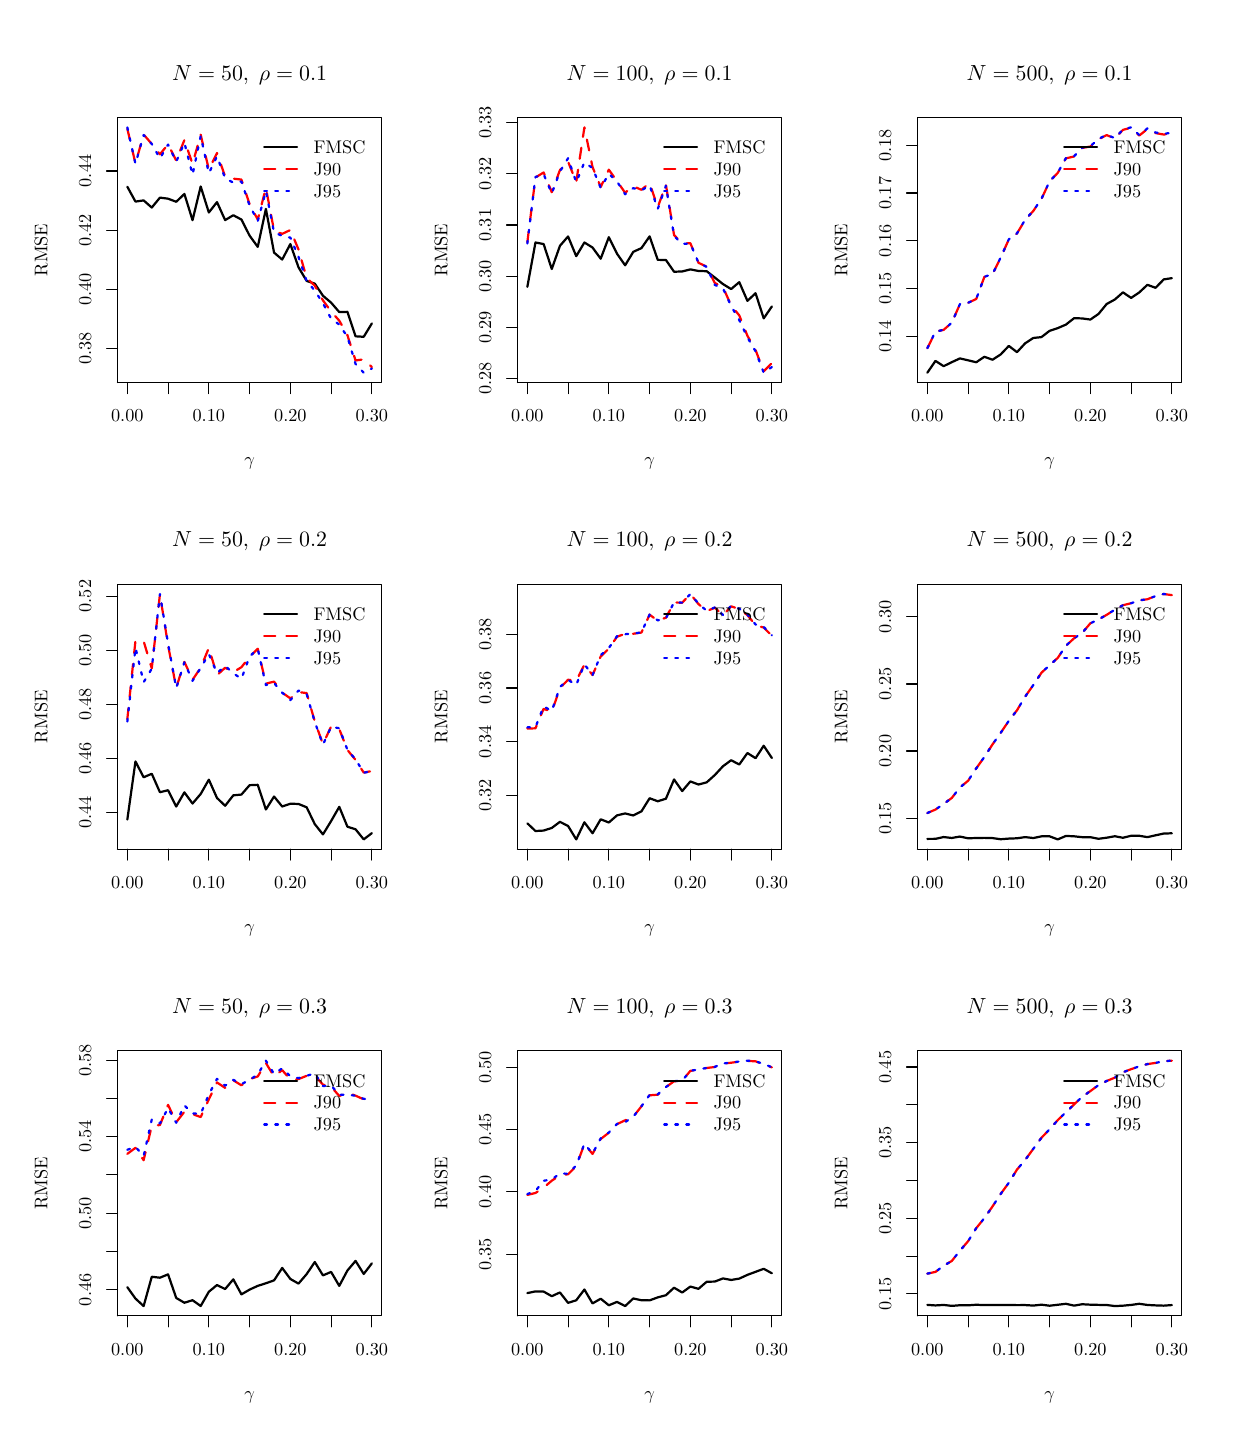
\begin{tikzpicture}[x=1pt,y=1pt]
\definecolor[named]{fillColor}{rgb}{1.00,1.00,1.00}
\path[use as bounding box,fill=fillColor,fill opacity=0.00] (0,0) rectangle (433.62,505.89);
\begin{scope}
\path[clip] ( 32.47,377.65) rectangle (127.91,473.42);
\definecolor[named]{drawColor}{rgb}{0.00,0.00,0.00}

\path[draw=drawColor,line width= 0.8pt,line join=round,line cap=round] ( 36.01,448.40) --
	( 38.95,443.04) --
	( 41.90,443.47) --
	( 44.84,440.88) --
	( 47.79,444.47) --
	( 50.73,444.09) --
	( 53.68,442.97) --
	( 56.63,445.80) --
	( 59.57,436.32) --
	( 62.52,448.50) --
	( 65.46,439.10) --
	( 68.41,442.85) --
	( 71.35,436.35) --
	( 74.30,438.11) --
	( 77.24,436.55) --
	( 80.19,430.73) --
	( 83.14,426.68) --
	( 86.08,440.41) --
	( 89.03,424.60) --
	( 91.97,422.10) --
	( 94.92,427.70) --
	( 97.86,419.31) --
	(100.81,414.37) --
	(103.75,413.40) --
	(106.70,409.01) --
	(109.65,406.52) --
	(112.59,403.11) --
	(115.54,403.20) --
	(118.48,394.36) --
	(121.43,394.18) --
	(124.37,399.02);
\end{scope}
\begin{scope}
\path[clip] (  0.00,  0.00) rectangle (433.62,505.89);
\definecolor[named]{drawColor}{rgb}{0.00,0.00,0.00}

\path[draw=drawColor,line width= 0.4pt,line join=round,line cap=round] ( 36.01,377.65) -- (124.37,377.65);

\path[draw=drawColor,line width= 0.4pt,line join=round,line cap=round] ( 36.01,377.65) -- ( 36.01,373.69);

\path[draw=drawColor,line width= 0.4pt,line join=round,line cap=round] ( 50.73,377.65) -- ( 50.73,373.69);

\path[draw=drawColor,line width= 0.4pt,line join=round,line cap=round] ( 65.46,377.65) -- ( 65.46,373.69);

\path[draw=drawColor,line width= 0.4pt,line join=round,line cap=round] ( 80.19,377.65) -- ( 80.19,373.69);

\path[draw=drawColor,line width= 0.4pt,line join=round,line cap=round] ( 94.92,377.65) -- ( 94.92,373.69);

\path[draw=drawColor,line width= 0.4pt,line join=round,line cap=round] (109.65,377.65) -- (109.65,373.69);

\path[draw=drawColor,line width= 0.4pt,line join=round,line cap=round] (124.37,377.65) -- (124.37,373.69);

\node[text=drawColor,anchor=base,inner sep=0pt, outer sep=0pt, scale=  0.66] at ( 36.01,363.40) {0.00};

\node[text=drawColor,anchor=base,inner sep=0pt, outer sep=0pt, scale=  0.66] at ( 65.46,363.40) {0.10};

\node[text=drawColor,anchor=base,inner sep=0pt, outer sep=0pt, scale=  0.66] at ( 94.92,363.40) {0.20};

\node[text=drawColor,anchor=base,inner sep=0pt, outer sep=0pt, scale=  0.66] at (124.37,363.40) {0.30};

\path[draw=drawColor,line width= 0.4pt,line join=round,line cap=round] ( 32.47,389.93) -- ( 32.47,454.11);

\path[draw=drawColor,line width= 0.4pt,line join=round,line cap=round] ( 32.47,389.93) -- ( 28.51,389.93);

\path[draw=drawColor,line width= 0.4pt,line join=round,line cap=round] ( 32.47,411.32) -- ( 28.51,411.32);

\path[draw=drawColor,line width= 0.4pt,line join=round,line cap=round] ( 32.47,432.72) -- ( 28.51,432.72);

\path[draw=drawColor,line width= 0.4pt,line join=round,line cap=round] ( 32.47,454.11) -- ( 28.51,454.11);

\node[text=drawColor,rotate= 90.00,anchor=base,inner sep=0pt, outer sep=0pt, scale=  0.66] at ( 22.97,389.93) {0.38};

\node[text=drawColor,rotate= 90.00,anchor=base,inner sep=0pt, outer sep=0pt, scale=  0.66] at ( 22.97,411.32) {0.40};

\node[text=drawColor,rotate= 90.00,anchor=base,inner sep=0pt, outer sep=0pt, scale=  0.66] at ( 22.97,432.72) {0.42};

\node[text=drawColor,rotate= 90.00,anchor=base,inner sep=0pt, outer sep=0pt, scale=  0.66] at ( 22.97,454.11) {0.44};

\path[draw=drawColor,line width= 0.4pt,line join=round,line cap=round] ( 32.47,377.65) --
	(127.91,377.65) --
	(127.91,473.42) --
	( 32.47,473.42) --
	( 32.47,377.65);
\end{scope}
\begin{scope}
\path[clip] (  0.00,337.26) rectangle (144.54,505.89);
\definecolor[named]{drawColor}{rgb}{0.00,0.00,0.00}

\node[text=drawColor,anchor=base,inner sep=0pt, outer sep=0pt, scale=  0.79] at ( 80.19,486.92) {\bfseries $N=50, \;\rho=0.1$};

\node[text=drawColor,anchor=base,inner sep=0pt, outer sep=0pt, scale=  0.66] at ( 80.19,347.56) {$\gamma$};

\node[text=drawColor,rotate= 90.00,anchor=base,inner sep=0pt, outer sep=0pt, scale=  0.66] at (  7.13,425.53) {RMSE};
\end{scope}
\begin{scope}
\path[clip] ( 32.47,377.65) rectangle (127.91,473.42);
\definecolor[named]{drawColor}{rgb}{1.00,0.00,0.00}

\path[draw=drawColor,line width= 0.8pt,dash pattern=on 4pt off 4pt ,line join=round,line cap=round] ( 36.01,469.35) --
	( 38.95,456.83) --
	( 41.90,467.26) --
	( 44.84,463.89) --
	( 47.79,460.13) --
	( 50.73,463.73) --
	( 53.68,457.89) --
	( 56.63,465.27) --
	( 59.57,456.67) --
	( 62.52,467.21) --
	( 65.46,454.64) --
	( 68.41,460.59) --
	( 71.35,452.09) --
	( 74.30,451.33) --
	( 77.24,450.99) --
	( 80.19,442.11) --
	( 83.14,436.54) --
	( 86.08,447.99) --
	( 89.03,432.52) --
	( 91.97,431.38) --
	( 94.92,432.77) --
	( 97.86,425.75) --
	(100.81,415.41) --
	(103.75,412.67) --
	(106.70,407.35) --
	(109.65,403.30) --
	(112.59,400.03) --
	(115.54,394.76) --
	(118.48,385.62) --
	(121.43,386.05) --
	(124.37,383.24);
\definecolor[named]{drawColor}{rgb}{0.00,0.00,1.00}

\path[draw=drawColor,line width= 0.8pt,dash pattern=on 1pt off 3pt ,line join=round,line cap=round] ( 36.01,469.87) --
	( 38.95,456.69) --
	( 41.90,467.11) --
	( 44.84,463.88) --
	( 47.79,458.63) --
	( 50.73,463.64) --
	( 53.68,457.45) --
	( 56.63,464.32) --
	( 59.57,452.73) --
	( 62.52,466.71) --
	( 65.46,453.28) --
	( 68.41,459.37) --
	( 71.35,451.48) --
	( 74.30,449.88) --
	( 77.24,450.29) --
	( 80.19,441.60) --
	( 83.14,435.99) --
	( 86.08,446.82) --
	( 89.03,431.92) --
	( 91.97,430.65) --
	( 94.92,430.02) --
	( 97.86,423.10) --
	(100.81,414.32) --
	(103.75,410.89) --
	(106.70,406.27) --
	(109.65,400.76) --
	(112.59,398.60) --
	(115.54,394.17) --
	(118.48,384.36) --
	(121.43,381.20) --
	(124.37,382.71);
\definecolor[named]{drawColor}{rgb}{0.00,0.00,0.00}

\path[draw=drawColor,line width= 0.8pt,line join=round,line cap=round] ( 85.47,462.63) -- ( 97.35,462.63);
\definecolor[named]{drawColor}{rgb}{1.00,0.00,0.00}

\path[draw=drawColor,line width= 0.8pt,dash pattern=on 4pt off 4pt ,line join=round,line cap=round] ( 85.47,454.71) -- ( 97.35,454.71);
\definecolor[named]{drawColor}{rgb}{0.00,0.00,1.00}

\path[draw=drawColor,line width= 0.8pt,dash pattern=on 1pt off 3pt ,line join=round,line cap=round] ( 85.47,446.79) -- ( 97.35,446.79);
\definecolor[named]{drawColor}{rgb}{0.00,0.00,0.00}

\node[text=drawColor,anchor=base west,inner sep=0pt, outer sep=0pt, scale=  0.66] at (103.29,460.35) {FMSC};

\node[text=drawColor,anchor=base west,inner sep=0pt, outer sep=0pt, scale=  0.66] at (103.29,452.43) {J90};

\node[text=drawColor,anchor=base west,inner sep=0pt, outer sep=0pt, scale=  0.66] at (103.29,444.51) {J95};
\end{scope}
\begin{scope}
\path[clip] (177.01,377.65) rectangle (272.45,473.42);
\definecolor[named]{drawColor}{rgb}{0.00,0.00,0.00}

\path[draw=drawColor,line width= 0.8pt,line join=round,line cap=round] (180.55,412.23) --
	(183.49,428.26) --
	(186.44,427.69) --
	(189.38,418.68) --
	(192.33,427.06) --
	(195.27,430.44) --
	(198.22,423.31) --
	(201.17,428.26) --
	(204.11,426.44) --
	(207.06,422.40) --
	(210.00,430.17) --
	(212.95,424.21) --
	(215.89,420.02) --
	(218.84,424.89) --
	(221.78,426.22) --
	(224.73,430.47) --
	(227.68,421.98) --
	(230.62,421.95) --
	(233.57,417.69) --
	(236.51,417.79) --
	(239.46,418.54) --
	(242.40,417.97) --
	(245.35,417.88) --
	(248.29,415.59) --
	(251.24,413.24) --
	(254.19,411.43) --
	(257.13,413.93) --
	(260.08,407.17) --
	(263.02,409.93) --
	(265.97,400.84) --
	(268.91,405.14);
\end{scope}
\begin{scope}
\path[clip] (  0.00,  0.00) rectangle (433.62,505.89);
\definecolor[named]{drawColor}{rgb}{0.00,0.00,0.00}

\path[draw=drawColor,line width= 0.4pt,line join=round,line cap=round] (180.55,377.65) -- (268.91,377.65);

\path[draw=drawColor,line width= 0.4pt,line join=round,line cap=round] (180.55,377.65) -- (180.55,373.69);

\path[draw=drawColor,line width= 0.4pt,line join=round,line cap=round] (195.27,377.65) -- (195.27,373.69);

\path[draw=drawColor,line width= 0.4pt,line join=round,line cap=round] (210.00,377.65) -- (210.00,373.69);

\path[draw=drawColor,line width= 0.4pt,line join=round,line cap=round] (224.73,377.65) -- (224.73,373.69);

\path[draw=drawColor,line width= 0.4pt,line join=round,line cap=round] (239.46,377.65) -- (239.46,373.69);

\path[draw=drawColor,line width= 0.4pt,line join=round,line cap=round] (254.19,377.65) -- (254.19,373.69);

\path[draw=drawColor,line width= 0.4pt,line join=round,line cap=round] (268.91,377.65) -- (268.91,373.69);

\node[text=drawColor,anchor=base,inner sep=0pt, outer sep=0pt, scale=  0.66] at (180.55,363.40) {0.00};

\node[text=drawColor,anchor=base,inner sep=0pt, outer sep=0pt, scale=  0.66] at (210.00,363.40) {0.10};

\node[text=drawColor,anchor=base,inner sep=0pt, outer sep=0pt, scale=  0.66] at (239.46,363.40) {0.20};

\node[text=drawColor,anchor=base,inner sep=0pt, outer sep=0pt, scale=  0.66] at (268.91,363.40) {0.30};

\path[draw=drawColor,line width= 0.4pt,line join=round,line cap=round] (177.01,379.18) -- (177.01,471.53);

\path[draw=drawColor,line width= 0.4pt,line join=round,line cap=round] (177.01,379.18) -- (173.05,379.18);

\path[draw=drawColor,line width= 0.4pt,line join=round,line cap=round] (177.01,397.65) -- (173.05,397.65);

\path[draw=drawColor,line width= 0.4pt,line join=round,line cap=round] (177.01,416.12) -- (173.05,416.12);

\path[draw=drawColor,line width= 0.4pt,line join=round,line cap=round] (177.01,434.59) -- (173.05,434.59);

\path[draw=drawColor,line width= 0.4pt,line join=round,line cap=round] (177.01,453.06) -- (173.05,453.06);

\path[draw=drawColor,line width= 0.4pt,line join=round,line cap=round] (177.01,471.53) -- (173.05,471.53);

\node[text=drawColor,rotate= 90.00,anchor=base,inner sep=0pt, outer sep=0pt, scale=  0.66] at (167.51,379.18) {0.28};

\node[text=drawColor,rotate= 90.00,anchor=base,inner sep=0pt, outer sep=0pt, scale=  0.66] at (167.51,397.65) {0.29};

\node[text=drawColor,rotate= 90.00,anchor=base,inner sep=0pt, outer sep=0pt, scale=  0.66] at (167.51,416.12) {0.30};

\node[text=drawColor,rotate= 90.00,anchor=base,inner sep=0pt, outer sep=0pt, scale=  0.66] at (167.51,434.59) {0.31};

\node[text=drawColor,rotate= 90.00,anchor=base,inner sep=0pt, outer sep=0pt, scale=  0.66] at (167.51,453.06) {0.32};

\node[text=drawColor,rotate= 90.00,anchor=base,inner sep=0pt, outer sep=0pt, scale=  0.66] at (167.51,471.53) {0.33};

\path[draw=drawColor,line width= 0.4pt,line join=round,line cap=round] (177.01,377.65) --
	(272.45,377.65) --
	(272.45,473.42) --
	(177.01,473.42) --
	(177.01,377.65);
\end{scope}
\begin{scope}
\path[clip] (144.54,337.26) rectangle (289.08,505.89);
\definecolor[named]{drawColor}{rgb}{0.00,0.00,0.00}

\node[text=drawColor,anchor=base,inner sep=0pt, outer sep=0pt, scale=  0.79] at (224.73,486.92) {\bfseries $N=100, \;\rho=0.1$};

\node[text=drawColor,anchor=base,inner sep=0pt, outer sep=0pt, scale=  0.66] at (224.73,347.56) {$\gamma$};

\node[text=drawColor,rotate= 90.00,anchor=base,inner sep=0pt, outer sep=0pt, scale=  0.66] at (151.67,425.54) {RMSE};
\end{scope}
\begin{scope}
\path[clip] (177.01,377.65) rectangle (272.45,473.42);
\definecolor[named]{drawColor}{rgb}{1.00,0.00,0.00}

\path[draw=drawColor,line width= 0.8pt,dash pattern=on 4pt off 4pt ,line join=round,line cap=round] (180.55,428.35) --
	(183.49,451.74) --
	(186.44,453.56) --
	(189.38,446.43) --
	(192.33,454.42) --
	(195.27,457.48) --
	(198.22,450.08) --
	(201.17,469.87) --
	(204.11,455.52) --
	(207.06,448.32) --
	(210.00,454.57) --
	(212.95,450.43) --
	(215.89,446.24) --
	(218.84,448.57) --
	(221.78,447.30) --
	(224.73,449.76) --
	(227.68,441.01) --
	(230.62,449.17) --
	(233.57,430.96) --
	(236.51,427.87) --
	(239.46,427.99) --
	(242.40,420.92) --
	(245.35,419.53) --
	(248.29,413.62) --
	(251.24,412.15) --
	(254.19,405.51) --
	(257.13,401.92) --
	(260.08,394.55) --
	(263.02,389.40) --
	(265.97,381.71) --
	(268.91,384.71);
\definecolor[named]{drawColor}{rgb}{0.00,0.00,1.00}

\path[draw=drawColor,line width= 0.8pt,dash pattern=on 1pt off 3pt ,line join=round,line cap=round] (180.55,427.89) --
	(183.49,451.92) --
	(186.44,452.94) --
	(189.38,445.98) --
	(192.33,453.89) --
	(195.27,458.70) --
	(198.22,450.03) --
	(201.17,457.22) --
	(204.11,455.16) --
	(207.06,447.99) --
	(210.00,453.08) --
	(212.95,450.33) --
	(215.89,445.69) --
	(218.84,447.90) --
	(221.78,447.08) --
	(224.73,448.92) --
	(227.68,440.40) --
	(230.62,448.79) --
	(233.57,430.58) --
	(236.51,427.77) --
	(239.46,427.88) --
	(242.40,420.96) --
	(245.35,419.44) --
	(248.29,412.93) --
	(251.24,411.68) --
	(254.19,405.31) --
	(257.13,400.20) --
	(260.08,393.94) --
	(263.02,388.96) --
	(265.97,381.20) --
	(268.91,383.25);
\definecolor[named]{drawColor}{rgb}{0.00,0.00,0.00}

\path[draw=drawColor,line width= 0.8pt,line join=round,line cap=round] (230.01,462.63) -- (241.89,462.63);
\definecolor[named]{drawColor}{rgb}{1.00,0.00,0.00}

\path[draw=drawColor,line width= 0.8pt,dash pattern=on 4pt off 4pt ,line join=round,line cap=round] (230.01,454.71) -- (241.89,454.71);
\definecolor[named]{drawColor}{rgb}{0.00,0.00,1.00}

\path[draw=drawColor,line width= 0.8pt,dash pattern=on 1pt off 3pt ,line join=round,line cap=round] (230.01,446.79) -- (241.89,446.79);
\definecolor[named]{drawColor}{rgb}{0.00,0.00,0.00}

\node[text=drawColor,anchor=base west,inner sep=0pt, outer sep=0pt, scale=  0.66] at (247.83,460.35) {FMSC};

\node[text=drawColor,anchor=base west,inner sep=0pt, outer sep=0pt, scale=  0.66] at (247.83,452.43) {J90};

\node[text=drawColor,anchor=base west,inner sep=0pt, outer sep=0pt, scale=  0.66] at (247.83,444.51) {J95};
\end{scope}
\begin{scope}
\path[clip] (321.55,377.65) rectangle (416.99,473.42);
\definecolor[named]{drawColor}{rgb}{0.00,0.00,0.00}

\path[draw=drawColor,line width= 0.8pt,line join=round,line cap=round] (325.09,381.20) --
	(328.03,385.47) --
	(330.98,383.57) --
	(333.92,385.01) --
	(336.87,386.37) --
	(339.81,385.69) --
	(342.76,384.98) --
	(345.71,386.96) --
	(348.65,385.89) --
	(351.60,387.82) --
	(354.54,390.89) --
	(357.49,388.63) --
	(360.43,391.83) --
	(363.38,393.76) --
	(366.32,394.07) --
	(369.27,396.35) --
	(372.22,397.32) --
	(375.16,398.59) --
	(378.11,400.90) --
	(381.05,400.82) --
	(384.00,400.41) --
	(386.94,402.44) --
	(389.89,406.03) --
	(392.83,407.65) --
	(395.78,410.24) --
	(398.73,408.23) --
	(401.67,410.22) --
	(404.62,412.97) --
	(407.56,411.88) --
	(410.51,414.92) --
	(413.45,415.38);
\end{scope}
\begin{scope}
\path[clip] (  0.00,  0.00) rectangle (433.62,505.89);
\definecolor[named]{drawColor}{rgb}{0.00,0.00,0.00}

\path[draw=drawColor,line width= 0.4pt,line join=round,line cap=round] (325.09,377.65) -- (413.45,377.65);

\path[draw=drawColor,line width= 0.4pt,line join=round,line cap=round] (325.09,377.65) -- (325.09,373.69);

\path[draw=drawColor,line width= 0.4pt,line join=round,line cap=round] (339.81,377.65) -- (339.81,373.69);

\path[draw=drawColor,line width= 0.4pt,line join=round,line cap=round] (354.54,377.65) -- (354.54,373.69);

\path[draw=drawColor,line width= 0.4pt,line join=round,line cap=round] (369.27,377.65) -- (369.27,373.69);

\path[draw=drawColor,line width= 0.4pt,line join=round,line cap=round] (384.00,377.65) -- (384.00,373.69);

\path[draw=drawColor,line width= 0.4pt,line join=round,line cap=round] (398.73,377.65) -- (398.73,373.69);

\path[draw=drawColor,line width= 0.4pt,line join=round,line cap=round] (413.45,377.65) -- (413.45,373.69);

\node[text=drawColor,anchor=base,inner sep=0pt, outer sep=0pt, scale=  0.66] at (325.09,363.40) {0.00};

\node[text=drawColor,anchor=base,inner sep=0pt, outer sep=0pt, scale=  0.66] at (354.54,363.40) {0.10};

\node[text=drawColor,anchor=base,inner sep=0pt, outer sep=0pt, scale=  0.66] at (384.00,363.40) {0.20};

\node[text=drawColor,anchor=base,inner sep=0pt, outer sep=0pt, scale=  0.66] at (413.45,363.40) {0.30};

\path[draw=drawColor,line width= 0.4pt,line join=round,line cap=round] (321.55,394.27) -- (321.55,463.45);

\path[draw=drawColor,line width= 0.4pt,line join=round,line cap=round] (321.55,394.27) -- (317.59,394.27);

\path[draw=drawColor,line width= 0.4pt,line join=round,line cap=round] (321.55,411.56) -- (317.59,411.56);

\path[draw=drawColor,line width= 0.4pt,line join=round,line cap=round] (321.55,428.86) -- (317.59,428.86);

\path[draw=drawColor,line width= 0.4pt,line join=round,line cap=round] (321.55,446.15) -- (317.59,446.15);

\path[draw=drawColor,line width= 0.4pt,line join=round,line cap=round] (321.55,463.45) -- (317.59,463.45);

\node[text=drawColor,rotate= 90.00,anchor=base,inner sep=0pt, outer sep=0pt, scale=  0.66] at (312.05,394.27) {0.14};

\node[text=drawColor,rotate= 90.00,anchor=base,inner sep=0pt, outer sep=0pt, scale=  0.66] at (312.05,411.56) {0.15};

\node[text=drawColor,rotate= 90.00,anchor=base,inner sep=0pt, outer sep=0pt, scale=  0.66] at (312.05,428.86) {0.16};

\node[text=drawColor,rotate= 90.00,anchor=base,inner sep=0pt, outer sep=0pt, scale=  0.66] at (312.05,446.15) {0.17};

\node[text=drawColor,rotate= 90.00,anchor=base,inner sep=0pt, outer sep=0pt, scale=  0.66] at (312.05,463.45) {0.18};

\path[draw=drawColor,line width= 0.4pt,line join=round,line cap=round] (321.55,377.65) --
	(416.99,377.65) --
	(416.99,473.42) --
	(321.55,473.42) --
	(321.55,377.65);
\end{scope}
\begin{scope}
\path[clip] (289.08,337.26) rectangle (433.62,505.89);
\definecolor[named]{drawColor}{rgb}{0.00,0.00,0.00}

\node[text=drawColor,anchor=base,inner sep=0pt, outer sep=0pt, scale=  0.79] at (369.27,486.92) {\bfseries $N=500, \;\rho=0.1$};

\node[text=drawColor,anchor=base,inner sep=0pt, outer sep=0pt, scale=  0.66] at (369.27,347.56) {$\gamma$};

\node[text=drawColor,rotate= 90.00,anchor=base,inner sep=0pt, outer sep=0pt, scale=  0.66] at (296.21,425.53) {RMSE};
\end{scope}
\begin{scope}
\path[clip] (321.55,377.65) rectangle (416.99,473.42);
\definecolor[named]{drawColor}{rgb}{1.00,0.00,0.00}

\path[draw=drawColor,line width= 0.8pt,dash pattern=on 4pt off 4pt ,line join=round,line cap=round] (325.09,390.05) --
	(328.03,396.03) --
	(330.98,396.69) --
	(333.92,399.26) --
	(336.87,405.99) --
	(339.81,406.46) --
	(342.76,407.84) --
	(345.71,415.86) --
	(348.65,416.85) --
	(351.60,422.79) --
	(354.54,429.40) --
	(357.49,431.54) --
	(360.43,436.43) --
	(363.38,439.66) --
	(366.32,444.00) --
	(369.27,450.32) --
	(372.22,453.42) --
	(375.16,458.66) --
	(378.11,459.33) --
	(381.05,462.43) --
	(384.00,462.93) --
	(386.94,465.52) --
	(389.89,467.08) --
	(392.83,465.81) --
	(395.78,468.96) --
	(398.73,469.73) --
	(401.67,466.91) --
	(404.62,469.27) --
	(407.56,467.79) --
	(410.51,467.27) --
	(413.45,467.70);
\definecolor[named]{drawColor}{rgb}{0.00,0.00,1.00}

\path[draw=drawColor,line width= 0.8pt,dash pattern=on 1pt off 3pt ,line join=round,line cap=round] (325.09,390.09) --
	(328.03,396.04) --
	(330.98,396.71) --
	(333.92,399.27) --
	(336.87,406.00) --
	(339.81,406.47) --
	(342.76,407.85) --
	(345.71,415.86) --
	(348.65,416.88) --
	(351.60,422.82) --
	(354.54,429.42) --
	(357.49,431.57) --
	(360.43,436.47) --
	(363.38,439.70) --
	(366.32,444.02) --
	(369.27,450.38) --
	(372.22,453.48) --
	(375.16,458.73) --
	(378.11,459.43) --
	(381.05,462.53) --
	(384.00,463.06) --
	(386.94,465.67) --
	(389.89,467.21) --
	(392.83,465.94) --
	(395.78,469.10) --
	(398.73,469.87) --
	(401.67,467.06) --
	(404.62,469.50) --
	(407.56,468.01) --
	(410.51,467.52) --
	(413.45,467.92);
\definecolor[named]{drawColor}{rgb}{0.00,0.00,0.00}

\path[draw=drawColor,line width= 0.8pt,line join=round,line cap=round] (374.55,462.63) -- (386.43,462.63);
\definecolor[named]{drawColor}{rgb}{1.00,0.00,0.00}

\path[draw=drawColor,line width= 0.8pt,dash pattern=on 4pt off 4pt ,line join=round,line cap=round] (374.55,454.71) -- (386.43,454.71);
\definecolor[named]{drawColor}{rgb}{0.00,0.00,1.00}

\path[draw=drawColor,line width= 0.8pt,dash pattern=on 1pt off 3pt ,line join=round,line cap=round] (374.55,446.79) -- (386.43,446.79);
\definecolor[named]{drawColor}{rgb}{0.00,0.00,0.00}

\node[text=drawColor,anchor=base west,inner sep=0pt, outer sep=0pt, scale=  0.66] at (392.37,460.35) {FMSC};

\node[text=drawColor,anchor=base west,inner sep=0pt, outer sep=0pt, scale=  0.66] at (392.37,452.43) {J90};

\node[text=drawColor,anchor=base west,inner sep=0pt, outer sep=0pt, scale=  0.66] at (392.37,444.51) {J95};
\end{scope}
\begin{scope}
\path[clip] ( 32.47,209.02) rectangle (127.91,304.79);
\definecolor[named]{drawColor}{rgb}{0.00,0.00,0.00}

\path[draw=drawColor,line width= 0.8pt,line join=round,line cap=round] ( 36.01,219.74) --
	( 38.95,240.74) --
	( 41.90,235.02) --
	( 44.84,236.28) --
	( 47.79,229.62) --
	( 50.73,230.33) --
	( 53.68,224.45) --
	( 56.63,229.57) --
	( 59.57,225.53) --
	( 62.52,228.99) --
	( 65.46,234.16) --
	( 68.41,227.54) --
	( 71.35,224.72) --
	( 74.30,228.49) --
	( 77.24,228.77) --
	( 80.19,232.16) --
	( 83.14,232.29) --
	( 86.08,223.38) --
	( 89.03,228.06) --
	( 91.97,224.45) --
	( 94.92,225.46) --
	( 97.86,225.38) --
	(100.81,224.17) --
	(103.75,218.08) --
	(106.70,214.38) --
	(109.65,219.20) --
	(112.59,224.33) --
	(115.54,217.16) --
	(118.48,216.22) --
	(121.43,212.57) --
	(124.37,214.84);
\end{scope}
\begin{scope}
\path[clip] (  0.00,  0.00) rectangle (433.62,505.89);
\definecolor[named]{drawColor}{rgb}{0.00,0.00,0.00}

\path[draw=drawColor,line width= 0.4pt,line join=round,line cap=round] ( 36.01,209.02) -- (124.37,209.02);

\path[draw=drawColor,line width= 0.4pt,line join=round,line cap=round] ( 36.01,209.02) -- ( 36.01,205.06);

\path[draw=drawColor,line width= 0.4pt,line join=round,line cap=round] ( 50.73,209.02) -- ( 50.73,205.06);

\path[draw=drawColor,line width= 0.4pt,line join=round,line cap=round] ( 65.46,209.02) -- ( 65.46,205.06);

\path[draw=drawColor,line width= 0.4pt,line join=round,line cap=round] ( 80.19,209.02) -- ( 80.19,205.06);

\path[draw=drawColor,line width= 0.4pt,line join=round,line cap=round] ( 94.92,209.02) -- ( 94.92,205.06);

\path[draw=drawColor,line width= 0.4pt,line join=round,line cap=round] (109.65,209.02) -- (109.65,205.06);

\path[draw=drawColor,line width= 0.4pt,line join=round,line cap=round] (124.37,209.02) -- (124.37,205.06);

\node[text=drawColor,anchor=base,inner sep=0pt, outer sep=0pt, scale=  0.66] at ( 36.01,194.77) {0.00};

\node[text=drawColor,anchor=base,inner sep=0pt, outer sep=0pt, scale=  0.66] at ( 65.46,194.77) {0.10};

\node[text=drawColor,anchor=base,inner sep=0pt, outer sep=0pt, scale=  0.66] at ( 94.92,194.77) {0.20};

\node[text=drawColor,anchor=base,inner sep=0pt, outer sep=0pt, scale=  0.66] at (124.37,194.77) {0.30};

\path[draw=drawColor,line width= 0.4pt,line join=round,line cap=round] ( 32.47,222.38) -- ( 32.47,300.49);

\path[draw=drawColor,line width= 0.4pt,line join=round,line cap=round] ( 32.47,222.38) -- ( 28.51,222.38);

\path[draw=drawColor,line width= 0.4pt,line join=round,line cap=round] ( 32.47,241.91) -- ( 28.51,241.91);

\path[draw=drawColor,line width= 0.4pt,line join=round,line cap=round] ( 32.47,261.44) -- ( 28.51,261.44);

\path[draw=drawColor,line width= 0.4pt,line join=round,line cap=round] ( 32.47,280.96) -- ( 28.51,280.96);

\path[draw=drawColor,line width= 0.4pt,line join=round,line cap=round] ( 32.47,300.49) -- ( 28.51,300.49);

\node[text=drawColor,rotate= 90.00,anchor=base,inner sep=0pt, outer sep=0pt, scale=  0.66] at ( 22.97,222.38) {0.44};

\node[text=drawColor,rotate= 90.00,anchor=base,inner sep=0pt, outer sep=0pt, scale=  0.66] at ( 22.97,241.91) {0.46};

\node[text=drawColor,rotate= 90.00,anchor=base,inner sep=0pt, outer sep=0pt, scale=  0.66] at ( 22.97,261.44) {0.48};

\node[text=drawColor,rotate= 90.00,anchor=base,inner sep=0pt, outer sep=0pt, scale=  0.66] at ( 22.97,280.96) {0.50};

\node[text=drawColor,rotate= 90.00,anchor=base,inner sep=0pt, outer sep=0pt, scale=  0.66] at ( 22.97,300.49) {0.52};

\path[draw=drawColor,line width= 0.4pt,line join=round,line cap=round] ( 32.47,209.02) --
	(127.91,209.02) --
	(127.91,304.79) --
	( 32.47,304.79) --
	( 32.47,209.02);
\end{scope}
\begin{scope}
\path[clip] (  0.00,168.63) rectangle (144.54,337.26);
\definecolor[named]{drawColor}{rgb}{0.00,0.00,0.00}

\node[text=drawColor,anchor=base,inner sep=0pt, outer sep=0pt, scale=  0.79] at ( 80.19,318.29) {\bfseries $N=50, \;\rho=0.2$};

\node[text=drawColor,anchor=base,inner sep=0pt, outer sep=0pt, scale=  0.66] at ( 80.19,178.93) {$\gamma$};

\node[text=drawColor,rotate= 90.00,anchor=base,inner sep=0pt, outer sep=0pt, scale=  0.66] at (  7.13,256.90) {RMSE};
\end{scope}
\begin{scope}
\path[clip] ( 32.47,209.02) rectangle (127.91,304.79);
\definecolor[named]{drawColor}{rgb}{1.00,0.00,0.00}

\path[draw=drawColor,line width= 0.8pt,dash pattern=on 4pt off 4pt ,line join=round,line cap=round] ( 36.01,256.06) --
	( 38.95,284.37) --
	( 41.90,284.21) --
	( 44.84,274.37) --
	( 47.79,301.13) --
	( 50.73,282.74) --
	( 53.68,267.35) --
	( 56.63,276.72) --
	( 59.57,270.25) --
	( 62.52,274.58) --
	( 65.46,281.77) --
	( 68.41,271.92) --
	( 71.35,274.60) --
	( 74.30,273.01) --
	( 77.24,274.80) --
	( 80.19,278.52) --
	( 83.14,281.45) --
	( 86.08,268.87) --
	( 89.03,269.57) --
	( 91.97,265.61) --
	( 94.92,263.53) --
	( 97.86,265.79) --
	(100.81,265.45) --
	(103.75,255.20) --
	(106.70,246.99) --
	(109.65,253.38) --
	(112.59,252.44) --
	(115.54,244.88) --
	(118.48,241.30) --
	(121.43,236.71) --
	(124.37,237.28);
\definecolor[named]{drawColor}{rgb}{0.00,0.00,1.00}

\path[draw=drawColor,line width= 0.8pt,dash pattern=on 1pt off 3pt ,line join=round,line cap=round] ( 36.01,255.15) --
	( 38.95,281.88) --
	( 41.90,269.36) --
	( 44.84,274.25) --
	( 47.79,301.24) --
	( 50.73,283.33) --
	( 53.68,267.24) --
	( 56.63,276.56) --
	( 59.57,269.86) --
	( 62.52,274.53) --
	( 65.46,279.56) --
	( 68.41,272.64) --
	( 71.35,275.25) --
	( 74.30,272.60) --
	( 77.24,270.61) --
	( 80.19,278.67) --
	( 83.14,281.40) --
	( 86.08,268.34) --
	( 89.03,269.07) --
	( 91.97,265.59) --
	( 94.92,262.90) --
	( 97.86,266.36) --
	(100.81,265.11) --
	(103.75,254.98) --
	(106.70,246.81) --
	(109.65,253.26) --
	(112.59,252.74) --
	(115.54,244.95) --
	(118.48,241.50) --
	(121.43,236.65) --
	(124.37,237.22);
\definecolor[named]{drawColor}{rgb}{0.00,0.00,0.00}

\path[draw=drawColor,line width= 0.8pt,line join=round,line cap=round] ( 85.47,294.00) -- ( 97.35,294.00);
\definecolor[named]{drawColor}{rgb}{1.00,0.00,0.00}

\path[draw=drawColor,line width= 0.8pt,dash pattern=on 4pt off 4pt ,line join=round,line cap=round] ( 85.47,286.08) -- ( 97.35,286.08);
\definecolor[named]{drawColor}{rgb}{0.00,0.00,1.00}

\path[draw=drawColor,line width= 0.8pt,dash pattern=on 1pt off 3pt ,line join=round,line cap=round] ( 85.47,278.16) -- ( 97.35,278.16);
\definecolor[named]{drawColor}{rgb}{0.00,0.00,0.00}

\node[text=drawColor,anchor=base west,inner sep=0pt, outer sep=0pt, scale=  0.66] at (103.29,291.72) {FMSC};

\node[text=drawColor,anchor=base west,inner sep=0pt, outer sep=0pt, scale=  0.66] at (103.29,283.80) {J90};

\node[text=drawColor,anchor=base west,inner sep=0pt, outer sep=0pt, scale=  0.66] at (103.29,275.88) {J95};
\end{scope}
\begin{scope}
\path[clip] (177.01,209.02) rectangle (272.45,304.79);
\definecolor[named]{drawColor}{rgb}{0.00,0.00,0.00}

\path[draw=drawColor,line width= 0.8pt,line join=round,line cap=round] (180.55,218.38) --
	(183.49,215.60) --
	(186.44,215.76) --
	(189.38,216.71) --
	(192.33,218.92) --
	(195.27,217.42) --
	(198.22,212.57) --
	(201.17,218.75) --
	(204.11,214.78) --
	(207.06,219.84) --
	(210.00,218.67) --
	(212.95,221.25) --
	(215.89,221.95) --
	(218.84,221.22) --
	(221.78,222.70) --
	(224.73,227.44) --
	(227.68,226.35) --
	(230.62,227.27) --
	(233.57,234.23) --
	(236.51,230.03) --
	(239.46,233.52) --
	(242.40,232.40) --
	(245.35,233.18) --
	(248.29,235.82) --
	(251.24,239.00) --
	(254.19,241.18) --
	(257.13,239.63) --
	(260.08,243.78) --
	(263.02,241.92) --
	(265.97,246.42) --
	(268.91,241.99);
\end{scope}
\begin{scope}
\path[clip] (  0.00,  0.00) rectangle (433.62,505.89);
\definecolor[named]{drawColor}{rgb}{0.00,0.00,0.00}

\path[draw=drawColor,line width= 0.4pt,line join=round,line cap=round] (180.55,209.02) -- (268.91,209.02);

\path[draw=drawColor,line width= 0.4pt,line join=round,line cap=round] (180.55,209.02) -- (180.55,205.06);

\path[draw=drawColor,line width= 0.4pt,line join=round,line cap=round] (195.27,209.02) -- (195.27,205.06);

\path[draw=drawColor,line width= 0.4pt,line join=round,line cap=round] (210.00,209.02) -- (210.00,205.06);

\path[draw=drawColor,line width= 0.4pt,line join=round,line cap=round] (224.73,209.02) -- (224.73,205.06);

\path[draw=drawColor,line width= 0.4pt,line join=round,line cap=round] (239.46,209.02) -- (239.46,205.06);

\path[draw=drawColor,line width= 0.4pt,line join=round,line cap=round] (254.19,209.02) -- (254.19,205.06);

\path[draw=drawColor,line width= 0.4pt,line join=round,line cap=round] (268.91,209.02) -- (268.91,205.06);

\node[text=drawColor,anchor=base,inner sep=0pt, outer sep=0pt, scale=  0.66] at (180.55,194.77) {0.00};

\node[text=drawColor,anchor=base,inner sep=0pt, outer sep=0pt, scale=  0.66] at (210.00,194.77) {0.10};

\node[text=drawColor,anchor=base,inner sep=0pt, outer sep=0pt, scale=  0.66] at (239.46,194.77) {0.20};

\node[text=drawColor,anchor=base,inner sep=0pt, outer sep=0pt, scale=  0.66] at (268.91,194.77) {0.30};

\path[draw=drawColor,line width= 0.4pt,line join=round,line cap=round] (177.01,228.35) -- (177.01,286.73);

\path[draw=drawColor,line width= 0.4pt,line join=round,line cap=round] (177.01,228.35) -- (173.05,228.35);

\path[draw=drawColor,line width= 0.4pt,line join=round,line cap=round] (177.01,247.81) -- (173.05,247.81);

\path[draw=drawColor,line width= 0.4pt,line join=round,line cap=round] (177.01,267.27) -- (173.05,267.27);

\path[draw=drawColor,line width= 0.4pt,line join=round,line cap=round] (177.01,286.73) -- (173.05,286.73);

\node[text=drawColor,rotate= 90.00,anchor=base,inner sep=0pt, outer sep=0pt, scale=  0.66] at (167.51,228.35) {0.32};

\node[text=drawColor,rotate= 90.00,anchor=base,inner sep=0pt, outer sep=0pt, scale=  0.66] at (167.51,247.81) {0.34};

\node[text=drawColor,rotate= 90.00,anchor=base,inner sep=0pt, outer sep=0pt, scale=  0.66] at (167.51,267.27) {0.36};

\node[text=drawColor,rotate= 90.00,anchor=base,inner sep=0pt, outer sep=0pt, scale=  0.66] at (167.51,286.73) {0.38};

\path[draw=drawColor,line width= 0.4pt,line join=round,line cap=round] (177.01,209.02) --
	(272.45,209.02) --
	(272.45,304.79) --
	(177.01,304.79) --
	(177.01,209.02);
\end{scope}
\begin{scope}
\path[clip] (144.54,168.63) rectangle (289.08,337.26);
\definecolor[named]{drawColor}{rgb}{0.00,0.00,0.00}

\node[text=drawColor,anchor=base,inner sep=0pt, outer sep=0pt, scale=  0.79] at (224.73,318.29) {\bfseries $N=100, \;\rho=0.2$};

\node[text=drawColor,anchor=base,inner sep=0pt, outer sep=0pt, scale=  0.66] at (224.73,178.93) {$\gamma$};

\node[text=drawColor,rotate= 90.00,anchor=base,inner sep=0pt, outer sep=0pt, scale=  0.66] at (151.67,256.90) {RMSE};
\end{scope}
\begin{scope}
\path[clip] (177.01,209.02) rectangle (272.45,304.79);
\definecolor[named]{drawColor}{rgb}{1.00,0.00,0.00}

\path[draw=drawColor,line width= 0.8pt,dash pattern=on 4pt off 4pt ,line join=round,line cap=round] (180.55,252.62) --
	(183.49,252.71) --
	(186.44,259.76) --
	(189.38,258.64) --
	(192.33,267.25) --
	(195.27,270.27) --
	(198.22,269.84) --
	(201.17,275.71) --
	(204.11,271.96) --
	(207.06,278.67) --
	(210.00,281.49) --
	(212.95,285.81) --
	(215.89,286.87) --
	(218.84,286.88) --
	(221.78,287.32) --
	(224.73,293.75) --
	(227.68,291.61) --
	(230.62,292.68) --
	(233.57,298.16) --
	(236.51,298.10) --
	(239.46,301.24) --
	(242.40,297.61) --
	(245.35,295.06) --
	(248.29,296.27) --
	(251.24,293.55) --
	(254.19,296.79) --
	(257.13,295.79) --
	(260.08,293.62) --
	(263.02,289.95) --
	(265.97,289.12) --
	(268.91,286.16);
\definecolor[named]{drawColor}{rgb}{0.00,0.00,1.00}

\path[draw=drawColor,line width= 0.8pt,dash pattern=on 1pt off 3pt ,line join=round,line cap=round] (180.55,253.07) --
	(183.49,253.12) --
	(186.44,260.66) --
	(189.38,258.95) --
	(192.33,267.67) --
	(195.27,270.20) --
	(198.22,268.37) --
	(201.17,275.86) --
	(204.11,271.93) --
	(207.06,279.14) --
	(210.00,281.72) --
	(212.95,286.00) --
	(215.89,286.72) --
	(218.84,286.96) --
	(221.78,287.37) --
	(224.73,293.83) --
	(227.68,291.72) --
	(230.62,292.42) --
	(233.57,298.23) --
	(236.51,298.12) --
	(239.46,301.23) --
	(242.40,297.77) --
	(245.35,295.17) --
	(248.29,296.39) --
	(251.24,293.69) --
	(254.19,297.00) --
	(257.13,295.92) --
	(260.08,293.84) --
	(263.02,290.23) --
	(265.97,289.31) --
	(268.91,286.34);
\definecolor[named]{drawColor}{rgb}{0.00,0.00,0.00}

\path[draw=drawColor,line width= 0.8pt,line join=round,line cap=round] (230.01,294.00) -- (241.89,294.00);
\definecolor[named]{drawColor}{rgb}{1.00,0.00,0.00}

\path[draw=drawColor,line width= 0.8pt,dash pattern=on 4pt off 4pt ,line join=round,line cap=round] (230.01,286.08) -- (241.89,286.08);
\definecolor[named]{drawColor}{rgb}{0.00,0.00,1.00}

\path[draw=drawColor,line width= 0.8pt,dash pattern=on 1pt off 3pt ,line join=round,line cap=round] (230.01,278.16) -- (241.89,278.16);
\definecolor[named]{drawColor}{rgb}{0.00,0.00,0.00}

\node[text=drawColor,anchor=base west,inner sep=0pt, outer sep=0pt, scale=  0.66] at (247.83,291.72) {FMSC};

\node[text=drawColor,anchor=base west,inner sep=0pt, outer sep=0pt, scale=  0.66] at (247.83,283.80) {J90};

\node[text=drawColor,anchor=base west,inner sep=0pt, outer sep=0pt, scale=  0.66] at (247.83,275.88) {J95};
\end{scope}
\begin{scope}
\path[clip] (321.55,209.02) rectangle (416.99,304.79);
\definecolor[named]{drawColor}{rgb}{0.00,0.00,0.00}

\path[draw=drawColor,line width= 0.8pt,line join=round,line cap=round] (325.09,212.75) --
	(328.03,212.77) --
	(330.98,213.42) --
	(333.92,213.09) --
	(336.87,213.59) --
	(339.81,212.97) --
	(342.76,213.07) --
	(345.71,213.12) --
	(348.65,213.04) --
	(351.60,212.63) --
	(354.54,212.86) --
	(357.49,212.97) --
	(360.43,213.40) --
	(363.38,213.06) --
	(366.32,213.67) --
	(369.27,213.68) --
	(372.22,212.57) --
	(375.16,213.82) --
	(378.11,213.69) --
	(381.05,213.37) --
	(384.00,213.38) --
	(386.94,212.79) --
	(389.89,213.18) --
	(392.83,213.71) --
	(395.78,213.16) --
	(398.73,213.89) --
	(401.67,213.88) --
	(404.62,213.39) --
	(407.56,214.05) --
	(410.51,214.68) --
	(413.45,214.78);
\end{scope}
\begin{scope}
\path[clip] (  0.00,  0.00) rectangle (433.62,505.89);
\definecolor[named]{drawColor}{rgb}{0.00,0.00,0.00}

\path[draw=drawColor,line width= 0.4pt,line join=round,line cap=round] (325.09,209.02) -- (413.45,209.02);

\path[draw=drawColor,line width= 0.4pt,line join=round,line cap=round] (325.09,209.02) -- (325.09,205.06);

\path[draw=drawColor,line width= 0.4pt,line join=round,line cap=round] (339.81,209.02) -- (339.81,205.06);

\path[draw=drawColor,line width= 0.4pt,line join=round,line cap=round] (354.54,209.02) -- (354.54,205.06);

\path[draw=drawColor,line width= 0.4pt,line join=round,line cap=round] (369.27,209.02) -- (369.27,205.06);

\path[draw=drawColor,line width= 0.4pt,line join=round,line cap=round] (384.00,209.02) -- (384.00,205.06);

\path[draw=drawColor,line width= 0.4pt,line join=round,line cap=round] (398.73,209.02) -- (398.73,205.06);

\path[draw=drawColor,line width= 0.4pt,line join=round,line cap=round] (413.45,209.02) -- (413.45,205.06);

\node[text=drawColor,anchor=base,inner sep=0pt, outer sep=0pt, scale=  0.66] at (325.09,194.77) {0.00};

\node[text=drawColor,anchor=base,inner sep=0pt, outer sep=0pt, scale=  0.66] at (354.54,194.77) {0.10};

\node[text=drawColor,anchor=base,inner sep=0pt, outer sep=0pt, scale=  0.66] at (384.00,194.77) {0.20};

\node[text=drawColor,anchor=base,inner sep=0pt, outer sep=0pt, scale=  0.66] at (413.45,194.77) {0.30};

\path[draw=drawColor,line width= 0.4pt,line join=round,line cap=round] (321.55,220.25) -- (321.55,292.99);

\path[draw=drawColor,line width= 0.4pt,line join=round,line cap=round] (321.55,220.25) -- (317.59,220.25);

\path[draw=drawColor,line width= 0.4pt,line join=round,line cap=round] (321.55,244.50) -- (317.59,244.50);

\path[draw=drawColor,line width= 0.4pt,line join=round,line cap=round] (321.55,268.74) -- (317.59,268.74);

\path[draw=drawColor,line width= 0.4pt,line join=round,line cap=round] (321.55,292.99) -- (317.59,292.99);

\node[text=drawColor,rotate= 90.00,anchor=base,inner sep=0pt, outer sep=0pt, scale=  0.66] at (312.05,220.25) {0.15};

\node[text=drawColor,rotate= 90.00,anchor=base,inner sep=0pt, outer sep=0pt, scale=  0.66] at (312.05,244.50) {0.20};

\node[text=drawColor,rotate= 90.00,anchor=base,inner sep=0pt, outer sep=0pt, scale=  0.66] at (312.05,268.74) {0.25};

\node[text=drawColor,rotate= 90.00,anchor=base,inner sep=0pt, outer sep=0pt, scale=  0.66] at (312.05,292.99) {0.30};

\path[draw=drawColor,line width= 0.4pt,line join=round,line cap=round] (321.55,209.02) --
	(416.99,209.02) --
	(416.99,304.79) --
	(321.55,304.79) --
	(321.55,209.02);
\end{scope}
\begin{scope}
\path[clip] (289.08,168.63) rectangle (433.62,337.26);
\definecolor[named]{drawColor}{rgb}{0.00,0.00,0.00}

\node[text=drawColor,anchor=base,inner sep=0pt, outer sep=0pt, scale=  0.79] at (369.27,318.29) {\bfseries $N=500, \;\rho=0.2$};

\node[text=drawColor,anchor=base,inner sep=0pt, outer sep=0pt, scale=  0.66] at (369.27,178.93) {$\gamma$};

\node[text=drawColor,rotate= 90.00,anchor=base,inner sep=0pt, outer sep=0pt, scale=  0.66] at (296.21,256.90) {RMSE};
\end{scope}
\begin{scope}
\path[clip] (321.55,209.02) rectangle (416.99,304.79);
\definecolor[named]{drawColor}{rgb}{1.00,0.00,0.00}

\path[draw=drawColor,line width= 0.8pt,dash pattern=on 4pt off 4pt ,line join=round,line cap=round] (325.09,222.10) --
	(328.03,223.36) --
	(330.98,225.38) --
	(333.92,227.54) --
	(336.87,231.34) --
	(339.81,233.75) --
	(342.76,238.24) --
	(345.71,242.37) --
	(348.65,246.91) --
	(351.60,251.09) --
	(354.54,255.42) --
	(357.49,259.23) --
	(360.43,264.16) --
	(363.38,268.34) --
	(366.32,272.80) --
	(369.27,275.51) --
	(372.22,278.16) --
	(375.16,282.53) --
	(378.11,285.24) --
	(381.05,287.19) --
	(384.00,290.66) --
	(386.94,292.06) --
	(389.89,293.71) --
	(392.83,295.59) --
	(395.78,297.19) --
	(398.73,297.91) --
	(401.67,298.95) --
	(404.62,299.35) --
	(407.56,300.50) --
	(410.51,301.24) --
	(413.45,300.84);
\definecolor[named]{drawColor}{rgb}{0.00,0.00,1.00}

\path[draw=drawColor,line width= 0.8pt,dash pattern=on 1pt off 3pt ,line join=round,line cap=round] (325.09,222.10) --
	(328.03,223.36) --
	(330.98,225.38) --
	(333.92,227.54) --
	(336.87,231.34) --
	(339.81,233.75) --
	(342.76,238.24) --
	(345.71,242.37) --
	(348.65,246.91) --
	(351.60,251.09) --
	(354.54,255.42) --
	(357.49,259.23) --
	(360.43,264.16) --
	(363.38,268.34) --
	(366.32,272.80) --
	(369.27,275.51) --
	(372.22,278.16) --
	(375.16,282.53) --
	(378.11,285.24) --
	(381.05,287.19) --
	(384.00,290.66) --
	(386.94,292.06) --
	(389.89,293.71) --
	(392.83,295.59) --
	(395.78,297.19) --
	(398.73,297.91) --
	(401.67,298.95) --
	(404.62,299.35) --
	(407.56,300.50) --
	(410.51,301.24) --
	(413.45,300.84);
\definecolor[named]{drawColor}{rgb}{0.00,0.00,0.00}

\path[draw=drawColor,line width= 0.8pt,line join=round,line cap=round] (374.55,294.00) -- (386.43,294.00);
\definecolor[named]{drawColor}{rgb}{1.00,0.00,0.00}

\path[draw=drawColor,line width= 0.8pt,dash pattern=on 4pt off 4pt ,line join=round,line cap=round] (374.55,286.08) -- (386.43,286.08);
\definecolor[named]{drawColor}{rgb}{0.00,0.00,1.00}

\path[draw=drawColor,line width= 0.8pt,dash pattern=on 1pt off 3pt ,line join=round,line cap=round] (374.55,278.16) -- (386.43,278.16);
\definecolor[named]{drawColor}{rgb}{0.00,0.00,0.00}

\node[text=drawColor,anchor=base west,inner sep=0pt, outer sep=0pt, scale=  0.66] at (392.37,291.72) {FMSC};

\node[text=drawColor,anchor=base west,inner sep=0pt, outer sep=0pt, scale=  0.66] at (392.37,283.80) {J90};

\node[text=drawColor,anchor=base west,inner sep=0pt, outer sep=0pt, scale=  0.66] at (392.37,275.88) {J95};
\end{scope}
\begin{scope}
\path[clip] ( 32.47, 40.39) rectangle (127.91,136.16);
\definecolor[named]{drawColor}{rgb}{0.00,0.00,0.00}

\path[draw=drawColor,line width= 0.8pt,line join=round,line cap=round] ( 36.01, 50.77) --
	( 38.95, 46.65) --
	( 41.90, 43.94) --
	( 44.84, 54.53) --
	( 47.79, 54.19) --
	( 50.73, 55.40) --
	( 53.68, 46.87) --
	( 56.63, 45.14) --
	( 59.57, 46.06) --
	( 62.52, 43.96) --
	( 65.46, 49.11) --
	( 68.41, 51.54) --
	( 71.35, 50.09) --
	( 74.30, 53.60) --
	( 77.24, 48.17) --
	( 80.19, 49.89) --
	( 83.14, 51.24) --
	( 86.08, 52.18) --
	( 89.03, 53.23) --
	( 91.97, 57.72) --
	( 94.92, 53.73) --
	( 97.86, 52.06) --
	(100.81, 55.49) --
	(103.75, 59.86) --
	(106.70, 55.03) --
	(109.65, 56.28) --
	(112.59, 51.24) --
	(115.54, 56.79) --
	(118.48, 60.26) --
	(121.43, 55.54) --
	(124.37, 59.37);
\end{scope}
\begin{scope}
\path[clip] (  0.00,  0.00) rectangle (433.62,505.89);
\definecolor[named]{drawColor}{rgb}{0.00,0.00,0.00}

\path[draw=drawColor,line width= 0.4pt,line join=round,line cap=round] ( 36.01, 40.39) -- (124.37, 40.39);

\path[draw=drawColor,line width= 0.4pt,line join=round,line cap=round] ( 36.01, 40.39) -- ( 36.01, 36.43);

\path[draw=drawColor,line width= 0.4pt,line join=round,line cap=round] ( 50.73, 40.39) -- ( 50.73, 36.43);

\path[draw=drawColor,line width= 0.4pt,line join=round,line cap=round] ( 65.46, 40.39) -- ( 65.46, 36.43);

\path[draw=drawColor,line width= 0.4pt,line join=round,line cap=round] ( 80.19, 40.39) -- ( 80.19, 36.43);

\path[draw=drawColor,line width= 0.4pt,line join=round,line cap=round] ( 94.92, 40.39) -- ( 94.92, 36.43);

\path[draw=drawColor,line width= 0.4pt,line join=round,line cap=round] (109.65, 40.39) -- (109.65, 36.43);

\path[draw=drawColor,line width= 0.4pt,line join=round,line cap=round] (124.37, 40.39) -- (124.37, 36.43);

\node[text=drawColor,anchor=base,inner sep=0pt, outer sep=0pt, scale=  0.66] at ( 36.01, 26.14) {0.00};

\node[text=drawColor,anchor=base,inner sep=0pt, outer sep=0pt, scale=  0.66] at ( 65.46, 26.14) {0.10};

\node[text=drawColor,anchor=base,inner sep=0pt, outer sep=0pt, scale=  0.66] at ( 94.92, 26.14) {0.20};

\node[text=drawColor,anchor=base,inner sep=0pt, outer sep=0pt, scale=  0.66] at (124.37, 26.14) {0.30};

\path[draw=drawColor,line width= 0.4pt,line join=round,line cap=round] ( 32.47, 49.83) -- ( 32.47,132.82);

\path[draw=drawColor,line width= 0.4pt,line join=round,line cap=round] ( 32.47, 49.83) -- ( 28.51, 49.83);

\path[draw=drawColor,line width= 0.4pt,line join=round,line cap=round] ( 32.47, 63.66) -- ( 28.51, 63.66);

\path[draw=drawColor,line width= 0.4pt,line join=round,line cap=round] ( 32.47, 77.50) -- ( 28.51, 77.50);

\path[draw=drawColor,line width= 0.4pt,line join=round,line cap=round] ( 32.47, 91.33) -- ( 28.51, 91.33);

\path[draw=drawColor,line width= 0.4pt,line join=round,line cap=round] ( 32.47,105.16) -- ( 28.51,105.16);

\path[draw=drawColor,line width= 0.4pt,line join=round,line cap=round] ( 32.47,118.99) -- ( 28.51,118.99);

\path[draw=drawColor,line width= 0.4pt,line join=round,line cap=round] ( 32.47,132.82) -- ( 28.51,132.82);

\node[text=drawColor,rotate= 90.00,anchor=base,inner sep=0pt, outer sep=0pt, scale=  0.66] at ( 22.97, 49.83) {0.46};

\node[text=drawColor,rotate= 90.00,anchor=base,inner sep=0pt, outer sep=0pt, scale=  0.66] at ( 22.97, 77.50) {0.50};

\node[text=drawColor,rotate= 90.00,anchor=base,inner sep=0pt, outer sep=0pt, scale=  0.66] at ( 22.97,105.16) {0.54};

\node[text=drawColor,rotate= 90.00,anchor=base,inner sep=0pt, outer sep=0pt, scale=  0.66] at ( 22.97,132.82) {0.58};

\path[draw=drawColor,line width= 0.4pt,line join=round,line cap=round] ( 32.47, 40.39) --
	(127.91, 40.39) --
	(127.91,136.16) --
	( 32.47,136.16) --
	( 32.47, 40.39);
\end{scope}
\begin{scope}
\path[clip] (  0.00,  0.00) rectangle (144.54,168.63);
\definecolor[named]{drawColor}{rgb}{0.00,0.00,0.00}

\node[text=drawColor,anchor=base,inner sep=0pt, outer sep=0pt, scale=  0.79] at ( 80.19,149.66) {\bfseries $N=50, \;\rho=0.3$};

\node[text=drawColor,anchor=base,inner sep=0pt, outer sep=0pt, scale=  0.66] at ( 80.19, 10.30) {$\gamma$};

\node[text=drawColor,rotate= 90.00,anchor=base,inner sep=0pt, outer sep=0pt, scale=  0.66] at (  7.13, 88.27) {RMSE};
\end{scope}
\begin{scope}
\path[clip] ( 32.47, 40.39) rectangle (127.91,136.16);
\definecolor[named]{drawColor}{rgb}{1.00,0.00,0.00}

\path[draw=drawColor,line width= 0.8pt,dash pattern=on 4pt off 4pt ,line join=round,line cap=round] ( 36.01, 98.94) --
	( 38.95,101.11) --
	( 41.90, 96.65) --
	( 44.84,109.08) --
	( 47.79,109.35) --
	( 50.73,116.65) --
	( 53.68,110.36) --
	( 56.63,114.17) --
	( 59.57,113.29) --
	( 62.52,112.25) --
	( 65.46,118.63) --
	( 68.41,124.75) --
	( 71.35,122.78) --
	( 74.30,125.52) --
	( 77.24,123.71) --
	( 80.19,125.95) --
	( 83.14,126.91) --
	( 86.08,131.78) --
	( 89.03,126.91) --
	( 91.97,129.22) --
	( 94.92,125.74) --
	( 97.86,125.96) --
	(100.81,127.14) --
	(103.75,127.19) --
	(106.70,123.95) --
	(109.65,123.24) --
	(112.59,119.86) --
	(115.54,121.05) --
	(118.48,119.97) --
	(121.43,118.65) --
	(124.37,118.00);
\definecolor[named]{drawColor}{rgb}{0.00,0.00,1.00}

\path[draw=drawColor,line width= 0.8pt,dash pattern=on 1pt off 3pt ,line join=round,line cap=round] ( 36.01,100.41) --
	( 38.95,101.46) --
	( 41.90, 98.19) --
	( 44.84,111.34) --
	( 47.79,109.91) --
	( 50.73,115.49) --
	( 53.68,110.17) --
	( 56.63,116.45) --
	( 59.57,113.56) --
	( 62.52,113.39) --
	( 65.46,120.39) --
	( 68.41,126.05) --
	( 71.35,123.58) --
	( 74.30,125.69) --
	( 77.24,124.11) --
	( 80.19,125.70) --
	( 83.14,127.61) --
	( 86.08,132.61) --
	( 89.03,127.80) --
	( 91.97,129.86) --
	( 94.92,126.98) --
	( 97.86,126.30) --
	(100.81,127.15) --
	(103.75,128.04) --
	(106.70,123.46) --
	(109.65,123.62) --
	(112.59,120.32) --
	(115.54,120.30) --
	(118.48,119.95) --
	(121.43,118.84) --
	(124.37,118.49);
\definecolor[named]{drawColor}{rgb}{0.00,0.00,0.00}

\path[draw=drawColor,line width= 0.8pt,line join=round,line cap=round] ( 85.47,125.37) -- ( 97.35,125.37);
\definecolor[named]{drawColor}{rgb}{1.00,0.00,0.00}

\path[draw=drawColor,line width= 0.8pt,dash pattern=on 4pt off 4pt ,line join=round,line cap=round] ( 85.47,117.45) -- ( 97.35,117.45);
\definecolor[named]{drawColor}{rgb}{0.00,0.00,1.00}

\path[draw=drawColor,line width= 0.8pt,dash pattern=on 1pt off 3pt ,line join=round,line cap=round] ( 85.47,109.53) -- ( 97.35,109.53);
\definecolor[named]{drawColor}{rgb}{0.00,0.00,0.00}

\node[text=drawColor,anchor=base west,inner sep=0pt, outer sep=0pt, scale=  0.66] at (103.29,123.09) {FMSC};

\node[text=drawColor,anchor=base west,inner sep=0pt, outer sep=0pt, scale=  0.66] at (103.29,115.17) {J90};

\node[text=drawColor,anchor=base west,inner sep=0pt, outer sep=0pt, scale=  0.66] at (103.29,107.25) {J95};
\end{scope}
\begin{scope}
\path[clip] (177.01, 40.39) rectangle (272.45,136.16);
\definecolor[named]{drawColor}{rgb}{0.00,0.00,0.00}

\path[draw=drawColor,line width= 0.8pt,line join=round,line cap=round] (180.55, 48.63) --
	(183.49, 49.24) --
	(186.44, 49.17) --
	(189.38, 47.51) --
	(192.33, 48.86) --
	(195.27, 45.10) --
	(198.22, 46.03) --
	(201.17, 49.92) --
	(204.11, 44.90) --
	(207.06, 46.60) --
	(210.00, 44.23) --
	(212.95, 45.44) --
	(215.89, 43.94) --
	(218.84, 46.69) --
	(221.78, 46.04) --
	(224.73, 46.00) --
	(227.68, 47.08) --
	(230.62, 47.86) --
	(233.57, 50.58) --
	(236.51, 48.83) --
	(239.46, 50.99) --
	(242.40, 50.17) --
	(245.35, 52.73) --
	(248.29, 52.79) --
	(251.24, 53.93) --
	(254.19, 53.38) --
	(257.13, 53.86) --
	(260.08, 55.22) --
	(263.02, 56.31) --
	(265.97, 57.41) --
	(268.91, 55.79);
\end{scope}
\begin{scope}
\path[clip] (  0.00,  0.00) rectangle (433.62,505.89);
\definecolor[named]{drawColor}{rgb}{0.00,0.00,0.00}

\path[draw=drawColor,line width= 0.4pt,line join=round,line cap=round] (180.55, 40.39) -- (268.91, 40.39);

\path[draw=drawColor,line width= 0.4pt,line join=round,line cap=round] (180.55, 40.39) -- (180.55, 36.43);

\path[draw=drawColor,line width= 0.4pt,line join=round,line cap=round] (195.27, 40.39) -- (195.27, 36.43);

\path[draw=drawColor,line width= 0.4pt,line join=round,line cap=round] (210.00, 40.39) -- (210.00, 36.43);

\path[draw=drawColor,line width= 0.4pt,line join=round,line cap=round] (224.73, 40.39) -- (224.73, 36.43);

\path[draw=drawColor,line width= 0.4pt,line join=round,line cap=round] (239.46, 40.39) -- (239.46, 36.43);

\path[draw=drawColor,line width= 0.4pt,line join=round,line cap=round] (254.19, 40.39) -- (254.19, 36.43);

\path[draw=drawColor,line width= 0.4pt,line join=round,line cap=round] (268.91, 40.39) -- (268.91, 36.43);

\node[text=drawColor,anchor=base,inner sep=0pt, outer sep=0pt, scale=  0.66] at (180.55, 26.14) {0.00};

\node[text=drawColor,anchor=base,inner sep=0pt, outer sep=0pt, scale=  0.66] at (210.00, 26.14) {0.10};

\node[text=drawColor,anchor=base,inner sep=0pt, outer sep=0pt, scale=  0.66] at (239.46, 26.14) {0.20};

\node[text=drawColor,anchor=base,inner sep=0pt, outer sep=0pt, scale=  0.66] at (268.91, 26.14) {0.30};

\path[draw=drawColor,line width= 0.4pt,line join=round,line cap=round] (177.01, 62.65) -- (177.01,130.24);

\path[draw=drawColor,line width= 0.4pt,line join=round,line cap=round] (177.01, 62.65) -- (173.05, 62.65);

\path[draw=drawColor,line width= 0.4pt,line join=round,line cap=round] (177.01, 85.18) -- (173.05, 85.18);

\path[draw=drawColor,line width= 0.4pt,line join=round,line cap=round] (177.01,107.71) -- (173.05,107.71);

\path[draw=drawColor,line width= 0.4pt,line join=round,line cap=round] (177.01,130.24) -- (173.05,130.24);

\node[text=drawColor,rotate= 90.00,anchor=base,inner sep=0pt, outer sep=0pt, scale=  0.66] at (167.51, 62.65) {0.35};

\node[text=drawColor,rotate= 90.00,anchor=base,inner sep=0pt, outer sep=0pt, scale=  0.66] at (167.51, 85.18) {0.40};

\node[text=drawColor,rotate= 90.00,anchor=base,inner sep=0pt, outer sep=0pt, scale=  0.66] at (167.51,107.71) {0.45};

\node[text=drawColor,rotate= 90.00,anchor=base,inner sep=0pt, outer sep=0pt, scale=  0.66] at (167.51,130.24) {0.50};

\path[draw=drawColor,line width= 0.4pt,line join=round,line cap=round] (177.01, 40.39) --
	(272.45, 40.39) --
	(272.45,136.16) --
	(177.01,136.16) --
	(177.01, 40.39);
\end{scope}
\begin{scope}
\path[clip] (144.54,  0.00) rectangle (289.08,168.63);
\definecolor[named]{drawColor}{rgb}{0.00,0.00,0.00}

\node[text=drawColor,anchor=base,inner sep=0pt, outer sep=0pt, scale=  0.79] at (224.73,149.66) {\bfseries $N=100, \;\rho=0.3$};

\node[text=drawColor,anchor=base,inner sep=0pt, outer sep=0pt, scale=  0.66] at (224.73, 10.30) {$\gamma$};

\node[text=drawColor,rotate= 90.00,anchor=base,inner sep=0pt, outer sep=0pt, scale=  0.66] at (151.67, 88.27) {RMSE};
\end{scope}
\begin{scope}
\path[clip] (177.01, 40.39) rectangle (272.45,136.16);
\definecolor[named]{drawColor}{rgb}{1.00,0.00,0.00}

\path[draw=drawColor,line width= 0.8pt,dash pattern=on 4pt off 4pt ,line join=round,line cap=round] (180.55, 84.10) --
	(183.49, 84.81) --
	(186.44, 86.74) --
	(189.38, 89.25) --
	(192.33, 91.22) --
	(195.27, 91.57) --
	(198.22, 94.49) --
	(201.17,102.48) --
	(204.11, 98.92) --
	(207.06,104.29) --
	(210.00,106.59) --
	(212.95,109.68) --
	(215.89,111.06) --
	(218.84,112.39) --
	(221.78,116.11) --
	(224.73,120.10) --
	(227.68,120.32) --
	(230.62,123.05) --
	(233.57,125.16) --
	(236.51,125.39) --
	(239.46,128.93) --
	(242.40,129.41) --
	(245.35,129.97) --
	(248.29,130.33) --
	(251.24,131.55) --
	(254.19,131.87) --
	(257.13,132.27) --
	(260.08,132.54) --
	(263.02,132.37) --
	(265.97,131.35) --
	(268.91,130.18);
\definecolor[named]{drawColor}{rgb}{0.00,0.00,1.00}

\path[draw=drawColor,line width= 0.8pt,dash pattern=on 1pt off 3pt ,line join=round,line cap=round] (180.55, 84.40) --
	(183.49, 85.52) --
	(186.44, 89.22) --
	(189.38, 89.70) --
	(192.33, 91.84) --
	(195.27, 91.78) --
	(198.22, 94.76) --
	(201.17,102.58) --
	(204.11, 99.04) --
	(207.06,104.53) --
	(210.00,106.65) --
	(212.95,109.77) --
	(215.89,110.41) --
	(218.84,112.39) --
	(221.78,116.12) --
	(224.73,120.24) --
	(227.68,120.43) --
	(230.62,123.08) --
	(233.57,125.19) --
	(236.51,125.41) --
	(239.46,128.96) --
	(242.40,129.43) --
	(245.35,129.99) --
	(248.29,130.37) --
	(251.24,131.61) --
	(254.19,131.90) --
	(257.13,132.32) --
	(260.08,132.61) --
	(263.02,132.40) --
	(265.97,131.40) --
	(268.91,130.24);
\definecolor[named]{drawColor}{rgb}{0.00,0.00,0.00}

\path[draw=drawColor,line width= 0.8pt,line join=round,line cap=round] (230.01,125.37) -- (241.89,125.37);
\definecolor[named]{drawColor}{rgb}{1.00,0.00,0.00}

\path[draw=drawColor,line width= 0.8pt,dash pattern=on 4pt off 4pt ,line join=round,line cap=round] (230.01,117.45) -- (241.89,117.45);
\definecolor[named]{drawColor}{rgb}{0.00,0.00,1.00}

\path[draw=drawColor,line width= 0.8pt,dash pattern=on 1pt off 3pt ,line join=round,line cap=round] (230.01,109.53) -- (241.89,109.53);
\definecolor[named]{drawColor}{rgb}{0.00,0.00,0.00}

\node[text=drawColor,anchor=base west,inner sep=0pt, outer sep=0pt, scale=  0.66] at (247.83,123.09) {FMSC};

\node[text=drawColor,anchor=base west,inner sep=0pt, outer sep=0pt, scale=  0.66] at (247.83,115.17) {J90};

\node[text=drawColor,anchor=base west,inner sep=0pt, outer sep=0pt, scale=  0.66] at (247.83,107.25) {J95};
\end{scope}
\begin{scope}
\path[clip] (321.55, 40.39) rectangle (416.99,136.16);
\definecolor[named]{drawColor}{rgb}{0.00,0.00,0.00}

\path[draw=drawColor,line width= 0.8pt,line join=round,line cap=round] (325.09, 44.37) --
	(328.03, 44.17) --
	(330.98, 44.35) --
	(333.92, 44.01) --
	(336.87, 44.24) --
	(339.81, 44.21) --
	(342.76, 44.42) --
	(345.71, 44.29) --
	(348.65, 44.35) --
	(351.60, 44.36) --
	(354.54, 44.34) --
	(357.49, 44.28) --
	(360.43, 44.30) --
	(363.38, 44.12) --
	(366.32, 44.44) --
	(369.27, 44.07) --
	(372.22, 44.41) --
	(375.16, 44.76) --
	(378.11, 44.10) --
	(381.05, 44.60) --
	(384.00, 44.44) --
	(386.94, 44.37) --
	(389.89, 44.33) --
	(392.83, 43.94) --
	(395.78, 44.08) --
	(398.73, 44.35) --
	(401.67, 44.77) --
	(404.62, 44.34) --
	(407.56, 44.19) --
	(410.51, 44.09) --
	(413.45, 44.30);
\end{scope}
\begin{scope}
\path[clip] (  0.00,  0.00) rectangle (433.62,505.89);
\definecolor[named]{drawColor}{rgb}{0.00,0.00,0.00}

\path[draw=drawColor,line width= 0.4pt,line join=round,line cap=round] (325.09, 40.39) -- (413.45, 40.39);

\path[draw=drawColor,line width= 0.4pt,line join=round,line cap=round] (325.09, 40.39) -- (325.09, 36.43);

\path[draw=drawColor,line width= 0.4pt,line join=round,line cap=round] (339.81, 40.39) -- (339.81, 36.43);

\path[draw=drawColor,line width= 0.4pt,line join=round,line cap=round] (354.54, 40.39) -- (354.54, 36.43);

\path[draw=drawColor,line width= 0.4pt,line join=round,line cap=round] (369.27, 40.39) -- (369.27, 36.43);

\path[draw=drawColor,line width= 0.4pt,line join=round,line cap=round] (384.00, 40.39) -- (384.00, 36.43);

\path[draw=drawColor,line width= 0.4pt,line join=round,line cap=round] (398.73, 40.39) -- (398.73, 36.43);

\path[draw=drawColor,line width= 0.4pt,line join=round,line cap=round] (413.45, 40.39) -- (413.45, 36.43);

\node[text=drawColor,anchor=base,inner sep=0pt, outer sep=0pt, scale=  0.66] at (325.09, 26.14) {0.00};

\node[text=drawColor,anchor=base,inner sep=0pt, outer sep=0pt, scale=  0.66] at (354.54, 26.14) {0.10};

\node[text=drawColor,anchor=base,inner sep=0pt, outer sep=0pt, scale=  0.66] at (384.00, 26.14) {0.20};

\node[text=drawColor,anchor=base,inner sep=0pt, outer sep=0pt, scale=  0.66] at (413.45, 26.14) {0.30};

\path[draw=drawColor,line width= 0.4pt,line join=round,line cap=round] (321.55, 48.33) -- (321.55,130.32);

\path[draw=drawColor,line width= 0.4pt,line join=round,line cap=round] (321.55, 48.33) -- (317.59, 48.33);

\path[draw=drawColor,line width= 0.4pt,line join=round,line cap=round] (321.55, 61.99) -- (317.59, 61.99);

\path[draw=drawColor,line width= 0.4pt,line join=round,line cap=round] (321.55, 75.66) -- (317.59, 75.66);

\path[draw=drawColor,line width= 0.4pt,line join=round,line cap=round] (321.55, 89.32) -- (317.59, 89.32);

\path[draw=drawColor,line width= 0.4pt,line join=round,line cap=round] (321.55,102.99) -- (317.59,102.99);

\path[draw=drawColor,line width= 0.4pt,line join=round,line cap=round] (321.55,116.65) -- (317.59,116.65);

\path[draw=drawColor,line width= 0.4pt,line join=round,line cap=round] (321.55,130.32) -- (317.59,130.32);

\node[text=drawColor,rotate= 90.00,anchor=base,inner sep=0pt, outer sep=0pt, scale=  0.66] at (312.05, 48.33) {0.15};

\node[text=drawColor,rotate= 90.00,anchor=base,inner sep=0pt, outer sep=0pt, scale=  0.66] at (312.05, 75.66) {0.25};

\node[text=drawColor,rotate= 90.00,anchor=base,inner sep=0pt, outer sep=0pt, scale=  0.66] at (312.05,102.99) {0.35};

\node[text=drawColor,rotate= 90.00,anchor=base,inner sep=0pt, outer sep=0pt, scale=  0.66] at (312.05,130.32) {0.45};

\path[draw=drawColor,line width= 0.4pt,line join=round,line cap=round] (321.55, 40.39) --
	(416.99, 40.39) --
	(416.99,136.16) --
	(321.55,136.16) --
	(321.55, 40.39);
\end{scope}
\begin{scope}
\path[clip] (289.08,  0.00) rectangle (433.62,168.63);
\definecolor[named]{drawColor}{rgb}{0.00,0.00,0.00}

\node[text=drawColor,anchor=base,inner sep=0pt, outer sep=0pt, scale=  0.79] at (369.27,149.66) {\bfseries $N=500, \;\rho=0.3$};

\node[text=drawColor,anchor=base,inner sep=0pt, outer sep=0pt, scale=  0.66] at (369.27, 10.30) {$\gamma$};

\node[text=drawColor,rotate= 90.00,anchor=base,inner sep=0pt, outer sep=0pt, scale=  0.66] at (296.21, 88.27) {RMSE};
\end{scope}
\begin{scope}
\path[clip] (321.55, 40.39) rectangle (416.99,136.16);
\definecolor[named]{drawColor}{rgb}{1.00,0.00,0.00}

\path[draw=drawColor,line width= 0.8pt,dash pattern=on 4pt off 4pt ,line join=round,line cap=round] (325.09, 55.66) --
	(328.03, 56.29) --
	(330.98, 58.51) --
	(333.92, 60.24) --
	(336.87, 63.95) --
	(339.81, 67.37) --
	(342.76, 72.09) --
	(345.71, 75.73) --
	(348.65, 79.95) --
	(351.60, 84.47) --
	(354.54, 88.50) --
	(357.49, 93.27) --
	(360.43, 96.73) --
	(363.38,100.76) --
	(366.32,104.75) --
	(369.27,107.82) --
	(372.22,111.14) --
	(375.16,113.97) --
	(378.11,116.79) --
	(381.05,119.57) --
	(384.00,121.62) --
	(386.94,123.79) --
	(389.89,125.26) --
	(392.83,126.48) --
	(395.78,128.42) --
	(398.73,129.54) --
	(401.67,130.57) --
	(404.62,131.38) --
	(407.56,131.80) --
	(410.51,132.43) --
	(413.45,132.61);
\definecolor[named]{drawColor}{rgb}{0.00,0.00,1.00}

\path[draw=drawColor,line width= 0.8pt,dash pattern=on 1pt off 3pt ,line join=round,line cap=round] (325.09, 55.66) --
	(328.03, 56.29) --
	(330.98, 58.51) --
	(333.92, 60.24) --
	(336.87, 63.95) --
	(339.81, 67.37) --
	(342.76, 72.09) --
	(345.71, 75.73) --
	(348.65, 79.95) --
	(351.60, 84.47) --
	(354.54, 88.50) --
	(357.49, 93.27) --
	(360.43, 96.73) --
	(363.38,100.76) --
	(366.32,104.75) --
	(369.27,107.82) --
	(372.22,111.14) --
	(375.16,113.97) --
	(378.11,116.79) --
	(381.05,119.57) --
	(384.00,121.62) --
	(386.94,123.79) --
	(389.89,125.26) --
	(392.83,126.48) --
	(395.78,128.42) --
	(398.73,129.54) --
	(401.67,130.57) --
	(404.62,131.38) --
	(407.56,131.80) --
	(410.51,132.43) --
	(413.45,132.61);
\definecolor[named]{drawColor}{rgb}{0.00,0.00,0.00}

\path[draw=drawColor,line width= 0.8pt,line join=round,line cap=round] (374.55,125.37) -- (386.43,125.37);
\definecolor[named]{drawColor}{rgb}{1.00,0.00,0.00}

\path[draw=drawColor,line width= 0.8pt,dash pattern=on 4pt off 4pt ,line join=round,line cap=round] (374.55,117.45) -- (386.43,117.45);
\definecolor[named]{drawColor}{rgb}{0.00,0.00,1.00}

\path[draw=drawColor,line width= 0.8pt,dash pattern=on 1pt off 3pt ,line join=round,line cap=round] (374.55,109.53) -- (386.43,109.53);
\definecolor[named]{drawColor}{rgb}{0.00,0.00,0.00}

\node[text=drawColor,anchor=base west,inner sep=0pt, outer sep=0pt, scale=  0.66] at (392.37,123.09) {FMSC};

\node[text=drawColor,anchor=base west,inner sep=0pt, outer sep=0pt, scale=  0.66] at (392.37,115.17) {J90};

\node[text=drawColor,anchor=base west,inner sep=0pt, outer sep=0pt, scale=  0.66] at (392.37,107.25) {J95};
\end{scope}
\end{tikzpicture}

	\caption{Choose IVs simulation.}
\end{figure}

\begin{figure}
\centering
	% Created by tikzDevice version 0.7.0 on 2014-07-01 17:48:20
% !TEX encoding = UTF-8 Unicode
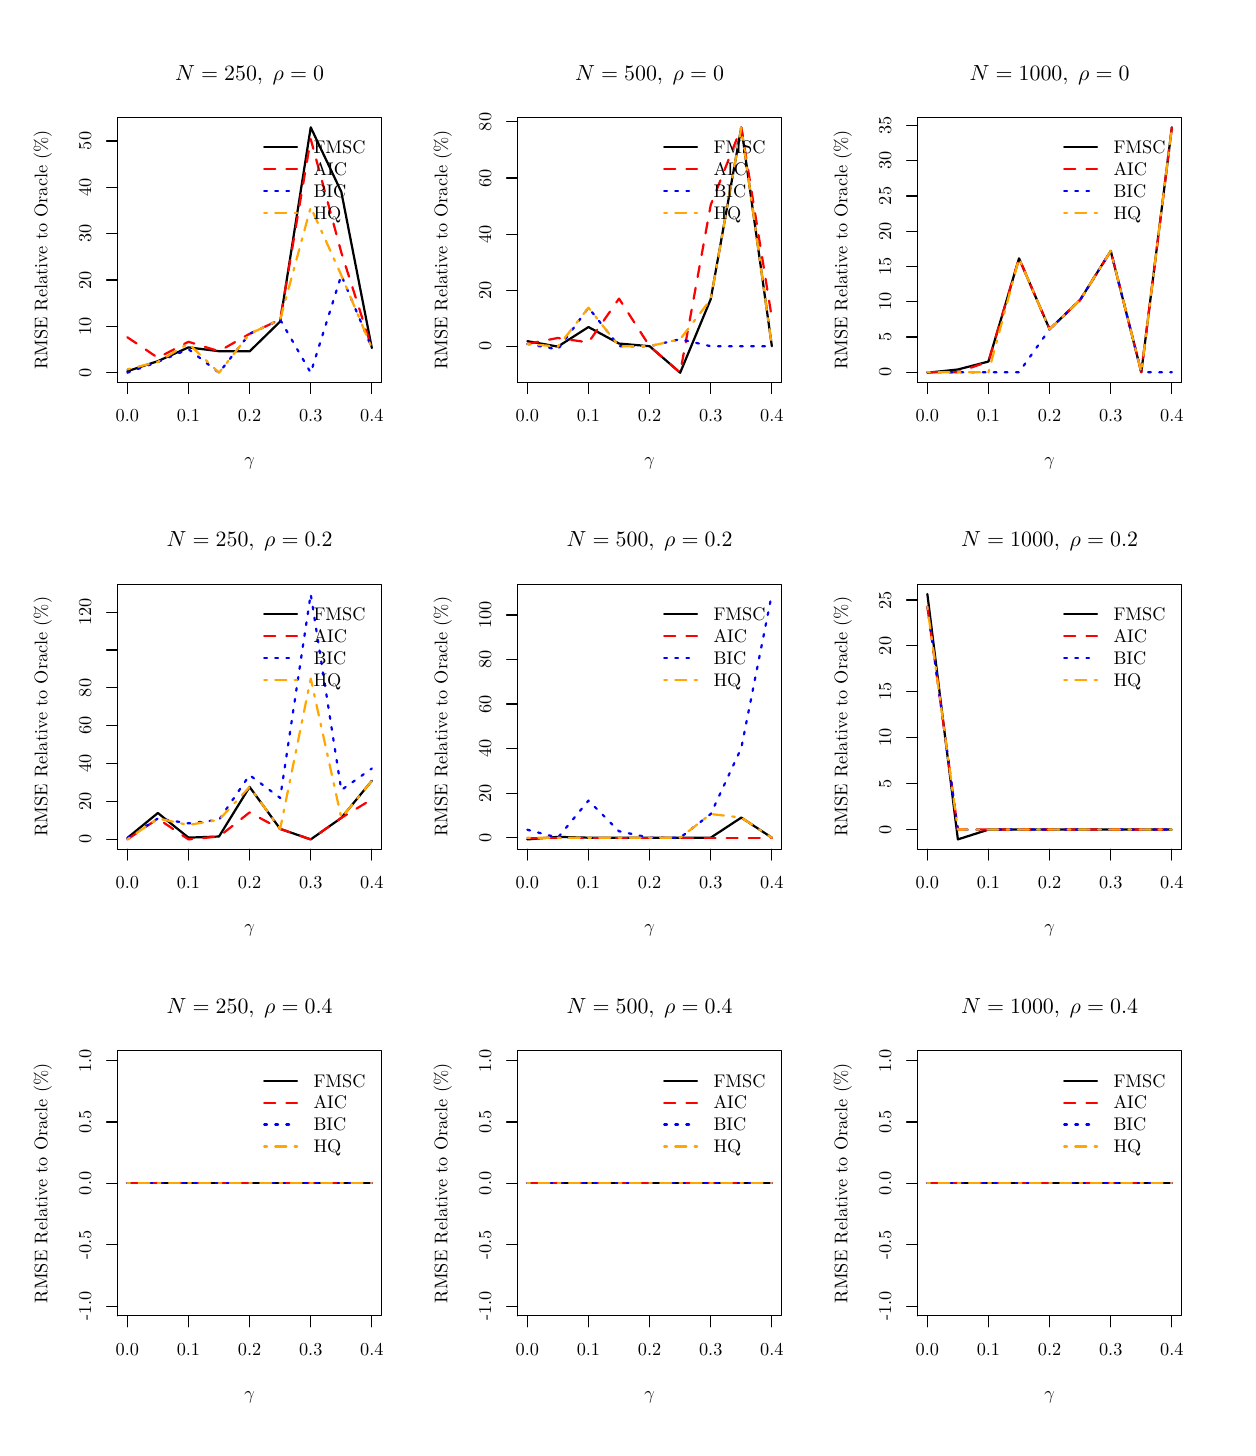
\begin{tikzpicture}[x=1pt,y=1pt]
\definecolor[named]{fillColor}{rgb}{1.00,1.00,1.00}
\path[use as bounding box,fill=fillColor,fill opacity=0.00] (0,0) rectangle (433.62,505.89);
\begin{scope}
\path[clip] ( 32.47,377.65) rectangle (127.91,473.42);
\definecolor[named]{drawColor}{rgb}{0.00,0.00,0.00}

\path[draw=drawColor,line width= 0.8pt,line join=round,line cap=round] ( 36.01,381.73) --
	( 47.05,385.39) --
	( 58.10,390.36) --
	( 69.14,388.97) --
	( 80.19,388.92) --
	( 91.24,399.70) --
	(102.28,469.87) --
	(113.33,446.56) --
	(124.37,390.09);
\end{scope}
\begin{scope}
\path[clip] (  0.00,  0.00) rectangle (433.62,505.89);
\definecolor[named]{drawColor}{rgb}{0.00,0.00,0.00}

\path[draw=drawColor,line width= 0.4pt,line join=round,line cap=round] ( 36.01,377.65) -- (124.37,377.65);

\path[draw=drawColor,line width= 0.4pt,line join=round,line cap=round] ( 36.01,377.65) -- ( 36.01,373.69);

\path[draw=drawColor,line width= 0.4pt,line join=round,line cap=round] ( 58.10,377.65) -- ( 58.10,373.69);

\path[draw=drawColor,line width= 0.4pt,line join=round,line cap=round] ( 80.19,377.65) -- ( 80.19,373.69);

\path[draw=drawColor,line width= 0.4pt,line join=round,line cap=round] (102.28,377.65) -- (102.28,373.69);

\path[draw=drawColor,line width= 0.4pt,line join=round,line cap=round] (124.37,377.65) -- (124.37,373.69);

\node[text=drawColor,anchor=base,inner sep=0pt, outer sep=0pt, scale=  0.66] at ( 36.01,363.40) {0.0};

\node[text=drawColor,anchor=base,inner sep=0pt, outer sep=0pt, scale=  0.66] at ( 58.10,363.40) {0.1};

\node[text=drawColor,anchor=base,inner sep=0pt, outer sep=0pt, scale=  0.66] at ( 80.19,363.40) {0.2};

\node[text=drawColor,anchor=base,inner sep=0pt, outer sep=0pt, scale=  0.66] at (102.28,363.40) {0.3};

\node[text=drawColor,anchor=base,inner sep=0pt, outer sep=0pt, scale=  0.66] at (124.37,363.40) {0.4};

\path[draw=drawColor,line width= 0.4pt,line join=round,line cap=round] ( 32.47,381.20) -- ( 32.47,464.94);

\path[draw=drawColor,line width= 0.4pt,line join=round,line cap=round] ( 32.47,381.20) -- ( 28.51,381.20);

\path[draw=drawColor,line width= 0.4pt,line join=round,line cap=round] ( 32.47,397.95) -- ( 28.51,397.95);

\path[draw=drawColor,line width= 0.4pt,line join=round,line cap=round] ( 32.47,414.70) -- ( 28.51,414.70);

\path[draw=drawColor,line width= 0.4pt,line join=round,line cap=round] ( 32.47,431.44) -- ( 28.51,431.44);

\path[draw=drawColor,line width= 0.4pt,line join=round,line cap=round] ( 32.47,448.19) -- ( 28.51,448.19);

\path[draw=drawColor,line width= 0.4pt,line join=round,line cap=round] ( 32.47,464.94) -- ( 28.51,464.94);

\node[text=drawColor,rotate= 90.00,anchor=base,inner sep=0pt, outer sep=0pt, scale=  0.66] at ( 22.97,381.20) {0};

\node[text=drawColor,rotate= 90.00,anchor=base,inner sep=0pt, outer sep=0pt, scale=  0.66] at ( 22.97,397.95) {10};

\node[text=drawColor,rotate= 90.00,anchor=base,inner sep=0pt, outer sep=0pt, scale=  0.66] at ( 22.97,414.70) {20};

\node[text=drawColor,rotate= 90.00,anchor=base,inner sep=0pt, outer sep=0pt, scale=  0.66] at ( 22.97,431.44) {30};

\node[text=drawColor,rotate= 90.00,anchor=base,inner sep=0pt, outer sep=0pt, scale=  0.66] at ( 22.97,448.19) {40};

\node[text=drawColor,rotate= 90.00,anchor=base,inner sep=0pt, outer sep=0pt, scale=  0.66] at ( 22.97,464.94) {50};

\path[draw=drawColor,line width= 0.4pt,line join=round,line cap=round] ( 32.47,377.65) --
	(127.91,377.65) --
	(127.91,473.42) --
	( 32.47,473.42) --
	( 32.47,377.65);
\end{scope}
\begin{scope}
\path[clip] (  0.00,337.26) rectangle (144.54,505.89);
\definecolor[named]{drawColor}{rgb}{0.00,0.00,0.00}

\node[text=drawColor,anchor=base,inner sep=0pt, outer sep=0pt, scale=  0.79] at ( 80.19,486.92) {\bfseries $N=250, \;\rho=0$};

\node[text=drawColor,anchor=base,inner sep=0pt, outer sep=0pt, scale=  0.66] at ( 80.19,347.56) {$\gamma$};

\node[text=drawColor,rotate= 90.00,anchor=base,inner sep=0pt, outer sep=0pt, scale=  0.66] at (  7.13,425.53) {RMSE Relative to Oracle (\%)};
\end{scope}
\begin{scope}
\path[clip] ( 32.47,377.65) rectangle (127.91,473.42);
\definecolor[named]{drawColor}{rgb}{1.00,0.00,0.00}

\path[draw=drawColor,line width= 0.8pt,dash pattern=on 4pt off 4pt ,line join=round,line cap=round] ( 36.01,394.03) --
	( 47.05,386.59) --
	( 58.10,392.38) --
	( 69.14,388.97) --
	( 80.19,395.26) --
	( 91.24,400.39) --
	(102.28,465.62) --
	(113.33,424.66) --
	(124.37,390.09);
\definecolor[named]{drawColor}{rgb}{0.00,0.00,1.00}

\path[draw=drawColor,line width= 0.8pt,dash pattern=on 1pt off 3pt ,line join=round,line cap=round] ( 36.01,381.20) --
	( 47.05,385.12) --
	( 58.10,389.72) --
	( 69.14,381.20) --
	( 80.19,395.26) --
	( 91.24,400.39) --
	(102.28,381.20) --
	(113.33,416.43) --
	(124.37,390.09);
\definecolor[named]{drawColor}{rgb}{1.00,0.65,0.00}

\path[draw=drawColor,line width= 0.8pt,dash pattern=on 1pt off 3pt on 4pt off 3pt ,line join=round,line cap=round] ( 36.01,382.42) --
	( 47.05,385.12) --
	( 58.10,391.75) --
	( 69.14,381.20) --
	( 80.19,395.26) --
	( 91.24,400.39) --
	(102.28,441.04) --
	(113.33,416.43) --
	(124.37,390.09);
\definecolor[named]{drawColor}{rgb}{0.00,0.00,0.00}

\path[draw=drawColor,line width= 0.8pt,line join=round,line cap=round] ( 85.47,462.63) -- ( 97.35,462.63);
\definecolor[named]{drawColor}{rgb}{1.00,0.00,0.00}

\path[draw=drawColor,line width= 0.8pt,dash pattern=on 4pt off 4pt ,line join=round,line cap=round] ( 85.47,454.71) -- ( 97.35,454.71);
\definecolor[named]{drawColor}{rgb}{0.00,0.00,1.00}

\path[draw=drawColor,line width= 0.8pt,dash pattern=on 1pt off 3pt ,line join=round,line cap=round] ( 85.47,446.79) -- ( 97.35,446.79);
\definecolor[named]{drawColor}{rgb}{1.00,0.65,0.00}

\path[draw=drawColor,line width= 0.8pt,dash pattern=on 1pt off 3pt on 4pt off 3pt ,line join=round,line cap=round] ( 85.47,438.87) -- ( 97.35,438.87);
\definecolor[named]{drawColor}{rgb}{0.00,0.00,0.00}

\node[text=drawColor,anchor=base west,inner sep=0pt, outer sep=0pt, scale=  0.66] at (103.29,460.35) {FMSC};

\node[text=drawColor,anchor=base west,inner sep=0pt, outer sep=0pt, scale=  0.66] at (103.29,452.43) {AIC};

\node[text=drawColor,anchor=base west,inner sep=0pt, outer sep=0pt, scale=  0.66] at (103.29,444.51) {BIC};

\node[text=drawColor,anchor=base west,inner sep=0pt, outer sep=0pt, scale=  0.66] at (103.29,436.59) {HQ};
\end{scope}
\begin{scope}
\path[clip] (177.01,377.65) rectangle (272.45,473.42);
\definecolor[named]{drawColor}{rgb}{0.00,0.00,0.00}

\path[draw=drawColor,line width= 0.8pt,line join=round,line cap=round] (180.55,392.61) --
	(191.59,390.64) --
	(202.64,397.71) --
	(213.68,391.74) --
	(224.73,390.78) --
	(235.78,381.20) --
	(246.82,407.78) --
	(257.87,469.87) --
	(268.91,390.78);
\end{scope}
\begin{scope}
\path[clip] (  0.00,  0.00) rectangle (433.62,505.89);
\definecolor[named]{drawColor}{rgb}{0.00,0.00,0.00}

\path[draw=drawColor,line width= 0.4pt,line join=round,line cap=round] (180.55,377.65) -- (268.91,377.65);

\path[draw=drawColor,line width= 0.4pt,line join=round,line cap=round] (180.55,377.65) -- (180.55,373.69);

\path[draw=drawColor,line width= 0.4pt,line join=round,line cap=round] (202.64,377.65) -- (202.64,373.69);

\path[draw=drawColor,line width= 0.4pt,line join=round,line cap=round] (224.73,377.65) -- (224.73,373.69);

\path[draw=drawColor,line width= 0.4pt,line join=round,line cap=round] (246.82,377.65) -- (246.82,373.69);

\path[draw=drawColor,line width= 0.4pt,line join=round,line cap=round] (268.91,377.65) -- (268.91,373.69);

\node[text=drawColor,anchor=base,inner sep=0pt, outer sep=0pt, scale=  0.66] at (180.55,363.40) {0.0};

\node[text=drawColor,anchor=base,inner sep=0pt, outer sep=0pt, scale=  0.66] at (202.64,363.40) {0.1};

\node[text=drawColor,anchor=base,inner sep=0pt, outer sep=0pt, scale=  0.66] at (224.73,363.40) {0.2};

\node[text=drawColor,anchor=base,inner sep=0pt, outer sep=0pt, scale=  0.66] at (246.82,363.40) {0.3};

\node[text=drawColor,anchor=base,inner sep=0pt, outer sep=0pt, scale=  0.66] at (268.91,363.40) {0.4};

\path[draw=drawColor,line width= 0.4pt,line join=round,line cap=round] (177.01,390.78) -- (177.01,471.82);

\path[draw=drawColor,line width= 0.4pt,line join=round,line cap=round] (177.01,390.78) -- (173.05,390.78);

\path[draw=drawColor,line width= 0.4pt,line join=round,line cap=round] (177.01,411.04) -- (173.05,411.04);

\path[draw=drawColor,line width= 0.4pt,line join=round,line cap=round] (177.01,431.30) -- (173.05,431.30);

\path[draw=drawColor,line width= 0.4pt,line join=round,line cap=round] (177.01,451.56) -- (173.05,451.56);

\path[draw=drawColor,line width= 0.4pt,line join=round,line cap=round] (177.01,471.82) -- (173.05,471.82);

\node[text=drawColor,rotate= 90.00,anchor=base,inner sep=0pt, outer sep=0pt, scale=  0.66] at (167.51,390.78) {0};

\node[text=drawColor,rotate= 90.00,anchor=base,inner sep=0pt, outer sep=0pt, scale=  0.66] at (167.51,411.04) {20};

\node[text=drawColor,rotate= 90.00,anchor=base,inner sep=0pt, outer sep=0pt, scale=  0.66] at (167.51,431.30) {40};

\node[text=drawColor,rotate= 90.00,anchor=base,inner sep=0pt, outer sep=0pt, scale=  0.66] at (167.51,451.56) {60};

\node[text=drawColor,rotate= 90.00,anchor=base,inner sep=0pt, outer sep=0pt, scale=  0.66] at (167.51,471.82) {80};

\path[draw=drawColor,line width= 0.4pt,line join=round,line cap=round] (177.01,377.65) --
	(272.45,377.65) --
	(272.45,473.42) --
	(177.01,473.42) --
	(177.01,377.65);
\end{scope}
\begin{scope}
\path[clip] (144.54,337.26) rectangle (289.08,505.89);
\definecolor[named]{drawColor}{rgb}{0.00,0.00,0.00}

\node[text=drawColor,anchor=base,inner sep=0pt, outer sep=0pt, scale=  0.79] at (224.73,486.92) {\bfseries $N=500, \;\rho=0$};

\node[text=drawColor,anchor=base,inner sep=0pt, outer sep=0pt, scale=  0.66] at (224.73,347.56) {$\gamma$};

\node[text=drawColor,rotate= 90.00,anchor=base,inner sep=0pt, outer sep=0pt, scale=  0.66] at (151.67,425.53) {RMSE Relative to Oracle (\%)};
\end{scope}
\begin{scope}
\path[clip] (177.01,377.65) rectangle (272.45,473.42);
\definecolor[named]{drawColor}{rgb}{1.00,0.00,0.00}

\path[draw=drawColor,line width= 0.8pt,dash pattern=on 4pt off 4pt ,line join=round,line cap=round] (180.55,391.61) --
	(191.59,393.77) --
	(202.64,392.14) --
	(213.68,407.99) --
	(224.73,390.78) --
	(235.78,381.20) --
	(246.82,441.84) --
	(257.87,469.87) --
	(268.91,400.98);
\definecolor[named]{drawColor}{rgb}{0.00,0.00,1.00}

\path[draw=drawColor,line width= 0.8pt,dash pattern=on 1pt off 3pt ,line join=round,line cap=round] (180.55,391.61) --
	(191.59,389.62) --
	(202.64,404.71) --
	(213.68,390.78) --
	(224.73,390.78) --
	(235.78,393.31) --
	(246.82,390.78) --
	(257.87,390.78) --
	(268.91,390.78);
\definecolor[named]{drawColor}{rgb}{1.00,0.65,0.00}

\path[draw=drawColor,line width= 0.8pt,dash pattern=on 1pt off 3pt on 4pt off 3pt ,line join=round,line cap=round] (180.55,391.61) --
	(191.59,390.64) --
	(202.64,404.71) --
	(213.68,390.78) --
	(224.73,390.78) --
	(235.78,393.31) --
	(246.82,407.71) --
	(257.87,469.87) --
	(268.91,390.78);
\definecolor[named]{drawColor}{rgb}{0.00,0.00,0.00}

\path[draw=drawColor,line width= 0.8pt,line join=round,line cap=round] (230.01,462.63) -- (241.89,462.63);
\definecolor[named]{drawColor}{rgb}{1.00,0.00,0.00}

\path[draw=drawColor,line width= 0.8pt,dash pattern=on 4pt off 4pt ,line join=round,line cap=round] (230.01,454.71) -- (241.89,454.71);
\definecolor[named]{drawColor}{rgb}{0.00,0.00,1.00}

\path[draw=drawColor,line width= 0.8pt,dash pattern=on 1pt off 3pt ,line join=round,line cap=round] (230.01,446.79) -- (241.89,446.79);
\definecolor[named]{drawColor}{rgb}{1.00,0.65,0.00}

\path[draw=drawColor,line width= 0.8pt,dash pattern=on 1pt off 3pt on 4pt off 3pt ,line join=round,line cap=round] (230.01,438.87) -- (241.89,438.87);
\definecolor[named]{drawColor}{rgb}{0.00,0.00,0.00}

\node[text=drawColor,anchor=base west,inner sep=0pt, outer sep=0pt, scale=  0.66] at (247.83,460.35) {FMSC};

\node[text=drawColor,anchor=base west,inner sep=0pt, outer sep=0pt, scale=  0.66] at (247.83,452.43) {AIC};

\node[text=drawColor,anchor=base west,inner sep=0pt, outer sep=0pt, scale=  0.66] at (247.83,444.51) {BIC};

\node[text=drawColor,anchor=base west,inner sep=0pt, outer sep=0pt, scale=  0.66] at (247.83,436.59) {HQ};
\end{scope}
\begin{scope}
\path[clip] (321.55,377.65) rectangle (416.99,473.42);
\definecolor[named]{drawColor}{rgb}{0.00,0.00,0.00}

\path[draw=drawColor,line width= 0.8pt,line join=round,line cap=round] (325.09,381.20) --
	(336.13,382.37) --
	(347.18,385.24) --
	(358.22,422.53) --
	(369.27,396.91) --
	(380.32,407.55) --
	(391.36,425.20) --
	(402.41,381.38) --
	(413.45,469.87);
\end{scope}
\begin{scope}
\path[clip] (  0.00,  0.00) rectangle (433.62,505.89);
\definecolor[named]{drawColor}{rgb}{0.00,0.00,0.00}

\path[draw=drawColor,line width= 0.4pt,line join=round,line cap=round] (325.09,377.65) -- (413.45,377.65);

\path[draw=drawColor,line width= 0.4pt,line join=round,line cap=round] (325.09,377.65) -- (325.09,373.69);

\path[draw=drawColor,line width= 0.4pt,line join=round,line cap=round] (347.18,377.65) -- (347.18,373.69);

\path[draw=drawColor,line width= 0.4pt,line join=round,line cap=round] (369.27,377.65) -- (369.27,373.69);

\path[draw=drawColor,line width= 0.4pt,line join=round,line cap=round] (391.36,377.65) -- (391.36,373.69);

\path[draw=drawColor,line width= 0.4pt,line join=round,line cap=round] (413.45,377.65) -- (413.45,373.69);

\node[text=drawColor,anchor=base,inner sep=0pt, outer sep=0pt, scale=  0.66] at (325.09,363.40) {0.0};

\node[text=drawColor,anchor=base,inner sep=0pt, outer sep=0pt, scale=  0.66] at (347.18,363.40) {0.1};

\node[text=drawColor,anchor=base,inner sep=0pt, outer sep=0pt, scale=  0.66] at (369.27,363.40) {0.2};

\node[text=drawColor,anchor=base,inner sep=0pt, outer sep=0pt, scale=  0.66] at (391.36,363.40) {0.3};

\node[text=drawColor,anchor=base,inner sep=0pt, outer sep=0pt, scale=  0.66] at (413.45,363.40) {0.4};

\path[draw=drawColor,line width= 0.4pt,line join=round,line cap=round] (321.55,381.38) -- (321.55,470.55);

\path[draw=drawColor,line width= 0.4pt,line join=round,line cap=round] (321.55,381.38) -- (317.59,381.38);

\path[draw=drawColor,line width= 0.4pt,line join=round,line cap=round] (321.55,394.12) -- (317.59,394.12);

\path[draw=drawColor,line width= 0.4pt,line join=round,line cap=round] (321.55,406.86) -- (317.59,406.86);

\path[draw=drawColor,line width= 0.4pt,line join=round,line cap=round] (321.55,419.60) -- (317.59,419.60);

\path[draw=drawColor,line width= 0.4pt,line join=round,line cap=round] (321.55,432.34) -- (317.59,432.34);

\path[draw=drawColor,line width= 0.4pt,line join=round,line cap=round] (321.55,445.07) -- (317.59,445.07);

\path[draw=drawColor,line width= 0.4pt,line join=round,line cap=round] (321.55,457.81) -- (317.59,457.81);

\path[draw=drawColor,line width= 0.4pt,line join=round,line cap=round] (321.55,470.55) -- (317.59,470.55);

\node[text=drawColor,rotate= 90.00,anchor=base,inner sep=0pt, outer sep=0pt, scale=  0.66] at (312.05,381.38) {0};

\node[text=drawColor,rotate= 90.00,anchor=base,inner sep=0pt, outer sep=0pt, scale=  0.66] at (312.05,394.12) {5};

\node[text=drawColor,rotate= 90.00,anchor=base,inner sep=0pt, outer sep=0pt, scale=  0.66] at (312.05,406.86) {10};

\node[text=drawColor,rotate= 90.00,anchor=base,inner sep=0pt, outer sep=0pt, scale=  0.66] at (312.05,419.60) {15};

\node[text=drawColor,rotate= 90.00,anchor=base,inner sep=0pt, outer sep=0pt, scale=  0.66] at (312.05,432.34) {20};

\node[text=drawColor,rotate= 90.00,anchor=base,inner sep=0pt, outer sep=0pt, scale=  0.66] at (312.05,445.07) {25};

\node[text=drawColor,rotate= 90.00,anchor=base,inner sep=0pt, outer sep=0pt, scale=  0.66] at (312.05,457.81) {30};

\node[text=drawColor,rotate= 90.00,anchor=base,inner sep=0pt, outer sep=0pt, scale=  0.66] at (312.05,470.55) {35};

\path[draw=drawColor,line width= 0.4pt,line join=round,line cap=round] (321.55,377.65) --
	(416.99,377.65) --
	(416.99,473.42) --
	(321.55,473.42) --
	(321.55,377.65);
\end{scope}
\begin{scope}
\path[clip] (289.08,337.26) rectangle (433.62,505.89);
\definecolor[named]{drawColor}{rgb}{0.00,0.00,0.00}

\node[text=drawColor,anchor=base,inner sep=0pt, outer sep=0pt, scale=  0.79] at (369.27,486.92) {\bfseries $N=1000, \;\rho=0$};

\node[text=drawColor,anchor=base,inner sep=0pt, outer sep=0pt, scale=  0.66] at (369.27,347.56) {$\gamma$};

\node[text=drawColor,rotate= 90.00,anchor=base,inner sep=0pt, outer sep=0pt, scale=  0.66] at (296.21,425.53) {RMSE Relative to Oracle (\%)};
\end{scope}
\begin{scope}
\path[clip] (321.55,377.65) rectangle (416.99,473.42);
\definecolor[named]{drawColor}{rgb}{1.00,0.00,0.00}

\path[draw=drawColor,line width= 0.8pt,dash pattern=on 4pt off 4pt ,line join=round,line cap=round] (325.09,381.38) --
	(336.13,381.38) --
	(347.18,385.24) --
	(358.22,422.53) --
	(369.27,396.91) --
	(380.32,407.55) --
	(391.36,425.20) --
	(402.41,381.38) --
	(413.45,469.87);
\definecolor[named]{drawColor}{rgb}{0.00,0.00,1.00}

\path[draw=drawColor,line width= 0.8pt,dash pattern=on 1pt off 3pt ,line join=round,line cap=round] (325.09,381.38) --
	(336.13,381.38) --
	(347.18,381.38) --
	(358.22,381.38) --
	(369.27,396.91) --
	(380.32,407.55) --
	(391.36,425.20) --
	(402.41,381.38) --
	(413.45,381.38);
\definecolor[named]{drawColor}{rgb}{1.00,0.65,0.00}

\path[draw=drawColor,line width= 0.8pt,dash pattern=on 1pt off 3pt on 4pt off 3pt ,line join=round,line cap=round] (325.09,381.38) --
	(336.13,381.38) --
	(347.18,381.38) --
	(358.22,422.53) --
	(369.27,396.91) --
	(380.32,407.55) --
	(391.36,425.20) --
	(402.41,381.38) --
	(413.45,469.87);
\definecolor[named]{drawColor}{rgb}{0.00,0.00,0.00}

\path[draw=drawColor,line width= 0.8pt,line join=round,line cap=round] (374.55,462.63) -- (386.43,462.63);
\definecolor[named]{drawColor}{rgb}{1.00,0.00,0.00}

\path[draw=drawColor,line width= 0.8pt,dash pattern=on 4pt off 4pt ,line join=round,line cap=round] (374.55,454.71) -- (386.43,454.71);
\definecolor[named]{drawColor}{rgb}{0.00,0.00,1.00}

\path[draw=drawColor,line width= 0.8pt,dash pattern=on 1pt off 3pt ,line join=round,line cap=round] (374.55,446.79) -- (386.43,446.79);
\definecolor[named]{drawColor}{rgb}{1.00,0.65,0.00}

\path[draw=drawColor,line width= 0.8pt,dash pattern=on 1pt off 3pt on 4pt off 3pt ,line join=round,line cap=round] (374.55,438.87) -- (386.43,438.87);
\definecolor[named]{drawColor}{rgb}{0.00,0.00,0.00}

\node[text=drawColor,anchor=base west,inner sep=0pt, outer sep=0pt, scale=  0.66] at (392.37,460.35) {FMSC};

\node[text=drawColor,anchor=base west,inner sep=0pt, outer sep=0pt, scale=  0.66] at (392.37,452.43) {AIC};

\node[text=drawColor,anchor=base west,inner sep=0pt, outer sep=0pt, scale=  0.66] at (392.37,444.51) {BIC};

\node[text=drawColor,anchor=base west,inner sep=0pt, outer sep=0pt, scale=  0.66] at (392.37,436.59) {HQ};
\end{scope}
\begin{scope}
\path[clip] ( 32.47,209.02) rectangle (127.91,304.79);
\definecolor[named]{drawColor}{rgb}{0.00,0.00,0.00}

\path[draw=drawColor,line width= 0.8pt,line join=round,line cap=round] ( 36.01,213.08) --
	( 47.05,222.11) --
	( 58.10,213.21) --
	( 69.14,213.61) --
	( 80.19,231.53) --
	( 91.24,216.36) --
	(102.28,212.57) --
	(113.33,220.34) --
	(124.37,233.76);
\end{scope}
\begin{scope}
\path[clip] (  0.00,  0.00) rectangle (433.62,505.89);
\definecolor[named]{drawColor}{rgb}{0.00,0.00,0.00}

\path[draw=drawColor,line width= 0.4pt,line join=round,line cap=round] ( 36.01,209.02) -- (124.37,209.02);

\path[draw=drawColor,line width= 0.4pt,line join=round,line cap=round] ( 36.01,209.02) -- ( 36.01,205.06);

\path[draw=drawColor,line width= 0.4pt,line join=round,line cap=round] ( 58.10,209.02) -- ( 58.10,205.06);

\path[draw=drawColor,line width= 0.4pt,line join=round,line cap=round] ( 80.19,209.02) -- ( 80.19,205.06);

\path[draw=drawColor,line width= 0.4pt,line join=round,line cap=round] (102.28,209.02) -- (102.28,205.06);

\path[draw=drawColor,line width= 0.4pt,line join=round,line cap=round] (124.37,209.02) -- (124.37,205.06);

\node[text=drawColor,anchor=base,inner sep=0pt, outer sep=0pt, scale=  0.66] at ( 36.01,194.77) {0.0};

\node[text=drawColor,anchor=base,inner sep=0pt, outer sep=0pt, scale=  0.66] at ( 58.10,194.77) {0.1};

\node[text=drawColor,anchor=base,inner sep=0pt, outer sep=0pt, scale=  0.66] at ( 80.19,194.77) {0.2};

\node[text=drawColor,anchor=base,inner sep=0pt, outer sep=0pt, scale=  0.66] at (102.28,194.77) {0.3};

\node[text=drawColor,anchor=base,inner sep=0pt, outer sep=0pt, scale=  0.66] at (124.37,194.77) {0.4};

\path[draw=drawColor,line width= 0.4pt,line join=round,line cap=round] ( 32.47,212.57) -- ( 32.47,294.68);

\path[draw=drawColor,line width= 0.4pt,line join=round,line cap=round] ( 32.47,212.57) -- ( 28.51,212.57);

\path[draw=drawColor,line width= 0.4pt,line join=round,line cap=round] ( 32.47,226.25) -- ( 28.51,226.25);

\path[draw=drawColor,line width= 0.4pt,line join=round,line cap=round] ( 32.47,239.94) -- ( 28.51,239.94);

\path[draw=drawColor,line width= 0.4pt,line join=round,line cap=round] ( 32.47,253.62) -- ( 28.51,253.62);

\path[draw=drawColor,line width= 0.4pt,line join=round,line cap=round] ( 32.47,267.31) -- ( 28.51,267.31);

\path[draw=drawColor,line width= 0.4pt,line join=round,line cap=round] ( 32.47,280.99) -- ( 28.51,280.99);

\path[draw=drawColor,line width= 0.4pt,line join=round,line cap=round] ( 32.47,294.68) -- ( 28.51,294.68);

\node[text=drawColor,rotate= 90.00,anchor=base,inner sep=0pt, outer sep=0pt, scale=  0.66] at ( 22.97,212.57) {0};

\node[text=drawColor,rotate= 90.00,anchor=base,inner sep=0pt, outer sep=0pt, scale=  0.66] at ( 22.97,226.25) {20};

\node[text=drawColor,rotate= 90.00,anchor=base,inner sep=0pt, outer sep=0pt, scale=  0.66] at ( 22.97,239.94) {40};

\node[text=drawColor,rotate= 90.00,anchor=base,inner sep=0pt, outer sep=0pt, scale=  0.66] at ( 22.97,253.62) {60};

\node[text=drawColor,rotate= 90.00,anchor=base,inner sep=0pt, outer sep=0pt, scale=  0.66] at ( 22.97,267.31) {80};

\node[text=drawColor,rotate= 90.00,anchor=base,inner sep=0pt, outer sep=0pt, scale=  0.66] at ( 22.97,294.68) {120};

\path[draw=drawColor,line width= 0.4pt,line join=round,line cap=round] ( 32.47,209.02) --
	(127.91,209.02) --
	(127.91,304.79) --
	( 32.47,304.79) --
	( 32.47,209.02);
\end{scope}
\begin{scope}
\path[clip] (  0.00,168.63) rectangle (144.54,337.26);
\definecolor[named]{drawColor}{rgb}{0.00,0.00,0.00}

\node[text=drawColor,anchor=base,inner sep=0pt, outer sep=0pt, scale=  0.79] at ( 80.19,318.29) {\bfseries $N=250, \;\rho=0.2$};

\node[text=drawColor,anchor=base,inner sep=0pt, outer sep=0pt, scale=  0.66] at ( 80.19,178.93) {$\gamma$};

\node[text=drawColor,rotate= 90.00,anchor=base,inner sep=0pt, outer sep=0pt, scale=  0.66] at (  7.13,256.90) {RMSE Relative to Oracle (\%)};
\end{scope}
\begin{scope}
\path[clip] ( 32.47,209.02) rectangle (127.91,304.79);
\definecolor[named]{drawColor}{rgb}{1.00,0.00,0.00}

\path[draw=drawColor,line width= 0.8pt,dash pattern=on 4pt off 4pt ,line join=round,line cap=round] ( 36.01,212.57) --
	( 47.05,220.05) --
	( 58.10,212.57) --
	( 69.14,213.61) --
	( 80.19,222.32) --
	( 91.24,216.36) --
	(102.28,212.57) --
	(113.33,220.34) --
	(124.37,227.06);
\definecolor[named]{drawColor}{rgb}{0.00,0.00,1.00}

\path[draw=drawColor,line width= 0.8pt,dash pattern=on 1pt off 3pt ,line join=round,line cap=round] ( 36.01,213.00) --
	( 47.05,220.14) --
	( 58.10,218.37) --
	( 69.14,219.64) --
	( 80.19,235.81) --
	( 91.24,227.55) --
	(102.28,301.24) --
	(113.33,230.38) --
	(124.37,238.20);
\definecolor[named]{drawColor}{rgb}{1.00,0.65,0.00}

\path[draw=drawColor,line width= 0.8pt,dash pattern=on 1pt off 3pt on 4pt off 3pt ,line join=round,line cap=round] ( 36.01,212.57) --
	( 47.05,220.14) --
	( 58.10,217.78) --
	( 69.14,219.64) --
	( 80.19,231.53) --
	( 91.24,216.36) --
	(102.28,270.68) --
	(113.33,220.34) --
	(124.37,233.76);
\definecolor[named]{drawColor}{rgb}{0.00,0.00,0.00}

\path[draw=drawColor,line width= 0.8pt,line join=round,line cap=round] ( 85.47,294.00) -- ( 97.35,294.00);
\definecolor[named]{drawColor}{rgb}{1.00,0.00,0.00}

\path[draw=drawColor,line width= 0.8pt,dash pattern=on 4pt off 4pt ,line join=round,line cap=round] ( 85.47,286.08) -- ( 97.35,286.08);
\definecolor[named]{drawColor}{rgb}{0.00,0.00,1.00}

\path[draw=drawColor,line width= 0.8pt,dash pattern=on 1pt off 3pt ,line join=round,line cap=round] ( 85.47,278.16) -- ( 97.35,278.16);
\definecolor[named]{drawColor}{rgb}{1.00,0.65,0.00}

\path[draw=drawColor,line width= 0.8pt,dash pattern=on 1pt off 3pt on 4pt off 3pt ,line join=round,line cap=round] ( 85.47,270.24) -- ( 97.35,270.24);
\definecolor[named]{drawColor}{rgb}{0.00,0.00,0.00}

\node[text=drawColor,anchor=base west,inner sep=0pt, outer sep=0pt, scale=  0.66] at (103.29,291.72) {FMSC};

\node[text=drawColor,anchor=base west,inner sep=0pt, outer sep=0pt, scale=  0.66] at (103.29,283.80) {AIC};

\node[text=drawColor,anchor=base west,inner sep=0pt, outer sep=0pt, scale=  0.66] at (103.29,275.88) {BIC};

\node[text=drawColor,anchor=base west,inner sep=0pt, outer sep=0pt, scale=  0.66] at (103.29,267.96) {HQ};
\end{scope}
\begin{scope}
\path[clip] (177.01,209.02) rectangle (272.45,304.79);
\definecolor[named]{drawColor}{rgb}{0.00,0.00,0.00}

\path[draw=drawColor,line width= 0.8pt,line join=round,line cap=round] (180.55,212.57) --
	(191.59,213.47) --
	(202.64,213.19) --
	(213.68,213.19) --
	(224.73,213.19) --
	(235.78,213.19) --
	(246.82,213.19) --
	(257.87,220.45) --
	(268.91,213.19);
\end{scope}
\begin{scope}
\path[clip] (  0.00,  0.00) rectangle (433.62,505.89);
\definecolor[named]{drawColor}{rgb}{0.00,0.00,0.00}

\path[draw=drawColor,line width= 0.4pt,line join=round,line cap=round] (180.55,209.02) -- (268.91,209.02);

\path[draw=drawColor,line width= 0.4pt,line join=round,line cap=round] (180.55,209.02) -- (180.55,205.06);

\path[draw=drawColor,line width= 0.4pt,line join=round,line cap=round] (202.64,209.02) -- (202.64,205.06);

\path[draw=drawColor,line width= 0.4pt,line join=round,line cap=round] (224.73,209.02) -- (224.73,205.06);

\path[draw=drawColor,line width= 0.4pt,line join=round,line cap=round] (246.82,209.02) -- (246.82,205.06);

\path[draw=drawColor,line width= 0.4pt,line join=round,line cap=round] (268.91,209.02) -- (268.91,205.06);

\node[text=drawColor,anchor=base,inner sep=0pt, outer sep=0pt, scale=  0.66] at (180.55,194.77) {0.0};

\node[text=drawColor,anchor=base,inner sep=0pt, outer sep=0pt, scale=  0.66] at (202.64,194.77) {0.1};

\node[text=drawColor,anchor=base,inner sep=0pt, outer sep=0pt, scale=  0.66] at (224.73,194.77) {0.2};

\node[text=drawColor,anchor=base,inner sep=0pt, outer sep=0pt, scale=  0.66] at (246.82,194.77) {0.3};

\node[text=drawColor,anchor=base,inner sep=0pt, outer sep=0pt, scale=  0.66] at (268.91,194.77) {0.4};

\path[draw=drawColor,line width= 0.4pt,line join=round,line cap=round] (177.01,213.19) -- (177.01,293.67);

\path[draw=drawColor,line width= 0.4pt,line join=round,line cap=round] (177.01,213.19) -- (173.05,213.19);

\path[draw=drawColor,line width= 0.4pt,line join=round,line cap=round] (177.01,229.29) -- (173.05,229.29);

\path[draw=drawColor,line width= 0.4pt,line join=round,line cap=round] (177.01,245.38) -- (173.05,245.38);

\path[draw=drawColor,line width= 0.4pt,line join=round,line cap=round] (177.01,261.48) -- (173.05,261.48);

\path[draw=drawColor,line width= 0.4pt,line join=round,line cap=round] (177.01,277.57) -- (173.05,277.57);

\path[draw=drawColor,line width= 0.4pt,line join=round,line cap=round] (177.01,293.67) -- (173.05,293.67);

\node[text=drawColor,rotate= 90.00,anchor=base,inner sep=0pt, outer sep=0pt, scale=  0.66] at (167.51,213.19) {0};

\node[text=drawColor,rotate= 90.00,anchor=base,inner sep=0pt, outer sep=0pt, scale=  0.66] at (167.51,229.29) {20};

\node[text=drawColor,rotate= 90.00,anchor=base,inner sep=0pt, outer sep=0pt, scale=  0.66] at (167.51,245.38) {40};

\node[text=drawColor,rotate= 90.00,anchor=base,inner sep=0pt, outer sep=0pt, scale=  0.66] at (167.51,261.48) {60};

\node[text=drawColor,rotate= 90.00,anchor=base,inner sep=0pt, outer sep=0pt, scale=  0.66] at (167.51,277.57) {80};

\node[text=drawColor,rotate= 90.00,anchor=base,inner sep=0pt, outer sep=0pt, scale=  0.66] at (167.51,293.67) {100};

\path[draw=drawColor,line width= 0.4pt,line join=round,line cap=round] (177.01,209.02) --
	(272.45,209.02) --
	(272.45,304.79) --
	(177.01,304.79) --
	(177.01,209.02);
\end{scope}
\begin{scope}
\path[clip] (144.54,168.63) rectangle (289.08,337.26);
\definecolor[named]{drawColor}{rgb}{0.00,0.00,0.00}

\node[text=drawColor,anchor=base,inner sep=0pt, outer sep=0pt, scale=  0.79] at (224.73,318.29) {\bfseries $N=500, \;\rho=0.2$};

\node[text=drawColor,anchor=base,inner sep=0pt, outer sep=0pt, scale=  0.66] at (224.73,178.93) {$\gamma$};

\node[text=drawColor,rotate= 90.00,anchor=base,inner sep=0pt, outer sep=0pt, scale=  0.66] at (151.67,256.90) {RMSE Relative to Oracle (\%)};
\end{scope}
\begin{scope}
\path[clip] (177.01,209.02) rectangle (272.45,304.79);
\definecolor[named]{drawColor}{rgb}{1.00,0.00,0.00}

\path[draw=drawColor,line width= 0.8pt,dash pattern=on 4pt off 4pt ,line join=round,line cap=round] (180.55,213.19) --
	(191.59,213.19) --
	(202.64,213.19) --
	(213.68,213.19) --
	(224.73,213.19) --
	(235.78,213.19) --
	(246.82,213.19) --
	(257.87,213.19) --
	(268.91,213.19);
\definecolor[named]{drawColor}{rgb}{0.00,0.00,1.00}

\path[draw=drawColor,line width= 0.8pt,dash pattern=on 1pt off 3pt ,line join=round,line cap=round] (180.55,216.06) --
	(191.59,213.19) --
	(202.64,226.59) --
	(213.68,215.52) --
	(224.73,213.19) --
	(235.78,213.19) --
	(246.82,221.75) --
	(257.87,245.61) --
	(268.91,301.24);
\definecolor[named]{drawColor}{rgb}{1.00,0.65,0.00}

\path[draw=drawColor,line width= 0.8pt,dash pattern=on 1pt off 3pt on 4pt off 3pt ,line join=round,line cap=round] (180.55,213.19) --
	(191.59,213.19) --
	(202.64,213.19) --
	(213.68,213.19) --
	(224.73,213.19) --
	(235.78,213.19) --
	(246.82,221.75) --
	(257.87,220.45) --
	(268.91,213.19);
\definecolor[named]{drawColor}{rgb}{0.00,0.00,0.00}

\path[draw=drawColor,line width= 0.8pt,line join=round,line cap=round] (230.01,294.00) -- (241.89,294.00);
\definecolor[named]{drawColor}{rgb}{1.00,0.00,0.00}

\path[draw=drawColor,line width= 0.8pt,dash pattern=on 4pt off 4pt ,line join=round,line cap=round] (230.01,286.08) -- (241.89,286.08);
\definecolor[named]{drawColor}{rgb}{0.00,0.00,1.00}

\path[draw=drawColor,line width= 0.8pt,dash pattern=on 1pt off 3pt ,line join=round,line cap=round] (230.01,278.16) -- (241.89,278.16);
\definecolor[named]{drawColor}{rgb}{1.00,0.65,0.00}

\path[draw=drawColor,line width= 0.8pt,dash pattern=on 1pt off 3pt on 4pt off 3pt ,line join=round,line cap=round] (230.01,270.24) -- (241.89,270.24);
\definecolor[named]{drawColor}{rgb}{0.00,0.00,0.00}

\node[text=drawColor,anchor=base west,inner sep=0pt, outer sep=0pt, scale=  0.66] at (247.83,291.72) {FMSC};

\node[text=drawColor,anchor=base west,inner sep=0pt, outer sep=0pt, scale=  0.66] at (247.83,283.80) {AIC};

\node[text=drawColor,anchor=base west,inner sep=0pt, outer sep=0pt, scale=  0.66] at (247.83,275.88) {BIC};

\node[text=drawColor,anchor=base west,inner sep=0pt, outer sep=0pt, scale=  0.66] at (247.83,267.96) {HQ};
\end{scope}
\begin{scope}
\path[clip] (321.55,209.02) rectangle (416.99,304.79);
\definecolor[named]{drawColor}{rgb}{0.00,0.00,0.00}

\path[draw=drawColor,line width= 0.8pt,line join=round,line cap=round] (325.09,301.24) --
	(336.13,212.57) --
	(347.18,216.11) --
	(358.22,216.11) --
	(369.27,216.11) --
	(380.32,216.11) --
	(391.36,216.11) --
	(402.41,216.11) --
	(413.45,216.11);
\end{scope}
\begin{scope}
\path[clip] (  0.00,  0.00) rectangle (433.62,505.89);
\definecolor[named]{drawColor}{rgb}{0.00,0.00,0.00}

\path[draw=drawColor,line width= 0.4pt,line join=round,line cap=round] (325.09,209.02) -- (413.45,209.02);

\path[draw=drawColor,line width= 0.4pt,line join=round,line cap=round] (325.09,209.02) -- (325.09,205.06);

\path[draw=drawColor,line width= 0.4pt,line join=round,line cap=round] (347.18,209.02) -- (347.18,205.06);

\path[draw=drawColor,line width= 0.4pt,line join=round,line cap=round] (369.27,209.02) -- (369.27,205.06);

\path[draw=drawColor,line width= 0.4pt,line join=round,line cap=round] (391.36,209.02) -- (391.36,205.06);

\path[draw=drawColor,line width= 0.4pt,line join=round,line cap=round] (413.45,209.02) -- (413.45,205.06);

\node[text=drawColor,anchor=base,inner sep=0pt, outer sep=0pt, scale=  0.66] at (325.09,194.77) {0.0};

\node[text=drawColor,anchor=base,inner sep=0pt, outer sep=0pt, scale=  0.66] at (347.18,194.77) {0.1};

\node[text=drawColor,anchor=base,inner sep=0pt, outer sep=0pt, scale=  0.66] at (369.27,194.77) {0.2};

\node[text=drawColor,anchor=base,inner sep=0pt, outer sep=0pt, scale=  0.66] at (391.36,194.77) {0.3};

\node[text=drawColor,anchor=base,inner sep=0pt, outer sep=0pt, scale=  0.66] at (413.45,194.77) {0.4};

\path[draw=drawColor,line width= 0.4pt,line join=round,line cap=round] (321.55,216.11) -- (321.55,299.07);

\path[draw=drawColor,line width= 0.4pt,line join=round,line cap=round] (321.55,216.11) -- (317.59,216.11);

\path[draw=drawColor,line width= 0.4pt,line join=round,line cap=round] (321.55,232.71) -- (317.59,232.71);

\path[draw=drawColor,line width= 0.4pt,line join=round,line cap=round] (321.55,249.30) -- (317.59,249.30);

\path[draw=drawColor,line width= 0.4pt,line join=round,line cap=round] (321.55,265.89) -- (317.59,265.89);

\path[draw=drawColor,line width= 0.4pt,line join=round,line cap=round] (321.55,282.48) -- (317.59,282.48);

\path[draw=drawColor,line width= 0.4pt,line join=round,line cap=round] (321.55,299.07) -- (317.59,299.07);

\node[text=drawColor,rotate= 90.00,anchor=base,inner sep=0pt, outer sep=0pt, scale=  0.66] at (312.05,216.11) {0};

\node[text=drawColor,rotate= 90.00,anchor=base,inner sep=0pt, outer sep=0pt, scale=  0.66] at (312.05,232.71) {5};

\node[text=drawColor,rotate= 90.00,anchor=base,inner sep=0pt, outer sep=0pt, scale=  0.66] at (312.05,249.30) {10};

\node[text=drawColor,rotate= 90.00,anchor=base,inner sep=0pt, outer sep=0pt, scale=  0.66] at (312.05,265.89) {15};

\node[text=drawColor,rotate= 90.00,anchor=base,inner sep=0pt, outer sep=0pt, scale=  0.66] at (312.05,282.48) {20};

\node[text=drawColor,rotate= 90.00,anchor=base,inner sep=0pt, outer sep=0pt, scale=  0.66] at (312.05,299.07) {25};

\path[draw=drawColor,line width= 0.4pt,line join=round,line cap=round] (321.55,209.02) --
	(416.99,209.02) --
	(416.99,304.79) --
	(321.55,304.79) --
	(321.55,209.02);
\end{scope}
\begin{scope}
\path[clip] (289.08,168.63) rectangle (433.62,337.26);
\definecolor[named]{drawColor}{rgb}{0.00,0.00,0.00}

\node[text=drawColor,anchor=base,inner sep=0pt, outer sep=0pt, scale=  0.79] at (369.27,318.29) {\bfseries $N=1000, \;\rho=0.2$};

\node[text=drawColor,anchor=base,inner sep=0pt, outer sep=0pt, scale=  0.66] at (369.27,178.93) {$\gamma$};

\node[text=drawColor,rotate= 90.00,anchor=base,inner sep=0pt, outer sep=0pt, scale=  0.66] at (296.21,256.90) {RMSE Relative to Oracle (\%)};
\end{scope}
\begin{scope}
\path[clip] (321.55,209.02) rectangle (416.99,304.79);
\definecolor[named]{drawColor}{rgb}{1.00,0.00,0.00}

\path[draw=drawColor,line width= 0.8pt,dash pattern=on 4pt off 4pt ,line join=round,line cap=round] (325.09,296.72) --
	(336.13,216.11) --
	(347.18,216.11) --
	(358.22,216.11) --
	(369.27,216.11) --
	(380.32,216.11) --
	(391.36,216.11) --
	(402.41,216.11) --
	(413.45,216.11);
\definecolor[named]{drawColor}{rgb}{0.00,0.00,1.00}

\path[draw=drawColor,line width= 0.8pt,dash pattern=on 1pt off 3pt ,line join=round,line cap=round] (325.09,296.72) --
	(336.13,216.11) --
	(347.18,216.11) --
	(358.22,216.11) --
	(369.27,216.11) --
	(380.32,216.11) --
	(391.36,216.11) --
	(402.41,216.11) --
	(413.45,216.11);
\definecolor[named]{drawColor}{rgb}{1.00,0.65,0.00}

\path[draw=drawColor,line width= 0.8pt,dash pattern=on 1pt off 3pt on 4pt off 3pt ,line join=round,line cap=round] (325.09,296.72) --
	(336.13,216.11) --
	(347.18,216.11) --
	(358.22,216.11) --
	(369.27,216.11) --
	(380.32,216.11) --
	(391.36,216.11) --
	(402.41,216.11) --
	(413.45,216.11);
\definecolor[named]{drawColor}{rgb}{0.00,0.00,0.00}

\path[draw=drawColor,line width= 0.8pt,line join=round,line cap=round] (374.55,294.00) -- (386.43,294.00);
\definecolor[named]{drawColor}{rgb}{1.00,0.00,0.00}

\path[draw=drawColor,line width= 0.8pt,dash pattern=on 4pt off 4pt ,line join=round,line cap=round] (374.55,286.08) -- (386.43,286.08);
\definecolor[named]{drawColor}{rgb}{0.00,0.00,1.00}

\path[draw=drawColor,line width= 0.8pt,dash pattern=on 1pt off 3pt ,line join=round,line cap=round] (374.55,278.16) -- (386.43,278.16);
\definecolor[named]{drawColor}{rgb}{1.00,0.65,0.00}

\path[draw=drawColor,line width= 0.8pt,dash pattern=on 1pt off 3pt on 4pt off 3pt ,line join=round,line cap=round] (374.55,270.24) -- (386.43,270.24);
\definecolor[named]{drawColor}{rgb}{0.00,0.00,0.00}

\node[text=drawColor,anchor=base west,inner sep=0pt, outer sep=0pt, scale=  0.66] at (392.37,291.72) {FMSC};

\node[text=drawColor,anchor=base west,inner sep=0pt, outer sep=0pt, scale=  0.66] at (392.37,283.80) {AIC};

\node[text=drawColor,anchor=base west,inner sep=0pt, outer sep=0pt, scale=  0.66] at (392.37,275.88) {BIC};

\node[text=drawColor,anchor=base west,inner sep=0pt, outer sep=0pt, scale=  0.66] at (392.37,267.96) {HQ};
\end{scope}
\begin{scope}
\path[clip] ( 32.47, 40.39) rectangle (127.91,136.16);
\definecolor[named]{drawColor}{rgb}{0.00,0.00,0.00}

\path[draw=drawColor,line width= 0.8pt,line join=round,line cap=round] ( 36.01, 88.27) --
	( 47.05, 88.27) --
	( 58.10, 88.27) --
	( 69.14, 88.27) --
	( 80.19, 88.27) --
	( 91.24, 88.27) --
	(102.28, 88.27) --
	(113.33, 88.27) --
	(124.37, 88.27);
\end{scope}
\begin{scope}
\path[clip] (  0.00,  0.00) rectangle (433.62,505.89);
\definecolor[named]{drawColor}{rgb}{0.00,0.00,0.00}

\path[draw=drawColor,line width= 0.4pt,line join=round,line cap=round] ( 36.01, 40.39) -- (124.37, 40.39);

\path[draw=drawColor,line width= 0.4pt,line join=round,line cap=round] ( 36.01, 40.39) -- ( 36.01, 36.43);

\path[draw=drawColor,line width= 0.4pt,line join=round,line cap=round] ( 58.10, 40.39) -- ( 58.10, 36.43);

\path[draw=drawColor,line width= 0.4pt,line join=round,line cap=round] ( 80.19, 40.39) -- ( 80.19, 36.43);

\path[draw=drawColor,line width= 0.4pt,line join=round,line cap=round] (102.28, 40.39) -- (102.28, 36.43);

\path[draw=drawColor,line width= 0.4pt,line join=round,line cap=round] (124.37, 40.39) -- (124.37, 36.43);

\node[text=drawColor,anchor=base,inner sep=0pt, outer sep=0pt, scale=  0.66] at ( 36.01, 26.14) {0.0};

\node[text=drawColor,anchor=base,inner sep=0pt, outer sep=0pt, scale=  0.66] at ( 58.10, 26.14) {0.1};

\node[text=drawColor,anchor=base,inner sep=0pt, outer sep=0pt, scale=  0.66] at ( 80.19, 26.14) {0.2};

\node[text=drawColor,anchor=base,inner sep=0pt, outer sep=0pt, scale=  0.66] at (102.28, 26.14) {0.3};

\node[text=drawColor,anchor=base,inner sep=0pt, outer sep=0pt, scale=  0.66] at (124.37, 26.14) {0.4};

\path[draw=drawColor,line width= 0.4pt,line join=round,line cap=round] ( 32.47, 43.94) -- ( 32.47,132.61);

\path[draw=drawColor,line width= 0.4pt,line join=round,line cap=round] ( 32.47, 43.94) -- ( 28.51, 43.94);

\path[draw=drawColor,line width= 0.4pt,line join=round,line cap=round] ( 32.47, 66.11) -- ( 28.51, 66.11);

\path[draw=drawColor,line width= 0.4pt,line join=round,line cap=round] ( 32.47, 88.27) -- ( 28.51, 88.27);

\path[draw=drawColor,line width= 0.4pt,line join=round,line cap=round] ( 32.47,110.44) -- ( 28.51,110.44);

\path[draw=drawColor,line width= 0.4pt,line join=round,line cap=round] ( 32.47,132.61) -- ( 28.51,132.61);

\node[text=drawColor,rotate= 90.00,anchor=base,inner sep=0pt, outer sep=0pt, scale=  0.66] at ( 22.97, 43.94) {-1.0};

\node[text=drawColor,rotate= 90.00,anchor=base,inner sep=0pt, outer sep=0pt, scale=  0.66] at ( 22.97, 66.11) {-0.5};

\node[text=drawColor,rotate= 90.00,anchor=base,inner sep=0pt, outer sep=0pt, scale=  0.66] at ( 22.97, 88.27) {0.0};

\node[text=drawColor,rotate= 90.00,anchor=base,inner sep=0pt, outer sep=0pt, scale=  0.66] at ( 22.97,110.44) {0.5};

\node[text=drawColor,rotate= 90.00,anchor=base,inner sep=0pt, outer sep=0pt, scale=  0.66] at ( 22.97,132.61) {1.0};

\path[draw=drawColor,line width= 0.4pt,line join=round,line cap=round] ( 32.47, 40.39) --
	(127.91, 40.39) --
	(127.91,136.16) --
	( 32.47,136.16) --
	( 32.47, 40.39);
\end{scope}
\begin{scope}
\path[clip] (  0.00,  0.00) rectangle (144.54,168.63);
\definecolor[named]{drawColor}{rgb}{0.00,0.00,0.00}

\node[text=drawColor,anchor=base,inner sep=0pt, outer sep=0pt, scale=  0.79] at ( 80.19,149.66) {\bfseries $N=250, \;\rho=0.4$};

\node[text=drawColor,anchor=base,inner sep=0pt, outer sep=0pt, scale=  0.66] at ( 80.19, 10.30) {$\gamma$};

\node[text=drawColor,rotate= 90.00,anchor=base,inner sep=0pt, outer sep=0pt, scale=  0.66] at (  7.13, 88.27) {RMSE Relative to Oracle (\%)};
\end{scope}
\begin{scope}
\path[clip] ( 32.47, 40.39) rectangle (127.91,136.16);
\definecolor[named]{drawColor}{rgb}{1.00,0.00,0.00}

\path[draw=drawColor,line width= 0.8pt,dash pattern=on 4pt off 4pt ,line join=round,line cap=round] ( 36.01, 88.27) --
	( 47.05, 88.27) --
	( 58.10, 88.27) --
	( 69.14, 88.27) --
	( 80.19, 88.27) --
	( 91.24, 88.27) --
	(102.28, 88.27) --
	(113.33, 88.27) --
	(124.37, 88.27);
\definecolor[named]{drawColor}{rgb}{0.00,0.00,1.00}

\path[draw=drawColor,line width= 0.8pt,dash pattern=on 1pt off 3pt ,line join=round,line cap=round] ( 36.01, 88.27) --
	( 47.05, 88.27) --
	( 58.10, 88.27) --
	( 69.14, 88.27) --
	( 80.19, 88.27) --
	( 91.24, 88.27) --
	(102.28, 88.27) --
	(113.33, 88.27) --
	(124.37, 88.27);
\definecolor[named]{drawColor}{rgb}{1.00,0.65,0.00}

\path[draw=drawColor,line width= 0.8pt,dash pattern=on 1pt off 3pt on 4pt off 3pt ,line join=round,line cap=round] ( 36.01, 88.27) --
	( 47.05, 88.27) --
	( 58.10, 88.27) --
	( 69.14, 88.27) --
	( 80.19, 88.27) --
	( 91.24, 88.27) --
	(102.28, 88.27) --
	(113.33, 88.27) --
	(124.37, 88.27);
\definecolor[named]{drawColor}{rgb}{0.00,0.00,0.00}

\path[draw=drawColor,line width= 0.8pt,line join=round,line cap=round] ( 85.47,125.37) -- ( 97.35,125.37);
\definecolor[named]{drawColor}{rgb}{1.00,0.00,0.00}

\path[draw=drawColor,line width= 0.8pt,dash pattern=on 4pt off 4pt ,line join=round,line cap=round] ( 85.47,117.45) -- ( 97.35,117.45);
\definecolor[named]{drawColor}{rgb}{0.00,0.00,1.00}

\path[draw=drawColor,line width= 0.8pt,dash pattern=on 1pt off 3pt ,line join=round,line cap=round] ( 85.47,109.53) -- ( 97.35,109.53);
\definecolor[named]{drawColor}{rgb}{1.00,0.65,0.00}

\path[draw=drawColor,line width= 0.8pt,dash pattern=on 1pt off 3pt on 4pt off 3pt ,line join=round,line cap=round] ( 85.47,101.61) -- ( 97.35,101.61);
\definecolor[named]{drawColor}{rgb}{0.00,0.00,0.00}

\node[text=drawColor,anchor=base west,inner sep=0pt, outer sep=0pt, scale=  0.66] at (103.29,123.09) {FMSC};

\node[text=drawColor,anchor=base west,inner sep=0pt, outer sep=0pt, scale=  0.66] at (103.29,115.17) {AIC};

\node[text=drawColor,anchor=base west,inner sep=0pt, outer sep=0pt, scale=  0.66] at (103.29,107.25) {BIC};

\node[text=drawColor,anchor=base west,inner sep=0pt, outer sep=0pt, scale=  0.66] at (103.29, 99.33) {HQ};
\end{scope}
\begin{scope}
\path[clip] (177.01, 40.39) rectangle (272.45,136.16);
\definecolor[named]{drawColor}{rgb}{0.00,0.00,0.00}

\path[draw=drawColor,line width= 0.8pt,line join=round,line cap=round] (180.55, 88.27) --
	(191.59, 88.27) --
	(202.64, 88.27) --
	(213.68, 88.27) --
	(224.73, 88.27) --
	(235.78, 88.27) --
	(246.82, 88.27) --
	(257.87, 88.27) --
	(268.91, 88.27);
\end{scope}
\begin{scope}
\path[clip] (  0.00,  0.00) rectangle (433.62,505.89);
\definecolor[named]{drawColor}{rgb}{0.00,0.00,0.00}

\path[draw=drawColor,line width= 0.4pt,line join=round,line cap=round] (180.55, 40.39) -- (268.91, 40.39);

\path[draw=drawColor,line width= 0.4pt,line join=round,line cap=round] (180.55, 40.39) -- (180.55, 36.43);

\path[draw=drawColor,line width= 0.4pt,line join=round,line cap=round] (202.64, 40.39) -- (202.64, 36.43);

\path[draw=drawColor,line width= 0.4pt,line join=round,line cap=round] (224.73, 40.39) -- (224.73, 36.43);

\path[draw=drawColor,line width= 0.4pt,line join=round,line cap=round] (246.82, 40.39) -- (246.82, 36.43);

\path[draw=drawColor,line width= 0.4pt,line join=round,line cap=round] (268.91, 40.39) -- (268.91, 36.43);

\node[text=drawColor,anchor=base,inner sep=0pt, outer sep=0pt, scale=  0.66] at (180.55, 26.14) {0.0};

\node[text=drawColor,anchor=base,inner sep=0pt, outer sep=0pt, scale=  0.66] at (202.64, 26.14) {0.1};

\node[text=drawColor,anchor=base,inner sep=0pt, outer sep=0pt, scale=  0.66] at (224.73, 26.14) {0.2};

\node[text=drawColor,anchor=base,inner sep=0pt, outer sep=0pt, scale=  0.66] at (246.82, 26.14) {0.3};

\node[text=drawColor,anchor=base,inner sep=0pt, outer sep=0pt, scale=  0.66] at (268.91, 26.14) {0.4};

\path[draw=drawColor,line width= 0.4pt,line join=round,line cap=round] (177.01, 43.94) -- (177.01,132.61);

\path[draw=drawColor,line width= 0.4pt,line join=round,line cap=round] (177.01, 43.94) -- (173.05, 43.94);

\path[draw=drawColor,line width= 0.4pt,line join=round,line cap=round] (177.01, 66.11) -- (173.05, 66.11);

\path[draw=drawColor,line width= 0.4pt,line join=round,line cap=round] (177.01, 88.27) -- (173.05, 88.27);

\path[draw=drawColor,line width= 0.4pt,line join=round,line cap=round] (177.01,110.44) -- (173.05,110.44);

\path[draw=drawColor,line width= 0.4pt,line join=round,line cap=round] (177.01,132.61) -- (173.05,132.61);

\node[text=drawColor,rotate= 90.00,anchor=base,inner sep=0pt, outer sep=0pt, scale=  0.66] at (167.51, 43.94) {-1.0};

\node[text=drawColor,rotate= 90.00,anchor=base,inner sep=0pt, outer sep=0pt, scale=  0.66] at (167.51, 66.11) {-0.5};

\node[text=drawColor,rotate= 90.00,anchor=base,inner sep=0pt, outer sep=0pt, scale=  0.66] at (167.51, 88.27) {0.0};

\node[text=drawColor,rotate= 90.00,anchor=base,inner sep=0pt, outer sep=0pt, scale=  0.66] at (167.51,110.44) {0.5};

\node[text=drawColor,rotate= 90.00,anchor=base,inner sep=0pt, outer sep=0pt, scale=  0.66] at (167.51,132.61) {1.0};

\path[draw=drawColor,line width= 0.4pt,line join=round,line cap=round] (177.01, 40.39) --
	(272.45, 40.39) --
	(272.45,136.16) --
	(177.01,136.16) --
	(177.01, 40.39);
\end{scope}
\begin{scope}
\path[clip] (144.54,  0.00) rectangle (289.08,168.63);
\definecolor[named]{drawColor}{rgb}{0.00,0.00,0.00}

\node[text=drawColor,anchor=base,inner sep=0pt, outer sep=0pt, scale=  0.79] at (224.73,149.66) {\bfseries $N=500, \;\rho=0.4$};

\node[text=drawColor,anchor=base,inner sep=0pt, outer sep=0pt, scale=  0.66] at (224.73, 10.30) {$\gamma$};

\node[text=drawColor,rotate= 90.00,anchor=base,inner sep=0pt, outer sep=0pt, scale=  0.66] at (151.67, 88.27) {RMSE Relative to Oracle (\%)};
\end{scope}
\begin{scope}
\path[clip] (177.01, 40.39) rectangle (272.45,136.16);
\definecolor[named]{drawColor}{rgb}{1.00,0.00,0.00}

\path[draw=drawColor,line width= 0.8pt,dash pattern=on 4pt off 4pt ,line join=round,line cap=round] (180.55, 88.27) --
	(191.59, 88.27) --
	(202.64, 88.27) --
	(213.68, 88.27) --
	(224.73, 88.27) --
	(235.78, 88.27) --
	(246.82, 88.27) --
	(257.87, 88.27) --
	(268.91, 88.27);
\definecolor[named]{drawColor}{rgb}{0.00,0.00,1.00}

\path[draw=drawColor,line width= 0.8pt,dash pattern=on 1pt off 3pt ,line join=round,line cap=round] (180.55, 88.27) --
	(191.59, 88.27) --
	(202.64, 88.27) --
	(213.68, 88.27) --
	(224.73, 88.27) --
	(235.78, 88.27) --
	(246.82, 88.27) --
	(257.87, 88.27) --
	(268.91, 88.27);
\definecolor[named]{drawColor}{rgb}{1.00,0.65,0.00}

\path[draw=drawColor,line width= 0.8pt,dash pattern=on 1pt off 3pt on 4pt off 3pt ,line join=round,line cap=round] (180.55, 88.27) --
	(191.59, 88.27) --
	(202.64, 88.27) --
	(213.68, 88.27) --
	(224.73, 88.27) --
	(235.78, 88.27) --
	(246.82, 88.27) --
	(257.87, 88.27) --
	(268.91, 88.27);
\definecolor[named]{drawColor}{rgb}{0.00,0.00,0.00}

\path[draw=drawColor,line width= 0.8pt,line join=round,line cap=round] (230.01,125.37) -- (241.89,125.37);
\definecolor[named]{drawColor}{rgb}{1.00,0.00,0.00}

\path[draw=drawColor,line width= 0.8pt,dash pattern=on 4pt off 4pt ,line join=round,line cap=round] (230.01,117.45) -- (241.89,117.45);
\definecolor[named]{drawColor}{rgb}{0.00,0.00,1.00}

\path[draw=drawColor,line width= 0.8pt,dash pattern=on 1pt off 3pt ,line join=round,line cap=round] (230.01,109.53) -- (241.89,109.53);
\definecolor[named]{drawColor}{rgb}{1.00,0.65,0.00}

\path[draw=drawColor,line width= 0.8pt,dash pattern=on 1pt off 3pt on 4pt off 3pt ,line join=round,line cap=round] (230.01,101.61) -- (241.89,101.61);
\definecolor[named]{drawColor}{rgb}{0.00,0.00,0.00}

\node[text=drawColor,anchor=base west,inner sep=0pt, outer sep=0pt, scale=  0.66] at (247.83,123.09) {FMSC};

\node[text=drawColor,anchor=base west,inner sep=0pt, outer sep=0pt, scale=  0.66] at (247.83,115.17) {AIC};

\node[text=drawColor,anchor=base west,inner sep=0pt, outer sep=0pt, scale=  0.66] at (247.83,107.25) {BIC};

\node[text=drawColor,anchor=base west,inner sep=0pt, outer sep=0pt, scale=  0.66] at (247.83, 99.33) {HQ};
\end{scope}
\begin{scope}
\path[clip] (321.55, 40.39) rectangle (416.99,136.16);
\definecolor[named]{drawColor}{rgb}{0.00,0.00,0.00}

\path[draw=drawColor,line width= 0.8pt,line join=round,line cap=round] (325.09, 88.27) --
	(336.13, 88.27) --
	(347.18, 88.27) --
	(358.22, 88.27) --
	(369.27, 88.27) --
	(380.32, 88.27) --
	(391.36, 88.27) --
	(402.41, 88.27) --
	(413.45, 88.27);
\end{scope}
\begin{scope}
\path[clip] (  0.00,  0.00) rectangle (433.62,505.89);
\definecolor[named]{drawColor}{rgb}{0.00,0.00,0.00}

\path[draw=drawColor,line width= 0.4pt,line join=round,line cap=round] (325.09, 40.39) -- (413.45, 40.39);

\path[draw=drawColor,line width= 0.4pt,line join=round,line cap=round] (325.09, 40.39) -- (325.09, 36.43);

\path[draw=drawColor,line width= 0.4pt,line join=round,line cap=round] (347.18, 40.39) -- (347.18, 36.43);

\path[draw=drawColor,line width= 0.4pt,line join=round,line cap=round] (369.27, 40.39) -- (369.27, 36.43);

\path[draw=drawColor,line width= 0.4pt,line join=round,line cap=round] (391.36, 40.39) -- (391.36, 36.43);

\path[draw=drawColor,line width= 0.4pt,line join=round,line cap=round] (413.45, 40.39) -- (413.45, 36.43);

\node[text=drawColor,anchor=base,inner sep=0pt, outer sep=0pt, scale=  0.66] at (325.09, 26.14) {0.0};

\node[text=drawColor,anchor=base,inner sep=0pt, outer sep=0pt, scale=  0.66] at (347.18, 26.14) {0.1};

\node[text=drawColor,anchor=base,inner sep=0pt, outer sep=0pt, scale=  0.66] at (369.27, 26.14) {0.2};

\node[text=drawColor,anchor=base,inner sep=0pt, outer sep=0pt, scale=  0.66] at (391.36, 26.14) {0.3};

\node[text=drawColor,anchor=base,inner sep=0pt, outer sep=0pt, scale=  0.66] at (413.45, 26.14) {0.4};

\path[draw=drawColor,line width= 0.4pt,line join=round,line cap=round] (321.55, 43.94) -- (321.55,132.61);

\path[draw=drawColor,line width= 0.4pt,line join=round,line cap=round] (321.55, 43.94) -- (317.59, 43.94);

\path[draw=drawColor,line width= 0.4pt,line join=round,line cap=round] (321.55, 66.11) -- (317.59, 66.11);

\path[draw=drawColor,line width= 0.4pt,line join=round,line cap=round] (321.55, 88.27) -- (317.59, 88.27);

\path[draw=drawColor,line width= 0.4pt,line join=round,line cap=round] (321.55,110.44) -- (317.59,110.44);

\path[draw=drawColor,line width= 0.4pt,line join=round,line cap=round] (321.55,132.61) -- (317.59,132.61);

\node[text=drawColor,rotate= 90.00,anchor=base,inner sep=0pt, outer sep=0pt, scale=  0.66] at (312.05, 43.94) {-1.0};

\node[text=drawColor,rotate= 90.00,anchor=base,inner sep=0pt, outer sep=0pt, scale=  0.66] at (312.05, 66.11) {-0.5};

\node[text=drawColor,rotate= 90.00,anchor=base,inner sep=0pt, outer sep=0pt, scale=  0.66] at (312.05, 88.27) {0.0};

\node[text=drawColor,rotate= 90.00,anchor=base,inner sep=0pt, outer sep=0pt, scale=  0.66] at (312.05,110.44) {0.5};

\node[text=drawColor,rotate= 90.00,anchor=base,inner sep=0pt, outer sep=0pt, scale=  0.66] at (312.05,132.61) {1.0};

\path[draw=drawColor,line width= 0.4pt,line join=round,line cap=round] (321.55, 40.39) --
	(416.99, 40.39) --
	(416.99,136.16) --
	(321.55,136.16) --
	(321.55, 40.39);
\end{scope}
\begin{scope}
\path[clip] (289.08,  0.00) rectangle (433.62,168.63);
\definecolor[named]{drawColor}{rgb}{0.00,0.00,0.00}

\node[text=drawColor,anchor=base,inner sep=0pt, outer sep=0pt, scale=  0.79] at (369.27,149.66) {\bfseries $N=1000, \;\rho=0.4$};

\node[text=drawColor,anchor=base,inner sep=0pt, outer sep=0pt, scale=  0.66] at (369.27, 10.30) {$\gamma$};

\node[text=drawColor,rotate= 90.00,anchor=base,inner sep=0pt, outer sep=0pt, scale=  0.66] at (296.21, 88.27) {RMSE Relative to Oracle (\%)};
\end{scope}
\begin{scope}
\path[clip] (321.55, 40.39) rectangle (416.99,136.16);
\definecolor[named]{drawColor}{rgb}{1.00,0.00,0.00}

\path[draw=drawColor,line width= 0.8pt,dash pattern=on 4pt off 4pt ,line join=round,line cap=round] (325.09, 88.27) --
	(336.13, 88.27) --
	(347.18, 88.27) --
	(358.22, 88.27) --
	(369.27, 88.27) --
	(380.32, 88.27) --
	(391.36, 88.27) --
	(402.41, 88.27) --
	(413.45, 88.27);
\definecolor[named]{drawColor}{rgb}{0.00,0.00,1.00}

\path[draw=drawColor,line width= 0.8pt,dash pattern=on 1pt off 3pt ,line join=round,line cap=round] (325.09, 88.27) --
	(336.13, 88.27) --
	(347.18, 88.27) --
	(358.22, 88.27) --
	(369.27, 88.27) --
	(380.32, 88.27) --
	(391.36, 88.27) --
	(402.41, 88.27) --
	(413.45, 88.27);
\definecolor[named]{drawColor}{rgb}{1.00,0.65,0.00}

\path[draw=drawColor,line width= 0.8pt,dash pattern=on 1pt off 3pt on 4pt off 3pt ,line join=round,line cap=round] (325.09, 88.27) --
	(336.13, 88.27) --
	(347.18, 88.27) --
	(358.22, 88.27) --
	(369.27, 88.27) --
	(380.32, 88.27) --
	(391.36, 88.27) --
	(402.41, 88.27) --
	(413.45, 88.27);
\definecolor[named]{drawColor}{rgb}{0.00,0.00,0.00}

\path[draw=drawColor,line width= 0.8pt,line join=round,line cap=round] (374.55,125.37) -- (386.43,125.37);
\definecolor[named]{drawColor}{rgb}{1.00,0.00,0.00}

\path[draw=drawColor,line width= 0.8pt,dash pattern=on 4pt off 4pt ,line join=round,line cap=round] (374.55,117.45) -- (386.43,117.45);
\definecolor[named]{drawColor}{rgb}{0.00,0.00,1.00}

\path[draw=drawColor,line width= 0.8pt,dash pattern=on 1pt off 3pt ,line join=round,line cap=round] (374.55,109.53) -- (386.43,109.53);
\definecolor[named]{drawColor}{rgb}{1.00,0.65,0.00}

\path[draw=drawColor,line width= 0.8pt,dash pattern=on 1pt off 3pt on 4pt off 3pt ,line join=round,line cap=round] (374.55,101.61) -- (386.43,101.61);
\definecolor[named]{drawColor}{rgb}{0.00,0.00,0.00}

\node[text=drawColor,anchor=base west,inner sep=0pt, outer sep=0pt, scale=  0.66] at (392.37,123.09) {FMSC};

\node[text=drawColor,anchor=base west,inner sep=0pt, outer sep=0pt, scale=  0.66] at (392.37,115.17) {AIC};

\node[text=drawColor,anchor=base west,inner sep=0pt, outer sep=0pt, scale=  0.66] at (392.37,107.25) {BIC};

\node[text=drawColor,anchor=base west,inner sep=0pt, outer sep=0pt, scale=  0.66] at (392.37, 99.33) {HQ};
\end{scope}
\end{tikzpicture}

	\caption{Choose IVs simulation.}
\end{figure}

\begin{figure}
\centering
	% Created by tikzDevice version 0.7.0 on 2014-07-22 19:50:00
% !TEX encoding = UTF-8 Unicode
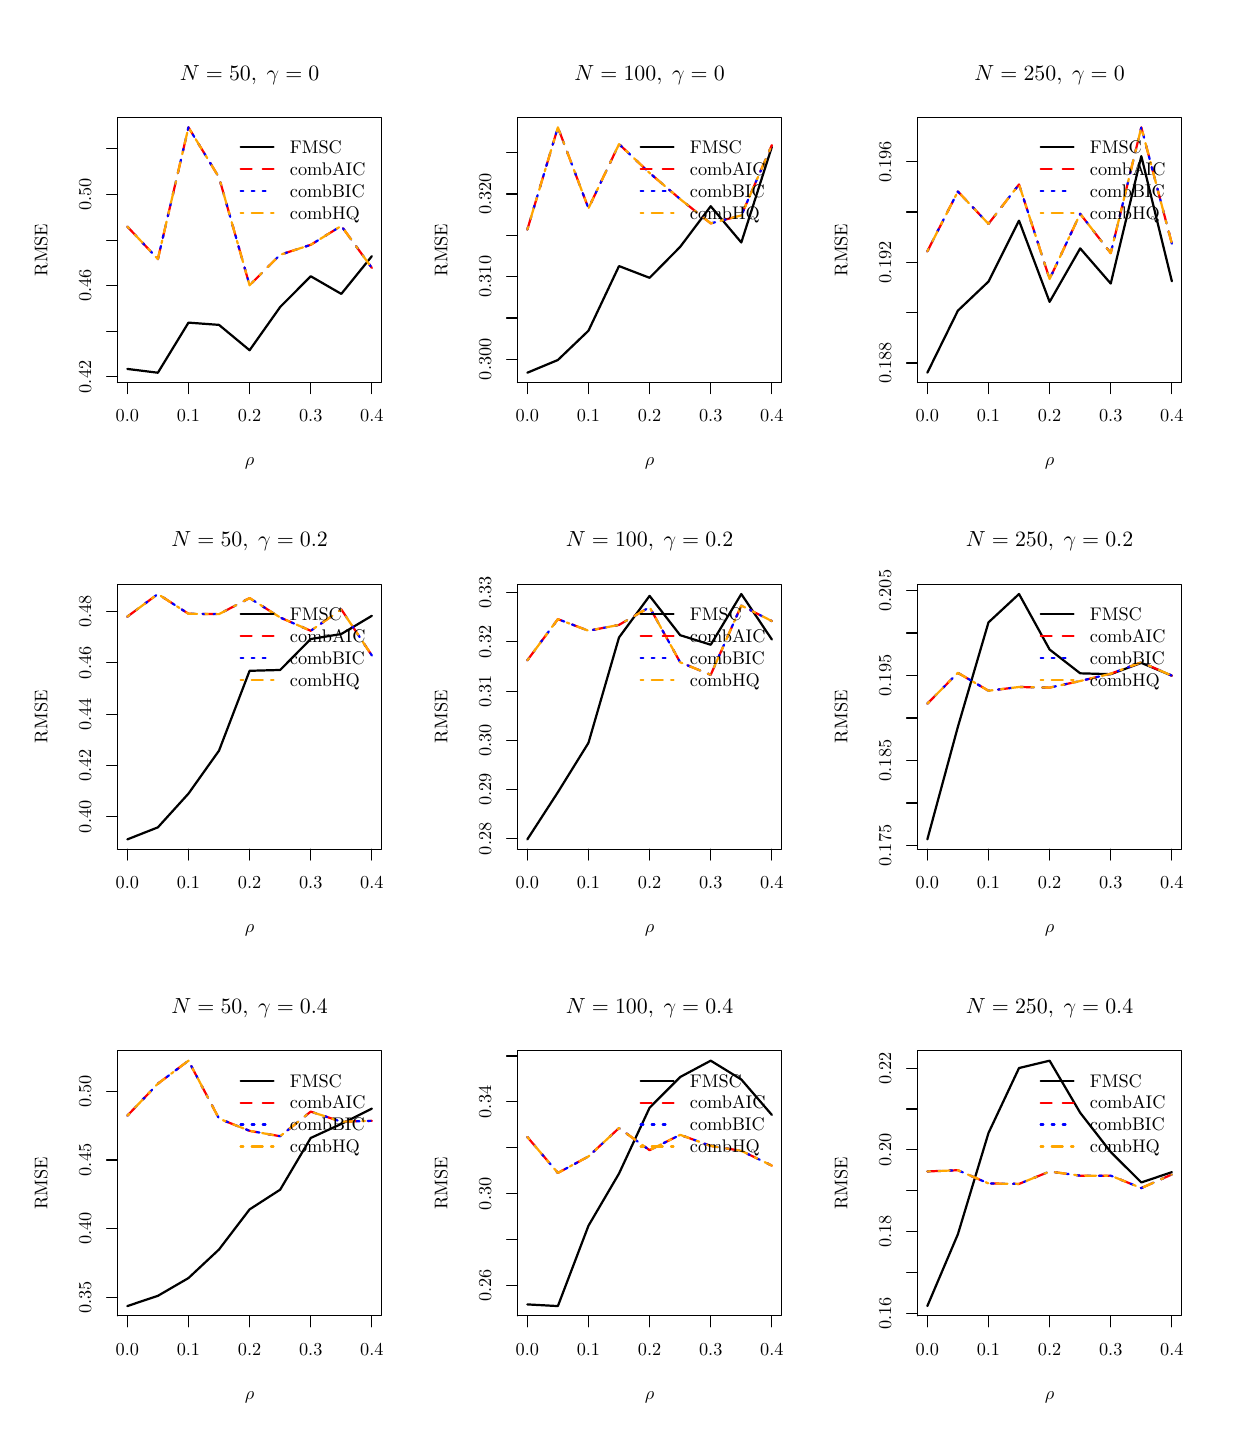
\begin{tikzpicture}[x=1pt,y=1pt]
\definecolor[named]{fillColor}{rgb}{1.00,1.00,1.00}
\path[use as bounding box,fill=fillColor,fill opacity=0.00] (0,0) rectangle (433.62,505.89);
\begin{scope}
\path[clip] ( 32.47,377.65) rectangle (127.91,473.42);
\definecolor[named]{drawColor}{rgb}{0.00,0.00,0.00}

\path[draw=drawColor,line width= 0.8pt,line join=round,line cap=round] ( 36.01,382.57) --
	( 47.05,381.20) --
	( 58.10,399.30) --
	( 69.14,398.49) --
	( 80.19,389.33) --
	( 91.24,404.95) --
	(102.28,416.06) --
	(113.33,409.68) --
	(124.37,423.32);
\end{scope}
\begin{scope}
\path[clip] (  0.00,  0.00) rectangle (433.62,505.89);
\definecolor[named]{drawColor}{rgb}{0.00,0.00,0.00}

\path[draw=drawColor,line width= 0.4pt,line join=round,line cap=round] ( 36.01,377.65) -- (124.37,377.65);

\path[draw=drawColor,line width= 0.4pt,line join=round,line cap=round] ( 36.01,377.65) -- ( 36.01,373.69);

\path[draw=drawColor,line width= 0.4pt,line join=round,line cap=round] ( 58.10,377.65) -- ( 58.10,373.69);

\path[draw=drawColor,line width= 0.4pt,line join=round,line cap=round] ( 80.19,377.65) -- ( 80.19,373.69);

\path[draw=drawColor,line width= 0.4pt,line join=round,line cap=round] (102.28,377.65) -- (102.28,373.69);

\path[draw=drawColor,line width= 0.4pt,line join=round,line cap=round] (124.37,377.65) -- (124.37,373.69);

\node[text=drawColor,anchor=base,inner sep=0pt, outer sep=0pt, scale=  0.66] at ( 36.01,363.40) {0.0};

\node[text=drawColor,anchor=base,inner sep=0pt, outer sep=0pt, scale=  0.66] at ( 58.10,363.40) {0.1};

\node[text=drawColor,anchor=base,inner sep=0pt, outer sep=0pt, scale=  0.66] at ( 80.19,363.40) {0.2};

\node[text=drawColor,anchor=base,inner sep=0pt, outer sep=0pt, scale=  0.66] at (102.28,363.40) {0.3};

\node[text=drawColor,anchor=base,inner sep=0pt, outer sep=0pt, scale=  0.66] at (124.37,363.40) {0.4};

\path[draw=drawColor,line width= 0.4pt,line join=round,line cap=round] ( 32.47,379.68) -- ( 32.47,462.08);

\path[draw=drawColor,line width= 0.4pt,line join=round,line cap=round] ( 32.47,379.68) -- ( 28.51,379.68);

\path[draw=drawColor,line width= 0.4pt,line join=round,line cap=round] ( 32.47,396.16) -- ( 28.51,396.16);

\path[draw=drawColor,line width= 0.4pt,line join=round,line cap=round] ( 32.47,412.64) -- ( 28.51,412.64);

\path[draw=drawColor,line width= 0.4pt,line join=round,line cap=round] ( 32.47,429.12) -- ( 28.51,429.12);

\path[draw=drawColor,line width= 0.4pt,line join=round,line cap=round] ( 32.47,445.60) -- ( 28.51,445.60);

\path[draw=drawColor,line width= 0.4pt,line join=round,line cap=round] ( 32.47,462.08) -- ( 28.51,462.08);

\node[text=drawColor,rotate= 90.00,anchor=base,inner sep=0pt, outer sep=0pt, scale=  0.66] at ( 22.97,379.68) {0.42};

\node[text=drawColor,rotate= 90.00,anchor=base,inner sep=0pt, outer sep=0pt, scale=  0.66] at ( 22.97,412.64) {0.46};

\node[text=drawColor,rotate= 90.00,anchor=base,inner sep=0pt, outer sep=0pt, scale=  0.66] at ( 22.97,445.60) {0.50};

\path[draw=drawColor,line width= 0.4pt,line join=round,line cap=round] ( 32.47,377.65) --
	(127.91,377.65) --
	(127.91,473.42) --
	( 32.47,473.42) --
	( 32.47,377.65);
\end{scope}
\begin{scope}
\path[clip] (  0.00,337.26) rectangle (144.54,505.89);
\definecolor[named]{drawColor}{rgb}{0.00,0.00,0.00}

\node[text=drawColor,anchor=base,inner sep=0pt, outer sep=0pt, scale=  0.79] at ( 80.19,486.92) {\bfseries $N=50, \;\gamma=0$};

\node[text=drawColor,anchor=base,inner sep=0pt, outer sep=0pt, scale=  0.66] at ( 80.19,347.56) {$\rho$};

\node[text=drawColor,rotate= 90.00,anchor=base,inner sep=0pt, outer sep=0pt, scale=  0.66] at (  7.13,425.53) {RMSE};
\end{scope}
\begin{scope}
\path[clip] ( 32.47,377.65) rectangle (127.91,473.42);
\definecolor[named]{drawColor}{rgb}{1.00,0.00,0.00}

\path[draw=drawColor,line width= 0.8pt,dash pattern=on 4pt off 4pt ,line join=round,line cap=round] ( 36.01,434.01) --
	( 47.05,422.27) --
	( 58.10,469.87) --
	( 69.14,451.78) --
	( 80.19,412.78) --
	( 91.24,423.83) --
	(102.28,427.41) --
	(113.33,434.25) --
	(124.37,419.07);
\definecolor[named]{drawColor}{rgb}{0.00,0.00,1.00}

\path[draw=drawColor,line width= 0.8pt,dash pattern=on 1pt off 3pt ,line join=round,line cap=round] ( 36.01,434.01) --
	( 47.05,422.27) --
	( 58.10,469.87) --
	( 69.14,451.78) --
	( 80.19,412.78) --
	( 91.24,423.83) --
	(102.28,427.41) --
	(113.33,434.25) --
	(124.37,419.07);
\definecolor[named]{drawColor}{rgb}{1.00,0.65,0.00}

\path[draw=drawColor,line width= 0.8pt,dash pattern=on 1pt off 3pt on 4pt off 3pt ,line join=round,line cap=round] ( 36.01,434.01) --
	( 47.05,422.27) --
	( 58.10,469.87) --
	( 69.14,451.78) --
	( 80.19,412.78) --
	( 91.24,423.83) --
	(102.28,427.41) --
	(113.33,434.25) --
	(124.37,419.07);
\definecolor[named]{drawColor}{rgb}{0.00,0.00,0.00}

\path[draw=drawColor,line width= 0.8pt,line join=round,line cap=round] ( 76.94,462.63) -- ( 88.82,462.63);
\definecolor[named]{drawColor}{rgb}{1.00,0.00,0.00}

\path[draw=drawColor,line width= 0.8pt,dash pattern=on 4pt off 4pt ,line join=round,line cap=round] ( 76.94,454.71) -- ( 88.82,454.71);
\definecolor[named]{drawColor}{rgb}{0.00,0.00,1.00}

\path[draw=drawColor,line width= 0.8pt,dash pattern=on 1pt off 3pt ,line join=round,line cap=round] ( 76.94,446.79) -- ( 88.82,446.79);
\definecolor[named]{drawColor}{rgb}{1.00,0.65,0.00}

\path[draw=drawColor,line width= 0.8pt,dash pattern=on 1pt off 3pt on 4pt off 3pt ,line join=round,line cap=round] ( 76.94,438.87) -- ( 88.82,438.87);
\definecolor[named]{drawColor}{rgb}{0.00,0.00,0.00}

\node[text=drawColor,anchor=base west,inner sep=0pt, outer sep=0pt, scale=  0.66] at ( 94.76,460.35) {FMSC};

\node[text=drawColor,anchor=base west,inner sep=0pt, outer sep=0pt, scale=  0.66] at ( 94.76,452.43) {combAIC};

\node[text=drawColor,anchor=base west,inner sep=0pt, outer sep=0pt, scale=  0.66] at ( 94.76,444.51) {combBIC};

\node[text=drawColor,anchor=base west,inner sep=0pt, outer sep=0pt, scale=  0.66] at ( 94.76,436.59) {combHQ};
\end{scope}
\begin{scope}
\path[clip] (177.01,377.65) rectangle (272.45,473.42);
\definecolor[named]{drawColor}{rgb}{0.00,0.00,0.00}

\path[draw=drawColor,line width= 0.8pt,line join=round,line cap=round] (180.55,381.20) --
	(191.59,385.80) --
	(202.64,396.38) --
	(213.68,419.74) --
	(224.73,415.49) --
	(235.78,426.69) --
	(246.82,441.36) --
	(257.87,428.26) --
	(268.91,462.83);
\end{scope}
\begin{scope}
\path[clip] (  0.00,  0.00) rectangle (433.62,505.89);
\definecolor[named]{drawColor}{rgb}{0.00,0.00,0.00}

\path[draw=drawColor,line width= 0.4pt,line join=round,line cap=round] (180.55,377.65) -- (268.91,377.65);

\path[draw=drawColor,line width= 0.4pt,line join=round,line cap=round] (180.55,377.65) -- (180.55,373.69);

\path[draw=drawColor,line width= 0.4pt,line join=round,line cap=round] (202.64,377.65) -- (202.64,373.69);

\path[draw=drawColor,line width= 0.4pt,line join=round,line cap=round] (224.73,377.65) -- (224.73,373.69);

\path[draw=drawColor,line width= 0.4pt,line join=round,line cap=round] (246.82,377.65) -- (246.82,373.69);

\path[draw=drawColor,line width= 0.4pt,line join=round,line cap=round] (268.91,377.65) -- (268.91,373.69);

\node[text=drawColor,anchor=base,inner sep=0pt, outer sep=0pt, scale=  0.66] at (180.55,363.40) {0.0};

\node[text=drawColor,anchor=base,inner sep=0pt, outer sep=0pt, scale=  0.66] at (202.64,363.40) {0.1};

\node[text=drawColor,anchor=base,inner sep=0pt, outer sep=0pt, scale=  0.66] at (224.73,363.40) {0.2};

\node[text=drawColor,anchor=base,inner sep=0pt, outer sep=0pt, scale=  0.66] at (246.82,363.40) {0.3};

\node[text=drawColor,anchor=base,inner sep=0pt, outer sep=0pt, scale=  0.66] at (268.91,363.40) {0.4};

\path[draw=drawColor,line width= 0.4pt,line join=round,line cap=round] (177.01,386.05) -- (177.01,460.74);

\path[draw=drawColor,line width= 0.4pt,line join=round,line cap=round] (177.01,386.05) -- (173.05,386.05);

\path[draw=drawColor,line width= 0.4pt,line join=round,line cap=round] (177.01,400.99) -- (173.05,400.99);

\path[draw=drawColor,line width= 0.4pt,line join=round,line cap=round] (177.01,415.92) -- (173.05,415.92);

\path[draw=drawColor,line width= 0.4pt,line join=round,line cap=round] (177.01,430.86) -- (173.05,430.86);

\path[draw=drawColor,line width= 0.4pt,line join=round,line cap=round] (177.01,445.80) -- (173.05,445.80);

\path[draw=drawColor,line width= 0.4pt,line join=round,line cap=round] (177.01,460.74) -- (173.05,460.74);

\node[text=drawColor,rotate= 90.00,anchor=base,inner sep=0pt, outer sep=0pt, scale=  0.66] at (167.51,386.05) {0.300};

\node[text=drawColor,rotate= 90.00,anchor=base,inner sep=0pt, outer sep=0pt, scale=  0.66] at (167.51,415.92) {0.310};

\node[text=drawColor,rotate= 90.00,anchor=base,inner sep=0pt, outer sep=0pt, scale=  0.66] at (167.51,445.80) {0.320};

\path[draw=drawColor,line width= 0.4pt,line join=round,line cap=round] (177.01,377.65) --
	(272.45,377.65) --
	(272.45,473.42) --
	(177.01,473.42) --
	(177.01,377.65);
\end{scope}
\begin{scope}
\path[clip] (144.54,337.26) rectangle (289.08,505.89);
\definecolor[named]{drawColor}{rgb}{0.00,0.00,0.00}

\node[text=drawColor,anchor=base,inner sep=0pt, outer sep=0pt, scale=  0.79] at (224.73,486.92) {\bfseries $N=100, \;\gamma=0$};

\node[text=drawColor,anchor=base,inner sep=0pt, outer sep=0pt, scale=  0.66] at (224.73,347.56) {$\rho$};

\node[text=drawColor,rotate= 90.00,anchor=base,inner sep=0pt, outer sep=0pt, scale=  0.66] at (151.67,425.54) {RMSE};
\end{scope}
\begin{scope}
\path[clip] (177.01,377.65) rectangle (272.45,473.42);
\definecolor[named]{drawColor}{rgb}{1.00,0.00,0.00}

\path[draw=drawColor,line width= 0.8pt,dash pattern=on 4pt off 4pt ,line join=round,line cap=round] (180.55,432.92) --
	(191.59,469.87) --
	(202.64,440.61) --
	(213.68,463.81) --
	(224.73,453.38) --
	(235.78,443.94) --
	(246.82,435.16) --
	(257.87,438.04) --
	(268.91,463.47);
\definecolor[named]{drawColor}{rgb}{0.00,0.00,1.00}

\path[draw=drawColor,line width= 0.8pt,dash pattern=on 1pt off 3pt ,line join=round,line cap=round] (180.55,432.92) --
	(191.59,469.87) --
	(202.64,440.61) --
	(213.68,463.81) --
	(224.73,453.38) --
	(235.78,443.94) --
	(246.82,435.16) --
	(257.87,438.04) --
	(268.91,463.47);
\definecolor[named]{drawColor}{rgb}{1.00,0.65,0.00}

\path[draw=drawColor,line width= 0.8pt,dash pattern=on 1pt off 3pt on 4pt off 3pt ,line join=round,line cap=round] (180.55,432.92) --
	(191.59,469.87) --
	(202.64,440.61) --
	(213.68,463.81) --
	(224.73,453.38) --
	(235.78,443.94) --
	(246.82,435.16) --
	(257.87,438.04) --
	(268.91,463.47);
\definecolor[named]{drawColor}{rgb}{0.00,0.00,0.00}

\path[draw=drawColor,line width= 0.8pt,line join=round,line cap=round] (221.48,462.63) -- (233.36,462.63);
\definecolor[named]{drawColor}{rgb}{1.00,0.00,0.00}

\path[draw=drawColor,line width= 0.8pt,dash pattern=on 4pt off 4pt ,line join=round,line cap=round] (221.48,454.71) -- (233.36,454.71);
\definecolor[named]{drawColor}{rgb}{0.00,0.00,1.00}

\path[draw=drawColor,line width= 0.8pt,dash pattern=on 1pt off 3pt ,line join=round,line cap=round] (221.48,446.79) -- (233.36,446.79);
\definecolor[named]{drawColor}{rgb}{1.00,0.65,0.00}

\path[draw=drawColor,line width= 0.8pt,dash pattern=on 1pt off 3pt on 4pt off 3pt ,line join=round,line cap=round] (221.48,438.87) -- (233.36,438.87);
\definecolor[named]{drawColor}{rgb}{0.00,0.00,0.00}

\node[text=drawColor,anchor=base west,inner sep=0pt, outer sep=0pt, scale=  0.66] at (239.30,460.35) {FMSC};

\node[text=drawColor,anchor=base west,inner sep=0pt, outer sep=0pt, scale=  0.66] at (239.30,452.43) {combAIC};

\node[text=drawColor,anchor=base west,inner sep=0pt, outer sep=0pt, scale=  0.66] at (239.30,444.51) {combBIC};

\node[text=drawColor,anchor=base west,inner sep=0pt, outer sep=0pt, scale=  0.66] at (239.30,436.59) {combHQ};
\end{scope}
\begin{scope}
\path[clip] (321.55,377.65) rectangle (416.99,473.42);
\definecolor[named]{drawColor}{rgb}{0.00,0.00,0.00}

\path[draw=drawColor,line width= 0.8pt,line join=round,line cap=round] (325.09,381.20) --
	(336.13,403.63) --
	(347.18,414.13) --
	(358.22,436.15) --
	(369.27,406.80) --
	(380.32,426.13) --
	(391.36,413.42) --
	(402.41,459.46) --
	(413.45,414.24);
\end{scope}
\begin{scope}
\path[clip] (  0.00,  0.00) rectangle (433.62,505.89);
\definecolor[named]{drawColor}{rgb}{0.00,0.00,0.00}

\path[draw=drawColor,line width= 0.4pt,line join=round,line cap=round] (325.09,377.65) -- (413.45,377.65);

\path[draw=drawColor,line width= 0.4pt,line join=round,line cap=round] (325.09,377.65) -- (325.09,373.69);

\path[draw=drawColor,line width= 0.4pt,line join=round,line cap=round] (347.18,377.65) -- (347.18,373.69);

\path[draw=drawColor,line width= 0.4pt,line join=round,line cap=round] (369.27,377.65) -- (369.27,373.69);

\path[draw=drawColor,line width= 0.4pt,line join=round,line cap=round] (391.36,377.65) -- (391.36,373.69);

\path[draw=drawColor,line width= 0.4pt,line join=round,line cap=round] (413.45,377.65) -- (413.45,373.69);

\node[text=drawColor,anchor=base,inner sep=0pt, outer sep=0pt, scale=  0.66] at (325.09,363.40) {0.0};

\node[text=drawColor,anchor=base,inner sep=0pt, outer sep=0pt, scale=  0.66] at (347.18,363.40) {0.1};

\node[text=drawColor,anchor=base,inner sep=0pt, outer sep=0pt, scale=  0.66] at (369.27,363.40) {0.2};

\node[text=drawColor,anchor=base,inner sep=0pt, outer sep=0pt, scale=  0.66] at (391.36,363.40) {0.3};

\node[text=drawColor,anchor=base,inner sep=0pt, outer sep=0pt, scale=  0.66] at (413.45,363.40) {0.4};

\path[draw=drawColor,line width= 0.4pt,line join=round,line cap=round] (321.55,384.73) -- (321.55,457.44);

\path[draw=drawColor,line width= 0.4pt,line join=round,line cap=round] (321.55,384.73) -- (317.59,384.73);

\path[draw=drawColor,line width= 0.4pt,line join=round,line cap=round] (321.55,402.91) -- (317.59,402.91);

\path[draw=drawColor,line width= 0.4pt,line join=round,line cap=round] (321.55,421.08) -- (317.59,421.08);

\path[draw=drawColor,line width= 0.4pt,line join=round,line cap=round] (321.55,439.26) -- (317.59,439.26);

\path[draw=drawColor,line width= 0.4pt,line join=round,line cap=round] (321.55,457.44) -- (317.59,457.44);

\node[text=drawColor,rotate= 90.00,anchor=base,inner sep=0pt, outer sep=0pt, scale=  0.66] at (312.05,384.73) {0.188};

\node[text=drawColor,rotate= 90.00,anchor=base,inner sep=0pt, outer sep=0pt, scale=  0.66] at (312.05,421.08) {0.192};

\node[text=drawColor,rotate= 90.00,anchor=base,inner sep=0pt, outer sep=0pt, scale=  0.66] at (312.05,457.44) {0.196};

\path[draw=drawColor,line width= 0.4pt,line join=round,line cap=round] (321.55,377.65) --
	(416.99,377.65) --
	(416.99,473.42) --
	(321.55,473.42) --
	(321.55,377.65);
\end{scope}
\begin{scope}
\path[clip] (289.08,337.26) rectangle (433.62,505.89);
\definecolor[named]{drawColor}{rgb}{0.00,0.00,0.00}

\node[text=drawColor,anchor=base,inner sep=0pt, outer sep=0pt, scale=  0.79] at (369.27,486.92) {\bfseries $N=250, \;\gamma=0$};

\node[text=drawColor,anchor=base,inner sep=0pt, outer sep=0pt, scale=  0.66] at (369.27,347.56) {$\rho$};

\node[text=drawColor,rotate= 90.00,anchor=base,inner sep=0pt, outer sep=0pt, scale=  0.66] at (296.21,425.53) {RMSE};
\end{scope}
\begin{scope}
\path[clip] (321.55,377.65) rectangle (416.99,473.42);
\definecolor[named]{drawColor}{rgb}{1.00,0.00,0.00}

\path[draw=drawColor,line width= 0.8pt,dash pattern=on 4pt off 4pt ,line join=round,line cap=round] (325.09,425.07) --
	(336.13,446.68) --
	(347.18,435.00) --
	(358.22,449.24) --
	(369.27,415.06) --
	(380.32,438.63) --
	(391.36,424.40) --
	(402.41,469.87) --
	(413.45,427.83);
\definecolor[named]{drawColor}{rgb}{0.00,0.00,1.00}

\path[draw=drawColor,line width= 0.8pt,dash pattern=on 1pt off 3pt ,line join=round,line cap=round] (325.09,425.07) --
	(336.13,446.68) --
	(347.18,435.00) --
	(358.22,449.24) --
	(369.27,415.06) --
	(380.32,438.63) --
	(391.36,424.40) --
	(402.41,469.87) --
	(413.45,427.83);
\definecolor[named]{drawColor}{rgb}{1.00,0.65,0.00}

\path[draw=drawColor,line width= 0.8pt,dash pattern=on 1pt off 3pt on 4pt off 3pt ,line join=round,line cap=round] (325.09,425.07) --
	(336.13,446.68) --
	(347.18,435.00) --
	(358.22,449.24) --
	(369.27,415.06) --
	(380.32,438.63) --
	(391.36,424.40) --
	(402.41,469.87) --
	(413.45,427.83);
\definecolor[named]{drawColor}{rgb}{0.00,0.00,0.00}

\path[draw=drawColor,line width= 0.8pt,line join=round,line cap=round] (366.02,462.63) -- (377.90,462.63);
\definecolor[named]{drawColor}{rgb}{1.00,0.00,0.00}

\path[draw=drawColor,line width= 0.8pt,dash pattern=on 4pt off 4pt ,line join=round,line cap=round] (366.02,454.71) -- (377.90,454.71);
\definecolor[named]{drawColor}{rgb}{0.00,0.00,1.00}

\path[draw=drawColor,line width= 0.8pt,dash pattern=on 1pt off 3pt ,line join=round,line cap=round] (366.02,446.79) -- (377.90,446.79);
\definecolor[named]{drawColor}{rgb}{1.00,0.65,0.00}

\path[draw=drawColor,line width= 0.8pt,dash pattern=on 1pt off 3pt on 4pt off 3pt ,line join=round,line cap=round] (366.02,438.87) -- (377.90,438.87);
\definecolor[named]{drawColor}{rgb}{0.00,0.00,0.00}

\node[text=drawColor,anchor=base west,inner sep=0pt, outer sep=0pt, scale=  0.66] at (383.84,460.35) {FMSC};

\node[text=drawColor,anchor=base west,inner sep=0pt, outer sep=0pt, scale=  0.66] at (383.84,452.43) {combAIC};

\node[text=drawColor,anchor=base west,inner sep=0pt, outer sep=0pt, scale=  0.66] at (383.84,444.51) {combBIC};

\node[text=drawColor,anchor=base west,inner sep=0pt, outer sep=0pt, scale=  0.66] at (383.84,436.59) {combHQ};
\end{scope}
\begin{scope}
\path[clip] ( 32.47,209.02) rectangle (127.91,304.79);
\definecolor[named]{drawColor}{rgb}{0.00,0.00,0.00}

\path[draw=drawColor,line width= 0.8pt,line join=round,line cap=round] ( 36.01,212.57) --
	( 47.05,216.92) --
	( 58.10,229.11) --
	( 69.14,244.64) --
	( 80.19,273.49) --
	( 91.24,273.79) --
	(102.28,284.97) --
	(113.33,286.79) --
	(124.37,293.36);
\end{scope}
\begin{scope}
\path[clip] (  0.00,  0.00) rectangle (433.62,505.89);
\definecolor[named]{drawColor}{rgb}{0.00,0.00,0.00}

\path[draw=drawColor,line width= 0.4pt,line join=round,line cap=round] ( 36.01,209.02) -- (124.37,209.02);

\path[draw=drawColor,line width= 0.4pt,line join=round,line cap=round] ( 36.01,209.02) -- ( 36.01,205.06);

\path[draw=drawColor,line width= 0.4pt,line join=round,line cap=round] ( 58.10,209.02) -- ( 58.10,205.06);

\path[draw=drawColor,line width= 0.4pt,line join=round,line cap=round] ( 80.19,209.02) -- ( 80.19,205.06);

\path[draw=drawColor,line width= 0.4pt,line join=round,line cap=round] (102.28,209.02) -- (102.28,205.06);

\path[draw=drawColor,line width= 0.4pt,line join=round,line cap=round] (124.37,209.02) -- (124.37,205.06);

\node[text=drawColor,anchor=base,inner sep=0pt, outer sep=0pt, scale=  0.66] at ( 36.01,194.77) {0.0};

\node[text=drawColor,anchor=base,inner sep=0pt, outer sep=0pt, scale=  0.66] at ( 58.10,194.77) {0.1};

\node[text=drawColor,anchor=base,inner sep=0pt, outer sep=0pt, scale=  0.66] at ( 80.19,194.77) {0.2};

\node[text=drawColor,anchor=base,inner sep=0pt, outer sep=0pt, scale=  0.66] at (102.28,194.77) {0.3};

\node[text=drawColor,anchor=base,inner sep=0pt, outer sep=0pt, scale=  0.66] at (124.37,194.77) {0.4};

\path[draw=drawColor,line width= 0.4pt,line join=round,line cap=round] ( 32.47,220.75) -- ( 32.47,294.93);

\path[draw=drawColor,line width= 0.4pt,line join=round,line cap=round] ( 32.47,220.75) -- ( 28.51,220.75);

\path[draw=drawColor,line width= 0.4pt,line join=round,line cap=round] ( 32.47,239.29) -- ( 28.51,239.29);

\path[draw=drawColor,line width= 0.4pt,line join=round,line cap=round] ( 32.47,257.84) -- ( 28.51,257.84);

\path[draw=drawColor,line width= 0.4pt,line join=round,line cap=round] ( 32.47,276.38) -- ( 28.51,276.38);

\path[draw=drawColor,line width= 0.4pt,line join=round,line cap=round] ( 32.47,294.93) -- ( 28.51,294.93);

\node[text=drawColor,rotate= 90.00,anchor=base,inner sep=0pt, outer sep=0pt, scale=  0.66] at ( 22.97,220.75) {0.40};

\node[text=drawColor,rotate= 90.00,anchor=base,inner sep=0pt, outer sep=0pt, scale=  0.66] at ( 22.97,239.29) {0.42};

\node[text=drawColor,rotate= 90.00,anchor=base,inner sep=0pt, outer sep=0pt, scale=  0.66] at ( 22.97,257.84) {0.44};

\node[text=drawColor,rotate= 90.00,anchor=base,inner sep=0pt, outer sep=0pt, scale=  0.66] at ( 22.97,276.38) {0.46};

\node[text=drawColor,rotate= 90.00,anchor=base,inner sep=0pt, outer sep=0pt, scale=  0.66] at ( 22.97,294.93) {0.48};

\path[draw=drawColor,line width= 0.4pt,line join=round,line cap=round] ( 32.47,209.02) --
	(127.91,209.02) --
	(127.91,304.79) --
	( 32.47,304.79) --
	( 32.47,209.02);
\end{scope}
\begin{scope}
\path[clip] (  0.00,168.63) rectangle (144.54,337.26);
\definecolor[named]{drawColor}{rgb}{0.00,0.00,0.00}

\node[text=drawColor,anchor=base,inner sep=0pt, outer sep=0pt, scale=  0.79] at ( 80.19,318.29) {\bfseries $N=50, \;\gamma=0.2$};

\node[text=drawColor,anchor=base,inner sep=0pt, outer sep=0pt, scale=  0.66] at ( 80.19,178.93) {$\rho$};

\node[text=drawColor,rotate= 90.00,anchor=base,inner sep=0pt, outer sep=0pt, scale=  0.66] at (  7.13,256.90) {RMSE};
\end{scope}
\begin{scope}
\path[clip] ( 32.47,209.02) rectangle (127.91,304.79);
\definecolor[named]{drawColor}{rgb}{1.00,0.00,0.00}

\path[draw=drawColor,line width= 0.8pt,dash pattern=on 4pt off 4pt ,line join=round,line cap=round] ( 36.01,293.06) --
	( 47.05,301.24) --
	( 58.10,294.10) --
	( 69.14,293.97) --
	( 80.19,299.77) --
	( 91.24,292.76) --
	(102.28,287.95) --
	(113.33,295.67) --
	(124.37,279.02);
\definecolor[named]{drawColor}{rgb}{0.00,0.00,1.00}

\path[draw=drawColor,line width= 0.8pt,dash pattern=on 1pt off 3pt ,line join=round,line cap=round] ( 36.01,293.06) --
	( 47.05,301.24) --
	( 58.10,294.10) --
	( 69.14,293.97) --
	( 80.19,299.77) --
	( 91.24,292.76) --
	(102.28,287.95) --
	(113.33,295.67) --
	(124.37,279.02);
\definecolor[named]{drawColor}{rgb}{1.00,0.65,0.00}

\path[draw=drawColor,line width= 0.8pt,dash pattern=on 1pt off 3pt on 4pt off 3pt ,line join=round,line cap=round] ( 36.01,293.06) --
	( 47.05,301.24) --
	( 58.10,294.10) --
	( 69.14,293.97) --
	( 80.19,299.77) --
	( 91.24,292.76) --
	(102.28,287.95) --
	(113.33,295.67) --
	(124.37,279.02);
\definecolor[named]{drawColor}{rgb}{0.00,0.00,0.00}

\path[draw=drawColor,line width= 0.8pt,line join=round,line cap=round] ( 76.94,294.00) -- ( 88.82,294.00);
\definecolor[named]{drawColor}{rgb}{1.00,0.00,0.00}

\path[draw=drawColor,line width= 0.8pt,dash pattern=on 4pt off 4pt ,line join=round,line cap=round] ( 76.94,286.08) -- ( 88.82,286.08);
\definecolor[named]{drawColor}{rgb}{0.00,0.00,1.00}

\path[draw=drawColor,line width= 0.8pt,dash pattern=on 1pt off 3pt ,line join=round,line cap=round] ( 76.94,278.16) -- ( 88.82,278.16);
\definecolor[named]{drawColor}{rgb}{1.00,0.65,0.00}

\path[draw=drawColor,line width= 0.8pt,dash pattern=on 1pt off 3pt on 4pt off 3pt ,line join=round,line cap=round] ( 76.94,270.24) -- ( 88.82,270.24);
\definecolor[named]{drawColor}{rgb}{0.00,0.00,0.00}

\node[text=drawColor,anchor=base west,inner sep=0pt, outer sep=0pt, scale=  0.66] at ( 94.76,291.72) {FMSC};

\node[text=drawColor,anchor=base west,inner sep=0pt, outer sep=0pt, scale=  0.66] at ( 94.76,283.80) {combAIC};

\node[text=drawColor,anchor=base west,inner sep=0pt, outer sep=0pt, scale=  0.66] at ( 94.76,275.88) {combBIC};

\node[text=drawColor,anchor=base west,inner sep=0pt, outer sep=0pt, scale=  0.66] at ( 94.76,267.96) {combHQ};
\end{scope}
\begin{scope}
\path[clip] (177.01,209.02) rectangle (272.45,304.79);
\definecolor[named]{drawColor}{rgb}{0.00,0.00,0.00}

\path[draw=drawColor,line width= 0.8pt,line join=round,line cap=round] (180.55,212.57) --
	(191.59,229.62) --
	(202.64,247.45) --
	(213.68,285.54) --
	(224.73,300.57) --
	(235.78,286.36) --
	(246.82,282.91) --
	(257.87,301.24) --
	(268.91,284.80);
\end{scope}
\begin{scope}
\path[clip] (  0.00,  0.00) rectangle (433.62,505.89);
\definecolor[named]{drawColor}{rgb}{0.00,0.00,0.00}

\path[draw=drawColor,line width= 0.4pt,line join=round,line cap=round] (180.55,209.02) -- (268.91,209.02);

\path[draw=drawColor,line width= 0.4pt,line join=round,line cap=round] (180.55,209.02) -- (180.55,205.06);

\path[draw=drawColor,line width= 0.4pt,line join=round,line cap=round] (202.64,209.02) -- (202.64,205.06);

\path[draw=drawColor,line width= 0.4pt,line join=round,line cap=round] (224.73,209.02) -- (224.73,205.06);

\path[draw=drawColor,line width= 0.4pt,line join=round,line cap=round] (246.82,209.02) -- (246.82,205.06);

\path[draw=drawColor,line width= 0.4pt,line join=round,line cap=round] (268.91,209.02) -- (268.91,205.06);

\node[text=drawColor,anchor=base,inner sep=0pt, outer sep=0pt, scale=  0.66] at (180.55,194.77) {0.0};

\node[text=drawColor,anchor=base,inner sep=0pt, outer sep=0pt, scale=  0.66] at (202.64,194.77) {0.1};

\node[text=drawColor,anchor=base,inner sep=0pt, outer sep=0pt, scale=  0.66] at (224.73,194.77) {0.2};

\node[text=drawColor,anchor=base,inner sep=0pt, outer sep=0pt, scale=  0.66] at (246.82,194.77) {0.3};

\node[text=drawColor,anchor=base,inner sep=0pt, outer sep=0pt, scale=  0.66] at (268.91,194.77) {0.4};

\path[draw=drawColor,line width= 0.4pt,line join=round,line cap=round] (177.01,212.80) -- (177.01,301.70);

\path[draw=drawColor,line width= 0.4pt,line join=round,line cap=round] (177.01,212.80) -- (173.05,212.80);

\path[draw=drawColor,line width= 0.4pt,line join=round,line cap=round] (177.01,230.58) -- (173.05,230.58);

\path[draw=drawColor,line width= 0.4pt,line join=round,line cap=round] (177.01,248.36) -- (173.05,248.36);

\path[draw=drawColor,line width= 0.4pt,line join=round,line cap=round] (177.01,266.14) -- (173.05,266.14);

\path[draw=drawColor,line width= 0.4pt,line join=round,line cap=round] (177.01,283.92) -- (173.05,283.92);

\path[draw=drawColor,line width= 0.4pt,line join=round,line cap=round] (177.01,301.70) -- (173.05,301.70);

\node[text=drawColor,rotate= 90.00,anchor=base,inner sep=0pt, outer sep=0pt, scale=  0.66] at (167.51,212.80) {0.28};

\node[text=drawColor,rotate= 90.00,anchor=base,inner sep=0pt, outer sep=0pt, scale=  0.66] at (167.51,230.58) {0.29};

\node[text=drawColor,rotate= 90.00,anchor=base,inner sep=0pt, outer sep=0pt, scale=  0.66] at (167.51,248.36) {0.30};

\node[text=drawColor,rotate= 90.00,anchor=base,inner sep=0pt, outer sep=0pt, scale=  0.66] at (167.51,266.14) {0.31};

\node[text=drawColor,rotate= 90.00,anchor=base,inner sep=0pt, outer sep=0pt, scale=  0.66] at (167.51,283.92) {0.32};

\node[text=drawColor,rotate= 90.00,anchor=base,inner sep=0pt, outer sep=0pt, scale=  0.66] at (167.51,301.70) {0.33};

\path[draw=drawColor,line width= 0.4pt,line join=round,line cap=round] (177.01,209.02) --
	(272.45,209.02) --
	(272.45,304.79) --
	(177.01,304.79) --
	(177.01,209.02);
\end{scope}
\begin{scope}
\path[clip] (144.54,168.63) rectangle (289.08,337.26);
\definecolor[named]{drawColor}{rgb}{0.00,0.00,0.00}

\node[text=drawColor,anchor=base,inner sep=0pt, outer sep=0pt, scale=  0.79] at (224.73,318.29) {\bfseries $N=100, \;\gamma=0.2$};

\node[text=drawColor,anchor=base,inner sep=0pt, outer sep=0pt, scale=  0.66] at (224.73,178.93) {$\rho$};

\node[text=drawColor,rotate= 90.00,anchor=base,inner sep=0pt, outer sep=0pt, scale=  0.66] at (151.67,256.90) {RMSE};
\end{scope}
\begin{scope}
\path[clip] (177.01,209.02) rectangle (272.45,304.79);
\definecolor[named]{drawColor}{rgb}{1.00,0.00,0.00}

\path[draw=drawColor,line width= 0.8pt,dash pattern=on 4pt off 4pt ,line join=round,line cap=round] (180.55,277.28) --
	(191.59,292.16) --
	(202.64,287.97) --
	(213.68,290.08) --
	(224.73,296.49) --
	(235.78,276.56) --
	(246.82,272.04) --
	(257.87,297.07) --
	(268.91,291.46);
\definecolor[named]{drawColor}{rgb}{0.00,0.00,1.00}

\path[draw=drawColor,line width= 0.8pt,dash pattern=on 1pt off 3pt ,line join=round,line cap=round] (180.55,277.28) --
	(191.59,292.16) --
	(202.64,287.97) --
	(213.68,290.08) --
	(224.73,296.49) --
	(235.78,276.56) --
	(246.82,272.04) --
	(257.87,297.07) --
	(268.91,291.46);
\definecolor[named]{drawColor}{rgb}{1.00,0.65,0.00}

\path[draw=drawColor,line width= 0.8pt,dash pattern=on 1pt off 3pt on 4pt off 3pt ,line join=round,line cap=round] (180.55,277.28) --
	(191.59,292.16) --
	(202.64,287.97) --
	(213.68,290.08) --
	(224.73,296.49) --
	(235.78,276.56) --
	(246.82,272.04) --
	(257.87,297.07) --
	(268.91,291.46);
\definecolor[named]{drawColor}{rgb}{0.00,0.00,0.00}

\path[draw=drawColor,line width= 0.8pt,line join=round,line cap=round] (221.48,294.00) -- (233.36,294.00);
\definecolor[named]{drawColor}{rgb}{1.00,0.00,0.00}

\path[draw=drawColor,line width= 0.8pt,dash pattern=on 4pt off 4pt ,line join=round,line cap=round] (221.48,286.08) -- (233.36,286.08);
\definecolor[named]{drawColor}{rgb}{0.00,0.00,1.00}

\path[draw=drawColor,line width= 0.8pt,dash pattern=on 1pt off 3pt ,line join=round,line cap=round] (221.48,278.16) -- (233.36,278.16);
\definecolor[named]{drawColor}{rgb}{1.00,0.65,0.00}

\path[draw=drawColor,line width= 0.8pt,dash pattern=on 1pt off 3pt on 4pt off 3pt ,line join=round,line cap=round] (221.48,270.24) -- (233.36,270.24);
\definecolor[named]{drawColor}{rgb}{0.00,0.00,0.00}

\node[text=drawColor,anchor=base west,inner sep=0pt, outer sep=0pt, scale=  0.66] at (239.30,291.72) {FMSC};

\node[text=drawColor,anchor=base west,inner sep=0pt, outer sep=0pt, scale=  0.66] at (239.30,283.80) {combAIC};

\node[text=drawColor,anchor=base west,inner sep=0pt, outer sep=0pt, scale=  0.66] at (239.30,275.88) {combBIC};

\node[text=drawColor,anchor=base west,inner sep=0pt, outer sep=0pt, scale=  0.66] at (239.30,267.96) {combHQ};
\end{scope}
\begin{scope}
\path[clip] (321.55,209.02) rectangle (416.99,304.79);
\definecolor[named]{drawColor}{rgb}{0.00,0.00,0.00}

\path[draw=drawColor,line width= 0.8pt,line join=round,line cap=round] (325.09,212.57) --
	(336.13,253.26) --
	(347.18,290.98) --
	(358.22,301.24) --
	(369.27,281.18) --
	(380.32,272.58) --
	(391.36,272.27) --
	(402.41,276.35) --
	(413.45,271.73);
\end{scope}
\begin{scope}
\path[clip] (  0.00,  0.00) rectangle (433.62,505.89);
\definecolor[named]{drawColor}{rgb}{0.00,0.00,0.00}

\path[draw=drawColor,line width= 0.4pt,line join=round,line cap=round] (325.09,209.02) -- (413.45,209.02);

\path[draw=drawColor,line width= 0.4pt,line join=round,line cap=round] (325.09,209.02) -- (325.09,205.06);

\path[draw=drawColor,line width= 0.4pt,line join=round,line cap=round] (347.18,209.02) -- (347.18,205.06);

\path[draw=drawColor,line width= 0.4pt,line join=round,line cap=round] (369.27,209.02) -- (369.27,205.06);

\path[draw=drawColor,line width= 0.4pt,line join=round,line cap=round] (391.36,209.02) -- (391.36,205.06);

\path[draw=drawColor,line width= 0.4pt,line join=round,line cap=round] (413.45,209.02) -- (413.45,205.06);

\node[text=drawColor,anchor=base,inner sep=0pt, outer sep=0pt, scale=  0.66] at (325.09,194.77) {0.0};

\node[text=drawColor,anchor=base,inner sep=0pt, outer sep=0pt, scale=  0.66] at (347.18,194.77) {0.1};

\node[text=drawColor,anchor=base,inner sep=0pt, outer sep=0pt, scale=  0.66] at (369.27,194.77) {0.2};

\node[text=drawColor,anchor=base,inner sep=0pt, outer sep=0pt, scale=  0.66] at (391.36,194.77) {0.3};

\node[text=drawColor,anchor=base,inner sep=0pt, outer sep=0pt, scale=  0.66] at (413.45,194.77) {0.4};

\path[draw=drawColor,line width= 0.4pt,line join=round,line cap=round] (321.55,210.39) -- (321.55,302.49);

\path[draw=drawColor,line width= 0.4pt,line join=round,line cap=round] (321.55,210.39) -- (317.59,210.39);

\path[draw=drawColor,line width= 0.4pt,line join=round,line cap=round] (321.55,225.74) -- (317.59,225.74);

\path[draw=drawColor,line width= 0.4pt,line join=round,line cap=round] (321.55,241.09) -- (317.59,241.09);

\path[draw=drawColor,line width= 0.4pt,line join=round,line cap=round] (321.55,256.44) -- (317.59,256.44);

\path[draw=drawColor,line width= 0.4pt,line join=round,line cap=round] (321.55,271.79) -- (317.59,271.79);

\path[draw=drawColor,line width= 0.4pt,line join=round,line cap=round] (321.55,287.14) -- (317.59,287.14);

\path[draw=drawColor,line width= 0.4pt,line join=round,line cap=round] (321.55,302.49) -- (317.59,302.49);

\node[text=drawColor,rotate= 90.00,anchor=base,inner sep=0pt, outer sep=0pt, scale=  0.66] at (312.05,210.39) {0.175};

\node[text=drawColor,rotate= 90.00,anchor=base,inner sep=0pt, outer sep=0pt, scale=  0.66] at (312.05,241.09) {0.185};

\node[text=drawColor,rotate= 90.00,anchor=base,inner sep=0pt, outer sep=0pt, scale=  0.66] at (312.05,271.79) {0.195};

\node[text=drawColor,rotate= 90.00,anchor=base,inner sep=0pt, outer sep=0pt, scale=  0.66] at (312.05,302.49) {0.205};

\path[draw=drawColor,line width= 0.4pt,line join=round,line cap=round] (321.55,209.02) --
	(416.99,209.02) --
	(416.99,304.79) --
	(321.55,304.79) --
	(321.55,209.02);
\end{scope}
\begin{scope}
\path[clip] (289.08,168.63) rectangle (433.62,337.26);
\definecolor[named]{drawColor}{rgb}{0.00,0.00,0.00}

\node[text=drawColor,anchor=base,inner sep=0pt, outer sep=0pt, scale=  0.79] at (369.27,318.29) {\bfseries $N=250, \;\gamma=0.2$};

\node[text=drawColor,anchor=base,inner sep=0pt, outer sep=0pt, scale=  0.66] at (369.27,178.93) {$\rho$};

\node[text=drawColor,rotate= 90.00,anchor=base,inner sep=0pt, outer sep=0pt, scale=  0.66] at (296.21,256.90) {RMSE};
\end{scope}
\begin{scope}
\path[clip] (321.55,209.02) rectangle (416.99,304.79);
\definecolor[named]{drawColor}{rgb}{1.00,0.00,0.00}

\path[draw=drawColor,line width= 0.8pt,dash pattern=on 4pt off 4pt ,line join=round,line cap=round] (325.09,261.62) --
	(336.13,272.76) --
	(347.18,266.29) --
	(358.22,267.64) --
	(369.27,267.41) --
	(380.32,269.80) --
	(391.36,272.43) --
	(402.41,276.55) --
	(413.45,271.74);
\definecolor[named]{drawColor}{rgb}{0.00,0.00,1.00}

\path[draw=drawColor,line width= 0.8pt,dash pattern=on 1pt off 3pt ,line join=round,line cap=round] (325.09,261.62) --
	(336.13,272.76) --
	(347.18,266.29) --
	(358.22,267.64) --
	(369.27,267.41) --
	(380.32,269.80) --
	(391.36,272.43) --
	(402.41,276.55) --
	(413.45,271.74);
\definecolor[named]{drawColor}{rgb}{1.00,0.65,0.00}

\path[draw=drawColor,line width= 0.8pt,dash pattern=on 1pt off 3pt on 4pt off 3pt ,line join=round,line cap=round] (325.09,261.62) --
	(336.13,272.76) --
	(347.18,266.29) --
	(358.22,267.64) --
	(369.27,267.41) --
	(380.32,269.80) --
	(391.36,272.43) --
	(402.41,276.55) --
	(413.45,271.74);
\definecolor[named]{drawColor}{rgb}{0.00,0.00,0.00}

\path[draw=drawColor,line width= 0.8pt,line join=round,line cap=round] (366.02,294.00) -- (377.90,294.00);
\definecolor[named]{drawColor}{rgb}{1.00,0.00,0.00}

\path[draw=drawColor,line width= 0.8pt,dash pattern=on 4pt off 4pt ,line join=round,line cap=round] (366.02,286.08) -- (377.90,286.08);
\definecolor[named]{drawColor}{rgb}{0.00,0.00,1.00}

\path[draw=drawColor,line width= 0.8pt,dash pattern=on 1pt off 3pt ,line join=round,line cap=round] (366.02,278.16) -- (377.90,278.16);
\definecolor[named]{drawColor}{rgb}{1.00,0.65,0.00}

\path[draw=drawColor,line width= 0.8pt,dash pattern=on 1pt off 3pt on 4pt off 3pt ,line join=round,line cap=round] (366.02,270.24) -- (377.90,270.24);
\definecolor[named]{drawColor}{rgb}{0.00,0.00,0.00}

\node[text=drawColor,anchor=base west,inner sep=0pt, outer sep=0pt, scale=  0.66] at (383.84,291.72) {FMSC};

\node[text=drawColor,anchor=base west,inner sep=0pt, outer sep=0pt, scale=  0.66] at (383.84,283.80) {combAIC};

\node[text=drawColor,anchor=base west,inner sep=0pt, outer sep=0pt, scale=  0.66] at (383.84,275.88) {combBIC};

\node[text=drawColor,anchor=base west,inner sep=0pt, outer sep=0pt, scale=  0.66] at (383.84,267.96) {combHQ};
\end{scope}
\begin{scope}
\path[clip] ( 32.47, 40.39) rectangle (127.91,136.16);
\definecolor[named]{drawColor}{rgb}{0.00,0.00,0.00}

\path[draw=drawColor,line width= 0.8pt,line join=round,line cap=round] ( 36.01, 43.94) --
	( 47.05, 47.64) --
	( 58.10, 54.06) --
	( 69.14, 64.39) --
	( 80.19, 78.87) --
	( 91.24, 86.00) --
	(102.28,104.68) --
	(113.33,109.76) --
	(124.37,115.30);
\end{scope}
\begin{scope}
\path[clip] (  0.00,  0.00) rectangle (433.62,505.89);
\definecolor[named]{drawColor}{rgb}{0.00,0.00,0.00}

\path[draw=drawColor,line width= 0.4pt,line join=round,line cap=round] ( 36.01, 40.39) -- (124.37, 40.39);

\path[draw=drawColor,line width= 0.4pt,line join=round,line cap=round] ( 36.01, 40.39) -- ( 36.01, 36.43);

\path[draw=drawColor,line width= 0.4pt,line join=round,line cap=round] ( 58.10, 40.39) -- ( 58.10, 36.43);

\path[draw=drawColor,line width= 0.4pt,line join=round,line cap=round] ( 80.19, 40.39) -- ( 80.19, 36.43);

\path[draw=drawColor,line width= 0.4pt,line join=round,line cap=round] (102.28, 40.39) -- (102.28, 36.43);

\path[draw=drawColor,line width= 0.4pt,line join=round,line cap=round] (124.37, 40.39) -- (124.37, 36.43);

\node[text=drawColor,anchor=base,inner sep=0pt, outer sep=0pt, scale=  0.66] at ( 36.01, 26.14) {0.0};

\node[text=drawColor,anchor=base,inner sep=0pt, outer sep=0pt, scale=  0.66] at ( 58.10, 26.14) {0.1};

\node[text=drawColor,anchor=base,inner sep=0pt, outer sep=0pt, scale=  0.66] at ( 80.19, 26.14) {0.2};

\node[text=drawColor,anchor=base,inner sep=0pt, outer sep=0pt, scale=  0.66] at (102.28, 26.14) {0.3};

\node[text=drawColor,anchor=base,inner sep=0pt, outer sep=0pt, scale=  0.66] at (124.37, 26.14) {0.4};

\path[draw=drawColor,line width= 0.4pt,line join=round,line cap=round] ( 32.47, 47.06) -- ( 32.47,121.59);

\path[draw=drawColor,line width= 0.4pt,line join=round,line cap=round] ( 32.47, 47.06) -- ( 28.51, 47.06);

\path[draw=drawColor,line width= 0.4pt,line join=round,line cap=round] ( 32.47, 71.90) -- ( 28.51, 71.90);

\path[draw=drawColor,line width= 0.4pt,line join=round,line cap=round] ( 32.47, 96.74) -- ( 28.51, 96.74);

\path[draw=drawColor,line width= 0.4pt,line join=round,line cap=round] ( 32.47,121.59) -- ( 28.51,121.59);

\node[text=drawColor,rotate= 90.00,anchor=base,inner sep=0pt, outer sep=0pt, scale=  0.66] at ( 22.97, 47.06) {0.35};

\node[text=drawColor,rotate= 90.00,anchor=base,inner sep=0pt, outer sep=0pt, scale=  0.66] at ( 22.97, 71.90) {0.40};

\node[text=drawColor,rotate= 90.00,anchor=base,inner sep=0pt, outer sep=0pt, scale=  0.66] at ( 22.97, 96.74) {0.45};

\node[text=drawColor,rotate= 90.00,anchor=base,inner sep=0pt, outer sep=0pt, scale=  0.66] at ( 22.97,121.59) {0.50};

\path[draw=drawColor,line width= 0.4pt,line join=round,line cap=round] ( 32.47, 40.39) --
	(127.91, 40.39) --
	(127.91,136.16) --
	( 32.47,136.16) --
	( 32.47, 40.39);
\end{scope}
\begin{scope}
\path[clip] (  0.00,  0.00) rectangle (144.54,168.63);
\definecolor[named]{drawColor}{rgb}{0.00,0.00,0.00}

\node[text=drawColor,anchor=base,inner sep=0pt, outer sep=0pt, scale=  0.79] at ( 80.19,149.66) {\bfseries $N=50, \;\gamma=0.4$};

\node[text=drawColor,anchor=base,inner sep=0pt, outer sep=0pt, scale=  0.66] at ( 80.19, 10.30) {$\rho$};

\node[text=drawColor,rotate= 90.00,anchor=base,inner sep=0pt, outer sep=0pt, scale=  0.66] at (  7.13, 88.27) {RMSE};
\end{scope}
\begin{scope}
\path[clip] ( 32.47, 40.39) rectangle (127.91,136.16);
\definecolor[named]{drawColor}{rgb}{1.00,0.00,0.00}

\path[draw=drawColor,line width= 0.8pt,dash pattern=on 4pt off 4pt ,line join=round,line cap=round] ( 36.01,112.73) --
	( 47.05,124.29) --
	( 58.10,132.61) --
	( 69.14,111.67) --
	( 80.19,107.26) --
	( 91.24,105.31) --
	(102.28,114.21) --
	(113.33,110.56) --
	(124.37,110.88);
\definecolor[named]{drawColor}{rgb}{0.00,0.00,1.00}

\path[draw=drawColor,line width= 0.8pt,dash pattern=on 1pt off 3pt ,line join=round,line cap=round] ( 36.01,112.73) --
	( 47.05,124.29) --
	( 58.10,132.61) --
	( 69.14,111.67) --
	( 80.19,107.26) --
	( 91.24,105.31) --
	(102.28,114.21) --
	(113.33,110.56) --
	(124.37,110.88);
\definecolor[named]{drawColor}{rgb}{1.00,0.65,0.00}

\path[draw=drawColor,line width= 0.8pt,dash pattern=on 1pt off 3pt on 4pt off 3pt ,line join=round,line cap=round] ( 36.01,112.73) --
	( 47.05,124.29) --
	( 58.10,132.61) --
	( 69.14,111.67) --
	( 80.19,107.26) --
	( 91.24,105.31) --
	(102.28,114.21) --
	(113.33,110.56) --
	(124.37,110.88);
\definecolor[named]{drawColor}{rgb}{0.00,0.00,0.00}

\path[draw=drawColor,line width= 0.8pt,line join=round,line cap=round] ( 76.94,125.37) -- ( 88.82,125.37);
\definecolor[named]{drawColor}{rgb}{1.00,0.00,0.00}

\path[draw=drawColor,line width= 0.8pt,dash pattern=on 4pt off 4pt ,line join=round,line cap=round] ( 76.94,117.45) -- ( 88.82,117.45);
\definecolor[named]{drawColor}{rgb}{0.00,0.00,1.00}

\path[draw=drawColor,line width= 0.8pt,dash pattern=on 1pt off 3pt ,line join=round,line cap=round] ( 76.94,109.53) -- ( 88.82,109.53);
\definecolor[named]{drawColor}{rgb}{1.00,0.65,0.00}

\path[draw=drawColor,line width= 0.8pt,dash pattern=on 1pt off 3pt on 4pt off 3pt ,line join=round,line cap=round] ( 76.94,101.61) -- ( 88.82,101.61);
\definecolor[named]{drawColor}{rgb}{0.00,0.00,0.00}

\node[text=drawColor,anchor=base west,inner sep=0pt, outer sep=0pt, scale=  0.66] at ( 94.76,123.09) {FMSC};

\node[text=drawColor,anchor=base west,inner sep=0pt, outer sep=0pt, scale=  0.66] at ( 94.76,115.17) {combAIC};

\node[text=drawColor,anchor=base west,inner sep=0pt, outer sep=0pt, scale=  0.66] at ( 94.76,107.25) {combBIC};

\node[text=drawColor,anchor=base west,inner sep=0pt, outer sep=0pt, scale=  0.66] at ( 94.76, 99.33) {combHQ};
\end{scope}
\begin{scope}
\path[clip] (177.01, 40.39) rectangle (272.45,136.16);
\definecolor[named]{drawColor}{rgb}{0.00,0.00,0.00}

\path[draw=drawColor,line width= 0.8pt,line join=round,line cap=round] (180.55, 44.54) --
	(191.59, 43.94) --
	(202.64, 72.97) --
	(213.68, 91.83) --
	(224.73,115.61) --
	(235.78,126.71) --
	(246.82,132.61) --
	(257.87,125.82) --
	(268.91,113.01);
\end{scope}
\begin{scope}
\path[clip] (  0.00,  0.00) rectangle (433.62,505.89);
\definecolor[named]{drawColor}{rgb}{0.00,0.00,0.00}

\path[draw=drawColor,line width= 0.4pt,line join=round,line cap=round] (180.55, 40.39) -- (268.91, 40.39);

\path[draw=drawColor,line width= 0.4pt,line join=round,line cap=round] (180.55, 40.39) -- (180.55, 36.43);

\path[draw=drawColor,line width= 0.4pt,line join=round,line cap=round] (202.64, 40.39) -- (202.64, 36.43);

\path[draw=drawColor,line width= 0.4pt,line join=round,line cap=round] (224.73, 40.39) -- (224.73, 36.43);

\path[draw=drawColor,line width= 0.4pt,line join=round,line cap=round] (246.82, 40.39) -- (246.82, 36.43);

\path[draw=drawColor,line width= 0.4pt,line join=round,line cap=round] (268.91, 40.39) -- (268.91, 36.43);

\node[text=drawColor,anchor=base,inner sep=0pt, outer sep=0pt, scale=  0.66] at (180.55, 26.14) {0.0};

\node[text=drawColor,anchor=base,inner sep=0pt, outer sep=0pt, scale=  0.66] at (202.64, 26.14) {0.1};

\node[text=drawColor,anchor=base,inner sep=0pt, outer sep=0pt, scale=  0.66] at (224.73, 26.14) {0.2};

\node[text=drawColor,anchor=base,inner sep=0pt, outer sep=0pt, scale=  0.66] at (246.82, 26.14) {0.3};

\node[text=drawColor,anchor=base,inner sep=0pt, outer sep=0pt, scale=  0.66] at (268.91, 26.14) {0.4};

\path[draw=drawColor,line width= 0.4pt,line join=round,line cap=round] (177.01, 51.34) -- (177.01,134.30);

\path[draw=drawColor,line width= 0.4pt,line join=round,line cap=round] (177.01, 51.34) -- (173.05, 51.34);

\path[draw=drawColor,line width= 0.4pt,line join=round,line cap=round] (177.01, 67.93) -- (173.05, 67.93);

\path[draw=drawColor,line width= 0.4pt,line join=round,line cap=round] (177.01, 84.52) -- (173.05, 84.52);

\path[draw=drawColor,line width= 0.4pt,line join=round,line cap=round] (177.01,101.12) -- (173.05,101.12);

\path[draw=drawColor,line width= 0.4pt,line join=round,line cap=round] (177.01,117.71) -- (173.05,117.71);

\path[draw=drawColor,line width= 0.4pt,line join=round,line cap=round] (177.01,134.30) -- (173.05,134.30);

\node[text=drawColor,rotate= 90.00,anchor=base,inner sep=0pt, outer sep=0pt, scale=  0.66] at (167.51, 51.34) {0.26};

\node[text=drawColor,rotate= 90.00,anchor=base,inner sep=0pt, outer sep=0pt, scale=  0.66] at (167.51, 84.52) {0.30};

\node[text=drawColor,rotate= 90.00,anchor=base,inner sep=0pt, outer sep=0pt, scale=  0.66] at (167.51,117.71) {0.34};

\path[draw=drawColor,line width= 0.4pt,line join=round,line cap=round] (177.01, 40.39) --
	(272.45, 40.39) --
	(272.45,136.16) --
	(177.01,136.16) --
	(177.01, 40.39);
\end{scope}
\begin{scope}
\path[clip] (144.54,  0.00) rectangle (289.08,168.63);
\definecolor[named]{drawColor}{rgb}{0.00,0.00,0.00}

\node[text=drawColor,anchor=base,inner sep=0pt, outer sep=0pt, scale=  0.79] at (224.73,149.66) {\bfseries $N=100, \;\gamma=0.4$};

\node[text=drawColor,anchor=base,inner sep=0pt, outer sep=0pt, scale=  0.66] at (224.73, 10.30) {$\rho$};

\node[text=drawColor,rotate= 90.00,anchor=base,inner sep=0pt, outer sep=0pt, scale=  0.66] at (151.67, 88.27) {RMSE};
\end{scope}
\begin{scope}
\path[clip] (177.01, 40.39) rectangle (272.45,136.16);
\definecolor[named]{drawColor}{rgb}{1.00,0.00,0.00}

\path[draw=drawColor,line width= 0.8pt,dash pattern=on 4pt off 4pt ,line join=round,line cap=round] (180.55,105.04) --
	(191.59, 92.05) --
	(202.64, 98.00) --
	(213.68,108.26) --
	(224.73,100.27) --
	(235.78,105.82) --
	(246.82,101.81) --
	(257.87,100.04) --
	(268.91, 94.70);
\definecolor[named]{drawColor}{rgb}{0.00,0.00,1.00}

\path[draw=drawColor,line width= 0.8pt,dash pattern=on 1pt off 3pt ,line join=round,line cap=round] (180.55,105.04) --
	(191.59, 92.05) --
	(202.64, 98.00) --
	(213.68,108.26) --
	(224.73,100.27) --
	(235.78,105.82) --
	(246.82,101.81) --
	(257.87,100.04) --
	(268.91, 94.70);
\definecolor[named]{drawColor}{rgb}{1.00,0.65,0.00}

\path[draw=drawColor,line width= 0.8pt,dash pattern=on 1pt off 3pt on 4pt off 3pt ,line join=round,line cap=round] (180.55,105.04) --
	(191.59, 92.05) --
	(202.64, 98.00) --
	(213.68,108.26) --
	(224.73,100.27) --
	(235.78,105.82) --
	(246.82,101.81) --
	(257.87,100.04) --
	(268.91, 94.70);
\definecolor[named]{drawColor}{rgb}{0.00,0.00,0.00}

\path[draw=drawColor,line width= 0.8pt,line join=round,line cap=round] (221.48,125.37) -- (233.36,125.37);
\definecolor[named]{drawColor}{rgb}{1.00,0.00,0.00}

\path[draw=drawColor,line width= 0.8pt,dash pattern=on 4pt off 4pt ,line join=round,line cap=round] (221.48,117.45) -- (233.36,117.45);
\definecolor[named]{drawColor}{rgb}{0.00,0.00,1.00}

\path[draw=drawColor,line width= 0.8pt,dash pattern=on 1pt off 3pt ,line join=round,line cap=round] (221.48,109.53) -- (233.36,109.53);
\definecolor[named]{drawColor}{rgb}{1.00,0.65,0.00}

\path[draw=drawColor,line width= 0.8pt,dash pattern=on 1pt off 3pt on 4pt off 3pt ,line join=round,line cap=round] (221.48,101.61) -- (233.36,101.61);
\definecolor[named]{drawColor}{rgb}{0.00,0.00,0.00}

\node[text=drawColor,anchor=base west,inner sep=0pt, outer sep=0pt, scale=  0.66] at (239.30,123.09) {FMSC};

\node[text=drawColor,anchor=base west,inner sep=0pt, outer sep=0pt, scale=  0.66] at (239.30,115.17) {combAIC};

\node[text=drawColor,anchor=base west,inner sep=0pt, outer sep=0pt, scale=  0.66] at (239.30,107.25) {combBIC};

\node[text=drawColor,anchor=base west,inner sep=0pt, outer sep=0pt, scale=  0.66] at (239.30, 99.33) {combHQ};
\end{scope}
\begin{scope}
\path[clip] (321.55, 40.39) rectangle (416.99,136.16);
\definecolor[named]{drawColor}{rgb}{0.00,0.00,0.00}

\path[draw=drawColor,line width= 0.8pt,line join=round,line cap=round] (325.09, 43.94) --
	(336.13, 69.90) --
	(347.18,106.46) --
	(358.22,129.95) --
	(369.27,132.61) --
	(380.32,113.80) --
	(391.36, 99.62) --
	(402.41, 88.61) --
	(413.45, 92.33);
\end{scope}
\begin{scope}
\path[clip] (  0.00,  0.00) rectangle (433.62,505.89);
\definecolor[named]{drawColor}{rgb}{0.00,0.00,0.00}

\path[draw=drawColor,line width= 0.4pt,line join=round,line cap=round] (325.09, 40.39) -- (413.45, 40.39);

\path[draw=drawColor,line width= 0.4pt,line join=round,line cap=round] (325.09, 40.39) -- (325.09, 36.43);

\path[draw=drawColor,line width= 0.4pt,line join=round,line cap=round] (347.18, 40.39) -- (347.18, 36.43);

\path[draw=drawColor,line width= 0.4pt,line join=round,line cap=round] (369.27, 40.39) -- (369.27, 36.43);

\path[draw=drawColor,line width= 0.4pt,line join=round,line cap=round] (391.36, 40.39) -- (391.36, 36.43);

\path[draw=drawColor,line width= 0.4pt,line join=round,line cap=round] (413.45, 40.39) -- (413.45, 36.43);

\node[text=drawColor,anchor=base,inner sep=0pt, outer sep=0pt, scale=  0.66] at (325.09, 26.14) {0.0};

\node[text=drawColor,anchor=base,inner sep=0pt, outer sep=0pt, scale=  0.66] at (347.18, 26.14) {0.1};

\node[text=drawColor,anchor=base,inner sep=0pt, outer sep=0pt, scale=  0.66] at (369.27, 26.14) {0.2};

\node[text=drawColor,anchor=base,inner sep=0pt, outer sep=0pt, scale=  0.66] at (391.36, 26.14) {0.3};

\node[text=drawColor,anchor=base,inner sep=0pt, outer sep=0pt, scale=  0.66] at (413.45, 26.14) {0.4};

\path[draw=drawColor,line width= 0.4pt,line join=round,line cap=round] (321.55, 41.29) -- (321.55,129.92);

\path[draw=drawColor,line width= 0.4pt,line join=round,line cap=round] (321.55, 41.29) -- (317.59, 41.29);

\path[draw=drawColor,line width= 0.4pt,line join=round,line cap=round] (321.55, 56.06) -- (317.59, 56.06);

\path[draw=drawColor,line width= 0.4pt,line join=round,line cap=round] (321.55, 70.83) -- (317.59, 70.83);

\path[draw=drawColor,line width= 0.4pt,line join=round,line cap=round] (321.55, 85.60) -- (317.59, 85.60);

\path[draw=drawColor,line width= 0.4pt,line join=round,line cap=round] (321.55,100.37) -- (317.59,100.37);

\path[draw=drawColor,line width= 0.4pt,line join=round,line cap=round] (321.55,115.15) -- (317.59,115.15);

\path[draw=drawColor,line width= 0.4pt,line join=round,line cap=round] (321.55,129.92) -- (317.59,129.92);

\node[text=drawColor,rotate= 90.00,anchor=base,inner sep=0pt, outer sep=0pt, scale=  0.66] at (312.05, 41.29) {0.16};

\node[text=drawColor,rotate= 90.00,anchor=base,inner sep=0pt, outer sep=0pt, scale=  0.66] at (312.05, 70.83) {0.18};

\node[text=drawColor,rotate= 90.00,anchor=base,inner sep=0pt, outer sep=0pt, scale=  0.66] at (312.05,100.37) {0.20};

\node[text=drawColor,rotate= 90.00,anchor=base,inner sep=0pt, outer sep=0pt, scale=  0.66] at (312.05,129.92) {0.22};

\path[draw=drawColor,line width= 0.4pt,line join=round,line cap=round] (321.55, 40.39) --
	(416.99, 40.39) --
	(416.99,136.16) --
	(321.55,136.16) --
	(321.55, 40.39);
\end{scope}
\begin{scope}
\path[clip] (289.08,  0.00) rectangle (433.62,168.63);
\definecolor[named]{drawColor}{rgb}{0.00,0.00,0.00}

\node[text=drawColor,anchor=base,inner sep=0pt, outer sep=0pt, scale=  0.79] at (369.27,149.66) {\bfseries $N=250, \;\gamma=0.4$};

\node[text=drawColor,anchor=base,inner sep=0pt, outer sep=0pt, scale=  0.66] at (369.27, 10.30) {$\rho$};

\node[text=drawColor,rotate= 90.00,anchor=base,inner sep=0pt, outer sep=0pt, scale=  0.66] at (296.21, 88.27) {RMSE};
\end{scope}
\begin{scope}
\path[clip] (321.55, 40.39) rectangle (416.99,136.16);
\definecolor[named]{drawColor}{rgb}{1.00,0.00,0.00}

\path[draw=drawColor,line width= 0.8pt,dash pattern=on 4pt off 4pt ,line join=round,line cap=round] (325.09, 92.59) --
	(336.13, 93.03) --
	(347.18, 88.25) --
	(358.22, 88.08) --
	(369.27, 92.57) --
	(380.32, 91.06) --
	(391.36, 91.07) --
	(402.41, 86.58) --
	(413.45, 91.49);
\definecolor[named]{drawColor}{rgb}{0.00,0.00,1.00}

\path[draw=drawColor,line width= 0.8pt,dash pattern=on 1pt off 3pt ,line join=round,line cap=round] (325.09, 92.59) --
	(336.13, 93.03) --
	(347.18, 88.25) --
	(358.22, 88.08) --
	(369.27, 92.57) --
	(380.32, 91.06) --
	(391.36, 91.07) --
	(402.41, 86.58) --
	(413.45, 91.49);
\definecolor[named]{drawColor}{rgb}{1.00,0.65,0.00}

\path[draw=drawColor,line width= 0.8pt,dash pattern=on 1pt off 3pt on 4pt off 3pt ,line join=round,line cap=round] (325.09, 92.59) --
	(336.13, 93.03) --
	(347.18, 88.25) --
	(358.22, 88.08) --
	(369.27, 92.57) --
	(380.32, 91.06) --
	(391.36, 91.07) --
	(402.41, 86.58) --
	(413.45, 91.49);
\definecolor[named]{drawColor}{rgb}{0.00,0.00,0.00}

\path[draw=drawColor,line width= 0.8pt,line join=round,line cap=round] (366.02,125.37) -- (377.90,125.37);
\definecolor[named]{drawColor}{rgb}{1.00,0.00,0.00}

\path[draw=drawColor,line width= 0.8pt,dash pattern=on 4pt off 4pt ,line join=round,line cap=round] (366.02,117.45) -- (377.90,117.45);
\definecolor[named]{drawColor}{rgb}{0.00,0.00,1.00}

\path[draw=drawColor,line width= 0.8pt,dash pattern=on 1pt off 3pt ,line join=round,line cap=round] (366.02,109.53) -- (377.90,109.53);
\definecolor[named]{drawColor}{rgb}{1.00,0.65,0.00}

\path[draw=drawColor,line width= 0.8pt,dash pattern=on 1pt off 3pt on 4pt off 3pt ,line join=round,line cap=round] (366.02,101.61) -- (377.90,101.61);
\definecolor[named]{drawColor}{rgb}{0.00,0.00,0.00}

\node[text=drawColor,anchor=base west,inner sep=0pt, outer sep=0pt, scale=  0.66] at (383.84,123.09) {FMSC};

\node[text=drawColor,anchor=base west,inner sep=0pt, outer sep=0pt, scale=  0.66] at (383.84,115.17) {combAIC};

\node[text=drawColor,anchor=base west,inner sep=0pt, outer sep=0pt, scale=  0.66] at (383.84,107.25) {combBIC};

\node[text=drawColor,anchor=base west,inner sep=0pt, outer sep=0pt, scale=  0.66] at (383.84, 99.33) {combHQ};
\end{scope}
\end{tikzpicture}

	\caption{Choose IVs simulation.}
\end{figure}

\begin{figure}
\centering
	% Created by tikzDevice version 0.7.0 on 2014-07-29 02:50:18
% !TEX encoding = UTF-8 Unicode
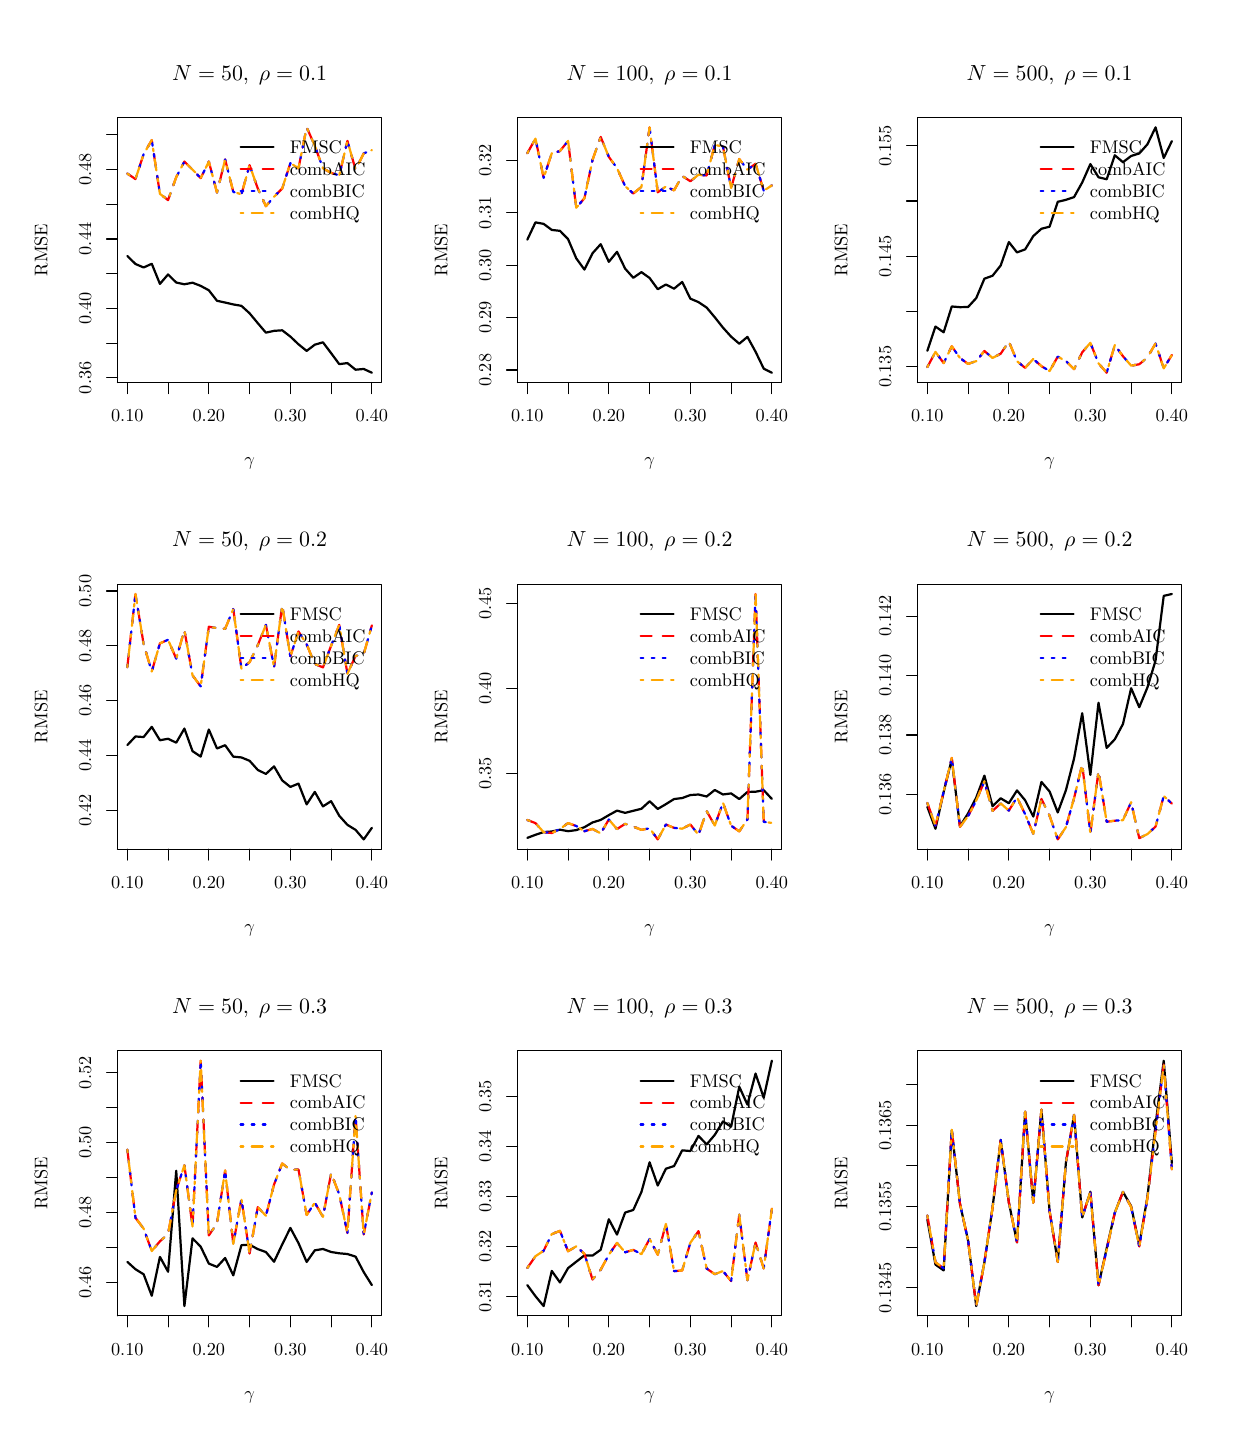
\begin{tikzpicture}[x=1pt,y=1pt]
\definecolor[named]{fillColor}{rgb}{1.00,1.00,1.00}
\path[use as bounding box,fill=fillColor,fill opacity=0.00] (0,0) rectangle (433.62,505.89);
\begin{scope}
\path[clip] ( 32.47,377.65) rectangle (127.91,473.42);
\definecolor[named]{drawColor}{rgb}{0.00,0.00,0.00}

\path[draw=drawColor,line width= 0.8pt,line join=round,line cap=round] ( 36.01,423.38) --
	( 38.95,420.49) --
	( 41.90,419.23) --
	( 44.84,420.56) --
	( 47.79,413.30) --
	( 50.73,416.72) --
	( 53.68,413.79) --
	( 56.63,413.16) --
	( 59.57,413.73) --
	( 62.52,412.58) --
	( 65.46,410.99) --
	( 68.41,407.20) --
	( 71.35,406.56) --
	( 74.30,405.88) --
	( 77.24,405.37) --
	( 80.19,402.67) --
	( 83.14,399.12) --
	( 86.08,395.68) --
	( 89.03,396.33) --
	( 91.97,396.53) --
	( 94.92,394.27) --
	( 97.86,391.47) --
	(100.81,389.09) --
	(103.75,391.33) --
	(106.70,392.19) --
	(109.65,388.27) --
	(112.59,384.30) --
	(115.54,384.69) --
	(118.48,382.29) --
	(121.43,382.56) --
	(124.37,381.20);
\end{scope}
\begin{scope}
\path[clip] (  0.00,  0.00) rectangle (433.62,505.89);
\definecolor[named]{drawColor}{rgb}{0.00,0.00,0.00}

\path[draw=drawColor,line width= 0.4pt,line join=round,line cap=round] ( 36.01,377.65) -- (124.37,377.65);

\path[draw=drawColor,line width= 0.4pt,line join=round,line cap=round] ( 36.01,377.65) -- ( 36.01,373.69);

\path[draw=drawColor,line width= 0.4pt,line join=round,line cap=round] ( 50.73,377.65) -- ( 50.73,373.69);

\path[draw=drawColor,line width= 0.4pt,line join=round,line cap=round] ( 65.46,377.65) -- ( 65.46,373.69);

\path[draw=drawColor,line width= 0.4pt,line join=round,line cap=round] ( 80.19,377.65) -- ( 80.19,373.69);

\path[draw=drawColor,line width= 0.4pt,line join=round,line cap=round] ( 94.92,377.65) -- ( 94.92,373.69);

\path[draw=drawColor,line width= 0.4pt,line join=round,line cap=round] (109.65,377.65) -- (109.65,373.69);

\path[draw=drawColor,line width= 0.4pt,line join=round,line cap=round] (124.37,377.65) -- (124.37,373.69);

\node[text=drawColor,anchor=base,inner sep=0pt, outer sep=0pt, scale=  0.66] at ( 36.01,363.40) {0.10};

\node[text=drawColor,anchor=base,inner sep=0pt, outer sep=0pt, scale=  0.66] at ( 65.46,363.40) {0.20};

\node[text=drawColor,anchor=base,inner sep=0pt, outer sep=0pt, scale=  0.66] at ( 94.92,363.40) {0.30};

\node[text=drawColor,anchor=base,inner sep=0pt, outer sep=0pt, scale=  0.66] at (124.37,363.40) {0.40};

\path[draw=drawColor,line width= 0.4pt,line join=round,line cap=round] ( 32.47,379.34) -- ( 32.47,467.18);

\path[draw=drawColor,line width= 0.4pt,line join=round,line cap=round] ( 32.47,379.34) -- ( 28.51,379.34);

\path[draw=drawColor,line width= 0.4pt,line join=round,line cap=round] ( 32.47,391.89) -- ( 28.51,391.89);

\path[draw=drawColor,line width= 0.4pt,line join=round,line cap=round] ( 32.47,404.44) -- ( 28.51,404.44);

\path[draw=drawColor,line width= 0.4pt,line join=round,line cap=round] ( 32.47,416.99) -- ( 28.51,416.99);

\path[draw=drawColor,line width= 0.4pt,line join=round,line cap=round] ( 32.47,429.54) -- ( 28.51,429.54);

\path[draw=drawColor,line width= 0.4pt,line join=round,line cap=round] ( 32.47,442.08) -- ( 28.51,442.08);

\path[draw=drawColor,line width= 0.4pt,line join=round,line cap=round] ( 32.47,454.63) -- ( 28.51,454.63);

\path[draw=drawColor,line width= 0.4pt,line join=round,line cap=round] ( 32.47,467.18) -- ( 28.51,467.18);

\node[text=drawColor,rotate= 90.00,anchor=base,inner sep=0pt, outer sep=0pt, scale=  0.66] at ( 22.97,379.34) {0.36};

\node[text=drawColor,rotate= 90.00,anchor=base,inner sep=0pt, outer sep=0pt, scale=  0.66] at ( 22.97,404.44) {0.40};

\node[text=drawColor,rotate= 90.00,anchor=base,inner sep=0pt, outer sep=0pt, scale=  0.66] at ( 22.97,429.54) {0.44};

\node[text=drawColor,rotate= 90.00,anchor=base,inner sep=0pt, outer sep=0pt, scale=  0.66] at ( 22.97,454.63) {0.48};

\path[draw=drawColor,line width= 0.4pt,line join=round,line cap=round] ( 32.47,377.65) --
	(127.91,377.65) --
	(127.91,473.42) --
	( 32.47,473.42) --
	( 32.47,377.65);
\end{scope}
\begin{scope}
\path[clip] (  0.00,337.26) rectangle (144.54,505.89);
\definecolor[named]{drawColor}{rgb}{0.00,0.00,0.00}

\node[text=drawColor,anchor=base,inner sep=0pt, outer sep=0pt, scale=  0.79] at ( 80.19,486.92) {\bfseries $N=50, \;\rho=0.1$};

\node[text=drawColor,anchor=base,inner sep=0pt, outer sep=0pt, scale=  0.66] at ( 80.19,347.56) {$\gamma$};

\node[text=drawColor,rotate= 90.00,anchor=base,inner sep=0pt, outer sep=0pt, scale=  0.66] at (  7.13,425.53) {RMSE};
\end{scope}
\begin{scope}
\path[clip] ( 32.47,377.65) rectangle (127.91,473.42);
\definecolor[named]{drawColor}{rgb}{1.00,0.00,0.00}

\path[draw=drawColor,line width= 0.8pt,dash pattern=on 4pt off 4pt ,line join=round,line cap=round] ( 36.01,453.17) --
	( 38.95,451.17) --
	( 41.90,460.17) --
	( 44.84,465.27) --
	( 47.79,445.84) --
	( 50.73,443.57) --
	( 53.68,451.87) --
	( 56.63,457.50) --
	( 59.57,454.60) --
	( 62.52,451.51) --
	( 65.46,457.49) --
	( 68.41,446.28) --
	( 71.35,458.25) --
	( 74.30,446.53) --
	( 77.24,445.68) --
	( 80.19,456.21) --
	( 83.14,447.81) --
	( 86.08,441.36) --
	( 89.03,444.78) --
	( 91.97,447.74) --
	( 94.92,456.93) --
	( 97.86,455.06) --
	(100.81,469.87) --
	(103.75,463.22) --
	(106.70,455.07) --
	(109.65,453.39) --
	(112.59,452.52) --
	(115.54,464.98) --
	(118.48,454.58) --
	(121.43,460.46) --
	(124.37,461.63);
\definecolor[named]{drawColor}{rgb}{0.00,0.00,1.00}

\path[draw=drawColor,line width= 0.8pt,dash pattern=on 1pt off 3pt ,line join=round,line cap=round] ( 36.01,453.17) --
	( 38.95,451.17) --
	( 41.90,460.17) --
	( 44.84,465.27) --
	( 47.79,445.84) --
	( 50.73,443.57) --
	( 53.68,451.87) --
	( 56.63,457.50) --
	( 59.57,454.60) --
	( 62.52,451.51) --
	( 65.46,457.49) --
	( 68.41,446.28) --
	( 71.35,458.25) --
	( 74.30,446.53) --
	( 77.24,445.68) --
	( 80.19,456.21) --
	( 83.14,447.81) --
	( 86.08,441.36) --
	( 89.03,444.78) --
	( 91.97,447.74) --
	( 94.92,456.93) --
	( 97.86,455.06) --
	(100.81,469.87) --
	(103.75,463.22) --
	(106.70,455.07) --
	(109.65,453.39) --
	(112.59,452.52) --
	(115.54,464.98) --
	(118.48,454.58) --
	(121.43,460.46) --
	(124.37,461.63);
\definecolor[named]{drawColor}{rgb}{1.00,0.65,0.00}

\path[draw=drawColor,line width= 0.8pt,dash pattern=on 1pt off 3pt on 4pt off 3pt ,line join=round,line cap=round] ( 36.01,453.17) --
	( 38.95,451.17) --
	( 41.90,460.17) --
	( 44.84,465.27) --
	( 47.79,445.84) --
	( 50.73,443.57) --
	( 53.68,451.87) --
	( 56.63,457.50) --
	( 59.57,454.60) --
	( 62.52,451.51) --
	( 65.46,457.49) --
	( 68.41,446.28) --
	( 71.35,458.25) --
	( 74.30,446.53) --
	( 77.24,445.68) --
	( 80.19,456.21) --
	( 83.14,447.81) --
	( 86.08,441.36) --
	( 89.03,444.78) --
	( 91.97,447.74) --
	( 94.92,456.93) --
	( 97.86,455.06) --
	(100.81,469.87) --
	(103.75,463.22) --
	(106.70,455.07) --
	(109.65,453.39) --
	(112.59,452.52) --
	(115.54,464.98) --
	(118.48,454.58) --
	(121.43,460.46) --
	(124.37,461.63);
\definecolor[named]{drawColor}{rgb}{0.00,0.00,0.00}

\path[draw=drawColor,line width= 0.8pt,line join=round,line cap=round] ( 76.94,462.63) -- ( 88.82,462.63);
\definecolor[named]{drawColor}{rgb}{1.00,0.00,0.00}

\path[draw=drawColor,line width= 0.8pt,dash pattern=on 4pt off 4pt ,line join=round,line cap=round] ( 76.94,454.71) -- ( 88.82,454.71);
\definecolor[named]{drawColor}{rgb}{0.00,0.00,1.00}

\path[draw=drawColor,line width= 0.8pt,dash pattern=on 1pt off 3pt ,line join=round,line cap=round] ( 76.94,446.79) -- ( 88.82,446.79);
\definecolor[named]{drawColor}{rgb}{1.00,0.65,0.00}

\path[draw=drawColor,line width= 0.8pt,dash pattern=on 1pt off 3pt on 4pt off 3pt ,line join=round,line cap=round] ( 76.94,438.87) -- ( 88.82,438.87);
\definecolor[named]{drawColor}{rgb}{0.00,0.00,0.00}

\node[text=drawColor,anchor=base west,inner sep=0pt, outer sep=0pt, scale=  0.66] at ( 94.76,460.35) {FMSC};

\node[text=drawColor,anchor=base west,inner sep=0pt, outer sep=0pt, scale=  0.66] at ( 94.76,452.43) {combAIC};

\node[text=drawColor,anchor=base west,inner sep=0pt, outer sep=0pt, scale=  0.66] at ( 94.76,444.51) {combBIC};

\node[text=drawColor,anchor=base west,inner sep=0pt, outer sep=0pt, scale=  0.66] at ( 94.76,436.59) {combHQ};
\end{scope}
\begin{scope}
\path[clip] (177.01,377.65) rectangle (272.45,473.42);
\definecolor[named]{drawColor}{rgb}{0.00,0.00,0.00}

\path[draw=drawColor,line width= 0.8pt,line join=round,line cap=round] (180.55,429.29) --
	(183.49,435.53) --
	(186.44,434.99) --
	(189.38,432.80) --
	(192.33,432.47) --
	(195.27,429.48) --
	(198.22,422.55) --
	(201.17,418.47) --
	(204.11,424.38) --
	(207.06,427.65) --
	(210.00,421.28) --
	(212.95,424.89) --
	(215.89,418.81) --
	(218.84,415.50) --
	(221.78,417.55) --
	(224.73,415.43) --
	(227.68,411.38) --
	(230.62,413.08) --
	(233.57,411.57) --
	(236.51,414.00) --
	(239.46,407.96) --
	(242.40,406.72) --
	(245.35,404.74) --
	(248.29,401.23) --
	(251.24,397.50) --
	(254.19,394.23) --
	(257.13,391.69) --
	(260.08,394.15) --
	(263.02,388.79) --
	(265.97,382.68) --
	(268.91,381.20);
\end{scope}
\begin{scope}
\path[clip] (  0.00,  0.00) rectangle (433.62,505.89);
\definecolor[named]{drawColor}{rgb}{0.00,0.00,0.00}

\path[draw=drawColor,line width= 0.4pt,line join=round,line cap=round] (180.55,377.65) -- (268.91,377.65);

\path[draw=drawColor,line width= 0.4pt,line join=round,line cap=round] (180.55,377.65) -- (180.55,373.69);

\path[draw=drawColor,line width= 0.4pt,line join=round,line cap=round] (195.27,377.65) -- (195.27,373.69);

\path[draw=drawColor,line width= 0.4pt,line join=round,line cap=round] (210.00,377.65) -- (210.00,373.69);

\path[draw=drawColor,line width= 0.4pt,line join=round,line cap=round] (224.73,377.65) -- (224.73,373.69);

\path[draw=drawColor,line width= 0.4pt,line join=round,line cap=round] (239.46,377.65) -- (239.46,373.69);

\path[draw=drawColor,line width= 0.4pt,line join=round,line cap=round] (254.19,377.65) -- (254.19,373.69);

\path[draw=drawColor,line width= 0.4pt,line join=round,line cap=round] (268.91,377.65) -- (268.91,373.69);

\node[text=drawColor,anchor=base,inner sep=0pt, outer sep=0pt, scale=  0.66] at (180.55,363.40) {0.10};

\node[text=drawColor,anchor=base,inner sep=0pt, outer sep=0pt, scale=  0.66] at (210.00,363.40) {0.20};

\node[text=drawColor,anchor=base,inner sep=0pt, outer sep=0pt, scale=  0.66] at (239.46,363.40) {0.30};

\node[text=drawColor,anchor=base,inner sep=0pt, outer sep=0pt, scale=  0.66] at (268.91,363.40) {0.40};

\path[draw=drawColor,line width= 0.4pt,line join=round,line cap=round] (177.01,382.17) -- (177.01,457.92);

\path[draw=drawColor,line width= 0.4pt,line join=round,line cap=round] (177.01,382.17) -- (173.05,382.17);

\path[draw=drawColor,line width= 0.4pt,line join=round,line cap=round] (177.01,401.11) -- (173.05,401.11);

\path[draw=drawColor,line width= 0.4pt,line join=round,line cap=round] (177.01,420.04) -- (173.05,420.04);

\path[draw=drawColor,line width= 0.4pt,line join=round,line cap=round] (177.01,438.98) -- (173.05,438.98);

\path[draw=drawColor,line width= 0.4pt,line join=round,line cap=round] (177.01,457.92) -- (173.05,457.92);

\node[text=drawColor,rotate= 90.00,anchor=base,inner sep=0pt, outer sep=0pt, scale=  0.66] at (167.51,382.17) {0.28};

\node[text=drawColor,rotate= 90.00,anchor=base,inner sep=0pt, outer sep=0pt, scale=  0.66] at (167.51,401.11) {0.29};

\node[text=drawColor,rotate= 90.00,anchor=base,inner sep=0pt, outer sep=0pt, scale=  0.66] at (167.51,420.04) {0.30};

\node[text=drawColor,rotate= 90.00,anchor=base,inner sep=0pt, outer sep=0pt, scale=  0.66] at (167.51,438.98) {0.31};

\node[text=drawColor,rotate= 90.00,anchor=base,inner sep=0pt, outer sep=0pt, scale=  0.66] at (167.51,457.92) {0.32};

\path[draw=drawColor,line width= 0.4pt,line join=round,line cap=round] (177.01,377.65) --
	(272.45,377.65) --
	(272.45,473.42) --
	(177.01,473.42) --
	(177.01,377.65);
\end{scope}
\begin{scope}
\path[clip] (144.54,337.26) rectangle (289.08,505.89);
\definecolor[named]{drawColor}{rgb}{0.00,0.00,0.00}

\node[text=drawColor,anchor=base,inner sep=0pt, outer sep=0pt, scale=  0.79] at (224.73,486.92) {\bfseries $N=100, \;\rho=0.1$};

\node[text=drawColor,anchor=base,inner sep=0pt, outer sep=0pt, scale=  0.66] at (224.73,347.56) {$\gamma$};

\node[text=drawColor,rotate= 90.00,anchor=base,inner sep=0pt, outer sep=0pt, scale=  0.66] at (151.67,425.53) {RMSE};
\end{scope}
\begin{scope}
\path[clip] (177.01,377.65) rectangle (272.45,473.42);
\definecolor[named]{drawColor}{rgb}{1.00,0.00,0.00}

\path[draw=drawColor,line width= 0.8pt,dash pattern=on 4pt off 4pt ,line join=round,line cap=round] (180.55,460.52) --
	(183.49,465.80) --
	(186.44,451.60) --
	(189.38,460.47) --
	(192.33,461.28) --
	(195.27,464.98) --
	(198.22,440.82) --
	(201.17,444.23) --
	(204.11,458.12) --
	(207.06,466.40) --
	(210.00,459.19) --
	(212.95,455.15) --
	(215.89,448.61) --
	(218.84,445.97) --
	(221.78,448.34) --
	(224.73,469.87) --
	(227.68,446.39) --
	(230.62,448.51) --
	(233.57,447.09) --
	(236.51,452.31) --
	(239.46,450.38) --
	(242.40,452.75) --
	(245.35,452.47) --
	(248.29,463.54) --
	(251.24,462.90) --
	(254.19,447.95) --
	(257.13,458.43) --
	(260.08,454.57) --
	(263.02,456.71) --
	(265.97,446.97) --
	(268.91,448.88);
\definecolor[named]{drawColor}{rgb}{0.00,0.00,1.00}

\path[draw=drawColor,line width= 0.8pt,dash pattern=on 1pt off 3pt ,line join=round,line cap=round] (180.55,460.52) --
	(183.49,465.80) --
	(186.44,451.60) --
	(189.38,460.47) --
	(192.33,461.28) --
	(195.27,464.98) --
	(198.22,440.82) --
	(201.17,444.23) --
	(204.11,458.12) --
	(207.06,466.40) --
	(210.00,459.19) --
	(212.95,455.15) --
	(215.89,448.61) --
	(218.84,445.97) --
	(221.78,448.34) --
	(224.73,469.87) --
	(227.68,446.39) --
	(230.62,448.51) --
	(233.57,447.09) --
	(236.51,452.31) --
	(239.46,450.38) --
	(242.40,452.75) --
	(245.35,452.47) --
	(248.29,463.54) --
	(251.24,462.90) --
	(254.19,447.95) --
	(257.13,458.43) --
	(260.08,454.57) --
	(263.02,456.71) --
	(265.97,446.97) --
	(268.91,448.88);
\definecolor[named]{drawColor}{rgb}{1.00,0.65,0.00}

\path[draw=drawColor,line width= 0.8pt,dash pattern=on 1pt off 3pt on 4pt off 3pt ,line join=round,line cap=round] (180.55,460.52) --
	(183.49,465.80) --
	(186.44,451.60) --
	(189.38,460.47) --
	(192.33,461.28) --
	(195.27,464.98) --
	(198.22,440.82) --
	(201.17,444.23) --
	(204.11,458.12) --
	(207.06,466.40) --
	(210.00,459.19) --
	(212.95,455.15) --
	(215.89,448.61) --
	(218.84,445.97) --
	(221.78,448.34) --
	(224.73,469.87) --
	(227.68,446.39) --
	(230.62,448.51) --
	(233.57,447.09) --
	(236.51,452.31) --
	(239.46,450.38) --
	(242.40,452.75) --
	(245.35,452.47) --
	(248.29,463.54) --
	(251.24,462.90) --
	(254.19,447.95) --
	(257.13,458.43) --
	(260.08,454.57) --
	(263.02,456.71) --
	(265.97,446.97) --
	(268.91,448.88);
\definecolor[named]{drawColor}{rgb}{0.00,0.00,0.00}

\path[draw=drawColor,line width= 0.8pt,line join=round,line cap=round] (221.48,462.63) -- (233.36,462.63);
\definecolor[named]{drawColor}{rgb}{1.00,0.00,0.00}

\path[draw=drawColor,line width= 0.8pt,dash pattern=on 4pt off 4pt ,line join=round,line cap=round] (221.48,454.71) -- (233.36,454.71);
\definecolor[named]{drawColor}{rgb}{0.00,0.00,1.00}

\path[draw=drawColor,line width= 0.8pt,dash pattern=on 1pt off 3pt ,line join=round,line cap=round] (221.48,446.79) -- (233.36,446.79);
\definecolor[named]{drawColor}{rgb}{1.00,0.65,0.00}

\path[draw=drawColor,line width= 0.8pt,dash pattern=on 1pt off 3pt on 4pt off 3pt ,line join=round,line cap=round] (221.48,438.87) -- (233.36,438.87);
\definecolor[named]{drawColor}{rgb}{0.00,0.00,0.00}

\node[text=drawColor,anchor=base west,inner sep=0pt, outer sep=0pt, scale=  0.66] at (239.30,460.35) {FMSC};

\node[text=drawColor,anchor=base west,inner sep=0pt, outer sep=0pt, scale=  0.66] at (239.30,452.43) {combAIC};

\node[text=drawColor,anchor=base west,inner sep=0pt, outer sep=0pt, scale=  0.66] at (239.30,444.51) {combBIC};

\node[text=drawColor,anchor=base west,inner sep=0pt, outer sep=0pt, scale=  0.66] at (239.30,436.59) {combHQ};
\end{scope}
\begin{scope}
\path[clip] (321.55,377.65) rectangle (416.99,473.42);
\definecolor[named]{drawColor}{rgb}{0.00,0.00,0.00}

\path[draw=drawColor,line width= 0.8pt,line join=round,line cap=round] (325.09,389.15) --
	(328.03,397.89) --
	(330.98,395.81) --
	(333.92,405.14) --
	(336.87,404.89) --
	(339.81,404.94) --
	(342.76,408.17) --
	(345.71,415.18) --
	(348.65,416.24) --
	(351.60,419.96) --
	(354.54,428.42) --
	(357.49,424.68) --
	(360.43,425.77) --
	(363.38,430.58) --
	(366.32,433.22) --
	(369.27,433.98) --
	(372.22,442.96) --
	(375.16,443.67) --
	(378.11,444.67) --
	(381.05,449.95) --
	(384.00,456.60) --
	(386.94,451.83) --
	(389.89,451.11) --
	(392.83,459.77) --
	(395.78,457.28) --
	(398.73,459.52) --
	(401.67,460.43) --
	(404.62,463.74) --
	(407.56,469.87) --
	(410.51,458.80) --
	(413.45,464.89);
\end{scope}
\begin{scope}
\path[clip] (  0.00,  0.00) rectangle (433.62,505.89);
\definecolor[named]{drawColor}{rgb}{0.00,0.00,0.00}

\path[draw=drawColor,line width= 0.4pt,line join=round,line cap=round] (325.09,377.65) -- (413.45,377.65);

\path[draw=drawColor,line width= 0.4pt,line join=round,line cap=round] (325.09,377.65) -- (325.09,373.69);

\path[draw=drawColor,line width= 0.4pt,line join=round,line cap=round] (339.81,377.65) -- (339.81,373.69);

\path[draw=drawColor,line width= 0.4pt,line join=round,line cap=round] (354.54,377.65) -- (354.54,373.69);

\path[draw=drawColor,line width= 0.4pt,line join=round,line cap=round] (369.27,377.65) -- (369.27,373.69);

\path[draw=drawColor,line width= 0.4pt,line join=round,line cap=round] (384.00,377.65) -- (384.00,373.69);

\path[draw=drawColor,line width= 0.4pt,line join=round,line cap=round] (398.73,377.65) -- (398.73,373.69);

\path[draw=drawColor,line width= 0.4pt,line join=round,line cap=round] (413.45,377.65) -- (413.45,373.69);

\node[text=drawColor,anchor=base,inner sep=0pt, outer sep=0pt, scale=  0.66] at (325.09,363.40) {0.10};

\node[text=drawColor,anchor=base,inner sep=0pt, outer sep=0pt, scale=  0.66] at (354.54,363.40) {0.20};

\node[text=drawColor,anchor=base,inner sep=0pt, outer sep=0pt, scale=  0.66] at (384.00,363.40) {0.30};

\node[text=drawColor,anchor=base,inner sep=0pt, outer sep=0pt, scale=  0.66] at (413.45,363.40) {0.40};

\path[draw=drawColor,line width= 0.4pt,line join=round,line cap=round] (321.55,383.40) -- (321.55,463.20);

\path[draw=drawColor,line width= 0.4pt,line join=round,line cap=round] (321.55,383.40) -- (317.59,383.40);

\path[draw=drawColor,line width= 0.4pt,line join=round,line cap=round] (321.55,403.35) -- (317.59,403.35);

\path[draw=drawColor,line width= 0.4pt,line join=round,line cap=round] (321.55,423.30) -- (317.59,423.30);

\path[draw=drawColor,line width= 0.4pt,line join=round,line cap=round] (321.55,443.25) -- (317.59,443.25);

\path[draw=drawColor,line width= 0.4pt,line join=round,line cap=round] (321.55,463.20) -- (317.59,463.20);

\node[text=drawColor,rotate= 90.00,anchor=base,inner sep=0pt, outer sep=0pt, scale=  0.66] at (312.05,383.40) {0.135};

\node[text=drawColor,rotate= 90.00,anchor=base,inner sep=0pt, outer sep=0pt, scale=  0.66] at (312.05,423.30) {0.145};

\node[text=drawColor,rotate= 90.00,anchor=base,inner sep=0pt, outer sep=0pt, scale=  0.66] at (312.05,463.20) {0.155};

\path[draw=drawColor,line width= 0.4pt,line join=round,line cap=round] (321.55,377.65) --
	(416.99,377.65) --
	(416.99,473.42) --
	(321.55,473.42) --
	(321.55,377.65);
\end{scope}
\begin{scope}
\path[clip] (289.08,337.26) rectangle (433.62,505.89);
\definecolor[named]{drawColor}{rgb}{0.00,0.00,0.00}

\node[text=drawColor,anchor=base,inner sep=0pt, outer sep=0pt, scale=  0.79] at (369.27,486.92) {\bfseries $N=500, \;\rho=0.1$};

\node[text=drawColor,anchor=base,inner sep=0pt, outer sep=0pt, scale=  0.66] at (369.27,347.56) {$\gamma$};

\node[text=drawColor,rotate= 90.00,anchor=base,inner sep=0pt, outer sep=0pt, scale=  0.66] at (296.21,425.53) {RMSE};
\end{scope}
\begin{scope}
\path[clip] (321.55,377.65) rectangle (416.99,473.42);
\definecolor[named]{drawColor}{rgb}{1.00,0.00,0.00}

\path[draw=drawColor,line width= 0.8pt,dash pattern=on 4pt off 4pt ,line join=round,line cap=round] (325.09,383.23) --
	(328.03,388.73) --
	(330.98,384.68) --
	(333.92,390.75) --
	(336.87,386.53) --
	(339.81,384.38) --
	(342.76,385.40) --
	(345.71,389.05) --
	(348.65,386.53) --
	(351.60,388.08) --
	(354.54,392.48) --
	(357.49,385.37) --
	(360.43,382.95) --
	(363.38,386.17) --
	(366.32,383.56) --
	(369.27,381.82) --
	(372.22,387.02) --
	(375.16,385.41) --
	(378.11,382.49) --
	(381.05,388.57) --
	(384.00,392.00) --
	(386.94,384.61) --
	(389.89,381.20) --
	(392.83,391.18) --
	(395.78,387.16) --
	(398.73,383.77) --
	(401.67,384.25) --
	(404.62,386.74) --
	(407.56,391.77) --
	(410.51,382.78) --
	(413.45,387.62);
\definecolor[named]{drawColor}{rgb}{0.00,0.00,1.00}

\path[draw=drawColor,line width= 0.8pt,dash pattern=on 1pt off 3pt ,line join=round,line cap=round] (325.09,383.23) --
	(328.03,388.73) --
	(330.98,384.68) --
	(333.92,390.75) --
	(336.87,386.53) --
	(339.81,384.38) --
	(342.76,385.40) --
	(345.71,389.05) --
	(348.65,386.53) --
	(351.60,388.08) --
	(354.54,392.48) --
	(357.49,385.37) --
	(360.43,382.95) --
	(363.38,386.17) --
	(366.32,383.56) --
	(369.27,381.82) --
	(372.22,387.02) --
	(375.16,385.41) --
	(378.11,382.49) --
	(381.05,388.57) --
	(384.00,392.00) --
	(386.94,384.61) --
	(389.89,381.20) --
	(392.83,391.18) --
	(395.78,387.16) --
	(398.73,383.77) --
	(401.67,384.25) --
	(404.62,386.74) --
	(407.56,391.77) --
	(410.51,382.78) --
	(413.45,387.62);
\definecolor[named]{drawColor}{rgb}{1.00,0.65,0.00}

\path[draw=drawColor,line width= 0.8pt,dash pattern=on 1pt off 3pt on 4pt off 3pt ,line join=round,line cap=round] (325.09,383.23) --
	(328.03,388.73) --
	(330.98,384.68) --
	(333.92,390.75) --
	(336.87,386.53) --
	(339.81,384.38) --
	(342.76,385.40) --
	(345.71,389.05) --
	(348.65,386.53) --
	(351.60,388.08) --
	(354.54,392.48) --
	(357.49,385.37) --
	(360.43,382.95) --
	(363.38,386.17) --
	(366.32,383.56) --
	(369.27,381.82) --
	(372.22,387.02) --
	(375.16,385.41) --
	(378.11,382.49) --
	(381.05,388.57) --
	(384.00,392.00) --
	(386.94,384.61) --
	(389.89,381.20) --
	(392.83,391.18) --
	(395.78,387.16) --
	(398.73,383.77) --
	(401.67,384.25) --
	(404.62,386.74) --
	(407.56,391.77) --
	(410.51,382.78) --
	(413.45,387.62);
\definecolor[named]{drawColor}{rgb}{0.00,0.00,0.00}

\path[draw=drawColor,line width= 0.8pt,line join=round,line cap=round] (366.02,462.63) -- (377.90,462.63);
\definecolor[named]{drawColor}{rgb}{1.00,0.00,0.00}

\path[draw=drawColor,line width= 0.8pt,dash pattern=on 4pt off 4pt ,line join=round,line cap=round] (366.02,454.71) -- (377.90,454.71);
\definecolor[named]{drawColor}{rgb}{0.00,0.00,1.00}

\path[draw=drawColor,line width= 0.8pt,dash pattern=on 1pt off 3pt ,line join=round,line cap=round] (366.02,446.79) -- (377.90,446.79);
\definecolor[named]{drawColor}{rgb}{1.00,0.65,0.00}

\path[draw=drawColor,line width= 0.8pt,dash pattern=on 1pt off 3pt on 4pt off 3pt ,line join=round,line cap=round] (366.02,438.87) -- (377.90,438.87);
\definecolor[named]{drawColor}{rgb}{0.00,0.00,0.00}

\node[text=drawColor,anchor=base west,inner sep=0pt, outer sep=0pt, scale=  0.66] at (383.84,460.35) {FMSC};

\node[text=drawColor,anchor=base west,inner sep=0pt, outer sep=0pt, scale=  0.66] at (383.84,452.43) {combAIC};

\node[text=drawColor,anchor=base west,inner sep=0pt, outer sep=0pt, scale=  0.66] at (383.84,444.51) {combBIC};

\node[text=drawColor,anchor=base west,inner sep=0pt, outer sep=0pt, scale=  0.66] at (383.84,436.59) {combHQ};
\end{scope}
\begin{scope}
\path[clip] ( 32.47,209.02) rectangle (127.91,304.79);
\definecolor[named]{drawColor}{rgb}{0.00,0.00,0.00}

\path[draw=drawColor,line width= 0.8pt,line join=round,line cap=round] ( 36.01,246.65) --
	( 38.95,249.76) --
	( 41.90,249.55) --
	( 44.84,253.24) --
	( 47.79,248.40) --
	( 50.73,248.93) --
	( 53.68,247.52) --
	( 56.63,252.61) --
	( 59.57,244.46) --
	( 62.52,242.50) --
	( 65.46,252.27) --
	( 68.41,245.42) --
	( 71.35,246.60) --
	( 74.30,242.48) --
	( 77.24,242.18) --
	( 80.19,240.97) --
	( 83.14,237.68) --
	( 86.08,236.22) --
	( 89.03,238.96) --
	( 91.97,233.89) --
	( 94.92,231.53) --
	( 97.86,232.73) --
	(100.81,225.22) --
	(103.75,229.73) --
	(106.70,224.50) --
	(109.65,226.38) --
	(112.59,221.10) --
	(115.54,217.82) --
	(118.48,216.02) --
	(121.43,212.57) --
	(124.37,216.74);
\end{scope}
\begin{scope}
\path[clip] (  0.00,  0.00) rectangle (433.62,505.89);
\definecolor[named]{drawColor}{rgb}{0.00,0.00,0.00}

\path[draw=drawColor,line width= 0.4pt,line join=round,line cap=round] ( 36.01,209.02) -- (124.37,209.02);

\path[draw=drawColor,line width= 0.4pt,line join=round,line cap=round] ( 36.01,209.02) -- ( 36.01,205.06);

\path[draw=drawColor,line width= 0.4pt,line join=round,line cap=round] ( 50.73,209.02) -- ( 50.73,205.06);

\path[draw=drawColor,line width= 0.4pt,line join=round,line cap=round] ( 65.46,209.02) -- ( 65.46,205.06);

\path[draw=drawColor,line width= 0.4pt,line join=round,line cap=round] ( 80.19,209.02) -- ( 80.19,205.06);

\path[draw=drawColor,line width= 0.4pt,line join=round,line cap=round] ( 94.92,209.02) -- ( 94.92,205.06);

\path[draw=drawColor,line width= 0.4pt,line join=round,line cap=round] (109.65,209.02) -- (109.65,205.06);

\path[draw=drawColor,line width= 0.4pt,line join=round,line cap=round] (124.37,209.02) -- (124.37,205.06);

\node[text=drawColor,anchor=base,inner sep=0pt, outer sep=0pt, scale=  0.66] at ( 36.01,194.77) {0.10};

\node[text=drawColor,anchor=base,inner sep=0pt, outer sep=0pt, scale=  0.66] at ( 65.46,194.77) {0.20};

\node[text=drawColor,anchor=base,inner sep=0pt, outer sep=0pt, scale=  0.66] at ( 94.92,194.77) {0.30};

\node[text=drawColor,anchor=base,inner sep=0pt, outer sep=0pt, scale=  0.66] at (124.37,194.77) {0.40};

\path[draw=drawColor,line width= 0.4pt,line join=round,line cap=round] ( 32.47,223.06) -- ( 32.47,302.31);

\path[draw=drawColor,line width= 0.4pt,line join=round,line cap=round] ( 32.47,223.06) -- ( 28.51,223.06);

\path[draw=drawColor,line width= 0.4pt,line join=round,line cap=round] ( 32.47,242.87) -- ( 28.51,242.87);

\path[draw=drawColor,line width= 0.4pt,line join=round,line cap=round] ( 32.47,262.68) -- ( 28.51,262.68);

\path[draw=drawColor,line width= 0.4pt,line join=round,line cap=round] ( 32.47,282.49) -- ( 28.51,282.49);

\path[draw=drawColor,line width= 0.4pt,line join=round,line cap=round] ( 32.47,302.31) -- ( 28.51,302.31);

\node[text=drawColor,rotate= 90.00,anchor=base,inner sep=0pt, outer sep=0pt, scale=  0.66] at ( 22.97,223.06) {0.42};

\node[text=drawColor,rotate= 90.00,anchor=base,inner sep=0pt, outer sep=0pt, scale=  0.66] at ( 22.97,242.87) {0.44};

\node[text=drawColor,rotate= 90.00,anchor=base,inner sep=0pt, outer sep=0pt, scale=  0.66] at ( 22.97,262.68) {0.46};

\node[text=drawColor,rotate= 90.00,anchor=base,inner sep=0pt, outer sep=0pt, scale=  0.66] at ( 22.97,282.49) {0.48};

\node[text=drawColor,rotate= 90.00,anchor=base,inner sep=0pt, outer sep=0pt, scale=  0.66] at ( 22.97,302.31) {0.50};

\path[draw=drawColor,line width= 0.4pt,line join=round,line cap=round] ( 32.47,209.02) --
	(127.91,209.02) --
	(127.91,304.79) --
	( 32.47,304.79) --
	( 32.47,209.02);
\end{scope}
\begin{scope}
\path[clip] (  0.00,168.63) rectangle (144.54,337.26);
\definecolor[named]{drawColor}{rgb}{0.00,0.00,0.00}

\node[text=drawColor,anchor=base,inner sep=0pt, outer sep=0pt, scale=  0.79] at ( 80.19,318.29) {\bfseries $N=50, \;\rho=0.2$};

\node[text=drawColor,anchor=base,inner sep=0pt, outer sep=0pt, scale=  0.66] at ( 80.19,178.93) {$\gamma$};

\node[text=drawColor,rotate= 90.00,anchor=base,inner sep=0pt, outer sep=0pt, scale=  0.66] at (  7.13,256.90) {RMSE};
\end{scope}
\begin{scope}
\path[clip] ( 32.47,209.02) rectangle (127.91,304.79);
\definecolor[named]{drawColor}{rgb}{1.00,0.00,0.00}

\path[draw=drawColor,line width= 0.8pt,dash pattern=on 4pt off 4pt ,line join=round,line cap=round] ( 36.01,274.80) --
	( 38.95,301.24) --
	( 41.90,283.11) --
	( 44.84,273.23) --
	( 47.79,283.41) --
	( 50.73,284.71) --
	( 53.68,277.87) --
	( 56.63,288.17) --
	( 59.57,271.86) --
	( 62.52,267.85) --
	( 65.46,289.41) --
	( 68.41,288.94) --
	( 71.35,288.66) --
	( 74.30,295.80) --
	( 77.24,274.30) --
	( 80.19,276.62) --
	( 83.14,282.73) --
	( 86.08,290.09) --
	( 89.03,274.92) --
	( 91.97,297.20) --
	( 94.92,278.71) --
	( 97.86,287.71) --
	(100.81,283.03) --
	(103.75,275.98) --
	(106.70,274.72) --
	(109.65,282.55) --
	(112.59,290.08) --
	(115.54,272.42) --
	(118.48,278.88) --
	(121.43,279.53) --
	(124.37,289.90);
\definecolor[named]{drawColor}{rgb}{0.00,0.00,1.00}

\path[draw=drawColor,line width= 0.8pt,dash pattern=on 1pt off 3pt ,line join=round,line cap=round] ( 36.01,274.80) --
	( 38.95,301.24) --
	( 41.90,283.11) --
	( 44.84,273.23) --
	( 47.79,283.41) --
	( 50.73,284.71) --
	( 53.68,277.87) --
	( 56.63,288.17) --
	( 59.57,271.86) --
	( 62.52,267.85) --
	( 65.46,289.41) --
	( 68.41,288.94) --
	( 71.35,288.66) --
	( 74.30,295.80) --
	( 77.24,274.30) --
	( 80.19,276.62) --
	( 83.14,282.73) --
	( 86.08,290.09) --
	( 89.03,274.92) --
	( 91.97,297.20) --
	( 94.92,278.71) --
	( 97.86,287.71) --
	(100.81,283.03) --
	(103.75,275.98) --
	(106.70,274.72) --
	(109.65,282.55) --
	(112.59,290.08) --
	(115.54,272.42) --
	(118.48,278.88) --
	(121.43,279.53) --
	(124.37,289.90);
\definecolor[named]{drawColor}{rgb}{1.00,0.65,0.00}

\path[draw=drawColor,line width= 0.8pt,dash pattern=on 1pt off 3pt on 4pt off 3pt ,line join=round,line cap=round] ( 36.01,274.80) --
	( 38.95,301.24) --
	( 41.90,283.11) --
	( 44.84,273.23) --
	( 47.79,283.41) --
	( 50.73,284.71) --
	( 53.68,277.87) --
	( 56.63,288.17) --
	( 59.57,271.86) --
	( 62.52,267.85) --
	( 65.46,289.41) --
	( 68.41,288.94) --
	( 71.35,288.66) --
	( 74.30,295.80) --
	( 77.24,274.30) --
	( 80.19,276.62) --
	( 83.14,282.73) --
	( 86.08,290.09) --
	( 89.03,274.92) --
	( 91.97,297.20) --
	( 94.92,278.71) --
	( 97.86,287.71) --
	(100.81,283.03) --
	(103.75,275.98) --
	(106.70,274.72) --
	(109.65,282.55) --
	(112.59,290.08) --
	(115.54,272.42) --
	(118.48,278.88) --
	(121.43,279.53) --
	(124.37,289.90);
\definecolor[named]{drawColor}{rgb}{0.00,0.00,0.00}

\path[draw=drawColor,line width= 0.8pt,line join=round,line cap=round] ( 76.94,294.00) -- ( 88.82,294.00);
\definecolor[named]{drawColor}{rgb}{1.00,0.00,0.00}

\path[draw=drawColor,line width= 0.8pt,dash pattern=on 4pt off 4pt ,line join=round,line cap=round] ( 76.94,286.08) -- ( 88.82,286.08);
\definecolor[named]{drawColor}{rgb}{0.00,0.00,1.00}

\path[draw=drawColor,line width= 0.8pt,dash pattern=on 1pt off 3pt ,line join=round,line cap=round] ( 76.94,278.16) -- ( 88.82,278.16);
\definecolor[named]{drawColor}{rgb}{1.00,0.65,0.00}

\path[draw=drawColor,line width= 0.8pt,dash pattern=on 1pt off 3pt on 4pt off 3pt ,line join=round,line cap=round] ( 76.94,270.24) -- ( 88.82,270.24);
\definecolor[named]{drawColor}{rgb}{0.00,0.00,0.00}

\node[text=drawColor,anchor=base west,inner sep=0pt, outer sep=0pt, scale=  0.66] at ( 94.76,291.72) {FMSC};

\node[text=drawColor,anchor=base west,inner sep=0pt, outer sep=0pt, scale=  0.66] at ( 94.76,283.80) {combAIC};

\node[text=drawColor,anchor=base west,inner sep=0pt, outer sep=0pt, scale=  0.66] at ( 94.76,275.88) {combBIC};

\node[text=drawColor,anchor=base west,inner sep=0pt, outer sep=0pt, scale=  0.66] at ( 94.76,267.96) {combHQ};
\end{scope}
\begin{scope}
\path[clip] (177.01,209.02) rectangle (272.45,304.79);
\definecolor[named]{drawColor}{rgb}{0.00,0.00,0.00}

\path[draw=drawColor,line width= 0.8pt,line join=round,line cap=round] (180.55,213.12) --
	(183.49,214.23) --
	(186.44,215.23) --
	(189.38,215.42) --
	(192.33,216.08) --
	(195.27,215.54) --
	(198.22,215.92) --
	(201.17,216.98) --
	(204.11,218.69) --
	(207.06,219.61) --
	(210.00,221.34) --
	(212.95,222.97) --
	(215.89,222.16) --
	(218.84,222.90) --
	(221.78,223.64) --
	(224.73,226.34) --
	(227.68,223.58) --
	(230.62,225.31) --
	(233.57,227.15) --
	(236.51,227.51) --
	(239.46,228.60) --
	(242.40,228.79) --
	(245.35,228.07) --
	(248.29,230.43) --
	(251.24,228.80) --
	(254.19,229.19) --
	(257.13,227.14) --
	(260.08,229.71) --
	(263.02,229.80) --
	(265.97,230.34) --
	(268.91,227.19);
\end{scope}
\begin{scope}
\path[clip] (  0.00,  0.00) rectangle (433.62,505.89);
\definecolor[named]{drawColor}{rgb}{0.00,0.00,0.00}

\path[draw=drawColor,line width= 0.4pt,line join=round,line cap=round] (180.55,209.02) -- (268.91,209.02);

\path[draw=drawColor,line width= 0.4pt,line join=round,line cap=round] (180.55,209.02) -- (180.55,205.06);

\path[draw=drawColor,line width= 0.4pt,line join=round,line cap=round] (195.27,209.02) -- (195.27,205.06);

\path[draw=drawColor,line width= 0.4pt,line join=round,line cap=round] (210.00,209.02) -- (210.00,205.06);

\path[draw=drawColor,line width= 0.4pt,line join=round,line cap=round] (224.73,209.02) -- (224.73,205.06);

\path[draw=drawColor,line width= 0.4pt,line join=round,line cap=round] (239.46,209.02) -- (239.46,205.06);

\path[draw=drawColor,line width= 0.4pt,line join=round,line cap=round] (254.19,209.02) -- (254.19,205.06);

\path[draw=drawColor,line width= 0.4pt,line join=round,line cap=round] (268.91,209.02) -- (268.91,205.06);

\node[text=drawColor,anchor=base,inner sep=0pt, outer sep=0pt, scale=  0.66] at (180.55,194.77) {0.10};

\node[text=drawColor,anchor=base,inner sep=0pt, outer sep=0pt, scale=  0.66] at (210.00,194.77) {0.20};

\node[text=drawColor,anchor=base,inner sep=0pt, outer sep=0pt, scale=  0.66] at (239.46,194.77) {0.30};

\node[text=drawColor,anchor=base,inner sep=0pt, outer sep=0pt, scale=  0.66] at (268.91,194.77) {0.40};

\path[draw=drawColor,line width= 0.4pt,line join=round,line cap=round] (177.01,236.38) -- (177.01,297.75);

\path[draw=drawColor,line width= 0.4pt,line join=round,line cap=round] (177.01,236.38) -- (173.05,236.38);

\path[draw=drawColor,line width= 0.4pt,line join=round,line cap=round] (177.01,267.07) -- (173.05,267.07);

\path[draw=drawColor,line width= 0.4pt,line join=round,line cap=round] (177.01,297.75) -- (173.05,297.75);

\node[text=drawColor,rotate= 90.00,anchor=base,inner sep=0pt, outer sep=0pt, scale=  0.66] at (167.51,236.38) {0.35};

\node[text=drawColor,rotate= 90.00,anchor=base,inner sep=0pt, outer sep=0pt, scale=  0.66] at (167.51,267.07) {0.40};

\node[text=drawColor,rotate= 90.00,anchor=base,inner sep=0pt, outer sep=0pt, scale=  0.66] at (167.51,297.75) {0.45};

\path[draw=drawColor,line width= 0.4pt,line join=round,line cap=round] (177.01,209.02) --
	(272.45,209.02) --
	(272.45,304.79) --
	(177.01,304.79) --
	(177.01,209.02);
\end{scope}
\begin{scope}
\path[clip] (144.54,168.63) rectangle (289.08,337.26);
\definecolor[named]{drawColor}{rgb}{0.00,0.00,0.00}

\node[text=drawColor,anchor=base,inner sep=0pt, outer sep=0pt, scale=  0.79] at (224.73,318.29) {\bfseries $N=100, \;\rho=0.2$};

\node[text=drawColor,anchor=base,inner sep=0pt, outer sep=0pt, scale=  0.66] at (224.73,178.93) {$\gamma$};

\node[text=drawColor,rotate= 90.00,anchor=base,inner sep=0pt, outer sep=0pt, scale=  0.66] at (151.67,256.90) {RMSE};
\end{scope}
\begin{scope}
\path[clip] (177.01,209.02) rectangle (272.45,304.79);
\definecolor[named]{drawColor}{rgb}{1.00,0.00,0.00}

\path[draw=drawColor,line width= 0.8pt,dash pattern=on 4pt off 4pt ,line join=round,line cap=round] (180.55,219.60) --
	(183.49,218.45) --
	(186.44,215.18) --
	(189.38,214.88) --
	(192.33,216.33) --
	(195.27,218.46) --
	(198.22,217.42) --
	(201.17,215.52) --
	(204.11,216.34) --
	(207.06,214.74) --
	(210.00,219.75) --
	(212.95,216.30) --
	(215.89,218.20) --
	(218.84,217.19) --
	(221.78,216.02) --
	(224.73,216.59) --
	(227.68,212.57) --
	(230.62,217.94) --
	(233.57,216.74) --
	(236.51,216.44) --
	(239.46,217.95) --
	(242.40,214.23) --
	(245.35,222.79) --
	(248.29,217.56) --
	(251.24,225.83) --
	(254.19,217.52) --
	(257.13,215.48) --
	(260.08,219.78) --
	(263.02,301.24) --
	(265.97,218.92) --
	(268.91,218.52);
\definecolor[named]{drawColor}{rgb}{0.00,0.00,1.00}

\path[draw=drawColor,line width= 0.8pt,dash pattern=on 1pt off 3pt ,line join=round,line cap=round] (180.55,219.60) --
	(183.49,218.45) --
	(186.44,215.18) --
	(189.38,214.88) --
	(192.33,216.33) --
	(195.27,218.46) --
	(198.22,217.42) --
	(201.17,215.52) --
	(204.11,216.34) --
	(207.06,214.74) --
	(210.00,219.75) --
	(212.95,216.30) --
	(215.89,218.20) --
	(218.84,217.19) --
	(221.78,216.02) --
	(224.73,216.59) --
	(227.68,212.57) --
	(230.62,217.94) --
	(233.57,216.74) --
	(236.51,216.44) --
	(239.46,217.95) --
	(242.40,214.23) --
	(245.35,222.79) --
	(248.29,217.56) --
	(251.24,225.83) --
	(254.19,217.52) --
	(257.13,215.48) --
	(260.08,219.78) --
	(263.02,301.24) --
	(265.97,218.92) --
	(268.91,218.52);
\definecolor[named]{drawColor}{rgb}{1.00,0.65,0.00}

\path[draw=drawColor,line width= 0.8pt,dash pattern=on 1pt off 3pt on 4pt off 3pt ,line join=round,line cap=round] (180.55,219.60) --
	(183.49,218.45) --
	(186.44,215.18) --
	(189.38,214.88) --
	(192.33,216.33) --
	(195.27,218.46) --
	(198.22,217.42) --
	(201.17,215.52) --
	(204.11,216.34) --
	(207.06,214.74) --
	(210.00,219.75) --
	(212.95,216.30) --
	(215.89,218.20) --
	(218.84,217.19) --
	(221.78,216.02) --
	(224.73,216.59) --
	(227.68,212.57) --
	(230.62,217.94) --
	(233.57,216.74) --
	(236.51,216.44) --
	(239.46,217.95) --
	(242.40,214.23) --
	(245.35,222.79) --
	(248.29,217.56) --
	(251.24,225.83) --
	(254.19,217.52) --
	(257.13,215.48) --
	(260.08,219.78) --
	(263.02,301.24) --
	(265.97,218.92) --
	(268.91,218.52);
\definecolor[named]{drawColor}{rgb}{0.00,0.00,0.00}

\path[draw=drawColor,line width= 0.8pt,line join=round,line cap=round] (221.48,294.00) -- (233.36,294.00);
\definecolor[named]{drawColor}{rgb}{1.00,0.00,0.00}

\path[draw=drawColor,line width= 0.8pt,dash pattern=on 4pt off 4pt ,line join=round,line cap=round] (221.48,286.08) -- (233.36,286.08);
\definecolor[named]{drawColor}{rgb}{0.00,0.00,1.00}

\path[draw=drawColor,line width= 0.8pt,dash pattern=on 1pt off 3pt ,line join=round,line cap=round] (221.48,278.16) -- (233.36,278.16);
\definecolor[named]{drawColor}{rgb}{1.00,0.65,0.00}

\path[draw=drawColor,line width= 0.8pt,dash pattern=on 1pt off 3pt on 4pt off 3pt ,line join=round,line cap=round] (221.48,270.24) -- (233.36,270.24);
\definecolor[named]{drawColor}{rgb}{0.00,0.00,0.00}

\node[text=drawColor,anchor=base west,inner sep=0pt, outer sep=0pt, scale=  0.66] at (239.30,291.72) {FMSC};

\node[text=drawColor,anchor=base west,inner sep=0pt, outer sep=0pt, scale=  0.66] at (239.30,283.80) {combAIC};

\node[text=drawColor,anchor=base west,inner sep=0pt, outer sep=0pt, scale=  0.66] at (239.30,275.88) {combBIC};

\node[text=drawColor,anchor=base west,inner sep=0pt, outer sep=0pt, scale=  0.66] at (239.30,267.96) {combHQ};
\end{scope}
\begin{scope}
\path[clip] (321.55,209.02) rectangle (416.99,304.79);
\definecolor[named]{drawColor}{rgb}{0.00,0.00,0.00}

\path[draw=drawColor,line width= 0.8pt,line join=round,line cap=round] (325.09,224.33) --
	(328.03,216.41) --
	(330.98,229.69) --
	(333.92,241.53) --
	(336.87,217.32) --
	(339.81,221.94) --
	(342.76,227.69) --
	(345.71,235.61) --
	(348.65,224.57) --
	(351.60,227.42) --
	(354.54,225.65) --
	(357.49,230.26) --
	(360.43,226.70) --
	(363.38,220.80) --
	(366.32,233.33) --
	(369.27,229.87) --
	(372.22,222.32) --
	(375.16,230.31) --
	(378.11,241.79) --
	(381.05,258.18) --
	(384.00,235.85) --
	(386.94,261.96) --
	(389.89,245.63) --
	(392.83,248.74) --
	(395.78,254.27) --
	(398.73,267.21) --
	(401.67,260.34) --
	(404.62,267.47) --
	(407.56,277.22) --
	(410.51,300.57) --
	(413.45,301.24);
\end{scope}
\begin{scope}
\path[clip] (  0.00,  0.00) rectangle (433.62,505.89);
\definecolor[named]{drawColor}{rgb}{0.00,0.00,0.00}

\path[draw=drawColor,line width= 0.4pt,line join=round,line cap=round] (325.09,209.02) -- (413.45,209.02);

\path[draw=drawColor,line width= 0.4pt,line join=round,line cap=round] (325.09,209.02) -- (325.09,205.06);

\path[draw=drawColor,line width= 0.4pt,line join=round,line cap=round] (339.81,209.02) -- (339.81,205.06);

\path[draw=drawColor,line width= 0.4pt,line join=round,line cap=round] (354.54,209.02) -- (354.54,205.06);

\path[draw=drawColor,line width= 0.4pt,line join=round,line cap=round] (369.27,209.02) -- (369.27,205.06);

\path[draw=drawColor,line width= 0.4pt,line join=round,line cap=round] (384.00,209.02) -- (384.00,205.06);

\path[draw=drawColor,line width= 0.4pt,line join=round,line cap=round] (398.73,209.02) -- (398.73,205.06);

\path[draw=drawColor,line width= 0.4pt,line join=round,line cap=round] (413.45,209.02) -- (413.45,205.06);

\node[text=drawColor,anchor=base,inner sep=0pt, outer sep=0pt, scale=  0.66] at (325.09,194.77) {0.10};

\node[text=drawColor,anchor=base,inner sep=0pt, outer sep=0pt, scale=  0.66] at (354.54,194.77) {0.20};

\node[text=drawColor,anchor=base,inner sep=0pt, outer sep=0pt, scale=  0.66] at (384.00,194.77) {0.30};

\node[text=drawColor,anchor=base,inner sep=0pt, outer sep=0pt, scale=  0.66] at (413.45,194.77) {0.40};

\path[draw=drawColor,line width= 0.4pt,line join=round,line cap=round] (321.55,228.80) -- (321.55,293.27);

\path[draw=drawColor,line width= 0.4pt,line join=round,line cap=round] (321.55,228.80) -- (317.59,228.80);

\path[draw=drawColor,line width= 0.4pt,line join=round,line cap=round] (321.55,250.29) -- (317.59,250.29);

\path[draw=drawColor,line width= 0.4pt,line join=round,line cap=round] (321.55,271.78) -- (317.59,271.78);

\path[draw=drawColor,line width= 0.4pt,line join=round,line cap=round] (321.55,293.27) -- (317.59,293.27);

\node[text=drawColor,rotate= 90.00,anchor=base,inner sep=0pt, outer sep=0pt, scale=  0.66] at (312.05,228.80) {0.136};

\node[text=drawColor,rotate= 90.00,anchor=base,inner sep=0pt, outer sep=0pt, scale=  0.66] at (312.05,250.29) {0.138};

\node[text=drawColor,rotate= 90.00,anchor=base,inner sep=0pt, outer sep=0pt, scale=  0.66] at (312.05,271.78) {0.140};

\node[text=drawColor,rotate= 90.00,anchor=base,inner sep=0pt, outer sep=0pt, scale=  0.66] at (312.05,293.27) {0.142};

\path[draw=drawColor,line width= 0.4pt,line join=round,line cap=round] (321.55,209.02) --
	(416.99,209.02) --
	(416.99,304.79) --
	(321.55,304.79) --
	(321.55,209.02);
\end{scope}
\begin{scope}
\path[clip] (289.08,168.63) rectangle (433.62,337.26);
\definecolor[named]{drawColor}{rgb}{0.00,0.00,0.00}

\node[text=drawColor,anchor=base,inner sep=0pt, outer sep=0pt, scale=  0.79] at (369.27,318.29) {\bfseries $N=500, \;\rho=0.2$};

\node[text=drawColor,anchor=base,inner sep=0pt, outer sep=0pt, scale=  0.66] at (369.27,178.93) {$\gamma$};

\node[text=drawColor,rotate= 90.00,anchor=base,inner sep=0pt, outer sep=0pt, scale=  0.66] at (296.21,256.90) {RMSE};
\end{scope}
\begin{scope}
\path[clip] (321.55,209.02) rectangle (416.99,304.79);
\definecolor[named]{drawColor}{rgb}{1.00,0.00,0.00}

\path[draw=drawColor,line width= 0.8pt,dash pattern=on 4pt off 4pt ,line join=round,line cap=round] (325.09,225.74) --
	(328.03,217.54) --
	(330.98,229.75) --
	(333.92,242.01) --
	(336.87,217.11) --
	(339.81,220.98) --
	(342.76,226.63) --
	(345.71,233.54) --
	(348.65,222.86) --
	(351.60,225.59) --
	(354.54,222.97) --
	(357.49,227.77) --
	(360.43,221.65) --
	(363.38,214.56) --
	(366.32,227.18) --
	(369.27,221.11) --
	(372.22,212.57) --
	(375.16,216.99) --
	(378.11,227.47) --
	(381.05,239.71) --
	(384.00,214.80) --
	(386.94,237.23) --
	(389.89,218.93) --
	(392.83,219.33) --
	(395.78,219.52) --
	(398.73,226.02) --
	(401.67,213.01) --
	(404.62,214.47) --
	(407.56,217.19) --
	(410.51,228.24) --
	(413.45,225.51);
\definecolor[named]{drawColor}{rgb}{0.00,0.00,1.00}

\path[draw=drawColor,line width= 0.8pt,dash pattern=on 1pt off 3pt ,line join=round,line cap=round] (325.09,225.74) --
	(328.03,217.54) --
	(330.98,229.75) --
	(333.92,242.01) --
	(336.87,217.11) --
	(339.81,220.98) --
	(342.76,226.63) --
	(345.71,233.54) --
	(348.65,222.86) --
	(351.60,225.59) --
	(354.54,222.97) --
	(357.49,227.77) --
	(360.43,221.65) --
	(363.38,214.56) --
	(366.32,227.18) --
	(369.27,221.11) --
	(372.22,212.57) --
	(375.16,216.99) --
	(378.11,227.47) --
	(381.05,239.71) --
	(384.00,214.80) --
	(386.94,237.23) --
	(389.89,218.93) --
	(392.83,219.33) --
	(395.78,219.52) --
	(398.73,226.02) --
	(401.67,213.01) --
	(404.62,214.47) --
	(407.56,217.19) --
	(410.51,228.24) --
	(413.45,225.51);
\definecolor[named]{drawColor}{rgb}{1.00,0.65,0.00}

\path[draw=drawColor,line width= 0.8pt,dash pattern=on 1pt off 3pt on 4pt off 3pt ,line join=round,line cap=round] (325.09,225.74) --
	(328.03,217.54) --
	(330.98,229.75) --
	(333.92,242.01) --
	(336.87,217.11) --
	(339.81,220.98) --
	(342.76,226.63) --
	(345.71,233.54) --
	(348.65,222.86) --
	(351.60,225.59) --
	(354.54,222.97) --
	(357.49,227.77) --
	(360.43,221.65) --
	(363.38,214.56) --
	(366.32,227.18) --
	(369.27,221.11) --
	(372.22,212.57) --
	(375.16,216.99) --
	(378.11,227.47) --
	(381.05,239.71) --
	(384.00,214.80) --
	(386.94,237.23) --
	(389.89,218.93) --
	(392.83,219.33) --
	(395.78,219.52) --
	(398.73,226.02) --
	(401.67,213.01) --
	(404.62,214.47) --
	(407.56,217.19) --
	(410.51,228.24) --
	(413.45,225.51);
\definecolor[named]{drawColor}{rgb}{0.00,0.00,0.00}

\path[draw=drawColor,line width= 0.8pt,line join=round,line cap=round] (366.02,294.00) -- (377.90,294.00);
\definecolor[named]{drawColor}{rgb}{1.00,0.00,0.00}

\path[draw=drawColor,line width= 0.8pt,dash pattern=on 4pt off 4pt ,line join=round,line cap=round] (366.02,286.08) -- (377.90,286.08);
\definecolor[named]{drawColor}{rgb}{0.00,0.00,1.00}

\path[draw=drawColor,line width= 0.8pt,dash pattern=on 1pt off 3pt ,line join=round,line cap=round] (366.02,278.16) -- (377.90,278.16);
\definecolor[named]{drawColor}{rgb}{1.00,0.65,0.00}

\path[draw=drawColor,line width= 0.8pt,dash pattern=on 1pt off 3pt on 4pt off 3pt ,line join=round,line cap=round] (366.02,270.24) -- (377.90,270.24);
\definecolor[named]{drawColor}{rgb}{0.00,0.00,0.00}

\node[text=drawColor,anchor=base west,inner sep=0pt, outer sep=0pt, scale=  0.66] at (383.84,291.72) {FMSC};

\node[text=drawColor,anchor=base west,inner sep=0pt, outer sep=0pt, scale=  0.66] at (383.84,283.80) {combAIC};

\node[text=drawColor,anchor=base west,inner sep=0pt, outer sep=0pt, scale=  0.66] at (383.84,275.88) {combBIC};

\node[text=drawColor,anchor=base west,inner sep=0pt, outer sep=0pt, scale=  0.66] at (383.84,267.96) {combHQ};
\end{scope}
\begin{scope}
\path[clip] ( 32.47, 40.39) rectangle (127.91,136.16);
\definecolor[named]{drawColor}{rgb}{0.00,0.00,0.00}

\path[draw=drawColor,line width= 0.8pt,line join=round,line cap=round] ( 36.01, 59.92) --
	( 38.95, 57.25) --
	( 41.90, 55.43) --
	( 44.84, 47.67) --
	( 47.79, 61.72) --
	( 50.73, 56.36) --
	( 53.68, 92.86) --
	( 56.63, 43.94) --
	( 59.57, 68.42) --
	( 62.52, 65.39) --
	( 65.46, 59.29) --
	( 68.41, 58.09) --
	( 71.35, 61.31) --
	( 74.30, 55.03) --
	( 77.24, 65.94) --
	( 80.19, 66.12) --
	( 83.14, 64.52) --
	( 86.08, 63.47) --
	( 89.03, 59.96) --
	( 91.97, 66.20) --
	( 94.92, 72.17) --
	( 97.86, 66.69) --
	(100.81, 59.88) --
	(103.75, 64.07) --
	(106.70, 64.57) --
	(109.65, 63.48) --
	(112.59, 63.01) --
	(115.54, 62.75) --
	(118.48, 61.81) --
	(121.43, 56.21) --
	(124.37, 51.52);
\end{scope}
\begin{scope}
\path[clip] (  0.00,  0.00) rectangle (433.62,505.89);
\definecolor[named]{drawColor}{rgb}{0.00,0.00,0.00}

\path[draw=drawColor,line width= 0.4pt,line join=round,line cap=round] ( 36.01, 40.39) -- (124.37, 40.39);

\path[draw=drawColor,line width= 0.4pt,line join=round,line cap=round] ( 36.01, 40.39) -- ( 36.01, 36.43);

\path[draw=drawColor,line width= 0.4pt,line join=round,line cap=round] ( 50.73, 40.39) -- ( 50.73, 36.43);

\path[draw=drawColor,line width= 0.4pt,line join=round,line cap=round] ( 65.46, 40.39) -- ( 65.46, 36.43);

\path[draw=drawColor,line width= 0.4pt,line join=round,line cap=round] ( 80.19, 40.39) -- ( 80.19, 36.43);

\path[draw=drawColor,line width= 0.4pt,line join=round,line cap=round] ( 94.92, 40.39) -- ( 94.92, 36.43);

\path[draw=drawColor,line width= 0.4pt,line join=round,line cap=round] (109.65, 40.39) -- (109.65, 36.43);

\path[draw=drawColor,line width= 0.4pt,line join=round,line cap=round] (124.37, 40.39) -- (124.37, 36.43);

\node[text=drawColor,anchor=base,inner sep=0pt, outer sep=0pt, scale=  0.66] at ( 36.01, 26.14) {0.10};

\node[text=drawColor,anchor=base,inner sep=0pt, outer sep=0pt, scale=  0.66] at ( 65.46, 26.14) {0.20};

\node[text=drawColor,anchor=base,inner sep=0pt, outer sep=0pt, scale=  0.66] at ( 94.92, 26.14) {0.30};

\node[text=drawColor,anchor=base,inner sep=0pt, outer sep=0pt, scale=  0.66] at (124.37, 26.14) {0.40};

\path[draw=drawColor,line width= 0.4pt,line join=round,line cap=round] ( 32.47, 52.51) -- ( 32.47,128.20);

\path[draw=drawColor,line width= 0.4pt,line join=round,line cap=round] ( 32.47, 52.51) -- ( 28.51, 52.51);

\path[draw=drawColor,line width= 0.4pt,line join=round,line cap=round] ( 32.47, 65.13) -- ( 28.51, 65.13);

\path[draw=drawColor,line width= 0.4pt,line join=round,line cap=round] ( 32.47, 77.74) -- ( 28.51, 77.74);

\path[draw=drawColor,line width= 0.4pt,line join=round,line cap=round] ( 32.47, 90.36) -- ( 28.51, 90.36);

\path[draw=drawColor,line width= 0.4pt,line join=round,line cap=round] ( 32.47,102.97) -- ( 28.51,102.97);

\path[draw=drawColor,line width= 0.4pt,line join=round,line cap=round] ( 32.47,115.58) -- ( 28.51,115.58);

\path[draw=drawColor,line width= 0.4pt,line join=round,line cap=round] ( 32.47,128.20) -- ( 28.51,128.20);

\node[text=drawColor,rotate= 90.00,anchor=base,inner sep=0pt, outer sep=0pt, scale=  0.66] at ( 22.97, 52.51) {0.46};

\node[text=drawColor,rotate= 90.00,anchor=base,inner sep=0pt, outer sep=0pt, scale=  0.66] at ( 22.97, 77.74) {0.48};

\node[text=drawColor,rotate= 90.00,anchor=base,inner sep=0pt, outer sep=0pt, scale=  0.66] at ( 22.97,102.97) {0.50};

\node[text=drawColor,rotate= 90.00,anchor=base,inner sep=0pt, outer sep=0pt, scale=  0.66] at ( 22.97,128.20) {0.52};

\path[draw=drawColor,line width= 0.4pt,line join=round,line cap=round] ( 32.47, 40.39) --
	(127.91, 40.39) --
	(127.91,136.16) --
	( 32.47,136.16) --
	( 32.47, 40.39);
\end{scope}
\begin{scope}
\path[clip] (  0.00,  0.00) rectangle (144.54,168.63);
\definecolor[named]{drawColor}{rgb}{0.00,0.00,0.00}

\node[text=drawColor,anchor=base,inner sep=0pt, outer sep=0pt, scale=  0.79] at ( 80.19,149.66) {\bfseries $N=50, \;\rho=0.3$};

\node[text=drawColor,anchor=base,inner sep=0pt, outer sep=0pt, scale=  0.66] at ( 80.19, 10.30) {$\gamma$};

\node[text=drawColor,rotate= 90.00,anchor=base,inner sep=0pt, outer sep=0pt, scale=  0.66] at (  7.13, 88.28) {RMSE};
\end{scope}
\begin{scope}
\path[clip] ( 32.47, 40.39) rectangle (127.91,136.16);
\definecolor[named]{drawColor}{rgb}{1.00,0.00,0.00}

\path[draw=drawColor,line width= 0.8pt,dash pattern=on 4pt off 4pt ,line join=round,line cap=round] ( 36.01,100.46) --
	( 38.95, 75.84) --
	( 41.90, 71.92) --
	( 44.84, 63.83) --
	( 47.79, 67.34) --
	( 50.73, 70.00) --
	( 53.68, 85.81) --
	( 56.63, 94.81) --
	( 59.57, 72.70) --
	( 62.52,132.61) --
	( 65.46, 69.48) --
	( 68.41, 73.81) --
	( 71.35, 92.93) --
	( 74.30, 66.41) --
	( 77.24, 82.66) --
	( 80.19, 62.90) --
	( 83.14, 79.68) --
	( 86.08, 76.60) --
	( 89.03, 87.87) --
	( 91.97, 95.47) --
	( 94.92, 93.14) --
	( 97.86, 93.30) --
	(100.81, 76.87) --
	(103.75, 81.30) --
	(106.70, 76.15) --
	(109.65, 91.94) --
	(112.59, 84.32) --
	(115.54, 70.33) --
	(118.48,112.60) --
	(121.43, 69.80) --
	(124.37, 85.02);
\definecolor[named]{drawColor}{rgb}{0.00,0.00,1.00}

\path[draw=drawColor,line width= 0.8pt,dash pattern=on 1pt off 3pt ,line join=round,line cap=round] ( 36.01,100.46) --
	( 38.95, 75.84) --
	( 41.90, 71.92) --
	( 44.84, 63.83) --
	( 47.79, 67.34) --
	( 50.73, 70.00) --
	( 53.68, 85.81) --
	( 56.63, 94.81) --
	( 59.57, 72.70) --
	( 62.52,132.61) --
	( 65.46, 69.48) --
	( 68.41, 73.81) --
	( 71.35, 92.93) --
	( 74.30, 66.41) --
	( 77.24, 82.66) --
	( 80.19, 62.90) --
	( 83.14, 79.68) --
	( 86.08, 76.60) --
	( 89.03, 87.87) --
	( 91.97, 95.47) --
	( 94.92, 93.14) --
	( 97.86, 93.30) --
	(100.81, 76.87) --
	(103.75, 81.30) --
	(106.70, 76.15) --
	(109.65, 91.94) --
	(112.59, 84.32) --
	(115.54, 70.33) --
	(118.48,112.60) --
	(121.43, 69.80) --
	(124.37, 85.02);
\definecolor[named]{drawColor}{rgb}{1.00,0.65,0.00}

\path[draw=drawColor,line width= 0.8pt,dash pattern=on 1pt off 3pt on 4pt off 3pt ,line join=round,line cap=round] ( 36.01,100.46) --
	( 38.95, 75.84) --
	( 41.90, 71.92) --
	( 44.84, 63.83) --
	( 47.79, 67.34) --
	( 50.73, 70.00) --
	( 53.68, 85.81) --
	( 56.63, 94.81) --
	( 59.57, 72.70) --
	( 62.52,132.61) --
	( 65.46, 69.48) --
	( 68.41, 73.81) --
	( 71.35, 92.93) --
	( 74.30, 66.41) --
	( 77.24, 82.66) --
	( 80.19, 62.90) --
	( 83.14, 79.68) --
	( 86.08, 76.60) --
	( 89.03, 87.87) --
	( 91.97, 95.47) --
	( 94.92, 93.14) --
	( 97.86, 93.30) --
	(100.81, 76.87) --
	(103.75, 81.30) --
	(106.70, 76.15) --
	(109.65, 91.94) --
	(112.59, 84.32) --
	(115.54, 70.33) --
	(118.48,112.60) --
	(121.43, 69.80) --
	(124.37, 85.02);
\definecolor[named]{drawColor}{rgb}{0.00,0.00,0.00}

\path[draw=drawColor,line width= 0.8pt,line join=round,line cap=round] ( 76.94,125.37) -- ( 88.82,125.37);
\definecolor[named]{drawColor}{rgb}{1.00,0.00,0.00}

\path[draw=drawColor,line width= 0.8pt,dash pattern=on 4pt off 4pt ,line join=round,line cap=round] ( 76.94,117.45) -- ( 88.82,117.45);
\definecolor[named]{drawColor}{rgb}{0.00,0.00,1.00}

\path[draw=drawColor,line width= 0.8pt,dash pattern=on 1pt off 3pt ,line join=round,line cap=round] ( 76.94,109.53) -- ( 88.82,109.53);
\definecolor[named]{drawColor}{rgb}{1.00,0.65,0.00}

\path[draw=drawColor,line width= 0.8pt,dash pattern=on 1pt off 3pt on 4pt off 3pt ,line join=round,line cap=round] ( 76.94,101.61) -- ( 88.82,101.61);
\definecolor[named]{drawColor}{rgb}{0.00,0.00,0.00}

\node[text=drawColor,anchor=base west,inner sep=0pt, outer sep=0pt, scale=  0.66] at ( 94.76,123.09) {FMSC};

\node[text=drawColor,anchor=base west,inner sep=0pt, outer sep=0pt, scale=  0.66] at ( 94.76,115.17) {combAIC};

\node[text=drawColor,anchor=base west,inner sep=0pt, outer sep=0pt, scale=  0.66] at ( 94.76,107.25) {combBIC};

\node[text=drawColor,anchor=base west,inner sep=0pt, outer sep=0pt, scale=  0.66] at ( 94.76, 99.33) {combHQ};
\end{scope}
\begin{scope}
\path[clip] (177.01, 40.39) rectangle (272.45,136.16);
\definecolor[named]{drawColor}{rgb}{0.00,0.00,0.00}

\path[draw=drawColor,line width= 0.8pt,line join=round,line cap=round] (180.55, 51.51) --
	(183.49, 47.51) --
	(186.44, 43.94) --
	(189.38, 56.63) --
	(192.33, 52.49) --
	(195.27, 57.65) --
	(198.22, 59.96) --
	(201.17, 62.25) --
	(204.11, 62.18) --
	(207.06, 64.29) --
	(210.00, 75.30) --
	(212.95, 69.77) --
	(215.89, 77.73) --
	(218.84, 78.67) --
	(221.78, 85.17) --
	(224.73, 95.89) --
	(227.68, 87.50) --
	(230.62, 93.57) --
	(233.57, 94.53) --
	(236.51,100.21) --
	(239.46, 99.96) --
	(242.40,105.42) --
	(245.35,102.35) --
	(248.29,105.82) --
	(251.24,110.65) --
	(254.19,108.76) --
	(257.13,123.20) --
	(260.08,116.74) --
	(263.02,127.95) --
	(265.97,119.23) --
	(268.91,132.61);
\end{scope}
\begin{scope}
\path[clip] (  0.00,  0.00) rectangle (433.62,505.89);
\definecolor[named]{drawColor}{rgb}{0.00,0.00,0.00}

\path[draw=drawColor,line width= 0.4pt,line join=round,line cap=round] (180.55, 40.39) -- (268.91, 40.39);

\path[draw=drawColor,line width= 0.4pt,line join=round,line cap=round] (180.55, 40.39) -- (180.55, 36.43);

\path[draw=drawColor,line width= 0.4pt,line join=round,line cap=round] (195.27, 40.39) -- (195.27, 36.43);

\path[draw=drawColor,line width= 0.4pt,line join=round,line cap=round] (210.00, 40.39) -- (210.00, 36.43);

\path[draw=drawColor,line width= 0.4pt,line join=round,line cap=round] (224.73, 40.39) -- (224.73, 36.43);

\path[draw=drawColor,line width= 0.4pt,line join=round,line cap=round] (239.46, 40.39) -- (239.46, 36.43);

\path[draw=drawColor,line width= 0.4pt,line join=round,line cap=round] (254.19, 40.39) -- (254.19, 36.43);

\path[draw=drawColor,line width= 0.4pt,line join=round,line cap=round] (268.91, 40.39) -- (268.91, 36.43);

\node[text=drawColor,anchor=base,inner sep=0pt, outer sep=0pt, scale=  0.66] at (180.55, 26.14) {0.10};

\node[text=drawColor,anchor=base,inner sep=0pt, outer sep=0pt, scale=  0.66] at (210.00, 26.14) {0.20};

\node[text=drawColor,anchor=base,inner sep=0pt, outer sep=0pt, scale=  0.66] at (239.46, 26.14) {0.30};

\node[text=drawColor,anchor=base,inner sep=0pt, outer sep=0pt, scale=  0.66] at (268.91, 26.14) {0.40};

\path[draw=drawColor,line width= 0.4pt,line join=round,line cap=round] (177.01, 47.34) -- (177.01,119.63);

\path[draw=drawColor,line width= 0.4pt,line join=round,line cap=round] (177.01, 47.34) -- (173.05, 47.34);

\path[draw=drawColor,line width= 0.4pt,line join=round,line cap=round] (177.01, 65.41) -- (173.05, 65.41);

\path[draw=drawColor,line width= 0.4pt,line join=round,line cap=round] (177.01, 83.49) -- (173.05, 83.49);

\path[draw=drawColor,line width= 0.4pt,line join=round,line cap=round] (177.01,101.56) -- (173.05,101.56);

\path[draw=drawColor,line width= 0.4pt,line join=round,line cap=round] (177.01,119.63) -- (173.05,119.63);

\node[text=drawColor,rotate= 90.00,anchor=base,inner sep=0pt, outer sep=0pt, scale=  0.66] at (167.51, 47.34) {0.31};

\node[text=drawColor,rotate= 90.00,anchor=base,inner sep=0pt, outer sep=0pt, scale=  0.66] at (167.51, 65.41) {0.32};

\node[text=drawColor,rotate= 90.00,anchor=base,inner sep=0pt, outer sep=0pt, scale=  0.66] at (167.51, 83.49) {0.33};

\node[text=drawColor,rotate= 90.00,anchor=base,inner sep=0pt, outer sep=0pt, scale=  0.66] at (167.51,101.56) {0.34};

\node[text=drawColor,rotate= 90.00,anchor=base,inner sep=0pt, outer sep=0pt, scale=  0.66] at (167.51,119.63) {0.35};

\path[draw=drawColor,line width= 0.4pt,line join=round,line cap=round] (177.01, 40.39) --
	(272.45, 40.39) --
	(272.45,136.16) --
	(177.01,136.16) --
	(177.01, 40.39);
\end{scope}
\begin{scope}
\path[clip] (144.54,  0.00) rectangle (289.08,168.63);
\definecolor[named]{drawColor}{rgb}{0.00,0.00,0.00}

\node[text=drawColor,anchor=base,inner sep=0pt, outer sep=0pt, scale=  0.79] at (224.73,149.66) {\bfseries $N=100, \;\rho=0.3$};

\node[text=drawColor,anchor=base,inner sep=0pt, outer sep=0pt, scale=  0.66] at (224.73, 10.30) {$\gamma$};

\node[text=drawColor,rotate= 90.00,anchor=base,inner sep=0pt, outer sep=0pt, scale=  0.66] at (151.67, 88.27) {RMSE};
\end{scope}
\begin{scope}
\path[clip] (177.01, 40.39) rectangle (272.45,136.16);
\definecolor[named]{drawColor}{rgb}{1.00,0.00,0.00}

\path[draw=drawColor,line width= 0.8pt,dash pattern=on 4pt off 4pt ,line join=round,line cap=round] (180.55, 57.71) --
	(183.49, 61.95) --
	(186.44, 63.93) --
	(189.38, 69.93) --
	(192.33, 71.13) --
	(195.27, 63.75) --
	(198.22, 65.52) --
	(201.17, 62.81) --
	(204.11, 53.52) --
	(207.06, 57.09) --
	(210.00, 62.48) --
	(212.95, 66.76) --
	(215.89, 63.37) --
	(218.84, 64.25) --
	(221.78, 62.68) --
	(224.73, 68.19) --
	(227.68, 62.49) --
	(230.62, 73.64) --
	(233.57, 56.55) --
	(236.51, 56.81) --
	(239.46, 66.82) --
	(242.40, 71.02) --
	(245.35, 57.49) --
	(248.29, 55.46) --
	(251.24, 56.60) --
	(254.19, 52.96) --
	(257.13, 77.01) --
	(260.08, 53.24) --
	(263.02, 66.91) --
	(265.97, 57.52) --
	(268.91, 79.10);
\definecolor[named]{drawColor}{rgb}{0.00,0.00,1.00}

\path[draw=drawColor,line width= 0.8pt,dash pattern=on 1pt off 3pt ,line join=round,line cap=round] (180.55, 57.71) --
	(183.49, 61.95) --
	(186.44, 63.93) --
	(189.38, 69.93) --
	(192.33, 71.13) --
	(195.27, 63.75) --
	(198.22, 65.52) --
	(201.17, 62.81) --
	(204.11, 53.52) --
	(207.06, 57.09) --
	(210.00, 62.48) --
	(212.95, 66.76) --
	(215.89, 63.37) --
	(218.84, 64.25) --
	(221.78, 62.68) --
	(224.73, 68.19) --
	(227.68, 62.49) --
	(230.62, 73.64) --
	(233.57, 56.55) --
	(236.51, 56.81) --
	(239.46, 66.82) --
	(242.40, 71.02) --
	(245.35, 57.49) --
	(248.29, 55.46) --
	(251.24, 56.60) --
	(254.19, 52.96) --
	(257.13, 77.01) --
	(260.08, 53.24) --
	(263.02, 66.91) --
	(265.97, 57.52) --
	(268.91, 79.10);
\definecolor[named]{drawColor}{rgb}{1.00,0.65,0.00}

\path[draw=drawColor,line width= 0.8pt,dash pattern=on 1pt off 3pt on 4pt off 3pt ,line join=round,line cap=round] (180.55, 57.71) --
	(183.49, 61.95) --
	(186.44, 63.93) --
	(189.38, 69.93) --
	(192.33, 71.13) --
	(195.27, 63.75) --
	(198.22, 65.52) --
	(201.17, 62.81) --
	(204.11, 53.52) --
	(207.06, 57.09) --
	(210.00, 62.48) --
	(212.95, 66.76) --
	(215.89, 63.37) --
	(218.84, 64.25) --
	(221.78, 62.68) --
	(224.73, 68.19) --
	(227.68, 62.49) --
	(230.62, 73.64) --
	(233.57, 56.55) --
	(236.51, 56.81) --
	(239.46, 66.82) --
	(242.40, 71.02) --
	(245.35, 57.49) --
	(248.29, 55.46) --
	(251.24, 56.60) --
	(254.19, 52.96) --
	(257.13, 77.01) --
	(260.08, 53.24) --
	(263.02, 66.91) --
	(265.97, 57.52) --
	(268.91, 79.10);
\definecolor[named]{drawColor}{rgb}{0.00,0.00,0.00}

\path[draw=drawColor,line width= 0.8pt,line join=round,line cap=round] (221.48,125.37) -- (233.36,125.37);
\definecolor[named]{drawColor}{rgb}{1.00,0.00,0.00}

\path[draw=drawColor,line width= 0.8pt,dash pattern=on 4pt off 4pt ,line join=round,line cap=round] (221.48,117.45) -- (233.36,117.45);
\definecolor[named]{drawColor}{rgb}{0.00,0.00,1.00}

\path[draw=drawColor,line width= 0.8pt,dash pattern=on 1pt off 3pt ,line join=round,line cap=round] (221.48,109.53) -- (233.36,109.53);
\definecolor[named]{drawColor}{rgb}{1.00,0.65,0.00}

\path[draw=drawColor,line width= 0.8pt,dash pattern=on 1pt off 3pt on 4pt off 3pt ,line join=round,line cap=round] (221.48,101.61) -- (233.36,101.61);
\definecolor[named]{drawColor}{rgb}{0.00,0.00,0.00}

\node[text=drawColor,anchor=base west,inner sep=0pt, outer sep=0pt, scale=  0.66] at (239.30,123.09) {FMSC};

\node[text=drawColor,anchor=base west,inner sep=0pt, outer sep=0pt, scale=  0.66] at (239.30,115.17) {combAIC};

\node[text=drawColor,anchor=base west,inner sep=0pt, outer sep=0pt, scale=  0.66] at (239.30,107.25) {combBIC};

\node[text=drawColor,anchor=base west,inner sep=0pt, outer sep=0pt, scale=  0.66] at (239.30, 99.33) {combHQ};
\end{scope}
\begin{scope}
\path[clip] (321.55, 40.39) rectangle (416.99,136.16);
\definecolor[named]{drawColor}{rgb}{0.00,0.00,0.00}

\path[draw=drawColor,line width= 0.8pt,line join=round,line cap=round] (325.09, 75.17) --
	(328.03, 58.92) --
	(330.98, 56.83) --
	(333.92,107.47) --
	(336.87, 80.94) --
	(339.81, 67.62) --
	(342.76, 43.94) --
	(345.71, 59.73) --
	(348.65, 79.47) --
	(351.60,103.99) --
	(354.54, 81.42) --
	(357.49, 66.95) --
	(360.43,114.19) --
	(363.38, 81.29) --
	(366.32,114.94) --
	(369.27, 78.20) --
	(372.22, 59.89) --
	(375.16, 95.74) --
	(378.11,113.02) --
	(381.05, 75.96) --
	(384.00, 85.25) --
	(386.94, 51.45) --
	(389.89, 64.79) --
	(392.83, 77.67) --
	(395.78, 85.20) --
	(398.73, 80.05) --
	(401.67, 65.98) --
	(404.62, 83.43) --
	(407.56,109.55) --
	(410.51,132.61) --
	(413.45, 95.55);
\end{scope}
\begin{scope}
\path[clip] (  0.00,  0.00) rectangle (433.62,505.89);
\definecolor[named]{drawColor}{rgb}{0.00,0.00,0.00}

\path[draw=drawColor,line width= 0.4pt,line join=round,line cap=round] (325.09, 40.39) -- (413.45, 40.39);

\path[draw=drawColor,line width= 0.4pt,line join=round,line cap=round] (325.09, 40.39) -- (325.09, 36.43);

\path[draw=drawColor,line width= 0.4pt,line join=round,line cap=round] (339.81, 40.39) -- (339.81, 36.43);

\path[draw=drawColor,line width= 0.4pt,line join=round,line cap=round] (354.54, 40.39) -- (354.54, 36.43);

\path[draw=drawColor,line width= 0.4pt,line join=round,line cap=round] (369.27, 40.39) -- (369.27, 36.43);

\path[draw=drawColor,line width= 0.4pt,line join=round,line cap=round] (384.00, 40.39) -- (384.00, 36.43);

\path[draw=drawColor,line width= 0.4pt,line join=round,line cap=round] (398.73, 40.39) -- (398.73, 36.43);

\path[draw=drawColor,line width= 0.4pt,line join=round,line cap=round] (413.45, 40.39) -- (413.45, 36.43);

\node[text=drawColor,anchor=base,inner sep=0pt, outer sep=0pt, scale=  0.66] at (325.09, 26.14) {0.10};

\node[text=drawColor,anchor=base,inner sep=0pt, outer sep=0pt, scale=  0.66] at (354.54, 26.14) {0.20};

\node[text=drawColor,anchor=base,inner sep=0pt, outer sep=0pt, scale=  0.66] at (384.00, 26.14) {0.30};

\node[text=drawColor,anchor=base,inner sep=0pt, outer sep=0pt, scale=  0.66] at (413.45, 26.14) {0.40};

\path[draw=drawColor,line width= 0.4pt,line join=round,line cap=round] (321.55, 50.59) -- (321.55,123.94);

\path[draw=drawColor,line width= 0.4pt,line join=round,line cap=round] (321.55, 50.59) -- (317.59, 50.59);

\path[draw=drawColor,line width= 0.4pt,line join=round,line cap=round] (321.55, 65.26) -- (317.59, 65.26);

\path[draw=drawColor,line width= 0.4pt,line join=round,line cap=round] (321.55, 79.93) -- (317.59, 79.93);

\path[draw=drawColor,line width= 0.4pt,line join=round,line cap=round] (321.55, 94.60) -- (317.59, 94.60);

\path[draw=drawColor,line width= 0.4pt,line join=round,line cap=round] (321.55,109.27) -- (317.59,109.27);

\path[draw=drawColor,line width= 0.4pt,line join=round,line cap=round] (321.55,123.94) -- (317.59,123.94);

\node[text=drawColor,rotate= 90.00,anchor=base,inner sep=0pt, outer sep=0pt, scale=  0.66] at (312.05, 50.59) {0.1345};

\node[text=drawColor,rotate= 90.00,anchor=base,inner sep=0pt, outer sep=0pt, scale=  0.66] at (312.05, 79.93) {0.1355};

\node[text=drawColor,rotate= 90.00,anchor=base,inner sep=0pt, outer sep=0pt, scale=  0.66] at (312.05,109.27) {0.1365};

\path[draw=drawColor,line width= 0.4pt,line join=round,line cap=round] (321.55, 40.39) --
	(416.99, 40.39) --
	(416.99,136.16) --
	(321.55,136.16) --
	(321.55, 40.39);
\end{scope}
\begin{scope}
\path[clip] (289.08,  0.00) rectangle (433.62,168.63);
\definecolor[named]{drawColor}{rgb}{0.00,0.00,0.00}

\node[text=drawColor,anchor=base,inner sep=0pt, outer sep=0pt, scale=  0.79] at (369.27,149.66) {\bfseries $N=500, \;\rho=0.3$};

\node[text=drawColor,anchor=base,inner sep=0pt, outer sep=0pt, scale=  0.66] at (369.27, 10.30) {$\gamma$};

\node[text=drawColor,rotate= 90.00,anchor=base,inner sep=0pt, outer sep=0pt, scale=  0.66] at (296.21, 88.27) {RMSE};
\end{scope}
\begin{scope}
\path[clip] (321.55, 40.39) rectangle (416.99,136.16);
\definecolor[named]{drawColor}{rgb}{1.00,0.00,0.00}

\path[draw=drawColor,line width= 0.8pt,dash pattern=on 4pt off 4pt ,line join=round,line cap=round] (325.09, 76.68) --
	(328.03, 59.78) --
	(330.98, 57.55) --
	(333.92,107.68) --
	(336.87, 80.97) --
	(339.81, 67.71) --
	(342.76, 43.95) --
	(345.71, 59.73) --
	(348.65, 79.47) --
	(351.60,103.99) --
	(354.54, 81.42) --
	(357.49, 66.95) --
	(360.43,114.19) --
	(363.38, 81.29) --
	(366.32,114.94) --
	(369.27, 78.20) --
	(372.22, 59.89) --
	(375.16, 95.74) --
	(378.11,113.02) --
	(381.05, 75.96) --
	(384.00, 85.25) --
	(386.94, 51.45) --
	(389.89, 64.24) --
	(392.83, 77.67) --
	(395.78, 85.20) --
	(398.73, 79.71) --
	(401.67, 65.46) --
	(404.62, 82.97) --
	(407.56,107.14) --
	(410.51,131.22) --
	(413.45, 93.34);
\definecolor[named]{drawColor}{rgb}{0.00,0.00,1.00}

\path[draw=drawColor,line width= 0.8pt,dash pattern=on 1pt off 3pt ,line join=round,line cap=round] (325.09, 76.68) --
	(328.03, 59.78) --
	(330.98, 57.55) --
	(333.92,107.68) --
	(336.87, 80.97) --
	(339.81, 67.71) --
	(342.76, 43.95) --
	(345.71, 59.73) --
	(348.65, 79.47) --
	(351.60,103.99) --
	(354.54, 81.42) --
	(357.49, 66.95) --
	(360.43,114.19) --
	(363.38, 81.29) --
	(366.32,114.94) --
	(369.27, 78.20) --
	(372.22, 59.89) --
	(375.16, 95.74) --
	(378.11,113.02) --
	(381.05, 75.96) --
	(384.00, 85.25) --
	(386.94, 51.45) --
	(389.89, 64.24) --
	(392.83, 77.67) --
	(395.78, 85.20) --
	(398.73, 79.71) --
	(401.67, 65.46) --
	(404.62, 82.97) --
	(407.56,107.14) --
	(410.51,131.22) --
	(413.45, 93.34);
\definecolor[named]{drawColor}{rgb}{1.00,0.65,0.00}

\path[draw=drawColor,line width= 0.8pt,dash pattern=on 1pt off 3pt on 4pt off 3pt ,line join=round,line cap=round] (325.09, 76.68) --
	(328.03, 59.78) --
	(330.98, 57.55) --
	(333.92,107.68) --
	(336.87, 80.97) --
	(339.81, 67.71) --
	(342.76, 43.95) --
	(345.71, 59.73) --
	(348.65, 79.47) --
	(351.60,103.99) --
	(354.54, 81.42) --
	(357.49, 66.95) --
	(360.43,114.19) --
	(363.38, 81.29) --
	(366.32,114.94) --
	(369.27, 78.20) --
	(372.22, 59.89) --
	(375.16, 95.74) --
	(378.11,113.02) --
	(381.05, 75.96) --
	(384.00, 85.25) --
	(386.94, 51.45) --
	(389.89, 64.24) --
	(392.83, 77.67) --
	(395.78, 85.20) --
	(398.73, 79.71) --
	(401.67, 65.46) --
	(404.62, 82.97) --
	(407.56,107.14) --
	(410.51,131.22) --
	(413.45, 93.34);
\definecolor[named]{drawColor}{rgb}{0.00,0.00,0.00}

\path[draw=drawColor,line width= 0.8pt,line join=round,line cap=round] (366.02,125.37) -- (377.90,125.37);
\definecolor[named]{drawColor}{rgb}{1.00,0.00,0.00}

\path[draw=drawColor,line width= 0.8pt,dash pattern=on 4pt off 4pt ,line join=round,line cap=round] (366.02,117.45) -- (377.90,117.45);
\definecolor[named]{drawColor}{rgb}{0.00,0.00,1.00}

\path[draw=drawColor,line width= 0.8pt,dash pattern=on 1pt off 3pt ,line join=round,line cap=round] (366.02,109.53) -- (377.90,109.53);
\definecolor[named]{drawColor}{rgb}{1.00,0.65,0.00}

\path[draw=drawColor,line width= 0.8pt,dash pattern=on 1pt off 3pt on 4pt off 3pt ,line join=round,line cap=round] (366.02,101.61) -- (377.90,101.61);
\definecolor[named]{drawColor}{rgb}{0.00,0.00,0.00}

\node[text=drawColor,anchor=base west,inner sep=0pt, outer sep=0pt, scale=  0.66] at (383.84,123.09) {FMSC};

\node[text=drawColor,anchor=base west,inner sep=0pt, outer sep=0pt, scale=  0.66] at (383.84,115.17) {combAIC};

\node[text=drawColor,anchor=base west,inner sep=0pt, outer sep=0pt, scale=  0.66] at (383.84,107.25) {combBIC};

\node[text=drawColor,anchor=base west,inner sep=0pt, outer sep=0pt, scale=  0.66] at (383.84, 99.33) {combHQ};
\end{scope}
\end{tikzpicture}

	\caption{Choose IVs simulation.}
\end{figure}


\end{document}